\documentclass[11pt,a4paper,oneside]{book}

\usepackage{cmap}
\usepackage{fancyhdr}

\ifdefined\RUSSIAN
\usepackage[english,russian]{babel}
\usepackage[T2A]{fontenc}
\usepackage{paratype}
\renewcommand*\familydefault{\sfdefault}
% http://www.emerson.emory.edu/services/latex/latex_169.html
\newcommand{\lstlistingsize}{\scriptsize}
\else
\usepackage[russian,english]{babel}
\usepackage[T2A]{fontenc}
\usepackage[default]{sourcesanspro}
\newcommand{\lstlistingsize}{\footnotesize}
\fi

\usepackage[utf8]{inputenc} % but not utf8x - glossary package will grizzle
\usepackage{listings}
\usepackage{ulem}
\usepackage{url}
\usepackage{graphicx}
\usepackage{listingsutf8}
\usepackage{makeidx}
\usepackage{cite}
\usepackage[cm]{fullpage}
\usepackage{color}
\usepackage{fancyvrb}
\usepackage{xspace}
\usepackage{float}
\usepackage{framed}
\usepackage{ccicons}
\usepackage[nottoc]{tocbibind}
\usepackage{amsmath}
\usepackage[footnote,printonlyused,withpage]{acronym}
\usepackage[table]{xcolor}% http://ctan.org/pkg/xcolor
\usepackage[]{hyperref} % must be last
\usepackage{glossaries}
\usepackage{tikz}
\usetikzlibrary{calc,positioning,chains,arrows}

% fancyhdr
\makeatletter
    \let\stdchapter\chapter
    \renewcommand*\chapter{%
    \@ifstar{\starchapter}{\@dblarg\nostarchapter}}
    \newcommand*\starchapter[1]{%
        \stdchapter*{#1}
        \thispagestyle{fancy}
        \markboth{\MakeUppercase{#1}}{}
    }
    \def\nostarchapter[#1]#2{%
        \stdchapter[{#1}]{#2}
        \thispagestyle{fancy}
    }
\makeatother

\newcommand{\footnoteref}[1]{\textsuperscript{\ref{#1}}}

\definecolor{lstbgcolor}{rgb}{0.94,0.94,0.94}
\makeindex

\newcommand*{\TT}[1]{\texttt{#1}}
\newcommand*{\IT}[1]{\textit{#1}}
\newcommand*{\EN}[1]{\iflanguage{english}{#1}{}}
\newcommand*{\RU}[1]{\iflanguage{english}{}{#1}}
\newcommand{\LANG}{\RU{ru}\EN{en}}
\newcommand*{\dittoclosing}{---''---}
\newcommand*{\EMDASH}{\RU{ --- }\EN{---}}

\newcommand{\ttf}{\TT{f()}\xspace}
\newcommand{\ttfone}{\TT{f1()}\xspace}

% http://tex.stackexchange.com/questions/32160/new-line-after-paragraph
\newcommand{\myparagraph}[1]{\paragraph{#1}\mbox{}\\} 

\newcommand{\figname}{\RU{илл}\EN{fig}.\xspace}
\newcommand{\figref}[1]{\figname{}\ref{#1}\xspace}
\newcommand{\listingname}{\RU{листинг}\EN{listing}.\xspace}
\newcommand{\lstref}[1]{\listingname{}\ref{#1}\xspace}
\newcommand{\bitENRU}{\RU{бит}\EN{bit}\xspace}
\newcommand{\bitsENRU}{\RU{бита}\EN{bits}\xspace}
\newcommand{\Sourcecode}{\RU{Исходный код}\EN{Source code}\xspace}
\newcommand{\Seealso}{\RU{См. также}\EN{See also}\xspace}
\newcommand{\MacOSX}{Mac OS X\xspace}

% FIXME TODO non-overlapping color!
% \newcommand{\headercolor}{\cellcolor{blue!25}}
\newcommand{\headercolor}{}

\newcommand{\tableheader}{\headercolor{} \RU{смещение}\EN{offset} & \headercolor{} \RU{описание}\EN{description}}

\newcommand{\IDA}{\ac{IDA}\xspace}

\newcommand{\tracer}{\protect\gls{tracer}\xspace}

\newcommand{\Tchar}{\IT{char}\xspace} 
\newcommand{\Tint}{\IT{int}\xspace}
\newcommand{\Tbool}{\IT{bool}\xspace}
\newcommand{\Tfloat}{\IT{float}\xspace}
\newcommand{\Tdouble}{\IT{double}\xspace}
\newcommand{\Tvoid}{\IT{void}\xspace}
\newcommand{\ITthis}{\IT{this}\xspace}

\newcommand{\Ox}{\TT{/Ox}\xspace}
\newcommand{\Obzero}{\TT{/Ob0}\xspace}
\newcommand{\Othree}{\TT{-O3}\xspace}

\newcommand{\oracle}{Oracle RDBMS\xspace}

\newcommand{\idevices}{iPod/iPhone/iPad\xspace}
\newcommand{\olly}{OllyDbg\xspace}

% common C functions
\newcommand{\printf}{\TT{printf()}\xspace} 
\newcommand{\puts}{\TT{puts()}\xspace} 
\newcommand{\main}{\TT{main()}\xspace} 
\newcommand{\qsort}{\TT{qsort()}\xspace} 
\newcommand{\strlen}{\TT{strlen()}\xspace} 
\newcommand{\scanf}{\TT{scanf()}\xspace} 
\newcommand{\rand}{\TT{rand()}\xspace} 

% x86 instructions
\newcommand{\ADD}{\TT{ADD}\xspace} 
\newcommand{\ANDIns}{\TT{AND}\xspace} 
\newcommand{\CALL}{\TT{CALL}\xspace} 
\newcommand{\CPUID}{\TT{CPUID}\xspace} 
\newcommand{\CMP}{\TT{CMP}\xspace} 
\newcommand{\DEC}{\TT{DEC}\xspace} 
\newcommand{\FADDP}{\TT{FADDP}\xspace} 
\newcommand{\FCOM}{\TT{FCOM}\xspace}
\newcommand{\FCOMP}{\TT{FCOMP}\xspace}
\newcommand{\FCOMI}{\TT{FCOMI}\xspace}
\newcommand{\FCOMIP}{\TT{FCOMIP}\xspace}
\newcommand{\FUCOM}{\TT{FUCOM}\xspace}
\newcommand{\FUCOMI}{\TT{FUCOMI}\xspace}
\newcommand{\FUCOMIP}{\TT{FUCOMIP}\xspace}
\newcommand{\FUCOMPP}{\TT{FUCOMPP}\xspace}
\newcommand{\FDIVR}{\TT{FDIVR}\xspace} 
\newcommand{\FDIV}{\TT{FDIV}\xspace} 
\newcommand{\FLD}{\TT{FLD}\xspace} 
\newcommand{\FMUL}{\TT{FMUL}\xspace} 
\newcommand{\FSTP}{\TT{FSTP}\xspace} 
\newcommand{\FDIVP}{\TT{FDIVP}\xspace}
\newcommand{\IDIV}{\TT{IDIV}\xspace} 
\newcommand{\IMUL}{\TT{IMUL}\xspace} 
\newcommand{\INC}{\TT{INC}\xspace} 
\newcommand{\JAE}{\TT{JAE}\xspace} 
\newcommand{\JA}{\TT{JA}\xspace} 
\newcommand{\JBE}{\TT{JBE}\xspace} 
\newcommand{\JB}{\TT{JBE}\xspace} 
\newcommand{\JE}{\TT{JE}\xspace} 
\newcommand{\JGE}{\TT{JGE}\xspace} 
\newcommand{\JG}{\TT{JG}\xspace} 
\newcommand{\JLE}{\TT{JLE}\xspace} 
\newcommand{\JL}{\TT{JL}\xspace} 
\newcommand{\JMP}{\TT{JMP}\xspace} 
\newcommand{\JNE}{\TT{JNE}\xspace} 
\newcommand{\JNZ}{\TT{JNZ}\xspace} 
\newcommand{\JNA}{\TT{JNA}\xspace} 
\newcommand{\JNAE}{\TT{JNAE}\xspace} 
\newcommand{\JNB}{\TT{JNB}\xspace} 
\newcommand{\JNBE}{\TT{JNBE}\xspace} 
\newcommand{\JZ}{\TT{JZ}\xspace} 
\newcommand{\JP}{\TT{JP}\xspace} 
\newcommand{\Jcc}{\TT{Jcc}\xspace} 
\newcommand{\SETcc}{\TT{SETcc}\xspace} 
\newcommand{\LEA}{\TT{LEA}\xspace} 
\newcommand{\LOOP}{\TT{LOOP}\xspace}
\newcommand{\MOVSX}{\TT{MOVSX}\xspace} 
\newcommand{\MOVZX}{\TT{MOVZX}\xspace} 
\newcommand{\MOV}{\TT{MOV}\xspace} 
\newcommand{\NOP}{\TT{NOP}\xspace} 
\newcommand{\POP}{\TT{POP}\xspace} 
\newcommand{\PUSH}{\TT{PUSH}\xspace} 
\newcommand{\NOT}{\TT{NOT}\xspace} 
\newcommand{\RET}{\TT{RET}\xspace} 
\newcommand{\RETN}{\TT{RETN}\xspace} 
\newcommand{\SETNZ}{\TT{SETNZ}\xspace} 
\newcommand{\SETBE}{\TT{SETBE}\xspace} 
\newcommand{\SETNBE}{\TT{SETNBE}\xspace} 
\newcommand{\SUB}{\TT{SUB}\xspace} 
\newcommand{\TEST}{\TT{TEST}\xspace} 
\newcommand{\FNSTSW}{\TT{FNSTSW}\xspace}
\newcommand{\SAHF}{\TT{SAHF}\xspace}
\newcommand{\XOR}{\TT{XOR}\xspace} 
\newcommand{\OR}{\TT{OR}\xspace} 
\newcommand{\SHL}{\TT{SHL}\xspace} 
\newcommand{\SHR}{\TT{SHR}\xspace} 
\newcommand{\LEAVE}{\TT{LEAVE}\xspace} 
\newcommand{\MOVDQA}{\TT{MOVDQA}\xspace} 
\newcommand{\MOVDQU}{\TT{MOVDQU}\xspace} 
\newcommand{\PADDD}{\TT{PADDD}\xspace} 
\newcommand{\PCMPEQB}{\TT{PCMPEQB}\xspace} 

% x86 flags

\newcommand{\ZF}{\TT{ZF}\xspace} 
\newcommand{\CF}{\TT{CF}\xspace} 
\newcommand{\PF}{\TT{PF}\xspace} 

% x86 registers

\newcommand{\AL}{\TT{AL}\xspace} 
\newcommand{\AH}{\TT{AH}\xspace} 
\newcommand{\AX}{\TT{AX}\xspace} 
\newcommand{\EAX}{\TT{EAX}\xspace} 
\newcommand{\EBX}{\TT{EBX}\xspace} 
\newcommand{\ECX}{\TT{ECX}\xspace} 
\newcommand{\EDX}{\TT{EDX}\xspace} 
\newcommand{\DL}{\TT{DL}\xspace} 
\newcommand{\ESI}{\TT{ESI}\xspace} 
\newcommand{\EDI}{\TT{EDI}\xspace} 
\newcommand{\EBP}{\TT{EBP}\xspace} 
\newcommand{\ESP}{\TT{ESP}\xspace} 
\newcommand{\RSP}{\TT{RSP}\xspace} 
\newcommand{\EIP}{\TT{EIP}\xspace} 
\newcommand{\RIP}{\TT{RIP}\xspace} 
\newcommand{\RAX}{\TT{RAX}\xspace} 
\newcommand{\RBX}{\TT{RBX}\xspace} 
\newcommand{\RCX}{\TT{RCX}\xspace} 
\newcommand{\RDX}{\TT{RDX}\xspace} 
\newcommand{\RBP}{\TT{RBP}\xspace} 
\newcommand{\RSI}{\TT{RSI}\xspace} 
\newcommand{\RDI}{\TT{RDI}\xspace} 
\newcommand*{\ST}[1]{\TT{ST(#1)}\xspace}
\newcommand*{\XMM}[1]{\TT{XMM#1}\xspace}

% ARM
\newcommand*{\Reg}[1]{\TT{R#1}\xspace}
\newcommand*{\RegX}[1]{\TT{X#1}\xspace}
\newcommand*{\RegW}[1]{\TT{W#1}\xspace}
\newcommand*{\RegD}[1]{\TT{D#1}\xspace}
\newcommand{\ADREQ}{\TT{ADREQ}\xspace}
\newcommand{\ADRNE}{\TT{ADRNE}\xspace}
\newcommand{\BEQ}{\TT{BEQ}\xspace}

% instructions descriptions
\newcommand{\ASRdesc}{\RU{арифметический сдвиг вправо}\EN{arithmetic shift right}}

% x86 registers tables
% TODO: non-overlapping color!
\newcommand{\RegHeader}{
\RU{
 7 \textsuperscript{(номер байта)} &
 6 &
 5 &
 4 &
 3 &
 2 &
 1 &
 0 }
\EN{
 7th \textsuperscript{(byte number)} &
 6th &
 5th &
 4th &
 3rd &
 2nd &
 1st &
 0th}
}

% FIXME навести порядок тут...
\newcommand{\RegTableThree}[5]{
\begin{center}
\begin{tabular}{ | l | l | l | l | l | l | l | l | l |}
\hline
\RegHeader \\
\hline
\multicolumn{8}{ | c | }{#1} \\
\hline
\multicolumn{4}{ | c | }{} & \multicolumn{4}{ c | }{#2} \\
\hline
\multicolumn{6}{ | c | }{} & \multicolumn{2}{ c | }{#3} \\
\hline
\multicolumn{6}{ | c | }{} & #4 & #5 \\
\hline
\end{tabular}
\end{center}
}

\newcommand{\RegTableOne}[5]{\RegTableThree{#1\textsuperscript{x64}}{#2}{#3}{#4}{#5}}

\newcommand{\RegTableTwo}[4]{
\begin{center}
\begin{tabular}{ | l | l | l | l | l | l | l | l | l |}
\hline
\RegHeader \\
\hline
\multicolumn{8}{ | c | }{#1\textsuperscript{x64}} \\
\hline
\multicolumn{4}{ | c | }{} & \multicolumn{4}{ c | }{#2} \\
\hline
\multicolumn{6}{ | c | }{} & \multicolumn{2}{ c | }{#3} \\
\hline
\multicolumn{7}{ | c | }{} & #4\textsuperscript{x64} \\
\hline
\end{tabular}
\end{center}
}

\newcommand{\RegTableFour}[4]{
\begin{center}
\begin{tabular}{ | l | l | l | l | l | l | l | l | l |}
\hline
\RegHeader \\
\hline
\multicolumn{8}{ | c | }{#1} \\
\hline
\multicolumn{4}{ | c | }{} & \multicolumn{4}{ c | }{#2} \\
\hline
\multicolumn{6}{ | c | }{} & \multicolumn{2}{ c | }{#3} \\
\hline
\multicolumn{7}{ | c | }{} & #4 \\
\hline
\end{tabular}
\end{center}
}


\newglossaryentry{tail call}
{
  name=\RU{хвостовая рекурсия}\EN{tail call},
  description={\RU{Это когда компилятор или интерпретатор превращает рекурсию 
  (с которой возможно это проделать, т.е., \IT{хвостовую}) в итерацию для эффективности}
  \EN{It is when compiler (or interpreter) transforms recursion (with which it is possible: \IT{tail recursion}) 
  into iteration for efficiency}: \url{http://en.wikipedia.org/wiki/Tail_call}}
}

\newglossaryentry{endianness}
{
  name=endianness,
  description={\RU{Порядок байт}\EN{Byte order}: \ref{sec:endianness}}
}

\newglossaryentry{caller}
{
  name=caller,
  description={\RU{Ф-ция вызывающая другую ф-цию}\EN{A function calling another}}
}

\newglossaryentry{callee}
{
  name=callee,
  description={\RU{Вызываемая ф-ция}\EN{A function being called by another}}
}

\newglossaryentry{debuggee}
{
  name=debuggee,
  description={\RU{Отлаживаемая программа}\EN{A program being debugged}}
}

\newglossaryentry{leaf function}
{
  name=leaf function,
  description={\RU{Ф-ция не вызывающая больше никаких ф-ций}
  \EN{A function which is not calling any other function}}
}

\newglossaryentry{link register}
{
  name=link register,
  description=(RISC) {\RU{Регистр в котором обычно записан адрес возврата.
  Это позволяет вызывать leaf-функции без использования стека, т.е., быстрее.}
  \EN{A register where return address is usually stored.
  This makes calling leaf functions without stack usage, i.e., faster.}}
}

\newglossaryentry{anti-pattern}
{
  name=anti-pattern,
  description={\RU{Нечто широко известное как плохое решение}
  \EN{Generally considered as bad practice}}
}

\newglossaryentry{stack pointer}
{
  name=\RU{указатель стека}\EN{stack pointer},
  description={\RU{Регистр указывающий на место в стеке.}
  \EN{A register pointing to the place in the stack.}}
}

\newglossaryentry{decrement}
{
  name=\RU{декремент}\EN{decrement},
  description={\RU{Уменьшение на $1$}\EN{Decrease by $1$}}
}

\newglossaryentry{increment}
{
  name=\RU{инкремент}\EN{increment},
  description={\RU{Увеличение на $1$}\EN{Increase by $1$}}
}

\newglossaryentry{loop unwinding}
{
  name=loop unwinding,
  description={\RU{Это когда вместо организации цикла на $n$ итераций, компилятор генерирует $n$ копий тела
  цикла, для экономии на инструкциях, обеспечивающих сам цикл}
  \EN{It is when a compiler instead of generation loop code of $n$ iteration, generates just $n$ copies of the
  loop body, in order to get rid of loop maintenance instructions}}
}

\newglossaryentry{register allocator}
{
  name=register allocator,
  description={\RU{Ф-ция компилятора распределяющая локальные переменные по регистрам процессора}
  \EN{Compiler's function assigning local variables to CPU registers}}
}

\newglossaryentry{quotient}
{
  name=\RU{частное}\EN{quotient},
  description={\RU{Результат деления}\EN{Division result}}
}

\newglossaryentry{product}
{
  name=\RU{произведение}\EN{product},
  description={\RU{Результат умножения}\EN{Multiplication result}}
}

\newglossaryentry{NOP}
{
  name=NOP,
  description={``no operation'', \RU{холостая инструкция}\EN{idle instruction}}
}

\newglossaryentry{POKE}
{
  name=POKE,
  description={\RU{Инструкция языка BASIC записывающая байт по определенному адресу}
  	\EN{BASIC language instruction writing byte on specific address}}
}

\newglossaryentry{keygenme}
{
  name=keygenme,
  description={\RU{Программа, имитирующая защиту вымышленной программы, для которой нужно сделать 
  генератор ключей/лицензий}\EN{A program which imitates fictional software protection,
  for which one needs to make a keys/licenses generator}}
}

\newglossaryentry{dongle}
{
  name=dongle,
  description={\RU{Небольшое устройство подключаемое к LPT-порту для принтера (в прошлом) или к USB}
  \EN{Dongle is a small piece of hardware connected to LPT printer port (in past) or to USB}.
  \RU{Исполняло функции security token-а, имела память и, иногда,
  секретную (крипто-)хеширующую функцию}
  \EN{Its function was akin to security token, it has some memory and, sometimes,
  secret (crypto-)hashing algorithm}.}
}

\newglossaryentry{thunk function}
{
  name=thunk function,
  description={\RU{Крохотная функция делающая только одно: вызывающая другую функцию.}
  \EN{Tiny function with a single role: call another function.}}
}

\newglossaryentry{user mode}
{
  name=user mode,
  description={\RU{Режим CPU с ограниченными возможностями в котором он исполняет прикладное ПО. ср.}
  \EN{A restricted CPU mode in which it executes all applied software code. cf.} \gls{kernel mode}.}
}

\newglossaryentry{kernel mode}
{
  name=kernel mode,
  description={\RU{Режим CPU с неограниченными возможностями в котором он исполняет ядро OS и драйвера. ср.}
  \EN{A restrictions-free CPU mode in which it executes OS kernel and drivers. cf.} \gls{user mode}.}
}

\newglossaryentry{Windows NT}
{
  name=Windows NT,
  description={Windows NT, 2000, XP, Vista, 7, 8}
}

\newglossaryentry{atomic operation}
{
  name=atomic operation,
  description={
  ``$\alpha{}\tau{}o\mu{}o\varsigma{}$''
  %``atomic''
  \RU{означает ``неделимый'' в греческом языке, так что атомарная операция
  это операция которая гарантированно не будет прервана другими тредами}
  \EN{mean ``indivisible'' in Greek, so atomic operation is what guaranteed not
  to be broke up during operation by other threads}}
}

% to be proofreaded (begin)
\newglossaryentry{NaN}
{
  name=NaN,
  description={
  	\RU{не число: специальные случаи чисел с плавающей запятой, обычно сигнализирующие об ошибках}
	\EN{not a number: special cases of floating point numbers, usually signaling about errors}
  }
}

\newglossaryentry{basic block}
{
  name=basic block,
  description={
  	\RU{группа инструкций не имеющая инструкций переходов,
	а также не имеющая переходов в середину блока извне.
	В IDA он выглядит как просто список инструкций без строк-разрывов}
	\EN{a group of instructions not having jump/branch instructions, and also not having
	jumps inside block from the outside.
	In IDA it looks just like as a list of instructions without breaking empty lines}
  }
}

\newglossaryentry{NEON}
{
  name=NEON,
  description={\ac{AKA} ``Advanced SIMD''\EMDASH\ac{SIMD} \RU{от}\EN{from} ARM}
}

\newglossaryentry{reverse engineering}
{
  name=reverse engineering,
  description={\RU{процесс понимания как устроена некая вещь, иногда, с целью клонирования оной}
  \EN{act of understanding, how the thing works, sometimes, in order to clone it}}
}

\newglossaryentry{compiler intrinsic}
{
  name=compiler intrinsic,
  description={\RU{Специфичная для компилятора ф-ция не являющаяся обычной библиотечной ф-цией.
	Компилятор вместо её вызова генерирует определенный машинный код.
	Нередко, это псевдофункции для определенной инструкции \ac{CPU}. Читайте больше:}
	\EN{A function specific to a compiler which is not usual library function.
	Compiler generate a specific machine code instead of call to it.
	It is often a pseudofunction for specific \ac{CPU} instruction. Read more:} (\ref{sec:compiler_intrinsic})}
}

\newglossaryentry{heap}
{
  name=heap,
  description={\RU{(куча) обычно, большой кусок памяти предоставляемый \ac{OS}, так что прикладное ПО может делить его
  как захочет. malloc()/free() работают с кучей.}
  \EN{usually, a big chunk of memory provided by \ac{OS} so that applications can divide it by themselves as they wish.
  malloc()/free() works with heap.}}
}

\newglossaryentry{name mangling}
{
  name=name mangling,
  description={\RU{применяется как минимум в \Cpp, где компилятору нужно закодировать имя класса,
  метода и типы аргументов в одной
  строке, которая будет внутренним именем ф-ции. читайте также здесь}
  \EN{used at least in \Cpp, where compiler need to encode name of class, method and argument types in the one string,
  which will become internal name of the function. read more here}: \ref{namemangling}}
}

\newglossaryentry{xoring}
{
  name=xoring,
  description={\RU{нередко применяемое в английском языке, означает применение операции 
  \ac{XOR}}
  \EN{often used in English language, meaning applying \ac{XOR} operation}}
}

\newglossaryentry{security cookie}
{
  name=security cookie,
  description={\RU{Случайное значение, разное при каждом исполнении. Читайте больше об этом тут}
  \EN{A random value, different at each execution. Read more about it}: \ref{subsec:BO_protection}}
}

\newglossaryentry{tracer}
{
  name=tracer,
  description={\RU{Моя простейшая утилита для отладки. Читайте больше об этом тут}
  \EN{My own simple debugging tool. Read more about it}: \ref{tracer}}
}

\newglossaryentry{GiB}
{
  name=GiB,
  description={\RU{Гибибайт: $2^{30}$ или 1024 мебибайт или 1073741824 байт}
  \EN{Gibibyte: $2^{30}$ or 1024 mebibytes or 1073741824 bytes}}
}

\newglossaryentry{CP/M}
{
  name=CP/M,
  description={Control Program for Microcomputers: \RU{очень простая дисковая \ac{OS} использовавшаяся перед}
  \EN{a very basic disk \ac{OS} used before} MS-DOS}
}

\newglossaryentry{stack frame}
{
  name=stack frame,
  description={\RU{Часть стека, в которой хранится информация связанная с текущей ф-цией: локальные переменные,
  аргументы ф-ции, \ac{RA}, итд}\EN{Part of stack containing information specific to the current functions:
  local variables, function arguments, \ac{RA}, etc}}
}

\newglossaryentry{jump offset}
{
  name=jump offset,
  description={\RU{Часть опкода JMP или Jcc инструкции, просто прибавляется к адресу следующей инструкции,
  и так вычисляется новый \ac{PC}. Может быть отрицательным.}\EN{a part of JMP or Jcc instruction opcode, 
  it just to be added to the address
  of the next instruction, and thus is how new \ac{PC} is calculated. May be negative as well.}}
}

\newglossaryentry{integral type}
{
  name=\RU{интегральный тип данных}\EN{integral data type},
  description={\RU{обычные числа, но не с плавающей точкой}
  \EN{usual numbers, but not floating point ones}}
}

\newglossaryentry{PDB}
{
  name=PDB,
  description={(Win32) \RU{Файл с отладочной информацией, обычно просто имена ф-ций, 
  но иногда имена аргументов ф-ций и локальных переменных}
  \EN{Debugging information file, usually just function names, but sometimes also function
  arguments and local variables names}}
}

\newglossaryentry{NTAPI}
{
  name=NTAPI,
  description={\RU{\ac{API} доступное только в линии Windows NT. 
  Большей частью не документировано Microsoft-ом.}\EN{\ac{API} available only in Windows NT line. 
  Largely, not documented by Microsoft.}}
}

\newcommand{\URLWPDA}
{\RU
 {
  \href{http://go.yurichev.com/17012}{Wikipedia: Выравнивание данных}
 }
 \EN{
  \href{http://go.yurichev.com/17013}{Wikipedia: Data structure alignment}
 }
}

\newcommand{\OracleTablesName}{oracle tables\xspace}
\newcommand{\oracletables}{\OracleTablesName\footnote{\href{http://go.yurichev.com/17014}{yurichev.com}}\xspace}

\newcommand{\WPMAO}
{\RU
{
    \href{http://go.yurichev.com/17015}{wikipedia: Умножение-сложение}
}
\EN{
    \href{http://go.yurichev.com/17016}{wikipedia: Multiply–accumulate operation}
}
}

\newcommand{\BGREPURL}{\href{http://go.yurichev.com/17017}{GitHub}}
\newcommand{\FNMSDNROTxURL}{\footnote{\href{http://go.yurichev.com/17018}{MSDN}}}

\newcommand{\YurichevIDAIDCScripts}{http://go.yurichev.com/17019}

% for index
\newcommand{\GrepUsage}{\IFRU{Использование grep}{grep usage}}
\newcommand{\SyntacticSugar}{\IFRU{Синтаксический сахар}{Syntactic Sugar}}
\newcommand{\CompilerAnomaly}{\IFRU{Аномалии компиляторов}{Compiler's anomalies}}
\newcommand{\CLanguageElements}{\IFRU{Элементы языка Си}{C language elements}}
\newcommand{\CStandardLibrary}{\IFRU{Стандартная библиотека Си}{C standard library}}
\newcommand{\Flags}{\IFRU{Флаги}{Flags}}
\newcommand{\Registers}{\IFRU{Регистры}{Registers}}
\newcommand{\Stack}{\IFRU{Стек}{Stack}}
\newcommand{\Recursion}{\IFRU{Рекурсия}{Recursion}}
\newcommand{\RAM}{\IFRU{ОЗУ}{RAM}}
\newcommand{\ROM}{\IFRU{ПЗУ}{ROM}}
\newcommand{\Pointers}{\IFRU{Указатели}{Pointers}}

\newcommand{\Task}{\IFRU{Задача}{Task}\xspace}
\newcommand{\CCpp}{\IFRU{Си/Си++}{C/C++}\xspace}
\newcommand{\NonOptimizing}{\IFRU{Неоптимизирующий}{Non-optimizing}\xspace}
\newcommand{\Optimizing}{\IFRU{Оптимизирующий}{Optimizing}\xspace}
\newcommand{\NonOptimizingKeil}{\NonOptimizing Keil\xspace}
\newcommand{\OptimizingKeil}{\Optimizing Keil\xspace}
\newcommand{\NonOptimizingXcode}{\NonOptimizing Xcode (LLVM)\xspace}
\newcommand{\OptimizingXcode}{\Optimizing Xcode (LLVM)\xspace}
\newcommand{\ARMMode}{\IFRU{Режим ARM}{ARM mode}\xspace}
\newcommand{\ThumbMode}{\IFRU{Режим thumb}{thumb mode}\xspace}
\newcommand{\ThumbTwoMode}{\IFRU{Режим thumb-2}{thumb-2 mode}\xspace}

\newcommand{\FNQUOTIENT}{\footnote{\IFRU{результат деления}{result of division}}}
\newcommand{\FNPRODUCT}{\footnote{\IFRU{результат умножения}{result of multiplication}}}
\newcommand{\FNSUM}{\footnote{\IFRU{результат сложения}{result of addition}}}

\newcommand{\DataProcessingInstructionsFootNote}{\IFRU{Эти инструкции также называются}
{These instructions are also called} ``data processing instructions''}

\newcommand{\Instructions}{\IFRU{Инструкции}{Instructions}}

% section names
\newcommand{\ShiftsSectionName}{\IFRU{Сдвиги}{Shifts}}
\newcommand{\SignedNumbersSectionName}{\IFRU{Представление знака в числах}{Signed number representations}}
\newcommand{\HelloWorldSectionName}{Hello, world!}
\newcommand{\SwitchCaseDefaultSectionName}{switch()/case/default}
\newcommand{\PrintfSeveralArgumentsSectionName}{\printf \IFRU{с несколькими агрументами}{with several arguments}}
\newcommand{\DivisionByNineSectionName}{\IFRU{Деление на 9}{Division by 9}}
\newcommand{\WorkingWithFloatAsWithStructSubSubSectionName}{\IFRU
{Работа с типом float как со структурой}{Working with the float type as with a structure}}

\newcommand{\StructurePackingSectionName}{\IFRU{Упаковка полей в структуре}{Fields packing in structure}}

\newcommand{\PICcode}{\IFRU{адресно-независимый код}{position-independent code}}
\newcommand{\CapitalPICcode}{\IFRU{Адресно-независимый код}{Position-independent code}}

% C
\newcommand{\PostIncrement}{\IFRU{Пост-инкремент}{Post-increment}}
\newcommand{\PostDecrement}{\IFRU{Пост-декремент}{Post-decrement}}
\newcommand{\PreIncrement}{\IFRU{Пре-инкремент}{Pre-increment}}
\newcommand{\PreDecrement}{\IFRU{Пре-декремент}{Pre-decrement}}

% other
\newcommand{\IntelSyntax}{\IFRU{Синтаксис Intel}{Intel syntax}}
\newcommand{\ATTSyntax}{\IFRU{Синтаксис AT\&T}{AT\&T syntax}}



\makeglossaries

\newcommand{\TITLE}{\IFRU{Введение в reverse engineering для начинающих}
{An Introduction To Reverse Engineering for Beginners}}
\newcommand{\AUTHOR}{\IFRU{Денис Юричев}{Dennis Yurichev}}
\newcommand{\EMAIL}{dennis@yurichev.com}

\hypersetup{
    pdftex,
    colorlinks=true,
    allcolors=blue,
    pdfauthor={\AUTHOR},
    pdftitle={\TITLE}
    }

\selectlanguage{english}

\lstset{
    backgroundcolor=\color{lstbgcolor},
    basicstyle=\ttfamily\lstlistingsize, 
    breaklines=true,
    frame=single,
    inputencoding=cp1251,
    columns=fullflexible,keepspaces,
}

\begin{document}
\pagestyle{fancy}

\VerbatimFootnotes

\frontmatter

\begin{titlepage}
\begin{center}
\vspace*{\fill}
\LARGE \TITLE

\vspace*{\fill}

\large \AUTHOR

\large \TT{<\EMAIL>}
\vspace*{\fill}
\vfill

\ccbyncnd

\textcopyright 2013, \AUTHOR. 

\IFRU{Это произведение доступно по лицензии Creative Commons «Attribution-NonCommercial-NoDerivs» 
(«Атрибуция — Некоммерческое использование — Без производных произведений») 3.0 Непортированная. 
Чтобы увидеть копию этой лицензии, посетите}
{This work is licensed under the Creative Commons Attribution-NonCommercial-NoDerivs 3.0 Unported License. 
To view a copy of this license, visit} \url{http://creativecommons.org/licenses/by-nc-nd/3.0/}.

\IFRU{Версия этого текста}{Text version} ({\large \today}).

\IFRU{Возможно, более новая версии текста, а так же англоязычная версия, также доступна по ссылке}
{There is probably a newer version of this text, and also Russian language version also accessible at} \url{http://yurichev.com/RE-book.html}

\IFRU{Вы также можете подписаться на мой twitter для получения информации о новых версиях этого текста, итд:
\href{https://twitter.com/yurichev_ru}{@yurichev\_ru}, либо подписаться на \href{http://yurichev.com/mailing_lists.html}{список рассылки}}
{You may also subscribe to my twitter, to get information about updates of this text, etc: 
\href{https://twitter.com/yurichev}{@yurichev}, or to subscribe to \href{http://yurichev.com/mailing_lists.html}{mailing list}}.
\end{center}
\end{titlepage}

\tableofcontents
\cleardoublepage

\cleardoublepage
\chapter{\IFRU{Введение}{Preface}}

\IFRU
{Здесь (будет) немного моих заметок о reverse engineering на русском языке для начинающих, 
для тех кто хочет научиться понимать создаваемый \CCpp компиляторами код для x86 (коего, 
практически, больше всего остального) и ARM.}
{Here (will be) some of my notes about reverse engineering in English language for 
those beginners who like to learn to understand x86 (which is a most large mass of 
all executable software in the world) and ARM code created by \CCpp compilers.}

\IFRU{У термина ``reverse engineering'' минимум два популярных значения: 1) исследование скомпилированных
программ; 2) сканирование трехмерной модели для последующего копирования. Настоящий сборник заметок
связан с первым значением}
{There are two popular meaning of ``reverse engineering'' term: 1) research into compiled programs;
scan of 3D model in order to make a copy of it. These notes are related to first meaning.}

% \section{\IFRU{Целевая аудитория}{Target audience}}



\mainmatter

% only chapters here!
\chapter{\IFRU{Паттерны компиляторов}{Compiler's patterns}}

\IFRU
{Когда я учил Си, а затем Си++, я просто писал небольшие фрагменты кода, компилировал и смотрел что 
получилось на ассемблере. Так намного проще было понять. Я делал это такое количество раз, 
что связь между кодом на \CCpp и тем что генерирует компилятор вбилась мне в подсознание достаточно 
глубоко, поэтому я могу глядя на код на ассемблере сразу понимать, в общих чертах, что там было написано 
на Си. Возможно это поможет кому-то еще, попробую описать некоторые примеры.}
{When I first learned C and then C++ I was just writing small pieces of code, compiling it, 
and seeing what 
was produced in assembly language. That was easy for me. I did it many times and the relation 
between \CCpp code and what the compiler produced was imprinted in my mind so deep that 
I can quickly understand what was in C code when I look at produced x86 code. 
Perhaps this technique may be helpful for someone else so I will try to describe some examples here.}

\section{\HelloWorldSectionName}
\label{sec:helloworld}

\IFRU{Начнем с знаменитого примера из книги}
{Let's start with the famous example from the book}
``The C programming Language''\cite{Kernighan:1988:CPL:576122}:

\lstinputlisting{01_helloworld/1_1.c}

\subsection{x86}

\subsubsection{MSVC}

\IFRU{Компилируем в}{Let's compile it in} MSVC 2010:

\begin{lstlisting}
cl 1.cpp /Fa1.asm
\end{lstlisting}

\IFRU
{(Ключ /Fa означает сгенерировать листинг на ассемблере)}
{(/Fa option means generate assembly listing file)}

\begin{lstlisting}[caption=MSVC 2010]
CONST	SEGMENT
$SG3830	DB	'hello, world', 00H
CONST	ENDS
PUBLIC	_main
EXTRN	_printf:PROC
; Function compile flags: /Odtp
_TEXT	SEGMENT
_main	PROC
	push	ebp
	mov	ebp, esp
	push	OFFSET $SG3830
	call	_printf
	add	esp, 4
	xor	eax, eax
	pop	ebp
	ret	0
_main	ENDP
_TEXT	ENDS
\end{lstlisting}

\IFRU{MSVC выдает листинки в Intel-овском синтаксисе.}{MSVC produces assembly listings in Intel-syntax.} 
\IFRU{Разница между Intel-синтаксисом и AT\&T будет рассмотрена немного позже.}
{The difference between Intel-syntax and AT\&T-syntax will be discussed below.}

\IFRU{Компилятор сгенерировал файл \TT{1.obj}, который впоследствии будет слинкован линкером в \TT{1.exe}.} 
{The compiler generated \TT{1.obj} file will be linked into \TT{1.exe}.}

\IFRU{В нашем случае, этот файл состоит из двух сегментов: \TT{CONST} (для данных-констант) и \TT{\_TEXT} (для кода).}
{In our case, the file contain two segments: \TT{CONST} (for data constants) and \TT{\_TEXT} (for code).} 

\index{\CLanguageElements!const}
\IFRU{Строка \TT{``hello, world''} в \CCpp имеет тип \TT{const char*}, однако не имеет имени.}
{The string \TT{``hello, world''} in \CCpp has type \TT{const char*}, however it does not have
its own name.}

\IFRU{Но компилятору нужно как-то с ней работать, так что он дает ей внутреннее имя \TT{\$SG3830}.}
{The compiler needs to work with the string somehow so it defines the internal name \TT{\$SG3830} for it.}

\IFRU{Как видно, строка заканчивается нулевым байтом ~--- это требования стандарта \CCpp для строк.}
{As we can see, the string is terminated by a zero byte which is standard for \CCpp strings.}

\IFRU{В сегменте кода \TT{\_TEXT}, находится пока только одна функция}
{In the code segment, \TT{\_TEXT}, there is only one function so far}: \main.

\IFRU{Функция \main, как и практически все функции, начинается с пролога и заканчивается эпилогом}
{The function \main starts with prologue code and ends with epilogue code (like almost any function)}
\footnote{\IFRU{Об этом смотрите подробнее в разделе о прологе и эпилоге функции}
{Read more about it in section about function prolog and epilog}
~(\ref{sec:prologepilog}).}.

\index{x86!\Instructions!CALL}
\IFRU{Далее следует вызов функции \printf}
{After the function prologue we see the call to the \printf function}: \TT{CALL \_printf}. 

\index{x86!\Instructions!PUSH}
\IFRU
{Перед этим вызовом, адрес строки (или указатель на нее) с нашим приветствием при помощи инструкции \PUSH помещается в стек.}
{Before the call the string address (or a pointer to it) containing our greeting is placed on the stack with the help of the \PUSH instruction.}

\IFRU{После того как функция \printf возвращает управление в функцию \main, адрес строки (или указатель на нее) все еще лежит в стеке.}
{When the \printf function returns flow control to the \main function, string address (or pointer to it) is still in stack.}

\IFRU{Так как он больше не нужен, то \glslink{stack pointer}{указатель стека} (регистр \ESP) корректируется.} 
{Since we do not need it anymore the \gls{stack pointer} (the \ESP register) needs to be corrected.}

\index{x86!\Instructions!ADD}
\TT{ADD ESP, 4} \IFRU{означает прибавить 4 к значению в регистре \ESP.}
{means add 4 to the value in the \ESP register.}

\IFRU
{Почему 4? Так как, это 32-битный код, для передачи адреса нужно аккурат 4 байта. В x64-коде это 8 байт.}
{Why 4? Since it is 32-bit code we need exactly 4 bytes for address passing through the stack. 
It is 8 bytes in x64-code.}

\TT{``ADD ESP, 4''} \IFRU{эквивалентно \TT{``POP регистр''}, но без использования какого-либо регистра\footnote{Флаги
процессора, впрочем, модифицируются}.}
{is effectively equivalent to \TT{``POP register''} but without using any register\footnote{CPU flags, however, are modified}.}

\index{Intel C++}
\index{Oracle RDBMS}
\index{x86!\Instructions!POP}
\IFRU{Некоторые компиляторы, например Intel C++ Compiler, в этой же ситуации, могут вместо 
\ADD сгенерировать \TT{POP ECX} (подобное можно встретить например в коде \oracle{}, им скомпилированном),
что почти то же самое, только портится значение в регистре \ECX.}
{Some compilers (like Intel C++ Compiler) in the same situation may emit \TT{POP ECX} 
instead of \ADD (e.g. such a pattern can be observed in the \oracle{} code as it is compiled by Intel C++ compiler).
This instruction has almost the same effect but the \ECX register contents will be rewritten.}

\IFRU
{Возможно, компилятор применяет \TT{POP ECX} потому что эта инструкция короче (1 байт против 3).}
{The Intel C++ compiler probably uses \TT{POP ECX} since this instruction's opcode is shorter then 
\TT{ADD ESP, x} (1 byte against 3).}

\IFRU{О стеке можно прочитать в соответствующем разделе}
{Read more about the stack in section}~(\ref{sec:stack}).

\index{\CLanguageElements!return}
\IFRU{После вызова \printf, в оригинальном коде на \CCpp указано \TT{return 0} ~--- вернуть $0$ 
в качестве результата функции \main.} 
{After the call to \printf, in the original \CCpp code was \TT{return 0} ~--- 
return $0$ as the result of the \main function.}

\index{x86!\Instructions!XOR}
\IFRU{В сгенерированном коде это обеспечивается инструкцией}
{In the generated code this is implemented by instruction} \TT{XOR EAX, EAX} 

\index{x86!\Instructions!MOV}
\IFRU{\XOR, на самом деле, как легко догадаться, ``исключающее ИЛИ''}
{\XOR is in fact, just ``eXclusive OR''}
\footnote{\url{http://en.wikipedia.org/wiki/Exclusive_or}}
\IFRU{, но компиляторы часто используют его вместо простого}
{but compilers often use it instead of}
\TT{MOV EAX, 0} ~--- 
\IFRU
{снова потому что опкод короче (2 байта против 5).}
{again because it is a slightly shorter opcode (2 bytes against 5).}

\index{x86!\Instructions!SUB}
\IFRU{Бывает так, что некоторые компиляторы генерируют}{Some compilers emit}
\TT{SUB EAX, EAX}, 
\IFRU
{что значит, \IT{отнять значение в \EAX от значения в \EAX}, что в любом случае даст 0 в результате.}
{which means \IT{SUBtract the value in the \EAX from the value in \EAX}, which in any case will result zero.}

\index{x86!\Instructions!RET}
\IFRU{Самая последняя инструкция \RET возвращает управление в вызывающую функцию.
Обычно, это код \CCpp \ac{CRT}, который, в свою очередь, 
вернет управление операционной системе.}
{The last instruction \RET returns control flow to the \gls{caller}.
Usually, it is \CCpp \ac{CRT} code which in turn returns control to the \ac{OS}.}

\subsubsection{GCC}

\IFRU{Теперь скомпилируем то же самое компилятором GCC 4.4.1 в Linux}
{Now let's try to compile the same \CCpp code in the GCC 4.4.1 compiler in Linux}: \TT{gcc 1.c -o 1}

\IFRU{Затем при помощи \IDA. посмотрим как создалась функция \main.}
{After, with the assistance of the \IDA disassembler, let's see how the \main function was created.} 

(\IDA, \IFRU{как и MSVC, показывает код в Intel-синтаксисе}{as MSVC, showing code in Intel-syntax}).

N.B. \IFRU{Мы также можем заставить GCC генерировать листинги в этом формате при помощи ключей}
{We could also have GCC produce assembly listings in Intel-syntax by applying the options} 
\TT{-S -masm=intel}

\begin{lstlisting}[caption=GCC]
main            proc near

var_10          = dword ptr -10h

                push    ebp
                mov     ebp, esp
                and     esp, 0FFFFFFF0h
                sub     esp, 10h
                mov     eax, offset aHelloWorld ; "hello, world"
                mov     [esp+10h+var_10], eax
                call    _printf
                mov     eax, 0
                leave
                retn
main            endp
\end{lstlisting}

\index{Function prologue}
\index{x86!\Instructions!AND}
\IFRU{Почти то же самое. 
Адрес строки ``hello, world'' лежащей в сегменте данных, в начале сохраняется в \EAX, затем записывается в стек.
А еще в прологе функции мы видим \TT{AND ESP, 0FFFFFFF0h} ~--- 
эта инструкция выравнивает значение в \ESP по 16-байтной границе, делая все значения 
в стеке также выровненными по этой границе (процессор более эффективно работает с переменными расположенными
в памяти по адресам кратным 4 или 16)\footnote{\URLWPDA}.}
{The result is almost the same.
The address of the ``hello world'' string (stored in the data segment) is saved in the \EAX register first then it is stored on the stack.
Also in the function prologue we see \TT{AND ESP, 0FFFFFFF0h} ~--- 
this instruction aligns the value in the \ESP register on a 16-byte border.
This results in all values in the stack being aligned.
(CPU performs better if the values it is working with are located in memory at addresses aligned 
on a 4 or 16 byte border)\footnote{\URLWPDA}.}

\index{x86!\Instructions!SUB}
\TT{SUB ESP, 10h} \IFRU{выделяет в стеке 16 байт. Хотя, как будет видно далее, здесь достаточно только 4.}
{allocates 16 bytes on the stack. Although, as we can see below, only 4 are necessary here.} 

\IFRU{Это происходит потому что количество выделяемого места в локальном стеке тоже выровнено по 
16-байтной границе.}
{This is because the size of the allocated stack is also aligned on a 16-byte border.}

% TODO: rewrite.
\index{x86!\Instructions!PUSH}
\IFRU{Адрес строки (или указатель на строку) затем записывается прямо в стек без помощи инструкции \PUSH.
\IT{var\_10} по совместительству ~--- и локальная переменная и одновременно аргумент для \printf{}. Подробнее об этом будет ниже.}
{The string address (or a pointer to the string) is then written directly on the stack space 
without using the \PUSH instruction.
\IT{var\_10} ~--- is a local variable but is also an argument for \printf{}.
Read about it below.}

\IFRU{Затем вызывается \printf.}{Then the \printf function is called.}

\IFRU{В отличие от MSVC, GCC в компиляции без включенной оптимизации генерирует \TT{MOV EAX, 0} вместо 
более короткого опкода.}{Unlike MSVC, when GCC is compiling without optimization turned on,
it emits \TT{MOV EAX, 0} instead of a shorter opcode.}

\index{x86!\Instructions!LEAVE}
\IFRU{Последняя инструкция \LEAVE ~--- это аналог команд \TT{MOV ESP, EBP} и \TT{POP EBP} ~--- 
то есть возврат \glslink{stack pointer}{указателя стека} и регистра \EBP в первоначальное состояние.} 
{The last instruction, \LEAVE ~--- is the equivalent of the \TT{MOV ESP, EBP} and \TT{POP EBP} instruction pair ~--- 
in other words, this instruction sets the \gls{stack pointer} (\ESP) back and restores 
the \EBP register to its initial state.}

\IFRU{Это необходимо, т.к., в начале функции мы модифицировали регистры \ESP и \EBP (при помощи}
{This is necessary since we modified these register values (\ESP and \EBP) at the 
beginning of the function (executing}
\TT{\MOV EBP, ESP} / \TT{AND ESP, ...}).

\subsubsection{GCC: \ATTSyntax}

\IFRU{Попробуем посмотреть, как выглядит то же самое в AT\&T-синтаксисе языка ассемблера.}
{Let's see how this can be represented in the AT\&T syntax of assembly language.}
\IFRU{Этот синтаксис больше распространен в UNIX-мире.}
{This syntax is much more popular in the UNIX-world.}

\begin{lstlisting}[caption=\IFRU{компилируем в}{let's compile in} GCC 4.7.3]
gcc -S 1_1.c
\end{lstlisting}

\IFRU{Получим такой файл:}{We get this:}

\lstinputlisting[caption=GCC 4.7.3]{01_helloworld/1_1.s}

\IFRU{Здесь много макросов (начинающихся с точки). Они нам пока не интересны.}
{There are a lot of macros (beginning with dot). These are not very interesting to us so far.}
\IFRU{Пока что, ради упрощения, мы можем
их игнорировать и впредь (кроме макроса \IT{.string}, при помощи которого кодируется последовательность символов 
оканчивающихся нулем, такие же строки как в Си). И тогда получится следующее}
{For now, for the sake of simplification, we can ignore them (except the \IT{.string} macro which
encodes a null-terminated character sequence just like a C-string). Then we'll see this}
\footnote{\IFRU{Кстати, для уменьшения генерации ``лишних'' макросов, можно использовать такой ключ GCC}
{This GCC option can be used to eliminate ``unnecessary'' macros}: 
\IT{-fno-asynchronous-unwind-tables}}:

\lstinputlisting[caption=GCC 4.7.3]{01_helloworld/1_1_refined.s}

\index{\ATTSyntax}
\index{\IntelSyntax}
\IFRU{Основные отличия синтаксиса Intel и AT\&T следующие:}
{Some of the major differences between Intel and AT\&T syntax are:}

\begin{itemize}

\item
\IFRU{Операнды записываются наоборот.}{Operands are written backwards.}

\IFRU{В Intel-синтаксисе: <инструкция> <операнд назначения> <операнд-источник>.}
{In Intel-syntax: <instruction> <destination operand> <source operand>.}

\IFRU{В AT\&T-синтаксисе: <инструкция> <операнд-источник> <операнд назначения>.}
{In AT\&T syntax: <instruction> <source operand> <destination operand>.}

\IFRU{Чтобы легче понимать разницу, можно запомнить следующее}
{Here is a way to think about them}: \IFRU{когда вы работаете с Intel-синтаксисом, можете в уме ставить знак равенства ($=$) между операндами,}
{when you work with Intel-syntax, you can put in equality sign ($=$) in your mind between operands}
\IFRU{а когда с AT\&T-синтаксисом, мысленно ставьте стрелку направо}
{and when you work with AT\&T-syntax put in a right arrow} 
($\rightarrow$)
\footnote{
\index{\CStandardLibrary!memcpy()}
\index{\CStandardLibrary!strcpy()}
\IFRU{Кстати, в некоторые стандартных функциях библиотеки Си (например, memcpy(), strcpy()) также применяется 
расстановка аргументов как в Intel-синтаксисе: в начале указатель в памяти на блок назначения, 
затем указатель на блок-источник.}{By the way, in some C standard functions (e.g., memcpy(), strcpy()) arguments
are listed in the same way as in Intel-syntax: pointer to destination memory block at the beginning and then
pointer to source memory block.}}.

\item
AT\&T: \IFRU{Перед именами регистров ставится знак процента (\%), а перед числами знак доллара (\$).}
{Before register names a percent sign must be written (\%) and before numbers a dollar sign (\$).}
\IFRU{Вместо квадратных скобок применяются круглые.}{Parentheses are used instead of brackets.}

\item
AT\&T: \IFRU{К каждой инструкции добавляется специальный символ, определяющий тип данных:}
{A special symbol is to be added to each instruction defining the type of data:}

\begin{itemize}
\item l --- long (32 \IFRU{бита}{bits})
\item w --- word (16 \IFRU{бит}{bits})
\item b --- byte (8 \IFRU{бит}{bits})
\end{itemize}

\end{itemize}

\IFRU{Возвращаясь к результату компиляции: он идентичен тому, который мы посмотрели в \IDA.}
{Let's go back to the compilation result: it is identical to which we saw in \IDA.}
\IFRU{Одна мелочь}{With one subtle difference}: \TT{0FFFFFFF0h} \IFRU{записывается как}{is written as} \TT{\$-16}.
\IFRU{Это тоже самое}{It is the same}: \TT{16} \IFRU{в десятичной системе это}{in the decimal system is} \TT{0x10} 
\IFRU{в шестнадцатеричной}{in hexadecimal}. 
\TT{-0x10} \IFRU{будет как раз}{is equal to} \TT{0xFFFFFFF0} 
(\IFRU{в рамках 32-битных чисел}{for a 32-bit data type}).




\subsection{ARM}
\label{sec:hw_ARM}

\index{\idevices}
\index{Raspberry Pi}
\index{Xcode}
\index{LLVM}
\index{Keil}
\IFRU{Для экспериментов с процессором ARM, я выбрал два компилятора}
{For my experiments with ARM processors I chose two compilers}: 
\IFRU{популярный в embedded-среде}{popular in the embedded area} Keil Release 6/2013 
\IFRU{и среду разработки}{and} Apple Xcode 4.6.3 \IFRU{}{IDE} (\IFRU{с компилятором}{with} LLVM-GCC 4.2 \IFRU{}{compiler}), 
\IFRU{генерирующую код для ARM-совместимых процессоров и}{which produces code for ARM-compatible processors and} \ac{SOC} \InENRU \idevices, 
\IFRU{планшетных компьютеров для Windows 8 и Windows RT}{Windows 8 and Window RT tables}\footnote{\url{http://en.wikipedia.org/wiki/List_of_Windows_8_and_RT_tablet_devices}} 
\IFRU{и таких устройствах как}{and also such devices as} Raspberry Pi.

\subsubsection{\NonOptimizingKeil + \ARMMode}

\IFRU{Для начала, скомпилируем наш пример в Keil}{Let's start by compiling our example in Keil}:

\begin{lstlisting}
armcc.exe --arm --c90 -O0 1.c 
\end{lstlisting}

\index{\IntelSyntax}
\IFRU{Компилятор \IT{armcc} генерирует листинг на ассемблере в формате Intel,}
{The \IT{armcc} compiler produces assembly listings in Intel-syntax} 
\IFRU{но он содержит некоторые высокоуровневые макросы связанные с ARM}
{but it has a high-level ARM-processor related macros}\footnote{
\IFRU{например, он показывает инструкции \PUSH/\POP отсутствующие в режиме ARM}
{e.g. ARM mode lacks \PUSH/\POP instructions}}, 
\IFRU{а нам важнее увидеть инструкции ``как есть'', так что посмотрим скомпилированный результат в \IDA}
{but it is more important for us to see instructions ``as is'' so let's see the compiled results in \IDA}.

\begin{lstlisting}[caption=\NonOptimizingKeil + \ARMMode + \IDA]
.text:00000000             main
.text:00000000 10 40 2D E9                 STMFD   SP!, {R4,LR}
.text:00000004 1E 0E 8F E2                 ADR     R0, aHelloWorld ; "hello, world"
.text:00000008 15 19 00 EB                 BL      __2printf
.text:0000000C 00 00 A0 E3                 MOV     R0, #0
.text:00000010 10 80 BD E8                 LDMFD   SP!, {R4,PC}

.text:000001EC 68 65 6C 6C+aHelloWorld     DCB "hello, world",0    ; DATA XREF: main+4
\end{lstlisting}

\index{ARM!\ARMMode}
\index{ARM!\ThumbMode}
\index{ARM!\ThumbTwoMode}
\IFRU{Вот чуть-чуть фактов о процессоре ARM, которые желательно знать}
{Here are a couple of ARM-related facts we should know in order to proceed}.
\IFRU{Процессор ARM имеет по крайней мере два основных режима: режим ARM и thumb}
{An ARM processor has at least two major modes: ARM mode and thumb}. 
\IFRU{В первом (ARM) режиме доступны все инструкции и каждая имеет размер 32 бита (или 4 байта)}
{In the first (ARM) mode all instructions are enabled and each has 32-bit (4 bytes) size}. 
\IFRU{Во втором режиме (thumb) каждая инструкция имеет размер 16 бит (или 2 байта)}
{In the second (thumb) mode each instruction has 16-bit (or 2 bytes) size}
\footnote{\IFRU{Кстати, инструкции фиксированного размера удобны тем, что всегда можно легко узнать адрес 
следующей (или предыдущей) инструкции. Эта особенность будет рассмотрена в секции о 
switch()~(\ref{sec:SwitchARMLot}).}
{By the way, fixed-length instructions are handy in a way that one can calculate the next (or previous) 
instruction's address without effort. This feature will be discussed in switch()~(\ref{sec:SwitchARMLot}) section.}
}.
\IFRU{Режим thumb может выглядеть привлекательнее тем, что программа на нем может быть 1) компактнее; 2) эффективнее исполняться на микроконтроллере с 16-битной шиной данных}
{Thumb mode may look attractive because programs that use it may 1) be compact and
2) execute faster on microcontrollers having a 16-bit memory datapath}. 
\IFRU{Но за всё нужно платить: в режиме thumb куда меньше возможностей процессора, например, возможен доступ только к 8-и регистрам процессора, и чтобы совершить некоторые действия, выполнимые в режиме ARM одной инструкцией, нужны несколько thumb-инструкций}
{Nothing comes free of charge, so, in thumb mode there is a reduced instruction set, 
only 8 registers are accessible and one needs several thumb instructions for doing some operations when in ARM mode you only need one}.
\IFRU{Начиная с ARMv7, имеется также поддержка инструкций thumb-2, это thumb расширенный до поддержки куда большего числа инструкций}
{Starting at ARMv7 the thumb-2 instruction set is also present. 
This is an extended thumb which supports a much larger instruction set}.
\IFRU{Распространено заблуждение что thumb-2 это смесь ARM и thumb. Это не верно. Просто thumb-2 был дополен до
более полной поддержки возможностей процессора, что теперь может легко конкурировать с режимом ARM.}
{There is a common misconception the thumb-2 is a mix of ARM and thumb. This is not correct. 
Rather, thumb-2 was extended to fully support processor features so it could
compete with ARM mode.}
\IFRU{Программа для процессора ARM может представлять смесь процедур скомпилированных для обоих режимов}
{A program for ARM processor may be a mix of procedures compiled for both modes}.
\IFRU{Основное количество приложений для \idevices скомпилировано для набора инструкций thumb-2, потому что Xcode
делает так по умолчанию}
{The majority of \idevices applications are compiled for thumb-2 instructions set because Xcode does this by default}.

\IFRU{В вышеприведененном примере можно легко увидеть что каждая инструкция имеет размер 4 байта}
{In the example we can easily see each instruction has a size of 4 bytes}.
\IFRU{Действительно, ведь мы же компилировали наш код для режима ARM а не thumb}
{Indeed, we compiled our code for ARM mode, not for thumb}.

\index{ARM!\Instructions!STMFD}
\index{ARM!\Instructions!POP}
\IFRU{Самая первая инструкция}{The very first instruction}, \TT{''STMFD SP!, \{R4,LR\}''}\footnote{\STMFDdesc}, 
\IFRU{работает как инструкция}{works as an x86} \PUSH \IFRU{в x86}{instruction},
\IFRU{записывает значения двух регистров}{writing the values of two registers}
(\Rfour \AndENRU \LR) \IFRU{в стек}{into the stack}.
\IFRU{Действительно, в выдаваемом листинге на ассемблере, компилятор \IT{armcc}, для упрощения, указывает здесь инструкцию}
{Indeed, in the output listing from the \IT{armcc} compiler, for the sake of simplification, 
actually shows the} \TT{''PUSH \{r4,lr\}''}\IFRU{}{ instruction}.
\IFRU{Но это не совсем точно, инструкция \PUSH доступна только в режиме thumb, поэтому,
во избежания путанницы, я предложил работать в \IDA}
{But it is not quite correct. \PUSH instruction are only available in thumb mode.
So, to make things less messy, I offered to work in \IDA}.

\IFRU{Итак, эта инструкция записывает значения регистров \Rfour и \LR по адресу в памяти, на который указывает регистр \SPwithfootnote, затем уменьшает \TT{SP}, 
чтобы он указывал на место в стеке, доступное для новых записей}
{This instruction writes the values of the \Rfour and \LR registers at the address in memory to which 
\SPwithfootnote is pointing, then it \glspl{decrement} \SP so it will point to the place in the stack that 
is free for new entries}.

\IFRU{Эта инструкция, как и инструкция \PUSH в режиме thumb, может сохранить в стеке одновременно несколько значений регистров, что может быть очень удобно}
{This instruction (like the \PUSH instruction in thumb mode) is able to save several register values at once and this may be useful}. 
\IFRU{Кстати, такого в x86 нет}{By the way, there is no such thing in x86}.
\IFRU{Так же следует заметить, что \TT{STMFD} ~--- генерализация инструкции \PUSH (то есть, расширяет её возможности), потому что может работать с любым регистром а не только с \SP, это тоже может быть очень удобно}
{It can also be noted the \TT{STMFD} instruction is a generalization 
of \PUSH instruction (extending its features), since it can work with any register, not just with \SP and this can be very useful}.

\index{\PICcode}
\index{ARM!\Instructions!ADR}
\IFRU{Инструкция}{The} \TT{''ADR R0, aHelloWorld''}
\IFRU{прибавляет значение регистра \PC к смещению, где хранится строка}
{instruction adds the value in the \PC register to the offset where the}
\IT{``hello, world''} \IFRU{}{string is located}.
\IFRU{Причем здесь \PC, можно спросить}{How \TT{PC} register used here, one might ask}?
\IFRU{Притом, что это так называемый ``\PICcode''}{This is so called ``\PICcode''.}
\footnote{
	\IFRU{Читайте больше об этом в соответствующем разделе}
	{Read more about it in relevant section}~(\ref{sec:PIC})
	},
\IFRU{он предназначен для исполнения будучи не привязанным к каким-либо адресам в памяти}
{It is intended to be executed at an unfixed addresses in memory}.
\IFRU{В опкоде инструкции \TT{ADR} указывается разница между адресом этой инструкции и местом, где хранится строка}
{In the opcode of the \TT{ADR} instruction is encoded the difference between the address of this instruction and the place where the string is located}.
\IFRU{Эта разница всегда будет постоянной, вне зависимости от того, куда был загружен \ac{OS}
наш код}
{The difference will always be the same,
independent from the address where the code is loaded by \ac{OS}}.
\IFRU{Поэтому всё что нужно это прибавить адрес текущей инструкции (из \PC) чтобы получить текущий абсолютный адрес нашей Си-строки}
{That's why all we need is to add the address of the current instruction (from \PC) in order to get the absolute address of our C-string in memory}.

\index{ARM!\Registers!Link Register}
\index{ARM!\Instructions!BL}
\IFRU{Инструкция}{} \TT{''BL \_\_2printf''}\footnote{Branch with Link}
\IFRU{вызывает функцию \printf}{instruction calls the \printf function}. 
\IFRU{Работа этой инструкции состоит из двух фаз}
{That's how this instruction works}: 
\begin{itemize}
\item
\IFRU{записать адрес после инструкции \TT{BL} (\TT{0xC}) в регистр \LR}
{write the address following the \TT{BL} instruction (\TT{0xC}) into the \LR};
\item
\IFRU{затем собственно передать управление в \printf, записав адрес этой функции в регистр \PCwithfootnote}
{then pass control flow into \printf by writing its address into the \PCwithfootnote register}.
\end{itemize}

\IFRU{Ведь, когда функция \printf закончит работу, нужно знать, куда вернуть управление, поэтому закончив работу, всякая функция передает управление по адресу записанному в регистре \LR}
{When \printf finishes its work it must have information about where it must return control.
That's why each function passes control to the address stored in the \LR register}.

\IFRU{В этом разница между ``чистыми'' \ac{RISC}-процессорами вроде ARM и \ac{CISC}-процессорами как x86,
где адрес возврата записывается в стек}
{That is the difference between ``pure'' \ac{RISC}-processors like ARM and \ac{CISC}-processors like x86,
where address of return is stored in stack}\footnote{\IFRU{Подробнее об этом будет описано в следующей главе}{Read more about this in next section}~(\ref{sec:stack})}.

\IFRU{Кстати, 32-битный абсолютный адрес, либо же смещение, невозможно закодировать в 32-битной инструкции \TT{BL}, в ней есть место только для 24-х бит}
{By the way, an absolute 32-bit address or offset cannot be encoded in the 32-bit \TT{BL} instruction because
it only has space for 24 bits}.
\IFRU{Так же следует отметить, что из-за того что все инструкции в режиме ARM имеют длину 4 байта (32 бита), и инструкции могут находится только по адресам кратным 4, то последние 2 бита (всегда нулевых) можно не кодировать.}
{It is also worth noting all ARM mode instructions have a size of 4 bytes (32 bits).
Hence they can only be located on 4-byte boundary addresses.
This means the the last 2 bits of the instruction address (always zero bits) may be omitted.}
\IFRU{В итоге имеем 26 бит, при помощи которых можно закодировать смещение}
{In summary, we have 26 bit for offset encoding. This is enough to represent offset} $\pm{}\approx{}32M$.

\index{ARM!\Instructions!MOV}
\IFRU{Следующая инструкция}{Next, the} \TT{''MOV R0, \#0''}\footnote{MOVe}
\IFRU{просто записывает $0$ в регистр \Rzero}{instruction just writes $0$ into the \Rzero register}.
\IFRU{Ведь наша Си-функция возвращает $0$ а возвращаемое значение всякая функция оставляет в \Rzero}
{That's because our C-function returns $0$ and the returned value is to be placed in the \Rzero register}.

\index{ARM!\Registers!Link Register}
\index{ARM!\Instructions!LDMFD}
\index{ARM!\Instructions!POP}
\IFRU{Последняя инструкция}{The last instruction} \TT{''LDMFD SP!, {R4,PC}''}\footnote{\LDMFDDESC} \IFRU{это инструкция обратная от}{is an inverse instruction of} \TT{STMFD}. 
\IFRU{Она загружает из стека значения для сохранения их в \Rfour и \PC, увеличивая \glslink{stack pointer}{указатель стека} \SP}
{It loads values from the stack in order to save them into \Rfour and \PC, and \glslink{increment}{increments} \gls{stack pointer} \SP}.
\IFRU{Это, в каком-то смысле, аналог \POP}{It can be said it is similar to \POP}. 
N.B. \IFRU{Самая первая инструкция \TT{STMFD} сохранила в стеке \Rfour и \LR, а \IT{восстанавливаются} во время исполнения \TT{LDMFD} регистры \Rfour и \PC}
{The very first instruction \TT{STMFD} saves the \Rfour and \LR registers pair on the stack, but \Rfour and \PC are \IT{restored} during execution of \TT{LDMFD}}.
\IFRU{Как я уже описывал, в регистре \LR обычно сохраняется адрес места, куда нужно всякой функции вернуть управление}
{As I wrote before, address of place to where each function must return control is usually saved in the \LR
register}.
\IFRU{Самая первая инструкция сохраняет это значение в стеке, потому что наша функция \main позже будет сама пользоваться этим регистром, в момент вызова \printf}
{The very first function saves its value in the stack because our
\main function will use the register in order to call \printf}.
\IFRU{А затем, в конце функции, это значение можно сразу записать в \PC, таким образом, передав управление туда, откуда была вызвана наша функция}
{In the function end this value can be written to the \PC register, thus passing control to where our function was called}.
\IFRU{Так как функция \main обычно самая главная в \CCpp, управление будет возвращено в загрузчик \ac{OS}, либо куда-то в \ac{CRT},
или что-то в этом роде}
{Since our \main function is usually the primary function in \CCpp,
control will be returned to \ac{OS} loader or to a point in \ac{CRT},
or something like that}.

\index{ARM!DCB}
\TT{DCB}\IFRU{ ~--- директива ассемблера, описывающая массивы байт или ASCII-строк, аналог директивы DB в 
x86-ассемблере}
{~---assembly language directive defining array of bytes or ASCII-strings, akin to the DB directive 
in x86-assembly language}.

\subsubsection{\NonOptimizingKeil: \ThumbMode}

\IFRU{Скомпилируем тот же пример в Keil для режима thumb}{Let's compile the same example using Keil in thumb mode}:

\begin{lstlisting}
armcc.exe --thumb --c90 -O0 1.c 
\end{lstlisting}

\IFRU{Получим (в \IDA)}{We will get (in \IDA)}:

\begin{lstlisting}[caption=\NonOptimizingKeil + \ThumbMode + \IDA]
.text:00000000             main
.text:00000000 10 B5                       PUSH    {R4,LR}
.text:00000002 C0 A0                       ADR     R0, aHelloWorld ; "hello, world"
.text:00000004 06 F0 2E F9                 BL      __2printf
.text:00000008 00 20                       MOVS    R0, #0
.text:0000000A 10 BD                       POP     {R4,PC}

.text:00000304 68 65 6C 6C+aHelloWorld     DCB "hello, world",0    ; DATA XREF: main+2
\end{lstlisting}

\IFRU{Сразу бросаются в глаза двухбайтные (16-битные) опкоды, это, как я уже упоминал, thumb}
{We can easily spot the 2-byte (16-bit) opcodes. This is, as I mentioned, thumb}.
\index{ARM!\Instructions!BL}
\IFRU{Кроме инструкции \TT{BL}.}{Except for the \TT{BL} instruction}
\IFRU{Но на самом деле, она состоит из двух 16-битных инструкций}
{which consists of two 16-bit instructions}.
\IFRU{Это потому что загрузить в \PC смещение, по которому находится функция \printf, используя так мало места в одном 16-битном опкоде, нельзя}
{This is because it is not possible to load an offset for the \printf function into \PC while using so small of a space as one 16-bit opcode}.
\IFRU{Поэтому первая 16-битная инструкция загружает старшие 10 бит смещения, а вторая ~--- младшие 11 бит смещения}
{That's why the first 16-bit instruction loads the higher 10 bits of the offset and the second instruction loads 
the lower 11 bits of the offset}.
\IFRU{Как я уже упоминал, все инструкции в thumb-режиме имеют длину 2 байта (или 16 бит)}
{As I mentioned, all instructions in thumb mode have a size of 2 bytes (or 16 bits)}.
\IFRU{Поэтому невозможна такая ситуация, когда thumb-инструкция начинается по нечетному адресу}
{This mean it is not possible for a thumb-instruction to be on an odd address whatsoever}.
\IFRU{Учитывая сказанное, последний бит адреса можно не кодировать}
{Given the above, the last address bit may be omitted while encoding instructions}.
\IFRU{Таким образом, в итоге, в thumb-инструкции \TT{BL} кодируется смещение}
{Summarizing, in the \TT{BL} thumb-instruction} $\pm{}\approx{}2M$ 
\IFRU{от текущего адреса}{can be encoded as the offset from the current address}.

\IFRU{Остальные инструкции в функции: \PUSH и \POP работают почти так же как и описанные \TT{STMFD}/\TT{LDMFD}, только регистр \SP здесь не указывается явно}
{Other instructions in functions are: \PUSH and \POP work just like the described \TT{STMFD}/\TT{LDMFD} but the \SP register is not mentioned explicitly here}.
\TT{ADR} \IFRU{работает также как и в предыдущем примере}{works just like in previous example}.
\TT{MOVS} \IFRU{записывает $0$ в регистр \Rzero для возврата нуля}
{writes $0$ into the \Rzero register in order to return zero value}.

\subsubsection{\OptimizingXcode + \ARMMode}

Xcode 4.6.3 \IFRU{без включенной оптимизации выдает слишком много лишнего кода, поэтому остановимся на той версии, где как можно меньше инструкций}
{without optimization turned on produces a lot of redundant code so we'll study the version where the instruction count is as small as possible}: \Othree.

\begin{lstlisting}[caption=\OptimizingXcode + \ARMMode]
__text:000028C4             _hello_world
__text:000028C4 80 40 2D E9                 STMFD           SP!, {R7,LR}
__text:000028C8 86 06 01 E3                 MOV             R0, #0x1686
__text:000028CC 0D 70 A0 E1                 MOV             R7, SP
__text:000028D0 00 00 40 E3                 MOVT            R0, #0
__text:000028D4 00 00 8F E0                 ADD             R0, PC, R0
__text:000028D8 C3 05 00 EB                 BL              _puts
__text:000028DC 00 00 A0 E3                 MOV             R0, #0
__text:000028E0 80 80 BD E8                 LDMFD           SP!, {R7,PC}

__cstring:00003F62 48 65 6C 6C+aHelloWorld_0   DCB "Hello world!",0
\end{lstlisting}

\IFRU{Инструкции}{The instructions} \TT{STMFD} \AndENRU \TT{LDMFD} \IFRU{нам уже знакомы}{are familiar to us}.

\IFRU{Инструкция \MOV просто записывает число \TT{0x1686} в регистр \Rzero, это смещение указывающее на строку ``Hello world!''}
{The \MOV instruction just writes the number \TT{0x1686} into the \Rzero register.
This is the offset pointing to the ``Hello world!'' string}.

\IFRU{Регистр \TT{R7}, по стандарту принятому в}{The \TT{R7} register as it is standardized in}\cite{IOSABI}
\IFRU{это}{is a} frame pointer\IFRU{ , о нем будет рассказано позже.}{. More on it below.}

\index{ARM!\Instructions!MOVT}
\IFRU{Инструкция}{The} \TT{MOVT R0, \#0} \IFRU{записывает $0$ в старшие 16 бит регистра}
{instruction writes $0$ into higher 16 bits of the register}.
\IFRU{Дело в том, что обычная инструкция \MOV в режиме ARM может записывать какое-либо значение только в младшие 16 бит регистра, ведь, больше нельзя закодировать в ней}
{The issue here is that the generic \MOV instruction in ARM mode may write only the lower 16 bits of the register}.
\IFRU{Помните, что в режиме ARM опкоды всех инструкций ограничены длиной в 32 бита. Конечно, это ограничение не касается перемещений между регистрами.}
{Remember, all instructions' opcodes in ARM mode are limited in size to 32 bits. Of course, this limitation is not related to moving between registers.}
\IFRU{Поэтому для записи в старшие биты (от 16-го по 31-го включительно) существует дополнительная команда \TT{MOVT}}
{That's why an additional instruction \TT{MOVT} exists for writing into the higher bits (from 16 to 31 inclusive)}.
\IFRU{Впрочем, здесь её использование избыточно, потому что инструкция \TT{''MOV R0, \#0x1686''} выше итак обнулила старшую часть регистра}
{However, its usage here is redundant because the \TT{''MOV R0, \#0x1686''} instruction above cleared the higher part of the register}.
\IFRU{Возможно, это недочет компилятора}{It is probably the compiler's shortcoming}.

\index{ARM!\Instructions!ADD}
\IFRU{Инструкция}{The} \TT{''ADD R0, PC, R0''} \IFRU{прибавляет \PC к \Rzero, для вычисления действительного адреса строки ``Hello world!'', как нам уже известно, это ``\PICcode'', поэтому такая корректива необходима}
{instruction adds value in the \PC to the value in the \Rzero, to calculate absolute address of the ``Hello world!'' string. 
And as we already know, it is ``\PICcode'' so this corrective is essential here}.

\IFRU{Инструкция \TT{BL} вызывает \puts вместо \printf}
{The \TT{BL} instruction calls the \puts function instead of \printf}.

\label{puts}
\index{puts() \IFRU{вместо}{instead of} printf()}
\IFRU{Компилятор заменил вызов \printf на \puts. 
Действительно, \printf с одним агрументом это почти аналог \puts.}
{GCC replaced the first \printf call with \puts.
Indeed: \printf with a sole argument is almost analogous to \puts.} 

\IFRU{\IT{Почти}, если принять условие что в строке не будет управляющих символов \printf 
начинающихся со знака процента. Тогда эффект от работы этих двух функций будет разным}
{\IT{Almost} because we need to be sure the string will not contain printf-control 
statements starting with \IT{\%}: then the effect of these two functions would be different}
\footnote{
\IFRU{Также нужно заметить, что \puts не требует символа перевода строки '\textbackslash{}n' в конце строки,
поэтому его здесь нет.}
{It should also be noted the \puts does not require a '\textbackslash{}n' new line symbol 
at the end of a string, so we do not see it here.}}.

\IFRU{Зачем компилятор заменил один вызов на другой? Потому что \puts() работает быстрее}
{Why did the compiler replace the \printf with \puts? Because \puts is faster}
\footnote{\url{http://www.ciselant.de/projects/gcc_printf/gcc_printf.html}}. 

\IFRU{Видимо потому, что \puts проталкивает символы в stdout не сравнивая каждый со знаком процента.}
{\puts works faster because it just passes characters to stdout without comparing each to the \IT{\%} symbol.}

\IFRU{Далее уже знакомая инструкция}{Next, we see the familiar} 
\TT{''MOV R0, \#0''}\IFRU{, служащая для установки в $0$ возвращаемого значения функции}
{instruction intended to set $0$ to the \Rzero register}.

\subsubsection{\OptimizingXcode + \ThumbTwoMode}

\IFRU{По умолчанию,}{By default} Xcode 4.6.3 
\IFRU{генерирует код для режима thumb-2, примерно в такой манере}
{generates code for thumb-2 in this manner}:

\begin{lstlisting}[caption=\OptimizingXcode + \ThumbTwoMode]
__text:00002B6C                   _hello_world
__text:00002B6C 80 B5                             PUSH            {R7,LR}
__text:00002B6E 41 F2 D8 30                       MOVW            R0, #0x13D8
__text:00002B72 6F 46                             MOV             R7, SP
__text:00002B74 C0 F2 00 00                       MOVT.W          R0, #0
__text:00002B78 78 44                             ADD             R0, PC
__text:00002B7A 01 F0 38 EA                       BLX             _puts
__text:00002B7E 00 20                             MOVS            R0, #0
__text:00002B80 80 BD                             POP             {R7,PC}

...

__cstring:00003E70 48 65 6C 6C 6F 20+aHelloWorld     DCB "Hello world!",0xA,0
\end{lstlisting}

\index{ThumbTwoMode}
\IFRU{Инструкции \TT{BL} и \TT{BLX} в thumb, как мы помним, кодируются как пара 16-битных инструкций, 
а в thumb-2 эти \IT{суррогатные} опкоды расширены так, что новые инструкции кодируются здесь как 
32-битные инструкции}
{The \TT{BL} and \TT{BLX} instructions in thumb mode, as we remember, are encoded as pair
of 16-bit instructions.
In thumb-2 these \IT{surrogate} opcodes are extended in such way so the new instructions
may be encoded here as 32-bit instructions}.
\IFRU{Это можно заметить по тому что опкоды thumb-2 инструкций всегда начинаются с \TT{0xFx} либо с \TT{0xEx}}
{That's
easily observable~---opcodes of thumb-2 instructions also begin with \TT{0xFx} or \TT{0xEx}}.
\IFRU{Но в листинге \IDA байты опкода переставлены местами,
это из-за того что в процессоре ARM инструкции кодируются так:
в начале последний байт, потом первый (для thumb и thumb-2 режима), либо, 
(для инструкций в режиме ARM) в начале четвертый байт, затем третий, второй и первый 
(т.е., другой \gls{endianness})}
{But in the \IDA listings
two opcode bytes are swapped (for thumb and thumb-2 modes), or fourth byte, then third,
then second and first for instructions in ARM mode (different \gls{endianness})}.
\index{ARM!\Instructions!MOVW}
\index{ARM!\Instructions!MOVT.W}
\index{ARM!\Instructions!BLX}
\IFRU{Так что мы видим здесь что инструкции \TT{MOVW}, \TT{MOVT.W} и \TT{BLX} начинаются с}
{So as we see, \TT{MOVW}, \TT{MOVT.W} and \TT{BLX} instructions begin with} \TT{0xFx}.

\IFRU{Одна из thumb-2 инструкций это}{One of the thumb-2 instructions is}
\TT{``MOVW R0, \#0x13D8''}\IFRU{ ~--- она записывает 16-битное число в младшую часть регистра \Rzero}
{~---it writes a 16-bit value into the lower part of the \Rzero register}.

\IFRU{Еще}{Also,} \TT{``MOVT.W R0, \#0''}\IFRU{ ~--- эта инструкция работает так же как и}
{~---this instruction works just like} 
\TT{MOVT} \IFRU{из предыдущего примера, но она работает в}{from previous example but it works in} thumb-2.

\index{ARM!\IFRU{переключение режимов}{mode switching}}
\index{ARM!\Instructions!BLX}
\IFRU{Помимо прочих отличий, здесь используется инструкция}{Among other differences, here} \TT{BLX} \IFRU{вместо}{instruction is used instead of} \TT{BL}.
\IFRU{Отличие в том, что помимо сохранения адреса возврата в регистре \LR и передаче управления в функцию \puts, происходит смена режима процессора с thumb на ARM, либо наоборот}
{The difference in a way that besides saving of \ac{RA} in the \LR register and passing control to the \puts function, processor is also switching from the thumb mode to the ARM (or back)}.
\IFRU{Здесь это нужно потому что инструкция, куда ведет переход, выглядит так (она закодирована в режиме ARM)}{This instruction in place here since the instruction to which control is passed looks like (it is encoded in ARM mode)}:

\begin{lstlisting}
__symbolstub1:00003FEC _puts           ; CODE XREF: _hello_world+E
__symbolstub1:00003FEC 44 F0 9F E5     LDR  PC, =__imp__puts
\end{lstlisting}

\IFRU{Итак, внимательный читатель может задать справделивый вопрос: почему бы не вызывать \puts сразу в 
том же месте кода, где он нужен?}
{So, observant reader may ask: why not to call \puts right at the point of code where it needed?}

\IFRU{Но это не очень выгодно (в плане экономия места) и вот почему}
{Because it is not very space-efficient, that is why}.

\index{\IFRU{Динамически подгружаемые библиотеки}{Dynamically loaded libraries}}
\IFRU{Практически любая программа использует внешние динамические библиотеки (будь то DLL в Windows, .so в *NIX 
либо .dylib в Mac OS X)}{Almost any program uses external dynamic libraries (like DLL in Windows, .so in *NIX or .dylib in Mac OS X)}.
\IFRU{В динамических библиотеках находятся часто используемые библиотечные функции, в том числе стандартная функция Си \puts}
{Often used library functions are stored in dynamic libraries, including the standard C-function \puts}.

\index{Relocation}
\IFRU{В исполняемом бинарном файле}{In an executable binary file} 
(Windows PE .exe, ELF \IFRU{либо}{or} Mach-O) \IFRU{имеется секция импортов, список символов (функций либо глобальных переменных) импортируемых из внешних модулей, а также названия самих модулей}
{a section of imports is present.
This is a list of symbols (functions or global variables) being imported from external modules along with the names of these modules}.

\IFRU{Загрузчик \ac{OS} загружает необходимые модули и, перебирая импортируемые символы в основном модуле, проставляет правильные адреса каждого символа}
{The \ac{OS} loader loads all modules it needs and, while enumerating importing symbols in the primary module, sets the correct addresses of each symbol}.

\IFRU{В нашем случае,}{In our case} \IT{\_\_imp\_\_puts} 
\IFRU{это 32-битная переменная, куда загрузчик \ac{OS} запишет правильный адрес этой же функции во внешней библиотеке}
{is a 32-bit variable where the \ac{OS} loader will write the correct address of the function in an external library}. 
\IFRU{Так что инструкция \TT{LDR} просто берет 32-битное значение из этой переменной и, записывая его в регистр \PC, просто передает туда управление}
{Then the \TT{LDR} instruction just takes the 32-bit value from this variable and writes it into the \PC register, passing control to it}.

\IFRU{Чтобы уменьшить время работы загрузчика \ac{OS}, нужно чтобы ему пришлось записать адрес каждого символа только один раз, в соответствующее выделенное для них место}
{So to reduce the time an \ac{OS} loader needs for doing this procedure it is good idea for it to write the address of each symbol only once to a specially allocated place just for it}.

\index{thunk-\IFRU{функции}{functions}}
\IFRU{К тому же, как мы уже убедились, нельзя одной инструкцией загрузить в регистр 32-битное число без обращений к памяти}
{Besides, as we have already figured out, it is not possible to load a 32-bit value into a register 
while using only one instruction without memory access}.
\IFRU{Так что, наиболее оптимально, выделить отдельную функцию, работающую в режиме ARM, 
чья единственная цель ~--- передавать управление дальше, в динамическую библиотеку.}
{So, it is optimal to allocate a separate function working in ARM mode with only one 
goal~---to pass control to the dynamic library}
\IFRU{И затем ссылаться на эту короткую функцию из одной инструкции (так называемую \glslink{thunk function}{thunk-функцию}) из thumb-кода}
{and then to jump to this short one-instruction function (the so called \gls{thunk function}) from thumb-code}.

\index{ARM!\Instructions!BL}
\IFRU{Кстати, в предыдущем примере (скомпилированном для режима ARM), переход при помощи инструкции \TT{BL} ведет 
на такую же \glslink{thunk function}{thunk-функцию}, однако режим процессора не переключается (отсюда, отсутствие ``X'' в мнемонике инструкции)}
{By the way, in the previous example (compiled for ARM mode) control passed by the \TT{BL} instruction goes to the 
same \gls{thunk function}.
However the processor mode is not switched (hence the absence of an ``X'' in the instruction mnemonic)}.



\section{\Stack}
\label{sec:stack}
\index{\Stack}

\IFRU{Стек в компьютерных науках ~--- это одна из наиболее фундаментальных вещей}
{Stack~---is one of the most fundamental things in computer science}
\footnote{\url{http://en.wikipedia.org/wiki/Call_stack}}.

\IFRU{Технически, это просто блок памяти в памяти процесса + регистр \ESP или \RSP в x86, либо \SP в ARM, который указывает где-то в пределах этого блока.}
{Technically it is just a memory block in process memory + the an \ESP or the \RSP register in x86 or the \SP register in ARM as a pointer within the block.}

\index{ARM!\Instructions!PUSH}
\index{ARM!\Instructions!POP}
\index{x86!\Instructions!PUSH}
\index{x86!\Instructions!POP}
\IFRU{Часто используемые инструкции для работы со стеком это \PUSH и \POP (в x86 и thumb-режиме ARM). 
\PUSH уменьшает \ESP/\RSP/\SP на $4$ в 32-битном режиме (или на $8$ в 64-битном),
затем записывает по адресу на который указывает \ESP/\RSP/\SP содержимое своего единственного операнда.}
{The most frequently used stack access instructions are \PUSH and \POP (in both x86 and ARM thumb-mode). 
\PUSH subtracts $4$ in 32-bit mode (or $8$ in 64-bit mode) from \ESP/\RSP/\SP and then writes the contents of its sole operand to the memory address pointed to by \ESP/\RSP/\SP.} 

\IFRU{\POP это обратная операция ~--- сначала достает из \glslink{stack pointer}{указателя стека} значение и помещает его в операнд 
(который очень часто является регистром) и затем увеличивает указатель стека на $4$ (или $8$).}
{\POP is the reverse operation: get the data from memory pointed to by \SP, 
put it in the operand (often a register) and then add $4$ (or $8$) to the \gls{stack pointer}.}

\IFRU{В самом начале, \glslink{stack pointer}{регистр-указатель} указывает на конец стека.}
{After stack allocation the \gls{stack pointer} points to the end of stack.}
\IFRU{\PUSH уменьшает \glslink{stack pointer}{регистр-указатель}, а \POP ~--- увеличивает.}
{\PUSH increases the \gls{stack pointer} and \POP decreases it.}
\IFRU{Конец стека находится в начале блока памяти выделенного под стек. Это странно, но это так.}
{The end of the stack is actually at the beginning of the memory allocated for the stack block. 
It seems strange, but it is so.}

\IFRU{В процессоре ARM, тем не менее, есть поддержка стеков растущих как в сторону уменьшения, так и в
сторону увеличения}
{Nevertheless ARM has not only instructions supporting ascending stacks but also descending stacks}. \\
\\
\index{ARM!\Instructions!STMFD}
\index{ARM!\Instructions!LDMFD}
\index{ARM!\Instructions!STMED}
\index{ARM!\Instructions!LDMED}
\index{ARM!\Instructions!STMFA}
\index{ARM!\Instructions!LDMFA}
\index{ARM!\Instructions!STMEA}
\index{ARM!\Instructions!LDMEA}
\IFRU{Например, инструкции}{For example the} 
STMFD\footnote{\STMFDdesc}/LDMFD\footnote{\LDMFDDESC}, 
STMED\footnote{\STMEDdesc}/LDMED\footnote{\LDMEDdesc} 
\IFRU{предназначены для descending-стека, т.е., уменьшающегося}{instructions are intended to work with 
a descending stack}.
\IFRU{Инструкции}{The}
STMFA\footnote{\STMFAdesc}/LMDFA\footnote{\LDMFAdesc}, 
STMEA\footnote{\STMEAdesc}/LDMEA\footnote{\LDMEAdesc} 
\IFRU{предназначены для ascending-стека, т.е., увеличивающегося}{instructions are intended to work with 
an ascending stack}.

\subsection{\IFRU{Для чего используется стек?}{What is the stack used for?}}

\subsubsection{\IFRU{Сохранение адреса куда должно вернуться управление после вызова функции}
{Save the return address where a function must return control after execution}}

\paragraph{x86}

\index{x86!\Instructions!CALL}
\IFRU{При вызове другой функции через \CALL, сначала в стек записывается адрес указывающий на место аккурат после 
инструкции \CALL, затем делается безусловный переход (почти как \TT{JMP}) на адрес указанный в операнде.} 
{While calling another function with a \CALL instruction the address of the point exactly after the \CALL instruction is saved 
to the stack and then an unconditional jump to the address in the CALL operand is executed.} 

\index{x86!\Instructions!PUSH}
\index{x86!\Instructions!JMP}
\IFRU{\CALL это аналог пары инструкций \TT{PUSH address\_after\_call / JMP}.}
{The \CALL instruction is equivalent to a \TT{PUSH address\_after\_call / JMP operand} instruction pair}.

\index{x86!\Instructions!RET}
\index{x86!\Instructions!POP}
\IFRU{\RET вытаскивает из стека значение и передает управление по этому адресу ~--- 
это аналог пары инструкций \TT{POP tmp / JMP tmp}.}
{\RET fetches a value from the stack and jumps to it ~--- it is equivalent to a \TT{POP tmp / JMP tmp} instruction pair.}

\index{\Stack!\IFRU{Переполнение стека}{Stack overflow}}
\index{\Recursion}
\IFRU{Крайне легко устроить переполнение стека запустив бесконечную рекурсию:}
{Overflowing the stack is straightforward. Just run eternal recursion:}

\begin{lstlisting}
void f()
{
	f();
};
\end{lstlisting}

\IFRU{MSVC 2008 предупреждает о проблеме:}{MSVC 2008 reports the problem:}

\begin{lstlisting}
c:\tmp6>cl ss.cpp /Fass.asm
Microsoft (R) 32-bit C/C++ Optimizing Compiler Version 15.00.21022.08 for 80x86
Copyright (C) Microsoft Corporation.  All rights reserved.

ss.cpp
c:\tmp6\ss.cpp(4) : warning C4717: 'f' : recursive on all control paths, function will cause runtime stack overflow
\end{lstlisting}

\dots \IFRU{но тем не менее создает нужный код}{but generates the right code anyway}:

\begin{lstlisting}
?f@@YAXXZ PROC						; f
; File c:\tmp6\ss.cpp
; Line 2
	push	ebp
	mov	ebp, esp
; Line 3
	call	?f@@YAXXZ				; f
; Line 4
	pop	ebp
	ret	0
?f@@YAXXZ ENDP						; f
\end{lstlisting}

\dots \IFRU
{причем, если включить оптимизацию (\Ox), то будет даже интереснее, без переполнения стека, 
но работать будет \IT{корректно}\footnote{здесь ирония}:}
{Also if we turn on optimization (\Ox option) the optimized code will not overflow the stack 
but will work \IT{correctly}\footnote{irony here}:}

\begin{lstlisting}
?f@@YAXXZ PROC						; f
; File c:\tmp6\ss.cpp
; Line 2
$LL3@f:
; Line 3
	jmp	SHORT $LL3@f
?f@@YAXXZ ENDP						; f
\end{lstlisting}

\IFRU{GCC 4.4.1 генерирует точно такой же код в обоих случаях, хотя и не предупреждает о проблеме.}
{GCC 4.4.1 generating the likewise code in both cases, although not warning about problem.}

\paragraph{ARM}

\index{ARM!\Registers!Link Register}
\IFRU{Программы для ARM также используют стек для сохранения \ac{RA}, куда нужно вернуться, но несколько иначе}{ARM
programs also use the stack for saving return addresses, but differently}.
\IFRU{Как уже упоминалось в секции}{As it was mentioned in} ``\HelloWorldSectionName''~(\ref{sec:hw_ARM}),
\IFRU{\ac{RA} записывается в регистр}{the \ac{RA} is saved to the} \LR (\IT{link register}).
\IFRU{Но если есть необходимость вызывать какую-то другую функцию, и использовать регистр \LR еще
раз, его значение желательно сохранить}
{However, if one needs to call another function and use the \LR register
one more time its value should be saved}.
\index{Function prologue}
\IFRU{Обычно, это происходит в прологе функции, часто мы видим там инструкцию вроде}
{Usually it is saved in the function prologue. Often, we see instructions like}
\index{ARM!\Instructions!PUSH}
\index{ARM!\Instructions!POP}
\TT{``PUSH {R4-R7,LR}''} \IFRU{, а в эпилоге}{along with this instruction in epilogue} \TT{``POP {R4-R7,PC}''} ~--- 
\IFRU{так сохраняются регистры, которые будут использоваться в текущей функции, в том числе}
{thus register values
to be used in the function are saved in the stack, including} \LR.

\index{ARM!Leaf function}
\IFRU{Тем не менее, если некая функция не вызывает никаких более функций, в терминологии ARM она называется}
{Nevertheless, if a function never calls any other function, in ARM terminology it is called}
\IT{\gls{leaf function}}\footnote{\url{http://infocenter.arm.com/help/index.jsp?topic=/com.arm.doc.faqs/ka13785.html}}. 
\IFRU{Как следствие, ``leaf''-функция не использует регистр \LR}
{As a consequence ``leaf'' functions do not use the \LR register}.
\IFRU{А если эта функция небольшая, использует мало регистров, она может не использовать стек вообще}
{And if this function is small and it uses a small number of registers it may not use stack at all}.
\IFRU{Таким образом, в ARM возможен вызов небольших ``leaf'' функций не используя стек}
{Thus, it is possible to call ``leaf'' functions without using stack}.
\IFRU{Это может быть быстрее чем в x86, ведь внешняя память для стека не используется}
{This can be faster than on x86 because external RAM is not used for the stack}
\footnote{\IFRU{Когда-то очень давно, на PDP-11 и VAX, на инструкцию CALL (вызов других функций) могло тратиться
вплоть до 50\% времени, возможно из-за работы с памятью,
поэтому считалось что много небольших функций это \glslink{anti-pattern}{анти-паттерн}}
{Some time ago, on PDP-11 and VAX, CALL instruction (calling other functions) was expensive, up to 50\%
of execution time might be spent on it, so it was common sense that big number of small function is \gls{anti-pattern}}\cite[Chapter 4, Part II]{Raymond:2003:AUP:829549}.}.
\IFRU{Либо, это может быть полезным для тех ситуаций, когда память для стека еще не выделена либо недоступна}
{It can be useful for such situations when memory for the stack is not yet allocated or not available}.

\subsection{\IFRU{Передача параметров для функции}{Function arguments passing}}

\begin{lstlisting}
push arg3
push arg2
push arg1
call f
add esp, 4*3
\end{lstlisting}

\IFRU{Вызываемая функция получает свои параметры также через указатель стека.}
{Callee{\footnote{Function being called}} function get its arguments via stack ponter.}

\IFRU{См.также в соответствующем разделе о способах передачи аргументов через стек}
{See also section about calling conventions}~\ref{sec:callingconventions}.

\IFRU{Важно отметить, что, в общем, никто не заставляет программистов передавать параметры именно через стек,
это не является требованием к исполняемому коду.}
{It is important to note that no one oblige programmers to pass arguments through stack, it is not prerequisite.}

\IFRU{Вы можете делать это совершенно иначе, не используя стек.}
{One could implement any other method not using stack.}

\IFRU{К примеру, можно выделять в куче\footnote{heap в англоязычной литературе} место для аргументов, 
заполнять их и передавать в функцию указатель на это место через \EAX. И это вполне будет работать}
{For example, it is possible to allocate a place for arguments in heap, fill it and pass to a function 
via pointer to this pack in \EAX register. And this will work}
\footnote{\IFRU{Например, в книге Дональда Кнута ``Искусство программирования'', в разделе 1.4.1 
посвященном подпрограммам\cite[раздел 1.4.1]{Knuth:1998:ACP:521463}, 
мы можем прочитать о возможности располагать параметры для вызываемой подпрограммы после инструкции \JMP
передающей управление подпрограмме. Кнут описывает что это было особенно удобно для компьютеров System/360.}
{For example, in ``The Art of Computer Programming'' book by Donald Knuth, 
in section 1.4.1 dedicated to subroutines\cite[section 1.4.1]{Knuth:1998:ACP:521463},
we can read about one way to supply arguments to subroutine is simply to list them after the \JMP instruction
passing control to subroutine. Knuth writes that this method was particularly convenient on System/360.}}.

\IFRU{Однако, так традиционно сложилось, что в x86 и ARM передача аргументов происходит именно через стек.}
{However, it is convenient tradition in x86 and ARM to use stack for this.}
\\
\\
\IFRU{Кстати, вызываемая ф-ция не имеет информации, сколько аргументов было ей было передано.}
{By the way, callee function hasn't any information, how many arguments were passed.}
\IFRU{Ф-ции Си с переменным количеством аргументов (как \printf) определяют их количество по 
спецификатором строки формата (начинающиеся со знака \%).}
{Functions with variable arguments count (like \printf) determines its count by specifiers
in format string (which begun with \% sign).}
\IFRU{Если написать что-то вроде}{If to write something like} 

\begin{lstlisting}
printf("%d %d %d", 1234);
\end{lstlisting}

\printf \IFRU{выведет 1234, затем еще два случайных числа, которые волею случая оказались в стеке рядом.}
{will dump 1234, and then also two random numbers, which were laying near it in stack, by chance.}
\\
\IFRU{Вот почему не так уж и важно, как объявлять ф-цию \main}
{That's why it's not very important how to declare \main function}: \IFRU{как}{as} \main, 
\TT{main(int argc, char *argv[])} 
\IFRU{либо}{or} \TT{main(int argc, char *argv[], char *envp[])}.

\IFRU{В реальности, т.н. startup-код вызывает \main примерно так:}
{In fact, so called startup-code is calling \main roughly as:}

\begin{lstlisting}
push envp
push argv
push argc
call main
...
\end{lstlisting}

\IFRU{Если вы объявляете \main как \main без аргументов, они, тем не менее, присутствуют в стеке, но не используются.}
{If you'll declare \main as \main without arguments, they are, nevertheless, are still present in stack, but
not used.}
\IFRU{Если вы объявите \main как}{If you declare \main as} \TT{main(int argc, char *argv[])}, 
\IFRU{вы будете использовать два аргумента, а третий останется для вашей ф-ции ``невидимым''.}
{you will use two arguments, and third will remain ``invisible'' for your function.}
\IFRU{Более того, можно даже объявить}{Even more than that, it's possible to declare} \TT{main(int argc)}, 
\IFRU{и это будет работать}{and it will work}.


\subsubsection{\IFRU{Хранение локальных переменных}{Local variable storage}}

\IFRU{Функция может выделить для себя некоторое место в стеке для локальных переменных просто отодвинув 
указатель стека глубже к концу стека.}
{A function could allocate some space in the stack for its local variables just by shifting 
the stack pointer towards stack bottom.}

\IFRU{Это снова не является необходимым требованием. Вы можете хранить локальные переменные где угодно. 
Но по традиции всё сложилось так.}
{It is also not a requirement. You could store local variables wherever you like. 
But traditionally it is so.}

\subsection{x86: \IFRU{Функция alloca()}{alloca() function}}
\label{alloca}
\index{\CStandardLibrary!alloca()}
\IFRU{Интересен случай с функцией \TT{alloca()}}
{It is worth noting \TT{alloca()} function.}\footnote{
\IFRU
{В MSVC, реализацию функции можно посмотреть в файлах}
{As of MSVC, function implementation can be found in} 
  \TT{alloca16.asm} 
  \IFRU{и}{and} 
  \TT{chkstk.asm} 
  \IFRU{в}{in} 
  \TT{C:\textbackslash{}Program Files (x86)\textbackslash{}Microsoft Visual Studio 10.0\textbackslash{}VC\textbackslash{}crt\textbackslash{}src\textbackslash{}intel}}. 

\IFRU{Эта функция работает как \TT{malloc()}, но выделяет память прямо в стеке.} 
{This function works like \TT{malloc()} but allocates memory just in stack.}

\IFRU{Память освобождать через \TT{free()} не нужно, так как эпилог функции~\ref{sec:prologepilog} 
вернет \ESP назад в изначальное состояние и выделенная память просто аyнулируется.}
{Allocated memory chunk is not needed to be freed via \TT{free()} function call since 
function epilogue~\ref{sec:prologepilog} shall return value of the \ESP back to initial state and 
allocated memory will be just annuled.} 

\IFRU{Интересна реализация функции \TT{alloca()}.}
{It is worth noting how \TT{alloca()} implemented.}

\IFRU{Эта функция, если упрощенно, просто сдвигает \ESP вглубь стека 
на столько байт сколько вам нужно и возвращает \ESP в качестве указателя на выделенный блок.}
{This function, if to simplify, just shifting \ESP deeply to stack bottom so much bytes you 
need and set \ESP as a pointer to that \IT{allocated} block.}
\IFRU{Попробуем:}{Let's try:}

\lstinputlisting{02_stack/2_1.c}

\IFRU{(Функция \TT{\_snprintf()} работает так же как и \printf, только вместо выдачи результата в 
stdout (т.е., на терминал или в консоль),
записывает его в буфер \TT{buf}. \puts выдает содержимое буфера \TT{buf} в stdout. Конечно, можно было бы
заменить оба этих вызова на один \printf, но мне нужно проиллюстрировать использование небольшого буфера.)}
{(\TT{\_snprintf()} function works just like \printf, but instead dumping result into stdout (e.g., to terminal or 
console), write it to the \TT{buf} buffer. \puts copies \TT{buf} contents to stdout. Of course, these two
function calls might be replaced by one \printf call, but I would like to illustrate small buffer usage.)}

\subsubsection{MSVC}

\IFRU{Компилируем}{Let's compile} (MSVC 2010):

\lstinputlisting[caption=MSVC 2010]{02_stack/2_2_msvc.asm}

\index{Compiler intrinsic}
\IFRU {Единственный параметр в \TT{alloca()} передается через \EAX, а не как обычно через стек}
{The sole \TT{alloca()} argument passed via \EAX (instead of pushing into stack)}
\footnote{\IFRU{Это потому что alloca() это не сколько функция, сколько т.е. compiler intrinsic}{It's because
alloca() is rather compiler intrinsic than usual function}}.
\IFRU{После вызова \TT{alloca()}, \ESP теперь указывает на блок в 600 байт который 
мы можем использовать под \TT{buf}.}
{After \TT{alloca()} call, \ESP is now pointing to the block of 600 bytes and we can 
use it as memory for \TT{buf} array.}

\subsubsection{GCC + \IntelSyntax}

\IFRU{А GCC 4.4.1 обходится без вызова других функций:}
{GCC 4.4.1 can do the same without calling external functions:}

\lstinputlisting[caption=GCC 4.7.3]{\IFRU{02_stack/2_1_gcc_intel_O3_ru.asm}{02_stack/2_1_gcc_intel_O3_en.asm}}

\subsubsection{GCC + \ATTSyntax}

\IFRU{Посмотрим на тот же код, только в синтаксисе AT\&T}{Let's see the same code, but in AT\&T syntax}:

\lstinputlisting[caption=GCC 4.7.3]{02_stack/2_1_gcc_ATT_O3.s}

\index{\ATTSyntax}
\IFRU{Всё то же самое что и в прошлом листинге.}{The same code as in previos listing.}

\IFRU{Обратите внимание что, например}{Please note that, for example}, \TT{movl \$3, 20(\%esp)} 
\IFRU{это аналог}{is analogous to} \TT{mov DWORD PTR [esp+20], 3} \IFRU{в Intel-синтаксисе}{in Intel-syntax} ~--- 
\IFRU{при адресации памяти в виде}{when addressing memory in form} \IT{\IFRU{регистр+смещение}{register+offset}}, 
\IFRU{это записывается в AT\&T синтаксисе как}{it's written in AT\&T syntax as} 
\TT{\IFRU{смещение}{offset}(\%\IFRU{регистр}{register})}.


\subsubsection{(Windows) SEH}
\index{Windows!Structured Exception Handling}

\IFRU{В стеке хранятся записи SEH (\IT{Structured Exception Handling}) для функции (если имеются)}
{SEH (\IT{Structured Exception Handling}) records are also stored on the stack (if needed).}
\footnote{
\IFRU{О SEH: классическая статья Мэтта Питрека}{Classic Matt Pietrek article about SEH}: 
\url{http://www.microsoft.com/msj/0197/Exception/Exception.aspx}}.

\subsection{\IFRU{Защита от переполнений буфера}{Buffer overflow protection}}

\IFRU{Здесь больше об этом}{More about it here}~\ref{subsec:bufferoverflow}.


\section{\PrintfSeveralArgumentsSectionName}

\IFRU{Попробуем теперь немного расширить пример \IT{\HelloWorldSectionName}~\ref{sec:helloworld}, 
написав в теле функции \main:}
{Now let's extend \IT{\HelloWorldSectionName}~\ref{sec:helloworld} example, replacing \printf in 
the \main function body by this:}

\begin{lstlisting}
printf("a=%d; b=%d; c=%d", 1, 2, 3);
\end{lstlisting}

\subsection{x86}

\IFRU{Компилируем при помощи MSVC 2010 Express, и в итоге получим:}
{Let's compile it by MSVC 2010 and we got:}

\begin{lstlisting}
$SG3830	DB	'a=%d; b=%d; c=%d', 00H

...

	push	3
	push	2
	push	1
	push	OFFSET $SG3830
	call	_printf
	add	esp, 16					; 00000010H
\end{lstlisting}

\IFRU{Все почти то же, за исключением того, что теперь видно, что аргументы для \printf заталкиваются в стек в обратном порядке: самый первый аргумент заталкивается последним.}
{Almost the same, but now we can see the \printf arguments are pushing into stack in reverse order: and the first argument is pushing in as the last one.}

\IFRU{Кстати, вспомним что переменные типа \Tint в 32-битной системе, как известно, имеет ширину 32 бита, это 4 байта.}
{By the way, variables of \Tint type in 32-bit environment has 32-bit width, that is 4 bytes.}

\IFRU{Итак, у нас всего 4 аргумента. $4*4 = 16$ ~--- именно 16 байт занимают в стеке указатель на строку плюс еще 3 числа типа \Tint.}
{So, we got here 4 arguments. $4*4 = 16$ ~--- they occupy exactly 16 bytes in the stack: 32-bit pointer to string and 3 number of \Tint type.}

\index{x86!\Instructions!ADD}
\index{x86!\Registers!ESP}
\index{cdecl}
\IFRU{Когда при помощи инструкции \TT{``ADD ESP, X''} корректируется указатель стека \ESP 
после вызова какой-либо функции, зачастую можно сделать вывод о том, сколько аргументов 
у вызываемой функции было, разделив X на 4.}
{When stack pointer (the \ESP register) is corrected by \TT{``ADD ESP, X''}
instruction after a function 
call, often, the number of function arguments could be deduced here: just divide X by 4.}

\IFRU{Конечно, это относится только к cdecl-методу передачи аргументов через стек.}
{Of course, this is related only to \IT{cdecl} calling convention.}

\IFRU{См.также в соответствующем разделе о способах передачи аргументов через стек}
{See also section about calling conventions}~\ref{sec:callingconventions}.

\IFRU{Иногда бывает так, что подряд идут несколько вызовов разных функций, 
но стек корректируется только один раз, после последнего вызова:}
{It is also possible for compiler to merge several \TT{``ADD ESP, X''} instructions into one, after last call:}

\begin{lstlisting}
push a1
push a2
call ...
...
push a1
call ...
...
push a1
push a2
push a3
call ...
add esp, 24
\end{lstlisting}

\IFRU{Скомпилируем то же самое в Linux при помощи GCC 4.4.1 и посмотрим в \IDA что вышло:}
{Now let's compile the same in Linux by GCC 4.4.1 and take a look in \IDA what we got:}

\begin{lstlisting}
main            proc near

var_10          = dword ptr -10h
var_C           = dword ptr -0Ch
var_8           = dword ptr -8
var_4           = dword ptr -4

                push    ebp
                mov     ebp, esp
                and     esp, 0FFFFFFF0h
                sub     esp, 10h
                mov     eax, offset aADBDCD ; "a=%d; b=%d; c=%d"
                mov     [esp+10h+var_4], 3
                mov     [esp+10h+var_8], 2
                mov     [esp+10h+var_C], 1
                mov     [esp+10h+var_10], eax
                call    _printf
                mov     eax, 0
                leave
                retn
main            endp
\end{lstlisting}

\IFRU{Можно сказать, что этот короткий код созданный GCC отличается от кода MSVC только способом помещения 
значений в стек.
Здесь GCC снова работает со стеком напрямую без \PUSH/\POP.}
{It can be said, the difference between code by MSVC and GCC is only in method of placing arguments on the stack.
Here GCC working directly with stack without \PUSH/\POP.}

\subsection{ARM: \IFRU{3 аргумента в \printf}{3 \printf arguments}}

\IFRU{В ARM традиционно принята такая схема передачи аргументов в функцию: 
4 первых аргумента через регистры \Rzero-\Rthree,
а остальные ~--- через стек}
{Traditionally, ARM arguments passing scheme (calling convention) is as follows:
the 4 first arguments are passed in \Rzero-\Rthree registers and remaining arguments ~--- via stack}.
\IFRU{Это немного похоже на то как аргументы передаются в}{This resembling arguments passing scheme in} 
fastcall~\ref{fastcall} \IFRU{или}{or} win64~\ref{sec:callingconventions_win64}.

\subsubsection{\NonOptimizingKeil + \ARMMode}

\begin{lstlisting}[caption=\NonOptimizingKeil + \ARMMode]
.text:00000014             printf_main1
.text:00000014 10 40 2D E9                 STMFD   SP!, {R4,LR}
.text:00000018 03 30 A0 E3                 MOV     R3, #3
.text:0000001C 02 20 A0 E3                 MOV     R2, #2
.text:00000020 01 10 A0 E3                 MOV     R1, #1
.text:00000024 1D 0E 8F E2                 ADR     R0, aADBDCD     ; "a=%d; b=%d; c=%d\n"
.text:00000028 0D 19 00 EB                 BL      __2printf
.text:0000002C 10 80 BD E8                 LDMFD   SP!, {R4,PC}
\end{lstlisting}

\IFRU{Итак, первые 4 аргумента передаются через регистры \Rzero-\Rthree, по порядку: 
указатель на формат-строку для \printf
в \Rzero, затем $1$ в R1, $2$ в R2 и $3$ в R3}
{So, the first 4 arguments are passing via \Rzero-\Rzero arguments in this order:
pointer to \printf format string in \Rzero, then $1$ in R1, $2$ in R2 and $3$ in R3}.

\IFRU{Пока что, здесь нет ничего необычного}{Nothing unusual so far}.

\subsubsection{\OptimizingKeil + \ARMMode}
\label{ARM_B_to_printf}

\begin{lstlisting}[caption=\OptimizingKeil + \ARMMode]
.text:00000014                             EXPORT printf_main1
.text:00000014             printf_main1
.text:00000014 03 30 A0 E3                 MOV     R3, #3
.text:00000018 02 20 A0 E3                 MOV     R2, #2
.text:0000001C 01 10 A0 E3                 MOV     R1, #1
.text:00000020 1E 0E 8F E2                 ADR     R0, aADBDCD     ; "a=%d; b=%d; c=%d\n"
.text:00000024 CB 18 00 EA                 B       __2printf
\end{lstlisting}

\index{ARM!\Registers!Link Register}
\index{ARM!\Instructions!B}
\index{Function epilogue}
\IFRU{Это соптимизированная версия (\Othree) для режима ARM, и здесь мы видим последнюю инструкцию: 
\TT{B} вместо привычной нам \TT{BL}}{This is optimized (\Othree) version for ARM mode and here we see \TT{B} as
the last instruction instead of familiar \TT{BL}}.
\IFRU{Отличия между этой соптимзированной версией и предыдущей, скомпилированной без оптимизации, 
еще и в том, 
что здесь нет пролога и эпилога функции (инструкций, сохранающих состояние регистров \TT{\Rzero} и \LR)}
{Another difference between this optimized version and previous one, compiled without optimization, 
is also in the
fact that there are no function prologue and epilogue (instructions saving \TT{\Rzero} and \LR registers values)}.
\index{x86!\Instructions!JMP}
\IFRU{Инструкция \TT{B} просто переходит на другой адрес, без манипуляций с регистром \LR, то есть,
это аналог \JMP в x86}
{\TT{B} instruction just jumping to another address, without any \LR register manipulation, 
that is, it's \JMP analogue in x86}.
\IFRU{Почему это работает нормально? Потому что этот код эквивалентен предыдущему.}
{Why it works fine? Because this code is in fact equivalent to the previous.}
\IFRU{Основных причин две: 1) стек не модифицируется, как и указатель стека \SP; 2) вызов функции \printf последний, 
после него ничего не происходит}{There are two main reasons: 1) stack is not modified, as well as \SP stack pointer; 
2) \printf call is the last one, there are nothing going on after it}.
\IFRU{Функция \printf, отработав, просто вернет управление по адресу, записанному в \LR}{After finishing, \printf
function will just return control to the address stored in \LR}. 
\IFRU{Но в \LR находится адрес места, откуда была вызвана наша функция}{But the address of the place from where our function
was called is now in \LR}!
\IFRU{А следовательно, управление из \printf вернется сразу туда}
{And consequently, control from \printf will returned to that place}.
\IFRU{Следовательно, нет нужды сохранять \LR, потому что нет нужны модифицировать \LR}
{As a consequent, we don't need to save \LR, because we don't need to modify \LR}.
\IFRU{А нет нужды модифицировать \LR, потому что нет иных вызовов функций, кроме \printf, к тому же, после этого вызова не нужно ничего здесь больше делать}{And we don't need to modify \LR because there are no other functions calls except \printf, furthermore,
after this call we are not planning to do anything}!
\IFRU{Поэтому такая оптимизация возможна}{That's why this optimization is possible}.

\IFRU{Еще один похожий пример описан в секции}{Another similar example was described in} 
``\SwitchCaseDefaultSectionName'' 
\IFRU{, здесь}{section, here}~\ref{jump_to_last_printf}.

\subsubsection{\OptimizingKeil + \ThumbMode}

\begin{lstlisting}[caption=\OptimizingKeil + \ThumbMode]
.text:0000000C             printf_main1
.text:0000000C 10 B5                       PUSH    {R4,LR}
.text:0000000E 03 23                       MOVS    R3, #3
.text:00000010 02 22                       MOVS    R2, #2
.text:00000012 01 21                       MOVS    R1, #1
.text:00000014 A4 A0                       ADR     R0, aADBDCD     ; "a=%d; b=%d; c=%d\n"
.text:00000016 06 F0 EB F8                 BL      __2printf
.text:0000001A 10 BD                       POP     {R4,PC}
\end{lstlisting}

\IFRU{Здесь нет особых отличий от неоптимизированного варианта для режима ARM}
{There are no significant difference from non-optimized code for ARM mode}.



\subsection{ARM: \IFRU{8 аргументов в \printf}{8 \printf arguments}}

\IFRU{Для того, чтобы посмотреть, как остальные аргументы будут передаваться через стек, 
изменим пример еще раз, 
увеличив количество передаваемых аргументов до 9 (строка формата \printf и 8 переменных типа \Tint)}
{To see,
how other arguments will be passed via stack, let's change our example again by increasing number of arguments
to be passed to 9 (\printf format string + 8 \Tint variables)}:

\begin{lstlisting}
void printf_main2()
{
	printf("a=%d; b=%d; c=%d; d=%d; e=%d; f=%d; g=%d; h=%d\n", 1, 2, 3, 4, 5, 6, 7, 8);
};
\end{lstlisting}

\subsubsection{\OptimizingKeil: \ARMMode}

\begin{lstlisting}
.text:00000028             printf_main2
.text:00000028
.text:00000028             var_18          = -0x18
.text:00000028             var_14          = -0x14
.text:00000028             var_4           = -4
.text:00000028
.text:00000028 04 E0 2D E5                 STR     LR, [SP,#var_4]!
.text:0000002C 14 D0 4D E2                 SUB     SP, SP, #0x14
.text:00000030 08 30 A0 E3                 MOV     R3, #8
.text:00000034 07 20 A0 E3                 MOV     R2, #7
.text:00000038 06 10 A0 E3                 MOV     R1, #6
.text:0000003C 05 00 A0 E3                 MOV     R0, #5
.text:00000040 04 C0 8D E2                 ADD     R12, SP, #0x18+var_14
.text:00000044 0F 00 8C E8                 STMIA   R12, {R0-R3}
.text:00000048 04 00 A0 E3                 MOV     R0, #4
.text:0000004C 00 00 8D E5                 STR     R0, [SP,#0x18+var_18]
.text:00000050 03 30 A0 E3                 MOV     R3, #3
.text:00000054 02 20 A0 E3                 MOV     R2, #2
.text:00000058 01 10 A0 E3                 MOV     R1, #1
.text:0000005C 6E 0F 8F E2                 ADR     R0, aADBDCDDDEDFDGD ; "a=%d; b=%d; c=%d; d=%d; e=%d; f=%d; g=%"...
.text:00000060 BC 18 00 EB                 BL      __2printf
.text:00000064 14 D0 8D E2                 ADD     SP, SP, #0x14
.text:00000068 04 F0 9D E4                 LDR     PC, [SP+4+var_4],#4
\end{lstlisting}

\IFRU{Этот код можно условно разделить на несколько частей}{This code can be divided into several parts}:

\begin{itemize}
\index{Function prologue}
\item \IFRU{Пролог функции}{Function prologue}:

\index{ARM!\Instructions!STR}
\IFRU{Самая первая инструкция}{The very first} \TT{``STR LR, [SP,\#var\_4]!''} 
\IFRU{сохраняет в стеке \LR, ведь, нам придется использовать этот регистр для вызова \printf}
{instruction saves the \LR in stack, because we will use this register for \printf call}.

\index{ARM!\Instructions!SUB}
\IFRU{Вторая инструкция}{The second} \TT{``SUB SP, SP, \#0x14''} \IFRU{уменьшает указатель стека \SP, но на самом деле, эта процедура нужна для выделения в локальном стеке места размером \TT{0x14} ($20$) байт}
{instruction decreasing
\SP stack pointer, but in fact, 
this procedure is needed for allocating a space of size \TT{0x14} ($20$) bytes in the stack}.
\IFRU{Действительно, нам нужно передать 5 32-битных значений через стек в \printf, каждое значение занимает 4 байта, а $5*4=20$ ~--- как раз}{Indeed, we need to pass 5 32-bit values via stack to the \printf function, and each one occupy 4 bytes, that is $5*4=20$ ~--- exactly}.
\IFRU{Остальные 4 32-битных значения будут переданы через регистры}{Other 4 32-bit values will be passed in
registers}.

\item \IFRU{Передача 5, 6, 7 и 8 через стек}{Passing 5, 6, 7 and 8 via stack}:

\IFRU{Затем значения 5, 6, 7 и 8 записываются в регистры \Rzero, \Rone, \Rtwo и \Rthree соответственно}
{Then values 5, 6, 7 and 8
are written to the \Rzero, \Rone, \Rtwo and \Rthree registers respectively}.
\IFRU{Затем инструкция}{Then} \TT{``ADD R12, SP, \#0x18+var\_14''} 
\IFRU{записывает в регистр \TT{R12} адрес места в стеке, куда будут помещены эти 4 значения}
{instruction writes an address of the point in the stack, where these 4 variables will be written, into the \TT{R12} register}.
\index{IDA!var\_?}
\IT{var\_14} \IFRU{это макрос ассемблера}{is an assembly macro}, \IFRU{равный}{equal to} $-0x14$, 
\IFRU{такие макросы создает \IDA, чтобы удобнее было показывать, как код обращается к стеку}{such macros are created by \IDA in order to show simply how code accessing stack}.
\IFRU{Макросы \IT{var\_?}, создаваемые \IDA, отражают локальные переменные в стеке}{\IT{var\_?} macros created
by \IDA reflecting local variables in stack}.
\IFRU{Так что, в \TT{R12} будет записано $SP+4$}{So, $SP+4$ will be written into the \TT{R12} register}.
\index{ARM!\Instructions!STMIA}
\IFRU{Следующая инструкция}{The next} \TT{``STMIA R12, {R0-R3}''} 
\IFRU{записывает содержимое регистров \Rzero-\Rthree по адресу в памяти, на который указывает \TT{R12}}
{instruction
writes \Rzero-\Rthree registers contents at the point in memory to which \TT{R12} pointing}.
\IFRU{Инструкция }\TT{STMIA} \IFRU{означает}{instruction meaning} \IT{Store Multiple Increment After}. 
\IT{Increment After} \IFRU{означает что \TT{R12} будет увеличиваться на 4 после записи каждого значения регистра}
{meaning that \TT{R12} will be increasing by $4$ after each register value write}.

\item \IFRU{Передача $4$ через стек}{Passing $4$ via stack}:
\IFRU{$4$ записывается в \Rzero, затем, это значение, при помощи инструкции}{$4$ is stored in the \Rzero and then,
this value, with the help of} \TT{``STR R0, [SP,\#0x18+var\_18]''} \IFRU{попадает в стек}{instruction, is saved
in stack}.
\IT{var\_18} \IFRU{равен}{is} $-0x18$, \IFRU{смещение будет $0$}{offset will be $0$}, 
\IFRU{так что, значение из регистра \Rzero ($4$) запишется туда, куда указывает \SP}
{so, value from the \Rzero register ($4$) will be written to a point the \SP pointing to}.

\item \IFRU{Передача 1, 2 и 3 через регистры}{Passing 1, 2 and 3 via registers}:

\IFRU{Значения для первых трех чисел (a, b, c) (1, 2, 3 соответственно) передаются в регистрах R1, R2 и R3 перед самим вызововм \printf}
{Values of first 3 numbers (a, b, c) (1, 2, 3 respectively) are passing in R1, R2 and R3
registers right before \printf call}, \IFRU{а остальные 5 значений передаются через стек, и вот как}{and other
5 values are passed via stack and this is how}:

\item \IFRU{Вызов \printf}{\printf call}:

\index{Function epilogue}
\item \IFRU{Эпилог функции}{Function epilogue}:

\IFRU{Инструкция }{}\TT{``ADD SP, SP, \#0x14''} \IFRU{возвращает \SP на прежнее место, 
аннулируя таким образом, всё что было записано в стеке}
{instruction returns the \SP pointer back to former point,
thus annulling what was written to stack}.
\IFRU{Конечно, то что было записано в стек, там пока и останется, но всё это будет многократно 
перезаписано во время исполнения последующих функций}
{Of course, what was written in stack will stay there, but it all will be
rewritten while execution of following functions}.

\index{ARM!\Instructions!LDR}
\IFRU{Инструкция }{}\TT{``LDR PC, [SP+4+var\_4],\#4''} \IFRU{загружает в \PC сохраненное значение \LR из стека, 
таким образом, обеспечивая выход из функции}{instruction loads saved \LR value in stack into the \PC register, providing
exit from the function}.

\end{itemize}

\subsubsection{\OptimizingKeil: \ThumbMode}

\begin{lstlisting}
.text:0000001C             printf_main2
.text:0000001C
.text:0000001C             var_18          = -0x18
.text:0000001C             var_14          = -0x14
.text:0000001C             var_8           = -8
.text:0000001C
.text:0000001C 00 B5                       PUSH    {LR}
.text:0000001E 08 23                       MOVS    R3, #8
.text:00000020 85 B0                       SUB     SP, SP, #0x14
.text:00000022 04 93                       STR     R3, [SP,#0x18+var_8]
.text:00000024 07 22                       MOVS    R2, #7
.text:00000026 06 21                       MOVS    R1, #6
.text:00000028 05 20                       MOVS    R0, #5
.text:0000002A 01 AB                       ADD     R3, SP, #0x18+var_14
.text:0000002C 07 C3                       STMIA   R3!, {R0-R2}
.text:0000002E 04 20                       MOVS    R0, #4
.text:00000030 00 90                       STR     R0, [SP,#0x18+var_18]
.text:00000032 03 23                       MOVS    R3, #3
.text:00000034 02 22                       MOVS    R2, #2
.text:00000036 01 21                       MOVS    R1, #1
.text:00000038 A0 A0                       ADR     R0, aADBDCDDDEDFDGD ; "a=%d; b=%d; c=%d; d=%d; e=%d; f=%d; g=%"...
.text:0000003A 06 F0 D9 F8                 BL      __2printf
.text:0000003E
.text:0000003E             loc_3E                                  ; CODE XREF: example13_f+16
.text:0000003E 05 B0                       ADD     SP, SP, #0x14
.text:00000040 00 BD                       POP     {PC}
\end{lstlisting}

\IFRU{Это почти то же самое что и в предыдущем примере, только код для thumb и значения помещаются в 
стек немного иначе: в начале $8$ за первый раз, затем $5$, $6$, $7$ за второй раз и $4$ за третий раз}{Almost 
same as
in previous example, however, this is thumb code and values are packed into stack differently: 
$8$ for the first time, then $5$, $6$, $7$ for the second and $4$ for the third}.

\subsubsection{\OptimizingXcode: \ARMMode}

\begin{lstlisting}
__text:0000290C             _printf_main2
__text:0000290C
__text:0000290C             var_1C          = -0x1C
__text:0000290C             var_C           = -0xC
__text:0000290C
__text:0000290C 80 40 2D E9                 STMFD           SP!, {R7,LR}
__text:00002910 0D 70 A0 E1                 MOV             R7, SP
__text:00002914 14 D0 4D E2                 SUB             SP, SP, #0x14
__text:00002918 70 05 01 E3                 MOV             R0, #0x1570
__text:0000291C 07 C0 A0 E3                 MOV             R12, #7
__text:00002920 00 00 40 E3                 MOVT            R0, #0
__text:00002924 04 20 A0 E3                 MOV             R2, #4
__text:00002928 00 00 8F E0                 ADD             R0, PC, R0
__text:0000292C 06 30 A0 E3                 MOV             R3, #6
__text:00002930 05 10 A0 E3                 MOV             R1, #5
__text:00002934 00 20 8D E5                 STR             R2, [SP,#0x1C+var_1C]
__text:00002938 0A 10 8D E9                 STMFA           SP, {R1,R3,R12}
__text:0000293C 08 90 A0 E3                 MOV             R9, #8
__text:00002940 01 10 A0 E3                 MOV             R1, #1
__text:00002944 02 20 A0 E3                 MOV             R2, #2
__text:00002948 03 30 A0 E3                 MOV             R3, #3
__text:0000294C 10 90 8D E5                 STR             R9, [SP,#0x1C+var_C]
__text:00002950 A4 05 00 EB                 BL              _printf
__text:00002954 07 D0 A0 E1                 MOV             SP, R7
__text:00002958 80 80 BD E8                 LDMFD           SP!, {R7,PC}
\end{lstlisting}

\index{ARM!\Instructions!STMFA}
\index{ARM!\Instructions!STMIB}
\IFRU{Почти то же самое что мы уже видели, за исключением того что}
{Almost the same what we already figured out, with the
exception of} \TT{STMFA} (Store Multiple Full Ascending) 
\IFRU{это синоним инструкции}{instruction, it is synonym to} 
\TT{STMIB} (Store Multiple Increment Before) \IFRU{}{instruction}. 
\IFRU{Эта инструкция увеличивает \SP и только затем записывает в память значение очередного регистра, 
но не наоборот}{This
instruction increasing value in the \SP register and only then writing next register value into memory, but not vice versa}.

\index{\IFRU{Внеочередное исполнение (OoOE)}{Out-of-order execution}}
\IFRU{Второе что бросается в глаза, это то что инструкции как будто бы расположены случайно}{Another thing
we easily spot is that instructions ostensibly located randomly}.
\IFRU{Например, значение в регистре \Rzero подготавливается в трех местах, по адресам \TT{0x2918}, \TT{0x2920} 
и \TT{0x2928}, 
когда это можно было бы сделать в одном месте}{For instance, value in the \Rzero register is prepared in three
places, at addresses \TT{0x2918}, \TT{0x2920} and \TT{0x2928}, when it would be possible to do it in one single point}.
\IFRU{Однако, у оптимизирующего компилятора могут быть свои доводы о том, как лучше составлять инструкции 
друг с другом для лучшей эффективности исполнения}
{However, optimizing compiler has its own reasons about how
to place instructions better}.
\IFRU{Процессор обычно пытается исполнять одновременно идущие друг за другом инструкции}{Usually,
processor attempts to execute instructions located side-by-side}.
\IFRU{К примеру, инструкции}{For example, instructions like} \TT{``MOVT R0, \#0''} \IFRU{и}{and} 
\TT{``ADD R0, PC, R0''} \IFRU{не могут быть исполнены одновременно, потому что обе инструкции модифицируют 
регистр \Rzero}{cannot be executed simultaneously since they both modifying the \Rzero register}. 
\IFRU{А вот инструкции}{On the other hand,} \TT{``MOVT R0, \#0''} \IFRU{и}{and} \TT{``MOV R2, \#4''} 
\IFRU{легко можно исполнить одновременно, 
потому что эффекты от их исполнения никак не конфликтуют друг с другом}{instructions can be executed
simultaneously since effects of their execution are not conflicting with each other}.
\IFRU{Вероятно, компилятор старается генерировать код именно таким образом, конечно, там где это возможно}
{Presumably, compiler tries to generate code in such way, where it's possible, of course}.
 
\subsubsection{\OptimizingXcode: \ThumbTwoMode}

\begin{lstlisting}
__text:00002BA0                   _printf_main2
__text:00002BA0
__text:00002BA0                   var_1C          = -0x1C
__text:00002BA0                   var_18          = -0x18
__text:00002BA0                   var_C           = -0xC
__text:00002BA0
__text:00002BA0 80 B5                             PUSH            {R7,LR}
__text:00002BA2 6F 46                             MOV             R7, SP
__text:00002BA4 85 B0                             SUB             SP, SP, #0x14
__text:00002BA6 41 F2 D8 20                       MOVW            R0, #0x12D8
__text:00002BAA 4F F0 07 0C                       MOV.W           R12, #7
__text:00002BAE C0 F2 00 00                       MOVT.W          R0, #0
__text:00002BB2 04 22                             MOVS            R2, #4
__text:00002BB4 78 44                             ADD             R0, PC  ; char *
__text:00002BB6 06 23                             MOVS            R3, #6
__text:00002BB8 05 21                             MOVS            R1, #5
__text:00002BBA 0D F1 04 0E                       ADD.W           LR, SP, #0x1C+var_18
__text:00002BBE 00 92                             STR             R2, [SP,#0x1C+var_1C]
__text:00002BC0 4F F0 08 09                       MOV.W           R9, #8
__text:00002BC4 8E E8 0A 10                       STMIA.W         LR, {R1,R3,R12}
__text:00002BC8 01 21                             MOVS            R1, #1
__text:00002BCA 02 22                             MOVS            R2, #2
__text:00002BCC 03 23                             MOVS            R3, #3
__text:00002BCE CD F8 10 90                       STR.W           R9, [SP,#0x1C+var_C]
__text:00002BD2 01 F0 0A EA                       BLX             _printf
__text:00002BD6 05 B0                             ADD             SP, SP, #0x14
__text:00002BD8 80 BD                             POP             {R7,PC}
\end{lstlisting}

\IFRU{Почти то же самое что и впредыдущем примере, лишь за тем исключением что здесь используются thumb-инструкции}
{Almost the same as in previous example, with the exception that thumb-instructions are used there instead}.



\subsection{\IFRU{Кстати}{By the way}}

\IFRU{Кстати, разница между способом передачи параметров принятая в x86 и ARM, неплохо иллюстрирует тот важный момент, что процессору, в общем, все равно как будут 
передаваться параметры функций. Можно создать гипотетический компилятор, который будет передавать их при 
помощи указателя на структуру с параметрами, не пользуясь стеком вообще.}
{By the way, this difference between passing arguments in x86 and ARM is a good illustration that CPU is not aware of how arguments is passed to functions. 
It is also possible to create hypothetical compiler which is able to pass arguments 
via some special structure not using stack at all.}


\section{scanf()}
\index{\CStandardLibrary!scanf()}
\label{label_scanf}

\IFRU{Теперь попробуем использовать scanf().}{Now let's use scanf().}

\begin{lstlisting}
int main() 
{
	int x;
	printf ("Enter X:\n");

	scanf ("%d", &x);

	printf ("You entered %d...\n", x);

	return 0;
};
\end{lstlisting}

\IFRU
{Да, согласен, использовать \scanf в наши времена для того чтобы спросить у пользователя что-то: 
не самая хорошая идея.
Но я хотел проиллюстрировать передачу указателя на \Tint.}
{OK, I agree, it is not clever to use \scanf today. But I wanted to illustrate passing pointer to \Tint.}

\subsection{\IFRU{Об указателях}{About pointers}}
\index{\CLanguageElements!\Pointers}

\IFRU{Это одна из фундаментальных вещей в компьютерных науках.}{It is one of the most fundamental things in computer
science.}
\IFRU{Часто, большой массив, структуру или объект, передавать в другую функцию никак не выгодно, 
а передать её адрес куда проще.}
{Often, large array, structure or object, it is too costly to pass to another function, 
while passing its address is much easier.}
\IFRU{К тому же, если вызываемая функция должна изменить что-то в этом большом массиве или структуре,
то возвращать её полностью это так же абсурдно.}
{More than that: if calling function must modify something in the large array or structure,
to return it as a whole is absurdly as well.}
\IFRU{Так что самое простое что можно сделать, это передать в функцию адрес массива или структуры,
и пусть она что-то там изменит.}
{So the simplest thing to do is to pass an address of array or structure to function,
and let it change what must be changed.}

\IFRU{Указатель в}{In} \CCpp \IFRU{это просто адрес какого-либо места в памяти.}
{it is just an address of some point in memory.}

\index{x86-64}
\IFRU{В x86 адрес представляется в виде 32-битного числа (т.е., занимает 4 байта), а в x86-64 как 64-битное число 
(занимает 8 байт).}
{In x86, address is represented as 32-bit number (i.e., occupying 4 bytes), while in x86-64 it is 64-bit number
(occupying 8 bytes).}
\IFRU{Кстати, отсюда негодование некоторых людей связанное с переходом на x86-64 ~--- на этой архитектуре все указатели
будут занимать места в 2 раза больше.}
{By the way, that is the reason of some people's indignation related to switching to x86-64~---all pointers
on x64-architecture will require twice as more space.}

\index{\CStandardLibrary!memcpy()}
\IFRU{При некотором упорстве, можно работать только с бестиповыми указателями (\TT{void*})}{With some effort,
it is possible to work only with untyped pointers}, \IFRU{например,}{e.g.} 
\IFRU{стандартная функция Си}{standard C function} \TT{memcpy()},
\IFRU{копирующая блок из одного места памяти в другое}{copying a block from one place in memory to another}, 
\IFRU{принимает на вход 2 указателя типа}{takes 2 pointers of} \TT{void*}\IFRU{}{ type on input}, 
\IFRU{потому что, нельзя
зараннее предугадать, какого типа блок вы собираетесь копировать, да в общем это и не важно, важно только знать размер
блока.}
{since it is not possible to predict block type you would like to copy, and it is not even important to know, 
only block size is important.}

\IFRU{Также, указатели широко используются когда функции нужно вернуть более одного значения}
{Also pointers are widely used when function needs to return more than one value}
(\IFRU{мы еще вернемся к этому в будущем}{we will back to this in future}~(\ref{label_pointers})).
\IT{scanf()} \IFRU{это как раз такой случай}{is just that case}. 
\IFRU{Помимо того, что этой функции нужно показать, сколько значений
было прочитано успешно, ей еще и нужно вернуть сами значения.}
{In addition to the function's need to show how many values were read successfully, 
it also should return all these values.}

\IFRU{Тип указателя в}{In} \CCpp \IFRU{нужен для проверки типов на стадии компиляции.}
{pointer type is needed only for type checking on compiling stage.}
\IFRU{Внутри, в скомпилированном коде, никакой информации о типах указателей нет.}
{Internally, in compiled code, there is no information about pointers types.}

\subsection{x86}

\IFRU{Что получаем на ассемблере компилируя MSVC 2010:}
{What we got after compiling in MSVC 2010:}

\lstinputlisting{04_scanf/4_1_msvc.asm}

\IFRU{Переменная \TT{x} является локальной.}{Variable \TT{x} is local.} 

\IFRU{По стандарту \CCpp она доступна только из этой же функции и ниоткуда более. 
Так получилось, что локальные переменные располагаются в стеке. 
Может быть, можно было бы использовать и другие варианты, но в x86 это традиционно так.}
{\CCpp standard tell us it must be visible only in this function and not from any other point. 
Traditionally, local variables are placed in the stack. 
Probably, there could be other ways, but in x86 it is so.}

\index{x86!\Instructions!PUSH}
\IFRU{Следующая после пролога инструкция \TT{PUSH ECX} не ставит своей целью сохранить 
значение регистра \ECX. 
(Заметьте отсутствие сооветствующей инструкции \TT{POP ECX} в конце функции)}
{Next instruction after function prologue, \TT{PUSH ECX}, hasn't goal to save \ECX state 
(notice absence of corresponding \TT{POP ECX} at the function end).}

\IFRU{Она на самом деле выделяет в стеке 4 байта для хранения \TT{x} в будущем.} 
{In fact, this instruction just allocates 4 bytes on the stack for \TT{x} variable storage.} 

\index{\Stack!\IFRU{Стековый фрейм}{Stack frame}}
\index{x86!\Registers!EBP}
\IFRU{Доступ к \TT{x} будет осуществляться при помощи объявленного макроса \TT{\_x\$} 
(он равен -4) и регистра \EBP указывающего на текущий фрейм.}
{\TT{x} will be accessed with the assistance of the \TT{\_x\$} macro 
(it equals to -4) and the \EBP register pointing to current frame.}

\IFRU{Вообще, во все время исполнения функции, \EBP указывает на текущий фрейм и через \TT{EBP+смещение}
можно иметь доступ как к локальным переменным функции, так и аргументам функции.} 
{Over a span of function execution, \EBP is pointing to current stack frame and it is possible 
to have an access to local variables and function arguments via \TT{EBP+offset}.}

\index{x86!\Registers!ESP}
\IFRU
{Можно было бы использовать \ESP, но он во время исполнения функции постоянно меняется. 
Так что можно сказать что \EBP это \IT{замороженное состояние} \ESP на момент начала исполнения функции.}
{It is also possible to use \ESP, but it is often changing and not very convenient.
So it can be said, the value of the \EBP is \IT{frozen state} of the value of the \ESP at the moment of function execution start.}

\IFRU
{У функции \scanf в нашем примере два аргумента.}{Function \scanf in our example has two arguments.}

\IFRU
{Первый ~--- указатель на строку содержащую \TT{``\%d''} и второй ~--- адрес переменной \TT{x}.} 
{First is pointer to the string containing \TT{``\%d''} and second ~--- address of variable \TT{x}.} 

\index{x86!\Instructions!LEA}
\IFRU{Вначале адрес \TT{x} помещается в регистр \EAX при помощи инструкции \TT{lea eax, DWORD PTR \_x\$[ebp]}.}
{First of all, address of the \TT{x} variable is placed into the \EAX register by \TT{lea eax, DWORD PTR \_x\$[ebp]} instruction}

\IFRU{Инструкция \LEA означает \IT{load effective address}, но со временем она изменила свою функцию}
{\LEA meaning \IT{load effective address} but over a time it changed its primary application}
~\ref{sec:LEA}.

\IFRU{Можно сказать что в данном случае \LEA просто помещает в \EAX результат суммы значения в регистре 
\EBP и макроса \TT{\_x\$}.}
{It can be said, \LEA here just stores sum of the value in the \EBP register and \TT{\_x\$} macro to the \EAX register.}

\IFRU{Это тоже что и}{It is the same as} \TT{lea eax, [ebp-4]}.

\IFRU{Итак, от значения \EBP отнимается $4$ и помещается в \EAX.
Далее значение \EAX заталкивается в стек и вызывается \scanf.}
{So, $4$ subtracting from value in the \EBP register and result is placed to the \EAX register.
And then value in the \EAX register is pushing into stack and \scanf is called.}

\IFRU{После этого вызывается \printf. Первый аргумент вызова которого, строка:} 
{After that, \printf is called. First argument is pointer to string:} \TT{``You entered \%d...\textbackslash{}n''}.

\IFRU{Второй аргумент: \TT{mov ecx, [ebp-4]}, эта инструкция помещает в \ECX не адрес переменной \TT{x}, 
а его значение, что там сейчас находится.}
{Second argument is prepared as: \TT{mov ecx, [ebp-4]},
this instruction places to the \ECX not address of the \TT{x} variable, but its contents.}

\IFRU{Далее значение \ECX заталкивается в стек и вызывается последний \printf.}
{After, value in the \ECX is placed on the stack and the last \printf called.}

\IFRU{Попробуем тоже самое скомпилировать в Linux при помощи GCC 4.4.1:}
{Let's try to compile this code in GCC 4.4.1 under Linux:}

\lstinputlisting{04_scanf/4_1_gcc.asm}

\index{puts() \IFRU{вместо}{instead of} printf()}
\IFRU{GCC заменил первый вызов \printf на \puts, почему это было сделано, 
уже было описано раннее~\ref{puts}.}
{GCC replaced first the \printf call to the \puts, it was already described~\ref{puts} 
why it was done.}

% TODO: rewrite
%\IFRU
%{Почему \scanf переименовали в \TT{\_\_\_isoc99\_scanf}, я честно говоря, пока не знаю.}
%{Why \scanf is renamed to \TT{\_\_\_isoc99\_scanf}, I do not know yet.}

\IFRU{Далее все как и прежде ~--- параметры заталкиваются через стек при помощи \MOV.}
{As before ~--- arguments are placed on the stack by \MOV instruction.}

\subsection{ARM}

\subsubsection{\OptimizingKeil + \ThumbMode}

\begin{lstlisting}
.text:00000042             scanf_main
.text:00000042
.text:00000042             var_8           = -8
.text:00000042
.text:00000042 08 B5                       PUSH    {R3,LR}
.text:00000044 A9 A0                       ADR     R0, aEnterX     ; "Enter X:\n"
.text:00000046 06 F0 D3 F8                 BL      __2printf
.text:0000004A 69 46                       MOV     R1, SP
.text:0000004C AA A0                       ADR     R0, aD          ; "%d"
.text:0000004E 06 F0 CD F8                 BL      __0scanf
.text:00000052 00 99                       LDR     R1, [SP,#8+var_8]
.text:00000054 A9 A0                       ADR     R0, aYouEnteredD___ ; "You entered %d...\n"
.text:00000056 06 F0 CB F8                 BL      __2printf
.text:0000005A 00 20                       MOVS    R0, #0
.text:0000005C 08 BD                       POP     {R3,PC}
\end{lstlisting}

\index{\CLanguageElements!\Pointers}
\IFRU{Чтобы \scanf мог вернуть значение, ему нужно передать указатель на переменную типа \Tint.}
{A pointer
to a \Tint-typed variable should be passed to a \scanf so it can return value via it.}
\Tint \IFRU{~--- 32-битное значение, для его хранения нужно только 4 байта и оно помещается в 
32-битный регистр.}
{is 32-bit value, so we need 4 bytes for storing it somewhere in memory, and it fits exactly 
in 32-bit regsiter.}
\index{IDA!var\_?}
\IFRU{Место для локальной переменной \TT{x} выделяется в стеке, \IDA наименовала её \IT{var\_8}, 
впрочем, место для нее выделять не обязательно, т.к., указатель стека \SP уже указывает на место, 
свободное для использования сразу же.}{A place for the local variable \TT{x} is allocated in the stack and \IDA
named it \IT{var\_8}, however, it is not necessary to allocate it since \SP stack pointer
is already pointing to the space may be used instantly.}
\IFRU{Так что значение указателя \SP копируется в регистр \Rone, и вместе с format-строкой, 
передается в \scanf.}
{So, \SP stack pointer value is copied to the \Rone register and, together with format-string, passed
into \scanf.}
\index{ARM!\Instructions!LDR}
\IFRU{Позже, при помощи инструкции \TT{LDR}, это значение перемещается из стека в регистр \Rone, 
чтобы быть переданным в \printf.}{Later, with the help of the \TT{LDR} instruction, this value is moved
from stack into the \Rone register in order to be passed into \printf.}

\IFRU{Варианты скомпилированные для ARM-режима процессора, а также варианты скомпилированные при 
помощи Xcode LLVM, не очень отличаются от этого, так что, мы можем пропустить их здесь.}
{Examples compiled for ARM-mode and also examples compiled with Xcode LLVM are not differ significally
from what we saw here, so they are omitted.}


\subsection{\IFRU{Глобальные переменные}{Global variables}}

\subsubsection{x86}

\IFRU
{А что если переменная \TT{x} из предыдущего примера будет глобальной переменной а не локальной? 
Тогда к ней смогут обращаться из любого другого места, а не только из тела функции. 
Это снова не очень хорошая практика программирования, но ради примера мы можем себе это позволить.}
{What if \TT{x} variable from previous example will not be local but global variable? 
Then it will be accessible from any place but not only from function body. 
It is not very good programming practice, but for the sake of experiment we could do this.}

\lstinputlisting{04_scanf/4_2_msvc.asm}

\IFRU
{Ничего особенного, в целом. Теперь \TT{x} объявлена в сегменте \TT{\_DATA}. 
Память для нее в стеке более не выделяется. Все обращения к ней происходит не через стек, а уже напрямую. 
Её значение неопределено. 
Это означает, что память под нее будет выделена, но ни компилятор, ни ОС не будет заботиться о том, 
что там будет лежать на момент старта функции \main.
В качестве домашнего задания, попробуйте объявить большой неопределенный массив и посмотреть 
что там будет лежать после загрузки.}
{Now \TT{x} variable is defined in \TT{\_DATA} segment. 
Memory in local stack is not allocated anymore. 
All accesses to it are not via stack but directly to process memory. 
Its value is not defined. 
This mean that memory will be allocated by operation system, but not compiler, 
neither operation system will not take care about its initial value at the moment of 
\main function start.
As experiment, try to declare large array and see what will it contain after 
program loading.}

\IFRU{Попробуем изменить объявление этой переменной:}{Now let's assign value to variable explicitly:}

\begin{lstlisting}
int x=10; // default value
\end{lstlisting}

\IFRU{Выйдет в итоге:}{We got:}

\begin{lstlisting}
_DATA	SEGMENT
_x	DD	0aH

...
\end{lstlisting}

\IFRU{Здесь уже по месту этой переменной записано \TT{0xA} с типом DD (dword = 32 бита).}
{Here we see value 0xA of DWORD type (DD meaning DWORD = 32 bit).}

\IFRU{Если вы откроете скомпилированный .exe-файл в \IDA, то увидите что \IT{x} 
находится аккурат в начале сегмента \TT{\_DATA}, после этой переменной будут текстовые строки.}
{If you will open compiled .exe in \IDA, you will see \IT{x} placed at the beginning of 
\TT{\_DATA} segment, and after you'll see text strings.}

\IFRU{А вот если вы откроете в \IDA, .exe скомплированный в прошлом примере, 
где значение \IT{x} неопределено, то в IDA вы увидите:}
{If you will open compiled .exe in \IDA from previous example where \IT{x} value is not defined, 
you'll see something like this:}

\begin{lstlisting}
.data:0040FA80 _x              dd ?                    ; DATA XREF: _main+10
.data:0040FA80                                         ; _main+22
.data:0040FA84 dword_40FA84    dd ?                    ; DATA XREF: _memset+1E
.data:0040FA84                                         ; unknown_libname_1+28
.data:0040FA88 dword_40FA88    dd ?                    ; DATA XREF: ___sbh_find_block+5
.data:0040FA88                                         ; ___sbh_free_block+2BC
.data:0040FA8C ; LPVOID lpMem
.data:0040FA8C lpMem           dd ?                    ; DATA XREF: ___sbh_find_block+B
.data:0040FA8C                                         ; ___sbh_free_block+2CA
.data:0040FA90 dword_40FA90    dd ?                    ; DATA XREF: _V6_HeapAlloc+13
.data:0040FA90                                         ; __calloc_impl+72
.data:0040FA94 dword_40FA94    dd ?                    ; DATA XREF: ___sbh_free_block+2FE
\end{lstlisting}

\IFRU{\TT{\_x} обозначен как \TT{?}, наряду с другими переменными не требующими инициализции. 
Это означает, что при загрузке .exe в память, место под все это выделено будет. 
Но в самом .exe ничего этого нет. Неинициализированные переменные не занимают места в исполняемых файлах. Удобно для больших массивов, например.}
{\TT{\_x} marked as \TT{?} among another variables not required to be initialized. 
This mean that after loading .exe to memory, place for all these variables will be 
allocated and some random garbage will be here. 
But in .exe file these not initialized variables are not occupy anything. 
It is suitable for large arrays, for example.}

\IFRU{В Linux все также почти. За исключением того что если значение \TT{x} не определено, 
то эта переменная будет находится в сегменте \TT{\_bss}. В ELF\footnote{Формат исполняемых файлов, использующийся в Linux и некоторых других *NIX} этот сегмент имеет такие аттрибуты:}
{It is almost the same in Linux, except segment names and properties: 
not initialized variables are located in \TT{\_bss} segment. 
In ELF\footnote{Executable file format widely used in *NIX system including Linux} 
file format this segment has such attributes:}

\begin{lstlisting}
; Segment type: Uninitialized
; Segment permissions: Read/Write
\end{lstlisting}

\IFRU{Ну а если сделать присвоение этой переменной значения 10, то она будет находится в сегменте \TT{\_data},
это сегмент с такими аттрибутами:}
{If to assign some value to variable, it will be placed in \TT{\_data} segment, 
this is segment with such attributes:}

\begin{lstlisting}
; Segment type: Pure data
; Segment permissions: Read/Write
\end{lstlisting}

\input{04_scanf/global_vars_ARM}


\subsection{\IFRU{Проверка результата scanf()}{scanf() result checking}}

\subsubsection{x86}

\IFRU {Как я уже упоминал, использовать \scanf в наше время это слегка старомодно. 
Но если уж жизнь заставила этим заниматься, нужно хотя бы проверять, сработал ли \scanf 
правильно или пользователь ввел вместо числа что-то другое, что \scanf не смог трактовать как число.}
{As I noticed before, it is slightly old-fashioned to use \scanf today. 
But if we have to, we need at least check if \scanf finished correctly without error.}

\lstinputlisting{04_scanf/retval_check.c}

\IFRU{По стандарту}{By standard}, \scanf\footnote{\href{http://msdn.microsoft.com/en-us/library/9y6s16x1(VS.71).aspx}{MSDN: scanf, wscanf}} 
\IFRU{возвращает количество успешно полученных значений.}{function returning number of fields it successfully read.}

\IFRU{В нашем случае, если все успешно и пользователь ввел таки некое число, \scanf вернет 1. 
А если нет, то 0 или EOF.} 
{In our case, if everything went fine and user entered some number, 
\scanf will return 1 or 0 or EOF in case of error.}

\IFRU{Я добавили код, который проверяет результат \scanf и в случае ошибки, говорит пользователю что-то другое.}
{I added C code for \scanf result checking and printing error message in case of error.}

\IFRU{Вот, что выходит на ассемблере}{What we got in assembly language} (MSVC 2010):

\lstinputlisting{04_scanf/retval_check_MSVC.asm}

\index{x86!\Registers!EAX}
\IFRU{Для того чтобы вызывающая функция имела доступ к результату вызываемой функции, 
вызываемая функция (в нашем случае \scanf) оставляет это значение в регистре \EAX.}
{Caller function (\main) should have access to result of callee function (\scanf), 
so callee leave this value in \EAX register.}

\index{x86!\Instructions!CMP}
\IFRU{Мы проверяем его инструкцией \TT{CMP EAX, 1} (\IT{CoMPare}), то есть, 
сравниваем значение в \EAX с 1.}
{After, we check it using instruction \TT{CMP EAX, 1} (\IT{CoMPare}), 
in other words, we compare value in \EAX with 1.} 

\index{x86!\Instructions!JNE}
\IFRU{Следующий за инструкцией \CMP: условный переход \JNE. 
Это означает \IT{Jump if Not Equal}, то есть, условный переход \IT{если не равно}.}
{\JNE conditional jump follows \CMP instruction. \JNE mean \IT{Jump if Not Equal}.}

\IFRU{Итак, если \EAX не равен 1, то \JNE заставит перейти процессор 
по адресу указанном в операнде \JNE, у нас это \TT{\$LN2@main}.}
{So, if \EAX value not equals to 1, then the processor will pass execution to the 
address mentioned in operand of \JNE, in our case it is \TT{\$LN2@main}.}
\IFRU
{Передав управление по этому адресу, процессор как раз начнет исполнять вызов \printf с 
аргументом \TT{``What you entered? Huh?''}.}
{Passing control to this address, microprocesor will execute function \printf 
with argument \TT{``What you entered? Huh?''}.}
\IFRU
{Но если все нормально, перехода не случится, и исполнится другой \printf с двумя аргументами: 
\TT{'You entered \%d...'} и значением переменной \TT{x}.}
{But if everything is fine, conditional jump will not be taken, and another \printf call 
will be executed, with two arguments: \TT{'You entered \%d...'} and value of variable \TT{x}. }

\index{x86!\Instructions!XOR}
\index{\CLanguageElements!return}
\IFRU {А для того чтобы после этого вызова не исполнился сразу второй вызов \printf, 
после него имеется инструкция \JMP, безусловный переход, он отправит процессор на место аккурат 
после второго \printf и перед инструкцией \TT{XOR EAX, EAX}, которая собственно \TT{return 0}.}
{Because second subsequent \printf not needed to be executed, there are \JMP after (unconditional jump) 
it will pass control to the place after second \printf and before \TT{XOR EAX, EAX} instruction, 
which implement \TT{return 0}.}

\index{x86!\Registers!\Flags}
\IFRU{Итак, можно сказать, что в подавляющем случае сравнение какой либо переменной с чем-то другим 
происходит при помощи пары инструкций \CMP и \Jcc, где \IT{cc} это \IT{condition code}.}
{So, it can be said that most often, comparing some value with another is implemented 
by \CMP/\Jcc instructions pair, where \IT{cc} is \IT{condition code}.}
\IFRU{\CMP сравнивает два значения и выставляет 
флаги процессора\footnote{См.также о флагах x86-процессора: \url{http://en.wikipedia.org/wiki/FLAGS_register_(computing)}.}.}
{\CMP comparing two values and set 
processor flags\footnote{About x86 flags, see also: \url{http://en.wikipedia.org/wiki/FLAGS_register_(computing)}.}.}
\IFRU
{\Jcc проверяет нужные ему флаги и выполняет переход по указанному адресу (или не выполняет).}
{\Jcc check flags needed to be checked and pass control to mentioned address (or not pass).}

\index{x86!\Instructions!CMP}
\index{x86!\Instructions!SUB}
\label{CMPandSUB}
\IFRU{Но на самом деле, как это не парадоксально поначалу звучит, \CMP это почти то же самое что и 
инструкция \SUB, которая отнимает числа одно от другого.}
{But in fact, this could be perceived paradoxial, but \CMP instruction is in fact \SUB (subtract).}
\IFRU{Все арифметические инструкции также выставляют флаги в соответствии с результатом, не только \CMP.}
{All arithmetic instructions set processor flags too, not only \CMP.}
\IFRU{Если мы сравним 1 и 1, от единицы отнимется единица, получится ноль, и выставится флаг 
\ZF (\IT{zero flag}), означающий что последний полученный результат является нулем.}
{If we compare 1 and 1, $1-1$ will be zero in result, \ZF flag will be set (meaning that last result was zero).}
\IFRU{Ни при каких других значениях \EAX, флаг \ZF выставлен не будет, кроме тех, когда операнды равны друг другу.}
{There are no any other circumstances when it's possible except when operands are equal.}
\index{x86!\Instructions!JNE}
\index{x86!\Registers!ZF}
\IFRU{Инструкция \JNE проверяет только флаг \ZF, и совершает переход только если флаг не поднят. 
Фактически, \JNE это синоним инструкции \JNZ (\IT{Jump if Not Zero}).}
{\JNE checks only \ZF flag and jumping only if it is not set. 
\JNE is in fact a synonym of \JNZ (\IT{Jump if Not Zero}) instruction.}
\IFRU{Ассемблер транслирует обе инструкции в один и тот же опкод.}
{Assembler translating both \JNE and \JNZ instructions into one single opcode.}
\IFRU
{Таким образом, можно \CMP заменить на \SUB и все будет работать также, но разница в том что \SUB 
все-таки испортит значение в первом операнде. \CMP это \IT{SUB без сохранения результата}.}
{So, \CMP can be replaced to \SUB and almost everything will be fine, but the difference is in 
that \SUB alter value at first operand. \CMP is \IT{``SUB without saving result''}.}

\IFRU
{Код созданный при помощи GCC 4.4.1 в Linux практически такой же, если не считать мелких отличий, 
которые мы уже рассмотрели раннее.}
{Code generated by GCC 4.4.1 in Linux is almost the same, except differences we already considered.}

\input{04_scanf/checking_retval_ARM}


\section{\IFRU{Передача параметров через стек}{Passing arguments via stack}}
\index{\Stack}

\IFRU{Как мы уже успели заметить, вызывающая функция передает аргументы для вызываемой через стек. 
А как вызываемая функция имеет к ним доступ?}
{Now we figured out the \gls{caller} function passing arguments to the \gls{callee} via stack. 
But how \gls{callee} access them?}

\lstinputlisting{05_passing_arguments/ex.c}

\subsection{x86}

\IFRU{Имеем в итоге}{What we have after compilation} (MSVC 2010 Express):

\lstinputlisting[caption=MSVC 2010 Express]{05_passing_arguments/msvc.asm}

\index{x86!\Registers!EBP}
\IFRU{Итак, здесь видно: в функции \main заталкиваются три числа в стек и вызывается 
функция \TT{f(int,int,int)}.}
{What we see is the 3 numbers are pushing to stack in function \main and \TT{f(int,int,int)} 
is called then.}
\IFRU{Внутри \TT{f()}, доступ к аргументам, также как и к локальным переменным, происходит через макросы: 
\TT{\_a\$ = 8}, но разница в том, что эти смещения со знаком \IT{плюс}, 
таким образом если прибавить макрос \TT{\_a\$} к указателю на \EBP, то адресуется \IT{внешняя} 
часть стека относительно \EBP.}
{Argument access inside \TT{f()} is organized with the help of macros like: \TT{\_a\$ = 8}, 
in the same way as local variables accessed,
but the difference in that these offsets are positive 
(addressed with \IT{plus} sign).
So, adding \TT{\_a\$} macro to the value in the \EBP register, \IT{outer} side of stack frame is addressed.}

\index{x86!\Instructions!IMUL}
\index{x86!\Instructions!ADD}
\IFRU{Далее все более-менее просто: значение a помещается в \EAX. 
Далее \EAX умножается при помощи инструкции \IMUL на то что лежит в \TT{\_b}, 
так в \EAX остается произведение\FNPRODUCT этих двух значений.}
{Then \TT{a} value is stored into \EAX. After \IMUL instruction execution, value in the \EAX is 
a product\FNPRODUCT of value in \EAX and what is stored in \TT{\_b}.}
\IFRU{Далее к регистру \EAX прибавляется то что лежит в \TT{\_c}.}
{After \IMUL execution, \ADD is 
summing value in \EAX and what is stored in \TT{\_c}.}
\IFRU{Значение из \EAX никуда не нужно перекладывать, оно уже лежит где надо. 
Возвращаем управление вызываемой 
функции ~--- она возьмет значение из \EAX и отправит его в \printf.}
{Value in the \EAX is not needed to be moved: it is already in place it should be.
Now return to caller ~--- it will take value from the \EAX and used it as \printf argument.}

\IFRU{Скомпилируем то же в GCC 4.4.1 и посмотрим результат в \IDA:}{Let's compile the same in GCC 4.4.1:}

\lstinputlisting[caption=GCC 4.4.1]{05_passing_arguments/gcc.asm}

\IFRU{Практически то же самое, если не считать мелких отличий описанных раннее.}{Almost the same result.}


\subsection{ARM}

\subsubsection{\NonOptimizingKeil + \ARMMode}

\begin{lstlisting}
.text:000000A4 00 30 A0 E1                 MOV     R3, R0
.text:000000A8 93 21 20 E0                 MLA     R0, R3, R1, R2
.text:000000AC 1E FF 2F E1                 BX      LR
...
.text:000000B0             main
.text:000000B0 10 40 2D E9                 STMFD   SP!, {R4,LR}
.text:000000B4 03 20 A0 E3                 MOV     R2, #3
.text:000000B8 02 10 A0 E3                 MOV     R1, #2
.text:000000BC 01 00 A0 E3                 MOV     R0, #1
.text:000000C0 F7 FF FF EB                 BL      f
.text:000000C4 00 40 A0 E1                 MOV     R4, R0
.text:000000C8 04 10 A0 E1                 MOV     R1, R4
.text:000000CC 5A 0F 8F E2                 ADR     R0, aD_0        ; "%d\n"
.text:000000D0 E3 18 00 EB                 BL      __2printf
.text:000000D4 00 00 A0 E3                 MOV     R0, #0
.text:000000D8 10 80 BD E8                 LDMFD   SP!, {R4,PC}
\end{lstlisting}

\IFRU{В функции \main просто вызываются две функции, в первую (\TT{f}) передается три значения.}
{In \main function, two other functions are simply called, and three values are passed to the 
first one (\TT{f}).}

\IFRU{Как я уже упоминал, первые 4 значения, в ARM обычно передаются в первых 4-х регистрах}
{As I mentioned before, in ARM, first 4 values are usually passed in first 4 registers} (\Rzero-\Rthree).

\IFRU{Функция }{}\TT{f}\IFRU{, как видно, использует три первых регистра (\Rzero-\Rtwo) как аргументы.}
{function, as it seems, use first 3 registers (\Rzero-\Rtwo) as arguments.}

\index{ARM!\Instructions!MLA}
\IFRU{Инструкция }{}\TT{MLA} (\IT{Multiply Accumulate}) \IFRU{перемножает два первых операнда (\Rthree и \Rone), 
прибавляет к произведению
третий операнд (\Rtwo) и помещает результат в нулевой операнд (\Rzero), через который, по стандарту, 
возвращаются значения функций.}
{instruction multiplicates two first operands (\Rthree and \Rone), adds third operand (\Rtwo) to product and places
result into zeroth operand (\Rzero), via which, by standard, values are returned from functions.}

\index{Fused multiply–add}
\IFRU{Умножение и сложение одновременно}{Multiplication and addition at once}\footnote{\WPMAO} 
(\IT{Fused multiply–add}) \IFRU{это много где применяемая операция, кстати, аналогичной
инструкции в x86 нет}{is very useful operation, by the way, there is no such instruction in x86}, 
\IFRU{если не считать новых FMA-инструкций}{if not to count new FMA-instruction}\footnote{\url{https://en.wikipedia.org/wiki/FMA_instruction_set}} \InENRU SIMD.

\IFRU{Самая первая инструкция}{The very first} \TT{MOV R3, R0}, \IFRU{по видимому, избыточна (можно было бы обойтись только одной инструкцией \TT{MLA})}
{instruction, apparently, redundant (single \TT{MLA} instruction could be used here instead)}, 
\IFRU{компилятор не оптимизировал её, ведь, это компиляция без оптимизации}{compiler was not optimized it,
since this is non-optimizing compilation}.

\index{ARM!\IFRU{Переключение режимов}{Mode switching}}
\index{ARM!\Instructions!BX}
\IFRU{Инструкция \TT{BX} возвращает управление по адресу записанному в \LR и, если нужно, 
переключает режимы процессора с thumb на ARM или наоборот.}
{\TT{BX} instruction returns control to the address stored in the \LR register and, if it is necessary, 
switches processor mode from thumb to ARM or vice versa.}
\IFRU{Это может быть необходимым потому, что, как мы видим, 
функции \TT{f} неизвестно, из какого кода она будет вызываться, из ARM или thumb.}
{This can be necessary since, as we can see, \TT{f} function is not aware, from which code it may be
called, from ARM or thumb.}
\IFRU{Поэтому, если она будет вызываться из кода thumb, \TT{BX} не только вернет
управление в вызывающую функцию, но также переключит процессор в режим thumb.}
{This, if it will be called from thumb code, \TT{BX} will not only return control to the calling function,
but also will switch processor mode to thumb mode.}
\IFRU{Либо не переключит, если функция вызывалась из кода для режима ARM.}
{Or not switch, if the function was called from ARM code.}

\subsubsection{\OptimizingKeil + \ARMMode}

\begin{lstlisting}
.text:00000098             f
.text:00000098 91 20 20 E0                 MLA     R0, R1, R0, R2
.text:0000009C 1E FF 2F E1                 BX      LR
\end{lstlisting}

\IFRU{А вот и функция \TT{f} скомпилированная компилятором Keil в режиме полной оптимизации}
{And here is \TT{f} function compiled by Keil compiler in full optimization mode} (\Othree).
\IFRU{Инструкция \MOV была соптимизирована и теперь \TT{MLA} использует все входящие регистры 
и помещает результат в \Rzero, как раз, где вызываемая функция будет его читать и использовать.}
{\MOV instruction was optimized (or reduced) and now \TT{MLA} uses all 
input registers and also places result right into \Rzero,
exactly where calling function will read it and use.}

\subsubsection{\OptimizingKeil + \ThumbMode}

\begin{lstlisting}
.text:0000005E 48 43                       MULS    R0, R1
.text:00000060 80 18                       ADDS    R0, R0, R2
.text:00000062 70 47                       BX      LR
\end{lstlisting}

\IFRU{В режиме thumb, инструкция \TT{MLA} недоступна, так что компилятору пришлось сгенерировать код, 
делающий обе операции по отдельности.}
{\TT{MLA} instruction is not available in thumb mode, so, compiler generates the code doing these two 
operations separately.}
\index{ARM!\Instructions!MULS}
\index{ARM!\Instructions!ADDS}
\IFRU{Первая инструкция \TT{MULS} умножает \Rzero на \Rone оставляя результат в \Rone.}
{First \TT{MULS} instruction multiply \Rzero by \Rone leaving result in the \Rone register.}
\IFRU{Вторая (\TT{ADDS}) складывает результат и \Rtwo, оставляя результат в \Rzero.}
{Second (\TT{ADDS}) instruction adds result and \Rtwo leaving result in the \Rzero register.}



\section{\IFRU{И еще немного о возвращаемых результатах}{One more word about results returning.}}

\newcommand{\MSDNURL}{\href{http://msdn.microsoft.com/en-us/library/7572ztz4.aspx}{MSDN: Return Values (C++)}}

\index{x86!\Registers!EAX}
\index{ARM!\Registers!R0}
\IFRU{Резльутат выполнения функции в x86 обычно возвращается\footnote{См.также: \MSDNURL} через регистр \EAX, 
а если результат имеет тип байт или символ (\IT{char}), 
то в самой младшей части \EAX ~--- \AL. Если функция возвращает число с плавающей запятой, 
то регистр FPU \STZERO будет использован.
В ARM обычно результат возвращается в регистре R0.}
{As of x86, function execution result is usually returned\footnote{See also: \MSDNURL} in 
the \EAX register. 
If it is byte type or character (\IT{char}) ~--- then in the lowest register \EAX part ~--- \AL. 
If function returns \Tfloat number, the FPU register 
\STZERO is to be used instead.
In ARM, result is usually returned in the \Rzero register.} \\
\\

\IFRU{Кстати, что будет если возвращаемое значение в ф-ции \main объявлять не как \IT{int} а как \IT{void}?}
{By the way, what if returning value of the \main function will be declared not as \IT{int} but as \IT{void}?}

\IFRU{Т.н. startup-код вызывает \main примерно так:}
{So called startup-code is calling \main roughly as:}

\begin{lstlisting}
push envp
push argv
push argc
call main
push eax
call exit
\end{lstlisting}

\IFRU{Т.е., иными словами:}{In other words:}

\begin{lstlisting}
exit(main(argc,argv,envp));
\end{lstlisting}

\IFRU{Если вы объявите \main как \IT{void}, и ничего не будете возвращать явно (при помощи выражения \IT{return}), 
то в единственный аргумент exit() попадет
то, что лежало в регистре \EAX на момент выхода из \main.}
{If you declare \main as \IT{void} and nothing will be returned explicitely (by \IT{return} statement),
then something random, that was stored in the \EAX register at the moment of the \main finish, will come into
the sole exit() function argument.}
\IFRU{Там, скорее всего, будет какие-то случайное число, оставшееся от работы вашей ф-ции.}
{Most likely, there will be a random value, leaved from your function execution.}
\IFRU{Так что, код завершения программы будет псевдослучайным.}
{So, exit code of program will be pseudorandom.} \\
\\

\index{\CLanguageElements!return}
\IFRU{Вернемся к тому факту, что возвращемое значение остается в регистре \EAX}
{Let's back to the fact that returning value is leaved in the \EAX register}.
\IFRU{Вот почему старые компиляторы Си не способны создавать функции возвращающие нечто большее нежели 
помещается 
в один регистр (обычно, тип \Tint), а когда нужно, приходится возвращать через указатели, указываемые 
в аргументах.}
{That is why old C compilers cannot create functions capable of returning something not fitting in one 
register (usually type \Tint) but if one needs it, one should return information via pointers passed 
in function arguments.}
\IFRU{Хотя, позже и стало возможным, вернуть, скажем, целую структуру, но этот метод до сих пор не 
очень популярен. 
Если функция должна вернуть структуру, вызывающая функция должна сама, скрыто и прозрачно для программиста, 
выделить место и передать указатель на него в качестве первого аргумента. Это почти то же самое 
что и сделать это вручную, но компилятор прячет это.

Небольшой пример:}
{Now it is possible, to return, let's say, whole structure, but its still not very popular. 
If function should return a large structure, caller must allocate it and pass pointer to it via first argument, 
hiddenly and transparently for programmer. 
That is almost the same as to pass pointer in first argument manually, but compiler hide this.

Small example:}

\lstinputlisting{06_return_results/6_1.c}

\dots \IFRU{получим}{what we got} (MSVC 2010 \Ox):

\lstinputlisting{06_return_results/6_1.asm}

\IFRU{Имя внутреннего макроса для передачи указателя на структуру здесь это \TT{\$T3853}.}
{Macro name for internal variable passing pointer to structure is \TT{\$T3853} here.}


\section{\IFRU{Указатели}{Pointers}}
\index{\CLanguageElements!\Pointers}
\label{label_pointers}

\IFRU{Указатели также часто используются для возврата значений из функции (вспомните случай
со scanf()~\ref{label_scanf}).}
{Pointers are often used to return values from function (recall scanf() case~\ref{label_scanf}).}
\IFRU{Например, когда функции нужно вернуть сразу два значения:}
{For example, when function should return two values:}

\begin{lstlisting}
void f1 (int x, int y, int *sum, int *product)
{
	*sum=x+y;
	*product=x*y;
};

void main()
{
	int sum, product;

	f1(123, 456, &sum, &product);
	printf ("sum=%d, product=%d\n", sum, product);
};
\end{lstlisting}

\IFRU{Это компилируется в:}
{This compiling into:}

\begin{lstlisting}[caption=\Optimizing MSVC 2010]
CONST	SEGMENT
$SG3863	DB	'sum=%d, product=%d', 0aH, 00H
$SG3864	DB	'sum=%d, product=%d', 0aH, 00H
CONST	ENDS
_TEXT	SEGMENT
_x$ = 8							; size = 4
_y$ = 12						; size = 4
_sum$ = 16						; size = 4
_product$ = 20						; size = 4
f1 PROC					; f1
	mov	ecx, DWORD PTR _y$[esp-4]
	mov	eax, DWORD PTR _x$[esp-4]
	lea	edx, DWORD PTR [eax+ecx]
	imul	eax, ecx
	mov	ecx, DWORD PTR _product$[esp-4]
	push	esi
	mov	esi, DWORD PTR _sum$[esp]
	mov	DWORD PTR [esi], edx
	mov	DWORD PTR [ecx], eax
	pop	esi
	ret	0
f1 ENDP					; f1

_product$ = -8						; size = 4
_sum$ = -4						; size = 4
_main	PROC
	sub	esp, 8
	lea	eax, DWORD PTR _product$[esp+8]
	push	eax
	lea	ecx, DWORD PTR _sum$[esp+12]
	push	ecx
	push	456					; 000001c8H
	push	123					; 0000007bH
	call	f1			; f1
	mov	edx, DWORD PTR _product$[esp+24]
	mov	eax, DWORD PTR _sum$[esp+24]
	push	edx
	push	eax
	push	OFFSET $SG3863
	call	_printf

...
\end{lstlisting}

\subsection{C++ references}
\index{C++!References}

\IFRU{References в Си++ это тоже указатели, но их называют \IT{безопасными} (safe), потому что работая с ними, 
труднее сделать
ошибку}
{In C++, references are pointers as well, but they are called \IT{safe}, because it is harder to make a mistake while
working with them}\cite[8.3.2]{CPP11}.
\IFRU{Например, reference всегда должен указывать объект того же типа и не может быть NULL}
{For example, reference should be always be pointing to the object of corresponding type and can't be NULL}
\cite[8.6]{ParashiftCPPFAQ}.
\IFRU{Более того, reference нельзя менять, нельзя его заставить указывать на другой объект (reseat)}
{Even more than that, reference cannot be changed, it is not possible to point it to another object (reseat)}
\cite[8.5]{ParashiftCPPFAQ}.

\IFRU{Если мы попробуем изменить наш пример чтобы он использовал reference вместо указателей:}
{If we will try to change are example to use references instead of pointers:}

\begin{lstlisting}
void f2 (int x, int y, int & sum, int & product)
{
	sum=x+y;
	product=x*y;
};
\end{lstlisting}

\IFRU{То выяснится что скомпилированный код абсолютно такой же:}
{Then we'll figure out that compiled code is just the same:}

\begin{lstlisting}[caption=\Optimizing MSVC 2010]
_x$ = 8							; size = 4
_y$ = 12						; size = 4
_sum$ = 16						; size = 4
_product$ = 20						; size = 4
?f2@@YAXHHAAH0@Z PROC					; f2
	mov	ecx, DWORD PTR _y$[esp-4]
	mov	eax, DWORD PTR _x$[esp-4]
	lea	edx, DWORD PTR [eax+ecx]
	imul eax, ecx
	mov ecx, DWORD PTR _product$[esp-4]
	push esi
	mov	esi, DWORD PTR _sum$[esp]
	mov	DWORD PTR [esi], edx
	mov	DWORD PTR [ecx], eax
	pop	esi
	ret	0
?f2@@YAXHHAAH0@Z ENDP					; f2
\end{lstlisting}

(\IFRU{Почему у С++ функций такие странные имена, будет описано позже}{A reason why C++ functions has such strange
names, will be described later}~\ref{namemangling}.)


\section{\IFRU{Условные переходы}{Conditional jumps}}
\label{sec:Jcc}
\index{\CLanguageElements!if}

\IFRU{Об условных переходах.}{Now about conditional jumps.}

\lstinputlisting{07_jcc/7_1.c}

\subsection{x86}

\subsubsection{x86 + MSVC}

\IFRU{Имеем в итоге функцию \TT{f\_signed()}:}{What we have in the \TT{f\_signed()} function:}

\lstinputlisting[caption=MSVC]{07_jcc/7_2.asm}

\index{x86!\Instructions!JLE}
\IFRU
{Первая инструкция \JLE значит \IT{Jump if Less or Equal}. То есть, если второй операнд больше первого или 
равен ему, произойдет переход туда, где будет следующая проверка.}
{First instruction \JLE means \IT{Jump if Less or Equal}. In other words, if second operand is 
larger than first or equal, control flow will be passed to address or label mentioned in instruction.}
\IFRU
{А если это условие не срабатывает, то есть второй операнд меньше первого, то перехода не будет, 
и сработает первый \printf.}
{But if this condition will not trigger (second operand less than first), control flow will 
not be altered and first \printf will be called.}
\index{x86!\Instructions!JNE}
\IFRU {Вторая проверка это \JNE: \IT{Jump if Not Equal}. Переход не произойдет, если операнды равны.}
{The second check is \JNE: \IT{Jump if Not Equal}. Control flow will not altered if operands are 
equals to each other.}
\index{x86!\Instructions!JGE}
\IFRU {Третья проверка \JGE: \IT{Jump if Greater or Equal} ~--- переход если первый операнд больше 
второго или равен ему.}
{The third check is \JGE: \IT{Jump if Greater or Equal} ~--- jump if the first operand is larger 
than the second or if they are equals to each other.}
\IFRU {Кстати, если все три условных перехода сработают, ни один \printf не вызовется. 
Но, без внешнего вмешательства, это, пожалуй, невозможно.}
{By the way, if all three conditional jumps are triggered, no \printf will be called whatsoever. 
But, without special intervention, it is nearly impossible.}

\IFRU{Функция }{}\TT{f\_unsigned()} \IFRU{точно такая же, за тем исключением, что используются инструкции 
\JBE и \JAE вместо \JLE и \JGE, об этом читайте ниже:}
{function is likewise, with the exception the \JBE and \JAE instructions
are used here instead of 
\JLE and \JGE, see below about it:}

\subsubsection{GCC}

\index{puts() \IFRU{вместо}{instead of} printf()}
GCC 4.4.1 \IFRU{производит почти такой же код, за исключением}
{produce almost the same code, but with} \puts~(\ref{puts}) \IFRU{вместо}{instead of} \printf.

\IFRU{Далее функция \TT{f\_unsigned()} скомпилированная GCC:}
{Now let's take a look to the \TT{f\_unsigned()} function produced by GCC:}

\lstinputlisting[caption=GCC]{07_jcc/7_3_gcc.asm}

\index{x86!\Instructions!JBE}
\index{x86!\Instructions!JAE}
\IFRU{Здесь все то же самое, только инструкции условных переходов немного другие: 
\JBE ~--- \IT{Jump if Below or Equal} и \JAE ~--- \IT{Jump if Above or Equal}.}
{Almost the same, with exception of instructions: \JBE ~--- \IT{Jump if Below or Equal} 
and \JAE ~--- \IT{Jump if Above or Equal}.}
\IFRU{Эти инструкции (\JA/\JAE/\JB/\JBE) отличаются от \JG/\JGE/\JL/\JLE тем, 
что работают с беззнаковыми переменными.}
{These instructions (\JA/\JAE/\JB/\JBE) are distinct from \JG/\JGE/\JL/\JLE in that way, 
they works with unsigned numbers.}

\index{x86!\Instructions!JA}
\index{x86!\Instructions!JB}
\index{x86!\Instructions!JG}
\index{x86!\Instructions!JL}
\index{Signed numbers}
\IFRU{Отступление: смотрите также секцию о представлении знака в числах}
{See also section about signed number representations}~(\ref{sec:signednumbers}).
\IFRU{Таким образом, увидев где используется \JG/\JL вместо \JA/\JB и наоборот, 
можно сказать почти уверенно насчет того, 
является ли тип переменной знаковым (signed) или беззнаковым (unsigned).}
{So, where we see usage of \JG/\JL instead of \JA/\JB or otherwise, 
we can almost be sure about signed or unsigned type of variable.}

\IFRU{Далее функция \main, где ничего нового для нас нет:}
{Here is also \main function, where nothing new to us:}

\lstinputlisting[caption=\main]{07_jcc/7_4.asm}


\subsection{ARM}

\subsubsection{\OptimizingKeil + \ARMMode}

\lstinputlisting[caption=\OptimizingKeil + \ARMMode]{07_jcc/ARM_O3_signed.asm}

\index{ARM!Condition codes}
\IFRU{Многие инструкции в режиме ARM могут быть исполнены только при некоторых выставленных флагах.}
{A lot of instructions in ARM mode can be executed only when specific flags are set.}
\IFRU{Это нередко используется для сравнения чисел, например.}
{E.g. this is often used while numbers comparing.}

\index{ARM!\Instructions!ADD}
\index{ARM!\Instructions!ADDAL}
\IFRU{К примеру, инструкция \ADD на самом деле может быть представлена как \TT{ADDAL}, \TT{AL} означает 
\IT{Always}, то есть, исполнять всегда.}
{For instance, \ADD instruction is \TT{ADDAL} internally in fact, where \TT{AL} meaning
\IT{Always}, i.e., execute always.}
\IFRU{Предикаты кодируются в 4-х старших битах инструкции 32-битных ARM-инструкций}
{Predicates are encoded in 4 high bits of 32-bit ARM instructions} (\IT{condition field}).
\index{ARM!\Instructions!B}
\IFRU{Инструкция безусловного перехода \TT{B}, на самом деле условная и кодируется так же 
как и прочие инструкции условных переходов, но имеет \TT{AL} в \IT{condition field}, 
то есть, исполняется всегда, игнорируя флаги.}
{\TT{B} instruction of unconditional jump is in fact conditional and encoded just like any other
conditional jumps, but has \TT{AL} in the \IT{condition field}, and what it means, executing always, ignoring flags.}

\index{ARM!\Instructions!ADR}
\index{ARM!\Instructions!ADRGT}
\index{ARM!\Instructions!CMP}
\IFRU{Инструкция \TT{ADRGT} работает так же как и \TT{ADR}, но исполнится только в случае 
если предыдущая инструкция \CMP,
сравнивая два числа, обнаружила что одно из них больше второго}
{\TT{ADRGT} instructions works just like \TT{ADR} but will execute only in the case when previous \CMP
instruction, while comparing two numbers, found one number greater than another}
(\IT{Greater Than}).

\index{ARM!\Instructions!BL}
\index{ARM!\Instructions!BLGT}
\IFRU{Следующая инструкция \TT{BLGT} ведет себя так же как и \TT{BL} и сработает только если 
результат сравнения был такой же}{The next \TT{BLGT} instruction behaves exactly as \TT{BL} and will be
triggered only if result of comparison was the same} (\IT{Greater Than}). 
\TT{ADRGT} \IFRU{записывает в \Rzero указатель на строку}{writes a pointer to the string} 
\TT{``a>b\textbackslash{}n''}, 
\IFRU{а \TT{BLGT} вызывает}{into \Rzero and \TT{BLGT} calls} \printf.
\IFRU{Следовательно, эти инструкции с суффиксом \TT{-GT}, исполнятся только в том случае, если значение
в \Rzero (там $a$) было больше чем значение в \Rfour (там $b$).}
{Consequently, these instructions with \TT{-GT} suffix, will be executed only in the case when
value in the \Rzero ($a$ is there) was bigger than value in the \Rfour ($b$ is there).}

\index{ARM!\Instructions!ADREQ}
\index{ARM!\Instructions!BLEQ}
\IFRU{Далее мы увидим инструкции \TT{ADREQ} и \TT{BLEQ}.}
{Then we see \TT{ADREQ} and \TT{BLEQ} instructions.}
\IFRU{Они работают так же как и \TT{ADR} и \TT{BL}, но исполнятся только в случае если значения при сравнении были равны.}
{They behave just like \TT{ADR} and \TT{BL} but is to be executed only in the case when operands were equal to each
other while comparison.}
\IFRU{Перед ними еще один \CMP (ведь вызов \printf мог испортить состояние флагов).}
{Another \CMP is before them (since \printf call may tamper state of flags).}

\index{ARM!\Instructions!LDMGEFD}
\index{ARM!\Instructions!LDMFD}
\IFRU{Далее мы увидим \TT{LDMGEFD}, эта инструкция работает так же как и \TT{LDMFD}\footnote{\LDMFDDESC}, 
но сработает только в случае если в результате сравнения одно из значений было больше 
или равно второму}
{Then we see \TT{LDMGEFD}, this instruction works just like \TT{LDMFD}\footnote{\LDMFDDESC},
but will be triggered only in the case when one value was greater or equal to another while comparison}
(\IT{Greater or Equal}).

\IFRU{Смысл инструкции}{The sense of} \TT{``LDMGEFD SP!, \{R4-R6,PC\}''} 
\IFRU{в том, что это как бы эпилог функции, но он сработает только если $a>=b$, только тогда работа 
функции закончится.}
{instruction is that is like function epilogue, but it will be triggered only if $a>=b$, only then function 
execution will be finished.}
\index{Function epilogue}
\IFRU{Но если это не так, то есть $a<b$, то исполнение дойдет до следующей инструкции 
\TT{``LDMFD SP!, \{R4-R6,LR\}''}, это еще один эпилог функции, эта инструкция восстанавливает состояние регистров
\TT{R4-R6}, но и \LR вместо \PC, таким образом, пока что не делая возврата из функции.}
{But if it is not true, i.e., $a<b$, then control flow come to next \TT{``LDMFD SP!, \{R4-R6,LR\}''} instruction,
this is one more function epilogue, this instruction restores \TT{R4-R6} registers state, 
but also \LR instead of \PC, thus, it does not returns from function.}
\IFRU{Последние две инструкции вызывают}{Last two instructions calls} \printf 
\IFRU{со строкой}{with the string} <<a<b\textbackslash{}n>> \IFRU{в качестве единственного аргумента}{as 
sole argument}.
\IFRU{Безусловный переход на \printf вместо возврата из функции, это то что мы уже рассматривали в 
секции}{Unconditional jump to the \printf function instead of function return, is what we already examined in} <<\PrintfSeveralArgumentsSectionName>>\IFRU{, здесь}{ section, here}~(\ref{ARM_B_to_printf}).

\index{ARM!\Instructions!ADRHI}
\index{ARM!\Instructions!BLHI}
\index{ARM!\Instructions!LDMCSFD}
\IFRU{Функция }{}\TT{f\_unsigned} \IFRU{точно такая же, но там используются инструкции}{is likewise,
but } \TT{ADRHI}, \TT{BLHI}, \AndENRU \TT{LDMCSFD} \IFRU{эти предикаты}{instructions are
used there, these predicates}
(\IT{HI = Unsigned higher, CS = Carry Set (greater than or equal)}) 
\IFRU{аналогичны рассмотренным, но служат для работы с беззнаковыми значениями.}
{are analogical to those examined before, but serving for unsigned values.}

\IFRU{В функции \main ничего для нас нового нет:}
{There is not much new in the \main function for us:}

\lstinputlisting[caption=\main]{07_jcc/ARM_O3_main.asm}

\IFRU{Так, в режиме ARM можно обойтись без условных переходов.}
{That's how to get rid of conditional jumps in ARM mode.}

\index{\IFRU{Конвеер RISC}{RISC pipeline}}
\IFRU{Почему это хорошо?}{Why it is so good?}
\IFRU{Потому что ARM это RISC-процессор имеющий конвеер (pipeline) для исполнения инструкций.}
{Since ARM is RISC-processor with pipeline for instructions executing.}
\IFRU{Если говорить 
коротко, то процессору с конвеером тяжело даются переходы вообще, поэтому есть спрос на возможность 
предсказывания переходов.}
{In short, pipelined processor is not very good on jumps at all,
so that is why branch predictor units are
critical here.}
\IFRU{Очень хорошо если программа имеют как можно меньшее переходов, как условных, 
так и безусловных, поэтому, 
инструкции с добавленными предикатами, указывающими,
исполнять инструкцию или нет, могут избавить от некоторого количества условных переходов.}
{It is very good if the program has as few jumps as possible, conditional and unconditional, so that is why,
predicated instructions can help in reducing conditional jumps count.}

\index{x86!\Instructions!CMOVcc}
\IFRU{В x86 нет аналогичной возможности, если не считать инструкцию \TT{CMOVcc}, это то же что и \MOV, 
но она срабатывает
только при определенных выставленных флагах, обычно, выставленных при помощи \CMP во время сравнения.}
{There is no such feature in x86, if not to count \TT{CMOVcc} instruction, it is the same as \MOV,
but triggered only when specific flags are set, usually set while value comparison by \CMP.}

\subsubsection{\OptimizingKeil + \ThumbMode}

\lstinputlisting[caption=\OptimizingKeil + \ThumbMode]{07_jcc/ARM_thumb_signed.asm}

\index{ARM!\Instructions!BLE}
\index{ARM!\Instructions!BNE}
\index{ARM!\Instructions!BGE}
\index{ARM!\Instructions!BLS}
\index{ARM!\Instructions!BCS}
\index{ARM!\Instructions!B}
\index{ARM!\ThumbMode}
\IFRU{В режиме thumb, только инструкции \TT{B} могут быть дополнены условием исполнения (\IT{condition code}), 
так что, код для режима thumb выглядит привычнее.}
{Only \TT{B} instructions in thumb mode may be supplemented by \IT{condition codes}, so the thumb code 
looks more ordinary.}

\TT{BLE} \IFRU{это обычный переход с условием}{is usual conditional jump} \IT{Less than or Equal}, 
\TT{BNE} ~--- \IT{Not Equal}, 
\TT{BGE} ~--- \IT{Greater than or Equal}.

\IFRU{Функция }{}\TT{f\_unsigned} \IFRU{точно такая же, но для работы с беззнаковыми величинами, 
там используются 
инструкции}
{function is just likewise, but other instructions are used while working with unsigned values:}\TT{BLS} 
(\IT{Unsigned lower or same}) \AndENRU \TT{BCS} (\IT{Carry Set (Greater than or equal)}).



\section{\SwitchCaseDefaultSectionName}
\index{\CLanguageElements!switch}

\subsection{\IFRU{Если вариантов мало}{Few number of cases}}

\lstinputlisting{08_switch/8_1.c}

\subsubsection{x86}

\IFRU{Это дает в итоге}{Result} (MSVC 2010):

\lstinputlisting{08_switch/8_2_msvc.asm}

\IFRU{Наша функция со switch()-ем, с небольшим количеством вариантов, 
это практически аналог подобной конструкции:}
{Out function with a few cases in switch(), in fact, is analogous to this construction:}

\lstinputlisting{08_switch/8_1_analogue.c}

\IFRU{Когда вариантов немного и мы видим подобный код, невозможно сказать с уверенностью, был ли
в оригинальном исходном коде switch(), либо просто набор if()-ов.}
{When few cases in switch(), and we see such code, it's impossible to say with certainty, was it
switch() in source code, or just pack of if().}
\IFRU{То есть, switch() это синтаксический сахар для большого количества вложенных проверок 
при помощи if().}
{This mean, switch() is syntactic sugar for large number of nested checks made using if().}

\IFRU{В самом выходном коде, в принципе, ничего особо нового для нас здесь, 
за исключением того, что компилятор зачем-то 
перекладывает входящую переменную \TT{a} во временную в локальном стеке \TT{v64}.}
{Nothing specially new to us in generated code, with the exception that compiler moving 
input variable 
\TT{a} to temporary local variable \TT{tv64}.}

\IFRU{Если скомпилировать это при помощи GCC 4.4.1, то будет почти то же самое, даже с максимальной оптимизацией 
(ключ \Othree).}
{If to compile the same in GCC 4.4.1, we'll get alsmost the same, even with maximal optimization 
turned on (\Othree option).}

\IFRU{Попробуем, включить оптимизацию кодегенератора}
{Now let's turn on optimization in} MSVC (\Ox): \TT{cl 1.c /Fa1.asm /Ox}

\lstinputlisting{08_switch/8_3_msvc.asm}

\IFRU{Вот здесь уже все немного по-другому, причем не без грязных хаков.}
{Here we can see even dirty hacks.}

\IFRU
{Первое: \TT{а} помещается в \EAX и от него отнимается 0. Звучит абсурдно, но нужно это для того, чтобы проверить, 
0 ли в \EAX был до этого? Если да, то выставится флаг \ZF (что означает что результат отнимания нуля от числа 
стал нулем) и первый условный переход \JE (\IT{Jump if Equal} или его синоним \JZ ~--- \IT{Jump if Zero}) 
сработает на метку \TT{\$LN4@f}, где выводится сообщение \TT{'zero'}.
Если первый переход не сработал, от значения отнимается по единице, 
и если на какой-то стадии образуется в результате 0, то сработает соответствующий переход.}
{First: \TT{a} is placed into \EAX and 0 subtracted from it. Sounds absurdly, but it may need to check if 
0 was in \EAX before? If yes, flag \ZF will be set (this also mean that subtracting from zero is zero) 
and first conditional jump \JE (\IT{Jump if Equal} or synonym \JZ ~--- \IT{Jump if Zero}) will be triggered 
and control flow passed to \TT{\$LN4@f} label, where \TT{'zero'} message is begin printed. 
If first jump was not triggered, 1 subtracted from input value and if at some stage 0 will be resulted, 
corresponding jump will be triggered.}

\IFRU{И в конце концов, если ни один из условных переходов не сработал, управление передается \printf
с агрументом \TT{'something unknown'}.}
{And if no jump triggered at all, control flow passed to \printf with argument \TT{'something unknown'}.}

\label{jump_to_last_printf}
\IFRU
{Второе: мы видим две, мягко говоря, необычные вещи: указатель на сообщение помещается в переменную \TT{a}, 
и затем \printf вызывается не через \CALL, а через \JMP. Объяснение этому простое. 
Вызывающая функция заталкивает в стек некоторое значение и через \CALL вызывает нашу функцию. 
\CALL в свою очередь затакливает в стек адрес возврата и делает безусловный переход на адрес нашей функции. 
Наша функция в самом начале (да и в любом её месте, потому что в теле функции нет ни одной инструкции, 
которая меняет что-то в стеке или в \ESP) имеет следующую разметку стека:}
{Second: we see unusual thing for us: string pointer is placed into \TT{a} variable, and 
then \printf is called not via \CALL, but via \JMP. This could be explained simply. 
Caller pushing to stack some value and via \CALL calling our function. 
\CALL itself pushing returning address to stack and do unconditional jump to our function address. 
Our function at any place of its execution (since it do not contain any instruction moving stack 
pointer) has the following stack layout:}

\begin{itemize}
\item\ESP ~--- \IFRU{хранится адрес возврата}{pointing to return address} 
\item\TT{ESP+4} ~--- \IFRU{хранится значение \TT{a}}{pointing to \TT{a} variable} 
\end{itemize}

\IFRU{С другой стороны, чтобы вызвать \printf нам нужна почти такая же разметка стека, 
только в первом аргументе нужен указатель на строку. Что, собственно, этот код и делает.}
{On the other side, when we need to call \printf here, we need exactly the same stack 
layout, except of first \printf argument pointing to string. 
And that is what our code does.}

\IFRU{Он заменяет свой первый аргумент на другой и затем передает управление \printf, как если бы вызвали не 
нашу функцию \TT{f()}, а сразу \printf. 
\printf выводит некую строку на \TT{stdout}, затем исполняет инструкцию \RET, 
которая из стека достает адрес возврата и управление передается в ту функцию, 
которая вызывала \TT{f()}, минуя при этом саму \TT{f()}.}
{It replaces function's first argument to different and 
jumping to \printf, as if not our function \TT{f()} was called firstly, but immediately \printf.
\printf printing some string to \TT{stdout} and then execute \RET instruction, which POPping 
return address from stack and control flow is returned not to \TT{f()}, but to \TT{f()}'s callee, 
escaping \TT{f()}.}

\newcommand{\URLSJ}{\url{http://en.wikipedia.org/wiki/Setjmp.h}}
\IFRU{Все это возможно потому что \printf вызывается в \TT{f()} в самом конце. 
Все это чем-то даже похоже на \TT{longjmp()}\footnote{\URLSJ}.
И все это, разумеется, сделано для экономии времени исполнения.}
{All it's possible because \printf is called right at the end of \TT{f()} in any case. 
In some way, it's all similar to \TT{longjmp()}\footnote{\URLSJ}. 
And of course, it's all done for the sake of speed.}

\IFRU{Похожая ситуация с компилятором для ARM описана в секции}
{Similar case with ARM compiler described in} ``\PrintfSeveralArgumentsSectionName'', 
\IFRU{здесь}{section, here}~\ref{ARM_B_to_printf}.


\subsubsection{ARM: \OptimizingKeil + \ARMMode}
\index{\CLanguageElements!switch}

\lstinputlisting{08_switch/few_ARM_ARM_O3.asm}

\IFRU{Мы снова не сможем сказать, глядя на этот код, был ли в оригинальном исходном коде switch() 
либо же несколько if()-в.}
{Again, by investigating this code, we cannot say, was it switch() in the original source code, 
or pack of if() statements.}

\index{ARM!\Instructions!ADREQ}
\IFRU{Так или иначе, мы снова видим здесь инструкции с предикатами, например \ADREQ (\IT{(Equal)}), 
которая будет исполняться только
если $R0=0$, и тогда, в \Rzero будет загружен адрес строки \IT{<<zero\textbackslash{}n>>}.}
{Anyway, we see here predicated instructions again (like \ADREQ (\IT{Equal}))
which will be triggered only in $R0=0$ case, and the, address of the \IT{<<zero\textbackslash{}n>>}
string will be loaded into the \Rzero.}
\index{ARM!\Instructions!BEQ}
\IFRU{Следующая инструкция}{The next instruction} \BEQ (\IT{(Branch Equal)})
\IFRU{перенаправит исполнение на}{will redirect control flow to} \TT{loc\_170}, \IFRU{если}{if} $R0=0$.
\IFRU{Кстати, наблюдательный читатель может спросить, сработает ли \BEQ нормально,
ведь \ADREQ перед ним уже заполнила регистр \Rzero чем-то другим.}
{By the way, observant reader may ask, will \BEQ triggered right since \ADREQ before it
is already filled the \Rzero register with an other value.}
\IFRU{Сработает, потому что \BEQ проверяет флаги установленные инструкцией \CMP, 
а \ADREQ флаги никак не модифицирует.}
{Yes, it will since \BEQ checking flags set by \CMP instruction, and \ADREQ not modifying flags
at all.}

\IFRU{Кстати, в ARM имеется также для некоторых инструкций суффикс \IT{-S}, указывающий, 
что эта инструкция не будет модифицировать флаги.}
{By the way, there is \IT{-S} suffix for some instructions in ARM,
indicating the instruction will not touch the flags.}
\index{ARM!\Instructions!ADDS}
\index{ARM!\Instructions!CMP}
\IFRU{Например, инструкция}{For example} \TT{ADDS} \IFRU{сложит два числа, но флаги не изменит}{Will add
two number, but flags will not be touched}.
\IFRU{Такие инструкции удобно использовать
между \CMP где выставляются флаги и, например, инструкциями перехода, где флаги используются.}
{Such instructions are convenient to use between \CMP where flags are set and, for example, conditional jumps,
where flags are used.}

\IFRU{Далее всё просто и знакомо.}{Other instructions are already familiar to us.} 
\IFRU{Вызов}{There is only one call to} \printf \IFRU{один, и в самом конце, 
мы уже рассматривали подобный трюк здесь}{, at the end, and we already examined this trick here}
~\ref{ARM_B_to_printf}. 
\IFRU{К}{There are three paths to} \printf{}\IFRU{-у в конце ведут три пути}{at the end}.

\IFRU{Обратите внимание на то что происходит если $a=2$ и если $a$ не попадает под сравниваемые константы.}
{Also pay attention to what is going on if $a=2$ and if $a$ is not in range of constants it is comparing against.}
\index{ARM!\Instructions!ADRNE}
\index{ARM!\Instructions!CMP}
\IFRU{Инструкция }{}\TT{``CMP R0, \#2''} \IFRU{нужна чтобы узнать $a=2$ или нет}{instruction is needed here
to know, if $a=2$ or not}.
\IFRU{Если это не так, то при помощи \ADRNE (\IT{Not Equal}) в \Rzero будет загружен указатель на 
строку \IT{<<something unknown \textbackslash{}n>>}, ведь $a$ уже было проверено на $0$ и $1$ до этого, 
и здесь $a$ точно не попадает под эти константы.}
{If it is not true, then \ADRNE will load pointer to the string \IT{<<something unknown \textbackslash{}n>>} 
into \Rzero since $a$ was already
checked before to be equal to $0$ or $1$, so we can be assured that $a$ is not equal to these numbers
at this point.}
\IFRU{Ну а если}{And if} $R0=2$, \IFRU{в \Rzero будет загружен указатель на строку}{a pointer to string} 
\IT{<<two\textbackslash{}n>>} 
\IFRU{при помощи инструкции \ADREQ}{will be loaded by \ADREQ into \Rzero}.

\subsubsection{ARM: \OptimizingKeil + \ThumbMode}

\lstinputlisting{08_switch/few_ARM_thumb_O3.asm}

\IFRU{Как я уже писал, в thumb-режиме нет возможности \IT{присоеденять} предикаты к большинству инструкций,
так что thumb-код вышел похожим на код x86, вполне понятный.}
{As I already mentioned, there is no feature of \IT{connecting} predicates to majority of instructions in thumb
mode, so the thumb-code here is somewhat like the easily understandable x86 \ac{CISC}-code}



\subsection{\IFRU{И если много}{A lot of cases}}

\IFRU{А если вветвлений слишком много, то конечно генерировать слишком длинный код с многочисленными \JE/\JNE 
уже не так удобно.}
{If \TT{switch()} statement contain a lot of case's, it is not very convenient for compiler to emit too large code
with a lot \JE/\JNE instructions.}

\lstinputlisting{08_switch/8_4.c}

\subsubsection{x86}

\IFRU{Имеем в итоге}{We got} (MSVC 2010):

\lstinputlisting[caption=MSVC 2010]{08_switch/8_5_msvc.asm}

\index{jumptable}
\IFRU{Здесь происходит следующее: в теле функции есть набор вызовов \printf с разными аргументами. 
Все они имеют, конечно же, адреса, а также внутренние символические метки, которые присвоил им компилятор.
Помимо всего прочего, все эти метки складываются во внутреннюю таблицу \TT{\$LN11@f}.}
{OK, what we see here is: there are a set of the \printf calls with various arguments. 
All them has not only addresses in process memory, but also internal symbolic labels assigned 
by compiler. 
Besides, all these labels are also places into \TT{\$LN11@f} internal table.}

\IFRU{В начале функции, если \TT{a} больше 4, то сразу происходит переход на метку \TT{\$LN1@f}, 
где вызывается \printf с аргументом \TT{'something unknown'}.}
{At the function beginning, if \TT{a} is greater than 4, control flow is passed to label 
\TT{\$LN1@f}, where \printf with argument \TT{'something unknown'} is called.}

\IFRU{А если \TT{a} меньше или равно 4, то это значение умножается на 4 и прибавляется адрес таблицы 
с переходами. 
Таким образом, получается адрес внутри таблицы, где лежит нужный адрес внутри тела функции. 
Например, возьмем \TT{a} равным 2. $2*4 = 8$ (ведь все элементы таблицы это адреса внутри 32-битного процесса, 
таким образом, каждый элемент занимает 4 байта). 8 прибавить к \TT{\$LN11@f} ~--- это будет элемент таблицы,
где лежит \TT{\$LN4@f}. \JMP вытаскивает из таблицы адрес \TT{\$LN4@f} и делает безусловный переход туда.}
{And if \TT{a} value is less or equals to 4, let's multiply it by 4 and add \TT{\$LN1@f} 
table address. That is how address inside of table is constructed, pointing exactly to the 
element we need. For example, let's say \TT{a} is equal to 2. $2*4 = 8$ (all table elements 
are addresses within 32-bit process, that is why all elements contain 4 bytes). 
Address of the \TT{\$LN11@f} table + 8 ~--- it will be table element where \TT{\$LN4@f} label is stored.
\JMP fetches \TT{\$LN4@f} address from the table and jump to it.}

\IFRU{Эта таблица иногда называется}{This table called sometimes} \IT{jumptable}.

\IFRU{А там вызывается \printf с агрументом \TT{'two'}. 
Дословно, инструкция \TT{jmp DWORD PTR \$LN11@f[ecx*4]} 
означает \IT{перейти по DWORD, который лежит по адресу} \TT{\$LN11@f + ecx * 4}.}
{Then corresponding \printf is called with argument \TT{'two'}. 
Literally, \TT{jmp DWORD PTR \$LN11@f[ecx*4]} instruction means
\IT{jump to DWORD, which is stored at address} \TT{\$LN11@f + ecx * 4}.}

\TT{npad}~\ref{sec:npad} 
\IFRU{это макрос ассемблера, немного выровнять начало таблицы, 
дабы она располагалась по 
адресу кратному 4 (или 16). Это нужно для того чтобы процессор мог эффективнее загружать 32-битное 
значения из памяти, через шину с памятью, кеш-память, итд.}
{is assembly language macro, aligning next label so that it will be stored at address aligned on a 4 byte
(or 16 byte) border.
This is very suitable for processor since it is able to fetch 32-bit values from memory through memory bus,
cache memory, etc, in much effective way if it is aligned.}

\IFRU{Посмотрим что сгенерирует GCC 4.4.1}{Let's see what GCC 4.4.1 generates}:

\lstinputlisting[caption=GCC 4.4.1]{08_switch/8_6_gcc.asm}

\index{x86!\Registers!JMP}
\IFRU{Практически то же самое, за исключением мелкого нюанса: аргумент из \TT{arg\_0} умножается на 4 
при помощи сдвига влево на 2 бита (это почти то же самое что и умножение на 4)~\ref{SHR}. 
Затем адрес метки внутри функции берется из массива \TT{off\_804855C} и адресуется при помощи 
вычисленного индекса.}
{It is almost the same, except little nuance: argument \TT{arg\_0} is multiplied by 4 with by
shifting it to left by 2 bits (it is almost the same as multiplication by 4)~\ref{SHR}. 
Then label address is taken from \TT{off\_804855C} array, address calculated and stored into 
\EAX, then \TT{``JMP EAX''} do actual jump.}



%NOTTRANSLATED
\subsubsection{ARM: \OptimizingKeil + режим ARM}

\lstinputlisting{08_switch/lot_ARM_ARM_O3.asm}

В этом коде используется та особенность режима ARM, что все инструкции в этом режиме имеют длину 4 байта.

Итак, не будем забывать, что максимальное значение для $a$ это $4$, всё что выше, должно вызвать
вывод строки \IT{<<something unknown\textbackslash{}n>>}.

Самая первая инструкция \TT{``CMP R0, \#5''} сравнивает входное значение в $a$ c $5$.

Следующая инструкция \TT{``ADDCC PC, PC, R0,LSL\#2''}\footnote{ADD --- складывание чисел}
сработает только в случае если $R0 < 5$
(\IT{CC=Carry clear / Less than}). Следвательно, если ADDCC не сработает (это случай с $R0 \geq 5$),
выполнится переход на метку \IT{default\_case}.

Но если $R0 < 5$ и \TT{ADDCC} сработает, то произойдет следующее:

Значение в R0 умножается на 4. 
Фактически, \TT{LSL\#2} в конце инструкции означает "сдвиг влево на 2 бита". Но как будет видно позже 
в секции (...), сдвиг влево на 2 бита это как раз эквивалентно его умножению на 4.

Затем полученное $R0*4$ прибавляется к текущему значению \PC, совершая, таким образом, 
переход на одну из расположенных ниже инструкций B (Branch).

На момент исполнения \TT{ADDCC}, содержимое \PC на 8 байт больше (0x180) чем адрес по которому 
расположена сама
инструкция \TT{ADDCC} (0x178), либо, говоря иным языком, на 2 инструкции больше. 
Это связано с конвеером ARM,
пока исполняется инструкция \TT{ADDCC}, процессор уже начинает обрабатывать инструкцию после следующей, 
поэтому
\PC указывает туда.

В случае, если $a=0$, тогда к \PC ничего не будет прибавлено, в \PC запишется актуальный на тот момент \PC
(который больше на 8) и произойдет переход на метку \IT{loc\_180}, 
это на 8 байт дальше от места где находится инструкция \TT{ADDCC}. 

В случае, если $a=1$, тогда в \PC запишется $PC+8+a*4 = PC+8+1*4 = PC+16 = 0x184$, это адрес метки
\IT{loc\_184}.

При каждой добавленной к $a$ единице, итоговый \PC увеличивается на 4. 4 это как раз длина инструкции 
в режиме ARM и одновременно с этим, длина каждой инструкции \TT{B}, их здесь следует 5 в ряд.

Каждая из этих пяти инструкций \TT{B}, передает управление дальше, где собственно и происходит то, 
что запрограммировано в switch(). Там происходит загрузка указателя на свою строку, итд.

\subsubsection{ARM: \OptimizingKeil + режим thumb}

\lstinputlisting{08_switch/lot_ARM_thumb_O3.asm}

В режиме thumb-2, уже нельзя надеятся на то что все инструкции будут иметь одну длину. 
Можно даже сказать что в режиме thumb-2 инструкции переменной длины, как в x86.

Так что здесь добавляется специальная таблица, содержащая информацию о том, как много вариантов здесь,
не включая default-варианта, и смещения, для каждого варианта, каждое кодирует метку, куда перейти в 
каком случае.

Для того чтобы работать с таблицей и совершить переход, вызывается служебная функция \\
\IT{\_\_ARM\_common\_switch8\_thumb}. Она начинается с инструкции \TT{``BX PC''}, чья функция --- 
переключить процессор в ARM-режим. Далее функция работающая с таблицей. Она слишком сложная для 
рассмотрения в данном месте, так что я пропущу объяснения.
%TODO дописать когда-то

Но можно отметить, что эта функция использует
регистр \LR как указатель на таблицу. Действительно, после вызова этой функции, в \LR был записан
адрес после инструкции \\ 
\TT{``BL \_\_ARM\_common\_switch8\_thumb''}, а там как раз и начинается таблица.

Еще можно отметить что код для этого выделен в отдельную функцию для того, чтобы и в других местах,
в похожих случаях, обрабатывались switch()-и и не нужно было каждый раз генерировать во всех этих
местах такой фрагмент кода.

\IDA распознала эту служебную функцию и таблицу автоматически, 
дописав комментарии к меткам вроде "jumptable 000000FA case 0".



\section{\IFRU{Циклы}{Loops}}

\subsection{x86}

\index{x86!\Instructions!LOOP}
\IFRU{Для организации циклов, в архитектуре x86 есть старая инструкция \LOOP, 
она проверяет значение регистра \ECX и если оно не $0$, делает \glslink{decrement}{декремент} \ECX 
и переход по метке указанной в операнде. 
Возможно, эта инструкция не слишком удобная, поэтому я не видел современных компиляторов, 
которые использовали бы её. Так что, если вы видите где-то \LOOP, то это, с большой вероятностью, 
вручную написанный код на ассемблере.}
{There is a special \LOOP instruction in x86 instruction set, it is checking value in the \ECX register and 
if it is not $0$, do \ECX \gls{decrement}
and pass control flow to the label mentioned in the \LOOP operand. 
Probably, this instruction is not very convenient, so, I did not ever see any modern compiler emit it automatically.
So, if you see the instruction somewhere in code, it is most likely this is manually written piece 
of assembly code.}

\IFRU{Кстати, в качестве домашнего задания, вы можете попытаться объяснить, чем именно эта инструкция неудобна.}
{By the way, as home exercise, you could try to explain, why this instruction is not very convenient.}

\IFRU{Циклы на \CCpp создаются при помощи \TT{for()}, \TT{while()}, \TT{do/while()}.}
{In \CCpp loops are constructed using \TT{for()}, \TT{while()}, \TT{do/while()} statements.}

\IFRU{Начнем с}{Let's start with} \TT{for()}.
\index{\CLanguageElements!for}

\IFRU{Это выражение описывает инициализацию, условие, что делать после каждой итерации
(\glslink{increment}{инкремент}/\glslink{decrement}{декремент})
и тело цикла.}
{This statement defines loop initialization (set loop counter to initial value), 
loop condition (is counter is bigger than a limit?), what is done at each iteration (\gls{increment}/\gls{decrement})
and of course loop body.}

\IFRU{\lstinputlisting{09_loops/loops_1_ru.c}}{\lstinputlisting{09_loops/loops_1_en.c}}

\IFRU{Примерно также, генерируемый код и будет состоять из этих четырех частей}
{So, generated code will be consisted of four parts too}.

\IFRU{Возьмем пример}{Let's start with simple example}:

\lstinputlisting{09_loops/loops_2.c}

\IFRU{Имеем в итоге}{Result} (MSVC 2010):

\lstinputlisting[caption=MSVC 2010]{\IFRU{09_loops/9_1_ru_msvc.asm}{09_loops/9_1_en_msvc.asm}}

\IFRU{В принципе, ничего необычного.}{Nothing very special, as we see.}

\IFRU{GCC 4.4.1 выдает примерно такой же код, с небольшой разницей:}
{GCC 4.4.1 emits almost the same code, with one subtle difference:}

\lstinputlisting[caption=GCC 4.4.1]{\IFRU{09_loops/9_1_ru_gcc.asm}{09_loops/9_1_en_gcc.asm}}

\IFRU{Интересно становится, если скомпилируем этот же код при помощи MSVC 2010 с включенной оптимизацией}
{Now let's see what we will get if optimization is turned on} (\Ox):

\lstinputlisting[caption=\Optimizing MSVC]{09_loops/9_1_msvc_Ox.asm}

\IFRU{Здесь происходит следующее: переменную \IT{i} компилятор не выделяет в локальном стеке, 
а выделяет целый регистр под нее: \ESI. 
Это возможно для маленьких функций, где мало локальных переменных.}
{What is going on here is: space for the \IT{i} variable is not allocated in local stack anymore,
but even individual register: the \ESI.
This is possible in such small functions where not so 
many local variables are present.}

\IFRU{В принципе, все то же самое, только теперь одна важная особенность: 
\TT{f()} не должна менять значение \ESI. 
Наш компилятор уверен в этом, а если бы и была необходимость использовать регистр \ESI в функции \TT{f()}, 
то её значение сохранялось бы в стеке. Примерно также как и в нашем листинге: 
обратите внимание на \TT{PUSH ESI/POP ESI} в начале и конце функции.}
{One very important property is the \TT{f()} function must not change the value in the \ESI.
Our compiler is sure here. 
And if compiler decided to use the \ESI register in \TT{f()} too, its value would be saved then 
at the \TT{f()} function's prologue and restored at the \TT{f()} function's epilogue.
Almost like in our listing: please note \TT{PUSH ESI/POP ESI}
at the function begin and end.}

\IFRU{Попробуем GCC 4.4.1 с максимальной оптимизацией (\Othree):}
{Let's try GCC 4.4.1 with maximal optimization turned on (\Othree option):}

\lstinputlisting[caption=\Optimizing GCC 4.4.1]{09_loops/9_1_gcc_O3.asm}

\index{Loop unwinding}
\IFRU
{Однако, GCC просто \IT{развернул} цикл\footnote{\gls{loop unwinding} в англоязычной литературе}.}
{Huh, GCC just unwind our loop.}

\IFRU{Делается это в тех случаях, когда итераций не слишком много, как в нашем примере, 
и можно немного сэкономить время, убрав все инструкции обеспечивающие цикл. 
В качестве обратной стороны медали, размер кода увеличился.}
{\Gls{loop unwinding} has advantage in these cases when there is not so much iterations and 
we could economy some execution speed by removing all loop supporting instructions. 
On the other side, resulting code is obviously larger.}

\IFRU{OK, увеличим максимальное значение \IT{i} в цикле до $100$ и попробуем снова. GCC выдаст подобное:}
{OK, let's increase maximal value of the \IT{i} variable to $100$ and try again. GCC resulting:}

\lstinputlisting[caption=GCC]{\IFRU{09_loops/9_2_gcc_ru.asm}{09_loops/9_2_gcc_en.asm}}

\IFRU{Это уже похоже на то что сделал MSVC 2010 в режиме оптимизации (\Ox). 
За исключением того, что под переменную \TT{i} будет выделен регистр \EBX.}
{It is quite similar to what MSVC 2010 with optimization (\Ox) produce. 
With the exception the \EBX register will be fixed to the \TT{i} variable.}
\IFRU{GCC уверен что этот регистр не будет 
модифицироваться внутри \TT{f()}, а если вдруг это и прийдется там сделать, то его значение будет сохранено 
в начале функции, прямо как в \main здесь.}
{GCC is sure this register will not be modified inside of the \TT{f()} function, 
and if it will, it will be saved at the function prologue and restored at epilogue, 
just like here in the \main function.}

\subsection{ARM}

\subsubsection{\NonOptimizingKeil + \ARMMode}

\lstinputlisting{09_loops/Keil_ARM_O0.asm}

\IFRU{Счетчик итераций \TT{i} будет храниться в регистре \Rfour.}
{Iteration counter \TT{i} is to be stored in the \Rfour register.}

\IFRU{Инструкция }{}\TT{``MOV R4, \#2''} \IFRU{просто инициализирует}{instruction just initializing} \IT{i}.

\IFRU{Инструкции }{}\TT{``MOV R0, R4''} \AndENRU \TT{``BL f''} \IFRU{составляют тело цикла}{instructions are
compose loop body}, 
\IFRU{первая инструкция готовит аргумент для функции \TT{f()} и вторая собственно вызывает её.}
{the first instruction preparing argument for \TT{f()} function and the second is calling it.}

\index{ARM!\Instructions!ADD}
\IFRU{Инструкция }{}\TT{``ADD R4, R4, \#1''} \IFRU{прибавляет единицу к \IT{i} при каждой итерации.}
{instruction is just adding $1$ to the \IT{i} variable during each iteration.}

\index{ARM!\Instructions!CMP}
\index{ARM!\Instructions!BLT}
\TT{``CMP R4, \#0xA''} \IFRU{сравнивает}{comparing} \TT{i} \IFRU{с}{with} \TT{0xA} ($10$). 
\IFRU{Следующая за ней инструкция}{Next instruction} \TT{BLT} (\IT{Branch Less Than}) 
\IFRU{совершит переход, если}{will jump if} \IT{i} \IFRU{меньше чем}{is less than} $10$.

\IFRU{В противном случае}{Otherwise}, \IFRU{в \Rzero запишется $0$}{$0$ will be written into \Rzero} 
(\IFRU{потому что наша функция возвращает}{since our function returns} $0$) 
\IFRU{и произойдет выход из функции}{and function execution ended}.

\subsubsection{\OptimizingKeil + \ThumbMode}

\lstinputlisting{09_loops/Keil_thumb_O3.asm}

\IFRU{Практически, всё то же самое.}{Practically, the same.}

\subsubsection{\OptimizingXcode + \ThumbTwoMode}

\lstinputlisting{09_loops/xcode_thumb_O3.asm}

\IFRU{На самом деле, в моей функции \TT{f()} было такое:}{In fact, this was in my \TT{f()} function:}

\begin{lstlisting}
void f(int i)
{
    // do something here
    printf ("%d\n", i);
};
\end{lstlisting}

\index{Unrolled loop}
\index{Inline code}
\IFRU{Так что}{So}, LLVM \IFRU{не только \IT{развернул} цикл}{not just \IT{unrolled} the loop}, 
\IFRU{но также и представил мою очень простую функцию \TT{f()} как \IT{inline-вую}}{but also represented my 
very simple function \TT{f()} as \IT{inlined}},
\IFRU{и вставил её тело вместо цикла 8 раз}{and inserted its body 8 times instead of loop}. 
\IFRU{Это возможно когда функция очень простая, как та что у меня, и когда
она вызывается не очень много раз, как здесь.}
{This is possible when function is so primitive (like mine) and when it's called not many times (like here).}



\subsection{\IFRU{Еще кое-что}{One more thing}}

\IFRU{По генерируемому коду мы видим следующее}{On the code generated we can see}: 
\IFRU{после инициализации}{after} \IT{i}\IFRU{, тело цикла не исполняется, а исполняется сразу
проверка условия \IT{i}, а лишь затем исполняется тело цикла.}{initialization, loop body will not be executed,
but \IT{i} condition checked first, and only after loop body is to be executed.}
\IFRU{Это правильно.}{And that is correct.} 
\IFRU{Потому что если условие в самом начале не выполняется, тело цикла исполнять нельзя.}
{Because, if loop condition is
not met at the beginning, loop body must not be executed.}
\IFRU{Так может быть, например, в таком случае:}{For example, this is possible in the following case:}

\lstinputlisting{\IFRU{09_loops/loops_3_ru.c}{09_loops/loops_3_en.c}}

\IFRU{Если}{If} \IT{total\_entries\_to\_process} \IFRU{равно}{equals to} $0$,
\IFRU{тело цикла не должно исполниться ни разу}{loop body must not be executed whatsoever}.
\IFRU{Поэтому проверка условия происходит перед тем как исполнить само тело.}
{So that is why condition checked before
loop body execution.}

\IFRU{Впрочем, оптимизирующий компилятор может переставить проверку условия и тело цикла местами, если он уверен,
что описанная здесь ситуация невозможна, как в случае с нашим простейшим примером и компиляторами 
Keil, Xcode (LLVM), MSVC и GCC в режиме оптимизации.}
{However, optimizing compiler may swap condition check and loop body,
if it sure that the situation described here is
not possible (like in case of our very simple example and Keil, Xcode (LLVM), MSVC in optimization mode).}


\section{strlen()}
\index{\CStandardLibrary!strlen()}
\index{\CLanguageElements!while}

\IFRU{Еще немного о циклах. Часто, функция \TT{strlen()}\footnote{подсчет длины строки в Си} 
реализуется при помощи \TT{while()}.}
{Now let's talk about loops one more time. Often, \TT{strlen()} 
function\footnote{counting characters in string in C language} is implemented using \TT{while()} 
statement.}
\IFRU{Например, как это сделано в стандартных библиотеках MSVC:}
{Here is how it is done in MSVC standard libraries:}

\begin{lstlisting}
int strlen (const char * str)
{
        const char *eos = str;

        while( *eos++ ) ;

        return( eos - str - 1 );
}
\end{lstlisting}

\subsection{x86}

\IFRU{Итак, компилируем:}{Let's compile:}

\lstinputlisting{\IFRU{10_strlen/10_1_msvc_ru.asm}{10_strlen/10_1_msvc_en.asm}}

\index{x86!\Instructions!MOVSX}
\index{x86!\Instructions!TEST}
\IFRU{Здесь две новых инструкции: \MOVSX и \TEST.}
{Two new instructions here: \MOVSX and \TEST.}

\label{MOVSX}
\IFRU{О первой: \MOVSX предназначен для того чтобы взять байт из какого-либо места в памяти и положить его, 
в нашем случае, в регистр \EDX. 
Но регистр \EDX ~--- 32-битный. \MOVSX означает \IT{MOV with Sign-Extent}. 
Оставшиеся биты с 8-го по 31-й \MOVSX сделает единицей, если исходный байт в памяти имеет знак \IT{минус}, 
или заполнит нулями, если знак \IT{плюс}.}
{About first: \MOVSX is intended to take byte from a point in memory and store value in a 32-bit register. 
\MOVSX meaning \IT{MOV with Sign-Extent}. 
Rest bits starting at 8th till 31th \MOVSX will set to $1$ if source byte in memory has \IT{minus} 
sign or to 0 if \IT{plus}.}

\IFRU{И вот зачем все это.}{And here is why all this.}

\IFRU{По стандарту \CCpp, тип \Tchar ~--- знаковый. Если у нас есть две переменные, одна \Tchar, а другая \Tint 
(\Tint тоже знаковый), и если в первой переменной лежит $-2$ (что кодируется как \TT{0xFE}) и мы просто 
переложим это в \Tint, 
то там будет \TT{0x000000FE}, а это, с точки зрения \Tint, даже знакового, будет $254$, но никак не $-2$. 
$-2$ в переменной \Tint кодируется как \TT{0xFFFFFFFE}. И для того чтобы значение \TT{0xFE} из переменной типа 
\Tchar переложить 
в знаковый \Tint с сохранением всего, нужно узнать его знак, и затем заполнить остальные биты. 
Это делает \MOVSX.}
{\CCpp standard defines \Tchar type as signed. If we have two values, one is \Tchar 
and another is \Tint, (\Tint is signed too), and if first value contain $-2$ (it is coded as \TT{0xFE}) 
and we just copying this byte into \Tint container, there will be \TT{0x000000FE}, and this, 
from the point of signed \Tint view is $254$, but not $-2$. In signed int, $-2$ is coded as \TT{0xFFFFFFFE}. 
So if we need to transfer \TT{0xFE} value from variable of \Tchar type to \Tint, 
we need to identify its sign and extend it. That is what \MOVSX does.}

\IFRU{См.также об этом раздел}
{See also in section} ``\IT{\SignedNumbersSectionName}''~(\ref{sec:signednumbers}).

\IFRU{Хотя, конкретно здесь, компилятору врядли была особая надобность хранить значение \Tchar в регистре \EDX 
а не его восьмибитной части, скажем, \DL. Но получилось как получилось: должно быть, 
\gls{register allocator} компилятора сработал именно так.}
{I'm not sure if the compiler needs to store \Tchar variable in the \EDX, it could take 8-bit register part 
(let's say \DL). Apparently, compiler's \gls{register allocator} works like that.}

\index{ARM!\Instructions!TEST}
\IFRU{Позже выполняется \TT{TEST EDX, EDX}. 
Об инструкции \TEST читайте в разделе о битовых полях~(\ref{sec:bitfields}).
Но конкретно здесь, эта инструкция просто проверяет состояние регистра \EDX на $0$.}
{Then we see \TT{TEST EDX, EDX}. 
About \TEST instruction, read more in section about bit fields~(\ref{sec:bitfields}).
But here, this instruction just checking value in the \EDX, if it is equals to $0$.}

\IFRU{Попробуем}{Let's try} GCC 4.4.1:

\lstinputlisting{10_strlen/10_3_gcc.asm}

\label{movzx}
\index{x86!\Instructions!MOVZX}
\IFRU{Результат очень похож на MSVC, вот только здесь используется \MOVZX а не \MOVSX. 
\MOVZX означает \IT{MOV with Zero-Extent}. Эта инструкция перекладывает какое-либо значение 
в регистр и остальные биты выставляет в $0$.
Фактически, преимущество этой инструкции только в том, что она позволяет 
заменить две инструкции сразу: \TT{xor eax, eax / mov al, [...]}.}
{The result almost the same as MSVC did, but here we see \MOVZX instead of \MOVSX. 
\MOVZX means \IT{MOV with Zero-Extent}. 
This instruction copies 8-bit or 16-bit value into 32-bit register and sets the rest bits to $0$. 
In fact, this instruction is convenient only since it enable us to replace two instructions at once: 
\TT{xor eax, eax / mov al, [...]}.}

\IFRU{С другой стороны, нам очевидно, что здесь можно было бы написать вот так: 
\TT{mov al, byte ptr [eax] / test al, al} ~--- это тоже самое, хотя старшие биты \EAX будут ``замусорены''. 
Но, будем считать, что это погрешность компилятора ~--- 
он не смог сделать код более экономным или более понятным. 
Строго говоря, компилятор вообще не нацелен на то чтобы генерировать понятный (для человека) код.}
{On the other hand, it is obvious to us the compiler could produce the code: 
\TT{mov al, byte ptr [eax] / test al, al}~---it is almost the same, however, 
the highest \EAX register bits will contain random noise. 
But let's think it is compiler's drawback~---it cannot produce more understandable code. 
Strictly speaking, compiler is not obliged to emit understandable (to humans) code at all.}

\index{x86!\Instructions!SETNZ}
\IFRU{Следующая новая инструкция для нас ~--- \SETNZ. В данном случае, если в \AL был не ноль, 
то \TT{test al, al} выставит флаг \ZF в $0$, а \SETNZ, если \TT{ZF==0} 
(\IT{NZ} значит \IT{not zero}) выставит $1$ в \AL. 
Смысл этой процедуры в том, что, если говорить человеческим языком, 
\IT{если AL не ноль, то выполнить переход на} \TT{loc\_80483F0}.
Компилятор выдал немного избыточный код, но не будем забывать что оптимизация выключена.}
{Next new instruction for us is \SETNZ. Here, if \AL contain not zero, \TT{test al, al} 
will set $0$ to the \ZF flag, but \SETNZ, if \TT{ZF==0} (\IT{NZ} means \IT{not zero}) will set $1$ to the \AL.
Speaking in natural language, \IT{if \AL is not zero, let's jump to loc\_80483F0}. 
Compiler emitted slightly redundant code, but let's not forget the optimization is turned off.}

\IFRU{Теперь скомпилируем все то же самое в MSVC 2010, но с включенной оптимизацией (\Ox)}
{Now let's compile all this in MSVC 2010, with optimization turned on (\Ox)}:

\lstinputlisting{\IFRU{10_strlen/10_2_ru.asm}{10_strlen/10_2_en.asm}}

\IFRU{Здесь все попроще стало. Но следует отметить, что компилятор обычно может так хорошо использовать регистры 
только на не очень больших функциях с не очень большим количеством локальных переменных.}
{Now it is all simpler.
But it is needless to say the compiler could use registers such efficiently 
only in small functions with small number of local variables.}

\index{x86!\Instructions!INC}
\index{x86!\Instructions!DEC}
\INC/\DEC\IFRU{ ~--- }{~---}\IFRU{это инструкции \glslink{increment}{инкремента}-\glslink{decrement}{декремента}, попросту говоря: 
увеличить на единицу или уменьшить.}
{are \gls{increment}/\gls{decrement} instruction, in other words: add 1 to variable or subtract.}

\IFRU{Попробуем GCC 4.4.1 с влюченной оптимизацией (ключ \Othree:}
{Let's check GCC 4.4.1 with optimization turned on (\Othree key):}

\lstinputlisting{10_strlen/10_3_gcc_O3.asm}

\IFRU{Здесь GCC не очень отстает от MSVC за исключением наличия \MOVZX.} 
{Here GCC is almost the same as MSVC, except of \MOVZX presence.}

\IFRU {Впрочем, только кроме того что почему-то используется \MOVZX, который явно можно заменить на}
{However, \MOVZX could be replaced here to} \TT{mov dl, byte ptr [eax]}.

\IFRU{Но, возможно, компилятору GCC просто проще помнить что у него под переменную типа \Tchar отведен целый 
32-битный регистр и быть уверенным в том что старшие биты регистра не будут замусорены.}
{Probably, it is simpler for GCC compiler's code generator to \IT{remember} the whole register 
is allocated for \Tchar variable and it can be sure the highest bits will not contain any noise 
at any point.}

\label{strlen_NOT_ADD}
\index{x86!\Instructions!NOT}
\index{x86!\Instructions!XOR}
\IFRU{Далее мы видим новую для нас инструкцию \NOT. Эта инструкция инвертирует все биты в операнде. 
Можно сказать что здесь это синонимично инструкции \TT{XOR ECX, 0ffffffffh}. 
\NOT и следующая за ней инструкция \ADD вычисляют разницу указателей и отнимают от результата единицу. 
Только происходит это слегка по-другому. Сначала \ECX, где хранится указатель на \IT{str}, 
инвертируется и от него отнимается единица.}
{After, we also see new instruction \NOT. This instruction inverts all bits in operand. 
It can be said, it is synonym to the \TT{XOR ECX, 0ffffffffh} instruction. 
\NOT and following \ADD calculating pointer difference and subtracting 1. 
At the beginning \ECX, where pointer to \IT{str} is stored, inverted and 1 is subtracted from it.}

\IFRU{См. также раздел:}{See also:} ``\SignedNumbersSectionName''~(\ref{sec:signednumbers}).

\IFRU{Иными словами, в конце функции, после цикла, происходит примерно следующее:} 
{In other words, at the end of function, just after loop body, these operations are executed:}

\begin{lstlisting}
ecx=str;
eax=eos;
ecx=(-ecx)-1; 
eax=eax+ecx
return eax
\end{lstlisting}

\dots \IFRU{что эквивалентно}{and this is effectively equivalent to}:

\begin{lstlisting}
ecx=str;
eax=eos;
eax=eax-ecx;
eax=eax-1;
return eax
\end{lstlisting}

\IFRU{Но почему GCC решил что так будет лучше? Снова не берусь сказать. Но я не сомневаюсь, 
что эти оба варианта работают примерно равноценно в плане эффективности и скорости.}
{Why GCC decided it would be better? I cannot be sure. 
But I'm sure the both variants are effectively equivalent in efficiency sense.}

\subsection{ARM}

\subsubsection{\NonOptimizingXcode + \ARMMode}

\lstinputlisting[caption=\NonOptimizingXcode + \ARMMode]{10_strlen/xcode_ARM_O0_en.asm}

\IFRU{Неоптимизирующий LLVM генерирует слишком много кода, зато на этом примере можно посмотреть, 
как функции работают с локальными переменными в стеке.}
{Non-optimizing LLVM generates too much code, however, here we can see how function works with 
local variables in the stack.}
\IFRU{В нашей функции только локальных переменных две, это два указателя}
{There are only two local variables in our function},
\IT{eos} \AndENRU \IT{str}.

\IFRU{В этом листинге}{In this listing}, \IFRU{сгенерированном при помощи}{generated by} \IDA, 
\IFRU{я переименовал}{I renamed} \IT{var\_8} \AndENRU \IT{var\_4} \IFRU{в}{into} \IT{eos} 
\AndENRU \IT{str} \IFRU{вручную}{manually}.

\IFRU{Итак, первые несколько инструкций просто сохраняют входное значение в переменных}{So, 
first instructions are just saves input value in} \IT{str} \AndENRU \IT{eos}.

\IFRU{Начиная с метки}{Loop body is beginning at} \IT{loc\_2CB8}\IFRU{, начинается тело цикла}{ label}.

\IFRU{Первые три инструкции в теле цикла}{First three instruction in loop body} (\TT{LDR}, \ADD, \TT{STR}) 
\IFRU{загружают значение}{loads} \IT{eos} \IFRU{в}{value into} \Rzero, 
\IFRU{затем происходит инкремент значения и оно сохраняется назад в локальной переменной \IT{eos} расположенной 
в стеке.}{then value is \glslink{increment}{incremented} and it is saved back into \IT{eos} local variable located in the stack.}

\index{ARM!\Instructions!LDRSB}
\IFRU{Следующая инструкция}{The next} \TT{``LDRSB R0, [R0]''} (\IT{Load Register Signed Byte}) 
\IFRU{загружает байт из памяти по адресу \Rzero, расширяет его до 32-бит считая его знаковым (signed) 
и сохраняет в \Rzero}{instruction loading byte from memory at \Rzero address and sign-extends it to 32-bit}.
\index{x86!\Instructions!MOVSX}
\IFRU{Это немного похоже на инструкцию}{This is similar to} \MOVSX \IFRU{в}{instruction in} x86.
\IFRU{Компилятор считает этот байт знаковым (signed), потому что тип \Tchar по стандарту Си ~--- знаковый.}
{The compiler treating this byte as signed since \Tchar type in C standard is signed.}
\IFRU{Об это я уже немного писал}{I already wrote about it}~(\ref{MOVSX}) \IFRU{в этой же секции, 
но посвященной x86}{in this section, but related to x86}.

\index{x86!8086}
\index{8080}
\index{ARM}
\IFRU{Следует также заметить, что, в ARM нет возможности использовать 8-битную или 16-битную часть 
регистра, как это возможно в x86.}
{It is should be noted, it is impossible in ARM to use 8-bit part or 16-bit part 
of 32-bit register separately of the whole register,
as it is in x86.}
\IFRU{Вероятно, это связано с тем что за x86 тянется длинный шлейф совместимости со своими предками, 
такими как
16-битный 8086 и даже 8-битный 8080, а ARM разрабатывался с чистого листа как 32-битный RISC-процессор.}
{Apparently, it is because x86 has a huge history of compatibility with its ancestors like 16-bit 8086 
and even 8-bit 8080,
but ARM was developed from scratch as 32-bit RISC-processor.}
\IFRU{Следовательно, чтобы работать с отдельными байтами на ARM, так или иначе, придется использовать 
32-битные регистры.}
{Consequently, in order to process separate bytes in ARM, one have to use 32-bit registers anyway.}

\IFRU{Итак}{So}, \TT{LDRSB} \IFRU{загружает символ из строки в \Rzero, по одному}
{loads symbol from string into \Rzero, one by one}.
\IFRU{Следующие инструкции}{Next} \CMP \AndENRU \TT{BEQ} \IFRU{проверяют, является ли этот символ $0$.}
{instructions checks, if loaded symbol is $0$.}
\IFRU{Если не $0$, то происходит переход на начало тела цикла.}{If not $0$, control passing to loop body
begin.}
\IFRU{А если $0$, выходим из цикла.}{And if $0$, loop is finishing.}

\IFRU{В конце функции вычисляется разница между}{At the end of function, a difference between} 
\IT{eos} \AndENRU \IT{str}\IFRU{, вычитается еще единица и вычисленное 
значение возвращается через \Rzero.}{ is calculated, 1 is also subtracting, and resulting value is returned
via \Rzero.}

N.B. \IFRU{В этой функции не сохранялись регистры}{Registers was not saved in this function}.
\index{ARM!\Registers!scratch registers}
\IFRU{Это потому что, по стандарту, регистры \Rzero-\Rthree называются также ``scratch registers'',
они предназначены для передачи аргументов, 
их значения не нужно восстанавливать при выходе из функции, потому что они больше не нужны в вызывающей функции.
Таким образом, их можно использовать как захочется}
{That's because by ARM calling convention, \Rzero-\Rthree registers are ``scratch registers'', 
they are intended for arguments passing,
its values may not be restored upon function exit since calling function will not use them anymore.
Consequently, they may be used for anything we want.}
\IFRU{А так как никакие больше регистры не используются, то и сохранять нечего.}
{Other registers are not used here, so that is why we have nothing to save on the stack.}
\IFRU{Поэтому, управление можно вернуть назад вызывающей функции 
простым переходом (\TT{BX}), по адресу в регистре \LR.}
{Thus, control may be returned back to calling function by simple jump (\TT{BX}),
to address in the \LR register.}

%\subsubsection{\NonOptimizingXcode + режим thumb}
%Практически, точно такой же код.

\subsubsection{\OptimizingXcode + \ThumbMode}

\lstinputlisting[caption=\OptimizingXcode + \ThumbMode]{10_strlen/xcode_thumb_O3.asm}

\IFRU{Оптимизирующий LLVM решил что под переменные \IT{eos} и \IT{str} выделять место в стеке не обязательно}
{As optimizing LLVM concludes, space on the stack for \IT{eos} and \IT{str} may not be allocated},
\IFRU{и эти переменные можно хранить прямо в регистрах.}
{and these variables may always be stored right in registers.}
\IFRU{Перед началом тела цикла}{Before loop body beginning}, \IT{str} \IFRU{будет находиться в}{will always be in} 
\Rzero, \IFRU{а}{and} \IT{eos} ~--- \InENRU \Rone.

\index{ARM!\Instructions!LDRB.W}
\index{ARM!\IFRU{Режимы адресации}{Adressing modes}}
\IFRU{Инструкция }{}\TT{``LDRB.W R2, [R1],\#1''} \IFRU{загружает в \Rtwo байт из памяти по адресу \Rone, 
расширяя его как знаковый (signed), до 32-битного
значения, но не только это.}
{instruction loads byte from memory at the address \Rone into \Rtwo, sign-extending it to 32-bit value, but not
only that.}
\TT{\#1} \IFRU{в конце инструкции называется}{at the instruction's end calling} ``Post-indexed addressing'', 
\IFRU{это значит что после загрузки байта, к \Rone добавится единица.}{this means, $1$ is to be added
to the \Rone after byte load.}
\IFRU{Это очень удобно для работы с массивами.}
{That's convenient when accessing arrays.}

\index{PDP-11}
\index{\CLanguageElements!\PostIncrement}
\index{\CLanguageElements!\PostDecrement}
\index{\CLanguageElements!\PreIncrement}
\index{\CLanguageElements!\PreDecrement}
\IFRU{Такого режима адресации в x86 нет, но он есть в некоторых других процессорах, даже на PDP-11.}
{There is no such addressing mode in x86, but it is present in some other processors, even on PDP-11.}
\IFRU{Существует байка, что режимы пре-инкремента, пост-инкремента, 
пре-декремента и пост-декремента адреса в PDP-11}
{There is a legend the pre-increment, post-increment, pre-decrement and post-decrement modes in PDP-11},
\IFRU{были ``виновны'' в появлении таких конструктов языка Си (который разрабатывался на PDP-11) как}
{were ``guilty'' in appearance such C language (which developed on PDP-11) constructs as}
*ptr++, *++ptr, *ptr-{}-, *-{}-ptr. 
\IFRU{Кстати, это является труднозапоминаемой особенностью в Си.}
{By the way, this is one of hard to memorize C feature.}
\IFRU{Дела обстоят так:}{This is how it is:}

\begin{center}
\begin{tabular}{ | l | l | l | l | }
\hline
\cellcolor{blue!25} \IFRU{термин в Си}{C term} & 
\cellcolor{blue!25} \IFRU{термин в ARM}{ARM term} & 
\cellcolor{blue!25} \IFRU{выражение Си}{C statement} & 
\cellcolor{blue!25}\IFRU{как это работает}{how it works} \\
\hline
\PostIncrement & 
post-indexed addressing & 
\TT{*ptr++} & 
\IFRU{использовать значение \TT{*ptr}}{use \TT{*ptr} value}, \\
& & & \IFRU{затем икремент указателя \TT{ptr}}{then \gls{increment} \TT{ptr} pointer} \\
\hline
\PostDecrement & 
post-indexed addressing & 
\TT{*ptr-{}-} & 
\IFRU{использовать значение \TT{*ptr}}{use \TT{*ptr} value}, \\
& & & \IFRU{затем \glslink{decrement}{декремент} указателя \TT{ptr}}{then \gls{decrement} \TT{ptr} pointer} \\
\hline
\PreIncrement & 
pre-indexed addressing & 
\TT{*++ptr} & 
\IFRU{инкремент указателя \TT{ptr}}{\gls{increment} \TT{ptr} pointer}, \\
& & & \IFRU{затем использовать значение \TT{*ptr}}{then use \TT{*ptr} value} \\
\hline
\PreDecrement & 
post-indexed addressing & 
\TT{*-{}-ptr} & 
\IFRU{\glslink{decrement}{декремент} указателя \TT{ptr}}{\gls{decrement} \TT{ptr} pointer}, \\
& & & \IFRU{затем использовать значение \TT{*ptr}}{then use \TT{*ptr} value} \\
\hline
\end{tabular}
\end{center}

\IFRU{Деннис Ритчи (один из создателей ЯП Си) указывал, что, это, вероятно, придумал Кен Томпсон 
(еще один создатель Си),
потому что подобная возможность процессора имелась еще в PDP-7}
{Dennis Ritchie (one of C language creators) mentioned that it is, probably, was invented by Ken Tompson
(another C creator) because this processor feature was present in PDP-7}
\cite{Ritchie:1986}\cite{Ritchie:1993:DCL:155360.155580}.
\IFRU{Таким образом, компиляторы с ЯП Си на тот процессор, где это есть, могут использовать это.}
{Thus, C language compilers may use it, if it is present in target processor.}

\IFRU{Далее в теле цикла можно увидеть \CMP и \TT{BNE}, они продолжают работу цикла до тех пор, 
пока не будет встречен $0$.}
{Then one may spot \CMP and \TT{BNE} in loop body, these instructions continue operation until
$0$ will be met in string.}

\index{ARM!\Instructions!MVNS}
\index{x86!\Instructions!NOT}
\IFRU{После конца цикла }{}\TT{MVNS}\footnote{MoVe Not} 
\IFRU{(инвертирование всех бит, аналог \NOT на x86)}
{(inverting all bits, \NOT in x86 analogue)}
\IFRU{и \ADD вычисляют}{instructions and \ADD computes} $eos - str - 1$.
\IFRU{На самом деле, эти две инструкции вычисляют}
{In fact, these two instructions computes}
$R0 = ~str + eos$, 
\IFRU{что эквивалентно тому, что было в исходном коде, а почему это так, я уже описывал чуть раньше, здесь}
{which is effectively equivalent to what was in source code, and why it is so, I already described here}
~(\ref{strlen_NOT_ADD}).

\IFRU{Вероятно, LLVM, как и GCC, посчитал что такой код будет короче, или быстрее.}
{Apparently, LLVM, just like GCC, concludes this code will be shorter, or faster.}

%\subsubsection{\OptimizingXcode + \ARMMode}
%Практически, точно такой же код.

\subsubsection{\OptimizingKeil{} + \ARMMode}

\lstinputlisting[caption=\OptimizingKeil + \ARMMode]{10_strlen/Keil_ARM_O3.asm}

\index{ARM!\Instructions!SUBEQ}
\IFRU{Практически то же самое что мы уже видели, за тем исключением что выражение}
{Almost the same what we saw before, with the exception the}
$str - eos - 1$ 
\IFRU{может быть вычислено не в самом конце функции, а прямо в теле цикла.}
{expression may be computed not at the function's end, but right in loop body.}
\IFRU{Суффикс }{}\TT{-EQ}\IFRU{, как мы помним, означает что инструкция будет выполнена только
если операнды в исполненной перед этим инструкции \CMP были равны.}
{suffix, as we may recall, means the instruction will be executed only if operands in executed before
\CMP were equal to each other.}
\IFRU{Таким образом}{Thus}, \IFRU{если в \Rzero будет $0$}{if $0$ will be in the \Rzero register},
\IFRU{обе инструкции}{both} \TT{SUBEQ} \IFRU{исполнятся и результат останется в \Rzero.}
{instructions are to be executed and result is leaving in the \Rzero register.}



\section{\DivisionByNineSectionName}
\label{sec:divisionbynine}

\IFRU{Простая функция:}{Very simple function:}

\begin{lstlisting}
int f(int a)
{
	return a/9;
};
\end{lstlisting}

\IFRU{Компилируется вполне предсказуемо:}{Is compiled in a very predictable way:}

\lstinputlisting[caption=MSVC]{\IFRU{11_division_by_9/11_1_msvc_ru.asm}{11_division_by_9/11_1_msvc_en.asm}}

\index{ARM!\Instructions!IDIV}
\IFRU{\IDIV делит 64-битное число хранящееся в паре регистров \TT{EDX:EAX} на значение в \ECX. 
В результате, \EAX будет содержать частное\FNQUOTIENT, а \EDX ~--- остаток от деления. 
Результат возвращается из функции через \EAX, так что после операции деления, 
это значение не перекладывается больше никуда, 
оно уже там где надо.}
{\IDIV divides 64-bit number stored in the \TT{EDX:EAX} register pair by value in the \ECX register.
As a result, \EAX will contain quotient\FNQUOTIENT, and \EDX ~--- remainder.
Result is returning from the \TT{f()} function in the \EAX register, 
so, the value is not moved anymore after division 
operation, it is in right place already.}
\IFRU
{Из-за того что \IDIV требует пару регистров \TT{EDX:EAX}, то перед этим инструкция \TT{CDQ} 
расширяет \EAX до 64-битного значения учитывая знак, также как это делает \MOVSX.}
{Since \IDIV requires value in the \TT{EDX:EAX} register pair, \TT{CDQ} instruction (before \IDIV) extending 
value in the \EAX to 64-bit value taking value sign into account, just as \MOVSX does.}
\IFRU{Со включенной оптимизацией (\Ox) получается:}
{If we turn optimization on (\Ox), we got:}

\lstinputlisting[caption=\Optimizing MSVC]{11_division_by_9/11_1_msvc_Ox.asm}

\newcommand{\URLMSDN}{\href{http://blogs.msdn.com/b/devdev/archive/2005/12/12/502980.aspx}
{MSDN: Integer division by constants}}
\newcommand{\URLN}{http://www.nynaeve.net/?p=115}

\IFRU{Это ~--- деление через умножение. Умножение конечно быстрее работает. 
Поэтому можно используя этот трюк
\footnote{Читайте подробнее о делении через умножение в \cite[глава 10]{Warren:2002:HD:515297}
и \URLMSDN, \url{\URLN}} 
создать код эквивалентный тому что мы хотим и работающий быстрее.}
{This is ~--- division by multiplication. Multiplication operation works much faster. 
And it is possible to use the trick
\footnote{Read more about division by multiplication in \cite[chapter 10]{Warren:2002:HD:515297}
and: \URLMSDN, \url{\URLN}} 
to produce a code which is effectively equivalent and faster.}
\IFRU
{GCC 4.4.1 даже без включенной оптимизации генерит примерно такой же код как и MSVC с оптимизацией:}
{GCC 4.4.1 even without optimization turned on, generates almost the same code as MSVC with optimization turned on:}

\lstinputlisting[caption=\NonOptimizing GCC 4.4.1]{11_division_by_9/11_2_gcc.asm}

\subsection{ARM}

\IFRU{В процессоре ARM, как и во многих других ``чистых'' (pure) RISC-процессорах нет инструкции деления.
Нет также возможности умножения на 32-битную константу одной инструкцией.}
{ARM processor, just like in any other ''pure'' RISC-processors, lacks division instruction
It lacks also a single instruction for multiplication by 32-bit constant.}
\IFRU{При помощи одного любопытного трюка (или \IT{хака})\footnote{hack}, можно обойтись только тремя действиями: 
сложением, вычитанием и битовыми сдвигами}
{By taking advantage of the one clever trick (or \IT{hack}), it is possible to do division using only three instructions: addition,
subtraction and bit shifts}~\ref{sec:bitfields}.

\IFRU{Пример деления 32-битного числа на 10 из}{Here is an example of 32-bit number division by 10 from}
\cite[3.3 Division by a Constant]{ARM:1994}.
\IFRU{На выходе и частное и остаток}{Quotient and remainder on output}.

\begin{lstlisting}
; takes argument in a1
; returns quotient in a1, remainder in a2
; cycles could be saved if only divide or remainder is required
    SUB    a2, a1, #10             ; keep (x-10) for later
    SUB    a1, a1, a1, lsr #2
    ADD    a1, a1, a1, lsr #4
    ADD    a1, a1, a1, lsr #8
    ADD    a1, a1, a1, lsr #16
    MOV    a1, a1, lsr #3
    ADD    a3, a1, a1, asl #2
    SUBS   a2, a2, a3, asl #1      ; calc (x-10) - (x/10)*10
    ADDPL  a1, a1, #1              ; fix-up quotient
    ADDMI  a2, a2, #10             ; fix-up remainder
    MOV    pc, lr
\end{lstlisting}

\subsubsection{\OptimizingXcode + \ARMMode}

\begin{lstlisting}
__text:00002C58 39 1E 08 E3 E3 18 43 E3                 MOV             R1, 0x38E38E39
__text:00002C60 10 F1 50 E7                             SMMUL           R0, R0, R1
__text:00002C64 C0 10 A0 E1                             MOV             R1, R0,ASR#1
__text:00002C68 A0 0F 81 E0                             ADD             R0, R1, R0,LSR#31
__text:00002C6C 1E FF 2F E1                             BX              LR
\end{lstlisting}

\IFRU{Этот код почти тот же, что сгенерирован MSVC и GCC в режиме оптимизации.}
{This code is mostly the same to what was generated by optimizing MSVC and GCC.}
\IFRU{Должно быть, LLVM использует тот же алгоритм для поиска констант.}
{Apparently, LLVM use the same algorithm for constants generating.}

\index{ARM!\Instructions!MOV}
\index{ARM!\Instructions!MOVT}
\IFRU{Наблюдательный читатель может спросить, как \MOV записала в регистр сразу 32-битное число, 
ведь это невозможно в режиме ARM.}
{Observant reader may ask, how \MOV writes 32-bit value in register, while this is not possible in ARM mode.}
\IFRU{Действительно невозможно, но как мы видим, здесь на инструкцию 8 байт вместо стандартных 4-х,
на самом деле, здесь 2 инструкции.}
{It is not possible indeed, but, as we see,
there are 8 bytes per instruction instead of standard 4,
in fact, there are two instructions.}
\IFRU{Первая инструкция загружает в младшие 16 бит регистра значение \TT{0x8E39}, а вторая инструкция, 
на самом деле \TT{MOVT}, загружающая в старшие 16 бит регистра значение \TT{0x383E}.}
{First instruction loading \TT{0x8E39} value into low 16 bit of register and second instruction is in fact
\TT{MOVT}, it loading \TT{0x383E} into high 16-bit of register.}
\IDA \IFRU{распознала эту последовательность и для краткости, сократила всё это до одной ``псевдо-инструкции''.}
{is aware of such sequences, and for the sake of compactness, reduced it to one single ``pseudo-instruction''.}

\index{ARM!\Instructions!SMMUL}
\IFRU{Инструкция }{}\TT{SMMUL} (\IT{Signed Most Significant Word Multiply}) 
\IFRU{умножает числа считая их знаковыми (signed) и оставляет в \Rzero старшие 32 бита результата, 
не сохраняя младшие 32 бита.}
{instruction multilpy numbers treating them as signed numbers,
and leaving high 32-bit part of result in the \Rzero register,
dropping low 32-bit part of result.}

\index{ARM!Optional operators!ASR}
\IFRU{Инструкция }{}\TT{``MOV R1, R0,ASR\#1''} \IFRU{это арифметический сдвиг право на один бит.}
{instruction is arithmetic shift right by one bit.}

\index{ARM!\Instructions!ADD}
\index{ARM!Data processing instructions}
\index{ARM!Optional operators!LSR}
\TT{``ADD R0, R1, R0,LSR\#31''} \IFRU{это}{is} $R0=R1 + R0>>31$

\label{shifts_in_ARM_mode}
\IFRU{Дело в том что в режиме ARM нет отдельных инструкций для битовых сдвигов.}
{As a matter of fact, there is no separate shifting instruction in ARM mode.}
\IFRU{Вместо этого, некоторые инструкции}{Instead, an instructions like} 
(\MOV, \ADD, \SUB, \TT{RSB})\footnote{\DataProcessingInstructionsFootNote}
\IFRU{могут быть дополнеты пометкой, сдвигать ли второй операнд и если да, то на сколько и как.}
{May be supplied by option, is the second operand should be shifted, if yes, by what value and how.}
\TT{ASR} \IFRU{означает}{meaning} \IT{Arithmetic Shift Right}, \TT{LSR} ~--- \IT{Logican Shift Right}.

\subsubsection{\OptimizingXcode + \ThumbTwoMode}

\begin{lstlisting}
MOV             R1, 0x38E38E39
SMMUL.W         R0, R0, R1
ASRS            R1, R0, #1
ADD.W           R0, R1, R0,LSR#31
BX              LR
\end{lstlisting}

\index{ARM!\Instructions!ASRS}
\IFRU{В режиме thumb отдельные инструкции для битовых сдвигов есть}
{There are separate instructions for shifting in thumb mode}, \IFRU{и здесь применяется одна из них}
{and one of them is used here} ~--- \TT{ASRS} (\IFRU{арифметический сдвиг вправо}{arithmetic shift right}).

\subsubsection{\NonOptimizing Xcode (LLVM) \AndENRU Keil}

\NonOptimizing LLVM 
\IFRU{не занимается генерацией подобного кода а вместо этого просто вставляет вызов
библиотечной функции \IT{\_\_\_divsi3}}
{does not generate code we saw before in this section, but inserts a call to library function 
\IT{\_\_\_divsi3} instead}.

\IFRU{А Keil во всех случаях вставляет вызов функции}
{What about Keil: it inserts call to library function} \IT{\_\_aeabi\_idivmod}\IFRU{}{ in all cases}.


\section{\IFRU{Работа с FPU}{Work with FPU}}
\label{sec:FPU}

\newcommand{\FNURLSTACK}{\footnote{\url{http://en.wikipedia.org/wiki/Stack_machine}}}
\newcommand{\FNURLFORTH}{\footnote{\url{http://en.wikipedia.org/wiki/Forth_(programming_language)}}}
\newcommand{\FNURLIEEE}{\footnote{\url{http://en.wikipedia.org/wiki/IEEE_754-2008}}}
\newcommand{\FNURLSP}{\footnote{\url{http://en.wikipedia.org/wiki/Single-precision_floating-point_format}}}
\newcommand{\FNURLDP}{\footnote{\url{http://en.wikipedia.org/wiki/Double-precision_floating-point_format}}}
\newcommand{\FNURLEP}{\footnote{\url{http://en.wikipedia.org/wiki/Extended_precision}}}

\ac{FPU} ~--- \IFRU{блок в процессоре работающий с числами с плавающей запятой.}
{is a device within main \ac{CPU} specially designed to work with floating point numbers.}

\IFRU{Раньше он назывался сопроцессором. Он немного похож на программируемый калькулятор и 
стоит немного в стороне от \ac{CPU}.}
{It was called coprocessor in past.
It stay aside of the main \ac{CPU} and looks like programmable calculator
in some way and.}

\IFRU{Перед изучением \ac{FPU} полезно ознакомиться с тем как работают стековые машины\FNURLSTACK, 
или ознакомиться с основами языка Forth\FNURLFORTH.}
{It is worth to study stack machines\FNURLSTACK{} before \ac{FPU} studying, or learn Forth language basics\FNURLFORTH.}

\index{x86!80486}
\IFRU{Интересен факт, что в свое время (до 80486) сопроцессор был отдельным чипом на материнской плате, 
и вследствии его высокой цены, он стоял не всегда. Его можно было докупить отдельно и поставить.}
{It is interesting to know that in past (before 80486 CPU) coprocessor was a separate chip 
and it was not always settled on motherboard. It was possible to buy it separately and install.}

\IFRU{Начиная с процессора 80486, FPU уже всегда входит в его состав.}
{Starting at 80486 CPU, FPU is always present in it.}

\index{IEEE 754}
\IFRU{FPU имеет стек из восьми 80-битных регистров, каждый может содержать число в формате IEEE 754\FNURLIEEE.}
{FPU has a stack capable to hold 8 80-bit registers, each register can hold a number 
in IEEE 754\FNURLIEEE format.}

\index{float}
\index{double}
\IFRU{В \CCpp имеются два типа для работы с числами с плавающей запятой, 
это \Tfloat (\IT{число одинарной точности}\FNURLSP, 32 бита)
\footnote{Формат представления float-чисел затрагивается в разделе 
\IT{\WorkingWithFloatAsWithStructSubSubSectionName}~\ref{sec:floatasstruct}.}
и \Tdouble (\IT{число двойной точности}\FNURLDP, 64 бита).}
{\CCpp language offer at least two floating number types, \Tfloat (\IT{single-precision}\FNURLSP, 32 bits)
\footnote{single precision float numbers format is also addressed in 
the \IT{\WorkingWithFloatAsWithStructSubSubSectionName}~\ref{sec:floatasstruct} section}
and \Tdouble (\IT{double-precision}\FNURLDP, 64 bits).}

\index{long double}
\IFRU{GCC также поддерживает тип \IT{long double} (\IT{extended precision}\FNURLEP, 80 бит), но MSVC ~--- нет.}
{GCC also supports \IT{long double} type (\IT{extended precision}\FNURLEP, 80 bit) but MSVC is not.}

\IFRU{Не смотря на то что \Tfloat занимает столько же места сколько \Tint на 32-битной архитектуре, 
представление чисел, разумеется, совершенно другое.}
{\Tfloat type requires the same number of bits as \Tint type in 32-bit environment, 
but number representation is completely different.}

\IFRU{Число с плавающей точкой состоит из знака, мантиссы\footnote{\IT{significand} или \IT{fraction} 
в анлоязчной литературе} и экспоненты.}
{Number consisting of sign, significand (also called \IT{fraction}) and exponent.}

\IFRU{Функция, имеющая \Tfloat или \Tdouble среди аргументов, получает эти значения через стек. 
Если функция возвращает \Tfloat или \Tdouble, она оставляет значение в регистре \STZERO ~--- то есть, 
на вершине FPU-стека.}
{Function having \Tfloat or \Tdouble among argument list is getting 
the value via stack. 
If function returns \Tfloat or \Tdouble value,
it leaves the value in the \STZERO
register ~--- at top of FPU stack.}

\subsection{\IFRU{Простой пример}{Simple example}}

\IFRU{Рассмотрим простой пример}{Let's consider simple example}:

\lstinputlisting{12_FPU/simple.c}

\input{12_FPU/simple_x86}

\input{12_FPU/simple_ARM}

\subsection{\IFRU{Передача чисел с плавающей запятой в аргументах}{Passing floating point number via arguments}}

\lstinputlisting{12_FPU/pow.c}

\input{12_FPU/passing_floats_x86}

\input{12_FPU/passing_floats_ARM}

\subsection{\IFRU{Пример с сравнением}{Comparison example}}

\IFRU{Попробуем теперь вот это:}{Let's try this:}

\lstinputlisting{12_FPU/d_max.c}

\input{12_FPU/comparison_x86}

\input{12_FPU/comparison_ARM}


\section{\IFRU{Массивы}{Arrays}}
\label{arrays}

\IFRU{Массив это просто набор переменных в памяти, обязательно лежащих рядом, и обязательно одного типа.}
{Array is just a set of variables in memory, always lying next to each other, always has same type.}

\subsection{\IFRU{Простой пример}{Simple example}}

\label{arrays_simple}
\lstinputlisting{13_arrays/simple.c}

\input{13_arrays/simple_x86}

\input{13_arrays/simple_ARM}


\subsection{\IFRU{Переполнение буфера}{Buffer overflow}}
\label{subsec:bufferoverflow}

\IFRU{Итак, индексация массива это просто \IT{массив\lbrack{}индекс\rbrack}.  % TODO как-то плохо отображаются []
Если вы присмотритесь к коду, в цикле печати значений массива через \printf вы 
не увидите проверок индекса, \IT{меньше ли он двадцати?} 
А что будет если он будет больше двадцати? 
Эта одна из особенностей \CCpp, за которую их, собственно, и ругают.}
{So, array indexing is just \IT{array\lbrack{}index\rbrack}.
If you study generated code closely, you'll probably note missing index bounds checking,
which could check index, \IT{if it is less than 20}.
What if index will be greater than 20?
That's the one \CCpp feature it is often blamed for.}

\IFRU{Вот код который и компилируется и работает:}
{Here is a code successfully compiling and working:}

\begin{lstlisting}
#include <stdio.h>

int main() 
{
	int a[20];
	int i;

	for (i=0; i<20; i++)
		a[i]=i*2;

	printf ("a[100]=%d\n", a[100]);

	return 0;
};
\end{lstlisting}

\IFRU{Вот в это}{Compilation results} (MSVC 2010):

\lstinputlisting{13_arrays/BO2_msvc.asm}

\IFRU{У меня оно при запуске выдало вот это:}{I'm running it, and I got:}

\begin{lstlisting}
a[100]=760826203
\end{lstlisting}

\IFRU{Это просто \IT{что-то}, что волею случая лежало в стеке рядом с массивом, 
через 400 байт от его первого элемента.}
{It is just \IT{something}, occasionally lying in the stack near to array, 400 bytes from its first element.}

\IFRU{Действительно, а как могло бы быть иначе? Компилятор мог бы встроить какой-то код, 
каждый раз проверяющий индекс на соответствие пределам массива, как в языках программирования 
более высокого уровня\footnote{Java, Python, итд}, что делало бы запускаемый код медленнее.}
{Indeed, how it could be done differently? Compiler may incorporate some code, checking index value to be always
in array's bound (like in higher-level programming languages\footnote{Java, Python, etc})
but this makes running code slower.}

\IFRU{Итак, мы прочитали какое-то число из стека явно \IT{нелегально}, а что если мы запишем?}
{OK, we read some values from the stack \IT{illegally} but what if we could write something to it?}

\IFRU{Вот что мы пишем:}{Here is what we will write:}

\begin{lstlisting}
#include <stdio.h>

int main() 
{
	int a[20];
	int i;

	for (i=0; i<30; i++)
		a[i]=i;

	return 0;
};
\end{lstlisting}

\IFRU{И вот что имеем на ассемблере:}{And what we've got:}

\lstinputlisting{\IFRU{13_arrays/BO_ru.asm}{13_arrays/BO_en.asm}}

\IFRU{Запускаете скомпилированную программу, и она падает. Немудрено. Но давайте теперь узнаем, где именно.}
{Run compiled program and its crashing. No wonder. Let's see, where exactly it is crashing.}

\IFRU{Отладчик я уже давно не использую, так как надоело для всяких мелких задач вроде подсмотреть состояние 
регистров, запускать что-то, двигать мышью, итд. 
Поэтому я написал очень минималистическую утилиту для себя, \tracer, коей обхожусь.}
{I'm not using debugger anymore since I tired to run it each time, move mouse, etc, when I need just to
spot some register's state at specific point.
That's why I wrote very minimalistic tool for myself, \tracer, which is enough for my tasks.}

\IFRU{Помимо всего прочего, я могу использовать мою утилиту просто чтобы посмотреть 
где и какое исключение произошло. 
Итак, пробую:}
{I can also use it just to see, where debuggee is crashed.
So let's see:}

\begin{lstlisting}
generic tracer 0.4 (WIN32), http://conus.info/gt

New process: C:\PRJ\...\1.exe, PID=7988
EXCEPTION_ACCESS_VIOLATION: 0x15 (<symbol (0x15) is in unknown module>), ExceptionInformation[0]=8
EAX=0x00000000 EBX=0x7EFDE000 ECX=0x0000001D EDX=0x0000001D
ESI=0x00000000 EDI=0x00000000 EBP=0x00000014 ESP=0x0018FF48
EIP=0x00000015
FLAGS=PF ZF IF RF
PID=7988|Process exit, return code -1073740791
\end{lstlisting}

\IFRU{Итак, следите внимательно за регистрами.}
{Now please keep your eyes on registers.}

\IFRU{Исключение произошло по адресу 0x15. Это явно нелегальный адрес для кода ~--- по крайней мере, win32-кода! 
Мы там как-то очутились, причем, сами того не хотели. Интересен также тот факт что в \EBP хранится 0x14, 
а в \ECX и \EDX ~--- 0x1D.}
{Exception occured at address 0x15. It is not legal address for code ~--- at least for win32 code!
We trapped there somehow against our will. It is also interesting fact that the \EBP register contain 0x14,
\ECX and \EDX ~--- 0x1D.}

\IFRU{И еще немного изучим разметку стека.}{Let's study stack layout more.}

\IFRU{После того как управление передалось в \main, в стек было сохранено значение \EBP. 
Затем, для массива + переменной \IT{i} было выделено 84 байта. Это \TT{(20+1)*sizeof(int)}. 
\ESP сейчас указывает на переменную \TT{\_i} в локальном стеке и при исполнении следующего \TT{PUSH что-либо}, 
\IT{что-либо} появится рядом с \TT{\_i}.}
{After control flow was passed into \TT{\main}, the value in the \EBP register was saved on the stack.
Then, 84 bytes was allocated for array and \IT{i} variable. That's \TT{(20+1)*sizeof(int)}.
The \ESP pointing now to the \TT{\_i} variable in the local stack and after execution of next \TT{PUSH something},
\IT{something} will be appeared next to \TT{\_i}.}

\IFRU{Вот так выглядит разметка стека пока управление находится внутри}
{That's stack layout while control is inside} \main:

\begin{center}
\begin{tabular}{ | l | l | }
\hline
  \TT{ESP}    & \IFRU{4 байта для \IT{i}}{4 bytes for \IT{i}} \\
  \TT{ESP+4}  & \IFRU{80 байт для массива \TT{a[20]}}{80 bytes for \TT{a[20]} array} \\
  \TT{ESP+84} & \IFRU{сохраненное значение \EBP}{saved \EBP value} \\
  \TT{ESP+88} & \IFRU{адрес возврата}{returning address} \\
\hline
\end{tabular}
\end{center}

\IFRU{Команда \TT{a[19]=чего\_нибудь} записывает последний \Tint в пределах массива (пока что в пределах!)}
{Instruction \TT{a[19]=something} writes last \Tint in array bounds (in bounds so far!)}

\IFRU{Команда \TT{a[20]=чего\_нибудь} записывает \IT{чего\_нибудь} на место где сохранено значение \EBP.}
{Instruction \TT{a[20]=something} writes \IT{something} to the place where value from the \EBP is saved.}

\IFRU{Обратите внимание на состояние регистров на момент падения процесса. В нашем случае, 
в 20-й элемент записалось значение 20. 
И вот все дело в том, что заканчиваясь, эпилог функции восстанавливал значение \EBP. 
(20 в десятичной системе это как раз 0x14 в шестнадцетиричной). 
Далее выполнилась инструкция \RET, которая на самом деле эквивалентна \TT{POP EIP}.}
{Please take a look at registers state at the crash moment. In our case,
number 20 was written to 20th element. 
By the function ending, function epilogue restores original \EBP value.
(20 in decimal system is 0x14 in hexadecimal).
Then, \RET instruction was executed, which is effectively equivalent to \TT{POP EIP} instruction.}

\IFRU{Инструкция \RET вытащила из стека адрес возврата (это адрес в какой-то CRT\footnote{C Run-Time}-функции, 
которая вызвала \main), 
а там было записано 21 в десятичной системе, то есть 0x15 в шестнадцетиричной. 
И вот процессор оказался по адресу 0x15, но исполняемого кода там нет, так что случилось исключение.}
{\RET instruction taking returning adddress from stack (that is address in some CRT\footnote{C Run-Time}-function,
which was called \main),
and 21 was stored there (0x15 in hexadecimal).
The CPU trapped at the address 0x15, but there are no executable code, so exception was raised.}

\index{\IFRU{Переполнение буфера}{Buffer overflow}}
\IFRU{Добро пожаловать! Это называется}
{Welcome! It is called} \IT{buffer overflow}\footnote{\url{http://en.wikipedia.org/wiki/Stack_buffer_overflow}}.

% TODO move to .bib
\newcommand{\URLPHRACK}{\href{http://www.phrack.com/issues.html?issue=49&id=14}
{Smashing The Stack For Fun And Profit}}

\IFRU{Замените массив \Tint на строку (массив \Tchar), нарочно создайте слишком длинную строку, 
просуньте её в ту программу, 
в ту функцию, которая не проверяя длину строки скопирует её в слишком короткий буфер, 
и вы сможете указать программе, по какому именно адресу перейти. 
Не все так просто в реальности, конечно, но началось все с этого\footnote{Классическая статья об этом: \URLPHRACK}.}
{Replace \Tint array by string (\Tchar array), create a long string deliberately,
pass it to the program, to the function which is not checking string length and copies it to short buffer,
and you'll able to point to a program an address to which it should jump.
Not that simple in reality, but that is how it was emerged\footnote{Classic article about it: \URLPHRACK}.}

\IFRU{Попробуем то же самое в GCC 4.4.1. У нас выходит такое:}{Let's try the same code in GCC 4.4.1. We got:}

\lstinputlisting{13_arrays/BO2_gcc.asm}

\IFRU{Запуск этого в Linux выдаст:}{Running this in Linux will produce:} \TT{Segmentation fault}.

\index{GDB}
\IFRU{Если запустить полученное в отладчике GDB, получим:}
{If we run this in GDB debugger, we getting this:}

\begin{lstlisting}
(gdb) r
Starting program: /home/dennis/RE/1 

Program received signal SIGSEGV, Segmentation fault.
0x00000016 in ?? ()
(gdb) info registers
eax            0x0	0
ecx            0xd2f96388	-755407992
edx            0x1d	29
ebx            0x26eff4	2551796
esp            0xbffff4b0	0xbffff4b0
ebp            0x15	0x15
esi            0x0	0
edi            0x0	0
eip            0x16	0x16
eflags         0x10202	[ IF RF ]
cs             0x73	115
ss             0x7b	123
ds             0x7b	123
es             0x7b	123
fs             0x0	0
gs             0x33	51
(gdb) 
\end{lstlisting}

\IFRU{Значения регистров немного другие чем в примере win32, это потому что разметка стека чуть другая.}
{Register values are slightly different then in win32 example
since stack layout is slightly different too.}

\subsection{\IFRU{Защита от переполнения буфера}{Buffer overflow protection methods}}

\newcommand{\URLWPB}{\href{http://en.wikipedia.org/wiki/Buffer_overflow_protection}
{Wikipedia: \IFRU{описания защит, которые компилятор может вставлять в код}
{compiler-side buffer overflow protection methods}}}

\IFRU{В наше время пытаются бороться с этой напастью, не взирая на халатность программистов на \CCpp. 
В MSVC есть опции вроде\footnote{\URLWPB}:}
{There are several methods to protect against it, regardless of \CCpp programmers' negligence.
MSVC has options like\footnote{\URLWPB}:}

\begin{lstlisting}
 /RTCs Stack Frame runtime checking
 /GZ Enable stack checks (/RTCs)
\end{lstlisting}

\index{x86!\Instructions!RET}
\index{Function prologue}
\IFRU{Один из методов, это в прологе функции вставлять в область локальных переменных 
некоторое случайное значение 
и в эпилоге функции, перед выходом, это число проверять. 
И если проверка не прошла, то не выполнять инструкцию \RET а остановиться (или зависнуть). 
Процесс зависнет, но это лучше чем удаленная атака на ваш хост.}
{One of the methods is to write random value among local variables to stack at function prologue 
and to check it in function epilogue before function exiting.
And if value is not the same, do not execute last instruction \RET, but halt (or hang).
Process will hang, but that's much better then remote attack to your host.}
    
\newcommand{\CANARYURL}
{
    \IFRU
    {
        \href{http://miningwiki.ru/wiki/\%D0\%9A\%D0\%B0\%D0\%BD\%D0\%B0\%D1\%80\%D0\%B5\%D0\%B9\%D0\%BA\%D0\%B0_\%D0\%B2_\%D1\%88\%D0\%B0\%D1\%85\%D1\%82\%D0\%B5}{Шахтерская энциклопедия: Канарейка в шахте}
    }
    {
        \href{http://en.wikipedia.org/wiki/Domestic\_Canary\#Miner.27s\_canary}{Wikipedia: Miner's canary}
    }
}

\index{Canary}
\IFRU{Это случайное значение иногда называют ``канарейкой''\footnote{``canary'' в англоязычной литературе}, 
по аналогии с шахтной канарейкой\footnote{\CANARYURL},
их использовали шахтеры в свое время, чтобы определять, есть ли в шахте опасный газ.
}
{This random value is called ``canary'' sometimes, it's related to miner's canary\footnote{\CANARYURL},
they were used by miners in these days, in order to detect poisonous gases quickly.}
\IFRU{Канарейки очень к нему чувствительны и либо проявляли сильное беспокойство, либо гибли от газа.}
{Canaries are very sensetive to mine gases, they become very agitated in case of danger, or even dead.}

\IFRU{Если скомпилировать наш простейший пример работы с массивом}
{If to compile our very simple array example}~\ref{arrays_simple} \IFRU{в}{in} MSVC 
\IFRU{с опцией RTC1 или RTCs}{with RTC1 and RTCs option}, \IFRU{в конце функции будет вызов 
функции}{you will see call to} \TT{@\_RTC\_CheckStackVars@8}\IFRU{, проверяющей корректность ``канарейки''.}
{ function at the function end, checking ``canary'' correctness.}

\IFRU{Посмотрим, как дела обстоят в GCC}{Let's see how GCC handles this}. 
\IFRU{Возьмем пример из секции про}{Let's take} \TT{alloca()}~\ref{alloca}\IFRU{}{ example}:

\lstinputlisting{02_stack/2_1.c}

\IFRU{По умолчанию, без дополнительных ключей, GCC 4.7.3 вставит в код проверку ``канарейки''}
{By default, without any additional options, GCC 4.7.3 will insert ``canary'' check into code}:

\lstinputlisting[caption=GCC 4.7.3]{13_arrays/gcc_canary.asm}

\IFRU{Случайное значение находится в}{Random value is located in} \TT{gs:20}. 
\IFRU{Оно записывается в стек, затем, в конце функции, значение в стеке
сравнивается с корректной ``канарейкой'' в}{It's to be written into stack and then, at the function end,
value in stack is compared with correct ``canary'' in} \TT{gs:20}. 
\IFRU{Если значения не равны, будет вызвана функция}{If values are not equal to each other, } 
\TT{\_\_stack\_chk\_fail}\IFRU{ и в консоли мы увидим что-то вроде такого}{ function will be called and we will see
something like that in console} (Ubuntu 13.04 x86):

\begin{lstlisting}
*** buffer overflow detected ***: ./2_1 terminated
======= Backtrace: =========
/lib/i386-linux-gnu/libc.so.6(__fortify_fail+0x63)[0xb7699bc3]
/lib/i386-linux-gnu/libc.so.6(+0x10593a)[0xb769893a]
/lib/i386-linux-gnu/libc.so.6(+0x105008)[0xb7698008]
/lib/i386-linux-gnu/libc.so.6(_IO_default_xsputn+0x8c)[0xb7606e5c]
/lib/i386-linux-gnu/libc.so.6(_IO_vfprintf+0x165)[0xb75d7a45]
/lib/i386-linux-gnu/libc.so.6(__vsprintf_chk+0xc9)[0xb76980d9]
/lib/i386-linux-gnu/libc.so.6(__sprintf_chk+0x2f)[0xb7697fef]
./2_1[0x8048404]
/lib/i386-linux-gnu/libc.so.6(__libc_start_main+0xf5)[0xb75ac935]
======= Memory map: ========
08048000-08049000 r-xp 00000000 08:01 2097586    /home/dennis/2_1
08049000-0804a000 r--p 00000000 08:01 2097586    /home/dennis/2_1
0804a000-0804b000 rw-p 00001000 08:01 2097586    /home/dennis/2_1
094d1000-094f2000 rw-p 00000000 00:00 0          [heap]
b7560000-b757b000 r-xp 00000000 08:01 1048602    /lib/i386-linux-gnu/libgcc_s.so.1
b757b000-b757c000 r--p 0001a000 08:01 1048602    /lib/i386-linux-gnu/libgcc_s.so.1
b757c000-b757d000 rw-p 0001b000 08:01 1048602    /lib/i386-linux-gnu/libgcc_s.so.1
b7592000-b7593000 rw-p 00000000 00:00 0
b7593000-b7740000 r-xp 00000000 08:01 1050781    /lib/i386-linux-gnu/libc-2.17.so
b7740000-b7742000 r--p 001ad000 08:01 1050781    /lib/i386-linux-gnu/libc-2.17.so
b7742000-b7743000 rw-p 001af000 08:01 1050781    /lib/i386-linux-gnu/libc-2.17.so
b7743000-b7746000 rw-p 00000000 00:00 0
b775a000-b775d000 rw-p 00000000 00:00 0
b775d000-b775e000 r-xp 00000000 00:00 0          [vdso]
b775e000-b777e000 r-xp 00000000 08:01 1050794    /lib/i386-linux-gnu/ld-2.17.so
b777e000-b777f000 r--p 0001f000 08:01 1050794    /lib/i386-linux-gnu/ld-2.17.so
b777f000-b7780000 rw-p 00020000 08:01 1050794    /lib/i386-linux-gnu/ld-2.17.so
bff35000-bff56000 rw-p 00000000 00:00 0          [stack]
Aborted (core dumped)
\end{lstlisting}

gs ~--- \IFRU{это так называемый сегментный регистр, эти регистры широко использовались во времена MS-DOS 
и DOS-экстендеров.}{is so called segment register, these registers were used widely in MS-DOS and DOS-extenders
times.}
\IFRU{Сейчас их функция немного изменилась.}{Today, its function is different.}
\IFRU{Если говорить коротко, в Linux gs всегда указывает на Thread Local Storage ~--- там находится различная 
информация, специфичная для выполняющегося треда}
{If to say briefly, gs in Linux always pointing to Thread Local Storage ~--- various information specific
to thread is stored there}
\footnote{\IFRU{Каждый тред может хранить там то, что ему нужно}{Every thread can store there what it need}.
\IFRU{Один из известных примеров, это стандартная глобальная переменная в Си}{One famous example
is C standard global variable} \IT{errno}. \IFRU{Несколько тредов одновременно могут вызывать функции
возвращающие код ошибки в \IT{errno}, поэтому глобальная переменная здесь не будет работать корректно, 
для мультитредовых программ \IT{errno} нужно хранить в в TLS.}
{Multiple threads may simultaneously call some functions
returning error code in \IT{errno}, so global variable will not work correctly here, for multi-thread programs,
\IT{errno} should be stored in TLS.}} 
(\IFRU{кстати, в win32 эту же роль играет сегментный регистр fs,
он всегда указывает на}{by the way, in win32, fs register plays the same role, it pointing to} 
Thread Information Block
\footnote{\url{https://en.wikipedia.org/wiki/Win32_Thread_Information_Block}}). 

\IFRU{Больше информации можно почерпнуть из исходных кодов Linux (по крайней мере, в версии 3.11): 
в файле}{More information can be found in Linux source codes (at least in 3.11 version), in}
\IT{arch/x86/include/asm/stackprotector.h}\IFRU{ в комментариях описывается эта переменная}
{ file this variable is described in comments}.

\input{13_arrays/BO_protection_ARM.tex}


\subsection{\IFRU{Еще немного о массивах}{One more word about arrays}}

\IFRU{Теперь понятно, почему нельзя написать в исходном коде на \CCpp что-то вроде
\footnote{Впрочем, по стандарту C99 это возможно\cite[6.7.5/2]{C99TC3}: 
GCC может это сделать выделяя место под массив динамически в стеке (как alloca()~(\ref{alloca}))}}
{Now we understand, why it is not possible to write something like that in \CCpp code
\footnote{However, it is possible in C99 standard\cite[6.7.5/2]{C99TC3}: 
GCC is actually do this by allocating array dynammically on the stack (like alloca()~(\ref{alloca}))}}:

\begin{lstlisting}
void f(int size)
{
    int a[size];
...
};
\end{lstlisting}

\IFRU{Все просто потому, чтобы выделять место под массив в локальном стеке или же сегменте данных 
(если массив глобальный), компилятору нужно знать его размер, чего он, на стадии компиляции, 
разумеется знать не может.}
{That's just because compiler must know exact array size to allocate space for it in local stack layout or
in data segment (in case of global variable) on compiling stage.}

\index{\CLanguageElements!C99!variable length arrays}
\index{\CStandardLibrary!alloca()}
\IFRU{Если вам нужен массив произвольной длины, то выделите столько, сколько нужно, через \TT{malloc()}, 
затем обращайтесь к выделенному блоку байт как к массиву того типа, который вам нужен.
Либо используйте возможность стандарта C99\cite[6.7.5/2]{C99TC3}, 
но внутри это будет похоже на alloca()~(\ref{alloca})}
{If you need array of arbitrary size, allocate it by \TT{malloc()}, then access allocated memory block
as array of variables of type you need.
Or use C99 standard feature\cite[6.7.5/2]{C99TC3}, 
but it will be looks like alloca()~(\ref{alloca}) internally.}


\subsection{\IFRU{Многомерные массивы}{Multidimensional arrays}}

\IFRU{Внутри, многомерный массив выглядит так же как и линейный.}
{Internally, multidimensional array is essentially the same thing as linear array.}

\IFRU{Ведь память компьютера линейная, это одномерный массив.
Но для удобства, этот одномерный массив легко представить как многомерный.}
{Because computer memory in linear, it's one-dimensional array.
But this one-dimensional array can be easily represented as multidimensional for handy usage.}

\IFRU{К примеру, элементы массива $a[3][4]$ будут так расположены в одномерном массиве из 12-и ячеек:}
{For example, that's how $a[3][4]$ array elements will be placed in one-dimensional array of 12 cells:}

\begin{center}
\begin{tabular}{ | l | l | l | l | }
\hline                        
0 & 1 & 2 & 3 \\
\hline  
4 & 5 & 6 & 7 \\
\hline  
8 & 9 & 10 & 11 \\
\hline  
\end{tabular}
\end{center}

\IFRU{То есть, чтобы адресовать нужный элемент, в начале умножаем первый индекс на 4 (ширину матрицы), 
затем прибавляем второй индекс.}{So, in order to address elements we need, first multiply first index by
4 (matrix width) and then add second index.}
\IFRU{Это называется}{That's called} \IT{row-major order}, 
\IFRU{и такой способ представления массивов и матриц используется по крайней мере в}
{and this method of arrays and matrices representation is used in at least in} \CCpp, Python. 
\IFRU{Термин }\IT{row-major order} \IFRU{означает по-русски
примерно следующее: ``в начале записываем элементы первой строки, затем второй \dots и элементы последней 
строки в самом конце''.}
{term in plain English language mean: ``first, write elements of first row, then second row \dots 
and finally elements of last row''.}

\IFRU{Другой способ представления называется}{Another method of representation called} 
\IT{column-major order} (\IFRU{индексы массива используются в обратном порядке}
{array indices used in reverse order}) \IFRU{и это используется по крайней мере в}{and it's used at least in} 
FORTRAN, MATLAB, R. 
\IFRU{Термин }\IT{column-major order} \IFRU{означает по-русски
следующее: ``в начале записываем элементы первого столбца, затем второго \dots и элементы последнего столбца
в самом конце''.}
{term in plain English language mean: ``first, write elements of first column, then second columnt \dots
and finally elements of last column''.}

\IFRU{То же самое и для многомерных массивов.}{Same thing about multidimensional arrays.}

\IFRU{Попробуем}{Let's see}:

\lstinputlisting[caption=\IFRU{простой пример}{simple example}]{13_arrays/multi.c}

\subsubsection{x86}

\IFRU{В итоге}{We got} (MSVC 2010):

\lstinputlisting[caption=MSVC 2010]{13_arrays/multi_msvc.asm}

\IFRU{В принципе, ничего удивительного. В \TT{insert()} для вычисления адреса нужного элемента массива, 
три входных аргумента перемножаются по формуле $address=600 \cdot 4 \cdot x + 30 \cdot 4 \cdot y + 4z$, 
чтобы представить массив трехмерным.
Не забывайте также что тип \Tint 32-битный (4 байта), поэтому все коэффициенты нужно умножить на 4.}
{Nothing special. For index calculation, three input arguments are multiplying 
by formula $address=600 \cdot 4 \cdot x + 30 \cdot 4 \cdot y + 4z$ to represent array as multidimensional.
Do not forget that \Tint type is 32-bit (4 bytes), so all coefficients should be multiplied by 4.}

\lstinputlisting[caption=GCC 4.4.1]{13_arrays/multi_gcc.asm}

\IFRU{Компилятор GCC решил всё сделать немного иначе}{GCC compiler does it differently}.
\IFRU{Для вычисления одной из операций ($30y$), GCC создал код, где нет самой операции умножения.}
{For one of operations calculating ($30y$), GCC produced a code without multiplication instruction.}
\IFRU{Происходит это так}{This is how it done}: 
$(y+y) \ll 4 - (y+y) = (2y) \ll 4 - 2y = 2 \cdot 16 \cdot y - 2y = 32y - 2y = 30y$. 
\IFRU{Таким образом, для вычисления $30y$ используется только операция сложения, 
операция битового сдвига и операция вычитания.}{Thus, for $30y$ calculation, only one addition operation
used, one bitwise shift operation and one subtraction operation.}
\IFRU{Это работает быстрее}{That works faster}.

\subsubsection{ARM + \NonOptimizingXcode + \ThumbMode}

\lstinputlisting[caption=\NonOptimizingXcode + \ThumbMode]{13_arrays/multi_Xcode_thumb_O0_en.asm}

\NonOptimizing LLVM \IFRU{сохраняет все переменные в локальном стеке, хотя это и избыточно.}
{saves all variables in local stack, however, it's redundant.}
\IFRU{Адрес элемента массива вычисляется по уже рассмотренной формуле.}
{Address of array element is calculated by formula we already figured out.}

\subsubsection{ARM + \OptimizingXcode + \ThumbMode}

\lstinputlisting[caption=\OptimizingXcode + \ThumbMode]{13_arrays/multi_Xcode_thumb_O3_en.asm}

\IFRU{Тут используются уже описанные трюки для замены умножения на операции сдвига, сложения и вычитания.}
{Here is used tricks for replacing multiplication by shift, addition and subtraction we already considered.}

\IFRU{Также мы видим новую для себя инструкцию}{Here we also see new instruction for us:} 
\TT{RSB} (\IT{Reverse Subtract}).
\IFRU{Она работает так же как и \SUB, только меняет операнды местами.}
{It works just as \SUB, but swapping operands with each other.}
\IFRU{Зачем?}{Why?}
\SUB, \TT{RSB}, \IFRU{это те инструкции, ко второму операнду которых можно применить коэффициент сдвига, 
как мы видим и здесь}
{are those instructions, to the second operand of which shift coefficient may be applied}: (\TT{LSL\#4}). 
\IFRU{Но этот коэффициент можно применить только ко второму операнду.}
{But this coefficient may be applied only to second operand.}
\IFRU{Для коммутативных операций, таких как сложение или умножение, 
там операнды можно менять местами и это не влияет на результат.}
{That's fine for commutative operations like addition or multiplication, operands may be swapped there
without result affecting.}
\IFRU{Но вычитание ~--- операция некоммутативная, так что, для этих случаев существует инструкция \TT{RSB}.}
{But subtraction is non-commutative operation, so, for these cases, \TT{RSB} exist.}

\IFRU{Инструкция }\TT{``LDR.W R9, [R9]''} \IFRU{работает как}{works like} \LEA~\ref{sec:LEA} 
\IFRU{в x86, и здесь она ничего не делает, она избыточна.}{in x86, but here it does nothing, it's redundant.}
\IFRU{Вероятно, компилятор несоптимизировал её.}{Apparently, compiler not optimized it.}



\section{\IFRU{Битовые поля}{Bit fields}}
\label{sec:bitfields}

\IFRU{Немало функций задают различные флаги в аргументах при помощи битовых 
полей\footnote{bit fields в анлоязычной литературе}.}
{A lot of functions defining input flags in arguments using bit fields.}
\index{\CLanguageElements!C99!bool}
\IFRU{Наверное, вместо этого, можно было бы использовать набор переменных типа \IT{bool}, но это было бы 
не очень экономно.}
{Of course, it could be substituted by \IT{bool}-typed variables set, but it is not frugally.}

\subsection{\IFRU{Проверка какого-либо бита}{Specific bit checking}}

\input{14_bitfields/check_x86}

\input{14_bitfields/check_ARM}



\subsection{\IFRU{Установка/сброс отдельного бита}{Specific bit setting/clearing}}

\IFRU{Например:}{For example:}

\lstinputlisting{14_bitfields/set_reset.c}

\input{14_bitfields/set_reset_x86}

\input{14_bitfields/set_reset_ARM}



\subsection{\ShiftsSectionName}

\IFRU{Битовые сдвиги в \CCpp реализованы при помощи операторов $\ll$ и $\gg$.}
{Bit shifts in \CCpp are implemented via $\ll$ and $\gg$ operators.}

\IFRU{Вот этот несложный пример иллюстрирует функцию, считающую количество бит-единиц во входной переменной:}
{Here is a simple example of function, calculating number of $1$ bits in input variable:}

\lstinputlisting{14_bitfields/shifts.c}

\IFRU{В этом цикле, счетчик итераций \IT{i} считает от $0$ до $31$, а $1 \ll i$ будет от $1$ до \TT{0x80000000}. 
Описывая это словами, можно сказать 
\IT{сдвинуть единицу на $n$ бит влево}.
Т.е., в некотором смысле, выражение $1 \ll i$ последовательно выдаст все возможные позиции бит в 32-битном числе. 
Кстати, освободившийся бит справа всегда обнуляется. Макрос \TT{IS\_SET} проверяет наличие этого бита в \TT{a}.}
{In this loop, iteration count value \IT{i} counting from $0$ to $31$, $1 \ll i$ statement will be counting 
from $1$ to \TT{0x80000000}.
Describing this operation in natural language, we would say \IT{shift $1$ by n bits left}.
In other words, $1 \ll i$ statement will consequently produce all possible bit positions in 32-bit number.
By the way, freed bit at right is always cleared. \TT{IS\_SET} macro is checking bit presence in the \TT{a}.}

\index{x86!\Instructions!SHL}
\begin{figure}[ht!]
\centering
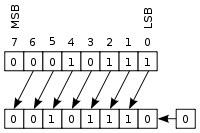
\includegraphics[scale=0.66]{14_bitfields/200px-Rotate_left_logically.png}
\caption{\IFRU{Как работает инструкция \SHL\protect\footnotemark}
{How \SHL instruction works\protect\footnotemark}}
\end{figure}

\footnotetext{\IFRU{иллюстрация взята из}{illustration taken from} wikipedia}

\index{x86!\Instructions!AND}
\IFRU{Макрос \TT{IS\_SET} на самом деле это операция логического И (\IT{AND}) 
и она возвращает $0$ если бита там нет, 
либо эту же битовую маску, если бит там есть. 
В \CCpp, конструкция \TT{if()} срабатывает, если выражение внутри её не ноль, пусть хоть $123456$, 
поэтому все будет работать.}
{The \TT{IS\_SET} macro is in fact logical and operation (\IT{AND}) 
and it returns $0$ if specific bit is absent there,
or bit mask, if the bit is present.
\IT{if()} operator triggered in \CCpp if expression in it is not a zero, it might be even $123456$, that is why
it always working correctly.}

\input{14_bitfields/shifts_x86}

\input{14_bitfields/shifts_ARM}



\subsection{\IFRU{Пример вычисления CRC32}{CRC32 calculation example}}
\index{CRC32}

\newcommand{\URLCRCSRC}{\url{http://burtleburtle.net/bob/c/crc.c}}

\IFRU{Это распространенный табличный способ вычисления хеша алгоритмом 
CRC32\footnote{Исходник взят тут: \URLCRCSRC}.}
{This is very popular table-based CRC32 hash calculation 
method\footnote{Source code was taken here: \URLCRCSRC}.}

\lstinputlisting{14_bitfields/CRC.c}

\index{\CLanguageElements!for}
\IFRU{Нас интересует функция \TT{crc()}. 
Кстати, обратите внимание на два инициализатора в выражении \TT{for()}: \TT{hash=len, i=0}. 
Стандарт \CCpp, конечно, допускает это. А в итоговом коде, вместо одной операции инициализации цикла, будет две.}
{We are interesting in the \TT{crc()} function only.
By the way, pay attention to two loop initializers in the \TT{for()} statement: \TT{hash=len, i=0}.
\CCpp standard allows this, of course.
Emitted code will contain two operations in loop initialization part
instead of usual one.}

\IFRU{Компилируем в MSVC с оптимизацией (\Ox). 
Для краткости, я приведу только функцию \TT{crc()}, с некоторыми комментариями.}
{Let's compile it in MSVC with optimization (\Ox).
For the sake of brevity, only \TT{crc()} function is listed here, with my comments.}

\lstinputlisting{\IFRU{14_bitfields/CRC_2_ru.asm}{14_bitfields/CRC_2_en.asm}}

\IFRU{Попробуем то же самое в GCC 4.4.1 с опцией \Othree:}
{Let's try the same in GCC 4.4.1 with \Othree option:}

\lstinputlisting{\IFRU{14_bitfields/CRC_gcc_O3_ru.asm}{14_bitfields/CRC_gcc_O3_en.asm}}

\index{x86!\Instructions!NOP}
\index{x86!\Instructions!LEA}
\IFRU{GCC немного выровнял начало тела цикла по 8-байтной границе, для этого добавил 
\NOP и \TT{lea esi, [esi+0]} (что тоже \IT{холостая операция}). 
Подробнее об этом смотрите в разделе о npad~\ref{sec:npad}.}
{GCC aligned loop start on a 8-byte border by adding \NOP and \TT{lea esi, [esi+0]} (that is \IT{idle operation} too).
Read more about it in npad section~\ref{sec:npad}.}




\section{\IFRU{Структуры}{Structures}}

\IFRU{В принципе, структура в \CCpp это, с некоторыми допущениями, просто всегда лежащий рядом, 
и в той же последовательности, набор переменных, не обязательно одного типа.}
{It can be defined that \CCpp structure, with some assumptions, just a set of variables, always stored
in memory together, not necessary of the same type.}

\subsection{\IFRU{Пример SYSTEMTIME}{SYSTEMTIME example}}

\newcommand{\FNSYSTEMTIME}{\footnote{\href{http://msdn.microsoft.com/en-us/library/ms724950(VS.85).aspx}{MSDN: SYSTEMTIME structure}}}

\IFRU{Возьмем, к примеру, структуру SYSTEMTIME\FNSYSTEMTIME{} из win32 описывающую время.}
{Let's take SYSTEMTIME\FNSYSTEMTIME{} win32 structure describing time.}

\IFRU{Она объявлена так:}{That's how it's defined:}

\begin{lstlisting}[caption=WinBase.h]
typedef struct _SYSTEMTIME {
  WORD wYear;
  WORD wMonth;
  WORD wDayOfWeek;
  WORD wDay;
  WORD wHour;
  WORD wMinute;
  WORD wSecond;
  WORD wMilliseconds;
} SYSTEMTIME, *PSYSTEMTIME;
\end{lstlisting}

\IFRU{Пишем на Си функцию для получения текущего системного времени:}
{Let's write a C function to get current time:}

\lstinputlisting{15_structs/systemtime.c}

\IFRU{Что в итоге}{We got} (MSVC 2010):

\lstinputlisting[caption=MSVC 2010]{15_structs/systemtime.asm}

\IFRU{Под структуру в стеке выделено 16 байт ~--- именно столько будет \TT{sizeof(WORD)*8}
(в структуре 8 переменных с типом WORD).}
{16 bytes are allocated for this structure in local stack ~--- that's exactly \TT{sizeof(WORD)*8}
(there are 8 WORD variables in the structure).}

\newcommand{\FNMSDNGST}{\footnote{\href{http://msdn.microsoft.com/en-us/library/ms724390(VS.85).aspx}{MSDN: GetSystemTime function}}}

\IFRU{Обратите внимание на тот факт что структура начинается с поля \TT{wYear}. 
Можно сказать что в качестве аргумента для \TT{GetSystemTime()}\FNMSDNGST передается указатель на структуру 
SYSTEMTIME, но можно также сказать, что передается указатель на поле \TT{wYear}, 
что одно и тоже! 
\TT{GetSystemTime()} пишет текущий год в тот WORD на который указывает переданный указатель, 
затем сдвигается на 2 байта вправо, пишет текущий месяц, итд, итд.}
{Pay attention to the fact the structure beginning with \TT{wYear} field.
It can be said, an pointer to SYSTEMTIME structure is passed to \TT{GetSystemTime()}\FNSYSTEMTIME,
but it's also can be said, pointer to \TT{wYear} field is passed, and that's the same!
\TT{GetSystemTime()} writting current year to the WORD pointer pointing to, then shifting 2 bytes
ahead, then writting current month, etc, etc.}

\IFRU{Тот факт что поля структуры это просто переменные расположенные рядом, 
я могу проиллюстрировать следующим образом.}
{The fact that structure fields are just variables located side-by-side, 
I can illustrate by the following method.}
\IFRU{Глядя на описание структуры}{Keeping in ming} \TT{SYSTEMTIME}\IFRU{, я могу переписать этот простой пример так:}
{ structure description, I can rewrite this simple example like this:}

\lstinputlisting{15_structs/systemtime2.c}

\IFRU{Компилятор немного поворчит:}{Compiler will warn us:}

\begin{lstlisting}
systemtime2.c(7) : warning C4133: 'function' : incompatible types - from 'WORD [8]' to 'LPSYSTEMTIME'
\end{lstlisting}

\IFRU{Тем не менее, выдаст такой код}{But nevertheless, it will produce this code}:

\lstinputlisting[caption=MSVC 2010]{15_structs/systemtime2.asm}

\IFRU{И это работает так же}{And it works just as the same}!

\IFRU{Любопытно что результат на ассемблере неотличим от предыдущего}{It's very interesting fact that
result in assembly form cannot be distinguished from the result of previous compilation}.
\IFRU{Таким образом, глядя на этот код, 
никогда нельзя сказать с уверенностью, была ли там объявлена структура, либо просто набор переменных.}
{So by looking at this code, one cannot say for sure, was there structure declared, or just pack of variables.} 

\IFRU{Тем не менее, никто в здравом уме делать так не будет}{Nevertheless, no one will do it in sane state of mind}.
\IFRU{Потому что это неудобно}{Because it's not handy}. 
\IFRU{К тому же, иногда, поля в структуре могут меняться разработчиками, 
переставляться местами, итд}{Also, structure fields may be changed by developers, swapped, etc}.



\subsection{\IFRU{Выделяем место для структуры через malloc()}{Let's allocate place for structure using malloc()}}

\IFRU{Однако, бывает и так, что проще хранить структуры не в стеке а в куче\footnote{heap}:}
{However, sometimes it's simpler to place structures not in local stack, but in heap:}

\lstinputlisting{15_structs/systemtime_malloc.c}

\IFRU{Скомпилируем на этот раз с оптимизацией (\Ox) чтобы было проще увидеть то, что нам нужно.}
{Let's compile it now with optimization (\Ox) so to easily see what we need.}

\lstinputlisting[caption=\Optimizing MSVC]{15_structs/systemtime_malloc.asm}

\index{\CStandardLibrary!malloc()}
\IFRU{Итак, \TT{sizeof(SYSTEMTIME) = 16}, именно столько байт выделяется при помощи \TT{malloc()}. 
Она возвращает указатель на только что выделенный блок памяти в \EAX, который копируется в \ESI. 
Win32 функция \TT{GetSystemTime()} обязуется сохранить состояние \ESI, 
поэтому здесь оно нигде не сохраняется и продолжает использоваться после вызова \TT{GetSystemTime()}.}
{So, \TT{sizeof(SYSTEMTIME) = 16}, that's exact number of bytes to be allocated by \TT{malloc()}.
It return the pointer to freshly allocated memory block in \EAX, which is then moved into \ESI.
\TT{GetSystemTime()} win32 function undertake to save \ESI value, 
and that's why it is not saved here and continue to be used after \TT{GetSystemTime()} call.}

\index{x86!\Instructions!MOVZX}
\IFRU{
Новая инструкция ~--- \MOVZX (\IT{Move with Zero eXtent}). 
Она нужна почти там же где и \MOVSX, 
только всегда очищает остальные биты в $0$. Дело в том что \printf требует 32-битный тип \Tint, 
а в структуре лежит WORD ~--- это 16-битный беззнаковый тип. Поэтому копируя значение из WORD в \Tint, 
нужно очистить биты от 16 до 31, иначе там будет просто случайный мусор, оставшийся от предыдущих действий 
с регистрами.}
{New instruction ~--- \MOVZX (\IT{Move with Zero eXtent}).
It may be used almost in those cases as \MOVSX, but, it clearing other bits to $0$.
That's because \printf require 32-bit \Tint, but we got WORD in structure ~--- that's 16-bit unsigned type.
That's why by copying value from WORD into \Tint{}, bits from 16 to 31 should be cleared, 
because there will be random noise otherwise, leaved from previous operations on registers.}

\IFRU{В этом примере я тоже могу представить структуру как массив WORD-ов}{In this example, I can represent
structure as array of WORD-s}:

\lstinputlisting{15_structs/systemtime_malloc2.c}

\IFRU{Получим такое}{We got}:

\lstinputlisting[caption=\Optimizing MSVC]{15_structs/systemtime_malloc2.asm}

\IFRU{И снова мы получаем идетичный код, неотличимый от предыдущего}{Again, we got a code that cannot be distinguished
from previous}.
\IFRU{Но и снова я должен отметить, что в реальности так лучше не делать}{And again I should note, one shouldn't do
this in practice}.



\subsection{struct tm}

\subsubsection{Linux}

\IFRU{В Линуксе, для примера, возьем структуру \TT{tm} из \TT{time.h}:}
{As of Linux, let's take \TT{tm} structure from \TT{time.h} for example:}

\lstinputlisting{15_structs/GCC_tm.c}

\IFRU{Компилируем при помощи}{Let's compile it in} GCC 4.4.1:

\IFRU{\lstinputlisting[caption=GCC 4.4.1]{15_structs/GCC_tm_ru.asm}}{\lstinputlisting{15_structs/GCC_tm_en.asm}}

\IFRU{К сожалению, по какой-то причине, \IDA не сформировала названия локальных переменных в стеке. 
Но так как мы уже опытные реверсеры :-) то можем обойтись и без этого в таком простом примере.}
{Somehow, \IDA didn't created local variables names in local stack.
But since we already experienced reverse engineers :-) we may do it without this information in 
this simple example.}

\IFRU{Обратите внимание на \TT{lea edx, [eax+76Ch]} ~--- эта инструкция прибавляет $0x76C$ к \EAX, 
но не модифицирует флаги. См. также соответствующий раздел об инструкции \LEA{}~\ref{sec:LEA}.}
{Please also pay attention to \TT{lea edx, [eax+76Ch]} ~--- this instruction just adding $0x76C$ to \EAX,
but not modify any flags. See also relevant section about \LEA{}~\ref{sec:LEA}.}

Чтобы проиллюстрировать то что структура это просто набор переменных лежащих в одном месте, переделаем немного
пример, заглянув предварительно в файл time.h:

\begin{lstlisting}[caption=time.h]
struct tm
{
  int	tm_sec;
  int	tm_min;
  int	tm_hour;
  int	tm_mday;
  int	tm_mon;
  int	tm_year;
  int	tm_wday;
  int	tm_yday;
  int	tm_isdst;
};
\end{lstlisting}

\lstinputlisting{15_structs/GCC_tm2.c}

Обратите внимание на то что в \TT{localtime\_r} передается указатель именно на \TT{tm\_sec}, 
т.е., на первый элемент ``структуры''.

В итоге, и этот компилятор поворчит:

\begin{lstlisting}[caption=GCC 4.7.3]
GCC_tm2.c: In function 'main':
GCC_tm2.c:11:5: warning: passing argument 2 of 'localtime_r' from incompatible pointer type [enabled by default]
In file included from GCC_tm2.c:2:0:
/usr/include/time.h:59:12: note: expected 'struct tm *' but argument is of type 'int *'
\end{lstlisting}

Тем не менее, сгенерирует такоу:

\lstinputlisting[caption=GCC 4.7.3]{15_structs/GCC_tm2.asm}

Этот код почти идентичен уже рассмотренному, и нельзя сказать, была ли структура
в оригинальном исходном коде либо набор переменных.

И это работает. Однако, в реальности так лучше не делать. Обычно, компилятор располагает переменные в локальном
стеке в том же порядке, в котором они объявляются в функции. Тем не менее, никакой гарантии нет.

Кстати, какой-нибудь другой компилятор может предупредить, что переменные \TT{tm\_year}, \TT{tm\_mon}, \TT{tm\_mday},
\TT{tm\_hour}, \TT{tm\_min}, но не \TT{tm\_sec}, используются без инициализации. 
Действительно, ведь компилятор не знает
что они будут заполнены при вызове функции \TT{localtime\_r()}.

Я выбрал именно этот пример для иллюстрации, потому что члены структуры имеют тип \Tint, а члены структуры
\TT{SYSTEMTIME} ~--- 16-битные \TT{WORD}, и если их объявлять так же, то они будут выровнены по 32-битной границе 
и ничего не выйдет (потому что \TT{GetSystemTime()} заполнит их неверно). Читайте об этом в следующей секции
``\StructurePackingSectionName''.

\index{\SyntacticSugar}
Так что, структура это просто набор переменных лежащих в одном месте, рядом. Я мог бы сказать что структура
это такой синтаксический сахар, заставляющий компилятор удерживать их в одном месте. Впрочем, я не специалист
по языкам программирования, так что, скорее всего, ошибаюсь с этим термином.
Кстати, когда-то, в очень ранних версиях Си (перед 1972) структур не 
было вовсе\cite{Ritchie:1993:DCL:155360.155580}.

\subsubsection{ARM + \OptimizingKeil + \ThumbMode}

Этот же пример:

\lstinputlisting[caption=\OptimizingKeil + \ThumbMode]{15_structs/tm_ARM_keil_thumb.asm}

\subsubsection{ARM + \OptimizingXcode + \ThumbTwoMode}

\IDA ``узнала'' структуру tm (потому что \IDA ``знает'' типы аргументов библиотечных функций, 
таких как \TT{localtime\_r()}), поэтому показала здесь обращения к элементам структуры.

\lstinputlisting[caption=\OptimizingXcode + \ThumbTwoMode]{15_structs/tm_ARM_xcode_thumb.asm}



\subsection{\StructurePackingSectionName}

\IFRU{Достаточно немаловажный момент, это упаковка полей в структурах\footnote{См.также: \URLWPDA}.}
{One important thing is fields packing in structures\footnote{See also: \URLWPDA}.}

\IFRU{Возьмем простой пример:}{Let's take a simple example:}

\lstinputlisting{15_structs/packing.c}

\IFRU{Как видно, мы имеем два поля \Tchar (занимающий один байт) и еще два ~--- \Tint (по 4 байта).}
{As we see, we have two \Tchar fields (each is exactly one byte) and two more ~--- \Tint (each - 4 bytes).}

\subsubsection{x86}

\IFRU{Компилируется это все в:}{That's all compiling into:}

\lstinputlisting{15_structs/packing.asm}

\IFRU{Мы видим здесь что адрес каждого поля в структуре выравнивается по 4-байтной границе. 
Так что каждый \Tchar здесь занимает те же 4 байта что и \Tint. Зачем? 
Затем что процессору удобнее обращаться по таким адресам и кешировать данные из памяти.}
{As we can see, each field's address is aligned on a 4-bytes border.
That's why each \Tchar occupies 4 bytes here (like \Tint). Why?
Thus it is easier for CPU to access memory at aligned addresses and to cache data from it.}

\IFRU{Но это не экономично по размеру данных.}{However, it is not very economical in size sense.}

\IFRU{Попробуем скомпилировать тот же исходник с опцией}{Let's try to compile it with option} (\TT{/Zp1}) 
(\IT{/Zp[n] pack structs on n-byte boundary}).

\lstinputlisting[caption=MSVC /Zp1]{15_structs/packing_msvc_Zp1.asm}

\IFRU{Теперь структура занимает 10 байт и все \Tchar занимают по байту. Что это дает? 
Экономию места. Недостаток ~--- процессор будет обращаться к этим полям не так эффективно 
по скорости как мог бы.}
{Now the structure takes only 10 bytes and each \Tchar value takes 1 byte. What it give to us?
Size economy. And as drawback ~--- CPU will access these fields without maximal performance it can.}

\IFRU{Как нетрудно догадаться, если структура используется много в каких исходниках и объектных файлах, 
все они должны быть откомпилированы с одним и тем же соглашением об упаковке структур.}
{As it can be easily guessed, if the structure is used in many source and object files,
all these should be compiled with the same convention about structures packing.}

\newcommand{\FNURLMSDNZP}{\footnote{\href{http://msdn.microsoft.com/en-us/library/ms253935.aspx}
{MSDN: Working with Packing Structures}}}
\newcommand{\FNURLGCCPC}{\footnote{\href{http://gcc.gnu.org/onlinedocs/gcc/Structure_002dPacking-Pragmas.html}
{Structure-Packing Pragmas}}}

\IFRU{Помимо ключа MSVC \TT{/Zp}, указывающего, по какой границе упаковывать поля структур, есть также 
опция компилятора \TT{\#pragma pack}, её можно указывать прямо в исходнике. 
Это справедливо и для MSVC\FNURLMSDNZP и GCC\FNURLGCCPC{}.}
{Aside from MSVC \TT{/Zp} option which set how to align each structure field, here is also
\TT{\#pragma pack} compiler option, it can be defined right in source code.
It is available in both MSVC\FNURLMSDNZP and GCC\FNURLGCCPC{}.}

\IFRU{Давайте теперь вернемся к \TT{SYSTEMTIME}, которая состоит из 16-битных полей. 
Откуда наш компилятор знает что их надо паковать по однобайтной границе?}
{Let's back to the \TT{SYSTEMTIME} structure consisting in 16-bit fields.
How our compiler know to pack them on 1-byte alignment method?}

\IFRU{В файле \TT{WinNT.h} попадается такое:}{\TT{WinNT.h} file has this:}

\begin{lstlisting}[caption=WinNT.h]
#include "pshpack1.h"
\end{lstlisting}

\IFRU{И такое:}{And this:}

\begin{lstlisting}[caption=WinNT.h]
#include "pshpack4.h"                   // 4 byte packing is the default
\end{lstlisting}

\IFRU{Сам файл PshPack1.h выглядит так:}{The file PshPack1.h looks like:}

\begin{lstlisting}[caption=PshPack1.h]
#if ! (defined(lint) || defined(RC_INVOKED))
#if ( _MSC_VER >= 800 && !defined(_M_I86)) || defined(_PUSHPOP_SUPPORTED)
#pragma warning(disable:4103)
#if !(defined( MIDL_PASS )) || defined( __midl )
#pragma pack(push,1)
#else
#pragma pack(1)
#endif
#else
#pragma pack(1)
#endif
#endif /* ! (defined(lint) || defined(RC_INVOKED)) */
\end{lstlisting}

\IFRU{Собственно, так и задается компилятору, как паковать объявленные после \TT{\#pragma pack} структуры.}
{That's how compiler will pack structures defined after \TT{\#pragma pack}.}

\subsubsection{ARM + \OptimizingKeil + \ThumbMode}

\lstinputlisting[caption=\OptimizingKeil + \ThumbMode]{15_structs/packing_Keil_thumb.asm}

\IFRU{Как мы помним, здесь передается не указатель на структуру, а сама структура, а так как в ARM первые 4 аргумента
функции передаются через регистры, то поля структуры передаются через}
{As we may recall, here a structure passed instead of pointer to structure,
and since first 4 function arguments in ARM are passed via registers,
so then structure fields are passed via} \TT{R0-R3}.

\index{ARM!\Instructions!LDRB}
\index{x86!\Instructions!MOVSX}
\IFRU{Инструкция }\TT{LDRB} \IFRU{загружает один байт из памяти и расширяет до 32-бит учитывая знак.}
{loads one byte from memory and extending it to 32-bit, taking into account its sign.}
\IFRU{Это похоже на инструкцию}{This is similar to} \MOVSX \IFRU{в}{instruction in} x86.
\IFRU{Она здесь применяется дла загрузки полей}{Here it is used for loading fields} $a$ \AndENRU $c$ 
\IFRU{из структуры}{from structure}.

\index{Function epilogue}
\IFRU{Еще что бросается в глаза, так это то что вместо эпилога функции, переход на эпилог другой функции!}
{One more thing we spot easily, instead of function epilogue, here is jump to another function's epilogue!}
\IFRU{Действительно, то была совсем другая, не относящаяся к этой, функция, однако, она имела точно такой же
эпилог}{Indeed, that was another function, not related in any way to our function, however, it has exactly
the same epilogue} 
(\IFRU{видимо, тоже хранила в стеке 5 локальных переменных}{probably because, it hold 5 local variables too} 
($5*4=0x14$)).
\IFRU{К тому же, она находится рядом (обратите внимание на адреса).}
{Also it is located nearly (take a look on addresses).}
\IFRU{Действительно, нет никакой разницы, какой эпилог исполнять, если он работает так же как нам нужно.}
{Indeed, there are no difference, which epilogue to execute, if it works just as we need.}
\IFRU{Keil решил сделать так, вероятно, из-за экономии.}{Apparently, Keil decides to do this by a reason of economy.}
\IFRU{Эпилог занимает 4 байта, а переход ~--- только 2.}{Epilogue takes 4 bytes while jump ~--- only 2.}

\subsubsection{ARM + \OptimizingXcode + \ThumbTwoMode}

\lstinputlisting[caption=\OptimizingXcode + \ThumbTwoMode]{15_structs/packing_Xcode_thumb.asm}

\index{ARM!\Instructions!SXTB}
\index{x86!\Instructions!MOVSX}
\TT{SXTB} (\IT{Signed Extend Byte}) \IFRU{это так же аналог}{is analogous to} \MOVSX \In 
x86\IFRU{, только работает не с памятью, а с регистром.}{ as well, but works not with memory, but with register.}
\IFRU{Всё остальное ~--- так же.}{All the rest ~--- just the same.}



\subsection{\IFRU{Вложенные структуры}{Nested structures}}

\IFRU{Теперь, как насчет ситуаций, когда одна структура определяет внутри себя еще одну структуру?}
{Now what about situations when one structure defines another structure inside?}

\lstinputlisting{15_structs/nested.c}

\dots \IFRU{в этом случае, оба поля \TT{inner\_struct} просто будут располагаться между полями a,b и d,e в 
\TT{outer\_struct}.}
{in this case, both \TT{inner\_struct} fields will be placed between a,b and d,e fields of
\TT{outer\_struct}.}

\IFRU{Компилируем}{Let's compile} (MSVC 2010):

\lstinputlisting[caption=MSVC 2010]{15_structs/nested_msvc.asm}

\IFRU{Очень любопытный момент в том, что глядя на этот код на ассемблере, мы даже не видим, 
что была использована какая-то еще другая структура внутри этой!
Так что, пожалуй, можно сказать, что все вложенные структуры в итоге разворачиваются в одну, \IT{линейную} 
или \IT{одномерную} структуру.}
{One curious point here is that by looking onto this assembly code, we do not even see that
another structure was used inside of it!
Thus, we would say, nested structures are finally unfolds into \IT{linear} or \IT{one-dimensional} structure.}

\IFRU{Конечно, если заменить объявление \TT{struct inner\_struct c;} на \TT{struct inner\_struct *c;} 
(объявляя таким образом указатель), ситауция будет совсем иная.}
{Of course, if to replace \TT{struct inner\_struct c;} declaration to \TT{struct inner\_struct *c;} 
(thus making a pointer here) situation will be significally different.}



\subsection{\IFRU{Работа с битовыми полями в структуре}{Bit fields in structure}}

\subsubsection{\IFRU{Пример CPUID}{CPUID example}}

\IFRU{Язык \CCpp позволяет укзывать, сколько именно бит отвести для каждого поля структуры. 
Это удобно если нужно экономить место в памяти. К примеру, для переменной типа \Tbool достаточно одного бита.
Но, это не очень удобно, если нужна скорость.}
{\CCpp language allow to define exact number of bits for each structure fields.
It is very useful if one needs to save memory space. 
For example, one bit is enough for variable of \Tbool type.
But of course, it is not rational if speed is important.}

\newcommand{\FNCPUID}{\footnote{\url{http://en.wikipedia.org/wiki/CPUID}}}

\index{x86!\Instructions!CPUID}
\IFRU{Рассмотрим пример с инструкцией \CPUID\FNCPUID. 
Эта инструкция возвращает информацию о том, какой процессор имеется в наличии и какие фичи он имеет.}
{Let's consider \CPUID\FNCPUID instruction example.
This instruction returning information about current CPU and its features.}

\IFRU{Если перед исполнением инструкции в \EAX будет 1, 
то \CPUID вернет упакованную в \EAX такую информацию о процессоре:}
{If the \EAX is set to 1 before instruction execution, 
\CPUID will return this information packed into the \EAX register:}

\begin{center}
\begin{tabular}{ | l | l | }
\hline
3:0 & Stepping \\
7:4 & Model \\
11:8 & Family \\
13:12 & Processor Type \\
19:16 & Extended Model \\
27:20 & Extended Family \\
\hline
\end{tabular}
\end{center}

\newcommand{\FNGCCAS}{\footnote{\href{http://www.ibiblio.org/gferg/ldp/GCC-Inline-Assembly-HOWTO.html}
{\IFRU{Подробнее о встроенном ассемблере GCC}{More about internal GCC assembler}}}}

\IFRU{MSVC 2010 имеет макрос для \CPUID, а GCC 4.4.1 ~--- нет. 
Поэтому для GCC сделаем эту функцию сами, используя его встроенный ассемблер\FNGCCAS.}
{MSVC 2010 has \CPUID macro, but GCC 4.4.1 ~--- has not.
So let's make this function by yourself for GCC with the help of its built-in assembler\FNGCCAS.}

\lstinputlisting{15_structs/CPUID.c}

\IFRU{После того как \CPUID заполнит \EAX/\EBX/\ECX/\EDX, у нас они отразятся в массиве \TT{b[]}. 
Затем, мы имеем указатель на структуру \TT{CPUID\_1\_EAX}, и мы указываем его на значение 
\EAX из массива \TT{b[]}.}
{After \CPUID will fill \EAX/\EBX/\ECX/\EDX, these registers will be reflected in the \TT{b[]} array.
Then, we have a pointer to the \TT{CPUID\_1\_EAX} structure and we point it to the value in the \EAX from \TT{b[]} array.}

\IFRU{Иными словами, мы трактуем 32-битный \Tint как структуру.}
{In other words, we treat 32-bit \Tint value as a structure.}

\IFRU{Затем мы читаем из структуры.}{Then we read from the stucture.}

\IFRU{Компилируем в MSVC 2008 с опцией \Ox}{Let's compile it in MSVC 2008 with \Ox option}:

\lstinputlisting[caption=\Optimizing MSVC 2008]{15_structs/CPUID_msvc_Ox.asm}

\index{x86!\Instructions!SHR}
\IFRU{Инструкция \TT{SHR} сдвигает значение из \EAX на то количество бит, 
которое нужно \IT{пропустить}, то есть, мы игнорируем некоторые биты \IT{справа}.}
{\TT{SHR} instruction shifting value in the \EAX register by number of bits should be
\IT{skipped}, e.g., we ignore a bits \IT{at right}.}

\index{x86!\Instructions!AND}
\IFRU{А инструкция \ANDIns очищает биты \IT{слева} которые нам не нужны, или же, говоря иначе, 
она оставляет по маске только те биты в \EAX, которые нам сейчас нужны.}
{\ANDIns instruction clears bits not needed \IT{at left}, or, in other words, 
leaves only those bits in the \EAX register we need now.}

\IFRU{Попробуем GCC 4.4.1 с опцией \Othree.}{Let's try GCC 4.4.1 with \Othree option.}

\lstinputlisting[caption=\Optimizing GCC 4.4.1]{15_structs/CPUID_gcc_O3.asm}

\IFRU{Практически, то же самое. Единственное что стоит отметить это то, что GCC решил зачем-то объеденить 
вычисление \TT{extended\_model\_id} и \TT{extended\_family\_id} в один блок, 
вместо того чтобы вычислять их перед соответствующим вызовом \printf.}
{Almost the same. The only thing worth noting is that GCC somehow united calculation of
\TT{extended\_model\_id} and \TT{extended\_family\_id} into one block,
instead of calculating them separately, before corresponding each \printf call.}

\subsubsection{\WorkingWithFloatAsWithStructSubSubSectionName}
\label{sec:floatasstruct}

\IFRU{Как уже раннее указывалось в секции о FPU~\ref{sec:FPU}, и \Tfloat и \Tdouble содержат в себе знак, 
мантиссу и экспоненту. 
Однако, можем ли мы работать с этими полями напрямую? Попробуем с \Tfloat.}
{As it was already noted in section about FPU~\ref{sec:FPU}, both \Tfloat and \Tdouble types consisted of sign,
significand (or fraction) and exponent.
But will we able to work with these fields directly? Let's try with \Tfloat.}

\index{IEEE 754}
\index{float}
\begin{figure}[ht!]
\centering
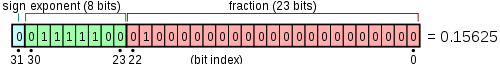
\includegraphics[scale=0.66]{15_structs/500px-Float_example.png}
\caption{\IFRU{Формат значения float\protect\footnotemark}
{float value format\protect\footnotemark}}
\end{figure}

\footnotetext{\IFRU{иллюстрация взята из}{illustration taken from} wikipedia}

\lstinputlisting{15_structs/float_en.c}

\IFRU{Структура \TT{float\_as\_struct} занимает в памяти столько же места сколько и \Tfloat, 
то есть 4 байта или 32 бита.}
{\TT{float\_as\_struct} structure occupies as much space is memory as \Tfloat, e.g., 4 bytes or 32 bits.}

\IFRU{Далее мы выставляем во входящем значении отрицательный знак, 
а также прибавляя двойку к экспоненте, мы тем 
самым умножаем всё значение на \TT{$2^2$}, то есть на 4.}
{Now we setting negative sign in input value and also by addding 2 to exponent we thereby multiplicating
the whole number by \TT{$2^2$}, e.g., by 4.}

\IFRU{Компилируем в MSVC 2008 без оптимизации:}{Let's compile in MSVC 2008 without optimization:}

\lstinputlisting[caption=\NonOptimizing MSVC 2008]
{\IFRU{15_structs/float_msvc_ru.asm}{15_structs/float_msvc_en.asm}}

\IFRU{Слекга избыточно. В версии скомпилированной с флагом \Ox нет вызовов \TT{memcpy()}, 
там работа происходит сразу с переменной f. Но по неоптимизированной версии будет проще понять.}
{Redundant for a bit.
If it is compiled with \Ox flag there is no \TT{memcpy()} call,
\TT{f} variable is used directly.
But it is easier to understand it all considering unoptimized version.}

\IFRU{А что сделает GCC 4.4.1 с опцией \TT{-O3}?}{What GCC 4.4.1 with \TT{-O3} will do?}

\lstinputlisting[caption=\Optimizing GCC 4.4.1]
{\IFRU{15_structs/float_gcc_O3_ru.asm}{15_structs/float_gcc_O3_en.asm}}

\IFRU{Да, функция \TT{f()} в целом понятна. Однако, что интересно, еще при компиляции, 
не взирая на мешанину с полями структуры, GCC умудрился вычислить результат функции \TT{f(1.234)} и 
сразу подставить его в аргумент для \printf{}!}
{The \TT{f()} function is almost understandable. However, what is interesting, GCC was able to calculate
\TT{f(1.234)} result during compilation stage despite all this hodge-podge with structure fields
and prepared this argument to the \printf{} as precalculated!}





\section{\IFRU{Классы в Си++}{C++ classes}}

\subsection{\IFRU{Простой пример}{Simple example}}

\IFRU{Я намеренно расположил описание классов здесь сразу за структурами, 
потому что внутреннее представление классов в Си++ почти такое же как и представление структур.}
{I placed the section about C++ classes here intentionally after structures description,
because internally, C++ classes representation is almost the same as structures representation.}

\IFRU{Давайте попробуем простой пример с двумя переменными, двумя конструкторами и одним методом:}
{Let's try an example with two variables, two constructors and one method:}

\lstinputlisting{16_classes/16_1.cpp}

\IFRU{Вот как выглядит \main на ассемблере:}{Here is how \main function looks like translated 
into assembly language:}

\lstinputlisting{16_classes/16_1_msvc.asm}

\IFRU{Вот что происходит. 
Под каждый экземпляр класса \IT{c} выделяется по 8 байт, столько же, сколько нужно 
для хранения двух переменных.}
{So what's going on.
For each object (instance of class \IT{c}) 8 bytes allocated, that's exactly size of 2 variables storage.}

\IFRU{Для \IT{c1} вызывается конструктор по умолчанию без аргументов \TT{??0c@@QAE@XZ}. 
Для \IT{c2} вызывается другой конструктор \TT{??0c@@QAE@HH@Z} и передаются два числа в качестве аргументов.}
{For \IT{c1} a default argumentless constructor \TT{??0c@@QAE@XZ} is called.
For \IT{c2} another constructor \TT{??0c@@QAE@HH@Z} is called and two numbers are passed as arguments.}

\index{this}
\index{x86!\Registers!ECX}
\IFRU{А указатель на объект (\IT{this} в терминологии Си++) передается в регистре \ECX. 
Это называется thiscall~\ref{thiscall} ~--- метод передачи указателя на объект.}
{A pointer to object (\IT{this} in C++ terminology) is passed in the \ECX register.
This is called thiscall~\ref{thiscall} ~--- a pointer to object passing method.}

\IFRU{В данном случае, MSVC делает это через \ECX. Необходимо помнить, что это не стандартизированный метод, 
и другие компиляторы могут делать это иначе, например через первый аргумент функции (как GCC).}
{MSVC doing it using the \ECX register. Needless to say, it is not a standardized method, other compilers could do it
differently, e.g., via first function argument (like GCC).}

%\newcommand{\URLNM}{\href{http://en.wikipedia.org/wiki/Visual_C\%2B\%2B_name_mangling}{Wikipedia: Visual C++ name mangling}}
\newcommand{\URLNM}{\href{http://en.wikipedia.org/wiki/Name_mangling}{Wikipedia: Name mangling}}

\label{namemangling}
\index{Name mangling}
\IFRU{Почему у имен функций такие странные имена? Это \IT{name mangling}\footnote{\URLNM}.}
{Why these functions has so odd names? That's \IT{name mangling}\footnote{\URLNM}.}

\IFRU{В Си++, у класса, может иметься несколько методов с одинаковыми именами 
но аргументами разных типов ~--- это полиморфизм. 
Ну и конечно, у разных классов могут быть методы с одинаковыми именами.}
{C++ class may contain several methods sharing the same name but having different arguments ~--- 
that's polymorphism.
And of course, different classes may own methods sharing the same name.}

\index{\IFRU{Компоновщик}{Linker}}
\IFRU{\IT{Name mangling} позволяет закодировать имя класса + имя метода + типы всех аргументов метода 
в одной ASCII-строке, которая затем используется как внутреннее имя функции. 
Это все потому что ни компоновщик\footnote{linker}, ни загрузчик DLL \ac{OS}
(мангленные имена могут быть среди экспортов/импортов в DLL), 
ничего не знают о Си++ или ООП.}
{\IT{Name mangling} enable us to encode class name + method name + all method argument types
in one ASCII-string, which is to be used as internal function name.
That's all because neither linker, nor DLL \ac{OS} loader (mangled names may be among 
DLL exports as well) knows nothing about C++ or OOP.}

\IFRU{Далее вызывается два раза \TT{dump()}.}{\TT{dump()} function called two times after.}

\IFRU{Теперь смотрим на код в конструкторах:}{Now let's see constructors' code:}

\lstinputlisting{16_classes/16_2_msvc.asm}

\IFRU{Конструкторы это просто функции, они используют указатель на структуру в \ECX, 
перекладывают его себе в локальную переменную, хотя это и не обязательно.}
{Constructors are just functions, they use pointer to structure in the \ECX,
moving the pointer into own local variable, however, it is not necessary.}

\IFRU{И еще метод \TT{dump()}:}{Now \TT{dump()} method:}

\lstinputlisting{16_classes/16_3_msvc.asm}

\IFRU{Все очень просто, \TT{dump()} берет указатель на структуру состоящую из двух \Tint через \ECX, 
выдергивает оттуда две переменные и передает их в \printf.}
{Simple enough: \TT{dump()} taking pointer to the structure containing two \Tint's in the \ECX,
takes two values from it and passing it into \printf.}

\IFRU{А если скомпилировать с оптимизацией (\Ox), то будет намного меньше всего:}
{The code is much shorter if compiled with optimization (\Ox):}

\lstinputlisting{16_classes/16_4_msvc_Ox.asm}

\index{x86!\Instructions!RET}
\IFRU{Вот и все. Единственное о чем еще нужно сказать, это о том что в функции \main, 
когда вызывался второй конструктор с двумя аргументами, за ним не корректировался стек при помощи 
\TT{add esp, X}. В то же время, в конце конструктора вместо \RET имеется \TT{RET 8}.}
{That's all. One more thing to say is that stack pointer was not corrected
with \TT{add esp, X} after constructor called. 
Withal, constructor has \TT{ret 8} instead of the \RET at the end.}

\index{thiscall}
\IFRU{Это потому что здесь используется thiscall~\ref{thiscall}, который, вместе с stdcall~\ref{stdcall} 
(все это ~--- методы передачи аргументов через стек), предлагает вызываемой функции корректировать стек. 
Инструкция \TT{ret X} сначала прибавляет \TT{X} к \ESP, затем передает управление вызывающей функции.}
{This is all because here used thiscall~\ref{thiscall} calling convention, the method of passing values through the
stack, which is, together with stdcall~\ref{stdcall} method, offers to correct stack to callee 
rather then to caller.
\TT{ret x} instruction adding \TT{X} to the value in the \ESP, then passes control to the caller function.}

\IFRU{См.также в соответствующем разделе о способах передачи аргументов через стек}
{See also section about calling conventions}~\ref{sec:callingconventions}.

\IFRU{Еще, кстати, нужно отметить, что именно компилятор решает, когда вызывать конструктор и деструктор ~--- 
но это итак известно из основ языка Си++.}
{It is also should be noted that compiler deciding when to call constructor and destructor ~--- but that's 
we already know from C++ language basics.}

\subsubsection{GCC}

\IFRU{В GCC 4.4.1 все почти так же, за исключением некоторых различий.}
{It is almost the same situation in GCC 4.4.1, with few exceptions.}

\lstinputlisting{16_classes/16_5_gcc.asm}

\newcommand{\URLAGNER}{\url{http://www.agner.org/optimize/calling_conventions.pdf}}

\IFRU{Здесь мы видим что применяется иной \IT{name mangling} характерный для стандартов 
GNU\footnote{Еще о name mangling разных компиляторов: \URLAGNER}. Во-вторых, указатель на экземпляр передается как первый аргумент функции ~--- конечно же, скрыто от программиста.}
{Here we see another \IT{name mangling} style, specific to GNU\footnote{One more document about different compilers name mangling types: \URLAGNER} standards. It is also can be noted that pointer to object is passed as first function argument ~--- hiddenly from programmer, of course.}

\IFRU{Это первый конструктор:}{First constructor:}

\begin{lstlisting}
                public _ZN1cC1Ev ; weak
_ZN1cC1Ev       proc near               ; CODE XREF: main+10

arg_0           = dword ptr  8

                push    ebp
                mov     ebp, esp
                mov     eax, [ebp+arg_0]
                mov     dword ptr [eax], 667
                mov     eax, [ebp+arg_0]
                mov     dword ptr [eax+4], 999
                pop     ebp
                retn
_ZN1cC1Ev       endp
\end{lstlisting}

\IFRU{Он просто записывает два числа по указателю переданному в первом (и единственном) аргументе.}
{What it does is just writes two numbers using pointer passed in first (and single) argument.}

\IFRU{Второй конструктор:}{Second constructor:}

\begin{lstlisting}
                public _ZN1cC1Eii
_ZN1cC1Eii      proc near

arg_0           = dword ptr  8
arg_4           = dword ptr  0Ch
arg_8           = dword ptr  10h

                push    ebp
                mov     ebp, esp
                mov     eax, [ebp+arg_0]
                mov     edx, [ebp+arg_4]
                mov     [eax], edx
                mov     eax, [ebp+arg_0]
                mov     edx, [ebp+arg_8]
                mov     [eax+4], edx
                pop     ebp
                retn
_ZN1cC1Eii      endp
\end{lstlisting}

\IFRU{Это функция, аналог которой мог бы выглядеть так:}{This is a function, analog of which could be looks like:}

\begin{lstlisting}
void ZN1cC1Eii (int *obj, int a, int b)
{
  *obj=a;
  *(obj+1)=b;
};
\end{lstlisting}

\IFRU{\dots что, в общем, предсказуемо.}{\dots and that's completely predictable.}

\IFRU{И функция \TT{dump()}:}{Now \TT{dump()} function:}

\begin{lstlisting}
                public _ZN1c4dumpEv
_ZN1c4dumpEv    proc near

var_18          = dword ptr -18h
var_14          = dword ptr -14h
var_10          = dword ptr -10h
arg_0           = dword ptr  8

                push    ebp
                mov     ebp, esp
                sub     esp, 18h
                mov     eax, [ebp+arg_0]
                mov     edx, [eax+4]
                mov     eax, [ebp+arg_0]
                mov     eax, [eax]
                mov     [esp+18h+var_10], edx
                mov     [esp+18h+var_14], eax
                mov     [esp+18h+var_18], offset aDD ; "%d; %d\n"
                call    _printf
                leave
                retn
_ZN1c4dumpEv    endp
\end{lstlisting}

\IFRU{Эта функция \IT{во внутреннем представлении} имеет один аргумент, через который передается указатель на 
объект\footnote{экземпляр класса} (\IT{this}).}
{This function in its \IT{internal representation} has sole argument, 
used as pointer to the object (\IT{this}).}

\IFRU{Таким образом, если брать в учет только эти простые примеры, разница между MSVC и GCC 
в способе кодирования имен функций (\IT{name mangling}) и передаче указателя на экземпляр класса 
(через \ECX или через первый аргумент).}
{Thus, if to base our judgment on these simple examples, the difference between MSVC and GCC
is style of function names encoding (\IT{name mangling}) and passing pointer to object
(via the \ECX register or via the first argument).}

\subsection{\IFRU{Наследование классов в C++}{Class inheritance in C++}}

\IFRU{О наследованных классах можно сказать что это та же простая структура которую мы уже рассмотрели, 
только расширяемая в наследуемых классах.}
{It can be said about inherited classes that it is simple structure we already considered, but extending 
in inherited classes.}

\IFRU{Возьмем очень простой пример}{Let's take simple example}:

\lstinputlisting{16_classes/classes1_inheritance.cpp}

\IFRU{Исследуя сгенерированный код для функций/методов \TT{dump()}, а также \TT{object::print\_color()},
посмотрим какая будет разметка памяти для структур-объектов (для 32-битного кода).}
{Let's investigate generated code of the \TT{dump()} functions/methods and also \TT{object::print\_color()},
let's see memory layout for structures-objects (as of 32-bit code).}

\index{Inline code}
\IFRU{Итак, методы \TT{dump()} разных классов сгенерированные MSVC 2008 с опциями \Ox и \Obzero}
{So, \TT{dump()} methods for several classes, generated by MSVC 2008 with \Ox and \Obzero options}
\footnote{\IFRU{опция \Obzero означает отмену inline expansion, 
ведь вставка компилятором тела функции/метода прямо в код где он вызывается только затруднит наши эксперименты}{
\Obzero options means inline expansion disabling since function inlining right into the code where the function
is called will make our experiment harder}}

\lstinputlisting[caption=\Optimizing MSVC 2008 /Ob0]{16_classes/classes1_1.asm}

\lstinputlisting[caption=\Optimizing MSVC 2008 /Ob0]{16_classes/classes1_2.asm}

\lstinputlisting[caption=\Optimizing MSVC 2008 /Ob0]{16_classes/classes1_3.asm}

\IFRU{Итак, разметка полей получается следующая}{So, here is memory layout}:

\IFRU{(базовый класс \IT{object})}{(base class \IT{object})}

\begin{center}
\begin{tabular}{ | l | l | }
\hline
  \tableheader{} \\
  +0x0 & int color \\
\hline
\end{tabular}
\end{center}

\IFRU{(унаследованные классы)}{(inherited classes)}

\IT{box}:

\begin{center}
\begin{tabular}{ | l | l | }
\hline
  \tableheader{} \\
  +0x0 & int color \\
  +0x4 & int width \\
  +0x8 & int height \\
  +0xC & int depth \\
\hline
\end{tabular}
\end{center}

\IT{sphere}:

\begin{center}
\begin{tabular}{ | l | l | }
\hline
  \tableheader{} \\
  +0x0 & int color \\
  +0x4 & int radius \\
\hline
\end{tabular}
\end{center}

\IFRU{Посмотрим тело \main}{Let's see \main function body}:

\lstinputlisting[caption=\Optimizing MSVC 2008 /Ob0]{16_classes/classes1_4.asm}

\IFRU{Наследованные классы всегда должны добавлять свои поля после полей базового класса для того, чтобы методы
базового класса могли продолжать работать со своими полями.}
{Inherited classes must always add their fields after base classes' fields, so to make possible for base 
class methods to work with their fields.}

\IFRU{Когда метод \TT{object::print\_color()} вызывается, ему в качестве \TT{this} передается указатель и на объект типа \IT{box} 
и на объект типа \IT{sphere}, так как он может легко работать с классами \IT{box} и \IT{sphere}, потому что поле \IT{color} в этих
классах всегда стоит по тому же адресу (по смещению \IT{0x0}).}
{When \TT{object::print\_color()} method is called, a pointers to both \IT{box} object and \IT{sphere} object are passed as \TT{this},
it can work with these objects easily since \IT{color} field in these objects is always at the pinned address (at \IT{+0x0} offset).}

\IFRU{Можно также сказать что методу \TT{object::print\_color()} даже не нужно знать,
с каким классом он работает, до тех пор пока будет соблюдаться условие /IT{закрепления} полей по тем же адресам,
а это условие соблюдается всегда.}
{It can be said, \TT{object::print\_color()} method is agnostic in relation to input object type as long as fields will be \IT{pinned}
at the same addresses, and this condition is always true.}

\IFRU{А если вы создадите класс-наследник класса \IT{box}, например, 
то компилятор будет добавлять новые поля уже за полем \IT{depth}, оставляя уже имеющиеся поля класса \IT{box} по тем же адресам.}
{And if you create inherited class of the \IT{box} class, for example, compiler will add new fields after \IT{depth} field,
leaving \IT{box} class fields at the pinned addresses.}

\IFRU{Так, метод \TT{box::dump()} будет нормально работать обращаясь к полям \IT{color}/\IT{width}/\IT{height}/\IT{depth} всегда находящимся по известным адресам.}
{Thus, \TT{box::dump()} method will work fine accessing \IT{color}/\IT{width}/\IT{height}/\IT{depths} fields always pinned on known addresses.}

\IFRU{Код на GCC практически точно такой же, за исключением способа передачи \TT{this} (он, как уже было указано, 
передается в первом аргументе, вместо регистра \ECX).}
{GCC-generated code is almost the same, with the sole exception of \TT{this} pointer passing (as it was described above,
it passing as first argument instead of the \ECX registers.}


\subsection{\IFRU{Инкапсуляция в С++}{Encapsulation in C++}}

\IFRU{Инкапсуляция это сокрытие данных в \IT{private} секциях класса, например, чтобы разрешить доступ к ним только 
для методов этого класса, но не более.}{Encapsulation is data hiding in the \IT{private} sections of class, 
for example, to allow access to them only from this class methods, but no more than.}

\IFRU{Однако, маркируется ли как-нибудь в коде тот факт, что некоторое поле ~--- приватное, 
а некоторое другое ~--- нет?}
{However, are there any marks in code about the fact that some field is private and
some other ~--- not?}

\IFRU{Нет, никак не маркируется.}{No, there are no such marks.}

\IFRU{Попробуем простой пример:}{Let's try simple example:}

\lstinputlisting{16_classes/classes2_0.cpp}

\IFRU{Снова скомпилируем в MSVC 2008 с опциями \Ox и \Obzero и посмотрим код метода \TT{box::dump()}:}
{Let's compile it again in MSVC 2008 with \Ox and \Obzero options and let's see \TT{box::dump()} method code:}

\lstinputlisting{16_classes/classes2_1.asm}

\IFRU{Разметка полей в классе выходит такой:}{Here is a memory layout of the class:}

\begin{center}
\begin{tabular}{ | l | l | }
\hline
  \tableheader{} \\
  +0x0 & int color \\
  +0x4 & int width \\
  +0x8 & int height \\
  +0xC & int depth \\
\hline
\end{tabular}
\end{center}

\IFRU{Все поля приватные и недоступные для модификации из других функций, но, зная эту разметку, 
сможем ли мы создать код модифицирующий эти поля?}{All fields are private and not allowed to access from any other
functions, but, knowing this layout, can we create a code modifying these fields?} 

\IFRU{Для этого я добавил функцию \TT{hack\_oop\_encapsulation()}, которая если обладает приведенным ниже телом, 
то просто не скомпилируется:}{So I added \TT{hack\_oop\_encapsulation()} function, which, if has the body
as follows, will not compile:}

\lstinputlisting{16_classes/classes2_2.cpp}

\IFRU{Тем не менее, если преобразовать тип \IT{box} к типу \IT{указатель на массив int}, 
и если модифицировать полученный массив \IT{int}-ов, тогда всё получится.}
{Nevertheless, if to cast \IT{box} type to \IT{pointer to int array},
and if to modify array of the \IT{int}-s we got, then we have success.}

\lstinputlisting{16_classes/classes2_3.cpp}

\IFRU{Код этой функции довольно прост ~--- можно сказать, функция берет на вход указатель на массив \IT{int}-ов и 
записывает \IT{123} во второй \IT{int}:}
{This functions' code is very simple ~--- it can be said, the function taking pointer to array of the \IT{int}-s on input
and writing \IT{123} to the second \IT{int}:}

\lstinputlisting{16_classes/classes2_5.asm}

\IFRU{Проверим, как это работает:}{Let's check, how it works:}

\lstinputlisting{16_classes/classes2_4.cpp}

\IFRU{Запускаем:}{Let's run:}

\begin{lstlisting}
this is box. color=1, width=10, height=20, depth=30
this is box. color=1, width=123, height=20, depth=30
\end{lstlisting}

\IFRU{Выходит, инкапсуляция это защита полей класса только на стадции компиляции.}{We see, encapsulation is
just class fields protection only on compiling stage.}
\IFRU{Компилятор Си++ не позволит сгенерировать код прямо
модифицирующий защищенные поля, тем не менее, используя \IT{грязные трюки} это вполне возможно.}
{C++ compiler will not allow to generate a code modifying protected fields straightforwardly, nevertheless,
it is possible with the help of \IT{dirty hacks}.}


\subsection{\IFRU{Множественное наследование в С++}{Multiple inheritance in C++}}

\IFRU{Множественное наследование это создание класса наследующего поля и методы от двух или более классов.}
{Multiple inheritance is a class creation which inherits fields and methods from two or more classes.}

\IFRU{Снова напишем простой пример:}{Let's write simple example again:}

\lstinputlisting{16_classes/classes3_multiple.cpp}

\IFRU{Снова скомпилируем в MSVC 2008 с опциями \Ox и \Obzero и посмотрим код методов \TT{box::dump()}, 
\TT{solid\_object::dump()}, \TT{solid\_box::dump()}:}
{Let's compile it in MSVC 2008 with \Ox and \Obzero options and let's see \TT{box::dump()}, 
\TT{solid\_object::dump()} and \TT{solid\_box::dump()} methods code:}

\lstinputlisting[caption=\Optimizing MSVC 2008 /Ob0]{16_classes/classes3_1.asm}

\lstinputlisting[caption=\Optimizing MSVC 2008 /Ob0]{16_classes/classes3_2.asm}

\lstinputlisting[caption=\Optimizing MSVC 2008 /Ob0]{16_classes/classes3_3.asm}

\IFRU{Выходит, имеем такую разметку в памяти для всех трех классов:}
{So, the memory layout for all three classes is:}

\IFRU{класс \IT{box}}{\IT{box} class}:

\begin{center}
\begin{tabular}{ | l | l | }
\hline
  \tableheader{} \\
  +0x0 & width \\
  +0x4 & height \\
  +0x8 & depth \\
\hline
\end{tabular}
\end{center}

\IFRU{класс \IT{solid\_object}}{\IT{solid\_object} class}:

\begin{center}
\begin{tabular}{ | l | l | }
\hline
  \tableheader{} \\
  +0x0 & density \\
\hline
\end{tabular}
\end{center}

\IFRU{Можно сказать, что разметка класса \IT{solid\_box} будет \IT{объедененной}:}
{It can be said, \IT{solid\_box} class memory layout will be \IT{united}:}

\IFRU{класс \IT{solid\_box}}{\IT{solid\_box} class}:

\begin{center}
\begin{tabular}{ | l | l | }
\hline
  \tableheader{} \\
  +0x0 & width \\
  +0x4 & height \\
  +0x8 & depth \\
  +0xC & density \\
\hline
\end{tabular}
\end{center}

\IFRU{Код методов \TT{box::get\_volume()} и \TT{solid\_object::get\_density()} тривиален:}
{The code of the \TT{box::get\_volume()} and \TT{solid\_object::get\_density()} methods is trivial:}

\lstinputlisting[caption=\Optimizing MSVC 2008 /Ob0]{16_classes/classes3_4.asm}

\lstinputlisting[caption=\Optimizing MSVC 2008 /Ob0]{16_classes/classes3_5.asm}

\IFRU{А вот код метода \TT{solid\_box::get\_weight()} куда интереснее:}
{But the code of the \TT{solid\_box::get\_weight()} method is much more interesting:}

\lstinputlisting[caption=\Optimizing MSVC 2008 /Ob0]{16_classes/classes3_6.asm}

\IFRU{\TT{get\_weight()} просто вызывает два метода, но для \TT{get\_volume()} он передает просто указатель на \TT{this}, а для \TT{get\_density()}, он передает указатель на \TT{this} сдвинутый на \IT{12} байт (либо \IT{0xC} байт), а там, 
в разметке класса \TT{solid\_box}, как раз начинаются поля класса \TT{solid\_object}.}
{\TT{get\_weight()} just calling two methods, but for \TT{get\_volume()} it just passing pointer to \TT{this},
and for \TT{get\_density()} it passing pointer to \TT{this} shifted by \IT{12} (or \IT{0xC}) bytes, and there,
in the \TT{solid\_box}
class memory layout, fields of the \TT{solid\_object} class are beginning.}

\IFRU{Так, метод \TT{solid\_object::get\_density()} будет полагать что работает с обычным
классом \TT{solid\_object}, а метод \TT{box::get\_volume()} будет работать только со своими тремя полями, полагая, 
что работает с обычным экземпляром класса \TT{box}.}
{Thus, \TT{solid\_object::get\_density()} method will believe it is working with usual \TT{solid\_object} class,
and \TT{box::get\_volume()} method will work with its three fields, believing this is usual object of the \TT{box} class.}

\IFRU{Таким образом, можно сказать, что экземпляр класса-наследника нескольких классов представляет в памяти просто 
\IT{объедененный} класс, содержащий все унаследованные поля. А каждый унаследованный метод вызывается с передачей
ему указателя на соответствующую часть структуры.}
{Thus, we can say, an object of a class,
inheriting from several other classes, representing in memory \IT{united} class, containing all inherited fields.
And each inherited method called with a pointer to 
corresponding structure's part passed.}


\subsection{\IFRU{Виртуальные методы в С++}{C++ virtual methods}}

\IFRU{И снова простой пример:}{Yet another simple example:}

\lstinputlisting{16_classes/classes4_virtual.cpp}

\IFRU{У класса \IT{object} есть виртуальный метод \TT{dump()}, 
впоследствии заменяемый в классах-наследниках \IT{box} и \IT{sphere}.}
{Class \IT{object} has virtual method \TT{dump()}, being replaced in the \IT{box} and \IT{sphere} class-inheritors.}

\IFRU{Если в какой-то среде, где неизвестно, какого типа является экземпляр класса, как в функции \main в примере, 
вызывается виртуальный метод \TT{dump()}, где-то должна сохраняться информация о том, какой же метод в итоге 
вызвать.}
{If in an environment, where it is not known what type has object, as in the \main function in example,
a virtual method \TT{dump()} is called, somewhere, the information about its type must be stored, so to
call relevant virtual method.}

\IFRU{Скомпилируем в MSVC 2008 с опциями \Ox и \Obzero и посмотрим код функции \main:}
{Let's compile it in MSVC 2008 with \Ox and \Obzero options and let's see \main function code:}

\lstinputlisting{16_classes/classes4_1.asm}

\IFRU{Указатель на функцию \TT{dump()} берется откуда-то из экземпляра класса (объекта). 
Где мог записаться туда адрес нового метода-функции?
Только в конструкторах, больше негде: ведь в функции \main ничего более не вызывается.}
{Pointer to the \TT{dump()} function is taken somewhere from object.
Where the address of new method would be written there?
Only somewhere in constructors: there is no other place since nothing more is called in the \main function.}
\footnote{\IFRU{Об указателях на функции читайте больше в соответствующем разделе}{About pointers to functions, read more in relevant section}:(\ref{sec:pointerstofunctions})}

\IFRU{Посмотрим код конструктора класса \IT{box}:}
{Let's see \IT{box} class constructor's code:}

\lstinputlisting{16_classes/classes4_2.asm}

\IFRU{Здесь мы видим что разметка класса немного другая: в качестве первого поля имеется указатель 
на некую таблицу \TT{box::`vftable'} (название оставлено компилятором MSVC).}
{Here we see slightly different memory layout:
the first field is a pointer to some table
\TT{box::`vftable'} (name was set by MSVC compiler).}

\label{RTTI}
\index{RTTI}
\IFRU{В этой таблице есть ссылка на таблицу с названием \TT{box::`RTTI Complete Object Locator'} и еще ссылка на 
метод \TT{box::dump()}.}
{In this table we see a link to the table named \TT{box::`RTTI Complete Object Locator'} and also a link
to the \TT{box::dump()} method.}
\IFRU{Итак, это называется таблица виртуальных методов и \ac{RTTI}.
Таблица виртуальных методов хранит в себе адреса методов, а \ac{RTTI} хранит информацию о типах вообще.}
{So this is named virtual methods table and \ac{RTTI}.
Table of virtual methods contain addresses of methods and \ac{RTTI} table contain information about types.}
\IFRU{Кстати, \ac{RTTI}-таблицы это именно те таблицы, информация из которых используются при вызове \IT{dynamic\_cast} и \IT{typeid} в С++. 
Вы можете увидеть что здесь хранится даже имя класса в виде обычной строки.}
{By the way, \ac{RTTI}-tables are the tables enumerated while calling to \IT{dynamic\_cast} and \IT{typeid} in C++.
You can also see here class name as plain text string.}
\IFRU{Так, какой-нибудь метод базового класса \IT{object} может вызвать виртуальный метод \TT{object::dump()} что 
в итоге вызовет нужный метод унаследованного класса, потому что информация о нем присутствует прямо в этой 
структуре класса.}
{Thus, a method of base \IT{object} class may call virtual method \IT{object::dump()}, which in turn, will call
a method of inherited class since that information is present right in the object's structure.}

\IFRU{Работа с этими таблицами и поиск адреса нужного метода, занимает какое-то время процессора, возможно, 
поэтому считается что работа с виртуальными методами медленна.}
{Some additional CPU time needed for enumerating these tables and finding right virtual method address, 
thus virtual methods are widely considered as slightly slower than common methods.}

\IFRU{В сгенерированном коде от GCC \ac{RTTI}-таблицы устроены чуть-чуть иначе.}
{In GCC-generated code \ac{RTTI}-tables constructed slightly differently.}


\section{\IFRU{Объединения (union)}{Unions}}

\subsection{\IFRU{Пример генератора случайных чисел}{Pseudo-random number generator example}}

\IFRU{Если нам нужны случайные значения с плавающей запятой в интервале от 0 до 1, самое простое это взять
\ac{PRNG} вроде Mersenne twister выдающий случайные 32-битные числа в виде DWORD, преобразовать
это число в \Tfloat и затем разделить на \TT{RAND\_MAX} (\IT{0xffffffff} в данном случае) ~--- 
полученное число будет в интервале от 0 до 1.}
{If we need float random numbers from 0 to 1, the most simplest thing is to use \ac{PRNG} like
Mersenne twister produces random 32-bit values in DWORD form, transform this value to \Tfloat and then
dividing it by \TT{RAND\_MAX} (\IT{0xffffffff} in our case)~---value we got will be in 0..1 interval.}

\IFRU{Но как известно, операция деления это медленная операция. 
Сможем ли мы избежать её, как в случае с делением через умножение?}
{But as we know, division operation is slow.
Will it be possible to get rid of it, as in case of division by multiplication?}
~(\ref{sec:divisionbynine})

\index{IEEE 754}
\IFRU{Вспомним состав числа с плавающей запятой: это бит знака, биты мантиссы и биты экпоненты. 
Для получения случайного числа, нам нужно просто заполнить случайными битами все биты мантиссы!}
{Let's recall what float number consisted of: sign bit, significand bits and exponent bits.
We need just to store random bits to all significand bits for getting random float number!}

\IFRU{Экспонента не может быть нулевой (иначе число будет денормализованным), 
так что в эти биты мы запишем \IT{01111111} ~--- 
это будет означать что экспонента равна единице. Далее заполняем мантиссу случайными битами, 
знак оставляем в виде 0 (что значит наше число положительное), и вуаля. 
Генерируемые числа будут в интервале от 1 до 2, так что нам еще нужно будет отнять единицу.}
{Exponent cannot be zero (number will be denormalized in this case), so we will store \IT{01111111} 
to exponent~---this means exponent will be 1. Then fill significand with random bits, set sign bit to
0 (which means positive number) and voilà.
Generated numbers will be in 1 to 2 interval, so we also must subtract 1 from it.}

\newcommand{\URLXOR}{\url{http://xor0110.wordpress.com/2010/09/24/how-to-generate-floating-point-random-numbers-efficiently}}

\IFRU{В моем примере\footnote{идея взята здесь: \URLXOR} 
применяется очень простой линейный конгруэнтный генератор случайных чисел, выдающий 32-битные числа.
Генератор инициализируется текущим временем в стиле UNIX.}
{Very simple linear congruential random numbers generator is used in my 
example\footnote{idea was taken from: \URLXOR}, produces 32-bit numbers. 
The PRNG initializing by current time in UNIX-style.}

\IFRU{Далее, тип \Tfloat представляется в виде \IT{union} ~--- это конструкция \CCpp позволяющая 
интерпретировать часть памти по-разному. В нашем случае, мы можем создать переменную типа \TT{union} 
и затем обращаться к ней как к \Tfloat или как к \IT{uint32\_t}. Можно сказать что это хак, причем грязный.}
{Then, \Tfloat type represented as \IT{union}~---it is the \CCpp construction enabling us
to interpret piece of memory as differently typed.
In our case, we are able to create a variable
of \TT{union} type and then access to it as it is \Tfloat or as it is \IT{uint32\_t}. 
It can be said, it is just a hack. A dirty one.}

\lstinputlisting{17_unions/FPU_PRNG.cpp}

MSVC 2010 (\Ox): 

\lstinputlisting{\IFRU{17_unions/FPU_PRNG_msvc_2010_Ox_ru.asm}{17_unions/FPU_PRNG_msvc_2010_Ox_en.asm}}

\IFRU{А результат GCC будет почти таким же.}{GCC produces very similar code.}



\section{\IFRU{Указатели на функции}{Pointers to functions}}
\label{sec:pointerstofunctions}

\index{\CLanguageElements!\Pointers}
\IFRU{Указатель на функцию, в целом, как и любой другой указатель, просто адрес указывающий на начало функции 
в сегменте кода.}
{Pointer to function, as any other pointer, is just an address of function beginning in its code segment.}

\index{Callbacks}
\IFRU{Это применяется часто в т.н. callback-ах}{It is often used in callbacks}
\footnote{\url{http://en.wikipedia.org/wiki/Callback_(computer_science)}}.

\IFRU{Известные примеры:}{Well-known examples are:}

\begin{itemize}
\item
\qsort\footnote{\url{http://en.wikipedia.org/wiki/Qsort_(C_standard_library)}},
{\TT{atexit()}}\footnote{\url{http://www.opengroup.org/onlinepubs/009695399/functions/atexit.html}} \IFRU{из стандартной библиотеки Си}{from the standard C library}; 
\item
\IFRU{сигналы в *NIX ОС}{signals in *NIX OS}\footnote{\url{http://en.wikipedia.org/wiki/Signal.h}};
\item
\IFRU{запуск тредов}{thread starting}: \TT{CreateThread()} (win32), \TT{pthread\_create()} (POSIX);
\item
\IFRU{множество функций win32, например}{a lot of win32 functions, e.g.} \TT{EnumChildWindows()}\footnote{\url{http://msdn.microsoft.com/en-us/library/ms633494(VS.85).aspx}}.
\end{itemize}

\index{\CStandardLibrary!qsort()}
\IFRU{Итак, функция \qsort это реализация алгоритма ``быстрой сортировки''. 
Функция может сортировать что угодно, 
любые типы данных, но при условии что вы имеете функцию сравнения двух элементов данных и 
\qsort может вызывать её.}
{So, \qsort function is a \CCpp standard library quicksort implemenation. The functions is able to sort
anything, any types of data, if you have a function for two elements comparison and \qsort is able
to call it.}

\IFRU{Эта функция сравнения может определяться так:}{The comparison function can be defined as:}

\begin{lstlisting}
int (*compare)(const void *, const void *)
\end{lstlisting}

\IFRU{Воспользуемся немного модифицированным примером, который я нашел вот}
{Let's use slightly modified example I found} \href{http://cplus.about.com/od/learningc/ss/pointers2_8.htm}
{\IFRU{здесь}{here}}:

\lstinputlisting{18_pointers_to_functions/17_1.c}

\IFRU{Компилируем в MSVC 2010 (я убрал некоторые части для краткости) с опцией \Ox}
{Let's compile it in MSVC 2010 (I omitted some parts for the sake of brefity) with \Ox option}:

\lstinputlisting[caption=\Optimizing MSVC 2010]{18_pointers_to_functions/17_2_msvc_Ox.asm}

\IFRU{Ничего особо удивительного здесь мы не видим. В качестве четвертого аргумента, 
в \qsort просто передается адрес метки \TT{\_comp}, где собственно и располагается функция \TT{comp()}.}
{Nothing surprising so far. As a fourth argument, an address of label \TT{\_comp} is passed, that is just a place
where function \TT{comp()} located.}

\IFRU{Как \qsort вызывает её?}{How \qsort calling it?}

\index{Windows!MSVCR80.DLL}
\IFRU{Посмотрим в MSVCR80.DLL (эта DLL куда в MSVC вынесены функции из стандартных библиотек Си):}
{Let's take a look into this function located in MSVCR80.DLL (a MSVC DLL module with C standard library functions):}

\lstinputlisting[caption=MSVCR80.DLL]{18_pointers_to_functions/17_3_MSVCR.lst}

\IFRU{\TT{comp} ~--- это четвертый аргумент функции. 
Здесь просто передается управление по адресу указанному в \TT{comp}. 
Перед этим подготавливается два аргумента для функции \TT{comp()}. Далее, проверяется результат её выполнения.}
{\TT{comp} ~--- is fourth function argument.
Here the control is just passed to the address in the \TT{comp} argument.
Before it, two arguments prepared for \TT{comp()}. Its result is checked after its execution.}

\IFRU{Вот почему использование указателей на функции ~--- это опасно. 
Во-первых, если вызвать \qsort с неправильным указателем на функцию, 
то \qsort, дойдя до этого вызова, может передать управление неизвестно куда, 
процесс упадет, и эту ошибку можно будет найти не сразу.}
{That's why it is dangerous to use pointers to functions.
First of all, if you call \qsort with incorrect pointer to function, \qsort may pass control
to incorrect point, a process may crash and this bug will be hard to find.}

\IFRU{Во-вторых, типизация callback-функции должна строго соблюдаться, 
вызов не той функции с не теми аргументами не того типа, 
может привести к плачевным результатам, 
хотя падение процесса это и не проблема ~--- а проблема это найти ошибку ~--- ведь компилятор 
на стадии компиляции может вас и не предупредить о потенциальных неприятностях.}
{Second reason is that callback function types should comply strictly, calling wrong function
with wrong arguments of wrong types may lead to serious problems, however, process crashing is not a 
big problem ~--- big problem is to determine a reason of crashing ~--- because compiler may be 
silent about potential trouble while compiling.}

\subsection{GCC}

\IFRU{Не слишком большая разница:}{Not a big difference:}

\begin{lstlisting}[caption=GCC]
                lea     eax, [esp+40h+var_28]
                mov     [esp+40h+var_40], eax
                mov     [esp+40h+var_28], 764h
                mov     [esp+40h+var_24], 2Dh
                mov     [esp+40h+var_20], 0C8h
                mov     [esp+40h+var_1C], 0FFFFFF9Eh
                mov     [esp+40h+var_18], 0FF7h
                mov     [esp+40h+var_14], 5
                mov     [esp+40h+var_10], 0FFFFCFC7h
                mov     [esp+40h+var_C], 43Fh
                mov     [esp+40h+var_8], 58h
                mov     [esp+40h+var_4], 0FFFE7960h
                mov     [esp+40h+var_34], offset comp
                mov     [esp+40h+var_38], 4
                mov     [esp+40h+var_3C], 0Ah
                call    _qsort
\end{lstlisting}

\IFRU{Функция \TT{comp()}}{\TT{comp()} function}:

\begin{lstlisting}
                public comp
comp            proc near

arg_0           = dword ptr  8
arg_4           = dword ptr  0Ch

                push    ebp
                mov     ebp, esp
                mov     eax, [ebp+arg_4]
                mov     ecx, [ebp+arg_0]
                mov     edx, [eax]
                xor     eax, eax
                cmp     [ecx], edx
                jnz     short loc_8048458
                pop     ebp
                retn
loc_8048458:
                setnl   al
                movzx   eax, al
                lea     eax, [eax+eax-1]
                pop     ebp
                retn
comp            endp
\end{lstlisting}

\index{Linux!libc.so.6}
\IFRU{Реализация \qsort находится в \TT{libc.so.6}, и представляет собой просто враппер для \TT{qsort\_r()}.}
{\qsort implementation is located in the \TT{libc.so.6} and it is in fact just a wrapper for \TT{qsort\_r()}.}

\IFRU{Она, в свою очередь, вызывает \TT{quicksort()}, где есть вызовы определенной нами функции через 
переданный указатель:}
{It will call then \TT{quicksort()}, where our defined function will be called via passed pointer:}


\begin{lstlisting}[caption=
\IFRU{(файл libc.so.6, версия glibc ~--- 2.10.1)}{(File libc.so.6, glibc version ~--- 2.10.1)}]

.text:0002DDF6                 mov     edx, [ebp+arg_10]
.text:0002DDF9                 mov     [esp+4], esi
.text:0002DDFD                 mov     [esp], edi
.text:0002DE00                 mov     [esp+8], edx
.text:0002DE04                 call    [ebp+arg_C]
...
\end{lstlisting}

\section{SIMD}

SIMD \IFRU{это акроним:}{is just acronym:} \IT{Single Instruction, Multiple Data}.

\IFRU{Как можно судить по названию, это обработка множества данных исполняя только одну инструкцию.}
{As it is said, it is multiple data processing using only one instruction.}

\IFRU{Как и \ac{FPU}, эта подсистема процессора выглядит также отдельным процессором внутри x86.}
{Just as \ac{FPU}, that \ac{CPU} subsystem looks like separate processor inside x86.}

\index{x86!MMX}
\IFRU{SIMD в x86 начался с MMX. Появилось 8 64-битных регистров MM0-MM7.}
{SIMD began as MMX in x86. 8 new 64-bit registers appeared: MM0-MM7.}

\IFRU{Каждый MMX-регистр может содержать 2 32-битных значения, 4 16-битных или же 8 байт. 
Например, складывая значения двух MMX-регистров, можно складывать одновременно 8 8-битных значений.}
{Each MMX register may hold 2 32-bit values, 4 16-bit values or 8 bytes.
For example, it is possible to add 8 8-bit values (bytes) simultaneously by adding two values in MMX-registers.}

\IFRU{Простой пример, это некий графический редактор, который хранит открытое изображение как двумерный массив. 
Когда пользователь меняет яркость изображения, редактору нужно, например, прибавить некий коэффициент 
ко всем пикселям, или отнять. 
Для простоты можно представить, что изображение у нас бело-серо-черное и каждый пиксель занимает один байт, 
то с помощью MMX можно менять яркость сразу у восьми пикселей.}
{One simple example is graphics editor, representing image as a two dimensional array.
When user change image brightness, the editor must add a coefficient to each pixel value, or to subtract.
For the sake of brevity, our image may be grayscale and each pixel defined by one 8-bit byte, then it is possible
to change brightness of 8 pixels simultaneously.}

\IFRU{Когда MMX только появилось, эти регистры на самом деле распологались в FPU-регистрах. 
Можно было использовать 
либо FPU либо MMX в одно и то же время. Можно подумать что Intel решило немного сэкономить на транзисторах, 
но на самом деле причина такого симбиоза проще ~--- более старая \ac{OS} не знающая о дополнительных 
регистрах процессора не будет сохранять их во время переключения задач, а вот регистры FPU сохранять будет. 
Таким образом, процессор с MMX + старая \ac{OS} + задача использующая возможности MMX = все 
это может работать вместе.}
{When MMX appeared, these registers was actually located in FPU registers. 
It was possible to use either FPU or MMX at the same time. One might think, Intel saved on transistors,
but in fact, the reason of such symbiosis is simpler ~--- older \ac{OS} may not aware 
of additional CPU registers would not save them at the context switching, but will save FPU registers.
Thus, MMX-enabled CPU + old \ac{OS} + process utilizing MMX features = that all will work together.}

\index{x86!SSE}
\index{x86!SSE2}
SSE ~--- \IFRU{это расширение регистров до 128 бит, теперь уже отдельно от FPU.}{is extension of SIMD registers up to 128 bits, now separately from FPU.}

\index{x86!AVX}
AVX ~--- \IFRU{расширение регистров до 256 бит.}{another extension to 256 bits.}

\IFRU{Немного о практическом применении.}{Now about practical usage.}

\IFRU{Конечно же, копирование блоков в памяти (\TT{memcpy}), сравнение (\TT{memcmp}), и подобное.}
{Of course, memory copying (\TT{memcpy}), memory comparing (\TT{memcmp}) and so on.}

\index{DES}
\IFRU{Еще пример: имеется алгоритм шифрования DES, который берет 64-битный блок, 56-битный ключ, 
шифрует блок с ключем и образуется 64-битный результат.
Алгоритм DES можно легко представить в виде очень большой электронной цифровой схемы, 
с проводами, элементами И, ИЛИ, НЕ.}
{One more example: we got DES encryption algorithm, it takes 64-bit block, 56-bit key, encrypt block and produce 64-bit result.
DES algorithm may be considered as a very large electronic circuit, with wires and AND/OR/NOT gates.}

\label{bitslicedes}
\newcommand{\URLBS}{\url{http://www.darkside.com.au/bitslice/}}

\IFRU{Идея bitslice DES\footnote{\URLBS} ~--- это обработка сразу группы блоков и ключей одновременно. 
Скажем, на x86 перменная типа \IT{unsigned int} вмещает в себе 32 бита, так что там можно хранить 
промежуточные результаты сразу для 32-х блоков-ключей, используя 64+56 переменных типа \IT{unsigned int}.}
{Bitslice DES\footnote{\URLBS} ~--- is an idea of processing group of blocks and keys simultaneously.
Let's say, variable of type \IT{unsigned int} on x86 may hold up to 32 bits, so, it is possible to store there
intermediate results for 32 blocks-keys pairs simultaneously, using 64+56 variables of \IT{unsigned int} type.}

\index{Oracle RDBMS}
\IFRU{Я написал утилиту для перебора паролей/хешей Oracle RDBMS (которые основаны на алгоритме DES), 
переделав алгоритм bitslice DES для SSE2 и AVX ~--- и теперь возможно шифровать одновременно 
128 или 256 блоков-ключей:}
{I wrote an utility to brute-force Oracle RDBMS passwords/hashes (ones based on DES),
slightly modified bitslice DES algorithm for SSE2 and AVX ~--- now it is possible to encrypt 128 
or 256 block-keys pairs simultaneously.}

\url{http://conus.info/utils/ops_SIMD/}
 
\subsection{\IFRU{Векторизация}{Vectorization}}

\newcommand{\URLVEC}{\href{http://en.wikipedia.org/wiki/Vectorization_(computer_science)}{Wikipedia: vectorization}}

\IFRU{Векторизация\footnote{\URLVEC} это когда у вас есть цикл, который берет на вход несколько массивов и выдает, 
например, один массив данных. 
Тело цикла берет некоторые элементы из входных массивов, что-то делает с ними и помещает в выходной. 
Важно что операция применяемая ко всем элементам одна и та же. 
Векторизация ~--- это обрабатывать несколько элементов одновременно.}
{Vectorization\footnote{\URLVEC}, for example, is when you have a loop taking couple of arrays at input and produces one array.
Loop body takes values from input arrays, do something and put result into output array.
It is important that there is only one single operation applied to each element.
Vectorization ~--- is to process several elements simultaneously.}

\IFRU{Например:}{For example:}

\begin{lstlisting}
for (i = 0; i < 1024; i++)
{
    C[i] = A[i]*B[i];
}
\end{lstlisting}

\IFRU{Этот фрагмент кода берет элементы из A и B, перемножает и сохраняет результат в C.}
{This fragment of code takes elements from A and B, multiplies them and save result into C.}

\index{x86!\Instructions!PLMULLD}
\index{x86!\Instructions!PLMULHW}
\newcommand{\PMULLD}{\IT{PMULLD} (\IT{\IFRU{Перемножить запакованные знаковые DWORD и сохранить младшую часть результата}
{Multiply Packed Signed Dword Integers and Store Low Result}})}
\newcommand{\PMULHW}{\TT{PMULHW} (\IT{\IFRU{Перемножить запакованные знаковые DWORD и сохранить старшую часть результата}
{Multiply Packed Signed Integers and Store High Result}})}

\IFRU{Если представить что каждый элемент массива ~--- это 32-битный \Tint, то их можно загружать сразу 
по 4 из А в 128-битный XMM-регистр, 
из B в другой XMM-регистр и выполнив инстукцию \PMULLD и \PMULHW, можно получить 4 64-битных 
\glslink{product}{произведения} сразу.}
{If each array element we have is 32-bit \Tint, then it is possible to load 4 elements from A into 128-bit 
XMM-register, from B to another XMM-registers, and by executing \PMULLD and \PMULHW, 
it is possible to get 4 64-bit \glspl{product} at once.}

\IFRU{Таким образом, тело цикла исполняется $1024/4$ раза вместо 1024, что в 4 раза меньше, и, конечно, быстрее.}
{Thus, loop body count is $1024/4$ instead of $1024$, that is 4 times less and, of course, faster.}

\newcommand{\URLINTELVEC}{\href{http://www.intel.com/intelpress/sum_vmmx.htm}{Excerpt: Effective Automatic Vectorization}}

\index{Intel C++}
\IFRU{Некоторые компиляторы умеют делать автоматическую векторизацию в простых случаях, 
например Intel C++\footnote{Еще о том как Intel C++ умеет автоматически векторизировать циклы: \URLINTELVEC}.}
{Some compilers can do vectorization automatically in a simple cases, 
e.g., Intel C++\footnote{More about Intel C++ automatic vectorization: \URLINTELVEC}.}

\IFRU{Я написал очень простую функцию:}{I wrote tiny function:}

\begin{lstlisting}
int f (int sz, int *ar1, int *ar2, int *ar3)
{
	for (int i=0; i<sz; i++)
		ar3[i]=ar1[i]+ar2[i];

	return 0;
};
\end{lstlisting}

\subsubsection{Intel C++}

\IFRU{Компилирую при помощи}{Let's compile it with} Intel C++ 11.1.051 win32:

\begin{verbatim}
icl intel.cpp /QaxSSE2 /Faintel.asm /Ox
\end{verbatim}

\IFRU{Имеем такое (в \IDA):}{We got (in \IDA):}

\lstinputlisting{19_SIMD/18_1_en.asm}

\IFRU{Инструкции имеющие отношение к SSE2 это:}{SSE2-related instructions are:}
\index{x86!\Instructions!MOVDQA}
\index{x86!\Instructions!MOVDQU}
\index{x86!\Instructions!PADDD}
\begin{itemize}
\item
\MOVDQU (\IT{Move Unaligned Double Quadword}) ~--- \IFRU{она просто загружает 16 байт из памяти в XMM-регистр}
{it just load 16 bytes from memory into a XMM-register}.

\item
\PADDD (\IT{Add Packed Integers}) ~--- 
\IFRU{складывает сразу 4 пары 32-битных чисел чисел и оставляет в первом операнде результат. 
Кстати, если произойдет переполнение, то исключения не произойдет и никакие флаги не установятся, 
запишутся просто младшие 32 бита результата. 
Если один из операндов \PADDD ~--- адрес значения в памяти, 
то требуется чтобы адрес был выровнен по 16-байтной границе. Если он не выровнен, произойдет исключение
\footnote{О выравнивании данных см. также: \URLWPDA}.}
{adding 4 pairs of 32-bit numbers and leaving result in first operand.
By the way, no exception raised in case of overflow and no flags will be set, just low 32-bit of result will
be stored.
If one of \PADDD operands is address of value in memory,
then address must be aligned on a 16-byte border. If it is not aligned, exception will be occurred
\footnote{More about data aligning: \URLWPDA}.}

\item
\MOVDQA (\IT{Move Aligned Double Quadword}) ~--- \IFRU{тоже что и \MOVDQU, только подразумевает 
что адрес в памяти выровнен по 16-байтной границе. 
Если он не выровнен, произойдет исключение. 
\MOVDQA работает быстрее чем \MOVDQU, но требует вышеозначенного.}
{the same as \MOVDQU, but requires address of value in memory to be aligned on a 16-bit border.
If it is not aligned, exception will be raised.
\MOVDQA works faster than \MOVDQU, but requires aforesaid.}

\end{itemize}

\IFRU{Итак, эти SSE2-инструкции исполнятся только в том случае если еще осталось просуммировать 
4 пары переменных типа \Tint плюс если указатель \TT{ar3} выровнен по 16-байтной границе.}
{So, these SSE2-instructions will be executed only in case if there are more 4 pairs to work on
plus pointer \TT{ar3} is aligned on a 16-byte border.}

\IFRU{Более того, если еще и \TT{ar2} выровнен по 16-байтной границе, то будет выполняться этот фрагмент кода:}
{More than that, if \TT{ar2} is aligned on a 16-byte border too, this fragment of code will be executed:}

\begin{lstlisting}
movdqu  xmm0, xmmword ptr [ebx+edi*4] ; ar1+i*4
paddd   xmm0, xmmword ptr [esi+edi*4] ; ar2+i*4
movdqa  xmmword ptr [eax+edi*4], xmm0 ; ar3+i*4
\end{lstlisting}

\IFRU{А иначе, значение из \TT{ar2} загрузится в \XMMZERO используя инструкцию \MOVDQU, 
которая не требует выровненного указателя, зато может работать чуть медленнее:}
{Otherwise, value from \TT{ar2} will be loaded into \XMMZERO using \MOVDQU,
it does not require aligned pointer, but may work slower:}

\begin{lstlisting}
movdqu  xmm1, xmmword ptr [ebx+edi*4] ; ar1+i*4
movdqu  xmm0, xmmword ptr [esi+edi*4] ; ar2+i*4 is not 16-byte aligned, so load it to xmm0
paddd   xmm1, xmm0
movdqa  xmmword ptr [eax+edi*4], xmm1 ; ar3+i*4
\end{lstlisting}

\IFRU{А во всех остальных случаях, будет исполняться код, который был бы как если бы не была 
включена поддержка SSE2.}
{In all other cases, non-SSE2 code will be executed.}

\subsubsection{GCC}

\newcommand{\URLGCCVEC}{\url{http://gcc.gnu.org/projects/tree-ssa/vectorization.html}}

\IFRU{Но и GCC умеет кое-что векторизировать\footnote{Подробнее о векторизации в GCC: \URLGCCVEC}, 
если компилировать с опциями \Othree и включить поддержку SSE2: \TT{-msse2}.}
{GCC may also vectorize in a simple cases\footnote{More about GCC vectorization support: \URLGCCVEC},
if to use \Othree option and to turn on SSE2 support: \TT{-msse2}.}

\IFRU{Вот что вышло}{What we got} (GCC 4.4.1):

\lstinputlisting{19_SIMD/18_2_gcc_O3.asm}

\IFRU{Почти то же самое, хотя и не так дотошно как Intel C++.}
{Almost the same, however, not as meticulously as Intel C++ doing it.}

\subsection{\IFRU{Реализация \strlen при помощи SIMD}{SIMD \strlen implementation}}

\newcommand{\URLMSDNSSE}{\href{http://msdn.microsoft.com/en-us/library/y0dh78ez(VS.80).aspx}{MSDN: MMX, SSE, and SSE2 Intrinsics}}

\IFRU{Прежде всего, следует заметить, что SIMD-инструкции можно вставлять в \CCpp код при помощи специальных 
макросов\footnote{\URLMSDNSSE}. В MSVC, часть находится в файле \TT{intrin.h}.}
{It should be noted the \ac{SIMD}-instructions may be inserted into \CCpp code via 
special macros\footnote{\URLMSDNSSE}.
As of MSVC, some of them are located in the \TT{intrin.h} file.}

\index{\CStandardLibrary!strlen()}
\IFRU{Имеется возможность реализовать функцию \strlen\footnote{strlen() ~--- стандартная функция Си 
для подсчета длины строки} при помощи SIMD-инструкций, работающий в 2-2.5 раза быстрее обычной реализации. 
Эта функция будет загружать в XMM-регистр сразу 16 байт и проверять каждый на ноль.}
{It is possible to implement \strlen function\footnote{strlen() ~--- standard C library function for calculating
string length} using SIMD-instructions, working 2-2.5 times faster than common implementation.
This function will load 16 characters into a XMM-register and check each against zero.}

\lstinputlisting{19_SIMD/18_3.c}

\newcommand{\URLSTRLEN}{http://www.strchr.com/sse2\_optimised\_strlen}

\IFRU{(пример базируется на исходнике \href{\URLSTRLEN}{отсюда}).}
{(the example is based on source code from \href{\URLSTRLEN}{there}).}

\IFRU{Компилируем в MSVC 2010 с опцией \Ox:}{Let's compile in MSVC 2010 with \Ox option:}

\lstinputlisting{19_SIMD/18_4_msvc_Ox.asm}

\IFRU{Итак, прежде всего, мы проверяем указатель \TT{str}, выровнен ли он по 16-байтной границе. 
Если нет, то мы вызовем обычную реализацию \strlen.}
{First of all, we check \TT{str} pointer, if it is aligned on a 16-byte border.
If not, let's call generic \strlen implementation.}

\IFRU{Далее мы загружаем по 16 байт в регистр \XMMONE при помощи команды \MOVDQA.}
{Then, load next 16 bytes into the \XMMONE register using \MOVDQA instruction.}

\IFRU{Наблюдательный читатель может спросить, почему в этом месте мы не можем использовать \MOVDQU, 
которая может загружать откуда угодно не взирая на факт, выровнен ли указатель?}
{Observant reader might ask, why \MOVDQU cannot be used here since it can load data from the memory
regardless the fact if the pointer aligned or not.}

\IFRU{Да, можно было бы сделать вот как: если указатель выровнен, загружаем используя \MOVDQA, 
иначе используем работающую чуть медленнее \MOVDQU.}
{Yes, it might be done in this way: if pointer is aligned, load data using \MOVDQA,
if not ~--- use slower \MOVDQU.}

\IFRU{Однако здесь кроется не сразу заметная проблема, которая проявляется вот в чем:}
{But here we are may stick into hard to notice caveat:}

\index{Page (memory)}
\newcommand{\URLPAGE}{\url{http://en.wikipedia.org/wiki/Page_(computer_memory)}}

\IFRU{В \ac{OS} линии Windows NT\footnote{Windows NT, 2000, XP, Vista, 7, 8}, и не только, память выделяется страницами по 4 KiB (4096 байт). 
Каждый win32-процесс якобы имеет в наличии 4 GiB, но на самом деле, 
только некоторые части этого адресного пространства присоеденены к реальной физической памяти. 
Если процесс обратится к блоку памяти, которого не существует, сработает исключение. 
Так работает виртуальная память\footnote{\URLPAGE}.}
{In Windows NT line of \ac{OS}\footnote{Windows NT, 2000, XP, Vista, 7, 8} but not limited to it, memory allocated by pages of 4 KiB (4096 bytes).
Each win32-process has ostensibly 4 GiB, but in fact, only some parts
of address space are connected to real physical memory.
If the process accessing to the absent memory block, exception will be raised.
That's how virtual memory works\footnote{\URLPAGE}.}

\IFRU{Так вот, функция, читающая сразу по 16 байт, имеет возможность нечаянно вылезти за границу 
выделенного блока памяти. 
Предположим, \ac{OS} выделила программе 8192 (0x2000) байт по адресу 0x008c0000. 
Таким образом, блок занимает байты с адреса 0x008c0000 по 0x008c1fff включительно.}
{So, a function loading 16 bytes at once, may step over a border of allocated memory block.
Let's consider, \ac{OS} allocated 8192 (0x2000) bytes at the address 0x008c0000.
Thus, the block is the bytes starting from address 0x008c0000 to 0x008c1fff inclusive.}

\IFRU{За этим блоком, то есть начиная с адреса 0x008c2000 нет вообще ничего, т.е., \ac{OS} не выделяла там память. 
Обращение к памяти начиная с этого адреса вызовет исключение.}
{After the block, that is, starting from address 0x008c2000 there is nothing at all, e.g., \ac{OS} not allocated
any memory there.
Attempt to access a memory starting from the address will raise exception.}

\IFRU{И предположим, что программа хранит некую строку из, скажем, пяти символов почти в самом конце блока, 
что не является преступлением:}
{And let's consider, the program holding a string containing 5 characters almost at the end of block,
and that is not a crime.}

\begin{center}
  \begin{tabular}{ | l | l | }
    \hline
        0x008c1ff8 & 'h' \\
        0x008c1ff9 & 'e' \\
        0x008c1ffa & 'l' \\
        0x008c1ffb & 'l' \\
        0x008c1ffc & 'o' \\
        0x008c1ffd & '\textbackslash{}x00' \\
        0x008c1ffe & \IFRU{здесь случайный мусор}{random noise} \\
        0x008c1fff & \IFRU{здесь случайный мусор}{random noise} \\
    \hline
  \end{tabular}
\end{center}

\IFRU{В обычных условиях, программа вызвает \strlen передав ей указатель на строку \TT{'hello'} 
лежащую по адресу 0x008c1ff8. 
\strlen будет читать по одному байту до 0x008c1ffd, где ноль, и здесь она закончит работу.}
{So, in common conditions the program calling \strlen passing it a pointer to string \TT{'hello'} 
lying in memory at address 0x008c1ff8.
\strlen will read one byte at a time until 0x008c1ffd, where zero-byte, and so here it will stop working.}

\IFRU{Теперь, если мы напишем свою реализацию \strlen читающую сразу по 16 байт, с любого адреса, 
будь он выровнен по 16-байтной границе или нет, 
\MOVDQU попытается загрузить 16 байт с адреса 0x008c1ff8 по 0x008c2008, и произойдет исключение. 
Это ситуация которой, конечно, хочется избежать.}
{Now if we implement our own \strlen reading 16 byte at once, starting at any address, will it be alligned or not,
\MOVDQU may attempt to load 16 bytes at once at address 0x008c1ff8 up to 0x008c2008, 
and then exception will be raised.
That's the situation to be avoided, of course.}

\IFRU{Поэтому мы будем работать только с адресами выровненными по 16 байт, что в сочетании со знанием 
что размер страницы \ac{OS} также как правило выровнен по 16 байт, 
даст некоторую гарантию что наша функция не будет пытаться читать из мест в невыделенной памяти.}
{So then we'll work only with the addresses aligned on a 16 byte border, what in combination with a knowledge
of \ac{OS} page size is usually aligned on a 16-byte border too, give us some warranty our function will not
read from unallocated memory.}

\IFRU{Вернемся к нашей функции}{Let's back to our function}.

\index{x86!\Instructions!PXOR}
\verb|_mm_setzero_si128()| ~--- \IFRU{это макрос, генерирующий \TT{pxor xmm0, xmm0} ~--- инструкция просто обнуляет регистр \XMMZERO.}
{is a macro generating \TT{pxor xmm0, xmm0} ~--- instruction just clears the \XMMZERO register}

\verb|_mm_load_si128()| ~--- \IFRU{это макрос для \MOVDQA, он просто загружает 16 байт по адресу из указателя в \XMMONE.}
{is a macro for \MOVDQA, it just loading 16 bytes from the address in the \XMMONE register.}

\index{x86!\Instructions!PCMPEQB}
\verb|_mm_cmpeq_epi8()| ~--- \IFRU{это макрос для \PCMPEQB, это инструкция которая 
побайтово сравнивает значения из двух XMM регистров.} 
{is a macro for \PCMPEQB, is an instruction comparing two XMM-registers bytewise.}

\IFRU{И если какой-то из байт равен другому, то в результирующем значении будет выставлено на месте этого 
байта \TT{0xff}, либо 0, если байты не были равны.}
{And if some byte was equals to other, there will be \TT{0xff} at this point in the result or 0 if otherwise.}

\IFRU{Например.}{For example.}

\begin{verbatim}
XMM1: 11223344556677880000000000000000
XMM0: 11ab3444007877881111111111111111
\end{verbatim}

\IFRU{После исполнения \TT{pcmpeqb xmm1, xmm0}, регистр \XMMONE будет содержать:}
{After \TT{pcmpeqb xmm1, xmm0} execution, the \XMMONE register shall contain:}

\begin{verbatim}
XMM1: ff0000ff0000ffff0000000000000000
\end{verbatim}

\IFRU{Эта инструкция в нашем случае, сравнивает каждый 16-байтный блок с блоком состоящим из 16-и нулевых байт, 
выставленным в \XMMZERO при помощи \TT{pxor xmm0, xmm0}.}
{In our case, this instruction comparing each 16-byte block with the block of 16 zero-bytes,
was set in the \XMMZERO register by \TT{pxor xmm0, xmm0}.}

\index{x86!\Instructions!PMOVMSKB}
\IFRU{Следующий макрос \TT{\_mm\_movemask\_epi8()} ~--- это инструкция \TT{PMOVMSKB}.}
{The next macro is \TT{\_mm\_movemask\_epi8()} ~---
that is \TT{PMOVMSKB} instruction.}

\IFRU{Она очень удобна как раз для использования в паре с \PCMPEQB.}
{It is very useful if to use it with \PCMPEQB.}

\TT{pmovmskb eax, xmm1}

\IFRU{Эта инструкция выставит самый первый бит \EAX в единицу, если старший бит первого байта в 
регистре \XMMONE является единицей. 
Иными словами, если первый байт в регистре \XMMONE является \TT{0xff}, то первый бит в \EAX будет также единицей, 
иначе нулем.}
{This instruction will set first \EAX bit into 1 if most significant bit of the first byte in the \XMMONE is $1$.
In other words, if first byte of the \XMMONE register is \TT{0xff}, first \EAX bit will be set to 1 too.}

\IFRU{Если второй байт в регистре \XMMONE является \TT{0xff}, то второй бит в \EAX также будет единицей. 
Иными словами, инструкция отвечает на вопрос, \IT{какие из байт в \XMMONE являются \TT{0xff}?}
В результате приготовит 16 бит и запишет в \EAX. Остальные биты в \EAX обнулятся.}
{If second byte in the \XMMONE register is \TT{0xff}, then second \EAX bit will be set to 1 too.
In other words, the instruction is answer to the question \IT{which bytes in the \XMMONE are \TT{0xff?}}
And will prepare 16 bits in the \EAX register. Other bits in the \EAX register are to be cleared.}

\IFRU{Кстати, не забывайте также вот о какой особенности нашего алгоритма:}
{By the way, do not forget about this feature of our algorithm:}

\IFRU{На вход может прийти 16 байт вроде}{There might be 16 bytes on input like} \TT{hello\textbackslash{}x00garbage\textbackslash{}x00ab}

\IFRU{Это строка \TT{'hello'}, после нее терминирующий ноль, затем немного мусора в памяти.}
{It is a \TT{'hello'} string, terminating zero, and also a random noise in memory.}

\newcommand{\MSBFOOTNOTE}{\footnote{most significant bit}}
\newcommand{\LSBFOOTNOTE}{\footnote{least significant bit}}

\IFRU{Если мы загрузим эти 16 байт в \XMMONE и сравним с нулевым \XMMZERO, то в итоге получим такое 
(я использую здесь порядок с MSB\MSBFOOTNOTE до LSB\LSBFOOTNOTE):}
{If we load these 16 bytes into \XMMONE and compare them with zeroed \XMMZERO, we will get something like
(I use here order from MSB\MSBFOOTNOTE to LSB\LSBFOOTNOTE):}

\begin{verbatim}
XMM1: 0000ff00000000000000ff0000000000
\end{verbatim}

\IFRU{Это означает что инструкция сравнения обнаружила два нулевых байта, что и не удивительно.}
{This means, the instruction found two zero bytes, and that is not surprising.}

\IFRU{\TT{PMOVMSKB} в нашем случае подготовит \EAX вот так (в двоичном представлении):} 
{\TT{PMOVMSKB} in our case will prepare \EAX like (in binary representation):} \IT{0010000000100000b}.

\IFRU{Совершенно очевидно что далее наша функция должна учитывать только первый встретившийся
нулевой бит и игнорировать все остальное.}
{Obviously, our function must consider only first zero bit and ignore others.}

\index{x86!\Instructions!BSF}
\IFRU{Следующая инструкция}{The next instruction} ~--- \TT{BSF} (\IT{Bit Scan Forward}). 
\IFRU{Это инструкция находит самый младший бит во втором операнде и записывает его позицию в первый операнд.}
{This instruction find first bit set to 1 and stores its position into first operand.}

\begin{verbatim}
EAX=0010000000100000b
\end{verbatim}

\IFRU{После исполнения этой инструкции \TT{bsf eax, eax}, в \EAX будет 5, что означает, 
что единица найдена в пятой позиции (считая с нуля).}
{After \TT{bsf eax, eax} instruction execution, \EAX will contain 5, this means, 
1 found at 5th bit position (starting from zero).}

\IFRU{Для использования этой инструкции, в MSVC также имеется макрос}
{MSVC has a macro for this instruction:} \TT{\_BitScanForward}.

\IFRU{А дальше все просто. Если нулевой байт найден, его позиция прибавляется к тому что 
мы уже насчитали и возвращается результат.}
{Now it is simple. If zero byte found, its position added to what we already counted and now we have 
ready to return result.}

\IFRU{Почти всё.}{Almost all.}

\IFRU{Кстати, следует также отметить, что компилятор MSVC сгенерировал два тела цикла сразу, для оптимизации.}
{By the way, it is also should be noted, MSVC compiler emitted two loop bodies side by side, for optimization.}

\IFRU{Кстати, в SSE 4.2 (который появился в Intel Core i7) все эти манипуляции со строками могут быть еще проще:}
{By the way, SSE 4.2 (appeared in Intel Core i7) offers more instructions where these string manipulations might be
even easier:} \url{http://www.strchr.com/strcmp\_and\_strlen\_using\_sse\_4.2}


\section{\IFRU{64 бита}{64 bits}}

\subsection{x86-64}
\index{x86-64}

\IFRU{Это расширение x86-архитуктуры до 64 бит.}{It is a 64-bit extension to x86-architecture.}

\IFRU{С точки зрения начинающего reverse engineer-а, наиболее важные отличия от 32-битного x86 это:}
{From the reverse engineer's perspective, most important differences are:}

\index{\CLanguageElements!\Pointers}
\begin{itemize}

\item
\IFRU{Почти все регистры (кроме FPU и SIMD) расширены до 64-бит и получили префикс r-. 
И еще 8 регистров добавлено. 
В итоге имеются эти регистры общего пользования:}
{Almost all registers (except FPU and SIMD) are extended to 64 bits and got r- prefix.
8 additional registers added.
Now general purpose registers are:} \TT{rax}, \TT{rbx}, \TT{rcx}, \TT{rdx}, 
\TT{rbp}, \TT{rsp}, \TT{rsi}, \TT{rdi}, \TT{r8}, \TT{r9}, \TT{r10}, 
\TT{r11}, \TT{r12}, \TT{r13}, \TT{r14}, \TT{r15}. 

\IFRU{К ним также можно обращаться так же как и прежде. Например, для доступа к младшим 32 битам \TT{RAX} 
можно использовать \EAX.}
{It is still possible to access to \IT{older} register parts as usual. 
For example, it is possible to access lower 32-bit part of the \TT{RAX} register using \EAX.}

\IFRU{У новых регистров \TT{r8-r15} также имеются их \IT{младшие части}: \TT{r8d-r15d} 
(младшие 32-битные части), 
\TT{r8w-r15w} (младшие 16-битные части), \TT{r8b-r15b} (младшие 8-битные части).}
{New \TT{r8-r15} registers also has its \IT{lower parts}: \TT{r8d-r15d} (lower 32-bit parts),
\TT{r8w-r15w} (lower 16-bit parts), \TT{r8b-r15b} (lower 8-bit parts).}

\IFRU{Удвоено количество SIMD-регистров: с 8 до 16:}
{SIMD-registers number are doubled: from 8 to 16:} \TT{XMM0-XMM15}.

\item
\IFRU{В win64 передача всех параметров немного иная, это немного похоже на fastcall~\ref{fastcall}. 
Первые 4 аргумента записываются в регистры \TT{RCX}, \TT{RDX}, \TT{R8}, \TT{R9}, а остальные ~--- в стек. 
Вызывающая функция также должна подготовить место из 32 байт чтобы вызываемая функция могла сохранить 
там первые 4 аргумента и использовать эти регистры по своему усмотрению. 
Короткие функции могут использовать аргументы прямо из регистров, но б\'{о}льшие функции могут сохранять 
их значения на будущее.}
{In Win64, function calling convention is slightly different, somewhat resembling fastcall~\ref{fastcall}.
First 4 arguments stored in the \TT{RCX}, \TT{RDX}, \TT{R8}, \TT{R9} registers, others ~--- in the stack.
Caller function must also allocate 32 bytes so the callee may save there 4 first arguments and use these 
registers for own needs.
Short functions may use arguments just from registers, but larger may save their values on the stack.}

\IFRU{См.также в соответствующем разделе о способах передачи аргументов через стек}
{See also section about calling conventions}~\ref{sec:callingconventions}.

\item
\IFRU{Сишный \Tint остается 32-битным для совместимости.}{C \Tint type is still 32-bit for compatibility.}

\item
\IFRU{Все указатели теперь 64-битные.}{All pointers are 64-bit now.}

\end{itemize}

\index{Register allocation}
\IFRU{Из-за того что регистров общего пользования теперь вдвое больше, у компиляторов теперь больше 
свободного места для маневра называемого \IT{register allocation}\footnote{распределение переменных по регистрам}. 
Для нас это означает, что в итоговом коде будет меньше локальных переменных.}
{Since now registers number are doubled, compilers has more space now for maneuvering calling 
\IT{register allocation}\footnote{assigning variables to registers}.
What it meanings for us, emitted code will contain less local variables.}

\index{DES}
\IFRU{Для примера, функция вычисляющая первый S-бокс алгоритма шифрования DES, 
она обрабатывает сразу 32/64/128/256 значений, в зависимости от типа \TT{DES\_type} (uint32, uint64, SSE2 или AVX), 
методом bitslice DES (больше об этом методе читайте здесь~\ref{bitslicedes}):}
{For example, function calculating first S-box of DES encryption algorithm, it processing
32/64/128/256 values at once (depending on \TT{DES\_type} type (uint32, uint64, SSE2 or AVX)) 
using bitslice DES method
(read more about this method here ~\ref{bitslicedes}):}

\lstinputlisting{20_x64/19_1.c}

\IFRU{Здесь много локальных переменных. Конечно, далеко не все они будут в локальном стеке. 
Компилируем обычным MSVC 2008 с опцией \Ox:}
{There is a lot of local variables. Of course, not them all will be in local stack.
Let's compile it with MSVC 2008 with \Ox option:}

\lstinputlisting[caption=\Optimizing MSVC 2008]{20_x64/19_2_msvc_Ox.asm}

\IFRU{5 переменных компилятору пришлось разместить в локальном стеке.}
{5 variables was allocated in local stack by compiler.}

\IFRU{Теперь попробуем то же самое только в 64-битной версии MSVC 2008:}
{Now let's try the same thing in 64-bit version of MSVC 2008:}

\lstinputlisting[caption=\Optimizing MSVC 2008]{20_x64/19_3_msvc_x64.asm}

\IFRU{Компилятор ничего не выделил в локальном стеке, а \TT{x36} это синоним для \TT{a5}.}
{Nothing allocated in local stack by compiler, \TT{x36} is synonym for \TT{a5}.}

\IFRU{Кстати, видно что функция сохраняет регистры \TT{RCX}, \TT{RDX} в отведенных для 
этого вызываемой функцией местах, 
а \TT{R8} и \TT{R9} не сохраняет, а начинает использовать их сразу.}
{By the way, we can see here, the function saved \TT{RCX} and \TT{RDX} registers in allocated by caller space,
but \TT{R8} and \TT{R9} are not saved but used from the beginning.}

\IFRU{Кстати, существуют процессоры с еще большим количеством регистров общего использования, например, 
Itanium ~--- 128 регистров.}
{By the way, there are CPUs with much more general purpose registers, Itanium, for example ~---
128 registers.}

\subsection{ARM}

\IFRU{64-битные инструкции в ARM появились в}{In ARM, 64-bit instructions are appeared in} ARMv8.


\section{C99 restrict}
\index{\CLanguageElements!C99!restrict}
\index{\CLanguageElements!restrict}
\index{FORTRAN}

\IFRU{А вот причина из-за которой программы на FORTRAN, в некоторых случаях, работают быстрее чем на Си.}
{Here is a reason why FORTRAN programs, in some cases, works faster than \CCpp ones.}

\begin{lstlisting}
void f1 (int* x, int* y, int* sum, int* product, int* sum_product, int* update_me, size_t s)
{
	for (int i=0; i<s; i++)
	{
		sum[i]=x[i]+y[i];
		product[i]=x[i]*y[i];
		update_me[i]=i*123; // some dummy value
		sum_product[i]=sum[i]+product[i];	
	};
};
\end{lstlisting}

\IFRU{Это очень простой пример, в котором есть одна особенность}{That's very simple example with one specific
thing in it}: 
\IFRU{указатель на массив}{pointer to} \TT{update\_me} \IFRU{может быть указателем на массив}{array could be
a pointer to}
\TT{sum}\IFRU{}{ array}, \TT{product}\IFRU{}{ array}, \IFRU{или даже}{or even} \TT{sum\_product}\IFRU{}{ array} 
~--- \IFRU{ведь нет ничего криминального в том чтобы аргументам функции быть такими, верно?}
{since there are no crime in it, right?}

\IFRU{Компилятор знает об этом, поэтому генерирует код, где в теле цикла будет 4 основных стадии:}
{Compiler is fully aware about it, so it generates a code with four stages in loop body:}
\begin{itemize}
\item \IFRU{вычислить следующий}{calculate next} \TT{sum[i]}
\item \IFRU{вычислить следующий}{calculate next} \TT{product[i]}
\item \IFRU{вычислить следующий}{calculate next} \TT{update\_me[i]}
\item \IFRU{вычислить следующий}{calculate next} \TT{sum\_product[i]} ~--- 
\IFRU{на этой стадии придется снова загружать из памяти подсчитанные}
{on this stage, we need to load from memory already calculated} \TT{sum[i]} \AndENRU \TT{product[i]}
\end{itemize}

\IFRU{Возможно ли соптимизировать последнюю стадию?}{Is it possible to optimize the last stage?}
\IFRU{Ведь подсчитанные}{Since already calculated} \TT{sum[i]} \AndENRU \TT{product[i]} 
\IFRU{не обязательно снова загружать из памяти, ведь мы их только что подсчитали.}
{are not necessary to load from memory again, becuse we already calculated them.}
\IFRU{Можно, но компилятор не уверен, что на третьей стадии ничего не затерлось!}
{Yes, but compiler isn't sure that nothing was overwritten on 3rd stage!}
\IFRU{Это называется}{This is called}
``pointer aliasing'', \IFRU{ситуация, когда компилятор не может быть уверен что память на которую указывает 
какой-то указатель, не изменилась.}
{a situation, when compiler can't be sure that a memory to which some pointer is pointing, wasn't changed.}

\IT{restrict} \IFRU{в стандарте Си C99}{in C99 standard}\cite[6.7.3.1]{C99TC3} 
\IFRU{это обещание, даваемое компилятору программистом, что аргументы функции отмеченные этим ключевым словом,
всегда будут указывать на разные места в памяти и пересекаться не будут.}
{is a promise, given by programmer to compiler that function arguments marked by this keyword will always
be pointing to different memory locations and never be crossed.}

\IFRU{Если быть более точным, и описывать это формально, \IT{restrict} показывает, что только данный указатель будет
использоваться для доступа к этому объекту, с которым мы работаем через этот указатель, больше никакой указатель для
этого использоваться не будет.}
{If to be more precise and describe this formally, \IT{restrict} shows that only this pointer is to be used
to access an object, with which we are working via this pointer, and no other pointer will be used for it.}
\IFRU{Можно даже сказать, что к всякому объекту, доступ будет осуществляться только через
один единственный указатель, если он отмечен как}
{It can be even said that some object will be accessed
only via one single pointer, if it's marked as} \IT{restrict}.

\IFRU{Добавим это ключевое слово к каждому аргументу-указателю}{Let's add this keyword to each argument-pointer}:

\begin{lstlisting}
void f2 (int* restrict x, int* restrict y, int* restrict sum, int* restrict product, int* restrict sum_product, 
	int* restrict update_me, size_t s)
{
	for (int i=0; i<s; i++)
	{
		sum[i]=x[i]+y[i];
		product[i]=x[i]*y[i];
		update_me[i]=i*123; // some dummy value
		sum_product[i]=sum[i]+product[i];	
	};
};
\end{lstlisting}

\IFRU{Посмотрим результаты}{Let's see results}:

\lstinputlisting[caption=GCC x64: f1()]{21_C99_restrict/f1.asm}

\lstinputlisting[caption=GCC x64: f2()]{21_C99_restrict/f2.asm}

\IFRU{Разница между скомпилированной функцией \TT{f1()} и \TT{f2()} такая}
{The difference between compiled \TT{f1()} and \TT{f2()} function is as follows}:
\In \TT{f1()}, \TT{sum[i]} \AndENRU \TT{product[i]} \IFRU{загружаются снова посреди тела цикла}
{are reloaded in the middle of loop},
\IFRU{а в}{and in} \TT{f2()} \IFRU{этого нет, используются уже подсчитанные значения}{there are no such thing,
already calculated values are used}, 
\IFRU{ведь мы ``пообещали'' компилятору}{since we ``promised'' to compiler}, 
\IFRU{что никто и ничто не изменит значения в}{that no one and nothing will change values in} \TT{sum[i]} 
\AndENRU \TT{product[i]} \IFRU{во время исполнения тела цикла}{while execution of loop body}, 
\IFRU{поэтому он ``уверен'', что значения из памяти можно не загружать снова}
{so it is ``sure'' that value from memory may not be again}.
\IFRU{Очевидно, второй вариант будет работать быстрее.}{Obviously, second example will work faster.}

\IFRU{Но что будет если указатели в аргументах функций все же будут пересекаться?}
{But what if pointers in function arguments will be crossed somehow?}
\IFRU{Это останется на совести программиста, а результаты вычислений будут неверными.}
{This will be on programmer's conscience, but results will be incorrect.}

\IFRU{Вернемся к}{Let's back to} FORTRAN. 
\IFRU{Компиляторы с этого ЯП, по умолчанию, все указатели считают таковыми}
{Compilers from this programming language treats all pointers as such}, 
\IFRU{поэтому, когда в Си не было возможности указать}{so when there are was not possible to set} \IT{restrict}, 
FORTRAN \IFRU{в этих случаях мог генерировать более быстрый код}{in these cases may generate faster code}.

\IFRU{Насколько это практично}{How practical is it}? 
\IFRU{Там где функция работает с несколькими большими блоками в памяти.}
{In the cases when function works with several big blocks in memory.}
\IFRU{Такого очень много в линейной алгебре, например.}
{There are a lot of such in linear algebra, for example.}
\IFRU{Очень много линейной алгебры используется на суперкомпьютерах/HPC,
возможно, поэтому, традиционно, там часто используется FORTRAN, до сих пор}
{A lot of linear algebra used on supercomputers/HPC, probably, that's why, traditionally, FORTRAN is still
used there}\cite{Loh:2010:IHP:1810226.1820518}.

\IFRU{Ну а когда итераций цикла не очень много, конечно, тогда прирост скорости не будет ощутимым.}
{But when there are not a big number of iterations, certainly, speed boost will not be significant.}


\section{\IFRU{Inline-функции}{Inline functions}}
\index{Inline code}

\IFRU{Inline-код это когда компилятор, вместо того чтобы генерировать инструкцию вызова небольшой функции,
просто вставляет её тело прямо в это место.}
{Inlined code is when compiler, instead of placing call instruction to small or tiny function,
just placing its body right in-place.}

\lstinputlisting[caption=\IFRU{Простой пример}{Simple example}]{22_inline_function/1.c}

\IFRU{... это компилируется вполне предсказуемо, хотя, если включить оптимизации GCC (-O3), мы увидим:}
{... is compiled in very predictable way, however, if to turn on GCC optimization (-O3), we'll see:}

\lstinputlisting[caption=GCC 4.8.1 -O3]{22_inline_function/1.s}

(\IFRU{Здесь деление заменено умножением}{Here division is done by multiplication}\ref{sec:divisionbynine}.)

\IFRU{Да, наша маленькая ф-ция была помещена прямо перед вызовом \printf.}
{Yes, our small function was just placed befor \printf call.}
\IFRU{Почему? Это может быть быстрее чем исполнять код самой ф-ции плюс затраты на вызов и возврат.}
{Why? It may be faster than executing this function's code plus calling/returning overhead.}

\IFRU{В прошлом, такие ф-ции нужно было маркировать ключевым словом ``inline'' в определении ф-ции, хотя,
в наше время, такие ф-ции выбираются компилятором автоматически.}
{In past, such function must be marked with ``inline'' keyword in function's declaration, however,
in modern times, these functions are chosen automatically by compiler.}

\IFRU{Другая очень частая оптимизация это вставка кода строковых ф-ций таких как}
{Another very common automatic optimization is inlining of string functions like}
\IT{strcpy()}, \IT{strcmp()}, \IFRU{итд}{etc}.

\lstinputlisting[caption=\IFRU{Еще один простой пример}{Another simple example}]{22_inline_function/2.c}

\lstinputlisting[caption=GCC 4.8.1 -O3]{22_inline_function/2.s}

\IFRU{Вот пример очень часто попадающегося фрагмента кода strcmp() генерируемого MSVC:}
{Here is an example of very frequently seen piece of strcmp() code generated by MSVC:}

\lstinputlisting[caption=MSVC]{22_inline_function/strcmp.lst}

\IFRU{Я написал небольшой скрипт для \IDA для поиска и сворачивания таких очень часто 
попадающихся inline-функций:}
{I wrote small \IDA script for searching and folding such very frequently seen pieces of inline code:}
\url{https://github.com/yurichev/IDA_scripts}.


\chapter{\Cpp}

\section{\IFRU{Классы}{Classes}}
% subsections here:
\subsection{\IFRU{Классы}{Classes}}

\subsubsection{\IFRU{Простой пример}{Simple example}}

\IFRU{Внутреннее представление классов в Си++ почти такое же как и представление структур.}
{Internally, C++ classes representation is almost the same as structures representation.}

\IFRU{Давайте попробуем простой пример с двумя переменными, двумя конструкторами и одним методом:}
{Let's try an example with two variables, two constructors and one method:}

\lstinputlisting{cpp/classes/16_1.cpp}

\IFRU{Вот как выглядит \main на ассемблере:}{Here is how \main function looks like translated 
into assembly language:}

\lstinputlisting{cpp/classes/16_1_msvc.asm}

\IFRU{Вот что происходит. 
Под каждый экземпляр класса \IT{c} выделяется по 8 байт, столько же, сколько нужно 
для хранения двух переменных.}
{So what's going on.
For each object (instance of class \IT{c}) 8 bytes allocated,
that is exactly size of 2 variables storage.}

\IFRU{Для \IT{c1} вызывается конструктор по умолчанию без аргументов \TT{??0c@@QAE@XZ}. 
Для \IT{c2} вызывается другой конструктор \TT{??0c@@QAE@HH@Z} и передаются два числа в качестве аргументов.}
{For \IT{c1} a default argumentless constructor \TT{??0c@@QAE@XZ} is called.
For \IT{c2} another constructor \TT{??0c@@QAE@HH@Z} is called and two numbers are passed as arguments.}

\index{thiscall}
\label{thiscall}
\index{x86!\Registers!ECX}
\IFRU{А указатель на объект (\IT{this} в терминологии Си++) передается в регистре \ECX. 
Это называется thiscall~(\ref{thiscall}) ~--- метод передачи указателя на объект.}
{A pointer to object (\IT{this} in C++ terminology) is passed in the \ECX register.
This is called thiscall~(\ref{thiscall})~---a pointer to object passing method.}

\IFRU{В данном случае, MSVC делает это через \ECX. Необходимо помнить, что это не стандартизированный метод, 
и другие компиляторы могут делать это иначе, например через первый аргумент функции (как GCC).}
{MSVC doing it using the \ECX register. Needless to say, it is not a standardized method, other compilers could do it
differently, e.g., via first function argument (like GCC).}

%\newcommand{\URLNM}{\href{http://en.wikipedia.org/wiki/Visual_C\%2B\%2B_name_mangling}{Wikipedia: Visual C++ name mangling}}
\newcommand{\URLNM}{\href{http://en.wikipedia.org/wiki/Name_mangling}{Wikipedia: Name mangling}}

\label{namemangling}
\index{Name mangling}
\IFRU{Почему у имен функций такие странные имена? Это \IT{name mangling}\footnote{\URLNM}.}
{Why these functions has so odd names?
That's \IT{name mangling}\footnote{\URLNM}.}

\IFRU{В Си++, у класса, может иметься несколько методов с одинаковыми именами 
но аргументами разных типов ~--- это полиморфизм. 
Ну и конечно, у разных классов могут быть методы с одинаковыми именами.}
{C++ class may contain several methods sharing the same name but having different 
arguments~---that is polymorphism.
And of course, different classes may own methods sharing the same name.}

\index{\IFRU{Компоновщик}{Linker}}
\IFRU{\IT{Name mangling} позволяет закодировать имя класса + имя метода + типы всех аргументов метода 
в одной ASCII-строке, которая затем используется как внутреннее имя функции. 
Это все потому что ни компоновщик\footnote{linker}, ни загрузчик DLL \ac{OS}
(мангленные имена могут быть среди экспортов/импортов в DLL), 
ничего не знают о Си++ или \ac{OOP}.}
{\IT{Name mangling} enable us to encode class name + method name + all method argument types
in one ASCII-string, which is to be used as internal function name.
That's all because neither linker, nor DLL \ac{OS} loader (mangled names may be among 
DLL exports as well) knows nothing about C++ or \ac{OOP}.}

\IFRU{Далее вызывается два раза \TT{dump()}.}{\TT{dump()} function called two times after.}

\IFRU{Теперь смотрим на код в конструкторах:}{Now let's see constructors' code:}

\lstinputlisting{cpp/classes/16_2_msvc.asm}

\IFRU{Конструкторы это просто функции, они используют указатель на структуру в \ECX, 
перекладывают его себе в локальную переменную, хотя это и не обязательно.}
{Constructors are just functions, they use pointer to structure in the \ECX,
moving the pointer into own local variable, however, it is not necessary.}

\IFRU{И еще метод \TT{dump()}:}{Now \TT{dump()} method:}

\lstinputlisting{cpp/classes/16_3_msvc.asm}

\IFRU{Все очень просто, \TT{dump()} берет указатель на структуру состоящую из двух \Tint через \ECX, 
выдергивает оттуда две переменные и передает их в \printf.}
{Simple enough: \TT{dump()} taking pointer to the structure containing two \Tint's in the \ECX,
takes two values from it and passing it into \printf.}

\IFRU{А если скомпилировать с оптимизацией (\Ox), то будет намного меньше всего:}
{The code is much shorter if compiled with optimization (\Ox):}

\lstinputlisting{cpp/classes/16_4_msvc_Ox.asm}

\index{x86!\Instructions!RET}
\IFRU{Вот и все. Единственное о чем еще нужно сказать, это о том что в функции \main, 
когда вызывался второй конструктор с двумя аргументами, за ним не корректировался стек при помощи 
\TT{add esp, X}. В то же время, в конце конструктора вместо \RET имеется \TT{RET 8}.}
{That's all. One more thing to say is the \gls{stack pointer} was not corrected
with \TT{add esp, X} after constructor called. 
Withal, constructor has \TT{ret 8} instead of the \RET at the end.}

\index{thiscall}
\IFRU{Это потому что здесь используется thiscall~(\ref{thiscall}), который, вместе с stdcall~(\ref{stdcall})
(все это ~--- методы передачи аргументов через стек), предлагает вызываемой функции корректировать стек. 
Инструкция \TT{ret X} сначала прибавляет \TT{X} к \ESP, затем передает управление вызывающей функции.}
{This is all because here used thiscall~(\ref{thiscall}) calling convention, the method of passing values through the
stack, which is, together with stdcall~(\ref{stdcall}) method, offers to correct stack to \gls{callee}
rather then to \gls{caller}.
\TT{ret x} instruction adding \TT{X} to the value in the \ESP, then passes control to the \gls{caller} function.}

\IFRU{См.также в соответствующем разделе о способах передачи аргументов через стек}
{See also section about calling conventions}~(\ref{sec:callingconventions}).

\IFRU{Еще, кстати, нужно отметить, что именно компилятор решает, когда вызывать конструктор и деструктор ~--- 
но это итак известно из основ языка Си++.}
{It is also should be noted the compiler deciding when to call constructor and 
destructor~---but that is we already know from C++ language basics.}

\paragraph{GCC}

\IFRU{В GCC 4.4.1 все почти так же, за исключением некоторых различий.}
{It is almost the same situation in GCC 4.4.1, with a few exceptions.}

\lstinputlisting{cpp/classes/16_5_gcc.asm}

\newcommand{\URLAGNER}{\url{http://www.agner.org/optimize/calling_conventions.pdf}}

\IFRU{Здесь мы видим что применяется иной \IT{name mangling} характерный для стандартов 
GNU\footnote{Еще о name mangling разных компиляторов: \URLAGNER}. Во-вторых, указатель на экземпляр передается как первый аргумент функции ~--- конечно же, скрыто от программиста.}
{Here we see another \IT{name mangling} style, specific to GNU\footnote{One more document about different compilers name mangling types: \URLAGNER} standards. It is also can be noted the pointer to object is passed as first function 
argument~---transparently from programmer, of course.}

\IFRU{Это первый конструктор:}{First constructor:}

\begin{lstlisting}
                public _ZN1cC1Ev ; weak
_ZN1cC1Ev       proc near               ; CODE XREF: main+10

arg_0           = dword ptr  8

                push    ebp
                mov     ebp, esp
                mov     eax, [ebp+arg_0]
                mov     dword ptr [eax], 667
                mov     eax, [ebp+arg_0]
                mov     dword ptr [eax+4], 999
                pop     ebp
                retn
_ZN1cC1Ev       endp
\end{lstlisting}

\IFRU{Он просто записывает два числа по указателю переданному в первом (и единственном) аргументе.}
{What it does is just writes two numbers using pointer passed in first (and single) argument.}

\IFRU{Второй конструктор:}{Second constructor:}

\begin{lstlisting}
                public _ZN1cC1Eii
_ZN1cC1Eii      proc near

arg_0           = dword ptr  8
arg_4           = dword ptr  0Ch
arg_8           = dword ptr  10h

                push    ebp
                mov     ebp, esp
                mov     eax, [ebp+arg_0]
                mov     edx, [ebp+arg_4]
                mov     [eax], edx
                mov     eax, [ebp+arg_0]
                mov     edx, [ebp+arg_8]
                mov     [eax+4], edx
                pop     ebp
                retn
_ZN1cC1Eii      endp
\end{lstlisting}

\IFRU{Это функция, аналог которой мог бы выглядеть так:}{This is a function, analog of which could be looks like:}

\begin{lstlisting}
void ZN1cC1Eii (int *obj, int a, int b)
{
  *obj=a;
  *(obj+1)=b;
};
\end{lstlisting}

\IFRU{\dots что, в общем, предсказуемо.}{\dots and that is completely predictable.}

\IFRU{И функция \TT{dump()}:}{Now \TT{dump()} function:}

\begin{lstlisting}
                public _ZN1c4dumpEv
_ZN1c4dumpEv    proc near

var_18          = dword ptr -18h
var_14          = dword ptr -14h
var_10          = dword ptr -10h
arg_0           = dword ptr  8

                push    ebp
                mov     ebp, esp
                sub     esp, 18h
                mov     eax, [ebp+arg_0]
                mov     edx, [eax+4]
                mov     eax, [ebp+arg_0]
                mov     eax, [eax]
                mov     [esp+18h+var_10], edx
                mov     [esp+18h+var_14], eax
                mov     [esp+18h+var_18], offset aDD ; "%d; %d\n"
                call    _printf
                leave
                retn
_ZN1c4dumpEv    endp
\end{lstlisting}

\IFRU{Эта функция \IT{во внутреннем представлении} имеет один аргумент, через который передается указатель на 
объект\footnote{экземпляр класса} (\IT{this}).}
{This function in its \IT{internal representation} has sole argument, 
used as pointer to the object (\IT{this}).}

\IFRU{Таким образом, если брать в учет только эти простые примеры, разница между MSVC и GCC 
в способе кодирования имен функций (\IT{name mangling}) и передаче указателя на экземпляр класса 
(через \ECX или через первый аргумент).}
{Thus, if to base our judgment on these simple examples, the difference between MSVC and GCC
is style of function names encoding (\IT{name mangling}) and passing pointer to object
(via the \ECX register or via the first argument).}

\subsection{\IFRU{Наследование классов}{Class inheritance}}

\IFRU{О наследованных классах можно сказать что это та же простая структура которую мы уже рассмотрели, 
только расширяемая в наследуемых классах.}
{It can be said about inherited classes that it is simple structure we already considered, but extending 
in inherited classes.}

\IFRU{Возьмем очень простой пример}{Let's take simple example}:

\lstinputlisting{cpp/classes/classes1_inheritance.cpp}

\IFRU{Исследуя сгенерированный код для функций/методов \TT{dump()}, а также \TT{object::print\_color()},
посмотрим какая будет разметка памяти для структур-объектов (для 32-битного кода).}
{Let's investigate generated code of the \TT{dump()} functions/methods and also \TT{object::print\_color()},
let's see memory layout for structures-objects (as of 32-bit code).}

\index{Inline code}
\IFRU{Итак, методы \TT{dump()} разных классов сгенерированные MSVC 2008 с опциями \Ox и \Obzero}
{So, \TT{dump()} methods for several classes, generated by MSVC 2008 with \Ox and \Obzero options}
\footnote{\IFRU{опция \Obzero означает отмену inline expansion, 
ведь вставка компилятором тела функции/метода прямо в код где он вызывается только затруднит наши эксперименты}{
\Obzero options means inline expansion disabling since function inlining right into the code where the function
is called will make our experiment harder}}

\lstinputlisting[caption=\Optimizing MSVC 2008 /Ob0]{cpp/classes/classes1_1.asm}

\lstinputlisting[caption=\Optimizing MSVC 2008 /Ob0]{cpp/classes/classes1_2.asm}

\lstinputlisting[caption=\Optimizing MSVC 2008 /Ob0]{cpp/classes/classes1_3.asm}

\IFRU{Итак, разметка полей получается следующая}{So, here is memory layout}:

\IFRU{(базовый класс \IT{object})}{(base class \IT{object})}

\begin{center}
\begin{tabular}{ | l | l | }
\hline
  \tableheader{} \\
  +0x0 & int color \\
\hline
\end{tabular}
\end{center}

\IFRU{(унаследованные классы)}{(inherited classes)}

\IT{box}:

\begin{center}
\begin{tabular}{ | l | l | }
\hline
  \tableheader{} \\
  +0x0 & int color \\
  +0x4 & int width \\
  +0x8 & int height \\
  +0xC & int depth \\
\hline
\end{tabular}
\end{center}

\IT{sphere}:

\begin{center}
\begin{tabular}{ | l | l | }
\hline
  \tableheader{} \\
  +0x0 & int color \\
  +0x4 & int radius \\
\hline
\end{tabular}
\end{center}

\IFRU{Посмотрим тело \main}{Let's see \main function body}:

\lstinputlisting[caption=\Optimizing MSVC 2008 /Ob0]{cpp/classes/classes1_4.asm}

\IFRU{Наследованные классы всегда должны добавлять свои поля после полей базового класса для того, чтобы методы
базового класса могли продолжать работать со своими полями.}
{Inherited classes must always add their fields after base classes' fields, so to make possible for base 
class methods to work with their fields.}

\IFRU{Когда метод \TT{object::print\_color()} вызывается, ему в качестве \TT{this} передается указатель и на объект типа \IT{box} 
и на объект типа \IT{sphere}, так как он может легко работать с классами \IT{box} и \IT{sphere}, потому что поле \IT{color} в этих
классах всегда стоит по тому же адресу (по смещению \IT{0x0}).}
{When \TT{object::print\_color()} method is called, a pointers to both \IT{box} object and \IT{sphere} object are passed as \TT{this},
it can work with these objects easily since \IT{color} field in these objects is always at the pinned address (at \IT{+0x0} offset).}

\IFRU{Можно также сказать что методу \TT{object::print\_color()} даже не нужно знать,
с каким классом он работает, до тех пор пока будет соблюдаться условие /IT{закрепления} полей по тем же адресам,
а это условие соблюдается всегда.}
{It can be said, \TT{object::print\_color()} method is agnostic in relation to input object type as long as fields will be \IT{pinned}
at the same addresses, and this condition is always true.}

\IFRU{А если вы создадите класс-наследник класса \IT{box}, например, 
то компилятор будет добавлять новые поля уже за полем \IT{depth}, оставляя уже имеющиеся поля класса \IT{box} по тем же адресам.}
{And if you create inherited class of the e.g. \IT{box} class, 
compiler will add new fields after \IT{depth} field,
leaving \IT{box} class fields at the pinned addresses.}

\IFRU{Так, метод \TT{box::dump()} будет нормально работать обращаясь к полям \IT{color}/\IT{width}/\IT{height}/\IT{depth} всегда находящимся по известным адресам.}
{Thus, \TT{box::dump()} method will work fine accessing \IT{color}/\IT{width}/\IT{height}/\IT{depths} fields always pinned on known addresses.}

\IFRU{Код на GCC практически точно такой же, за исключением способа передачи \TT{this} (он, как уже было указано, 
передается в первом аргументе, вместо регистра \ECX).}
{GCC-generated code is almost likewise, with the sole exception of \TT{this} pointer passing (as it was described above,
it passing as first argument instead of the \ECX registers.}


\subsection{\IFRU{Инкапсуляция}{Encapsulation}}

\IFRU{Инкапсуляция ~--- это сокрытие данных в \IT{private} секциях класса, например, чтобы разрешить доступ к ним только 
для методов этого класса, но не более.}{Encapsulation is data hiding in the \IT{private} sections of class, 
e.g. to allow access to them only from this class methods, but no more than.}

\IFRU{Однако, маркируется ли как-нибудь в коде тот факт, что некоторое поле ~--- приватное, 
а некоторое другое ~--- нет?}
{However, are there any marks in code about the fact that some field is private and
some other~---not?}

\IFRU{Нет, никак не маркируется.}{No, there are no such marks.}

\IFRU{Попробуем простой пример:}{Let's try simple example:}

\lstinputlisting{cpp/classes/classes2_0.cpp}

\IFRU{Снова скомпилируем в MSVC 2008 с опциями \Ox и \Obzero и посмотрим код метода \TT{box::dump()}:}
{Let's compile it again in MSVC 2008 with \Ox and \Obzero options and let's see \TT{box::dump()} method code:}

\lstinputlisting{cpp/classes/classes2_1.asm}

\IFRU{Разметка полей в классе выходит такой:}{Here is a memory layout of the class:}

\begin{center}
\begin{tabular}{ | l | l | }
\hline
  \tableheader{} \\
\hline
  +0x0 & int color \\
\hline
  +0x4 & int width \\
\hline
  +0x8 & int height \\
\hline
  +0xC & int depth \\
\hline
\end{tabular}
\end{center}

\IFRU{Все поля приватные и недоступные для модификации из других функций, но, зная эту разметку, 
сможем ли мы создать код модифицирующий эти поля?}{All fields are private and not allowed to access from any other
functions, but, knowing this layout, can we create a code modifying these fields?} 

\IFRU{Для этого я добавил функцию \TT{hack\_oop\_encapsulation()}, которая если обладает приведенным ниже телом, 
то просто не скомпилируется:}{So I added \TT{hack\_oop\_encapsulation()} function, which, if has the body
as follows, will not compile:}

\lstinputlisting{cpp/classes/classes2_2.cpp}

\IFRU{Тем не менее, если преобразовать тип \IT{box} к типу \IT{указатель на массив int}, 
и если модифицировать полученный массив \IT{int}-ов, тогда всё получится.}
{Nevertheless, if to cast \IT{box} type to \IT{pointer to int array},
and if to modify array of the \IT{int}-s we got, then we have success.}

\lstinputlisting{cpp/classes/classes2_3.cpp}

\IFRU{Код этой функции довольно прост ~--- можно сказать, функция берет на вход указатель на массив \IT{int}-ов и 
записывает \IT{123} во второй \IT{int}:}
{This functions' code is very simple~---it can be said, the function taking pointer to array of the \IT{int}-s on input
and writing \IT{123} to the second \IT{int}:}

\lstinputlisting{cpp/classes/classes2_5.asm}

\IFRU{Проверим, как это работает:}{Let's check, how it works:}

\lstinputlisting{cpp/classes/classes2_4.cpp}

\IFRU{Запускаем:}{Let's run:}

\begin{lstlisting}
this is box. color=1, width=10, height=20, depth=30
this is box. color=1, width=123, height=20, depth=30
\end{lstlisting}

\IFRU{Выходит, инкапсуляция ~--- это защита полей класса только на стадии компиляции.}{We see, encapsulation is
just class fields protection only on compiling stage.}
\IFRU{Компилятор Си++ не позволит сгенерировать код прямо
модифицирующий защищенные поля, тем не менее, используя \IT{грязные трюки} ~--- это вполне возможно.}
{C++ compiler will not allow to generate a code modifying protected fields straightforwardly, nevertheless,
it is possible with the help of \IT{dirty hacks}.}


\subsection{\IFRU{Множественное наследование в С++}{Multiple inheritance in C++}}

\IFRU{Множественное наследование это создание класса наследующего поля и методы от двух или более классов.}
{Multiple inheritance is a class creation which inherits fields and methods from two or more classes.}

\IFRU{Снова напишем простой пример:}{Let's write simple example again:}

\lstinputlisting{cpp/classes/classes3_multiple.cpp}

\IFRU{Снова скомпилируем в MSVC 2008 с опциями \Ox и \Obzero и посмотрим код методов \TT{box::dump()}, 
\TT{solid\_object::dump()}, \TT{solid\_box::dump()}:}
{Let's compile it in MSVC 2008 with \Ox and \Obzero options and let's see \TT{box::dump()}, 
\TT{solid\_object::dump()} and \TT{solid\_box::dump()} methods code:}

\lstinputlisting[caption=\Optimizing MSVC 2008 /Ob0]{cpp/classes/classes3_1.asm}

\lstinputlisting[caption=\Optimizing MSVC 2008 /Ob0]{cpp/classes/classes3_2.asm}

\lstinputlisting[caption=\Optimizing MSVC 2008 /Ob0]{cpp/classes/classes3_3.asm}

\IFRU{Выходит, имеем такую разметку в памяти для всех трех классов:}
{So, the memory layout for all three classes is:}

\IFRU{класс \IT{box}}{\IT{box} class}:

\begin{center}
\begin{tabular}{ | l | l | }
\hline
  \tableheader{} \\
  +0x0 & width \\
  +0x4 & height \\
  +0x8 & depth \\
\hline
\end{tabular}
\end{center}

\IFRU{класс \IT{solid\_object}}{\IT{solid\_object} class}:

\begin{center}
\begin{tabular}{ | l | l | }
\hline
  \tableheader{} \\
  +0x0 & density \\
\hline
\end{tabular}
\end{center}

\IFRU{Можно сказать, что разметка класса \IT{solid\_box} будет \IT{объедененной}:}
{It can be said, \IT{solid\_box} class memory layout will be \IT{united}:}

\IFRU{класс \IT{solid\_box}}{\IT{solid\_box} class}:

\begin{center}
\begin{tabular}{ | l | l | }
\hline
  \tableheader{} \\
  +0x0 & width \\
  +0x4 & height \\
  +0x8 & depth \\
  +0xC & density \\
\hline
\end{tabular}
\end{center}

\IFRU{Код методов \TT{box::get\_volume()} и \TT{solid\_object::get\_density()} тривиален:}
{The code of the \TT{box::get\_volume()} and \TT{solid\_object::get\_density()} methods is trivial:}

\lstinputlisting[caption=\Optimizing MSVC 2008 /Ob0]{cpp/classes/classes3_4.asm}

\lstinputlisting[caption=\Optimizing MSVC 2008 /Ob0]{cpp/classes/classes3_5.asm}

\IFRU{А вот код метода \TT{solid\_box::get\_weight()} куда интереснее:}
{But the code of the \TT{solid\_box::get\_weight()} method is much more interesting:}

\lstinputlisting[caption=\Optimizing MSVC 2008 /Ob0]{cpp/classes/classes3_6.asm}

\IFRU{\TT{get\_weight()} просто вызывает два метода, но для \TT{get\_volume()} он передает просто указатель на \TT{this}, а для \TT{get\_density()}, он передает указатель на \TT{this} сдвинутый на \IT{12} байт (либо \IT{0xC} байт), а там, 
в разметке класса \TT{solid\_box}, как раз начинаются поля класса \TT{solid\_object}.}
{\TT{get\_weight()} just calling two methods, but for \TT{get\_volume()} it just passing pointer to \TT{this},
and for \TT{get\_density()} it passing pointer to \TT{this} shifted by \IT{12} (or \IT{0xC}) bytes, and there,
in the \TT{solid\_box}
class memory layout, fields of the \TT{solid\_object} class are beginning.}

\IFRU{Так, метод \TT{solid\_object::get\_density()} будет полагать что работает с обычным
классом \TT{solid\_object}, а метод \TT{box::get\_volume()} будет работать только со своими тремя полями, полагая, 
что работает с обычным экземпляром класса \TT{box}.}
{Thus, \TT{solid\_object::get\_density()} method will believe it is working with usual \TT{solid\_object} class,
and \TT{box::get\_volume()} method will work with its three fields, believing this is usual object of the \TT{box} class.}

\IFRU{Таким образом, можно сказать, что экземпляр класса-наследника нескольких классов представляет в памяти просто 
\IT{объедененный} класс, содержащий все унаследованные поля. А каждый унаследованный метод вызывается с передачей
ему указателя на соответствующую часть структуры.}
{Thus, we can say, an object of a class,
inheriting from several other classes, representing in memory \IT{united} class, containing all inherited fields.
And each inherited method called with a pointer to 
corresponding structure's part passed.}


\subsection{\IFRU{Виртуальные методы в С++}{C++ virtual methods}}

\IFRU{И снова простой пример:}{Yet another simple example:}

\lstinputlisting{cpp/classes/classes4_virtual.cpp}

\IFRU{У класса \IT{object} есть виртуальный метод \TT{dump()}, 
впоследствии заменяемый в классах-наследниках \IT{box} и \IT{sphere}.}
{Class \IT{object} has virtual method \TT{dump()}, being replaced in the \IT{box} and \IT{sphere} class-inheritors.}

\IFRU{Если в какой-то среде, где неизвестно, какого типа является экземпляр класса, как в функции \main в примере, 
вызывается виртуальный метод \TT{dump()}, где-то должна сохраняться информация о том, какой же метод в итоге 
вызвать.}
{If in an environment, where it is not known what type has object, as in the \main function in example,
a virtual method \TT{dump()} is called, somewhere, the information about its type must be stored, so to
call relevant virtual method.}

\IFRU{Скомпилируем в MSVC 2008 с опциями \Ox и \Obzero и посмотрим код функции \main:}
{Let's compile it in MSVC 2008 with \Ox and \Obzero options and let's see \main function code:}

\lstinputlisting{cpp/classes/classes4_1.asm}

\IFRU{Указатель на функцию \TT{dump()} берется откуда-то из экземпляра класса (объекта). 
Где мог записаться туда адрес нового метода-функции?
Только в конструкторах, больше негде: ведь в функции \main ничего более не вызывается.}
{Pointer to the \TT{dump()} function is taken somewhere from object.
Where the address of new method would be written there?
Only somewhere in constructors: there is no other place since nothing more is called in the \main function.}
\footnote{\IFRU{Об указателях на функции читайте больше в соответствующем разделе}{About pointers to functions, read more in relevant section}:(\ref{sec:pointerstofunctions})}

\IFRU{Посмотрим код конструктора класса \IT{box}:}
{Let's see \IT{box} class constructor's code:}

\lstinputlisting{cpp/classes/classes4_2.asm}

\IFRU{Здесь мы видим что разметка класса немного другая: в качестве первого поля имеется указатель 
на некую таблицу \TT{box::`vftable'} (название оставлено компилятором MSVC).}
{Here we see slightly different memory layout:
the first field is a pointer to some table
\TT{box::`vftable'} (name was set by MSVC compiler).}

\label{RTTI}
\index{RTTI}
\IFRU{В этой таблице есть ссылка на таблицу с названием \TT{box::`RTTI Complete Object Locator'} и еще ссылка на 
метод \TT{box::dump()}.}
{In this table we see a link to the table named \TT{box::`RTTI Complete Object Locator'} and also a link
to the \TT{box::dump()} method.}
\IFRU{Итак, это называется таблица виртуальных методов и \ac{RTTI}.
Таблица виртуальных методов хранит в себе адреса методов, а \ac{RTTI} хранит информацию о типах вообще.}
{So this is named virtual methods table and \ac{RTTI}.
Table of virtual methods contain addresses of methods and \ac{RTTI} table contain information about types.}
\IFRU{Кстати, \ac{RTTI}-таблицы это именно те таблицы, информация из которых используются при вызове \IT{dynamic\_cast} и \IT{typeid} в С++. 
Вы можете увидеть что здесь хранится даже имя класса в виде обычной строки.}
{By the way, \ac{RTTI}-tables are the tables enumerated while calling to \IT{dynamic\_cast} and \IT{typeid} in C++.
You can also see here class name as plain text string.}
\IFRU{Так, какой-нибудь метод базового класса \IT{object} может вызвать виртуальный метод \TT{object::dump()} что 
в итоге вызовет нужный метод унаследованного класса, потому что информация о нем присутствует прямо в этой 
структуре класса.}
{Thus, a method of base \IT{object} class may call virtual method \IT{object::dump()}, which in turn, will call
a method of inherited class since that information is present right in the object's structure.}

\IFRU{Работа с этими таблицами и поиск адреса нужного метода, занимает какое-то время процессора, возможно, 
поэтому считается что работа с виртуальными методами медленна.}
{Some additional CPU time needed for enumerating these tables and finding right virtual method address, 
thus virtual methods are widely considered as slightly slower than common methods.}

\IFRU{В сгенерированном коде от GCC \ac{RTTI}-таблицы устроены чуть-чуть иначе.}
{In GCC-generated code \ac{RTTI}-tables constructed slightly differently.}


\section{STL}
% subsections here:
\subsection{std::string}
\index{\Cpp!STL!std::string}
\label{std_string}

\subsubsection{\IFRU{Как устроена структура}{Internals}}

\IFRU{Многие строковые библиотеки (\cite[2.2]{CBook}) обеспечивают структуру содержащую ссылку 
на буфер собственно со строкой, переменная всегда содержащую длину строки 
(что очень удобно для массы ф-ций \cite[2.2.1]{CBook}) и переменную содержащую текущий размер буфера.}
{Many string libraries (\cite[2.2]{CBook}) implements structure containing pointer to the buffer containing string,
a variable always containing current string length 
(that is very convenient for many functions: \cite[2.2.1]{CBook}) and
a variable containing current buffer size.}
\IFRU{Строка в буфере обыкновенно оканчивается нулем: это для того чтобы указатель на буфер можно было
передавать в ф-ции требующие на вход обычную сишную \ac{ASCIIZ}-строку.}
{A string in buffer is usually terminated with zero: in order to be able to pass a pointer to a buffer
into the functions taking usual C \ac{ASCIIZ}-string.}

\IFRU{Стандарт Си++ (\cite{CPP11}) не описывает, как именно нужно реализовывать std::string,
но как правило они реализованы как описано выше, с небольшими дополнениями}
{It is not specified in the C++ standard (\cite{CPP11}) how std::string should be implemented,
however, it is usually implemented as described above}.

\IFRU{По стандарту, std::string это не класс (как, например, QString в Qt), а темплейт, 
это сделано для того чтобы поддерживать 
строки содержащие разного типа символы: как минимум char и wchar\_t.}
{By standard, std::string is not a class (as QString in Qt, for instance) but template,
this is done in order to support various character types: at least char and wchar\_t.}

\IFRU{Здесь пока не будет листингов на ассемблере, потому что проиллистрировать внутренности std::string 
в MSVC и GCC можно и без этого}
{There are no assembly listings, because std::string internals in MSVC and GCC can be illustrated without them}.

\paragraph{MSVC}

\IFRU{В реализации MSVC, вместо ссылки на буфер может содержаться сам буфер (если строка короче 16-и символов).}
{MSVC implementation may store buffer in place instead of pointer to buffer 
(if the string is shorter than 16 symbols).}

\IFRU{Это означает что каждая короткая строка будет занимать в памяти по крайней мере}{This mean
that short string will occupy at least} $16 + 4 + 4 = 24$ 
\IFRU{байт для 32-битной среды либо}{bytes in 32-bit environment or at least} $16 + 8 + 8 = 32$ 
\IFRU{байта в 64-битной, а если строка длиннее 16-и символов, то прибавьте еще длину самой строки}
{bytes in 64-bit, and if the string is longer than 16 characters, add also length of the string itself}.

\lstinputlisting[caption=\IFRU{пример для}{example for} MSVC]{cpp/STL/string/MSVC.cpp}

\IFRU{Собственно, из этого исходника почти всё ясно.}{Almost everything is clear from the source code.}

\IFRU{Несколько замечаний}{Couple notes}:

\IFRU{Если строка короче 16-и символов, то отдельный буфер для строки в \glslink{heap}{куче} выделяться не будет}
{If the string is shorter than 16 symbols, a buffer for the string will not be allocated in the \gls{heap}}.
\IFRU{Это удобно потому что на практике, действительно немало строк короткие}
{This is convenient because
in practice, large ammount of strings are short indeed}.
\IFRU{Вероятно, разработчики в Microsoft выбрали размер в 16 символов как разумный баланс}
{Apparently, Microsoft developers chose 16 characters as a good balance}.

\IFRU{Теперь очень важный момент в конце ф-ции main(): я не пользуюсь методом c\_str(), тем не менее,
если это скомпилировать и запустить, то обе строки появятся в консоли!}
{Very important thing here is in the end of main() functions: I'm not using c\_str() method, nevertheless,
if to compile the code and run, both strings will be appeared in the console!}

\IFRU{Работает это вот почему}{This is why it works}.

\IFRU{В первом случае строка короче 16-и символов и в начале объекта std::string (его можно рассматривать
просто как структуру) расположен буфер с этой строкой}
{The string is shorter than 16 characters and buffer with the string is located in the
beginning of std::string object (it can be treated just as structure)}.
printf() \IFRU{трактует указатель как указатель на массив
символов оканчивающийся нулем и поэтому всё работает}{treats pointer as a pointer to the null-terminated 
array of characters, hence it works}.

\IFRU{Вывод второй строки (длиннее 16-и символов) даже еще опаснее: это вообще типичная программистская ошибка 
(или опечатка), забыть дописать c\_str()}
{Second string (longer than 16 characters) printing is even more dangerous: it is typical programmer's mistake
(or typo) to forget to write c\_str()}.
\IFRU{Это работает потому что в это время в начале структуры расположен указатель на буфер}
{This works because at the moment a pointer to buffer is located at the start of structure}.
\IFRU{Это может надолго остаться незамеченным: до тех пока там не появится строка короче 16-и символов, тогда процесс упадет}
{This may left unnoticed for a long span of time: until a longer string will appear there, then a process will crash}.

\paragraph{GCC}

\IFRU{В реализации GCC в структуре есть еще одна переменная --- reference count}
{GCC implementation of a structure has one more variable---reference count}.

\IFRU{Интересно, что указатель на экземпляр класса std::string в GCC указывает не на начало самой структуры, 
а на указатель на буфера}{One interesting fact is that a pointer to std::string instance of class points not to
beginning of the structure, but to the pointer to buffer}.
\IFRU{В}{In} libstdc++-v3\textbackslash{}include\textbackslash{}bits\textbackslash{}basic\_string.h 
\IFRU{мы можем прочитать что это сделано для удобства отладки}
{we may read that it was made for convenient debugging}:

\begin{lstlisting}
   *  The reason you want _M_data pointing to the character %array and
   *  not the _Rep is so that the debugger can see the string
   *  contents. (Probably we should add a non-inline member to get
   *  the _Rep for the debugger to use, so users can check the actual
   *  string length.)
\end{lstlisting}

\href{http://gcc.gnu.org/onlinedocs/libstdc++/libstdc++-html-USERS-4.4/a01068.html}
{\IFRU{исходный код }{}basic\_string.h\IFRU{}{ source code}}

\IFRU{В моем примере я учитываю это}{I considering this in my example}:

\lstinputlisting[caption=\IFRU{пример для}{example for} GCC]{cpp/STL/string/GCC.cpp}

\IFRU{Нужны еще небольшие хаки чтобы сымитировать типичную ошибку, о которой я уже написал, из-за
более ужесточенной проверки типов в GCC, тем не менее, printf() работает и здесь без c\_str()}
{A trickery should be also used to imitate mistake I already wrote above because GCC
has stronger type checking, nevertheless, printf() works here without c\_str() as well}.

\subsubsection{\IFRU{Чуть более сложный пример}{More complex example}}

\lstinputlisting{cpp/STL/string/3.cpp}

\lstinputlisting[caption=MSVC 2012]{cpp/STL/string/3_MSVC.asm}

\IFRU{Собственно, компилятор не конструирует строки статически: да в общем-то и как
это возможно, если буфер с ней нужно хранить в \glslink{heap}{куче}?}
{Compiler not constructing strings statically: how it is possible anyway if buffer should be located
in the \gls{heap}?}
\IFRU{Вместо этого в сегменте данных хранятся обычные \ac{ASCIIZ}-строки, а позже, во время выполнения, 
при помощи метода ``assign'', конструируются строки s1 и s2}
{Usual \ac{ASCIIZ} strings are stored in the data segment instead, and later, at the moment of execution,
with the help of ``assing'' method, s1 and s2 strings are constructed}.
\IFRU{При помощи \TT{operator+}, создается строка s3}{With the help of \TT{operator+}, s3 string is constructed}.

\IFRU{Обратите внимание на то что вызов метода c\_str() отсутствует,
потому что его код достаточно короткий и компилятор вставил его прямо здесь:
если строка короче 16-и байт, то в регистре EAX остается указатель на буфер,
а если длиннее, то из этого же места достается адрес на буфер расположенный в \glslink{heap}{куче}}{Please note that 
there are no call to c\_str() method, because, its code is tiny enough so compiler
inlined it right here: if the string is shorter than 16 characters, a pointer to buffer is leaved
in EAX register, and an address of the string buffer located in the \gls{heap} is fetched otherwise}.

\IFRU{Далее следуют вызовы трех деструкторов, причем, они вызываются только если строка длиннее 16-и байт:
тогда нужно освободить буфера в \glslink{heap}{куче}}{Next, we see calls to the 3 destructors, and they are called if
string is longer than 16 characters: then a buffers in the \gls{heap} should be freed}.
\IFRU{В противном случае, так как все три объекта std::string хранятся в стеке,
они освобождаются автоматически после выхода из ф-ции}{Otherwise, since all three std::string objects
are stored in the stack, they are freed automatically, upon function finish}.

\IFRU{Следовательно работа с короткими строками более быстрая из-за м\`{е}ньшего обращения к \glslink{heap}{куче}}
{As a consequence, short strings processing is faster because of lesser \gls{heap} accesses}.

\IFRU{Код на GCC даже проще (из-за того что в GCC, как я уже указывал, не реализована возможность хранить короткую
строку прямо в структуре)}{GCC code is even simpler (because GCC way, as I mentioned above, is not to store
shorter string right in the structure)}:

% TODO comment each function meaning
\lstinputlisting[caption=GCC 4.8.1]{cpp/STL/string/3_GCC.s}

\IFRU{Можно заметить что в деструкторы передается не указатель на объект,
а указатель на место за 12 байт (или 3 слова) перед ним, то есть, на настоящее начало структуры}
{It can be seen that not a pointer to object is passed to destructors, but rather a place 12 bytes (or 3 words)
before, i.e., pointer to the real start of the structure}.

\subsubsection{std::string \IFRU{как глобальная переменная}{as a global variable}}

\IFRU{Опытные программисты на Си++ могут возразить: глобальные переменные \ac{STL}-типов вполне
можно объявлять}{Experienced C++ programmers may argue: a global 
variables of \ac{STL} types are in fact can be defined}.

\IFRU{Да, действительно}{Yes, indeed}:

\lstinputlisting{cpp/STL/string/5.cpp}

\lstinputlisting[caption=MSVC 2012]{cpp/STL/string/5_MSVC.asm}

\index{\CStandardLibrary!atexit()}
\IFRU{В реальности, из \ac{CRT}, еще до вызова main(), вызывается специальная ф-ция,
в которой перечислены все конструкторы подобных переменных}
{In fact, a special function with all constructors of global variables is called from \ac{CRT}, before
main()}.
\IFRU{Более того: при помощи atexit() регистрируется ф-ция, которая будет вызвана в конце работы программы:
в этой ф-ции компилятор собирает деструкторы всех подобных глобальных переменных}
{More than that: with the help of atexit() another function is registered: which contain all destructors
of such variables}.

GCC \IFRU{работает похожим образом}{works likewise}:

\lstinputlisting[caption=GCC 4.8.1]{cpp/STL/string/5_GCC.s}

\IFRU{Он даже не выделяет отдельной ф-ции в которой будут собраны деструкторы: 
каждый деструктор передается в atexit() по одному}{It even not creates separated functions for this, each
destructor is passed to atexit(), one by one}.


\subsection{std::list}
\index{\Cpp!STL!std::list}
\label{std_list}

\IFRU{Хорошо известный всем двусвязный список: каждый элемент имеет два указателя, на следующий и на предыдущий
элементы}{This is a well-known doubly-linked list: each element has two pointers, to the previous and the next
elements}.

\IFRU{Это означает что расход памяти увеличивается на 2 слова на каждый элемент (8 байт в 32-битной среде или
16 байт в 64-битной)}
{This mean that a memory footprint is enlarged by 2 words for each element (8 bytes in 32-bit environment or 16
bytes in 64-bit)}.

\IFRU{Это также циркулярный список, что означает что последний элемент имеет указатель на первый и наоборот}
{This is also a circular list, meaning that the last element has a pointer to the first and vice versa}.

\IFRU{C++ STL просто добавляет указатели ``next'' и ``previous'' к той вашей структуре, которую вы желаете
объединить в список}
{C++ STL just append ``next'' and ``previous'' pointers to your existing structure you wish to 
unite into a list}.

\IFRU{Попробуем разобраться с примером в котором простая структура из двух переменных, мы объеденим её в список}
{Let's work out an example with a simple 2-variable structure we want to store in the list}.

\IFRU{Хотя и стандарт Си++ \cite{CPP11} не предлагает, как он должен быть реализован, реализации
MSVC и GCC прямолинейны и похожи друг на друга, так что этот исходный код для обоих}
{Although standard C++ standard \cite{CPP11} does not offer how to implement it, 
MSVC and GCC implementations are straightforward and similar to each other, so here is only one
source code for both}:

\lstinputlisting{cpp/STL/list/2.cpp}

\subsubsection{GCC}

\IFRU{Начнем с}{Let's start with} GCC.

\IFRU{При запуске увидим длинный вывод, будем разбирать его по частям}
{When we run the example, we'll see a long dump, let's work with it part by part}.

\begin{lstlisting}
* empty list:
ptr=0x0028fe90 _Next=0x0028fe90 _Prev=0x0028fe90 x=3 y=0
\end{lstlisting}

\IFRU{Видим пустой список}{Here we see an empty list}.
\IFRU{Не смотря на то что он пуст, имеется один элемент с мусором в переменных $x$ и $y$}
{Despite the fact it is empty, it has one element with garbage in $x$ and $y$ variables}.
\IFRU{Оба указателя}{Both} ``next'' \AndENRU ``prev'' \IFRU{указывают на себя}
{pointers are pointing to the self node}:

\begin{center}
\begin{tikzpicture}[thick,scale=0.85, every node/.style={scale=0.85}]
	\tikzstyle{every path}=[thick]
	\tikzstyle{node1}=[draw,rectangle,minimum height=1cm, minimum width=2.5cm, text width=2.5cm, fill=gray!20]

	\node [node1] (n1next) {Next};
	\node [node1] (n1prev) [below of=n1next] {Prev};
	\node [node1] (n1x) [below of=n1prev] {X=garbage};
	\node [node1] (n1y) [below of=n1x] {Y=garbage};

	\node [node1] (variable) [above=1.5cm of n1next] {\IFRU{Переменная}{Variable} std::list};
	
	\node [node1] (itbegin) [above left=1.5cm and 0.2cm of n1next] {list.begin()};
	\node [node1] (itend) [above right=1.5cm and 0.2cm of n1next] {list.end()};
	
	\draw [->] (itbegin.south) -- (n1next.north);
	
	\draw [->] (variable.south) -- (n1next.north);
	
	\draw [->] (itend.south) -- (n1next.north);
	
	\node (ia1) [inner sep=0pt, above left=0.5cm and 0.5cm of n1next] {};
	\node (ia2) [inner sep=0pt, left=0.5cm of n1next] {};
	\node (ib1) [inner sep=0pt, above right=0.5cm and 0.5cm of n1next] {};
	\node (ib2) [inner sep=0pt, right=0.5cm of n1next] {};
	
	\node (oa1) [inner sep=0pt, above left=1cm and 1cm of n1next] {};
	\node (oa2) [inner sep=0pt, left=1cm of n1prev] {};
	\node (ob1) [inner sep=0pt, above right=1cm and 1cm of n1next] {};
	\node (ob2) [inner sep=0pt, right=1cm of n1prev] {};

	\draw [->] (n1next.east) -- (ib2) -- (ib1) -- (ia1) -- (ia2) -- (n1next.west);
	\draw [->] (n1prev.west) -- (oa2) -- (oa1) -- (ob1) -- (ob2) -- (n1prev.east);
\end{tikzpicture}
\end{center}


\IFRU{Это тот момент, когда итераторы .begin и .end равны друг другу}
{That's is the moment when .begin and .end iterators are equal to each other}.

\IFRU{Вставим 3 элемента и список в памяти будет представлен так}
{Let's push 3 elements, and the list internally will be}:

\begin{lstlisting}
* 3-elements list:
ptr=0x000349a0 _Next=0x00034988 _Prev=0x0028fe90 x=3 y=4
ptr=0x00034988 _Next=0x00034b40 _Prev=0x000349a0 x=1 y=2
ptr=0x00034b40 _Next=0x0028fe90 _Prev=0x00034988 x=5 y=6
ptr=0x0028fe90 _Next=0x000349a0 _Prev=0x00034b40 x=5 y=6
\end{lstlisting}

\IFRU{Последний элемент всё еще на}{The last element is still at} 0x0028fe90, 
\IFRU{он не будет передвинут куда-либо до самого уничтожения списка}{it will not be moved until list disposal}.
\IFRU{Он все еще содержит случайный мусор в полях $x$ и $y$ (5 и 6)}
{It still contain random garbage in $x$ and $y$ fields (5 and 6)}. 
\IFRU{Случайно совпало так, что эти значения точно такие же как и в последнем элементе, но это не значит,
что они имеют какое-то значение}{By occasion, these values are the same as in the last element, but it doesn't mean they are meaningful}.

\IFRU{Вот как эти 3 элемента хранятся в памяти}{Here is how 3 elements will be stored in memory}:

\begin{center}
\begin{tikzpicture}[thick,scale=0.85, every node/.style={scale=0.85}]
	\tikzstyle{every path}=[thick]
	\tikzstyle{node1}=[draw,rectangle,minimum height=1cm, minimum width=2.5cm, text width=2.5cm, fill=gray!20]

	\node [node1] (n1next) {Next};
	\node [node1] (n1prev) [below of=n1next] {Prev};
	\node [node1] (n1x) [below of=n1prev] {X=\IFRU{1-й элемент}{1st element}};
	\node [node1] (n1y) [below of=n1x] {Y=\IFRU{1-й элемент}{1st element}};

	\node [node1] (n2next) [right=0.5cm of n1next] {Next};
	\node [node1] (n2prev) [below of=n2next] {Prev};
	\node [node1] (n2x) [below of=n2prev] {X=\IFRU{2-й элемент}{2nd element}};
	\node [node1] (n2y) [below of=n2x] {Y=\IFRU{2-й элемент}{2nd element}};
	
	\node [node1] (n3next) [right=0.5cm of n2next] {Next};
	\node [node1] (n3prev) [below of=n3next] {Prev};
	\node [node1] (n3x) [below of=n3prev] {X=\IFRU{3-й элемент}{3rd element}};
	\node [node1] (n3y) [below of=n3x] {Y=\IFRU{3-й элемент}{3rd element}};
	
	\node [node1] (n4next) [right=0.5cm of n3next] {Next};
	\node [node1] (n4prev) [below of=n4next] {Prev};
	\node [node1] (n4x) [below of=n4prev] {X=\IFRU{мусор}{garbage}};
	\node [node1] (n4y) [below of=n4x] {Y=\IFRU{мусор}{garbage}};
	
	\node [node1] (variable) [above=3cm of n1next] {\IFRU{Переменная}{Variable} std::list};
	
	\node [node1] (itbegin) [above=2cm of n1next] {list.begin()};
	\draw [->] (itbegin.south) -- (n1next.north);
	
	\draw [->] (variable.south) -- (itbegin.north);

	\node [node1] (itend) [above=2cm of n4next] {list.end()};
	\draw [->] (itend.south) -- (n4next.north);
	
	\node (ia1) [inner sep=0pt, above left=0.5cm and 0.5cm of n1next] {};
	\node (ia2) [inner sep=0pt, left=0.5cm of n1next] {};
	\node (ib1) [inner sep=0pt, above right=0.5cm and 0.5cm of n4next] {};
	\node (ib2) [inner sep=0pt, right=0.5cm of n4next] {};
	
	\node (oa1) [inner sep=0pt, above left=1cm and 1cm of n1next] {};
	\node (oa2) [inner sep=0pt, left=1cm of n1prev] {};
	\node (ob1) [inner sep=0pt, above right=1cm and 1cm of n4next] {};
	\node (ob2) [inner sep=0pt, right=1cm of n4prev] {};

	\draw [->] (n1next.east) -- (n2next.west);
	\draw [->] (n2next.east) -- (n3next.west);
	\draw [->] (n3next.east) -- (n4next.west);

	\draw [<-] (n1prev.east) -- (n2prev.west);
	\draw [<-] (n2prev.east) -- (n3prev.west);
	\draw [<-] (n3prev.east) -- (n4prev.west);
	
	\draw [->] (n4next.east) -- (ib2) -- (ib1) -- (ia1) -- (ia2) -- (n1next.west);
	\draw [->] (n1prev.west) -- (oa2) -- (oa1) -- (ob1) -- (ob2) -- (n4prev.east);
\end{tikzpicture}
\end{center}


\IFRU{Переменная}{The variable} $l$ \IFRU{всегда указывает на первый элемент}{is always points to the first node}.

\IFRU{Итераторы .begin() и .end() ни на что не указывают, и вообще отсутствуют в памяти,
но указатели на эти элементы будут возвращены когда соответствующие методы будут вызваны}
{.begin() and .end() iterators are not pointing to anything and not present in memory at all, but the pointers
to these nodes will be returned when corresponding method is called}.

\IFRU{Иметь элемент с ``мусором'' это очень популярная практика в реализации двусвязных списков}
{Having a ``garbage'' element is a very popular practice in implementing doubly-linked lists}.
\IFRU{Без него, многие операции были бы сложнее, и следовательно, медленнее}
{Without it, a lot of operations may become slightly more complex and, hence, slower}.

\IFRU{Итератор на самом деле это просто указатель на элемент}{Iterator in fact is just a pointer to a node}.
list.begin() \AndENRU list.end() \IFRU{просто возвращают указатели}{are just returning pointers}.

\begin{lstlisting}
node at .begin:
ptr=0x000349a0 _Next=0x00034988 _Prev=0x0028fe90 x=3 y=4
node at .end:
ptr=0x0028fe90 _Next=0x000349a0 _Prev=0x00034b40 x=5 y=6
\end{lstlisting}

\IFRU{Тот факт что список циркулярный, очень помогает: если иметь указатель только на первый элемент, т.е.,
тот что в переменной $l$, очень легко получить указатель на последний элемент, без необходимости
обходить все элементы списка}
{The fact the list is circular is very helpful here: having a pointer to the first list element,
i.e., that is in the $l$ variable,
it is easy to get a pointer to the last one quickly, without need to traverse whole list}.
\IFRU{Вставка элемента в конец списка также быстра благодаря этой особенности}
{Inserting element at the list end is also quick, thanks to this feature}.

\TT{operator--} \AndENRU \TT{operator++} \IFRU{просто выставляют текущее значение итератора на}
{are just set current iterator value to the} \TT{current\_node->prev}
\OrENRU \TT{current\_node->next}\IFRU{}{ values}.
\IFRU{Обратные итераторы}{Reverse iterators} (.rbegin, .rend) \IFRU{работают точно также, только наоборот}
{works just as the same, but in inverse way}.

\TT{operator*} \IFRU{на итераторе просто возвращает указатель на место в структуре, где начинается пользовательская
структура, т.е., указатель на самый первый элемент структуры}{of iterator just returns pointer to the point 
in the node structure, where user's structure is beginning, i.e., pointer to the 
very first structure element} ($x$).

\IFRU{Вставка в список и удаление очень просты: просто выделите новый элемент (или освободите) и исправьте
все указатели так, чтобы они были верны}
{List insertion and deletion is trivial: just allocate new node (or deallocate) and fix all pointers
to be valid}.

\IFRU{Вот почему итератор может стать недействительным после удаления элемента:
он может всё еще указывать на уже освобожденный элемент}{That's why iterator may become invalid after 
element deletion: it may still point to the node already deallocated}.
\IFRU{И конечно же, информация из освобожденного элемента, на который указывает итератор, не может использоваться
более}
{And of course, the information from the freed node, to which iterator still points, cannot be used anymore}.

\IFRU{В реализации GCC (по крайней мере 4.8.1) не сохраняется текущая длина списка: это выливается в медленный
метод .size(): он должен пройти по всему списку считая элементы, просто потому что нет
другого способа получить эту информацию}
{The GCC implementation (as of 4.8.1) doesn't store current list size: this resulting in slow .size() method:
it should traverse the whole list counting elements, because it doesn't have any other way to get the information}.
\IFRU{Это означает что эта операция $O(n)$, т.е., она работает тем медленнее, чем больше элементов в списке}
{This mean this operation is $O(n)$, i.e., it is as slow, as how many elements present in the list}.

\lstinputlisting[caption=GCC 4.8.1 -O3 -fno-inline-small-functions]{cpp/STL/list/GCC.asm}

\lstinputlisting[caption=\IFRU{Весь вывод}{The whole output}]{cpp/STL/list/GCC.txt}

\subsubsection{MSVC}
\label{MSVC_std_list}

\IFRU{Реализация MSVC (2012) точно такая же, только еще и сохраняет текущий размер списка}
{MSVC implementation (2012) is just the same, but it also stores current list size}.
\IFRU{Это означает что метод .size() очень быстр ($O(1)$): просто прочитать одно значение из памяти}
{This mean, .size() method is very fast ($O(1)$): just read one value from memory}.
\IFRU{С другой стороны, переменная хранящая размер должна корректироваться при каждой вставке/удалении}
{On the other way, size variable must be corrected at each insertion/deletion}.

\IFRU{Реализация MSVC также немного отлична в смысле расстановки элементов}
{MSVC implementation is also slightly different in a way it arrange nodes}:

\begin{center}
\begin{tikzpicture}[thick,scale=0.85, every node/.style={scale=0.85}]
	\tikzstyle{every path}=[thick]
	\tikzstyle{node1}=[draw,rectangle,minimum height=1cm, minimum width=2.5cm, text width=2.5cm, fill=gray!20]

	\node [node1] (n1next) {Next};
	\node [node1] (n1prev) [below of=n1next] {Prev};
	\node [node1] (n1x) [below of=n1prev] {X=\IFRU{мусор}{garbage}};
	\node [node1] (n1y) [below of=n1x] {Y=\IFRU{мусор}{garbage}};

	\node [node1] (n2next) [right=0.5cm of n1next] {Next};
	\node [node1] (n2prev) [below of=n2next] {Prev};
	\node [node1] (n2x) [below of=n2prev] {X=\IFRU{1-й элемент}{1st element}};
	\node [node1] (n2y) [below of=n2x] {Y=\IFRU{1-й элемент}{1st element}};
	
	\node [node1] (n3next) [right=0.5cm of n2next] {Next};
	\node [node1] (n3prev) [below of=n3next] {Prev};
	\node [node1] (n3x) [below of=n3prev] {X=\IFRU{2-й элемент}{2nd element}};
	\node [node1] (n3y) [below of=n3x] {Y=\IFRU{2-й элемент}{2nd element}};
	
	\node [node1] (n4next) [right=0.5cm of n3next] {Next};
	\node [node1] (n4prev) [below of=n4next] {Prev};
	\node [node1] (n4x) [below of=n4prev] {X=\IFRU{3-й элемент}{3rd element}};
	\node [node1] (n4y) [below of=n4x] {Y=\IFRU{3-й элемент}{3rd element}};
	
	\node [node1] (variable) [above=3cm of n1next] {\IFRU{Переменная}{Variable} std::list};

	\node [node1] (itend) [above=2cm of n1next] {list.end()};
	\draw [->] (itend.south) -- (n1next.north);
	
	\draw [->] (variable.south) -- (itend.north);
	
	\node [node1] (itbegin) [above=2cm of n2next] {list.begin()};
	\draw [->] (itbegin.south) -- (n2next.north);

	\node (ia1) [inner sep=0pt, above left=0.5cm and 0.5cm of n1next] {};
	\node (ia2) [inner sep=0pt, left=0.5cm of n1next] {};
	\node (ib1) [inner sep=0pt, above right=0.5cm and 0.5cm of n4next] {};
	\node (ib2) [inner sep=0pt, right=0.5cm of n4next] {};
	
	\node (oa1) [inner sep=0pt, above left=1cm and 1cm of n1next] {};
	\node (oa2) [inner sep=0pt, left=1cm of n1prev] {};
	\node (ob1) [inner sep=0pt, above right=1cm and 1cm of n4next] {};
	\node (ob2) [inner sep=0pt, right=1cm of n4prev] {};

	\draw [->] (n1next.east) -- (n2next.west);
	\draw [->] (n2next.east) -- (n3next.west);
	\draw [->] (n3next.east) -- (n4next.west);

	\draw [<-] (n1prev.east) -- (n2prev.west);
	\draw [<-] (n2prev.east) -- (n3prev.west);
	\draw [<-] (n3prev.east) -- (n4prev.west);
	
	\draw [->] (n4next.east) -- (ib2) -- (ib1) -- (ia1) -- (ia2) -- (n1next.west);
	\draw [->] (n1prev.west) -- (oa2) -- (oa1) -- (ob1) -- (ob2) -- (n4prev.east);
\end{tikzpicture}
\end{center}


\IFRU{У GCC его элемент с ``мусором'' в самом конце списка, а у MSVC в самом начале}
{GCC has its ``garbage'' element at the end of the list, while MSVC at the beginning of it}.

\lstinputlisting[caption=MSVC 2012 /Fa2.asm /Ox /GS- /Ob1]{cpp/STL/list/MSVC.asm}

\IFRU{В отличие от GCC, код MSVC выделяет элемент с ``мусором'' в самом начале ф-ции при помощи
ф-ции ``Buynode'', она также используется и во время выделения остальных элементов}
{Unlike GCC, MSVC code allocates ``garbage'' element at the function start with ``Buynode'' function,
it is also used for the rest nodes allocations} (\IFRU{код GCC выделяет самый первый элемент в локальном стеке}
{GCC code allocates the very first element in the local stack}).

\lstinputlisting[caption=\IFRU{Весь вывод}{The whole output}]{cpp/STL/list/MSVC.txt}

\subsubsection{C++11 std::forward\_list}
\index{\Cpp!STL!std::forward\_list}

\IFRU{Это то же самое что и std::list, но только односвязный список, т.е., имеющий только поле ``next'' в каждом
элементе}
{The same thing as std::list, but singly-linked one, i.e., having only ``next'' field at teach node}.
\IFRU{Таким образом расход памяти меньше, но возможности идти по списку назад здесь нет}
{It require smaller memory footprint, but also don't offer a feature to traverse list back}.


\section{\IFRU{Прочее}{Other}}
\section{ostream}
\index{\Cpp!ostream}

\IFRU{Начнем снова с примера типа ``hello world'', на этот раз используя ostream:}
{Let's start again with a ``hello world'' example, but now will use ostream:}

\lstinputlisting{cpp/ostream/1.cpp}

\IFRU{Из практически любого учебника Си++, известно что операцию << можно заменить для других типов.}
{Almost any C++ textbook tells that \TT{<<} operation can be replaced (overloaded) for other types.}
\IFRU{Что и делается в}{That is what is done in} ostream.
\IFRU{Видно что в реальности вызывается \TT{operator<<} для ostream}{We see that \TT{operator<<} is called for ostream}:

\lstinputlisting[caption=MSVC 2012 (reduced listing)]{cpp/ostream/1.asm}

\IFRU{Немного переделаем пример}{Let's modify the example}:

\lstinputlisting{cpp/ostream/2.cpp}

\IFRU{И снова, из многих учебников по Си++, известно что результат каждого \TT{operator<<} 
в ostream передается в следующий.}
{And again, from many C++ textbooks we know that the result of each \TT{operator<<} in ostream is forwarded to the
next one.}
\IFRU{Действительно}{Indeed}:

\lstinputlisting[caption=MSVC 2012]{cpp/ostream/2.asm}

\IFRU{Если заменить \TT{operator<<} на f(), то этот код можно было бы переписать примерно так:}
{If to replace \TT{operator<<} by f(), that code can be rewritten as:}

\begin{lstlisting}
f(f(std::cout, "Hello, "), "world!")
\end{lstlisting}

GCC \IFRU{генерирует практически такой же код как и}{generates almost the same code as} MSVC.


\section{References}
\index{\Cpp!References}
\label{cpp_references}

\IFRU{References в Си++ это тоже указатели (\ref{label_pointers}), но их называют \IT{безопасными} (safe), потому что работая с ними, 
труднее сделать
ошибку}
{In C++, references are pointers (\ref{label_pointers}) as well, but they are called \IT{safe}, because it is harder to make a mistake while
dealing with them}\cite[8.3.2]{CPP11}.
\IFRU{Например, reference всегда должен указывать объект того же типа и не может быть NULL}
{For example, reference must always be pointing to the object of corresponding type and cannot be NULL}
\cite[8.6]{ParashiftCPPFAQ}.
\IFRU{Более того, reference нельзя менять, нельзя его заставить указывать на другой объект (reseat)}
{Even more than that, reference cannot be changed, it is impossible to point it to another object (reseat)}
\cite[8.5]{ParashiftCPPFAQ}.

\IFRU{Если мы попробуем изменить пример с указателями (\ref{label_pointers}) чтобы он использовал reference вместо указателей:}
{If we will try to change the pointers example (\ref{label_pointers}) to use references instead of pointers:}

\begin{lstlisting}
void f2 (int x, int y, int & sum, int & product)
{
	sum=x+y;
	product=x*y;
};
\end{lstlisting}

\IFRU{То выяснится, что скомпилированный код абсолютно такой 
же как и в примере с указателями (\ref{label_pointers}):}
{Then we'll figure out the compiled code is just the same 
as in pointers example (\ref{label_pointers}):}

\begin{lstlisting}[caption=\Optimizing MSVC 2010]
_x$ = 8							; size = 4
_y$ = 12						; size = 4
_sum$ = 16						; size = 4
_product$ = 20						; size = 4
?f2@@YAXHHAAH0@Z PROC					; f2
	mov	ecx, DWORD PTR _y$[esp-4]
	mov	eax, DWORD PTR _x$[esp-4]
	lea	edx, DWORD PTR [eax+ecx]
	imul eax, ecx
	mov ecx, DWORD PTR _product$[esp-4]
	push esi
	mov	esi, DWORD PTR _sum$[esp]
	mov	DWORD PTR [esi], edx
	mov	DWORD PTR [ecx], eax
	pop	esi
	ret	0
?f2@@YAXHHAAH0@Z ENDP					; f2
\end{lstlisting}

(\IFRU{Почему у С++ функций такие странные имена, описано здесь}
{A reason why C++ functions has such strange names, is described here}: \ref{namemangling}.)


\chapter{\IFRU{Еще кое-что}{Couple things to add}}

% i.e., 'unsorted stuff'

% sections here
\section{\IFRU{Пролог и эпилог в функции}{Function prologue and epilogue}}
\label{sec:prologepilog}
\index{Function epilogue}
\index{Function prologue}

\IFRU{Пролог функции это инструкции в самом начале функции. Как правило это что-то вроде такого
фрагмента кода:}
{Function prologue is instructions at function start. It is often something like the following
code fragment:}

\begin{lstlisting}
    push    ebp
    mov     ebp, esp
    sub     esp, X
\end{lstlisting}

\IFRU
{Эти инструкции делают следующее: сохраняют значение регистра \EBP на будущее, выставляют \EBP равным \ESP, 
затем подготавливают место в стеке для хранения локальных переменных.}
{What these instruction do: saves the value in the \EBP register,
set value of the \EBP register to the value of the \ESP and then allocates space on the stack 
for local variables.}

\IFRU{\EBP сохраняет свое значение на протяжении всей функции, он будет использоваться здесь для доступа 
к локальным переменным и аргументам. Можно было бы использовать и \ESP, но он постоянно меняется и 
это не очень удобно.}
{Value in the \EBP is fixed over a period of function execution and it is to be used for local variables and 
arguments access. 
One can use \ESP, but it changing over time and it is not convenient.}

\IFRU{Эпилог функции аннулирует выделенное место в стеке, возвращает значение \EBP на то что было и возвращает 
управление в вызывающую функцию:}
{Function epilogue annuled allocated space in stack, returns value in the \EBP register back to initial state 
and returns flow control to callee:}

\begin{lstlisting}
    mov    esp, ebp
    pop    ebp
    ret    0
\end{lstlisting}

\index{\Recursion}
\IFRU{Наличие эпилога и пролога может несколько ухудшить эффективность рекурсии.

Например, однажды я написал функцию для поиска нужного узла в двоичном дереве. 
Рекурсивно она выглядела очень красиво, но из-за того что при каждом вызове тратилось время на эпилог и пролог, 
все это работало в несколько раз медленнее чем та же функция но без рекурсии.}
{Epilogue and prologue can make recursion performance worse.

For example, once upon a time I wrote a function to seek right node in binary tree. 
As a recursive function it would look stylish but since some time is to be spend at each function call
for prologue/epilogue, it was working couple of times slower than iterative (recursion-free)
implementation.}

\index{\Recursion!Tail recursion}
\newcommand{\URLT}{\url{http://en.wikipedia.org/wiki/Tail_call}}
\IFRU
{Кстати, поэтому есть такая вещь как хвостовая рекурсия\footnote{\URLT}: 
когда компилятор или интерпретатор превращает рекурсию (с которой возможно это проделать: 
\IT{хвостовую}) в итерацию для эффективности.}
{By the way, that is the reason of tail call\footnote{\URLT} existence: when compiler (or interpreter) 
transforms recursion (with which it's possible: \IT{tail recursion}) into iteration for efficiency.}

\section{npad}
\label{sec:npad}

\IFRU{Это макрос в ассемблере, для выравнивания некоторой метки по некоторой границе.}
{It's an assembly language macro for label aligning by some specific border.}

\IFRU{Это нужно для тех \IT{нагруженных} меток, куда чаще всего передается управление, например, начало цикла. 
Для того чтобы процессор мог эффективнее вытягивать данные или код из памяти, через шину с памятью, 
кеширование, итд.}
{That's often need for the busy labels to where control flow is often passed, for example, loop begin.
So the CPU will effectively load data or code from the memory, through memory bus, cache lines, etc.}

\IFRU{Взято из}{Taken from} \TT{listing.inc} (MSVC):

\IFRU{Это, кстати, любопытный пример различных вариантов \NOP{}-ов. 
Все эти инструкции не дают никакого эффекта, но отличаются разной длиной.}
{By the way, it's curious example of different \NOP variations.
All these instructions has no effects at all, but has different size.}

\begin{lstlisting}
;; LISTING.INC
;;
;; This file contains assembler macros and is included by the files created
;; with the -FA compiler switch to be assembled by MASM (Microsoft Macro
;; Assembler).
;;
;; Copyright (c) 1993-2003, Microsoft Corporation. All rights reserved.

;; non destructive nops
npad macro size
if size eq 1
  nop
else
 if size eq 2
   mov edi, edi
 else
  if size eq 3
    ; lea ecx, [ecx+00]
    DB 8DH, 49H, 00H
  else
   if size eq 4
     ; lea esp, [esp+00]
     DB 8DH, 64H, 24H, 00H
   else
    if size eq 5
      add eax, DWORD PTR 0
    else
     if size eq 6
       ; lea ebx, [ebx+00000000]
       DB 8DH, 9BH, 00H, 00H, 00H, 00H
     else
      if size eq 7
	; lea esp, [esp+00000000]
	DB 8DH, 0A4H, 24H, 00H, 00H, 00H, 00H 
      else
       if size eq 8
        ; jmp .+8; .npad 6
	DB 0EBH, 06H, 8DH, 9BH, 00H, 00H, 00H, 00H
       else
        if size eq 9
         ; jmp .+9; .npad 7
         DB 0EBH, 07H, 8DH, 0A4H, 24H, 00H, 00H, 00H, 00H
        else
         if size eq 10
          ; jmp .+A; .npad 7; .npad 1
          DB 0EBH, 08H, 8DH, 0A4H, 24H, 00H, 00H, 00H, 00H, 90H
         else
          if size eq 11
           ; jmp .+B; .npad 7; .npad 2
           DB 0EBH, 09H, 8DH, 0A4H, 24H, 00H, 00H, 00H, 00H, 8BH, 0FFH
          else
           if size eq 12
            ; jmp .+C; .npad 7; .npad 3
            DB 0EBH, 0AH, 8DH, 0A4H, 24H, 00H, 00H, 00H, 00H, 8DH, 49H, 00H
           else
            if size eq 13
             ; jmp .+D; .npad 7; .npad 4
             DB 0EBH, 0BH, 8DH, 0A4H, 24H, 00H, 00H, 00H, 00H, 8DH, 64H, 24H, 00H
            else
             if size eq 14
              ; jmp .+E; .npad 7; .npad 5
              DB 0EBH, 0CH, 8DH, 0A4H, 24H, 00H, 00H, 00H, 00H, 05H, 00H, 00H, 00H, 00H
             else
              if size eq 15
               ; jmp .+F; .npad 7; .npad 6
               DB 0EBH, 0DH, 8DH, 0A4H, 24H, 00H, 00H, 00H, 00H, 8DH, 9BH, 00H, 00H, 00H, 00H
              else
	       %out error: unsupported npad size
               .err
              endif
             endif
            endif
           endif
          endif
         endif
        endif
       endif
      endif
     endif
    endif
   endif
  endif
 endif
endif
endm
\end{lstlisting}

\section{\SignedNumbersSectionName}
\label{sec:signednumbers}
\index{Signed numbers}

\newcommand{\URLS}{\url{http://en.wikipedia.org/wiki/Signed_number_representations}}

\IFRU
{Методов представления чисел с знаком ``плюс'' или ``минус'' несколько\footnote{\URLS}, 
а в x86 применяется метод ``дополнительный код'' или ``two's complement''.}
{There are several methods of representing signed numbers\footnote{\URLS}, 
but in x86 architecture used ``two's complement''.}

\index{x86!\Instructions!JA}
\index{x86!\Instructions!JB}
\index{x86!\Instructions!JL}
\index{x86!\Instructions!JG}
\IFRU{Разница в подходе к знаковым/беззнаковым числам, собственно, нужна потому что, например, 
если представить \TT{0xFFFFFFFE} и \TT{0x0000002} как беззнаковое, то первое число ($4294967294$) больше второго ($2$). 
Если их оба представить как знаковые, то первое будет $-2$, которое, разумеется, меньше чем второе ($2$).
Вот почему инструкции для условных переходов~(\ref{sec:Jcc}) представлены в обоих версиях ~--- 
и для знаковых сравнений (например \JG, \JL) и для беззнаковых (\JA, \JB).}
{The difference between signed and unsigned numbers is that if we represent \TT{0xFFFFFFFE} and \TT{0x0000002} 
as unsigned, then first number ($4294967294$) is bigger than second ($2$). 
If to represent them both as signed, first will be $-2$, and it is lesser than second ($2$). 
That is the reason why conditional jumps~(\ref{sec:Jcc}) are present both for signed (e.g. \JG, \JL) 
and unsigned (\JA, \JB) operations.}

\subsection{\IFRU{Переполнение integer}{Integer overflow}}

\IFRU{Бывает так, что ошибки представления знаковых/беззнаковых могут привести к уязвимости 
\IT{переполнение integer}.}
{It is worth noting that incorrect representation of number can lead integer overflow vulnerability.}

\IFRU{Например, есть некий сервис, который принимает по сети некие пакеты. 
В пакете есть заголовок где указана длина пакета. Это 32-битное значение. 
В процессе приема пакета, 
сервис проверяет это значение и сверяет, больше ли оно чем максимальный размер пакета, скажем, константа
\TT{MAX\_PACKET\_SIZE} (например, 10 килобайт), и если да, то пакет отвергается как некорректный. 
Сравнение знаковое. Злоумышленник подставляет значение \TT{0xFFFFFFFF}. Это число трактуется как знаковое $-1$ 
и оно меньше чем $10000$. Проверка проходит. Продолжаем дальше и копируем этот пакет куда-нибудь себе 
в сегмент данных\dots вызов функции \TT{memcpy (dst, src, 0xFFFFFFFF)} скорее всего, 
затрет много чего внутри процесса.}
{For example, we have a network service, it receives network packets. 
In the packets there is also a field where subpacket length is coded. 
It is 32-bit value. 
After network packet received, service checking the field, and if it is larger than, 
e.g. some \TT{MAX\_PACKET\_SIZE} (let's say, 10 kilobytes), the packet is rejected as incorrect.
Comparison is signed. Intruder set this value to the \TT{0xFFFFFFFF}.
While comparison, this number is considered as signed $-1$ and it is lesser than 10 kilobytes. 
No error here. 
Service would like to copy the subpacket to another place in memory and call 
\TT{memcpy (dst, src, 0xFFFFFFFF)} function: this operation, rapidly garbling a lot of 
inside of process memory.}

\IFRU{Немного подробнее}{More about it}: \cite{Phrack3C0A}.


\section{\IFRU{Способы передачи аргументов при вызове функций}{Arguments passing methods (calling conventions)}}
\label{sec:callingconventions}

\subsection{cdecl}
\index{cdecl}

\IFRU{Этот способ передачи аргументов через стек чаще всего используется в языках \CCpp.}
{This is the most popular method for arguments passing to functions in \CCpp languages.}

\IFRU{Вызывающая функция заталкивает в стек аргументы в обратном порядке: сначала последний аргумент в стек, 
затем предпоследний, и в самом конце ~--- первый аргумент. 
Вызывающая функция должна также затем вернуть \glslink{stack pointer}{указатель стека} в нормальное состояние, 
после возврата вызываемой функции.}
{\Gls{caller} pushing arguments to stack in reverse order: last argument, then penultimate element 
and finally~---first argument.
\Gls{caller} also must return back value of the \gls{stack pointer} (\ESP) to its initial state after \gls{callee} function exit.}

\begin{lstlisting}[caption=cdecl]
push arg3
push arg2
push arg3
call function
add esp, 12 ; returns ESP
\end{lstlisting}

\subsection{stdcall}
\label{stdcall}
\index{stdcall}

\newcommand{\SIZEOFINT}{\IFRU{Размер переменной типа \Tint ~--- 4 в x86-системах и 8 в x64-системах}
{Size of \Tint type variable is 4 in x86 systems and 8 in x64 systems}}

\IFRU{Это почти то же что и \IT{cdecl}, за исключением того что вызываемая функция сама возвращает \ESP 
в нормальное состояние, выполнив инструкцию \TT{RET x} вместо \RET, где 
\TT{x = количество\_аргументов * sizeof(int)\footnote{\SIZEOFINT}}.
Вызывающая функция не будет корректировать \glslink{stack pointer}{указатель стека} при помощи инструкции \TT{add esp, x}.}
{Almost the same thing as \IT{cdecl}, with the exception the \gls{callee} set \ESP to initial state executing \TT{RET x} instruction instead of \RET, where
\TT{x = arguments number * sizeof(int)\footnote{\SIZEOFINT}}.
\Gls{caller} will not adjust \gls{stack pointer} by \TT{add esp, x} instruction.}

\begin{lstlisting}[caption=stdcall]
push arg3
push arg2
push arg1
call function

function:
... do something ...
ret 12
\end{lstlisting}

\IFRU{Этот способ используется почти везде в системных библиотеках win32, но не в win64 (о win64 смотрите ниже).}
{The method is ubiquitous in win32 standard libraries, but not in win64 (see below about win64).}

\subsubsection{\IFRU{Функции с переменным количеством аргументов}{Variable arguments number functions}}

\IFRU{Функции вроде \printf, должно быть, единственный случай функций в \CCpp с переменным количеством аргументов,
но с их помощью можно легко проследить очень важную разницу между \IT{cdecl} и \IT{stdcall}.
Начнем с того, что компилятор знает сколько аргументов было у \printf.}
{\printf-like functions are, probably, the only case of variable arguments functions in \CCpp,
but it is easy to illustrate an important difference between \IT{cdecl} and \IT{stdcall} with the help of it.
Let's start with the idea the compiler knows argument count of each \printf function calling.}
\IFRU{Однако, вызываемая функция \printf, которая уже давно скомпилированна 
и находится в системной библиотеке MSVCRT.DLL (если говорить о Windows), 
не знает сколько аргументов ей передали, хотя может установить их количество по строке формата.}
{However, called \printf, which is already compiled and located in MSVCRT.DLL (if to talk about Windows),
has not any information about how much arguments were passed, however it can determine it from format string.}
\IFRU{Таким образом, если бы \printf была \IT{stdcall}-функцией и возвращала
\glslink{stack pointer}{указатель стека}
в первоначальное состояние 
подсчитав количество аргументов в строке формата, это была бы потенциально опасная ситуация, 
когда одна опечатка программиста могла бы вызывать неожиданные падения программы. 
Таким образом, для таких функций \IT{stdcall} явно не подходит, а подходит \IT{cdecl}.}
{Thus, if \printf would be \IT{stdcall}-function and restored \gls{stack pointer} to its initial state by counting
number of arguments in format string, this could be dangerous situation, when one programmer's typo may
provoke sudden program crash.
Thus it is not suitable for such functions to use \IT{stdcall}, \IT{cdecl} is better.}

\subsection{fastcall}
\label{fastcall}
\index{fastcall}

\IFRU{Это общее название для передачи некоторых аргументов через регистры а всех остальных ~--- через стек. 
На более старых процессорах, это работало потенциально быстрее чем \IT{cdecl}/\IT{stdcall}.}
{That's general naming for a method of passing some of arguments via registers and all others~---via stack.
It worked faster than \IT{cdecl}/\IT{stdcall} on older CPUs.}
\IFRU{Это не стандартизированый способ, поэтому разные компиляторы делают это по-своему. 
Разумеется, если у вас есть, скажем, две DLL, одна использует другую, и обе они собраны с \IT{fastcall}
но разными компиляторами, очень вероятно что будут проблемы.}
{it is not a standardized way, so, various compilers may do it differently.
Well known caveat: if you have two DLLs, one uses another, and they are built by different compilers with 
different \IT{fastcall} calling conventions.}

\IFRU{MSVC и GCC передает первый и второй аргумент через \ECX и \EDX а остальные аргументы через стек. 
Вызываемая функция возвращает \glslink{stack pointer}{указатель стека} в первоначальное состояние.}
{Both MSVC and GCC passing first and second argument via \ECX and \EDX and other arguments via stack.
\Gls{caller} must restore \gls{stack pointer} into initial state.}

\IFRU{\glslink{stack pointer}{Указатель стека} должен быть возвращен в первоначальное состояние вызываемой функцией, 
как в случае \IT{stdcall}.}
{\Gls{stack pointer} must be restored to initial state by \gls{callee} (like in \IT{stdcall}).}

\begin{lstlisting}[caption=fastcall]
push arg3
mov edx, arg2
mov ecx, arg1
call function

function:
.. do something ..
ret 4
\end{lstlisting}

\subsubsection{GCC regparm}

\newcommand{\URLREGPARMM}{\url{http://www.ohse.de/uwe/articles/gcc-attributes.html\#func-regparm}}

\IFRU{Это в некотором роде, развитие \IT{fastcall}\footnote{\URLREGPARMM}. 
Опцией \TT{-mregparm=x} можно указывать, 
сколько аргументов компилятор будет передавать через регистры. Максимально 3. 
В этом случае будут задействованы регистры \EAX, \EDX и \ECX.}
{It is \IT{fastcall} evolution\footnote{\URLREGPARMM} is some sense.
With the \TT{-mregparm} option it is possible to set, how many arguments will be passed via registers. 
3 at maximum.
Thus, \EAX, \EDX and \ECX registers are to be used.}

\IFRU{Разумеется, если аргументов у функции меньше трех, то будет задействована только часть регистров.}
{Of course, if number of arguments is less then 3, not all 3 registers are to be used.}

\IFRU{Вызывающая функция возвращает \glslink{stack pointer}{указатель стека} в первоначальное состояние.}
{\Gls{caller} restores \gls{stack pointer} to its initial state.}

\IFRU{Для примера, см.}{For the example, see} (\ref{regparm}).

\subsection{thiscall}
\index{thiscall}

\IFRU{В С++, это передача в функцию-метод указателя \IT{this} на объект.}
{In C++, it is a \IT{this} pointer to object passing into function-method.}

\IFRU{В MSVC указатель \IT{this} обычно передается в регистре \ECX.}
{In MSVC, \IT{this} is usually passed in the \ECX register.}

\IFRU{В GCC указатель \IT{this} обычно передается как самый первый аргумент. 
Таким образом, внутри будет видно: у всех функций-методов на один аргумент больше.}
{In GCC, \IT{this} pointer is passed as a first function-method argument.
Thus it will be seen: internally, all function-methods has extra argument.}

\IFRU{Для примера, см.}{For the example, see} (\ref{thiscall}).

\subsection{x86-64}
\index{x86-64}

\subsubsection{Windows x64}
\label{sec:callingconventions_win64}

\IFRU{В win64 метод передачи всех параметров немного похож на \TT{fastcall}. 
Первые 4 аргумента записываются в регистры \TT{RCX}, \TT{RDX}, \TT{R8}, \TT{R9}, а остальные ~--- в стек. 
Вызывающая функция также должна подготовить место из 32 байт или для четырех 64-битных значений, 
чтобы вызываемая функция могла сохранить там первые 4 аргумента. 
Короткие функции могут использовать переменные прямо из регистров, 
но б\'{о}льшие могут сохранять их значения на будущее.}
{The method of arguments passing in Win64 is somewhat resembling to \TT{fastcall}.
First 4 arguments are passed via \TT{RCX}, \TT{RDX}, \TT{R8}, \TT{R9}, others~---via stack.
\Gls{caller} also must prepare a space for 32 bytes or 4 64-bit values,
so then \gls{callee} can save there first 4 arguments.
Short functions may use argument values just from registers,
but larger may save its values for further use.}

\IFRU{Вызывающая функция должна вернуть \glslink{stack pointer}{указатель стека} 
в первоначальное состояние}
{\Gls{caller} also must return \gls{stack pointer} into initial state}.

\IFRU{Это же соглашение используется и в системных библиотеках Windows x86-64 
(вместо \IT{stdcall} в win32).}
{This calling convention is also used in Windows x86-64 system DLLs 
(instead of \IT{stdcall} in win32).}

\IFRU{Пример}{Example}:

\lstinputlisting{calling_conventions/x64.c}

\lstinputlisting[caption=MSVC 2012 /0b]{calling_conventions/x64_MSVC_Ob.asm}

% to be proofreaded (begin)

\index{Scratch space}
\IFRU{Здесь мы легко видим как 7 аргументов передаются: 4 через регистры и остальные 3 через стек}
{Here we clearly see how 7 arguments are passed: 4 via registers and the rest 3 via stack}.
\IFRU{Код пролога ф-ции f1() сохраняет аргументы в ``scratch space'' --- место в стеке предназначенное
именно для этого}
{The code of f1() function's prologue saves the arguments in ``scratch space''---a space in the stack
intended exactly for the purpose}.
\IFRU{Это делается потому что компилятор может быть не уверен, достаточно ли ему будет остальных регистров
для работы исключая эти 4, которые иначе будут заняты аргументами до конца исполнения ф-ции}
{It is done because compiler may not be sure if it will be enough to use other registers without these 4,
which will otherwise be occupied by arguments until function execution end}.
\IFRU{Выделение ``scratch space'' в стеке лежит на ответственности вызывающей ф-ции}
{The ``scratch space'' allocation in the stack is on the caller's shoulders}.

\lstinputlisting[caption=MSVC 2012 /Ox /0b]{calling_conventions/x64_MSVC_Ox_Ob.asm}

\IFRU{Если компилировать этот пример с оптимизацией, то выйдет почти то же самое, только ``scratch space''
не используется, потому что незачем}
{If to compile the example with optimization switch, it is almost the same, but ``scratch space''
is not used, because no need to}.

\IFRU{Обратите также внимание на то как MSVC 2012 оптимизирует примитивную загрузку значений в регистры
используя LEA (\ref{sec:LEA})}
{Also take a look on how MSVC 2012 optimizes primitive value loads into registers by using 
LEA (\ref{sec:LEA})}.
\IFRU{Я не уверен что это того стоит, но может быть}{I'm not sure if it worth so, but maybe}.

\subsubsection{Linux x64}

\IFRU{Метод передачи аргументо в Linux для x86-64 почти такой же как и в Windows, но 6 регистров
используется вместо 4 (RDI, RSI, RDX, RCX, R8, R9), и здесь нет ``scratch space'', но \gls{callee}
может сохранять значения регистров в стеке, если нужно}
{The way arguments passed in Linux for x86-64 is almost the same as in Windows, but 6 registers are
used instead of 4 (RDI, RSI, RDX, RCX, R8, R9) and there are no ``scratch space'', but \gls{callee}
may save register values in the stack, if it needs to}.

\lstinputlisting[caption=GCC 4.7.3 -O3]{calling_conventions/x64_linux_O3.s}

\IFRU{N.B.: здесь значения записываются в 32-битные части регистров (например EAX) а не в весь 64-битный
регистр (RAX).
Это связано с тем что в x86-64,
запись в младшую 32-битную часть 64-битного регистра автоматически обнуляет старшие 32 бита.
Вероятно, это сделано для упрощения портирования кода под x86-64.}
{N.B.: here values are written into 32-bit parts of registers (e.g., EAX) but not to the whole 64-bit 
register (RAX).
This is because each write to low 32-bit part of register automatically clears high 32 bits.
Supposedly, it was done for x86-64 code porting simplification.}

% to be proofreaded (end)

\subsection{\IFRU{Возвращение переменных типа \Tfloat, \Tdouble}{Returning values of \Tfloat and \Tdouble type}}
\index{float}
\index{double}

\IFRU{Во всех соглашениях кроме Win64, переменная типа \Tfloat или \Tdouble возвращается через регистр FPU \STZERO.}
{In all conventions except of Win64, values of type \Tfloat or \Tdouble are returning via the FPU register \STZERO.}

\IFRU{В Win64 переменные типа \Tfloat и \Tdouble возвращаются в регистре \XMMZERO вместо \STZERO.}
{In Win64, values of \Tfloat and \Tdouble types are returned in the \XMMZERO register instead of the \STZERO.}


\section{\CapitalPICcode}
\index{\PICcode}
\label{sec:PIC}

\IFRU{Во время анализа динамических библиотек (.so) в Linux, часто можно заметить такой шаблонный код}{While analyzing Linux shared (.so) libraries, one may frequently spot such code pattern}:

\begin{lstlisting}[caption=libc-2.17.so x86]
.text:0012D5E3 __x86_get_pc_thunk_bx proc near         ; CODE XREF: sub_17350+3
.text:0012D5E3                                         ; sub_173CC+4 ...
.text:0012D5E3                 mov     ebx, [esp+0]
.text:0012D5E6                 retn
.text:0012D5E6 __x86_get_pc_thunk_bx endp

...

.text:000576C0 sub_576C0       proc near               ; CODE XREF: tmpfile+73

...

.text:000576C0                 push    ebp
.text:000576C1                 mov     ecx, large gs:0
.text:000576C8                 push    edi
.text:000576C9                 push    esi
.text:000576CA                 push    ebx
.text:000576CB                 call    __x86_get_pc_thunk_bx
.text:000576D0                 add     ebx, 157930h
.text:000576D6                 sub     esp, 9Ch

...

.text:000579F0                 lea     eax, (a__gen_tempname - 1AF000h)[ebx] ; "__gen_tempname"
.text:000579F6                 mov     [esp+0ACh+var_A0], eax
.text:000579FA                 lea     eax, (a__SysdepsPosix - 1AF000h)[ebx] ; "../sysdeps/posix/tempname.c"
.text:00057A00                 mov     [esp+0ACh+var_A8], eax
.text:00057A04                 lea     eax, (aInvalidKindIn_ - 1AF000h)[ebx] ; "! \"invalid KIND in __gen_tempname\""
.text:00057A0A                 mov     [esp+0ACh+var_A4], 14Ah
.text:00057A12                 mov     [esp+0ACh+var_AC], eax
.text:00057A15                 call    __assert_fail
\end{lstlisting}

\IFRU{Все указатели на строки корректируются при помощи некоторой константы из регистра \EBX, которая вычисляется в начале каждой функции.}
{All pointers to strings are corrected by a constant and by value in the \EBX,
which calculated at the beginning of each function.}
\IFRU{Это так называемый адресно-независимый код (\ac{PIC}), он предназначен для исполнения будучи расположенным по любому адресу в памяти, вот почему он не содержит никаких абсолютных адресов в памяти}
{This is so called \ac{PIC}, it is intended to execute placed at any random point of memory, that is why it cannot contain any absolute memory addresses}.

\IFRU{\ac{PIC} был очень важен в ранних компьютерных системах и важен сейчас во встраиваемых\footnote{embedded}, не имеющих поддержки виртуальной памяти (все процессы расположены в одном непрерывном блоке памяти)}
{\ac{PIC} was 
crucial in early computer systems and crucial now in embedded systems without 
virtual memory support (where processes are all placed in single continous memory block)}.
\IFRU{Он до сих пор используется в *NIX системах для динамических библиотек, потому что динамическая библиотека может использоваться одновременно в нескольких процессах, будучи загружена в память только один раз}
{It is also still used in *NIX systems for shared libraries since shared libraries 
are shared across many processes while loaded in memory only once}.
\IFRU{Но все эти процессы могут загрузить одну и ту же динамическую библиотеку по разным адресам, вот почему динамическая библиотека должна работать корректно, не привязываясь к абсолютным адресам}{But all these processes may 
map the same shared library on different addresses, so that is why
shared library should be working correctly without fixing on any absolute address}.

\IFRU{Простой эксперимент}{Let's do a simple experiment}:

\begin{lstlisting}
#include <stdio.h>

int global_variable=123;

int f1(int var)
{
    int rt=global_variable+var;
    printf ("returning %d\n", rt);
    return rt;
};
\end{lstlisting}

\IFRU{Скомпилируем в GCC 4.7.3 и посмотрим итоговый файл .so в}{Let's compile it in GCC 4.7.3 and see resulting .so file in} \IDA:

\begin{lstlisting}
gcc -fPIC -shared -O3 -o 1.so 1.c
\end{lstlisting}

\begin{lstlisting}[caption=GCC 4.7.3]
.text:00000440                 public __x86_get_pc_thunk_bx
.text:00000440 __x86_get_pc_thunk_bx proc near         ; CODE XREF: _init_proc+4
.text:00000440                                         ; deregister_tm_clones+4 ...
.text:00000440                 mov     ebx, [esp+0]
.text:00000443                 retn
.text:00000443 __x86_get_pc_thunk_bx endp

.text:00000570                 public f1
.text:00000570 f1              proc near
.text:00000570
.text:00000570 var_1C          = dword ptr -1Ch
.text:00000570 var_18          = dword ptr -18h
.text:00000570 var_14          = dword ptr -14h
.text:00000570 var_8           = dword ptr -8
.text:00000570 var_4           = dword ptr -4
.text:00000570 arg_0           = dword ptr  4
.text:00000570
.text:00000570                 sub     esp, 1Ch
.text:00000573                 mov     [esp+1Ch+var_8], ebx
.text:00000577                 call    __x86_get_pc_thunk_bx
.text:0000057C                 add     ebx, 1A84h
.text:00000582                 mov     [esp+1Ch+var_4], esi
.text:00000586                 mov     eax, ds:(global_variable_ptr - 2000h)[ebx]
.text:0000058C                 mov     esi, [eax]
.text:0000058E                 lea     eax, (aReturningD - 2000h)[ebx] ; "returning %d\n"
.text:00000594                 add     esi, [esp+1Ch+arg_0]
.text:00000598                 mov     [esp+1Ch+var_18], eax
.text:0000059C                 mov     [esp+1Ch+var_1C], 1
.text:000005A3                 mov     [esp+1Ch+var_14], esi
.text:000005A7                 call    ___printf_chk
.text:000005AC                 mov     eax, esi
.text:000005AE                 mov     ebx, [esp+1Ch+var_8]
.text:000005B2                 mov     esi, [esp+1Ch+var_4]
.text:000005B6                 add     esp, 1Ch
.text:000005B9                 retn
.text:000005B9 f1              endp
\end{lstlisting}

\newcommand{\retstring}{\IT{<<returning \%d\textbackslash{}n>>}}
\newcommand{\globvar}{\IT{global\_variable}}

\IFRU{Так и есть: указатели на строку \retstring{} и переменную \globvar{} корректируются при каждом исполнении функции}
{That's it: pointers to \retstring{} string and \globvar{} are to be corrected at each function execution.}
\IFRU{Функция}{The} \IT{\_\_x86\_get\_pc\_thunk\_bx()} \IFRU{возвращает адрес точки после вызова самой себя (здесь: \TT{0x57C}) в}{function return address of the point after call to itself (\TT{0x57C} here) in the} \EBX.
\IFRU{Это очень простой способ получить значение указателя на текущую инструкцию (\EIP) в произвольном месте}
{That's the simple way to get value of program counter (\EIP) at some point}.
\IFRU{Константа}{The} \IT{0x1A84} \IFRU{связана с разницей между началом этой функции и так называемой}{constant is related to the difference between this function begin and so called}
\IT{Global Offset Table Procedure Linkage Table} (GOT PLT), \IFRU{секцией, сразу же за}{the section right after} \IT{Global Offset Table} (GOT), \IFRU{где находится указатель на \globvar{}}{where pointer to \globvar{} is}.
\IDA \IFRU{показывает смещения уже обработанными, чтобы их было проще понимать, но на самом деле код такой}{shows these offset processed, so to understand them easily, but in fact the code is}:

\begin{lstlisting}
.text:00000577                 call    __x86_get_pc_thunk_bx
.text:0000057C                 add     ebx, 1A84h
.text:00000582                 mov     [esp+1Ch+var_4], esi
.text:00000586                 mov     eax, [ebx-0Ch]
.text:0000058C                 mov     esi, [eax]
.text:0000058E                 lea     eax, [ebx-1A30h]
\end{lstlisting}

\IFRU{Так что, \EBX указывает на секцию \TT{GOT PLT} и для вычисления указателя на \globvar{}, которая хранится в \TT{GOT}, нужно вычесть 0xC}{So, \EBX pointing to the \TT{GOT PLT} section and to calculate pointer to \globvar{} which stored in 
the \TT{GOT}, \TT{0xC} must be subtracted}.
\IFRU{А чтобы вычислить указатель на \retstring{}, нужно вычесть \TT{0x1A30}}
{To calculate pointer to the \retstring{} string, \TT{0x1A30} must be subtracted}.

\index{x86-64}
\index{x86!\Registers!RIP}
\IFRU{Кстати, вот зачем в AMD64 появилась поддержка адресации относительно RIP\footnote{указатель инструкций в AMD64}, просто для упрощения PIC-кода}
{By the way, that is the reason why AMD64 instruction set supports RIP\footnote{program counter in AMD64}-relative addressing, just to simplify PIC-code}.

\IFRU{Скомпилируем тот же код на Си при помощи той же версии GCC, но для x64}{Let's compile the same C code in the same GCC version, but for x64}.

\index{objdump}
\IDA \IFRU{упростит код на выходе убирая упоминания RIP, так что я буду использовать \IT{objdump} вместо}
{would simplify output code but suppressing RIP-relative addressing details, so I will run \IT{objdump} instead to see the details}:

\begin{lstlisting}
0000000000000720 <f1>:
 720:	48 8b 05 b9 08 20 00 	mov    rax,QWORD PTR [rip+0x2008b9]        # 200fe0 <_DYNAMIC+0x1d0>
 727:	53                   	push   rbx
 728:	89 fb                	mov    ebx,edi
 72a:	48 8d 35 20 00 00 00 	lea    rsi,[rip+0x20]        # 751 <_fini+0x9>
 731:	bf 01 00 00 00       	mov    edi,0x1
 736:	03 18                	add    ebx,DWORD PTR [rax]
 738:	31 c0                	xor    eax,eax
 73a:	89 da                	mov    edx,ebx
 73c:	e8 df fe ff ff       	call   620 <__printf_chk@plt>
 741:	89 d8                	mov    eax,ebx
 743:	5b                   	pop    rbx
 744:	c3                   	ret    
\end{lstlisting}

\TT{0x2008b9} \IFRU{это разница между адресом инструкции по \TT{0x720} и \globvar{}, 
а \TT{0x20} это разница между инструкцией по \TT{0x72A} и строкой \retstring{}}
{is the difference between address of instruction at \TT{0x720} and \globvar{} and 
\TT{0x20} is the difference between the address of the instruction at 
\TT{0x72A} and the \retstring{} string}.

% to be proofreaded (begin)
\IFRU{Как видно, необходимость очень часто пересчитывать адреса делает исполнение немного медленнее 
(хотя это и стало лучше в x64)}
{As you might see, the need to recalculate addresses frequently makes execution slower 
(it is better in x64, though)}.
\IFRU{Так что если вы заботитесь о скорости исполнения, то, наверное, нужно задуматься о статической
компоновке (static linking)}
{So it is probably better to link statically if you aware of performance} (\cite{AgnerFogCPP}).
% to be proofreaded (end)

\subsection{Windows}

\IFRU{Такой механизм не используется в Windows DLL. Если загрузчику в Windows приходится загружать DLL 
в другое место, он ``патчит'' DLL прямо в памяти (на местах \IT{FIXUP}-ов) чтобы скорректировать 
все адреса.}{The PIC mechanism is not used in Windows DLLs. If Windows loader needs to load DLL 
on another base address, it ``patches'' DLL in memory (at the \IT{FIXUP} places) in order to correct 
all addresses.}
\IFRU{Это приводит к тому что загруженную один раз DLL нельзя использовать одновременно в разных 
процессах, желающих расположить её по разным адресам ~--- потому что каждый загруженный в память 
экземпляр DLL \IT{доводится} до того чтобы работать только по этим адресам.}{This means, several 
Windows processes cannot share once loaded DLL on different addresses in different process' memory 
blocks~---since each loaded into memory DLL instance \IT{fixed} to be work only at these addresses..}


\section{Thread Local Storage}
\label{TLS}
\index{TLS}

\IFRU{Это область данных, отдельная для каждого треда. Каждый тред может хранить там то, что ему нужно}
{It's a data area, specific to each thread. Every thread can store there what it need}.
\IFRU{Один из известных примеров, это стандартная глобальная переменная в Си}{One famous example
is C standard global variable} \IT{errno}. 
\IFRU{Несколько тредов одновременно могут вызывать функции
возвращающие код ошибки в \IT{errno}, поэтому глобальная переменная здесь не будет работать корректно, 
для мультитредовых программ \IT{errno} нужно хранить в в \ac{TLS}.}
{Multiple threads may simultaneously call some functions
returning error code in \IT{errno}, so global variable will not work correctly here, for multi-thread programs,
\IT{errno} should be stored in \ac{TLS}.}



\section{Трюк с \IT{LD\_PRELOAD} в Linux}

\index{LD\_PRELOAD}

Это позволяет загружать свои динамические библиотеки перед другими, даже перед системными, такими как libc.so.6.
Что в свою очередь, позволяет ``подставлять'' написанные ф-ции перед оригинальными из системных библиотек.
Например, легко перехватить вызов к time(), read(), write(), итд. \\
\\
\index{uptime}
Попробуем узнать, сможем ли мы обмануть утилиту uptime. Как известно, она сообщает, как долго компьютер работает.
\index{strace}
При помощи strace\ref{strace}, можно увидеть, что эту информацию утилита получает из файла \TT{/proc/uptime}:

\begin{lstlisting}
$ strace uptime 
...
open("/proc/uptime", O_RDONLY)          = 3
lseek(3, 0, SEEK_SET)                   = 0
read(3, "416166.86 414629.38\n", 2047)  = 20
...
\end{lstlisting}

Это не реальный файл на диске, это виртуальный файл, содержимое которого генерируется на лету в ядре Linux. 
Там просто два числа:

\begin{lstlisting}
$ cat /proc/uptime
416690.91 415152.03
\end{lstlisting}

Из wikipedia, можно узнать:

\begin{framed}
\begin{quotation}
The first number is the total number of seconds the system has been up. The second number is how much of that time the machine has spent idle, in seconds.
\end{quotation}
\end{framed}\footnote{\url{https://en.wikipedia.org/wiki/Uptime}}

\index{\CStandardLibrary!open()}
\index{\CStandardLibrary!read()}
\index{\CStandardLibrary!close()}
Попробуем написать свою динамическую библиотеку, в которой будет open(), read(), close() с нужной нам функциональностью.

Во-первых, наш open() будет сравнивать имя открываемого файла с тем что нам нужно, и если да, то будет запоминать
дескриптор открытого фалйа. Во-вторых, read(), если будет вызываться для этого дескриптора, будет подменять вывод,
а в остальных случаях, будет вызывать настоящий read() из libc.so.6.
А также close(), будет следить, закрывается ли файл за которым мы следим.

\index{dlopen()}
\index{dlsym()}
Для того чтобы найти адреса настоящих ф-ций в libc.so.6, используем dlopen() и dlsym(). Нам это нужно, потому что нам
нужно передавать управление настоящим ф-циями. 
\index{\CStandardLibrary!strcmp()}
С другой стороны, если бы мы перехватывали, скажем, strcmp(),
и следили бы за всеми сравнениями строк в программе, то наверное strcmp() можно было бы и самому реализовать, не
пользуясь настоящей ф-цией
\footnote{Например, посмотрите как обеспечивается перехват strcmp() в \href{http://yurichev.com/mirrors/LD\_PRELOAD/Yong\%20Huang\%20LD\_PRELOAD.txt}{статье} от Yong Huang}.

\lstinputlisting{LD_PRELOAD/fool_uptime.c}
% FIXME: add URL to github source

Компилируем как динамическую библиотеку:

\begin{lstlisting}
gcc -fpic -shared -Wall -o fool_uptime.so fool_uptime.c -ldl
\end{lstlisting}

Запускаем uptime, подгружая нашу библиотеку перед остальными:

\begin{lstlisting}
LD_PRELOAD=`pwd`/fool_uptime.so uptime
\end{lstlisting}

Видим такое:

\begin{lstlisting}
 01:23:02 up 24855 days,  3:14,  3 users,  load average: 0.00, 0.01, 0.05
\end{lstlisting}

Если переменная окружения \IT{LD\_PRELOAD} будет всегда указывать на путь и имя файла нашей библиотеки, то она будет
загружаться для всех запускаемых программ. \\
\\
Еще примеры:

\begin{itemize}
\IFRU{\item
Перехват time() в Sun Solaris \url{http://yurichev.com/mirrors/LD_PRELOAD/sun_hack.txt}
}{}

\item
Очень простой перехват strcmp() (Yong Huang) \url{http://yurichev.com/mirrors/LD\_PRELOAD/Yong\%20Huang\%20LD\_PRELOAD.txt}

\item
Kevin Pulo --- Fun with LD\_PRELOAD. Много примеров и идей. \url{http://yurichev.com/mirrors/LD_PRELOAD/lca2009.pdf}

\item
Перехват ф-ций работы с файлами для компрессии и декомпрессии файлов на лету (zlibc). \url{ftp://metalab.unc.edu/pub/Linux/libs/compression}

\end{itemize}

% to be proofreaded
\section{Itanium}
\label{itanium}
\index{Itanium}
\IFRU{Еще одна очень интересная архитектура (хотя и почти провальная) это Intel Itanium (\ac{IA64})}
{Although almost failed, another very interesting architecture is Intel Itanium (\ac{IA64})}.
\IFRU{Другие \ac{OOE}-процессоры сами решают, как переставлять инструкции и исполнять их параллельно,
\ac{EPIC} это была попытка сдвинуть эти решения на компилятор: дать ему возможность самому 
группировать инструкции во время компиляции.}
{While \ac{OOE} CPUs decides how to rearrange instructrions and execute them in parallel,
\ac{EPIC} was an attempt to shift these decisions to the compiler:
to let it group instructions at the compile stage.}

\IFRU{Это вылилось в очень сложные компиляторы}
{This result in notoriously complex compilers.}

\IFRU{Вот один пример \ac{IA64}-кода: простой криптоалгоритм из ядра Linux}
{Here is one sample of \ac{IA64} code: simple cryptoalgorithm from Linux kernel}:

\lstinputlisting[caption=Linux kernel 3.2.0.4]{itanium/tea_from_linux.c}

\IFRU{И вот как он был скомпилирован}{Here is how it was compiled}:

\lstinputlisting[caption=Linux Kernel 3.2.0.4 \IFRU{для}{for} Itanium 2 (McKinley)]{itanium/ia64_linux_3.2.0.4_mckinley.lst}

\IFRU{Прежде всего, все инструкции \ac{IA64} сгруппированы в пачки (bundle) из трех инструкций}
{First of all, all \ac{IA64} instructions are grouped into 3-instruction bundles}.
\IFRU{Каждая пачка имеет размер 16 байт и состоит из template-кода и трех инструкций}
{Each bundle has size of 16 bytes and consists of template code + 3 instructions}.
\IFRU{\IDA показывает пачки как 6+6+4 байт --- вы можете легко заметить эту повторяющуюся структуру}
{\IDA shows bundles into 6+6+4 bytes~---you may easily spot the pattern}.

\IFRU{Все 3 инструкции каждой пачки обычно исполняются одновременно, если только у какой-то инструкции
нет ``стоп-бита''}
{All 3 instructions from each bundle usually executes simultaneously, unless one of instructions have
``stop bit''}.

\IFRU{Вероятно, инженеры Intel и HP собрали статистику наиболее встречающихся шаблонных сочетаний
инструкций и решили ввести типы пачек (\ac{AKA} ``templates''): код пачки определяет типы инструкций
в пачке}
{Supposedly, Intel and HP engineers gathered statistics of most occurred instruction patterns and decided to bring
bundle types (\ac{AKA} ``templates''): a bundle code defines instruction types in the bundle}.
\IFRU{Их всего 12}{There are 12 of them}.
\IFRU{Например, нулевой тип это \TT{MII}, что означает: первая инструкция это Memory (загрузка
или запись в память), вторая и третья это I (инструкция, работающая с целочисленными значениями).}
{For example, zeroth bundle type is \TT{MII}, meaning: 
first instruction is Memory (load or store), second and third are I (integer instructions).}
\IFRU{Еще один пример, тип 0x1d: \TT{MFB}: первая инструкция это Memory (загрузка или запись
в память), вторая это Float (инструкция, работающая с \ac{FPU}), третья это Branch (инструкция
перехода).}
{Another example is bundle type 0x1d: \TT{MFB}:
first instruction is Memory (load or store), second is Float 
(\ac{FPU} instruction), third is Branch (branch instruction).}

\IFRU{Если компилятор не может подобрать подходящую инструкцию в соответствующее место пачки,
он может вставить \ac{NOP}:
вы можете здесь увидеть инструкции \TT{nop.i} (\ac{NOP} на том месте где должна была бы находиться
целочисленная инструкция) или \TT{nop.m} (инструкция обращения к памяти должна была находиться
здесь).}
{If compiler cannot pick suitable instruction to relevant bundle slot, it may insert \ac{NOP}:
you may see here
\TT{nop.i} instructions (\ac{NOP} at the place where integer instructrion might be) or \TT{nop.m} 
(a memory instruction might be at this slot).}
\IFRU{Если вручную писать на ассемблере, \ac{NOP}-ы могут вставляться автоматически}
{\ac{NOP}s are inserted automatically when one use assembly language manually}.

\IFRU{И это еще не все. Пачки тоже могут быть объединены в группы}
{And that is not all. Bundles are also grouped}.
\IFRU{Каждая пачка может иметь ``стоп-бит'', так что все следующие друг за другом пачки вплоть до той,
что имеет стоп-бит, могут быть исполнены одновременно}
{Each bundle may have ``stop bit'',
so all the consequtive bundles with terminating bundle which have ``stop bit'' 
may be executed simultaneously}.
\IFRU{На практике, Itanium 2 может исполнять 2 пачки одновременно, таким образом, исполнять
6 инструкций одновременно}
{In practice, Itanium 2 may execute 2 bundles at once, resulting execution of 6 instructrions at once}.

\IFRU{Так что все инструкции внутри пачки и группы не могут мешать друг другу (т.е., не должны
иметь data hazard-ов)}
{So all instructions inside bundle and bundle group cannot interfere with each other 
(i.e., should not have data hazards)}.
\IFRU{А если это так, то результаты будут непредсказуемые}{If they do, results will be undefined}.

\IFRU{На ассемблере, каждый стоп-бит маркируется как \TT{;;} (две точки с запятой) после инструкции}
{Each stop bit is marked in assembly language as \TT{;;} (two semicolons) after instruction}.
\IFRU{Так, инструкции на [180-19c] могут быть исполнены одновременно: они не мешают друг другу}
{So, instructions at [180-19c] may be executed simultaneously:
they do not interfere}. \IFRU{Следующая группа:}{Next group is} [1a0-1bc].

\IFRU{Мы также видим стоп-бит на 22c}
{We also see a stop bit at 22c}.
\IFRU{Следующая инструкция на 230 также имеет стоп-бит}{The next instruction at 230 have stop bit too}.
\IFRU{Это значит, что эта инструкция должна исполняться изолированно от всех остальных (как в \ac{CISC})}
{This mean, this instruction is to be executed as isolated from all others (as in \ac{CISC})}.
\IFRU{Действительно: следующая инструкция на 236 использует результат полученный от нее (значение
в регистре r10), так что они не могут исполняться одновременно}
{Indeed: the next instructrion at 236 use result from it (value in register r10),
so they cannot be executed at the same time}.
\IFRU{Должно быть, компилятор не смог найти лучший способ распараллелить инструкции, или, иными
словами, загрузить \ac{CPU} насколько это возможно, отсюда так много стоп-битов и \ac{NOP}-ов}
{Apparently, compiler was not able to find a better way to parallelize instructions, which is,
in other words, to load \ac{CPU} as much as possible, hence too much stop bits and \ac{NOP}s}.
\IFRU{Писать на ассемблере вручную это также очень трудная задача: программист должен группировать
инструкции вручную}
{Manual assembly programming is tedious job as well: programmer should group instructrions manually}.

\IFRU{У программиста остается возможность добавлять стоп-биты к каждой инструкции, но это
сведет на нет всю мощность Itanium, ради которой он создавался}
{Programmer is still able to add stop-bits to each instructions, but this will degrade
all performance Itanium was made for}.

\IFRU{Интересные примеры написания \ac{IA64}-кода вручную можно найти в исходниках ядра Linux}
{Interesting examples of manual \ac{IA64} assembly code can be found in Linux kernel sources}:

\url{http://lxr.free-electrons.com/source/arch/ia64/lib/}.

\IFRU{Еще одна вводная статья об ассемблере Itanium}
{Another introductory Itanium assembly paper}: \cite{Itanium}.

\IFRU{Еще одна интересная особенность Itanium это \IT{speculative execution} (исполнение инструкций
заранее, когда еще не известно, нужно ли это) и бит NaT (``not a thing''), отдаленно напоминающий
\gls{NaN}-числа}
{Another very interesting Itanium feature is \IT{speculative execution} and NaT (``not a thing'') bit,
somewhat resembling \gls{NaN} numbers}:

\url{http://blogs.msdn.com/b/oldnewthing/archive/2004/01/19/60162.aspx}.


\chapter{\RU{Перестановка basic block-ов}\EN{Basic blocks reordering}}

% TODO __builtin_expect in GCC?

\section{Profile-guided optimization}
\label{PGO}

\index{\oracle}
\index{Intel C++}

\RU{Этот метод оптимизации кода может перемещать некоторые \gls{basic block}-и в другую секцию
исполняемого бинарного файла}
\EN{This optimization method may move some \gls{basic block}s to another section of the executable binary
file}.

\RU{Очевидно, в ф-ции есть места которые исполняются чаще всего (например, тела циклов)
и реже всего (например, код обработки ошибок, обработчики исключений)}
\EN{Obviously, there are parts in function, which are executed most often (e.g., loop bodies)
and less often (e.g., error reporting code, exception handlers)}.

\RU{Компилятор добавляет дополнительный (instrumentation) код в исполняемый файл,
затем разработчик запускает его с тестами для сбора статистики.}
\EN{The compiler adding instrumentation code into the executable, then developer run it with
a lot of tests for statistics collecting.}
\RU{Затем компилятор, при помощи собранной статистики, приготавливает итоговый исполняемый
файл где весь редко исполняемый код перемещен в другую секцию}
\EN{Then the compiler, with the help of statistics gathered,
prepares final executable file with all infrequently executed code moved into another section}.

\RU{В результате, весь часто исполняемый код ф-ции становится компактным, что очень важно для скорости
исполнения и кэш-памяти}
\EN{As a result, all frequently executed function code is compacted, and that is very important
for execution speed and cache memory}.

\RU{Пример из \oracle, который скомпилирован при помощи Intel C++}
\EN{Example from \oracle code, which was compiled by Intel C++}:

\begin{lstlisting}[caption=orageneric11.dll (win32)]
                public _skgfsync
_skgfsync       proc near

; address 0x6030D86A

                db      66h
                nop
                push    ebp
                mov     ebp, esp
                mov     edx, [ebp+0Ch]
                test    edx, edx
                jz      short loc_6030D884
                mov     eax, [edx+30h]
                test    eax, 400h
                jnz     __VInfreq__skgfsync  ; write to log
continue:
                mov     eax, [ebp+8]
                mov     edx, [ebp+10h]
                mov     dword ptr [eax], 0
                lea     eax, [edx+0Fh]
                and     eax, 0FFFFFFFCh
                mov     ecx, [eax]
                cmp     ecx, 45726963h
                jnz     error                ; exit with error
                mov     esp, ebp
                pop     ebp
                retn
_skgfsync       endp

...

; address 0x60B953F0

__VInfreq__skgfsync:
                mov     eax, [edx]
                test    eax, eax
                jz      continue
                mov     ecx, [ebp+10h]
                push    ecx
                mov     ecx, [ebp+8]
                push    edx
                push    ecx
                push    offset ... ; "skgfsync(se=0x%x, ctx=0x%x, iov=0x%x)\n"
                push    dword ptr [edx+4]
                call    dword ptr [eax] ; write to log
                add     esp, 14h
                jmp     continue

error:
                mov     edx, [ebp+8]
                mov     dword ptr [edx], 69AAh ; 27050 "function called with invalid FIB/IOV structure"
                mov     eax, [eax]
                mov     [edx+4], eax
                mov     dword ptr [edx+8], 0FA4h ; 4004
                mov     esp, ebp
                pop     ebp
                retn
; END OF FUNCTION CHUNK FOR _skgfsync
\end{lstlisting}

\RU{Расстояние между двумя адресами приведенных фрагментов кода почти 9 МБ.}
\EN{The distance of addresses of these two code fragments is almost 9 MB.}

\RU{Весь редко исполняемый код помещен в конце секции кода DLL-файла, среди редко
исполняемых частей прочих ф-ций}
\EN{All infrequently executed code was placed at the end of the code section of DLL file,
among all function parts}.
\RU{Эта часть ф-ции была отмечена компилятором Intel C++ префиксом \TT{VInfreg}}
\EN{This part of function was marked by Intel C++ compiler with \TT{VInfreq} prefix}.
\RU{Мы видим часть ф-ции которая записывает в лог-файл (вероятно, в случае ошибки или предупреждения,
или чего-то в этом роде) которая, наверное, не исполнялась слишком часто, когда разработчики Oracle
собирали статистику (если вообще исполнялась).}
\EN{Here we see that a part of function, which writes to log-file (presumably in case of error or warning
or something like that) which was probably not executed very often when Oracle developers gathered 
statistics (if was executed at all).}
\RU{Basic block записывающий в лог-файл, в конце концов возвращает управление в ``горячую'' часть
ф-ции}
\EN{The writing to log basic block is eventually return control flow into the ``hot'' part of the function.}

\RU{Другая ``редкая'' часть --- это \gls{basic block} возвращающий код ошибки 27050}
\EN{Another ``infrequent'' part is a \gls{basic block} returning error code 27050}.

\RU{В ELF-файлах для Linux весь редко исполняемый код перемещается компилятором Intel C++
в другую секцию (\TT{text.unlikely}) оставляя весь ``горячий'' код в секции \TT{text.hot}}
\EN{In Linux ELF files, all infrequently executed code is moved by Intel C++ into separate 
\TT{text.unlikely} section, leaving all ``hot'' code in the \TT{text.hot} section}.

\RU{С точки зрения reverse engineer-а, эта информация может помочь разделить ф-цию на её основу
и части, отвечающие за обработку ошибок}
\EN{From a reverse engineer's perspective, this information may help to split the function
to its core and error handling parts}.



\part{\RU{Поиск в коде того что нужно}\EN{Finding important/interesting stuff in the code}}

\RU{Современное ПО, в общем-то, минимализмом не отличается.}\EN{Minimalism it is not a significant feature
of modern software.}

\RU{Но не потому, что программисты слишком много пишут, 
а потому что к исполняемым файлам обыкновенно прикомпилируют все подряд библиотеки. 
Если бы все вспомогательные библиотеки всегда выносили во внешние DLL, мир был бы иным.
(Еще одна причина для Си++ ~--- STL и прочие библиотеки шаблонов.)}
\EN{But not because programmers are writing a lot, but in a reason that all libraries are commonly linked statically
to executable files.
If all external libraries were shifted into external DLL files, the world would be different.
(Another reason for C++~---STL and other template libraries.)}

\newcommand{\FOOTNOTEBOOST}{\footnote{\url{http://www.boost.org/}}}
\newcommand{\FOOTNOTELIBPNG}{\footnote{\url{http://www.libpng.org/pub/png/libpng.html}}}

\RU{Таким образом, очень полезно сразу понимать, какая функция из стандартной библиотеки или 
более-менее известной (как Boost\FOOTNOTEBOOST, libpng\FOOTNOTELIBPNG), 
а какая ~--- имеет отношение к тому что мы пытаемся найти в коде.}
\EN{Thus, it is very important to determine origin of a function, if it is from standard library or 
well-known library (like Boost\FOOTNOTEBOOST, libpng\FOOTNOTELIBPNG),
and which one~---is related to what we are trying to find in the code.}

\RU{Переписывать весь код на \CCpp, чтобы разобраться в нем, безусловно, не имеет никакого смысла.}
\EN{It is just absurdly to rewrite all code to \CCpp to find what we looking for.}

\RU{Одна из важных задач reverse engineer-а это быстрый поиск в коде того что собственно его интересует.}
\EN{One of the primary reverse engineer's task is to find quickly in the code what is needed.}

\index{\GrepUsage}
\RU{Дизассемблер \IDA позволяет делать поиск как минимум строк, последовательностей байт, констант.
Можно даже сделать экспорт кода в текстовый файл .lst или .asm и затем натравить на него \TT{grep}, \TT{awk}, и т.д.}
\EN{\IDA disassembler allow us search among text strings, byte sequences, constants.
It is even possible to export the code into .lst or .asm text file and then use \TT{grep}, \TT{awk}, etc.}

\RU{Когда вы пытаетесь понять, что делает тот или иной код, это запросто может быть какая-то 
опенсорсная библиотека вроде libpng. Поэтому, когда находите константы, или текстовые строки которые 
выглядят явно знакомыми, всегда полезно их \IT{погуглить}.
А если вы найдете искомый опенсорсный проект где это используется, 
то тогда будет достаточно будет просто сравнить вашу функцию с ней. 
Это решит часть проблем.}
\EN{When you try to understand what a code is doing, this easily could be some open-source library like libpng.
So when you see some constants or text strings looks familiar, it is always worth to \IT{google} it.
And if you find the opensource project where it is used, 
then it will be enough just to compare the functions.
It may solve some part of problem.}

\RU{К примеру, если программа использует какие-то XML-файлы, первым шагом может быть
установление, какая именно XML-библиотека для этого используется, ведь часто используется какая-то
стандартная (или очень известная) вместо самодельной.}
\EN{For example, if program use a XML files, the first step may be determining, which
XML-library is used for processing, since standard (or well-known) library is usually used
instead of self-made one.}

\index{SAP}
\index{PDB}
\RU{К примеру, однажды я пытался разобраться как происходит компрессия/декомпрессия сетевых пакетов в SAP 6.0. 
Это очень большая программа, но к ней идет подробный .PDB-файл с отладочной информацией, и это очень удобно. 
Я в конце концов пришел к тому что одна из функций декомпрессирующая пакеты называется CsDecomprLZC(). 
Не сильно раздумывая, я решил погуглить и оказалось что функция с таким же названием имеется в MaxDB
(это опен-сорсный проект SAP)\footnote{Больше об этом в соответствующей секции~(\ref{sec:SAPGUI})}.}
\EN{For example, once upon a time I tried to understand how SAP 6.0 network packets compression/decompression 
is working.
It is a huge software, but a detailed .PDB with debugging information is present, 
and that is cozily.
I finally came to idea that one of the functions doing decompressing of network packet called CsDecomprLZC().
Immediately I tried to google its name and I quickly found the function named as the same is used in MaxDB
(it is open-source SAP project)\footnote{More about it in relevant section~(\ref{sec:SAPGUI})}.}

\url{http://www.google.com/search?q=CsDecomprLZC}

\RU{Каково же было мое удивление, когда оказалось, что в MaxDB используется точно такой же алгоритм, 
скорее всего, с таким же исходником.}
\EN{Astoundingly, MaxDB and SAP 6.0 software shared likewise code for network packets compression/decompression.}

\chapter{\RU{Идентификация исполняемых файлов}\EN{Identification of executable files}}

\section{Microsoft Visual C++}

\RU{Версии MSVC и DLL которые могут быть импортированы}\EN{MSVC versions and DLLs which may be imported}:

\begin{center}
\begin{tabular}{ | l | l | l | l | l | }
\hline
\cellcolor{blue!25} \RU{Маркетинговая версия}\EN{Marketing version} & 
\cellcolor{blue!25} \RU{Внутренняя версия}\EN{Internal version} & 
\cellcolor{blue!25} \RU{Версия }CL.EXE\EN{ version} &
\cellcolor{blue!25} \RU{Импортируемые DLL}\EN{DLLs may be imported} &
\cellcolor{blue!25} \RU{Дата выхода}\EN{Release date} \\
\hline
% 4.0, April 1995
% 97 & 5.0 & February 1997
6		&  6.0 & 12.00 & msvcrt.dll, msvcp60.dll    & June 1998 \\
\hline
.NET (2002)	&  7.0 & 13.00 & msvcr70.dll, msvcp70.dll   & February 13, 2002 \\
\hline
.NET 2003	&  7.1 & 13.10 & msvcr71.dll, msvcp71.dll   & April 24, 2003 \\
\hline
2005		&  8.0 & 14.00 & msvcr80.dll, msvcp80.dll   & November 7, 2005 \\
\hline
2008		&  9.0 & 15.00 & msvcr90.dll, msvcp90.dll   & November 19, 2007 \\
\hline
2010		& 10.0 & 16.00 & msvcr100.dll, msvcp100.dll & April 12, 2010 \\
\hline
2012		& 11.0 & 17.00 & msvcr110.dll, msvcp110.dll & September 12, 2012 \\
\hline
2013		& 12.0 & 18.00 & msvcr120.dll, msvcp120.dll & October 17, 2013 \\
\hline
\end{tabular}
\end{center}

msvcp*.dll \RU{содержит ф-ции связанные с Си++, так что если она импортируется, скорее всего, 
вы имеете дело с программой на Си++}\EN{contain C++-related functions, so, if it is imported, 
this is probably C++ program}.

\subsection{Name mangling}

\RU{Имена обычно начинаются с символа}\EN{Names are usually started with} \TT{?}\EN{ symbol}.

\RU{О}\EN{Read more about MSVC} \gls{name mangling} \RU{в MSVC читайте также здесь}\EN{here}: \ref{namemangling}.

\section{GCC}
\index{GCC}

\RU{Кроме компиляторов под *NIX, GCC имеется так же и для win32-окружения: в виде}
\EN{Aside from *NIX targets, GCC is also present in win32 environment: in form of} Cygwin \AndENRU MinGW.

\subsection{Name mangling}

\RU{Имена обычно начинаются с символов}\EN{Names are usually started with} \TT{\_Z}\EN{ symbols}.

\RU{О}\EN{Read more about GCC} \gls{name mangling} \RU{в GCC читайте также здесь}\EN{here}: \ref{namemangling}.

\subsection{Cygwin}
\index{Cygwin}

cygwin1.dll \RU{часто импортируется}\EN{is often imported}.

\subsection{MinGW}
\index{MinGW}

msvcrt.dll \RU{может импортироваться}\EN{may be imported}.

\section{Intel FORTRAN}
\index{FORTRAN}

libifcoremd.dll, libifportmd.dll \AndENRU libiomp5md.dll (\RU{поддрежка }OpenMP\EN{ support}) 
\RU{могут импортироваться}\EN{may be imported}.

\RU{В }libifcoremd.dll \RU{много ф-ций с префиксом}\EN{has a lot of functions prefixed with} 
\TT{for\_}, \RU{что значит}\EN{meaning} FORTRAN.

\section{Watcom, OpenWatcom}
\index{Watcom}
\index{OpenWatcom}

\subsection{Name mangling}

\RU{Имена обычно начинаются с символа}\EN{Names are usually started with} \TT{W}\EN{ symbol}.

\RU{Например, так кодируется метод ``method'' класса ``class'' не имеющий аргументов и возвращающий \Tvoid}
\EN{For example, that is how method named ``method'' of the class ``class'' not having arguments and returning
\Tvoid is encoded to}:

\begin{lstlisting}
W?method$_class$n__v
\end{lstlisting}

\section{Borland}
\index{Borland Delphi}
\index{Borland C++Builder}

\RU{Вот пример \gls{name mangling} в Borland Delphi и C++Builder}
\EN{Here is an example of Borland Delphi and C++Builder \gls{name mangling}}:

\lstinputlisting{digging_into_code/identification/borland_mangling.txt}

\RU{Имена всегда начинаются с символа}\EN{Names are always started with} \TT{@} 
\RU{затем следует имя класса, имя метода
и закодированные типы аргументов}\EN{symbol, then class name came, method name, and encoded method argument types}.

\RU{Эти имена могут присутствовать с импортах .exe, экспортах .dll, отладочной информации, и т.д}
\EN{These names can be in .exe imports, .dll exports, debug data, etc}.

Borland Visual Component Libraries (VCL) \RU{находятся в файлах .bpl вместо .dll, например}
\EN{are stored in .bpl files instead of .dll ones, for example}, vcl50.dll, rtl60.dll.

\RU{Другие DLL которые могут импортироваться}\EN{Other DLL might be imported}: BORLNDMM.DLL.

\subsection{Delphi}

\RU{Почти все исполняемые файлы имеют текстовую строку}\EN{Almost all Delphi executables has} ``Boolean'' 
\RU{в самом начале сегмента кода, среди остальных имен типов}
\EN{text string at the very beginning of code segment, along with other type names}.

\RU{Вот очень характерное для Delphi начало сегмента \TT{.text}, 
этот блок следует сразу за заголовком win32 PE-файла}
\EN{This is a very typical beginning of \TT{.text} 
segment of a Delphi program, this block came right after win32 PE file header}:

\lstinputlisting{digging_into_code/identification/delphi.txt}

\section{\RU{Другие известные DLL}\EN{Other known DLLs}}

\begin{itemize}
\index{OpenMP}
\item vcomp*.dll\EMDASH{}\RU{Реализация OpenMP от Microsoft}\EN{Microsoft implementation of OpenMP}.
\end{itemize}


% binary files might be also here
\chapter{\RU{Связь с внешним миром}\EN{Communication with the outer world} (win32)}

\RU{Иногда, чтобы понять что делает та или иная функция, можно её не разбирать, а просто посмотреть на её входы и выходы.}%
\EN{Sometimes it's enough to observe some function's inputs and outputs in order to understand what it does.}
\RU{Так можно сэкономить время}\EN{That way you can save time}.

\RU{Обращения к файлам и реестру}\EN{Files and registry access}: 
\RU{для самого простого анализа может помочь утилита}%
\EN{for the very basic analysis, } Process Monitor\footnote{\url{http://go.yurichev.com/17301}}
\RU{от}\EN{utility from} SysInternals\EN{ can help}.

\RU{Для анализа обращения программы к сети, может помочь}%
\EN{For the basic analysis of network accesses,} Wireshark\footnote{\url{http://go.yurichev.com/17303}}\EN{ can be useful}.

\RU{Затем всё-таки придётся смотреть внутрь}\EN{But then you will have to to look inside anyway}. \\
\\
\RU{Первое на что нужно обратить внимание, это какие функции из \ac{API} \ac{OS} и какие функции стандартных библиотек используются.}%
\EN{The first thing to look for is which functions from the \ac{OS}'s \ac{API}s and standard libraries are used.}

\RU{Если программа поделена на главный исполняемый файл и группу DLL-файлов, то имена функций в этих DLL, бывает так, могут помочь.}%
\EN{If the program is divided into a main executable file and a group of DLL files, sometimes the names of the functions in these DLLs can help.}

\RU{Если нас интересует, что именно приводит к вызову \TT{MessageBox()} с определенным текстом, 
то первое что можно попробовать сделать: найти в сегменте данных этот текст, найти ссылки на него, и найти, 
откуда может передаться управление к интересующему нас вызову \TT{MessageBox()}.}%
\EN{If we are interested in exactly what can lead to a call to \TT{MessageBox()} with specific text, 
we can try to find this text in the data segment, find the references to it and find the points
from which the control may be passed to the \TT{MessageBox()} call we're interested in.}

\index{\CStandardLibrary!rand()}
\RU{Если речь идет о компьютерной игре, и нам интересно какие события в ней более-менее случайны, 
мы можем найти функцию \rand или её заменитель (как алгоритм Mersenne twister), и посмотреть, 
из каких мест эта функция вызывается и что самое главное: как используется результат этой функции.}%
\EN{If we are talking about a video game and we're interested in which events are more or less random in it,
we may try to find the \rand function or its replacements (like the Mersenne twister algorithm) and find the places
from which those functions are called, and more importantly, how are the results used.}
\ifx\LITE\undefined
% BUG in varioref: http://tex.stackexchange.com/questions/104261/varioref-vref-or-vpageref-at-page-boundary-may-loop
\RU{Один пример}\EN{One example}: \ref{chap:color_lines}. 
\fi

\RU{Но если это не игра, а \rand используется, то также весьма любопытно, зачем. 
Бывают неожиданные случаи вроде использования \rand в алгоритме для сжатия данных (для имитации шифрования):}%
\EN{But if it is not a game, and \rand is still used, it is also interesting to know why.
There are cases of unexpected \rand usage in data compression algorithms (for encryption imitation):}
\href{http://go.yurichev.com/17221}{blog.yurichev.com}.

\section{\RU{Часто используемые функции}\EN{Often used functions in the} Windows API}

\RU{Это функции которые можно увидеть в числе импортируемых}\EN{These functions may be among the imported}.
\RU{Но также нельзя забывать, что далеко не все они были использованы в коде написанном автором}%
\EN{It is worth to note that not every function might be used in the code that was written by the programmer}.
\RU{Немалая часть может вызываться из библиотечных функций и}%
\EN{A lot of functions might be called from library functions and} \ac{CRT}\RU{-кода}\EN{ code}.

\begin{itemize}

\item
\RU{Работа с реестром}\EN{Registry access} (advapi32.dll): 
RegEnumKeyEx\footnote{\href{http://go.yurichev.com/17228}{MSDN}}
\footnote{
	\RU{Может иметь суффикс -A для ASCII-версии и -W для Unicode-версии}
	\EN{May have the -A suffix for the ASCII version and -W for the Unicode version}
	\label{note1}},
RegEnumValue\footnote{\href{http://go.yurichev.com/17229}{MSDN}}
\footnoteref{note1},
RegGetValue\footnote{\href{http://go.yurichev.com/17230}{MSDN}}
\footnoteref{note1},
RegOpenKeyEx\footnote{\href{http://go.yurichev.com/17231}{MSDN}}
\footnoteref{note1},
RegQueryValueEx\footnote{\href{http://go.yurichev.com/17232}{MSDN}}
\footnoteref{note1}.

\item
\RU{Работа с текстовыми .ini-файлами}\EN{Access to text .ini-files} (kernel32.dll): 
GetPrivateProfileString
\footnote{\href{http://go.yurichev.com/17233}{MSDN}}
\footnoteref{note1}.

\item
\RU{Диалоговые окна}\EN{Dialog boxes} (user32.dll): 
MessageBox
\footnote{\href{http://go.yurichev.com/17234}{MSDN}}
\footnoteref{note1}, 
MessageBoxEx
\footnote{\href{http://go.yurichev.com/17235}{MSDN}}
\footnoteref{note1},
SetDlgItemText
\footnote{\href{http://go.yurichev.com/17236}{MSDN}}
\footnoteref{note1},
GetDlgItemText
\footnote{\href{http://go.yurichev.com/17237}{MSDN}}
\footnoteref{note1}.

\item
\RU{Работа с ресурсами}\EN{Resources access} 
\ifx\LITE\undefined
(\myref{PEresources})
\fi
: (user32.dll): LoadMenu
\footnote{\href{http://go.yurichev.com/17238}{MSDN}}
\footnoteref{note1}.
\item
\RU{Работа с TCP/IP-сетью}\EN{TCP/IP networking} (ws2\_32.dll):
WSARecv
\footnote{\href{http://go.yurichev.com/17239}{MSDN}},
WSASend
\footnote{\href{http://go.yurichev.com/17240}{MSDN}}.

\item
\RU{Работа с файлами}\EN{File access} (kernel32.dll):
CreateFile
\footnote{\href{http://go.yurichev.com/17241}{MSDN}}
\footnoteref{note1},
ReadFile
\footnote{\href{http://go.yurichev.com/17242}{MSDN}},
ReadFileEx
\footnote{\href{http://go.yurichev.com/17243}{MSDN}},
WriteFile
\footnote{\href{http://go.yurichev.com/17244}{MSDN}},
WriteFileEx
\footnote{\href{http://go.yurichev.com/17245}{MSDN}}.

\item
\RU{Высокоуровневая работа с}\EN{High-level access to the} Internet
(wininet.dll):
WinHttpOpen
\footnote{\href{http://go.yurichev.com/17246}{MSDN}}.

\item
\RU{Проверка цифровой подписи исполняемого файла}
\EN{Checking the digital signature of an executable file} (wintrust.dll):
WinVerifyTrust
\footnote{\href{http://go.yurichev.com/17247}{MSDN}}.

\item
\RU{Стандартная библиотека MSVC (в случае динамического связывания)}%
\EN{The standard MSVC library (if it's linked dynamically)} (msvcr*.dll):
assert, itoa, ltoa, open, printf, read, strcmp, atol, atoi, fopen, fread, fwrite, memcmp, rand,
strlen, strstr, strchr.

\end{itemize}

\section{tracer: \RU{Перехват всех функций в отдельном модуле}%
\EN{Intercepting all functions in specific module}}
\index{tracer}

\index{x86!\Instructions!INT3}
\RU{В \tracer есть поддержка точек останова INT3, хотя и срабатывающие только один раз, но зато их можно установить на все
сразу функции в некоей DLL.}%
\EN{There are INT3 breakpoints in the \tracer, that are triggered only once, however, they can be set for all functions
in a specific DLL.}

\begin{lstlisting}
--one-time-INT3-bp:somedll.dll!.*
\end{lstlisting}

\RU{Либо, поставим INT3-прерывание на все функции, имена которых начинаются с префикса \TT{xml}:}%
\EN{Or, let's set INT3 breakpoints on all functions with the \TT{xml} prefix in their name:}

\begin{lstlisting}
--one-time-INT3-bp:somedll.dll!xml.*
\end{lstlisting}

\RU{В качестве обратной стороны медали, такие прерывания срабатывают только один раз.}%
\EN{On the other side of the coin, such breakpoints are triggered only once.}

\RU{Tracer покажет вызов какой-либо функции, если он случится, но только один раз.}%
\EN{Tracer will show the call of a function, if it happens, but only once.}
\RU{Еще один недостаток\EMDASH{}увидеть аргументы функции также нельзя.}%
\EN{Another drawback\EMDASH{}it is impossible to see the function's arguments.}

\RU{Тем не менее, эта возможность очень удобна для тех ситуаций, 
когда вы знаете что некая программа использует некую DLL,
но не знаете какие именно функции в этой DLL.}%
\EN{Nevertheless, this feature is very useful when you know that the program uses a DLL,
but you do not know which functions are actually used.}
\RU{И функций много.}\EN{And there are a lot of functions.}\PTBRph{}\ESph{}\PLph{} \\
\\
\index{Cygwin}
\RU{Например, попробуем узнать, что использует cygwin-утилита uptime:}%
\EN{For example, let's see, what does the uptime utility from cygwin use:}

\begin{lstlisting}
tracer -l:uptime.exe --one-time-INT3-bp:cygwin1.dll!.*
\end{lstlisting}

\RU{Так мы можем увидеть все функции из библиотеки cygwin1.dll, которые были вызваны хотя бы один раз, и откуда}%
\EN{Thus we may see all that cygwin1.dll library functions that were called at least once, and where from}:

\lstinputlisting{digging_into_code/uptime_cygwin.txt}


\section{\IFRU{Строки}{String}}

\IFRU{Очень сильно помогают отладочные сообщения, если они имеются. В некотором смысле, отладочные сообщения, 
это отчет о том, что сейчас происходит в программе. Зачастую, это \printf-подобные функции, 
которые пишут куда-нибудь в лог, а бывает так что и не пишут ничего, но вызовы остались, так как эта сборка ~--- 
не отладочная, а release.}
{Debugging messages are often very helpful if present. In some sense, debugging messages are reporting
about what's going on in program right now. Often these are \printf-like functions,
which writes to log-files, and sometimes, not writing anything but calls are still present, because this build
is not debug build but release one.}
\index{Oracle RDBMS}
\IFRU{Если в отладочных сообщениях дампятся значения некоторых локальных или глобальных переменных, 
это тоже может помочь, как минимум, узнать их имена. 
Например, в Oracle RDBMS одна из таких функций: \TT{ksdwrt()}.}
{If local or global variables are dumped in debugging messages, it might be helpful as well because it's 
possible to get variable names at least.
For example, one of such functions in Oracle RDBMS is \TT{ksdwrt()}.}

\newcommand{\CONUSONE}{http://blog.yurichev.com/node/32}
\newcommand{\CONUSTWO}{http://blog.yurichev.com/node/43}

\IFRU{Осмысленные текстовые строки вообще очень сильно могут помочь. 
Дизассемблер \IDA может сразу указать, из какой функции и из какого её места используется эта строка. 
Попадаются и \href{\CONUSONE}{смешные случаи}.}
{Meaningful text strings are often helpful.
\IDA disassembler may show from which function and from which point this specific string is used.
Funny cases \href{\CONUSONE}{sometimes happen}.}

\IFRU{Парадоксально, но сообщения об ошибках также могут помочь найти то что нужно. 
В Oracle RDBMS сигнализация об ошибках проходит при помощи вызова некоторой группы функций. 
\href{\CONUSTWO}{Тут еще немного об этом}.}
{Paradoxically, but error messages may help us as well.
In Oracle RDBMS, errors are reporting using group of functions.
\href{\CONUSTWO}{More about it}.}

\index{Error messages}
\IFRU{Можно довольно быстро найти, какие функции сообщают о каких ошибках, и при каких условиях.}
{It's possible to find very quickly, which functions reporting about errors and in which conditions.}
\IFRU{Это, кстати, одна из причин, почему в защите софта от копирования, 
бывает так, что сообщение об ошибке заменяется 
невнятным кодом или номером ошибки. Мало кому приятно, если взломщик быстро поймет, 
из за чего именно срабатывает защита от копирования, просто по сообщению об ошибке.}
{By the way, it's often a reason why copy-protection systems has inarticulate cryptic error messages 
or just error numbers. No one happy when software cracker quickly understand why copy-protection
is triggered just by error message.}

\chapter{\IFRU{Вызовы assert()}{Calls to assert()}}
\index{\CStandardLibrary!assert()}
\IFRU{Может также помочь наличие \TT{assert()} в коде: обычно этот макрос оставляет название файла-исходника, 
номер строки, и условие.}
{Sometimes \TT{assert()} macro presence is useful too: 
commonly this macro leaves source file name, line number and condition in code.}

\IFRU{Наиболее полезная информация содержится в assert-условии, по нему можно судить по именам переменных
или именам полей структур. Другая полезная информация ~--- это имена файлов, по их именам можно попытаться
предположить, что там за код. Также, по именам файлов можно опознать какую-либо очень известную опен-сорсную
библиотеку.}
{Most useful information is contained in assert-condition, we can deduce variable names, or structure field
names from it. Another useful piece of information is file names~---we can try to deduce what type of
code is here.
Also by file names it is possible to recognize a well-known open-source libraries.}

\lstinputlisting[caption=\IFRU{Пример информативных вызовов assert()}
{Example of informative assert() calls}]{digging_into_code/assert_examples.lst}

\IFRU{Полезно ``гуглить'' и условия и имена файлов, это может вывести вас к опен-сорсной бибилотеке.
Например, если ``погуглить'' ``sp->lzw\_nbits <= BITS\_MAX'', 
это вполне предсказуемо выводит на опенсорсный код, что-то связанное с LZW-компрессией.}
{It is advisable to ``google'' both conditions and file names, that may lead us to open-source library.
For example, if to ``google'' ``sp->lzw\_nbits <= BITS\_MAX'', this predictably 
give us some open-source code, something related to LZW-compression.}

\chapter{\RU{Константы}\EN{Constants}}

\RU{Люди, включая программистов, часто используют круглые числа вроде}
\EN{Humans, including programmers, often use round numbers like} 10, 100, 1000, 
\RU{в т.ч. и в коде}\EN{in real life as well as in the code}.

\RU{Практикующие реверсеры, обычно, хорошо знают их в шестнадцатеричном представлении}
\EN{The practicing reverse engineer usually know them well in hexadecimal representation}:
10=0xA, 100=0x64, 1000=0x3E8, 10000=0x2710.

\RU{Иногда попадаются константы}\EN{The constants} \TT{0xAAAAAAAA} (10101010101010101010101010101010) \AndENRU \\
\TT{0x55555555} (01010101010101010101010101010101) \RU{\EMDASH{}это чередующиеся биты}\EN{ are also popular\EMDASH{}those
are composed of alternating bits}.
\RU{Это помогает отличить некоторый сигнал от сигнала где все биты включены (1111 \dots) или выключены (0000 \dots).}
\EN{That may help to distinguish some signal from the signal where all bits are turned on (1111 \dots) or off (0000 \dots).}
\RU{Например, константа}\EN{For example, the} \TT{0x55AA} \RU{используется как минимум в бут-секторе}\EN{constant
is used at least in the boot sector}, \ac{MBR}, 
\AndENRU \InENRU \EN{the }\ac{ROM} \RU{плат-расширений IBM-компьютеров}\EN{of IBM-compatible extension cards}.

\RU{Некоторые алгоритмы, особенно криптографические, используют хорошо различимые константы, 
которые при помощи \IDA легко находить в коде.}
\EN{Some algorithms, especially cryptographical ones use distinct constants, which are easy to find
in code using \IDA.}

\index{MD5}
\newcommand{\URLMD}{\RU{http://go.yurichev.com/17110}\EN{http://go.yurichev.com/17111}}

\RU{Например, алгоритм MD5\footnote{\href{\URLMD}{wikipedia}} инициализирует свои внутренние переменные так:}
\EN{For example, the MD5\footnote{\href{\URLMD}{wikipedia}} algorithm initializes its own internal variables like this:}

\begin{verbatim}
var int h0 := 0x67452301
var int h1 := 0xEFCDAB89
var int h2 := 0x98BADCFE
var int h3 := 0x10325476
\end{verbatim}

\RU{Если в коде найти использование этих четырех констант подряд\EMDASH{} очень высокая вероятность что эта функция имеет отношение к MD5.}
\EN{If you find these four constants used in the code in a row, it is very highly probable that this function is related to MD5.} \\
\\
\RU{Еще такой пример это алгоритмы CRC16/CRC32, часто, алгоритмы вычисления контрольной суммы по CRC 
используют заранее заполненные таблицы, вроде}\EN{Another example are the CRC16/CRC32 algorithms, 
whose calculation algorithms often use precomputed tables like this one}:

\begin{lstlisting}[caption=linux/lib/crc16.c]
/** CRC table for the CRC-16. The poly is 0x8005 (x^16 + x^15 + x^2 + 1) */
u16 const crc16_table[256] = {
	0x0000, 0xC0C1, 0xC181, 0x0140, 0xC301, 0x03C0, 0x0280, 0xC241,
	0xC601, 0x06C0, 0x0780, 0xC741, 0x0500, 0xC5C1, 0xC481, 0x0440,
	0xCC01, 0x0CC0, 0x0D80, 0xCD41, 0x0F00, 0xCFC1, 0xCE81, 0x0E40,
	...
\end{lstlisting}

\ifx\LITE\undefined
\RU{См. также таблицу CRC32}\EN{See also the precomputed table for CRC32}: \myref{sec:CRC32}.
\fi

\section{Magic numbers}

\newcommand{\FNURLMAGIC}{\footnote{\href{http://go.yurichev.com/17112}{wikipedia}}}

\RU{Немало форматов файлов определяет стандартный заголовок файла где используются \IT{magic number}\FNURLMAGIC{}, один или даже несколько.}
\EN{A lot of file formats define a standard file header where a \IT{magic number(s)}\FNURLMAGIC{} is used, single one or even several.}

\index{MS-DOS}
\RU{Скажем, все исполняемые файлы для Win32 и MS-DOS начинаются с двух символов}
\EN{For example, all Win32 and MS-DOS executables start with the two characters} \q{MZ}\footnote{\href{http://go.yurichev.com/17113}{wikipedia}}.

\index{MIDI}
\RU{В начале MIDI-файла должно быть \q{MThd}. Если у нас есть использующая для чего-нибудь MIDI-файлы программа
очень вероятно, что она будет проверять MIDI-файлы на правильность хотя бы проверяя первые 4 байта.}
\EN{At the beginning of a MIDI file the \q{MThd} signature must be present. 
If we have a program which uses MIDI files for something,
it's very likely that it must check the file for validity by checking at least the first 4 bytes.}

\RU{Это можно сделать при помощи:}\EN{This could be done like this:}

\RU{(\IT{buf} указывает на начало загруженного в память файла)}
\EN{(\IT{buf} points to the beginning of the loaded file in memory)}

\begin{lstlisting}
cmp [buf], 0x6468544D ; "MThd"
jnz _error_not_a_MIDI_file
\end{lstlisting}

\index{\CStandardLibrary!memcmp()}
\index{x86!\Instructions!CMPSB}
\RU{\dots либо вызвав функцию сравнения блоков памяти \TT{memcmp()} или любой аналогичный код, 
вплоть до инструкции \TT{CMPSB} 
\ifx\LITE\undefined
(\myref{REPE_CMPSx})
\fi
.}
\EN{\dots or by calling a function for comparing memory blocks like \TT{memcmp()} or any other equivalent code
up to a \TT{CMPSB} 
\ifx\LITE\undefined
(\myref{REPE_CMPSx}) 
\fi
instruction.}

\RU{Найдя такое место мы получаем как минимум информацию о том, где начинается загрузка MIDI-файла, во-вторых, 
мы можем увидеть где располагается буфер с содержимым файла, и что еще оттуда берется, и как используется.}
\EN{When you find such point you already can say where the loading of the MIDI file starts,
also, we could see the location
of the buffer with the contents of the MIDI file, what is used from the buffer, and how.}

\subsection{DHCP}

\RU{Это касается также и сетевых протоколов. 
Например, сетевые пакеты протокола DHCP содержат так называемую \IT{magic cookie}: \TT{0x63538263}. 
Какой-либо код, генерирующий пакеты по протоколу DHCP где-то и как-то должен внедрять в пакет также и эту константу. 
Найдя её в коде мы сможем найти место где происходит это и не только это. 
Любая программа, получающая DHCP-пакеты, должна где-то как-то проверять \IT{magic cookie}, 
сравнивая это поле пакета с константой.}
\EN{This applies to network protocols as well.
For example, the DHCP protocol's network packets contains the so-called \IT{magic cookie}: \TT{0x63538263}.
Any code that generates DHCP packets somewhere must embed this constant into the packet.
If we find it in the code we may find where this happens and, not only that.
Any program which can receive DHCP packet must verify the \IT{magic cookie}, comparing it with the constant.}

\RU{Например, берем файл dhcpcore.dll из Windows 7 x64 и ищем эту константу. 
И находим, два раза: оказывается, эта константа используется в функциях с красноречивыми 
названиями}
\EN{For example, let's take the dhcpcore.dll file from Windows 7 x64 and search for the constant.
And we can find it, twice:
it seems that the constant is used in two functions with descriptive names 
like} \TT{DhcpExtractOptionsForValidation()} \AndENRU \TT{DhcpExtractFullOptions()}:

\begin{lstlisting}[caption=dhcpcore.dll (Windows 7 x64)]
.rdata:000007FF6483CBE8 dword_7FF6483CBE8 dd 63538263h          ; DATA XREF: DhcpExtractOptionsForValidation+79
.rdata:000007FF6483CBEC dword_7FF6483CBEC dd 63538263h          ; DATA XREF: DhcpExtractFullOptions+97
\end{lstlisting}

\RU{А вот те места в функциях где происходит обращение к константам:}
\EN{And here are the places where these constants are accessed:}

\begin{lstlisting}[caption=dhcpcore.dll (Windows 7 x64)]
.text:000007FF6480875F  mov     eax, [rsi]
.text:000007FF64808761  cmp     eax, cs:dword_7FF6483CBE8
.text:000007FF64808767  jnz     loc_7FF64817179
\end{lstlisting}

\RU{И:}\EN{And:}

\begin{lstlisting}[caption=dhcpcore.dll (Windows 7 x64)]
.text:000007FF648082C7  mov     eax, [r12]
.text:000007FF648082CB  cmp     eax, cs:dword_7FF6483CBEC
.text:000007FF648082D1  jnz     loc_7FF648173AF
\end{lstlisting}

\section{\RU{Поиск констант}\EN{Searching for constants}}

\RU{В \IDA это очень просто, Alt-B или Alt-I.}
\EN{It is easy in \IDA: Alt-B or Alt-I.}
\index{binary grep}
\RU{А для поиска константы в большом количестве файлов, либо для поиска их в неисполняемых файлах, 
я написал небольшую утилиту}
\EN{And for searching for a constant in a big pile of files, or for searching in non-executable files,
I wrote small utility called}
\IT{binary grep}\footnote{\BGREPURL}.

\chapter{\RU{Поиск нужных инструкций}\EN{Finding the right instructions}}

\RU{Если программа использует инструкции сопроцессора, и их не очень много, 
то можно попробовать вручную проверить отладчиком какую-то из них.}
\EN{If the program is utilizing FPU instructions and there are very few of them in the code,
one can try to check each one manually with a debugger.}

\par
\RU{К примеру, нас может заинтересовать, при помощи чего Microsoft Excel считает 
результаты формул, введенных пользователем. Например, операция деления.}
\EN{For example, we may be interested how Microsoft Excel calculates the formulae entered by user.
For example, the division operation.}

\myindex{\GrepUsage}
\myindex{x86!\Instructions!FDIV}
\RU{Если загрузить excel.exe (из Office 2010) версии 14.0.4756.1000 в \IDA, затем сделать полный листинг 
и найти все инструкции \FDIV (но кроме тех, которые в качестве второго операнда используют константы\EMDASH{}они, 
очевидно, не подходят нам):}
\EN{If we load excel.exe (from Office 2010) version 14.0.4756.1000 into \IDA, make a full listing
and to find every \FDIV instruction (except the ones which use constants as a second 
operand\EMDASH{}obviously, they do not suit us):}

\begin{lstlisting}
cat EXCEL.lst | grep fdiv | grep -v dbl_ > EXCEL.fdiv
\end{lstlisting}

\RU{\dots то окажется, что их всего 144.}\EN{\dots then we see that there are 144 of them.}

\par
\RU{Мы можем вводить в Excel строку вроде \TT{=(1/3)} и проверить все эти инструкции.}
\EN{We can enter a string like \TT{=(1/3)} in Excel and check each instruction.}

\par
\myindex{tracer}
\RU{Проверяя каждую инструкцию в отладчике или \tracer 
(проверять эти инструкции можно по 4 за раз), 
окажется, что нам везет и срабатывает всего лишь 14-я по счету:}
\EN{By checking each instruction in a debugger or \tracer
(one may check 4 instruction at a time),
we get lucky and the sought-for instruction is just the 14th:}

\begin{lstlisting}
.text:3011E919 DC 33                                fdiv    qword ptr [ebx]
\end{lstlisting}

\begin{lstlisting}
PID=13944|TID=28744|(0) 0x2f64e919 (Excel.exe!BASE+0x11e919)
EAX=0x02088006 EBX=0x02088018 ECX=0x00000001 EDX=0x00000001
ESI=0x02088000 EDI=0x00544804 EBP=0x0274FA3C ESP=0x0274F9F8
EIP=0x2F64E919
FLAGS=PF IF
FPU ControlWord=IC RC=NEAR PC=64bits PM UM OM ZM DM IM 
FPU StatusWord=
FPU ST(0): 1.000000
\end{lstlisting}

\RU{В \ST{0} содержится первый аргумент (1), второй содержится в}
\EN{\ST{0} holds the first argument (1) and second one is in} \TT{[EBX]}.\\
\\
\myindex{x86!\Instructions!FDIV}
\RU{Следующая за \FDIV инструкция (\TT{FSTP}) записывает результат в память:}
\EN{The instruction after \FDIV (\TT{FSTP}) writes the result in memory:}\\

\begin{lstlisting}
.text:3011E91B DD 1E                                fstp    qword ptr [esi]
\end{lstlisting}

\RU{Если поставить breakpoint на ней, то мы можем видеть результат:}
\EN{If we set a breakpoint on it, we can see the result:}

\begin{lstlisting}
PID=32852|TID=36488|(0) 0x2f40e91b (Excel.exe!BASE+0x11e91b)
EAX=0x00598006 EBX=0x00598018 ECX=0x00000001 EDX=0x00000001
ESI=0x00598000 EDI=0x00294804 EBP=0x026CF93C ESP=0x026CF8F8
EIP=0x2F40E91B
FLAGS=PF IF
FPU ControlWord=IC RC=NEAR PC=64bits PM UM OM ZM DM IM 
FPU StatusWord=C1 P 
FPU ST(0): 0.333333
\end{lstlisting}

\RU{А также, в рамках пранка\footnote{practical joke}, модифицировать его на лету:}
\EN{Also as a practical joke, we can modify it on the fly:}

\begin{lstlisting}
tracer -l:excel.exe bpx=excel.exe!BASE+0x11E91B,set(st0,666)
\end{lstlisting}

\begin{lstlisting}
PID=36540|TID=24056|(0) 0x2f40e91b (Excel.exe!BASE+0x11e91b)
EAX=0x00680006 EBX=0x00680018 ECX=0x00000001 EDX=0x00000001
ESI=0x00680000 EDI=0x00395404 EBP=0x0290FD9C ESP=0x0290FD58
EIP=0x2F40E91B
FLAGS=PF IF
FPU ControlWord=IC RC=NEAR PC=64bits PM UM OM ZM DM IM 
FPU StatusWord=C1 P 
FPU ST(0): 0.333333
Set ST0 register to 666.000000
\end{lstlisting}

\RU{Excel показывает в этой ячейке 666, что окончательно убеждает нас в том, что мы нашли нужное место.}
\EN{Excel shows 666 in the cell, finally convincing us that we have found the right point.}

\begin{figure}[H]
\centering
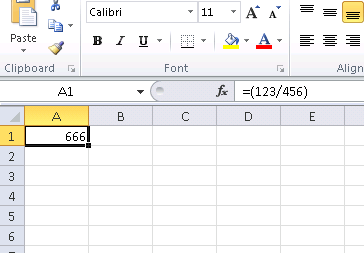
\includegraphics[scale=\NormalScale]{digging_into_code/Excel_prank.png}
\caption{\RU{Пранк сработал}\EN{The practical joke worked}}
\end{figure}

\RU{Если попробовать ту же версию Excel, только x64, то окажется что там инструкций \FDIV всего 12, 
причем нужная нам\EMDASH{}третья по счету.}
\EN{If we try the same Excel version, but in x64,
we will find only 12 \FDIV instructions there,
and the one we looking for is the third one.}

\begin{lstlisting}
tracer.exe -l:excel.exe bpx=excel.exe!BASE+0x1B7FCC,set(st0,666)
\end{lstlisting}

\myindex{x86!\Instructions!DIVSD}
\RU{Видимо, все дело в том, что много операций деления переменных типов \Tfloat и \Tdouble 
компилятор заменил на SSE-инструкции вроде \TT{DIVSD}, 
коих здесь теперь действительно много (\TT{DIVSD} присутствует в количестве 268 инструкций).}
\EN{It seems that a lot of division operations of \Tfloat and \Tdouble types, were replaced by the compiler with SSE instructions
like \TT{DIVSD} (\TT{DIVSD} is present 268 times in total).}

\chapter{\IFRU{Подозрительные паттерны кода}{Suspicious code patterns}}

\section{\IFRU{Инструкции XOR}{XOR instructions}}
\index{x86!\Instructions!XOR}

\IFRU{Инструкции вроде}{instructions like} \TT{XOR op, op} (\IFRU{например}{for example}, \TT{XOR EAX, EAX}) 
\IFRU{обычно используются для обнуления регистра,
однако, если операнды разные, то применяется операция именно}{are usually used for setting register value
to zero, but if operands are different,} \IT{\IFRU{исключающего или}{exclusive or}}\EN{ operation
is executed}.
\IFRU{Эта операция очень редко применяется в обычном программировании, но применяется очень часто в криптографии,
включая любительскую}{This operation is rare in common programming, but used often in cryptography,
including amateur}.
\IFRU{Особенно подозрительно, если второй операнд это большое число}{Especially suspicious case if the
second operand is big number}.
\IFRU{Это может указывать на шифрование, вычисление контрольной суммы, итд}
{This may points to encrypting/decrypting, checksum computing, etc}.\\
\\
\IFRU{Одно из исключений из этого наблюдения о котором стоит сказать, то, что генерация и проверка значения ``канарейки''
(\ref{subsec:BO_protection}) часто происходит используя инструкцию \XOR}
{One exception to this observation worth to note is ``canary'' (\ref{subsec:BO_protection}) generation and checking is often done using \XOR
instruction}. \\
\\
\index{AWK}
\IFRU{Этот AWK-скрипт можно использовать для обработки листингов (.lst) созданных \IDA{}}
{This AWK script can be used for processing \IDA{} listing (.lst) files}:

\begin{lstlisting}
gawk -e '$2=="xor" { tmp=substr($3, 0, length($3)-1); if (tmp!=$4) if($4!="esp") if ($4!="ebp") { print $1, $2, tmp, ",", $4 } }' filename.lst
\end{lstlisting}

\IFRU{Нельзя также забывать,
что если использовать подобный скрипт, то, возможно, он захватит и неверно дизассемблированный
код}{It is also worth to note that such script may also capture incorrectly disassembled code} 
(\ref{sec:incorrectly_disasmed_code}).

\section{\IFRU{Вручную написанный код на ассемблере}{Hand-written assembly code}}

\index{Function prologue}
\index{Function epilogue}
\index{x86!\Instructions!LOOP}
\index{x86!\Instructions!RCL}
\IFRU{Современные компиляторы не генерируют инструкции \TT{LOOP} и \TT{RCL}. 
С другой стороны, эти инструкции хорошо знакомы кодерам, предпочитающим писать прямо на ассемблере. 
Подобные инструкции отмечены как (M) в списке инструкций в приложении: \ref{sec:x86_instructions}.
Если такие инструкции встретились, можно сказать с какой-то вероятностью, что этот фрагмент кода написан вручную.}
{Modern compilers do not emit \TT{LOOP} and \TT{RCL} instructions.
On the other hand, these instructions are well-known to coders who like to code in straight assembly language.
If you spot these, it can be said, with a high probability, this fragment of code is hand-written.
Such instructions are marked as (M) in the instructions list in appendix: \ref{sec:x86_instructions}.}\\
\\
\IFRU{Также, пролог/эпилог функции обычно не встречается в ассемблерном коде, написанном вручную.}
{Also function prologue/epilogue is not commonly present in hand-written assembly copy.}\\
\\
\IFRU{Как правило, в вручную написанном коде, нет никакого четкого метода передачи аргументов в 
функцию}
{Commonly there is no fixed system in passing arguments into functions in the hand-written
code}.\\
\\
\IFRU{Пример из ядра}{Example from} Windows 2003\EN{ kernel} 
(\RU{файл }ntoskrnl.exe\EN{ file}):

\begin{lstlisting}
MultiplyTest proc near               ; CODE XREF: Get386Stepping
             xor     cx, cx
loc_620555:                          ; CODE XREF: MultiplyTest+E
             push    cx
             call    Multiply
             pop     cx
             jb      short locret_620563
             loop    loc_620555
             clc
locret_620563:                       ; CODE XREF: MultiplyTest+C
             retn
MultiplyTest endp

Multiply     proc near               ; CODE XREF: MultiplyTest+5
             mov     ecx, 81h
             mov     eax, 417A000h
             mul     ecx
             cmp     edx, 2
             stc
             jnz     short locret_62057F
             cmp     eax, 0FE7A000h
             stc
             jnz     short locret_62057F
             clc
locret_62057F:                       ; CODE XREF: Multiply+10
                                     ; Multiply+18
             retn
Multiply     endp
\end{lstlisting}

\IFRU{Действительно, если заглянуть в исходные коды}{Indeed, if we look into} 
\ac{WRK} v1.2\IFRU{, данный код можно найти в файле}{ source code, this code
can be found easily in the file} 
\IT{WRK-v1.2\textbackslash{}base\textbackslash{}ntos\textbackslash{}ke\textbackslash{}i386\textbackslash{}cpu.asm}.

\section{\IFRU{Использование magic numbers для трассировки}{Using magic numbers while tracing}}

\IFRU{Нередко бывает нужно узнать, как используется то или иное значение прочитанное из файла либо взятое из пакета
принятого по сети. Часто, ручное слежение за нужной переменной это трудный процесс. Один из простых методов (хотя и не
полностью надежный на 100\%) это использование вашей собственной \IT{magic number}.}
{Often, main goal is to get to know, how a value was read from file, or received via network, being used. 
Often, manual tracing of a value is very labouring task. One of the simple methods (however, not 100\% reliable) 
is to use your own \IT{magic number}.}

\IFRU{Это чем-то напоминает компьютерную томографию: пациенту перед сканированием вводят в кровь 
рентгеноконтрастный препарат, хорошо отсвечивающий в рентгеновских лучах. Известно как кровь нормального человека
расходится, например, по почкам, и если в этой крови будет препарат, то при томографии будет хорошо видно,
достаточно ли хорошо кровь расходится по почкам и нет ли там камней, например, и прочих образований.}
{This resembling X-ray computed tomography is some sense: radiocontrast agent is often injected into patient's blood,
which is used for improving visibility of internal structures in X-rays. For example, it is well known how blood of healthy man/woman
percolates in kidneys and if agent is in blood, it will be easily seen on tomography, how good and normal blood was percolating,
are there any stones or tumors.}

\IFRU{Мы можем взять 32-битное число вроде \IT{0x0badf00d}, либо чью-то дату рождения вроде \IT{0x11101979} 
и записать это, занимающее 4 байта число, в какое-либо место файла используемого исследуемой нами программой.}
{We can take a 32-bit number like \IT{0x0badf00d}, or someone's birth date like \IT{0x11101979}
and to write this, 4 byte holding number, to some point in file used by the program we investigate.}

\index{\GrepUsage}
\IFRU{Затем, при трассировки этой программы, в том числе, при помощи \tracer в режиме 
\IT{code coverage}, а затем при помощи
\IT{grep} или простого поиска по текстовому файлу с результатами трассировки, мы можем легко увидеть, в каких местах кода использовалось 
это значение, и как.}
{Then, while tracing this program, with \tracer in the \IT{code coverage} mode, and then, with the help of \IT{grep}
or just by searching in the text file (of tracing results), we can easily see, where the value was used and how.}

\IFRU{Пример результата работы \tracer в режиме \IT{cc}, к которому легко применить утилиту \IT{grep}}{Example 
of \IT{grepable} \tracer results in the \IT{cc} mode}:

\begin{lstlisting}
0x150bf66 (_kziaia+0x14), e=       1 [MOV EBX, [EBP+8]] [EBP+8]=0xf59c934 
0x150bf69 (_kziaia+0x17), e=       1 [MOV EDX, [69AEB08h]] [69AEB08h]=0 
0x150bf6f (_kziaia+0x1d), e=       1 [FS: MOV EAX, [2Ch]] 
0x150bf75 (_kziaia+0x23), e=       1 [MOV ECX, [EAX+EDX*4]] [EAX+EDX*4]=0xf1ac360 
0x150bf78 (_kziaia+0x26), e=       1 [MOV [EBP-4], ECX] ECX=0xf1ac360 
\end{lstlisting}

\IFRU{Это справедливо также и для сетевых пакетов.
Важно только чтобы наш \IT{magic number} был как можно более уникален и не присутствовал в самом коде.}
{This can be used for network packets as well.
It is important to be unique for \IT{magic number} and not to be present in the program's code.}

\newcommand{\DOSBOXURL}{\url{http://blog.yurichev.com/node/55}}

\index{DosBox}
\IFRU{Помимо \tracer, такой эмулятор MS-DOS как DosBox, в режиме heavydebug, может писать в отчет информацию обо всех
состояниях регистра на каждом шаге исполнения программы\footnote{См.также мой пост в блоге об этой возможности в 
DosBox: \DOSBOXURL{}}, так что этот метод может пригодиться и я для исследования программ под DOS.}{Aside of 
\tracer, DosBox (MS-DOS emulator) in heavydebug mode,
is able to write information about all register's states for each executed instruction of program to plain text file\footnote{See also my 
blog post about this DosBox feature: \DOSBOXURL{}}, so this method may be useful for DOS programs as well.}



\chapter{\RU{Прочее}\EN{Other things}}

\ac{RTTI}~(\ref{RTTI})-\RU{информация также может быть полезна для идентификации 
Си++-классов}\EN{data may be also useful for C++ classes identification}.

\chapter{\RU{Старые методы, тем не менее, интересные}
\EN{Old-school techniques, nevertheless, interesting to know}}

\subsection{\IFRU{Сравнение ``снимков'' памяти}{Memory ``snapshots'' comparing}}

\IFRU{Метод простого сравнения двух снимков памяти для поиска изменений часто применялся для взлома игр 
на 8-битных компьютерах и взлома файлов с записанными рекордными очками.}
{The method of simple two memory snapshots comparing in order to see changes, was often used to hack
8-bit computer games and hacking ``high score'' files.}

\IFRU{К примеру, если вы имеете загруженную игру на 8-битном компьютере (где самой памяти не очень много, но игра
занимает еще меньше), и вы знаете что сейчас у вас, условно, 100 пуль, вы можете сделать ``снимок'' всей
памяти и сохранить где-то. Затем просто стреляете куда угодно, у вас станет 99 пуль, сделать второй ``снимок'',
и затем сравнить эти два снимка: где-то наверняка должен быть байт, который в начале был 100, а затем стал 99.}
{For example, if you got some loaded game on 8-bit computer (it's not much memory on these, but game is usually
consumes even less memory) and you know that you have now, let's say, 100 bullets, you can do a ``snapshot''
of all memory and save it to some place. Then shoot somewhere, bullet count now 99, do second ``snapshot''
and then compare both: somewhere should be a byte which was 100 in the beginning and now it's 99.}
\IFRU{Если учесть что игры на тех маломощных домашних компьютерах обычно были написанны на ассемблере и подобные
переменные там были глобальные, то можно с уверенностью сказать, какой адрес в памяти всегда отвечает за количество
пуль. Если поискать в дизассемблированном коде игры все обращения по этому адресу, несложно найти код,
отвечающий за уменьшение пуль и записать туда инструкцию \NOP\footnote{``no operation'', холостая инструкция} 
или несколько \NOP-в, так мы получим игру в которой у игрока всегда будет 100 пуль, например.}
{Considering a fact that these 8-bit games were often written in assembler and such variables were global,
it can be said for sure, which address in memory holding bullets count. If to search all references to that
address in disassembled game code, it's not very hard to find a piece of code decrementing bullets count,
write \NOP instruction\footnote{``no operation'', idle operation} there, or couple of \NOP{}-s, 
we'll have a game with 100 (for example) bullets forever.}
\IFRU{А так как игры на тех домашних 8-битных 
компьютерах всегда загружались по одним и тем же адресам, и версий одной игры редко когда было больше одной,
то геймеры-энтузиасты знали, по какому адресу (используя инструкцию языка BASIC \IT{POKE}\footnote{инструкция языка BASIC записывающая байт по определенному адресу}) что записать после загрузки
игры, чтобы хакнуть её. Это привело к появлению списков ``читов'' состоящих из инструкций \IT{POKE}, публикуемых
в журналах посвященным 8-битным играм. См.также:}{Games on these 8-bit computers was usually loaded on the same
address, also, there were no much different versions of each game (usually, just one version all have),
enthusiastic gamers knew, which byte should be written (using BASIC instruction \IT{POKE}\footnote{BASIC language instruction writting byte on specific address}) to which address in
order to hack it. This led to ``cheat'' lists containing of \IT{POKE} instructions published in magazines related to
8-bit games. See also:} \url{http://en.wikipedia.org/wiki/PEEK\_and\_POKE}.

\IFRU{Точно также легко модифицировать файлы с сохраненными рекордами, кто сколько очков набрал, впрочем, это может
сработать не только с 8-битными играми. Нужно заметить, какой у вас сейчас рекорд и где-то сохранить файл
с очками. Затем, когда очков станет другое количество, просто сравнить два файла, можно даже
DOS-утилитой FC\footnote{утилита MS-DOS для сравнения двух файлов побайтово} (файлы рекордов, часто, бинарные).}
{The same story about modifying ``high score'' files, this may work not only with 8-bit games. Let's notice 
your score count and save the file somewhere. When ``high score'' count will be different, just compare two files,
it can be even done with DOS-utility FC\footnote{MS-DOS utility for binary files comparing} (``high score'' files
are often in binary form).}
\IFRU{Где-то будут отличаться несколько байт, и легко будет увидеть, какие именно отвечают за количество очков. 
Впрочем, разработчики игр осведомлены о таких хитростях и могут защититься от этого.}
{There will be some place where couple of bytes will be different and it will be easy to see which ones are
holding score number.
However, game developers are aware of such tricks and may protect against it.}

% FIXME: пример с какой-то простой игрушкой?



\chapter{\IFRU{Специфичное для ОС}{OS-specific}}
% sections here
\section{\IFRU{Форматы файлов}{File formats}}
\subsection{Win32 PE}
\label{win32_pe}

\acs{PE} \IFRU{это формат исполняемых файлов, принятый в Windows}{is a executable file format used in
Windows}.

\IFRU{Разница между .exe, .dll, и .sys в том, что у .exe и .sys обычно нет экспортов, только импорты}
{The difference between .exe, .dll and .sys is that .exe and .sys usually does not have exports, only imports}.

\index{OEP}
\IFRU{У \ac{DLL}, как и у всех PE-файлов, есть точка входа (\ac{OEP})
(там располагается ф-ция DllMain()), но обычно эта ф-ция ничего не делает.}
{A \ac{DLL}, just as any other PE-file, has entry point (\ac{OEP}) (the function DllMain() is located at it) 
but usually this function does nothing.}

.sys \IFRU{это обычно драйвера устройств}{is usually device driver}.

\IFRU{Для драйверов, Windows требует чтобы контрольная сумма в PE-файле была проставлена
и была верной}
{As of drivers, Windows require the checksum is present in PE-file and must be correct}
\footnote{\IFRU{Например}{For example}, Hiew(\ref{Hiew}) \IFRU{умеет её подсчитывать}{can calculate it}}.

\index{Windows!Windows Vista}
\IFRU{А начиная с}{Starting at} Windows Vista, 
\IFRU{PE-файлы-драйвера должны быть также подписаны при помощи электронной подписи, 
иначе они не будут загружаться.}
{driver PE-files must be also signed by digital signature. It will fail to load without signature.}

\index{MS-DOS}
\IFRU{В начале всякого PE-файла есть крохотная DOS-программа,
выводящая на консоль сообщение вроде}{Any PE-file begins with tiny DOS-program, printing a
message like} ``This program cannot be run in DOS mode.'' --- 
\IFRU{если запустить эту программу в DOS либо Windows 3.1, выведется это сообщение}
{if to run this program in DOS or Windows 3.1, this message will be printed}.

\subsubsection{\IFRU{Терминология}{Terminology}}

\begin{itemize}
\item
\IFRU{Модуль}{Module} --- \IFRU{это отдельный файл}{is a separate file}, .exe \OrENRU .dll.

\item
\IFRU{Процесс}{Process} --- \IFRU{это некая загруженная в память и работающая программа}{a program
loaded into memory and running}.
\IFRU{Как правило состоит из одного .exe-файла и массы .dll-файлов}{Commonly consisting of 
one .exe-file and bunch of .dll-files}.

\item
\IFRU{Память процесса}{Process memory} --- \IFRU{память с которой работает процесс}{the memory a process
works with}.
\IFRU{У каждого процесса --- своя}{Each process has its own}.
\IFRU{Там обычно имеются загруженные модули, память стека, \glslink{heap}{кучи}, и т.д}{There can usually be 
loaded modules, memory of the stack, \gls{heap}(s), etc}.

\item
\index{VA}
\ac{VA} --- \IFRU{это адрес, который будет использоваться в самой программе}{is address which will
be used in program}.

\item
\index{\IFRU{Базовый адрес}{Base address}}
\IFRU{Базовый адрес}{Base address}\EMDASH{}\IFRU{это адрес, по которому модуль будет загружен 
в пространство процесса}{is the address within a process memory at which a module will be loaded}.

\item
\index{RVA}
\ac{RVA}\EMDASH{}\IFRU{это}{is a} \ac{VA}-\IFRU{адрес минус базовый адрес}{address minus base address}.
\IFRU{Многие адреса в таблицах PE-файла используют именно}{Many addresses in PE-file tables
uses exactly} \ac{RVA}-\IFRU{адреса}{addresses}.

%\item
%Data directory\EMDASH{}...

\item 
\index{IAT}
\ac{IAT}\EMDASH{}\IFRU{массив адресов импортированных символов}{an array of addresses of imported symbols}
\footnote{\cite{Pietrek1}}. 
\IFRU{Иногда, директория}{Sometimes, a} \TT{IMAGE\_DIRECTORY\_ENTRY\_IAT} \IFRU{указывает на}
{data directory is points to the} \ac{IAT}. 
\label{IDA_idata}
\IFRU{Важно отметить, что}{It is worth to note that} \ac{IDA} (\IFRU{по крайней мере}{as of} 6.1) 
\IFRU{может выделить псевдо-секцию с именем}{may allocate a pseudo-section named} \TT{.idata} \ForENRU
\ac{IAT}, \IFRU{даже если}{even if} \ac{IAT} \IFRU{является частью совсем другой секции}
{is a part of another section}!

\item 
\index{INT}
\ac{INT}\EMDASH{}\IFRU{массив имен символов для импортирования}
{an array of names of symbols to be imported}\footnote{\cite{Pietrek1}}.
\end{itemize}

\subsubsection{\IFRU{Базовый адрес}{Base address}}

\IFRU{Дело в том, что несколько авторов модулей могут готовить DLL-файлы для других, и нет возможности договориться о том, какие адреса и кому будут отведены.}
{The fact is that several module authors may prepare DLL-files for others and there is no possibility
to reach agreement, which addresses will be assigned to whose modules.}

\IFRU{Поэтому, если у двух необходимых для загрузки процесса DLL одинаковые базовые адреса,
одна из них будет загружена по этому базовому адресу, 
а вторая ~--- по другому свободному месту в памяти процесса, и все виртуальные адреса
во второй DLL будут скорректированы.}
{So that is why if two necessary for process loading DLLs has the same base addresses,
one of which will be loaded at this base address, and another~---at the other spare space in process memory,
and each virtual addresses in the second DLL will be corrected.} \\
\\
\IFRU{Очень часто линкер в}{Often, linker in} \ac{MSVC} \IFRU{генерирует .exe-файлы с базовым адресом}
{generates an .exe-files with the base address} \TT{0x400000},
\IFRU{и с секцией кода начинающейся с}{and with the code section started at} \TT{0x401000}.
\IFRU{Это значит, что}{This mean} \ac{RVA} \IFRU{начала секции кода ~---}{of code section begin is} \TT{0x1000}.
\IFRU{А \ac{DLL} часто генерируются этим линкером с базовым адресом}
{DLLs are often generated by this linked with the base address} \TT{0x10000000}
\footnote{\IFRU{Это можно изменять опцией /BASE в линкере}{This can be changed by /BASE linker option}}.

\index{ASLR}
\IFRU{Помимо всего прочего, есть еще одна причина намеренно загружать модули по разным адресам, а точнее, 
по случайным}
{There is also another reason to load modules at various base addresses, rather at random ones}.

\IFRU{Это}{It is} \ac{ASLR}
\footnote{\IFRU{\url{https://ru.wikipedia.org/wiki/Address_Space_Layout_Randomization}}
{\url{https://en.wikipedia.org/wiki/Address_space_layout_randomization}}}.

\index{shellcode}
\IFRU{Дело в том, что некий шеллкод, пытающийся исполниться на зараженной системе, 
должен вызывать какие-то системные ф-ции}{The fact is that a shellcode trying to be executed on a compromised
system must call a system functions}.

\IFRU{И в старых}{In older} \ac{OS} (\IFRU{в линейке \gls{Windows NT}: до}{in \gls{Windows NT} line: before} Windows Vista),
\IFRU{системные}{system} DLL (\IFRU{такие как}{like} kernel32.dll, user32.dll) \IFRU{загружались все время
по одним и тем же адресам}{were always loaded at the known addresses}, 
\IFRU{а если еще и вспомнить, что версии этих DLL редко менялись}{and also if to recall
that its versions were rarely changed}, \IFRU{то адреса отдельных
ф-ций, можно сказать, фиксированы и шеллкод может вызывать их напрямую}{an addresses of functions were
fixed and shellcode can call it directly}.

\IFRU{Чтобы избежать этого, методика}{In order to avoid this,} \ac{ASLR}
\IFRU{загружает и вашу программу, и все модули ей необходимые, по случайным адресам, разным при каждом запуске}
{method loads your program and all modules it needs at random base addresses, each time different}.

\IFRU{В PE-файлах, поддержка \ac{ASLR} отмечается выставлением флага}
{\ac{ASLR} support is denoted in PE-file by setting the flag} \\
\TT{IMAGE\_DLL\_CHARACTERISTICS\_DYNAMIC\_BASE} \cite{Russinovich}.

\subsubsection{Subsystem}

\IFRU{Имеется также поле \IT{subsystem}, обычно это}{There is also \IT{subsystem} field, usually it is}
native (.sys-\IFRU{драйвер}{driver}), 
console (\IFRU{консольное приложение}{console application}) \OrENRU 
\ac{GUI} (\IFRU{не консольное}{non-console}).

\subsubsection{\IFRU{Версия ОС}{OS version}}

\IFRU{В PE-файле имеется минимальный номер версии Windows, необходимый для загрузки модуля.}
{A PE-file also has minimal Windows version needed in order to load it.}
\IFRU{Соответствие номеров версий в файле и кодовых наименований Windows, можно посмотреть}
{The table of version numbers stored in PE-file and corresponding Windows codenames is}
\href{https://en.wikipedia.org/wiki/Windows_NT#Releases}{\IFRU{здесь}{here}}.

\index{Windows!Windows NT4}
\index{Windows!Windows 2000}
\IFRU{Например}{For example}, \ac{MSVC} 2005 \IFRU{еще компилирует .exe-файлы запускающиеся на}{compiles
.exe-files running on} Windows NT4 (\IFRU{версия}{version} 4.00),
\IFRU{а вот}{but} \ac{MSVC} 2008 \IFRU{уже нет}{is not} 
(\IFRU{генерируемые файлы имеют версию}{files generated has version} 5.00, 
\IFRU{для запуска необходима как минимум Windows 2000}{at least Windows 2000 is needed to run them}).

\index{Windows!Windows XP}
\ac{MSVC} 2012 \IFRU{по умолчанию генерирует .exe-файлы версии}{by default generates .exe-files of version} 6.00, 
\IFRU{для запуска нужна как минимум Windows Vista}{targeting at least Windows Vista}, \IFRU{хотя}{however, by} 
\href{http://blogs.msdn.com/b/vcblog/archive/2012/10/08/10357555.aspx}{\IFRU{изменив настройки компиляции}
{by changing compiler's options}}, 
\IFRU{можно заставить генерировать и под Windows XP}{it is possible to force it to compile for Windows XP}.

\subsubsection{\IFRU{Секции}{Sections}}

\IFRU{Разделение на секции присутствует, по-видимому, во всех форматах исполняемых файлов}{Division by sections,
as it seems, are present in all executable file formats}.

\IFRU{Сделано это для того, чтобы отделить код от данных, а данные ~--- от константных данных.}
{It is done in order to separate code from data, and data~---from constant data.}

\begin{itemize}
\item
\IFRU{На секции кода будет стоять флаг}{There will be flag} 
\IT{IMAGE\_SCN\_CNT\_CODE} \OrENRU \IT{IMAGE\_SCN\_MEM\_EXECUTE}\EN{ on code section}\EMDASH\IFRU{это исполняемый код}{this is executable code}.

\item
\IFRU{На секции данных}{On data section}\EMDASH\IFRU{флаги }{}\IT{IMAGE\_SCN\_CNT\_INITIALIZED\_DATA}, 
\IT{IMAGE\_SCN\_MEM\_READ} \AndENRU \IT{IMAGE\_SCN\_MEM\_WRITE}\EN{ flags}.

\item
\IFRU{На пустой секции с неинициализированными данными}{On an empty section with uninitialized 
data}\EMDASH\IT{IMAGE\_SCN\_CNT\_UNINITIALIZED\_DATA}, \IT{IMAGE\_SCN\_MEM\_READ} \AndENRU \IT{IMAGE\_SCN\_MEM\_WRITE}.

\item
\IFRU{А на секции с константными данными, то есть, защищенными от записи}{On a constant data section, in other words,
protected from writing}, \IFRU{могут быть флаги}
{there are may be flags} \\
\IT{IMAGE\_SCN\_CNT\_INITIALIZED\_DATA} \AndENRU \IT{IMAGE\_SCN\_MEM\_READ} \IFRU{без}{without} \IT{IMAGE\_SCN\_MEM\_WRITE}. 
\IFRU{Если попытаться записать что-то в эту секцию, процесс упадет}{A process will crash if it would try to write to this
section}.
\end{itemize}

\IFRU{В PE-файле можно задавать название для секции, но это не важно}{Each section in PE-file may have a name, however,
it is not very important}.
\IFRU{Часто (но не всегда)}{Often (but not always)} \IFRU{секция кода называется}{code section have the name} \TT{.text}, 
\index{TLS}
\index{BSS}
\IFRU{секция данных}{data section} --- \TT{.data}, \IFRU{константных данных}{constant data section} --- \TT{.rdata} 
\IT{(readable data)}.
\IFRU{Еще популярные имена секций}{Other popular section names are}: 

\index{MIPS}
\begin{itemize}
\item \TT{.idata}\EMDASH{}\IFRU{секция импортов}{imports section}.
\ac{IDA} \IFRU{может создавать псевдо-секцию с этим же именем}
{may create pseudo-section named like this}: \ref{IDA_idata}.
\item \TT{.edata}\EMDASH{}\IFRU{секция экспортов}{exports section}
\item \TT{.pdata}\EMDASH{}\IFRU{секция содержащая информацию об исключениях в Windows NT для MIPS, \ac{IA64} и x64}
{section containing all information about exceptions in Windows NT for MIPS, \ac{IA64} and x64}: \ref{SEH_win64}
\item \TT{.reloc}\EMDASH{}\IFRU{секция релоков}{relocs section}
\item \TT{.bss}\EMDASH{}\IFRU{неинициализированные данные}{uninitialized data (\ac{BSS})}
\item \TT{.tls}\EMDASH{}thread local storage (\ac{TLS})
\item \TT{.rsrc}\EMDASH{}\IFRU{ресурсы}{resources}
\item \TT{.CRT}\EMDASH{}\IFRU{может присутствует в бинарных файлах скомпилированных очень старыми версиями MSVC}
{may present in binary files compiled by very old MSVC versions}
\end{itemize}

\IFRU{Запаковщики/зашифровщики PE-файлов часто затирают имена секций, или меняют на свои}
{PE-file packers/encryptors are often garble section names or replacing names to their own}.

\IFRU{В \ac{MSVC} можно объявлять данные в произвольно названной секции}
{\ac{MSVC} allows to declare data in arbitrarily named section}
\footnote{\url{http://msdn.microsoft.com/en-us/library/windows/desktop/cc307397.aspx}}.

\IFRU{Некоторые компиляторы и линкеры могут добавлять также секцию с отладочными символами 
и вообще отладочной информацией}
{Some compilers and linkers can add a section with debugging symbols and other debugging information}
(\IFRU{например,}{e.g.} MinGW).
\index{PDB}
\IFRU{Хотя это не так в современных версиях}{However it is not so in modern versions of} \ac{MSVC} 
(\IFRU{там принято отладочную информацию сохранять в отдельных PDB-файлах}
{a separate PDB-files are used there for this purpose}).

\IFRU{Вот как секция описывается в файле}{That is how section described in the file}:

\begin{lstlisting}
typedef struct _IMAGE_SECTION_HEADER {
  BYTE  Name[IMAGE_SIZEOF_SHORT_NAME];
  union {
    DWORD PhysicalAddress;
    DWORD VirtualSize;
  } Misc;
  DWORD VirtualAddress;
  DWORD SizeOfRawData;
  DWORD PointerToRawData;
  DWORD PointerToRelocations;
  DWORD PointerToLinenumbers;
  WORD  NumberOfRelocations;
  WORD  NumberOfLinenumbers;
  DWORD Characteristics;
} IMAGE_SECTION_HEADER, *PIMAGE_SECTION_HEADER;
\end{lstlisting}
\footnote{\url{http://msdn.microsoft.com/en-us/library/windows/desktop/ms680341(v=vs.85).aspx}}

\index{Hiew}
\IFRU{Еще немного терминологии}{A word about terminology}:
\IT{PointerToRawData} \IFRU{называется}{it called} ``Offset''
\AndENRU \IT{VirtualAddress} \IFRU{называется}{is called} ``RVA'' \InENRU Hiew.

\subsubsection{\IFRU{Релоки}{Relocations (relocs)}}

\IFRU{Так же известны как FIXUP-ы}{\ac{AKA} FIXUP-s} (\IFRU{по крайней мере в}{at least in} Hiew).

\IFRU{Это также присутствует почти во всех форматах загружаемых и исполняемых файлов}
{This is also present in almost all executable file formats}
\footnote{\IFRU{Даже .exe-файлы в}{Even .exe-files in} MS-DOS}.

\IFRU{Как видно, модули могут загружаться по другим базовым адресам,
но как же тогда работать с глобальными переменными, например?}
{Obviously, modules can be loaded on various base addresses,
but how to deal with e.g. global variables?}
\IFRU{Ведь нужно обращаться к ним по адресу}{They must be accessed by an address}.
\IFRU{Одно из решений это}{One solution is} \PICcode(\ref{sec:PIC}).
\IFRU{Но это далеко не всегда удобно}{But it is not always suitable}.

\IFRU{Поэтому имеется таблица релоков. 
Там просто перечислены адреса мест в модуле подлежащими коррекции при загрузке
по другому базовому адресу.}
{That is why relocations table is present.
The addresses of points needs to be corrected in case of loading on another base address 
are just enumerated in the table.}

\IFRU{Например, по}{For example, there is a global variable at the address}
\TT{0x410000} 
\IFRU{лежит некая глобальная переменная, и вот как обеспечивается её чтение}
{and this is how it is accessed}:

\begin{lstlisting}
A1 00 00 41 00         mov         eax,[000410000]
\end{lstlisting}

\IFRU{Базовый адрес модуля}{Base address of module is} \TT{0x400000},
\RU{а }\ac{RVA} \IFRU{глобальной переменной}{of global variable is} \TT{0x10000}.

\IFRU{Если загружать модуль по базовому адресу}{If the module is loading on the base address}
\TT{0x500000}, \IFRU{нужно чтобы адрес этой переменной в этой инструкции стал}{the factual address
of the global variable must be} \TT{0x510000}.

\index{x86!\Instructions!MOV}
\IFRU{Как видно, адрес переменной закодирован в самой инструкции}
{As we can see, address of variable is encoded in the instruction} \TT{MOV}, 
\IFRU{после байта}{after the byte} \TT{0xA1}.

\IFRU{Поэтому адрес четырех байт}{That is why address of 4 bytes}, \IFRU{после}{after} \TT{0xA1},
\IFRU{записывается в таблицу релоков}{is written into relocs table}.

\IFRU{Если модуль загружается по другому базовому адресу},
\IFRU{загрузчик \ac{OS} обходит все адреса в таблице}{\ac{OS}-loader enumerates all addresses in table}, 
\IFRU{находит каждое 32-битное слово по этому адресу}
{finds each 32-bit word the address points on},
\IFRU{отнимает от него настоящий, оригинальный базовый адрес}{subtracts real, original base address of it}
(\IFRU{в итоге получается}{we getting} \ac{RVA}\EN{ here}),
\IFRU{и прибавляет к нему новый базовый адрес}{and adds new base address to it}.

\IFRU{А если модуль загружается по своему оригинальному базовому адресу, ничего не происходит}
{If module is loading on original base address, nothing happens}.

\IFRU{Так можно обходиться со всеми глобальными переменными}
{All global variables may be treated like that}.

\IFRU{Релоки могут быть разных типов}{Relocs may have various types}, 
\IFRU{однако в Windows для x86-процессоров, тип обычно}
{however, in Windows, for x86 processors, the type is usually} \\
\IT{IMAGE\_REL\_BASED\_HIGHLOW}.

\index{Hiew}
\IFRU{Кстати, релоки маркируются темным в Hiew, например}
{By the way, relocs are darkened in Hiew, for example} \figname \ref{fig:scanf_ex3_hiew_1}.

\subsubsection{\IFRU{Экспорты и импорты}{Exports and imports}}

\label{PE_exports_imports}
\IFRU{Как известно}{As all we know}, 
\IFRU{любая исполняемая программа должна как-то пользоваться сервисами \ac{OS} и прочими DLL-библиотеками}
{any executable program must use \ac{OS} services and other DLL-libraries somehow}.

\IFRU{Можно сказать, что нужно связывать функции из одного модуля (обычно DLL) и места их вызовов в 
другом модуле (.exe-файл или другая DLL)}
{It can be said, functions from one module (usually DLL) must be connected somehow to a points of their
calls in other module (.exe-file or another DLL)}.

\IFRU{Для этого, у каждой DLL есть ``экспорты'', это таблица ф-ций плюс их адреса в модуле}
{Each DLL has ``exports'' for this, this is table of functions plus its addresses in a module}.

\IFRU{А у .exe-файла, либо DLL, есть ``импорты'', это таблица ф-ций требующихся для исполнения 
включая список имен DLL-файлов}
{Each .exe-file or DLL has ``imports'', this is a table of functions it needs for execution including
list of DLL filenames}.

\IFRU{Загрузчик \ac{OS}, после загрузки основного .exe-файла, проходит по таблице импортов:
загружает дополнительные DLL-файлы, 
находит имена ф-ций среди экспортов в DLL и прописывает их адреса в \ac{IAT} в головном .exe-модуле}
{After loading main .exe-file, \ac{OS}-loader, processes imports table: 
it loads additional DLL-files, finds function names
among DLL exports and writes their addresses down in an \ac{IAT} of main .exe-module}.

\index{Ordinal}
\IFRU{Как видно, во время загрузки, загрузчику нужно много сравнивать одни имена ф-ций с другими,
а сравнение строк ~--- это не очень быстрая процедура, так что,
имеется также поддержка ``ординалов'' или 
``hint''-ов, это когда в таблице импортов проставлены номера ф-ций вместо их имен}
{As we can notice, during loading, loader must compare a lot of function names, but strings comparison is not a very
fast procedure, so, there is a support of ``ordinals'' or ``hints'',
that is a function numbers stored in the table instead of their names}.

\IFRU{Так их быстрее находить в загружаемой DLL}
{That is how they can be located faster in loading DLL}.
\IFRU{В таблице экспортов ординалы присутствуют всегда}{Ordinals are always present in ``export'' table}.

\index{MFC}
\IFRU{К примеру}{For example}, \IFRU{программы использующие библиотеки}{program using} 
\ac{MFC}\IFRU{, обычно загружают mfc*.dll по ординалам}{ library usually loads mfc*.dll by ordinals},
\IFRU{и в таких программах, в \ac{INT}, нет имен ф-ций \ac{MFC}}
{and in such programs there are no \ac{MFC} function names in \ac{INT}}.

\IFRU{При загрузке такой программы в \IDA, она спросит у вас путь к файлу mfc*.dll,
чтобы установить имена ф-ций}{While loading such program in \IDA, it will asks for a path to mfs*.dll files,
in order to determine function names}.
\IFRU{Если в \IDA не указать путь к этой DLL, то вместо имен ф-ций будет что-то вроде}
{If not to tell \IDA path to this DLL, they will look like}
\IT{mfc80\_123}\EN{ instead of function names}.

\paragraph{\IFRU{Секция импортов}{Imports section}}

\IFRU{Под таблицу импортов и всё что с ней связано иногда отводится отдельная секция 
(с названием вроде \TT{.idata}),
но это не обязательно}
{Often a separate section is allocated for imports table and everything related to it (with name like \TT{.idata}),
however, it is not a strict rule}.

\IFRU{Импорты ~--- это запутанная тема еще и из-за терминологической путаницы. Попробуем собрать всё в одно место.}
{Imports is also confusing subject because of terminological mess. Let's try to collect all information in one place.}

\begin{figure}[H]
\centering
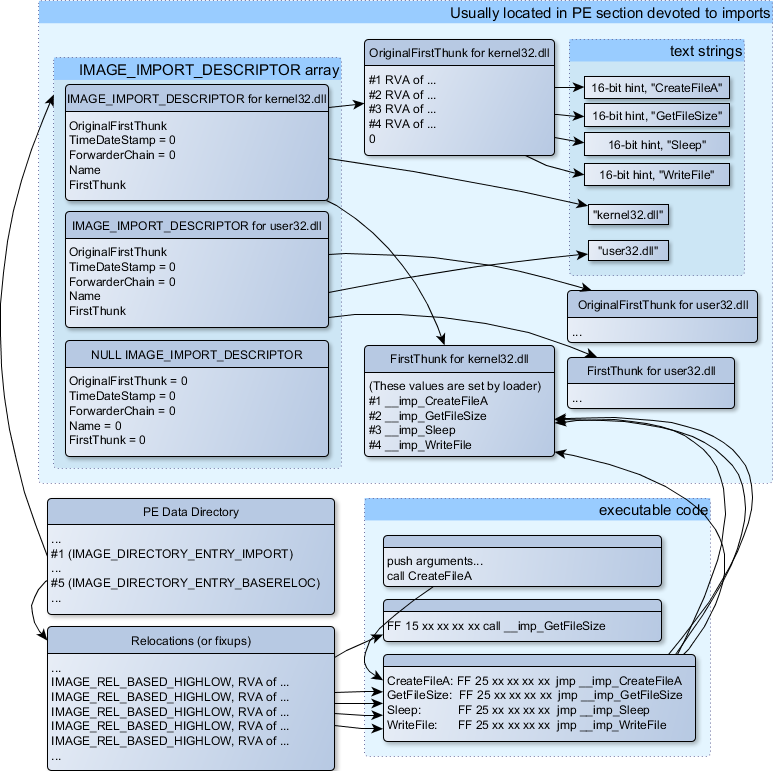
\includegraphics[scale=0.66]{OS-specific/PE/unnamed0.png}
\caption{\IFRU{схема, объединяющая все структуры в PE-файлы, связанные с импортами}
{The scheme, uniting all PE-file structures related to imports}}
\end{figure}

\IFRU{Самая главная структура ~--- это массив}{Main structure is the array of} \IT{IMAGE\_IMPORT\_DESCRIPTOR}.
\IFRU{Каждый элемент на каждую импортируемую DLL}{Each element for each DLL being imported}.

\IFRU{У каждого элемента есть}{Each element holds} \ac{RVA}-\IFRU{адрес}{address} 
\IFRU{текстовой строки (имя DLL)}{of text string (DLL name)} (\IT{Name}).

\IT{OriginalFirstThink} \IFRU{это}{is a} \ac{RVA}-\IFRU{адрес таблицы \ac{INT}}{address of \ac{INT} table}. 
\IFRU{Это массив}{This is array of} 
\ac{RVA}-\IFRU{адресов}{addresses},
\IFRU{каждый из которых указывает на текстовую строку где записано имя ф-ции}
{each of which points to the text string with function name}. 
\IFRU{Каждую строку предваряет 16-битное число}{Each string is prefixed by 16-bit integer} 
(``hint'')\EMDASH\IFRU{``ординал'' ф-ции}{``ordinal'' of function}.

\IFRU{Если при загрузке удается найти ф-цию по ординалу, тогда сравнение текстовых строк не будет происходить.
Массив оканчивается нулем}{While loading, if it is possible to find function by ordinal,
then strings comparison will not occur. Array is terminated by zero}.
\IFRU{Есть также указатель на таблицу \ac{IAT} с названием}
{There is also a pointer to the \ac{IAT} table with a name} \IT{FirstThunk},
\IFRU{это просто}{it is just} \ac{RVA}-\IFRU{адрес}{address} 
\IFRU{места, где загрузчик будет проставлять адреса найденных ф-ций}{of the place where loader will
write addresses of functions resolved}.

\IFRU{Места где загрузчик проставляет адреса, \IDA именует их так}{The points where
loader writes addresses, \IDA marks like}: \IT{\_\_imp\_CreateFileA}, \IFRU{и т.д}{etc}.

\IFRU{Есть по крайней мере два способа использовать адреса, проставленные загрузчиком}
{There are at least two ways to use addresses written by loader}.

\begin{itemize}
\index{x86!\Instructions!CALL}
\item
\IFRU{В коде будут просто инструкции вроде}{The code will have instructions like} 
\IT{call \_\_imp\_CreateFileA}, 
\IFRU{а так как, поле с адресом импортируемой ф-ции это как бы глобальная переменная}
{and since the field with the address of function imported is a global variable in some sense}, 
\IFRU{то в таблице релоков добавляется адрес (плюс 1 или 2) в инструкции \IT{call}}
{the address of \IT{call} instruction (plus 1 or 2) will be added to relocs table},
\IFRU{на случай если модуль будет загружен по другому базовому адресу}
{for the case if module will be loaded on different base address}.

\IFRU{Но как видно, это приводит к увеличению таблицы релоков}{But, obviously, this may enlarge
relocs table significantly}.
\IFRU{Ведь вызовов импортируемой ф-ции у вас в модуле может быть очень много}
{Because there are might be a lot of calls to imported functions in the module}.
\IFRU{К тому же, чем больше таблица релоков, тем дольше загрузка}
{Furthermore, large relocs table slowing down the process of module loading}.

\index{x86!\Instructions!JMP}
\index{thunk-\IFRU{функции}{functions}}
\item
\IFRU{На каждую импортируемую ф-цию выделяется только один переход на импортируемую ф-цию используя
инструкцию \JMP плюс релок на эту инструкцию}
{For each imported function, there is only one jump allocated, using \JMP instruction 
plus reloc to this instruction}.
\IFRU{Такие места-``переходники'' называются также ``thunk''-ами}{Such points are also called ``thunks''}.
\IFRU{А все вызовы импортируемой ф-ции это просто инструкция \CALL на соответствующий ``thunk''}
{All calls to the imported functions are just \CALL instructions to the corresponding ``thunk''}.
\IFRU{В данном случае, дополнительные релоки не нужны, потому что эти CALL-ы имеют относительный адрес,
и корректировать их не надо}{In this case, additional relocs are not necessary because these CALL-s
has relative addresses, they are not to be corrected}.
\end{itemize}

\IFRU{Оба этих два метода могут комбинироваться}{Both of these methods can be combined}.
\IFRU{Вероятно, линкер создает отдельный ``thunk'', если вызовов слишком много, но по умолчанию --- не создает}
{Apparently, linker creates individual ``thunk'' if there are too many calls to the functions,
but by default it is not to be created}. \\
\\
\IFRU{Кстати, массив адресов ф-ций, на который указывает FirstThunk,
не обязательно может быть в секции \ac{IAT}}{By the way, an array of function addresses to which FirstThunk is
pointing is not necessary to be located in \ac{IAT} section}.
\IFRU{К примеру, я написал утилиту}{For example, I once wrote the}
PE\_add\_import\footnote{\url{http://yurichev.com/PE_add_imports.html}} 
\IFRU{для добавления импорта в уже существующий .exe-файл}{utility for adding import to an existing .exe-file}.
\IFRU{Раньше, в прошлых версиях утилиты, на месте ф-ции, вместо которой вы хотите подставить вызов в другую DLL,
моя утилита вписывала такой код}{Some time earlier, in the previous versions of the utility, 
at the place of the function you want to substitute by call to another DLL,
the following code my utility writed}:

\begin{lstlisting}
MOV EAX, [yourdll.dll!function]
JMP EAX
\end{lstlisting}

\IFRU{При этом, FirstThunk указывает прямо на первую инструкцию.
Иными словами, загрузчик, загружая yourdll.dll, 
прописывает адрес ф-ции \IT{function} прямо в коде.}
{FirstThunk points to the first instruction. In other words, while loading yourdll.dll,
loader writes address of the \IT{function} function right in the code.}

\IFRU{Надо также отметить что обычно секция кода защищена от записи}
{It also worth noting a
code section is usually write-protected}, \IFRU{так что, моя утилита
добавляет флаг}{so my utility adds} \IT{IMAGE\_SCN\_MEM\_WRITE} 
\IFRU{для секции кода. Иначе при загрузке такой программы, она упадет с ошибкой}
{flag for code section. Otherwise, the program will crash while loading with the error code}
5 (access denied). \\
\\
\IFRU{Может возникнуть вопрос: а что если я поставляю программу с набором DLL,
которые никогда не будут меняться, может как-то можно ускорить процесс загрузки?}
{One might ask: what if I supply a program with the DLL files set which are not supposed to change,
is it possible to speed up loading process?}

\IFRU{Да, можно прописать адреса импортируемых ф-ций в массивы FirstThunk заранее}
{Yes, it is possible to write addresses of the functions to be imported into FirstThunk arrays in advance}.
\IFRU{Для этого в структуре}{The \IT{Timestamp} field is present in the}
\IT{IMAGE\_IMPORT\_DESCRIPTOR} \IFRU{имеется поле \IT{Timestamp}}{structure}.
\IFRU{И если там присутствует какое-то значение, то загрузчик сверяет это значение с датой-временем DLL-файла}
{If a value is present there, then loader compare this value with date-time of the DLL file}.
\IFRU{И если они равны, то загрузчик больше ничего не делает, и загрузка будет происходить быстрее}
{If the values are equal to each other, then the loader is not do anything, and loading process will be faster}.
\IFRU{Это называется}{This is what called} ``old-style binding''
\footnote{\url{http://blogs.msdn.com/b/oldnewthing/archive/2010/03/18/9980802.aspx}.
\IFRU{Существует также}{There is also} ``new-style binding'',
\IFRU{про него напишу позже}{I will write about it in future}}.
\index{BIND.EXE}
\IFRU{В Windows SDK для этого имеется утилита BIND.EXE}
{There is the BIND.EXE utility in Windows SDK for this}.
\IFRU{Для ускорения загрузки вашей программы}{For speeding up of loading of your program}, 
Matt Pietrek \InENRU \cite{Pietrek1}, \IFRU{предлагает делать binding сразу после инсталляции
вашей программы на компьютере конечного пользователя}{offers to do binding shortly after your program
installation on the computer of the end user}. \\
\\
\IFRU{Запаковщики/зашифровщики PE-файлов могут также сжимать/шифровать таблицу импортов}
{PE-files packers/encryptors may also compress/encrypt imports table}.
\IFRU{В этом случае, загрузчик Windows, конечно же, не загрузит все нужные DLL}
{In this case, Windows loader, of course, will not load all necessary DLLs}.
\index{Windows!LoadLibrary}
\index{Windows!GetProcAddress}
\IFRU{Поэтому распаковщик/расшифровщик делает это сам, при помощи вызовов}
{Therefore, packer/encryptor do this on its own, with the help of} 
\IT{LoadLibrary()} \AndENRU \IT{GetProcAddress()}\EN{ functions}. \\
\\
\IFRU{В стандартных DLL входящих в состав Windows, часто, \ac{IAT} находится в самом начале PE-файла}
{In the standard DLLs from Windows installation, often, \ac{IAT} is located right in the beginning of PE-file}.
\IFRU{Возможно это для оптимизации}{Supposedly, it is done for optimization}.
\IFRU{Ведь .exe-файл при загрузке не загружается в память весь 
(вспомните что инсталляторы огромного размера подозрительно быстро запускаются), он ``мапится'' (map), 
и подгружается в память частями по мере обращения к этой памяти.}
{While loading, .exe file is not loaded into memory as a whole (recall huge install programs which are
started suspiciously fast), it is ``mapped'', and loaded into memory by parts as they are accessed.}
\IFRU{И возможно в Microsoft решили что так будет быстрее}
{Probably, Microsoft developers decided it will be faster}.

\subsubsection{\IFRU{Ресурсы}{Resources}}

\label{PEresources}
\IFRU{Ресурсы в PE-файле ~--- это набор иконок, картинок, текстовых строк, описаний диалогов}
{Resources in a PE-file is just a set of icons, pictures, text strings, dialog descriptions}.
\IFRU{Возможно, их в свое время решили отделить от основного кода, чтобы все эти вещи были многоязычными,
и было проще выбирать текст или картинку того языка, который установлен в \ac{OS}}
{Perhaps, they were separated from the main code, so all these things could be multilingual,
and it would be simpler to pick text or picture for the language that is currently set in \ac{OS}}. \\
\\
\IFRU{В качестве побочного эффекта, их легко редактировать и сохранять обратно в исполняемый файл,
даже не обладая специальными знаниями,
например, редактором}{As a side effect, they can be edited easily and saved back to the executable file,
even, if one does not have special knowledge, e.g. using} ResHack\EN{ editor}(\ref{ResHack}).

\subsubsection{.NET}

\index{.NET}
\IFRU{Программы на .NET компилируются не в машинный код, а в свой собственный байткод}
{.NET programs are compiled not into machine code but into special bytecode}.
\index{OEP}
\IFRU{Собственно, в .exe-файлы байткод вместо обычного кода, однако, точка входа (\ac{OEP}) 
указывает на крохотный фрагмент x86-кода}{Strictly speaking, there is bytecode instead of usual x86-code
in the .exe-file, however, entry point (\ac{OEP}) is pointing to the tiny fragment of x86-code}:

\begin{lstlisting}
jmp         mscoree.dll!_CorExeMain
\end{lstlisting}

\IFRU{А в mscoree.dll и находится .NET-загрузчик, который уже сам будет работать с PE-файлом}
{.NET-loader is located in mscoree.dll, it will process the PE-file}.
\index{Windows!Windows XP}
\IFRU{Так было в \ac{OS} до Windows XP. Начиная с XP, загрузчик \ac{OS} уже сам определяет, что это
.NET-файл и запускает его не исполняя этой инструкции \JMP}
{It was so in pre-Windows XP \ac{OS}. Starting from XP, \ac{OS}-loader able to detect the .NET-file
and run it without execution of that \JMP instruction}
\footnote{\url{http://msdn.microsoft.com/en-us/library/xh0859k0(v=vs.110).aspx}}.

\index{TLS}
\subsubsection{TLS}

\IFRU{Эта секция содержит в себе инициализированные данные для}{This section holds initialized
data for} \ac{TLS}(\ref{TLS}) (\IFRU{если нужно}{if needed}).
\IFRU{При старте нового треда, его}{When new thread starting, its} 
\ac{TLS}-\IFRU{данные инициализируются данными из этой секции}
{data is initialized by the data from this section}. \\
\\
\index{TLS!Callbacks}
\IFRU{Помимо всего прочего, спецификация PE-файла предусматривает инициализацию}
{Aside from that, PE-file specification also provides initialization of}
\ac{TLS}-\IFRU{секции, т.н.}{section, so-called}, TLS callbacks.
\IFRU{Если они присутствуют, то они будут вызваны перед тем как передать управление на главную точку входа}
{If they are present, they will be called before control passing to the main entry point} (\ac{OEP}).
\IFRU{Это широко используется запаковщиками/защифровщиками PE-файлов}
{This is used widely in the PE-file packers/encryptors}.

\subsubsection{\IFRU{Инструменты}{Tools}}

\begin{itemize}
\item
\index{objdump}
\index{cygwin}
objdump (\IFRU{из}{from} cygwin) \IFRU{для вывода всех структур PE-файла}{for dumping all PE-file structures}.

\item
\index{Hiew}
Hiew(\ref{Hiew}) \IFRU{как редактор}{as editor}.

\item
pefile --- Python-\IFRU{библиотека для работы с PE-файлами}{library for PE-file processing}
\footnote{\url{https://code.google.com/p/pefile/}}.

\item
\label{ResHack}
ResHack \acs{AKA} Resource Hacker --- \IFRU{редактор ресурсов}{resources editor}
\footnote{\url{http://www.angusj.com/resourcehacker/}}.
\end{itemize}

\subsubsection{Further reading}

% FIXME: bibliography per chapter or section
\begin{itemize}
\item
Daniel Pistelli --- The .NET File Format \footnote{\url{http://www.codeproject.com/Articles/12585/The-NET-File-Format}}
\end{itemize}



\section{\IFRU{Системные вызовы (syscall-ы)}{System calls (syscall-s)}}

\index{syscall}

\index{kernel space}
\index{user space}
Как известно, все работающие процессы в \ac{OS} делятся на две категории: имеющие полный доступ
ко всему ``железу'' (kernel space) и не имеющие (user space).

В первой категории ядро \ac{OS} и, обычно, драйвера.

Во второй категории всё прикладное ПО.

Это разделение существует для того, чтобы падающий процесс не мог испортить что-то в других процессах
или даже в самом ядре \ac{OS}.
\index{kernel panic}
\index{BSoD}
С другой стороны, падающий драйвер или ошибка внутри OS обычно приводит к kernel panic или BSoD.

Защита x86-процессора устроена так что возможно разделить всё на 4 слоя защиты (rings), но и в Linux,
и в Windows, используются только 2: ring0 (kernel space) и ring3 (user space).

Системные вызовы (syscall-ы) это место где сходятся вместе оба эти пространства.
Это, можно сказать, самое главное API предоставляемое прикладному ПО.

Работа через syscall-ы популярна у авторов шеллкодов, потому что в шеллкоде обычно бывает трудно определить
адреса нужных ф-ций в системных библиотеках, а syscall-ами проще пользоваться, хотя и придется писать больше
кода. Также нельзя еще забывать, что номера syscall-ов, например, в Windows, могут отличаться от версии к
версии.

\subsection{Linux}

\index{int 0x80}
В Linux вызов syscall-а обычно происходит через \TT{int 0x80}. В регистре \EAX передается номер вызова,
в остальных регистрах ~---- параметры.

\lstinputlisting[caption=Простой пример использования пары syscall-ов]{OS-specific/linux_syscall.s}

Компиляция:

\begin{lstlisting}
nasm -f elf32 1.s
ld 1.o
\end{lstlisting}

Полный список syscall-ов в Linux: \url{http://syscalls.kernelgrok.com/}.

\subsection{Windows}

\index{int 0x2e}
\index{x86!\Instructions!SYSENTER}

Вызов происходит через \TT{int 0x2e} либо используя специальную инструкцию \TT{SYSENTER}.

Полный список syscall-ов в Windows: \url{http://j00ru.vexillium.org/ntapi/}.

\IFRU{Смотрите также}{Further reading}:

\href{http://www.symantec.com/connect/articles/windows-syscall-shellcode}
{``Windows Syscall Shellcode'' by Piotr Bania}.


\section{Windows NT: \IFRU{Критические секции}{Critical section}}

\label{critical_sections}

\IFRU{Критические секции в любой \ac{OS} очень важны в мультитредовой среде, используются в основном
для обеспечения гарантии что только один тред будет иметь доступ к данным,
блокируя остальные треды и прерывания}
{Critical sections in any \ac{OS} are very important in multithreaded environment,
mostly used for issuing a guarantee
that only one thread will access some data, while blocking other threads and interrupts}. \\
\\
\IFRU{Вот как объявлена структура}{That is how} \TT{CRITICAL\_SECTION} 
\IFRU{объявлена в линейке OS}{structure is declared in} \gls{Windows NT}\IFRU{}{ line OS}:

\begin{lstlisting}[caption=(Windows Research Kernel v1.2) public/sdk/inc/nturtl.h]
typedef struct _RTL_CRITICAL_SECTION {
    PRTL_CRITICAL_SECTION_DEBUG DebugInfo;

    //
    //  The following three fields control entering and exiting the critical
    //  section for the resource
    //

    LONG LockCount;
    LONG RecursionCount;
    HANDLE OwningThread;        // from the thread's ClientId->UniqueThread
    HANDLE LockSemaphore;
    ULONG_PTR SpinCount;        // force size on 64-bit systems when packed
} RTL_CRITICAL_SECTION, *PRTL_CRITICAL_SECTION;
\end{lstlisting}

\IFRU{Вот как работает ф-ция}{That's is how} EnterCriticalSection()\IFRU{}{ function works}:

\index{x86!\Instructions!LOCK}
\begin{lstlisting}[caption=Windows 2008/ntdll.dll/x86 (begin)]
_RtlEnterCriticalSection@4

var_C           = dword ptr -0Ch
var_8           = dword ptr -8
var_4           = dword ptr -4
arg_0           = dword ptr  8

                mov     edi, edi
                push    ebp
                mov     ebp, esp
                sub     esp, 0Ch
                push    esi
                push    edi
                mov     edi, [ebp+arg_0]
                lea     esi, [edi+4] ; LockCount
                mov     eax, esi
                lock btr dword ptr [eax], 0
                jnb     wait ; jump if CF=0

loc_7DE922DD:
                mov     eax, large fs:18h
                mov     ecx, [eax+24h]
                mov     [edi+0Ch], ecx
                mov     dword ptr [edi+8], 1
                pop     edi
                xor     eax, eax
                pop     esi
                mov     esp, ebp
                pop     ebp
                retn    4

... skipped
\end{lstlisting}

\index{x86!\Instructions!BTR}
\IFRU{Самая важная инструкция в этом фрагменте кода это}
{The most important instruction in this code fragment is} \TT{LOCK BTR}: 
\IFRU{нулевой бит сохраняется в флаге CF и очищается в памяти}
{the zeroth bit is stored in CF flag and cleared in memory}.
\IFRU{Это \glslink{atomic operation}{атомарная операция}}{This is \gls{atomic operation}}, 
\IFRU{блокирующая доступ всех остальных процессоров
к этому значению в памяти (обратите внимание на префикс \TT{LOCK} перед инструкцией \TT{BTR}.}
{blocking all other CPUs to access this piece of memory 
(take a notice of \TT{LOCK} prefix before \TT{BTR} instruction).}
\IFRU{Если бит в}{If the bit at} \TT{LockCount} \IFRU{был}{was} 1, 
\IFRU{хорошо, сбросить его и вернуться из ф-ции: мы в критической секции}
{fine, reset it and return from the function: we are in critical section}.
\IFRU{Если нет ~--- критическая секция уже занята другим тредом, тогда ждем}
{If not~---critical section is already occupied by other thread, then wait}. \\
\IFRU{Ожидание там сделано через вызов}{Wait is done there using} WaitForSingleObject(). \\
\\
\IFRU{А вот как работает ф-ция}{And here is how} LeaveCriticalSection()\IFRU{}{ function works}:

\begin{lstlisting}[caption=Windows 2008/ntdll.dll/x86 (begin)]
_RtlLeaveCriticalSection@4 proc near

arg_0           = dword ptr  8

                mov     edi, edi
                push    ebp
                mov     ebp, esp
                push    esi
                mov     esi, [ebp+arg_0]
                add     dword ptr [esi+8], 0FFFFFFFFh ; RecursionCount
                jnz     short loc_7DE922B2
                push    ebx
                push    edi
                lea     edi, [esi+4]    ; LockCount
                mov     dword ptr [esi+0Ch], 0
                mov     ebx, 1
                mov     eax, edi
                lock xadd [eax], ebx
                inc     ebx
                cmp     ebx, 0FFFFFFFFh
                jnz     loc_7DEA8EB7

loc_7DE922B0:
                pop     edi
                pop     ebx

loc_7DE922B2:
                xor     eax, eax
                pop     esi
                pop     ebp
                retn    4

... skipped
\end{lstlisting}

\index{x86!\Instructions!XADD}
\TT{XADD} \IFRU{это ``обменять и прибавить''}{is ``exchange and add''}. 
\IFRU{В данном случае, это значит прибавить 1 к значению в \TT{LockCount}, сохранить результат
в регистре \TT{EBX}, и в то же время 1 записывается в \TT{LockCount}}
{In this case, it summing \TT{LockCount} value and 1 and stores result in \TT{EBX} register, 
and at the same time 1 goes to \TT{LockCount}}.
\IFRU{Эта операция также атомарная, потому что также имеет префикс \TT{LOCK}, что означает что другие CPU
или ядра CPU в системе не будут иметь доступа к этой ячейке памяти}
{This operation is atomic since it is prefixed by \TT{LOCK} as well,
meaning that all other CPUs or CPU cores in system are blocked from accessing this point of memory}.

\IFRU{Префикс }{}\TT{LOCK} \IFRU{очень важен}{prefix is very important}: 
\IFRU{два треда, каждый из которых работает на разных CPU или ядрах CPU, могут попытаться одновременно
войти в критическую секцию, одновременно модифицируя значение в памяти, и это может привести к
непредсказуемым результатам}
{two threads, each of which working on separate CPUs or CPU cores may try to
enter critical section and to modify the value in memory simultaneously,
this will result in unpredictable behaviour}.

% TODO linux


\section{Windows SEH}
\label{sec:SEH}
\index{Windows!Structured Exception Handling}

\newcommand{\HandlerFunction}{\IFRU{функция-обработчик}{handler function}}
\newcommand{\MoreEntries}{\IFRU{остальные элементы}{more entries}}
\newcommand{\FilterFunction}{\IFRU{функция-фильтр}{filter function}}
\newcommand{\HandlerFinallyFunction}{\IFRU{функция-обработчик/finally-обработчик}{handler/finally function}}
\newcommand{\ScopeTable}{\IFRU{таблица scope}{scope table}}

% subsections
\subsection{\IFRU{Забудем на время о MSVC}{Let's forget about MSVC}}

\IFRU{\ac{SEH} в Windows предназначен для обработки исключений, тем не менее, с Си++ и \ac{OOP} он никак не связан}
{In Windows, \ac{SEH} is intended for exceptions handling, nevertheless, it is language-agnostic,
it is not connected to the C++ or \ac{OOP} in any way}.
\IFRU{Здесь мы рассмотрим \ac{SEH} изолированно от Си++ и расширений MSVC}
{Here we will take a look on \ac{SEH} in isolated (from C++ and MSVC extensions) form}.

\index{Windows!TIB}
\index{Win32!RaiseException()}
\IFRU{Каждый процесс имеет цепочку \ac{SEH}-обработчиков, и адрес последнего записан в \ac{TIB}}
{Each running process has a chain of \ac{SEH}-handlers, \ac{TIB} has address of the last handler}.
\IFRU{Когда происходит исключение (деление на ноль, обращение по неверному адресу в памяти, 
пользовательское исключение поднятое при помощи \TT{RaiseException()}),
\ac{OS} находит последний обработчик в \ac{TIB} и вызывает его, 
передав ему информацию о состоянии \ac{CPU} в момент исключения
(все значения регистров, итд)}
{When exception occurred (division by zero, incorrect address access, user exception triggered by
calling to \TT{RaiseException()} function), \ac{OS} will find the last handler in \ac{TIB}, and will call it
with passing all information about \ac{CPU} state (register values, etc) at the moment of exception}.
\IFRU{Обработчик выясняет, то ли это исключение, для которого он создавался}{Exception handler will
consider exception, was it made for it}?
\IFRU{Если да, то он обрабатывает исключение}{If so, it will handle exception}.
\IFRU{Если нет, то показывает \ac{OS} что он не может его обработать и \ac{OS} вызывает следующий обработчик
в цепочке, и так до тех пор, пока не найдется обработчик способный обработать исключение}
{If no, it will signal to \ac{OS} that it
cannot handle it and \ac{OS} will call next handler in chain,
until a handler which is able to handle the exception will be found}.

\IFRU{В самом конце цепочки находится стандартный обработчик, показывающий всем очень известное окно, 
сообщающее что процесс упал, 
сообщает также состояние \ac{CPU} в момент падения и позволяет собрать и отправить информацию обработчикам 
в Microsoft}
{At the very end of the chain, there a standard handler, showing well-known dialog box, informing a
process crash, some techical information about \ac{CPU} state at the crash,
and offering to collect all information and send it to developers in Microsoft}. 

\begin{figure}[H]
\centering
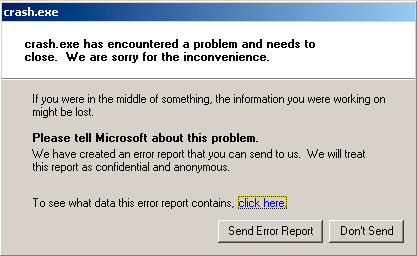
\includegraphics[scale=0.66]{OS-specific/SEH/1/crash_xp1.png}
\caption{Windows XP}
\end{figure}

\begin{figure}[H]
\centering
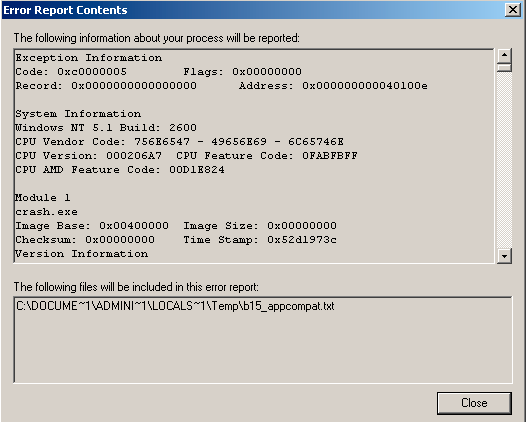
\includegraphics[scale=0.66]{OS-specific/SEH/1/crash_xp2.png}
\caption{Windows XP}
\end{figure}

\begin{figure}[H]
\centering
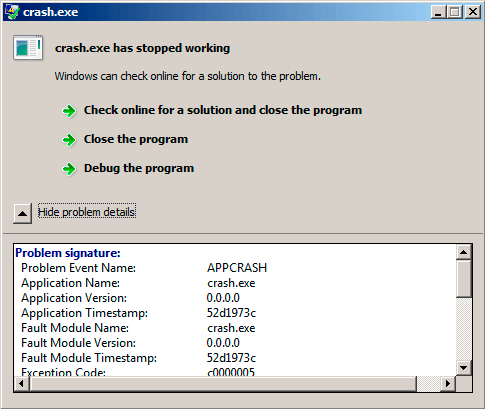
\includegraphics[scale=0.66]{OS-specific/SEH/1/crash_win7.png}
\caption{Windows 7}
\end{figure}

\begin{figure}[H]
\centering
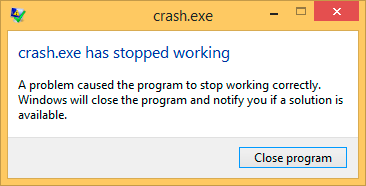
\includegraphics[scale=0.66]{OS-specific/SEH/1/crash_win81.png}
\caption{Windows 8.1}
\end{figure}

\IFRU{Раньше этот обработчик назывался Dr. Watson}{This handler was also called Dr. Watson earlier}
\footnote{\url{https://en.wikipedia.org/wiki/Dr._Watson_(debugger)}}.

\IFRU{Кстати, некоторые разработчики делают свой собственный обработчик,
отправляющий информацию о падении программы им самим}
{By the way, some developers made their own handler, sending information about program crash to themselves}.
\index{Win32!SetUnhandledExceptionFilter()}
\IFRU{Он регистрируется при помощи ф-ции}{It is registered with the help of} \TT{SetUnhandledExceptionFilter()} 
\IFRU{и будет вызван если \ac{OS} не знает как иначе обработать исключение}{and will be called if
\ac{OS} do not have any other way to handle exception}.
\index{Oracle RDBMS}
\IFRU{А, например,}{Other example is} Oracle RDBMS \IFRU{в этом случае генерирует огромные дампы, 
содержащие всю возможную информацию и состоянии \ac{CPU} и памяти}
{it saves huge dumps containing all possible information about \ac{CPU} and memory state}.

\IFRU{Попробуем написать свой примитивный обработчик исключений}
{Let's write our own primitive exception handler}
\footnote{
	\IFRU{Пример основан на примере из}{The example is based on the example from} \cite{PietrekSEH}

	\IFRU{Он должен компилироваться с опцией}{It is compiled with the} SAFESEH\IFRU{}{ option}: 
	\TT{cl seh1.cpp /link /safeseh:no}

	\href{http://msdn.microsoft.com/en-us/library/9a89h429.aspx}
	{\IFRU{Подробнее об опции}{More about} SAFESEH}
}:

\lstinputlisting{OS-specific/SEH/1/1.cpp}

\IFRU{Сегментный регистр FS: в win32 указывает на \ac{TIB}}
{FS: segment register is pointing to the \ac{TIB} in win32}.
\IFRU{Самый первый элемент \ac{TIB} это указатель на последний обработчик в цепочке}
{The very first element in \ac{TIB} is a pointer to the last handler in chain}.
\IFRU{Мы сохраняем его в стеке и записываем туда адрес своего обработчика}{We saving it in the stack and store
an address of our handler there}.
\IFRU{Эта структура называется}{The structure is named} \TT{\_EXCEPTION\_REGISTRATION}, 
\IFRU{это простейший односвязный список, и эти элементы хранятся прямо в стеке}{it is a simplest singly-linked
list and its elements are stored right in the stack}.

\begin{lstlisting}[caption=MSVC/VC/crt/src/exsup.inc]
\_EXCEPTION\_REGISTRATION struc
     prev    dd      ?
     handler dd      ?
\_EXCEPTION\_REGISTRATION ends
\end{lstlisting}

\IFRU{Так что каждое поле}{So each} ``handler'' \IFRU{указывает на обработчик,
а каждое поле}{field points to handler and an each} ``prev'' \IFRU{указывает на предыдущую структуру
в стеке}{field points to previous record in the stack}.
\IFRU{Самая последняя структура имеет}{The last record has} \TT{0xFFFFFFFF} (-1) \IFRU{в поле}{in} 
``prev''\IFRU{}{ field}.

\input{OS-specific/SEH/1/tikz}

\IFRU{После инсталляции своего обработчика, вызываем}{When our handler is installed, let's call}
\TT{RaiseException()}
\footnote{\url{http://msdn.microsoft.com/en-us/library/windows/desktop/ms680552(v=vs.85).aspx}}.
\IFRU{Это пользовательские исключения}{This is user exception}. \IFRU{Обработчик проверяет код}{Handler will check
the code}.
\IFRU{Если код}{If the code is} \TT{0xE1223344}, \IFRU{то он возвращает}{it will return} 
\TT{ExceptionContinueExecution},
\IFRU{что сигнализирует системе что обработчик изменил состояние CPU (обычно это EIP/ESP) и что OS может
возобновить исполнение треда}
{which means that handler fixes CPU state (it is usually EIP/ESP) and the OS can resume thread execution}.
\IFRU{Если вы немного измените код так что обработчик будет возвращать}{If to alter the code slightly
so the handler will return} \TT{ExceptionContinueSearch},
\IFRU{то \ac{OS} будет вызывать остальные
обработчики в цепочке, и врядли найдется тот кто обработает ваше исключение,
ведь информации о нем (вернее, его коде) ни у кого нет}
{then \ac{OS} will call other handlers, and very unlikely the one who can handle it will be founded, since
no one have information about it (rather about its code)}.
\IFRU{Вы увидите стандартное окно Windows о падении процесса}{You will see the standard Windows dialog about
process crash}.

\IFRU{Какова разница между системными исключениями и пользовательскими}{What is the difference between
system exceptions and user}? \IFRU{Вот системные}{Here is a system ones}:

\begin{center}
\begin{tabular}{ | l | l | l | }
\hline
\cellcolor{blue!25} \IFRU{как определен в}{as defined in} WinBase.h & 
\cellcolor{blue!25} \IFRU{как определен в}{as defined in} ntstatus.h & 
\cellcolor{blue!25} \IFRU{численное значение}{numerical value} \\
\hline
EXCEPTION\_ACCESS\_VIOLATION          & STATUS\_ACCESS\_VIOLATION           & 0xC0000005 \\
\hline
EXCEPTION\_DATATYPE\_MISALIGNMENT     & STATUS\_DATATYPE\_MISALIGNMENT      & 0x80000002 \\
\hline
EXCEPTION\_BREAKPOINT                & STATUS\_BREAKPOINT                 & 0x80000003 \\
\hline
EXCEPTION\_SINGLE\_STEP               & STATUS\_SINGLE\_STEP                & 0x80000004 \\
\hline
EXCEPTION\_ARRAY\_BOUNDS\_EXCEEDED     & STATUS\_ARRAY\_BOUNDS\_EXCEEDED      & 0xC000008C \\
\hline
EXCEPTION\_FLT\_DENORMAL\_OPERAND      & STATUS\_FLOAT\_DENORMAL\_OPERAND     & 0xC000008D \\
\hline
EXCEPTION\_FLT\_DIVIDE\_BY\_ZERO        & STATUS\_FLOAT\_DIVIDE\_BY\_ZERO       & 0xC000008E \\
\hline
EXCEPTION\_FLT\_INEXACT\_RESULT        & STATUS\_FLOAT\_INEXACT\_RESULT       & 0xC000008F \\
\hline
EXCEPTION\_FLT\_INVALID\_OPERATION     & STATUS\_FLOAT\_INVALID\_OPERATION    & 0xC0000090 \\
\hline
EXCEPTION\_FLT\_OVERFLOW              & STATUS\_FLOAT\_OVERFLOW             & 0xC0000091 \\
\hline
EXCEPTION\_FLT\_STACK\_CHECK           & STATUS\_FLOAT\_STACK\_CHECK          & 0xC0000092 \\
\hline
EXCEPTION\_FLT\_UNDERFLOW             & STATUS\_FLOAT\_UNDERFLOW            & 0xC0000093 \\
\hline
EXCEPTION\_INT\_DIVIDE\_BY\_ZERO        & STATUS\_INTEGER\_DIVIDE\_BY\_ZERO     & 0xC0000094 \\
\hline
EXCEPTION\_INT\_OVERFLOW              & STATUS\_INTEGER\_OVERFLOW           & 0xC0000095 \\
\hline
EXCEPTION\_PRIV\_INSTRUCTION          & STATUS\_PRIVILEGED\_INSTRUCTION     & 0xC0000096 \\
\hline
EXCEPTION\_IN\_PAGE\_ERROR             & STATUS\_IN\_PAGE\_ERROR              & 0xC0000006 \\
\hline
EXCEPTION\_ILLEGAL\_INSTRUCTION       & STATUS\_ILLEGAL\_INSTRUCTION        & 0xC000001D \\
\hline
EXCEPTION\_NONCONTINUABLE\_EXCEPTION  & STATUS\_NONCONTINUABLE\_EXCEPTION   & 0xC0000025 \\
\hline
EXCEPTION\_STACK\_OVERFLOW            & STATUS\_STACK\_OVERFLOW             & 0xC00000FD \\
\hline
EXCEPTION\_INVALID\_DISPOSITION       & STATUS\_INVALID\_DISPOSITION        & 0xC0000026 \\
\hline
EXCEPTION\_GUARD\_PAGE                & STATUS\_GUARD\_PAGE\_VIOLATION       & 0x80000001 \\
\hline
EXCEPTION\_INVALID\_HANDLE            & STATUS\_INVALID\_HANDLE             & 0xC0000008 \\
\hline
EXCEPTION\_POSSIBLE\_DEADLOCK         & STATUS\_POSSIBLE\_DEADLOCK          & 0xC0000194 \\
\hline
CONTROL\_C\_EXIT                      & STATUS\_CONTROL\_C\_EXIT             & 0xC000013A \\
\hline
\end{tabular}
\end{center}

\IFRU{Так определяется код}{That is how code is defined}:

\begin{center}
\begin{bytefield}{32}
\bitheader[endianness=big]{31,29,28,27,16,15,0} \\
\bitbox{2}{\TT{S}} & 
\bitbox{1}{\TT{U}} &
\bitbox{1}{0} & 
\bitbox{12}{Facility code} &
\bitbox{16}{Error code}
\end{bytefield}
\end{center}

S \IFRU{это код статуса}{is a basic status code}: 
11\EMDASH{}\IFRU{ошибка}{error};
10\EMDASH{}\IFRU{предупреждение}{warning};
01\EMDASH{}\IFRU{информация}{informational};
00\EMDASH{}\IFRU{успех}{success}.
U\EMDASH\IFRU{является ли этот код пользовательским а не системным}{whether the code is user code}.

\IFRU{Вот почему я выбрал}{That is why I chose} 0xE1223344\EMDASH{}
%E\textsubscript{16} (1110\textsubscript{2}) 
0xE (1110b) 
\IFRU{означает что это 1) пользовательское исключение; 2) ошибка}{mean this is 1) user exception; 2) error}.
\IFRU{Хотя, если быть честным, этот пример нормально работает и без этих старших бит}
{But to be honest, this example works finely without these high bits}.

\IFRU{Далее мы пытаемся прочитать значение из памяти по адресу 0}{Then we try to read a value from memory
at the 0th address}.
\IFRU{Конечно, в win32 по этому адресу обычно ничего нет, и сработает исключение}
{Of course, there are nothing at this address in win32, so exception is raised}.
\IFRU{Однако, первый обработчик, который будет заниматься этим делом ~--- ваш, и он узнает об этом
первым, проверяя код на соответствие с константной \TT{EXCEPTION\_ACCESS\_VIOLATION}}
{However, the very first handler will be called --- yours, it will be notified first, checking
the code on equality to the \TT{EXCEPTION\_ACCESS\_VIOLATION} constant}.

\IFRU{А если заглянуть в то что получилось на ассемблере,
то можно увидеть что код читающий из памяти по адресу 0, выглядит так}{The code reading from memory at
0th address is looks like}:

\lstinputlisting[caption=MSVC 2010]{OS-specific/SEH/1/1_fragment.asm}

\IFRU{Возможно ли ``на лету'' исправить ошибку и предложить программе исполняться далее}
{Will it be possible to fix error ``on fly'' and to continue program execution}?
\IFRU{Да, наш обработчик может изменить значение в \EAX и предложить \ac{OS} исполнить эту же инструкцию еще раз}
{Yes, our exception handler can fix \EAX value and now let \ac{OS} will execute this instruction once again}.
\IFRU{Что мы и делаем}{So that is what we do}. \printf \IFRU{напечатает}{will print} 1234,
\IFRU{потому что после работы нашего обработчика}{because, after execution of our handler},
\EAX \IFRU{будет не}{will not be} 0,
\IFRU{а будет содержать адрес глобальной переменной}{it will contain address of global variable} \TT{new\_value}.
\IFRU{Программа будет исполняться далее}{Execution will be resumed}.

\IFRU{Собственно, вот что происходит}{That is what is going on}: 
\IFRU{срабатывает защита менеджера памяти в \ac{CPU}}{memory manager in \ac{CPU} signalling about error}, 
\IFRU{он останавливает работу треда}{the \ac{CPU} suspends the thread},
\IFRU{отыскивает в ядре Windows обработчик исключений}{it finds exception handler in the Windows kernel}, 
\IFRU{тот, в свою очередь, начинает вызывать обработчики из цепочки \ac{SEH}, по одному}
{latter, in turn, is starting to call all handlers in \ac{SEH} chain, one by one}.

\IFRU{Я компилирую это всё в MSVC 2010, но конечно же, нет никакой гарантии 
что для указателя будет использован именно регистр \EAX}{I use MSVC 2010 now, but of course,
there are no any guarantee that \EAX will be used for pointer}.

\IFRU{Этот трюк с подменой адреса эффектно выглядит, 
и я его привожу здесь для наглядной иллюстрации работы \ac{SEH}}
{This address replacement trick is looks showingly, and I offer it here for \ac{SEH} internals illustration}.
\IFRU{Тем не менее, я затрудняюсь
припомнить, применяется ли где-то подобное на практике для исправления ошибок ``на лету''}
{Nevertheless, I cannot recall
where it is used for ``on-fly'' error fixing in practice}.

\IFRU{Почему SEH-записи хранятся именно в стеке а не в каком-то другом месте}
{Why SEH-related records are stored right in the stack instead of some other place}?
\IFRU{Вероятно, потому что тогда \ac{OS} не будет заботиться об освобождении этой информации, эти записи
пропадают как ненужные когда ф-ция заканчивает работу}
{Supposedly because then \ac{OS} will not need to care about freeing this information, these records
will be disposed when function finishing its execution}.
\IFRU{Но я не уверен на}{But I'm not} 100\%\IFRU{ и могу ошибаться}{-sure and can be wrong}.
\IFRU{Это чем-то похоже на}{This is somewhat like} alloca(): (\ref{alloca}).


\subsection{\IFRU{Теперь вспомним MSVC}{Now let's get back to MSVC}}

\index{\Cpp!\IFRU{исключения}{exceptions}}
\IFRU{Должно быть, программистам Microsoft были нужны исключения в Си, но не в Си++, так что они добавили
нестандартное расширение Си в MSVC}
{Supposedly, Microsoft programmers need exceptions in C, but not in C++, so they added a non-standard C extension
to MSVC}\footnote{\url{http://msdn.microsoft.com/en-us/library/swezty51.aspx}}.
\IFRU{Оно не связано с исключениями в Си++}{It is not related to C++ \ac{PL} exceptions}.

\begin{lstlisting}
__try
{
    ...
}
__except(filter code)
{
    handler code
}
\end{lstlisting}

\IFRU{Блок ``finally'' может присутствовать вместо код обработчика}{``Finally'' block may be instead of handler code}:

\begin{lstlisting}
__try
{
    ...
}
__finally
{
    ...
}
\end{lstlisting}

\IFRU{Код-фильтр это выражение, отвечающее на вопрос, соответствует ли код этого обработчика к поднятому исключению}
{The filter code is an expression, telling whether this handler code is coressponding to the exception raised}.
\IFRU{Если ваш код слишком большой и не помещается в одно выражение, отдельная функция-фильтр может быть определена}
{If your code is too big and cannot be fitted into one expression, a separate filter function can be defined}.

\IFRU{Таких конструкций много в ядре Windows}{There are a lot of such constructs in the Windows kernel}.

\IFRU{Вот несколько примеров оттуда}{Here is couple of examples from there} (\ac{WRK}):

\lstinputlisting[caption=WRK-v1.2/base/ntos/ob/obwait.c]{OS-specific/SEH/2/wrk_ex1.c}

\lstinputlisting[caption=WRK-v1.2/base/ntos/cache/cachesub.c]{OS-specific/SEH/2/wrk_ex2.c}

\IFRU{Вот пример кода-фильтра}{Here is also filter code example}:

\lstinputlisting[caption=WRK-v1.2/base/ntos/cache/copysup.c]{OS-specific/SEH/2/wrk_ex3.c}

\IFRU{Внутри, SEH это расширение исключений поддерживаемых OS}{Internally, SEH is an extension of OS-supported exceptions}.
\IFRU{Но функция обработчик теперь или}{But the handler function is} \TT{\_except\_handler3} (\ForENRU SEH3) 
\OrENRU \TT{\_except\_handler4} (\ForENRU SEH4).
\IFRU{Код обработчика от MSVC, расположен в его библиотеках, или же в}
{The code of this handler is MSVC-related, it is located in its libraries, or in} msvcr*.dll.
\IFRU{Очень важно понимать что SEH это специфичное для MSVC}{It is very important to know that SEH is MSVC-specific thing}.
\IFRU{Другие компиляторы могут предлагать что-то совершенно другое}
{Other compilers may offer something completely different}.

\subsubsection{SEH3}

SEH3 \IFRU{имеет}{has} \TT{\_except\_handler3} \IFRU{как функцию-обработчик, и расширяет структуру}
{as handler functions, and extends} \TT{\_EXCEPTION\_REGISTRATION} \IFRU{добавляя указатель на \IT{scope table}
и переменную \IT{previous try level}}{table, adding
a pointer to the \IT{scope table} and \IT{previous try level} variable}.
SEH4 \IFRU{расширяет}{extends} \IT{scope table} \IFRU{добавляя еще 4 значения связанных с защитой от переполнения буфера}
{by 4 values for buffer overflow protection}.

\IT{Scope table} \IFRU{это таблица, состоящая из указателей на код фильтра и обработчика, для каждого уровня вложенности
\IT{try/except}}{is a table consisting of pointers to the filter and handler codes, for each level of \IT{try/except}
nestedness}.

\input{OS-specific/SEH/2/tikz}

\IFRU{И снова, очень важно понимать, что OS заботится только о полях}
{Again, it is very important to understand that OS take care only of} \IT{prev/handle}
\IFRU{, и больше ничего}{ fields, and nothing more}.
\IFRU{Это работа функции}{It is job of} \TT{\_except\_handler3} \IFRU{читать другие поля, читать \IT{scope table}
и решать, какой обработчик исполнять и когда}{function to read other fields, read \IT{scope table}, and decide,
which handler to execute and when}.

\index{Wine}
\index{ReactOS}
\IFRU{Исходный код ф-ции}{The source code of} \TT{\_except\_handler3} \IFRU{закрыт}{function is closed}.
\IFRU{Хотя, Sanos OS, имеющая слой совместимости с win32, имеет некоторые ф-ции написанные заново, которые
в каком-то смысле эквивалентны тем что в Windows}
{However, Sanos OS, which have win32 compatibility layer, has the same
functions redeveloped, which are somewhat equivalent to those in Windows}
\footnote{\url{https://code.google.com/p/sanos/source/browse/src/win32/msvcrt/except.c}}.
\IFRU{Другие попытки реализации имеются в}{Another reimplementations are present in} 
Wine\footnote{\url{https://github.com/mirrors/wine/blob/master/dlls/msvcrt/except_i386.c}}
\AndENRU 
ReactOS\footnote{\url{http://doxygen.reactos.org/d4/df2/lib_2sdk_2crt_2except_2except_8c_source.html}}.

\IFRU{Если указатель}{If the} \IT{filter} \IFRU{ноль}{pointer is zero}, \IT{handler} \IFRU{указывает на код \IT{finally}}
{pointer is the pointer to a \IT{finally} code}.

\IFRU{Во время исполнения, значение}{During execution,} \IT{previous try level} \IFRU{в стеке меняется,
чтобы ф-ция}{value in the stack is changing, so the} \TT{\_except\_handler3} \IFRU{знала о текущем уровне вложенности,
чтобы знать, какой элемент таблицы}{will know about current
state of nestedness, in order to know which} \IT{scope table} \IFRU{использовать}{entry to use}.

\subsubsection{SEH3: \IFRU{пример с одним блоком try/except}{one try/except block example}}

\lstinputlisting{OS-specific/SEH/2/2.c}

\lstinputlisting[caption=MSVC 2003]{OS-specific/SEH/2/2_SEH3.asm}

\IFRU{Здесь мы видим как структура SEH конструируется в стеке}{Here we see how SEH frame is being constructed in the stack}.
\IT{Scope table} \IFRU{расположена в сегменте}{is located in the} \TT{CONST}\IFRU{}{ segment}\EMDASH{}
\IFRU{действительно, эти поля не будут меняться}{indeed, these fields will not be changed}.
\IFRU{Интересно, как меняется переменная}{An interesting thing is how} \IT{previous try level}\IFRU{}{ variable is changed}.
\IFRU{Исходное значение}{Initial value is} \TT{0xffffffff} ($-1$).
\IFRU{Момент, когда тело}{The moment when body of} \TT{try} \IFRU{открывается, обозначен инструкцией, записывающей}
{statement is opened is marked as an instruction writing} $0$ \IFRU{в эту переменную}{to the variable}.
\IFRU{В момент, когда тело}{The moment when body of} \TT{try} \IFRU{закрывается}{statement is closed}, $-1$ 
\IFRU{возвращается в нее назад}{is returned back to it}.
\IFRU{Мы так же видим адреса кода фильтра и обработчика}{We also see addresses of filter and handler code}.
\IFRU{Так мы можем легко увидеть структуру конструкций \IT{try/except} в ф-ции}
{Thus we can easily see the structure of \IT{try/except} constructs in the function}.

\IFRU{Так как код инициализации SEH-структур в прологе ф-ций может быть общим для нескольких ф-ций, иногда компилятор
вставляет в прологе вызов ф-ции}{Since the SEH setup code in the function prologue may be shared between many of functions,
sometimes compiler inserts a call to} \TT{SEH\_prolog()}\IFRU{, которая всё это делает}
{ function in the prologue, which do that}.

\IFRU{Запустим этот пример в}{Let's try to run this example in} \tracer{}:

\begin{lstlisting}
tracer.exe -l:2.exe --dump-seh
\end{lstlisting}

\begin{lstlisting}[caption=tracer.exe output]
EXCEPTION_ACCESS_VIOLATION at 2.exe!main+0x44 (0x401054) ExceptionInformation[0]=1
EAX=0x00000000 EBX=0x7efde000 ECX=0x0040cbc8 EDX=0x0008e3c8
ESI=0x00001db1 EDI=0x00000000 EBP=0x0018feac ESP=0x0018fe80
EIP=0x00401054
FLAGS=AF IF RF
* SEH frame at 0x18fe9c prev=0x18ff78 handler=0x401204 (2.exe!_except_handler3)
SEH3 frame. previous trylevel=0
scopetable entry[0]. previous try level=-1, filter=0x401070 (2.exe!main+0x60) handler=0x401088 (2.exe!main+0x78)
* SEH frame at 0x18ff78 prev=0x18ffc4 handler=0x401204 (2.exe!_except_handler3)
SEH3 frame. previous trylevel=0
scopetable entry[0]. previous try level=-1, filter=0x401531 (2.exe!mainCRTStartup+0x18d) handler=0x401545 (2.exe!mainCRTStartup+0x1a1)
* SEH frame at 0x18ffc4 prev=0x18ffe4 handler=0x771f71f5 (ntdll.dll!__except_handler4)
SEH4 frame. previous trylevel=0
SEH4 header:	GSCookieOffset=0xfffffffe GSCookieXOROffset=0x0
		EHCookieOffset=0xffffffcc EHCookieXOROffset=0x0
scopetable entry[0]. previous try level=-2, filter=0x771f74d0 (ntdll.dll!___safe_se_handler_table+0x20) handler=0x771f90eb (ntdll.dll!_TppTerminateProcess@4+0x43)
* SEH frame at 0x18ffe4 prev=0xffffffff handler=0x77247428 (ntdll.dll!_FinalExceptionHandler@16)
\end{lstlisting}

\IFRU{Мы видим что цепочка SEH состоит из 4-х обработчиков}{We that SEH chain consisting of 4 handlers}. 

\index{CRT}
\IFRU{Первые два расположены в нашем примере}{First two are located in out example}. \IFRU{Два}{Two}?
\IFRU{Но ведь мы же сделали только один}{But we made only one}?
\IFRU{Да, второй был установлен в \ac{CRT}-функции}{Yes, another one is setting up in \ac{CRT} function} 
\TT{\_mainCRTStartup()}, \IFRU{и судя по всему, он обрабатывает как минимум исключения связанные с \ac{FPU}}
{and as it seems, it handles at least \ac{FPU} exceptions}.
\IFRU{Его код можно посмотреть в инсталляции MSVC}{Its source code can found in MSVS installation}: \TT{crt/src/winxfltr.c}.

\IFRU{Третий это SEH4 в}{Third is SEH4 frame in} ntdll.dll, \IFRU{и четвертый это обработчик, не имеющий отношения к MSVC,
расположенный в}
{and the fourth handler is not MSVC-related located in} ntdll.dll,
\IFRU{имеющий ``говорящее'' название ф-ции}{and it has self-describing function name}.

\IFRU{Как видно, в цепочке присутствуют обработчики трех типов}{As you can see, there are 3 types of handlers in one chain}:
\IFRU{один не связан с MSVC вообще (последний) и два связанных с MSVC}
{one is not related to MSVC at all (the last one) and two MSVC-related}: SEH3 \AndENRU SEH4.

\subsubsection{SEH3: \IFRU{пример с двумя блоками try/except}{two try/except blocks example}}

\lstinputlisting{OS-specific/SEH/2/3.c}

\IFRU{Теперь здесь два блока \TT{try}}{Now there are two \TT{try} blocks}.
\IFRU{Так что}{So the} \IT{scope table} \IFRU{теперь содержит два элемента, один элемент на каждый блок}
{now have two entries, each entry for each block}.
\IT{Previous try level} \IFRU{меняется вместе с тем, как исполнение доходит до очередного \TT{try}-блока, либо
выходит из него}{is changing as execution flow entering or exiting \TT{try} block}.

\lstinputlisting[caption=MSVC 2003]{OS-specific/SEH/2/3_SEH3.asm}

\IFRU{Если установить брякпоинт на ф-цию}{If to set a breakpoint on} \printf{} \IFRU{вызываемую из обработчика,
мы можем увидеть что добавился еще один SEH-обработчик}{function which is called from the handler, 
we may also see how yet another SEH handler is added}.
\IFRU{Наверное, это еще какая-то дополнительная механика скрытая внутри процесса обработки исключений}
{Perhaps, yet another machinery inside of SEH handling process}.
\IFRU{Тут мы также видим}{Here we also see our} \IT{scope table} \IFRU{состояющую из двух элементов}
{consisting of 2 entries}.

\begin{lstlisting}
tracer.exe -l:3.exe bpx=3.exe!printf --dump-seh
\end{lstlisting}

\begin{lstlisting}[caption=tracer.exe output]
(0) 3.exe!printf
EAX=0x0000001b EBX=0x00000000 ECX=0x0040cc58 EDX=0x0008e3c8
ESI=0x00000000 EDI=0x00000000 EBP=0x0018f840 ESP=0x0018f838
EIP=0x004011b6
FLAGS=PF ZF IF
* SEH frame at 0x18f88c prev=0x18fe9c handler=0x771db4ad (ntdll.dll!ExecuteHandler2@20+0x3a)
* SEH frame at 0x18fe9c prev=0x18ff78 handler=0x4012e0 (3.exe!_except_handler3)
SEH3 frame. previous trylevel=1
scopetable entry[0]. previous try level=-1, filter=0x401120 (3.exe!main+0xb0) handler=0x40113b (3.exe!main+0xcb)
scopetable entry[1]. previous try level=0, filter=0x4010e8 (3.exe!main+0x78) handler=0x401100 (3.exe!main+0x90)
* SEH frame at 0x18ff78 prev=0x18ffc4 handler=0x4012e0 (3.exe!_except_handler3)
SEH3 frame. previous trylevel=0
scopetable entry[0]. previous try level=-1, filter=0x40160d (3.exe!mainCRTStartup+0x18d) handler=0x401621 (3.exe!mainCRTStartup+0x1a1)
* SEH frame at 0x18ffc4 prev=0x18ffe4 handler=0x771f71f5 (ntdll.dll!__except_handler4)
SEH4 frame. previous trylevel=0
SEH4 header:	GSCookieOffset=0xfffffffe GSCookieXOROffset=0x0
		EHCookieOffset=0xffffffcc EHCookieXOROffset=0x0
scopetable entry[0]. previous try level=-2, filter=0x771f74d0 (ntdll.dll!___safe_se_handler_table+0x20) handler=0x771f90eb (ntdll.dll!_TppTerminateProcess@4+0x43)
* SEH frame at 0x18ffe4 prev=0xffffffff handler=0x77247428 (ntdll.dll!_FinalExceptionHandler@16)
\end{lstlisting}

\subsubsection{SEH4}

\index{\BufferOverflow}
\index{Security cookie}
\IFRU{Во время атаки переполнения буфера}{During buffer overflow} (\ref{subsec:bufferoverflow})
\IFRU{адрес}{attack, address of the} \IT{scope table} \IFRU{может быть перезаписан, так что начиная с}
{can be rewritten, so starting at} MSVC 2005, SEH3 \IFRU{был дополнен защитой от переполнения буфера, до SEH4}
{was upgraded to SEH4 in order to have buffer overflow protection}.
\IFRU{Указатель на}{The pointer to} \IT{scope table} \IFRU{теперь}{is now} \glslink{xoring}{\IFRU{про-XOR-ен}{xored}} 
\IFRU{с}{with} \gls{security cookie}.
\IT{Scope table} \IFRU{расширена, теперь имеет заголовок содержающий 2 указателя на}
{extended to have a header, consisting of two pointers to} \IT{security cookies}.
\IFRU{Каждый элемент имеет смешение внутри стека на другое значение: это адрес фрейма (EBP) также}
{Each element have an offset inside of stack of another value: 
this is address of stack frame (EBP)} \glslink{xoring}{\IFRU{про-XOR-еный}{xored}} \IFRU{с}{with} 
\TT{security\_cookie} \IFRU{расположенный в стеке}{as well, placed in the stack}.
\IFRU{Это значение будет прочитано во время обработки исключения и проверено на правильность}
{This value will be read during exception handling and checked, if it is correct}.
\IT{Security cookie} \IFRU{в стеке случайное каждый раз, так что атакующий, как мы надеемся, не мог предсказать его}
{in the stack is random each time, so remote attacker, hopefully, will not be able to predict it}.

\IFRU{Изначальное значение}{Initial} \IT{previous try level} \IFRU{это}{is} $-2$ \InENRU SEH4 \IFRU{вместо}{instead of} $-1$.

\def\SEHfour{1}
\input{OS-specific/SEH/2/tikz}

\IFRU{Оба примера скомпилированные в}{Here is both examples compiled in} MSVC 2012 \IFRU{с}{with} SEH4:

\lstinputlisting[caption=MSVC 2012: one try block example]{OS-specific/SEH/2/2_SEH4.asm}

\lstinputlisting[caption=MSVC 2012: two try blocks example]{OS-specific/SEH/2/3_SEH4.asm}

\IFRU{Вот значение}{Here is a meaning of} \IT{cookies}: \TT{Cookie Offset} 
\IFRU{это разница между адресом записанного в стеке значения EBP и значения}
{is a difference between address of saved EBP value in stack
and the} $EBP \oplus security\_cookie$ \IFRU{в стеке}{value in the stack}.
\TT{Cookie XOR Offset} \IFRU{это дополнительная разница между значением}{is additional difference between} 
$EBP \oplus security\_cookie$ \IFRU{и тем что записано в стеке}{value and what is
stored in the stack}.
\IFRU{Если это уравнение не верно, то процесс остановится из-за разрушения стека}
{If this equation is not true, a process will be stopped due to stack corruption}:

\begin{center}
$security\_cookie \oplus (CookieXOROffset + address of saved EBP) == stack[address of saved EBP + CookieOffset]$
\end{center}

\IFRU{Если}{If} \TT{Cookie Offset} \IFRU{равно}{is} $-2$, \IFRU{это значит что оно не присутствует}{it is not present}.

\IFRU{Проверка \IT{cookies} также реализована в моем}{\IT{Cookies} checking is also implemented in my} \tracer{},
\IFRU{смотрите}{see} \url{https://github.com/dennis714/tracer/blob/master/SEH.c} \IFRU{для деталей}{for details}. 

\IFRU{Возможность переключиться назад на SEH3 все еще присутствует в компиляторах после (и включая) MSVC 2005, нужно включить
опцию \TT{/GS-}, впрочем, \ac{CRT}-код будет продолжать использовать SEH4}
{It is still possible to fall back to SEH3 in the compilers after (and including) MSVC 2005 by setting \TT{/GS-} option,
however, \ac{CRT} code will use SEH4 anyway}.



\subsection{\IFRU{Больше о}{Read more about} SEH}

\cite{PietrekSEH}, \cite{IgorSkochinsky}.


\part{\RU{Инструменты}\EN{Tools}}

\chapter{\RU{Дизассемблер}\EN{Disassembler}}

\section{IDA}

\label{IDA}
\RU{Старая бесплатная версия доступна для скачивания}\EN{Older freeware version is available for downloading}
\footnote{\url{http://www.hex-rays.com/idapro/idadownfreeware.htm}}.

\ShortHotKeyCheatsheet: \ref{sec:IDA_cheatsheet}

\chapter{\RU{Отладчик}\EN{Debugger}}

\section{tracer}

\index{tracer}
\label{tracer}
\RU{Я использую}\EN{I use} \IT{tracer}\footnote{\url{http://yurichev.com/tracer-\LANG.html}}
\RU{вместо отладчика}\EN{instead of debugger}.

\RU{Со временем я отказался использовать отладчик, потому что все что мне нужно от него: это иногда подсмотреть 
какие-либо аргументы какой-либо функции во время исполнения или состояние регистров в определенном месте. 
Каждый раз загружать отладчик для этого это слишком, поэтому я написал очень простую утилиту \IT{tracer}. 
Она консольная, запускается из командной строки, позволяет перехватывать исполнение функций, 
ставить брякпойнты на произвольные места, смотреть состояние регистров, модифицировать их, и так далее.}
\EN{I stopped to use debugger eventually, since all I need from it is to spot a function's arguments while
execution, or registers' state at some point.
To load debugger each time is too much, so I wrote a small utility \IT{tracer}.
It has console-interface, working from command-line, enable us to intercept function execution,
set breakpoints at arbitrary places, spot registers' state, modify it, etc.}

\RU{Но для учебы, очень полезно трассировать код руками в отладчике, наблюдать как меняются значения регистров 
(например, как минимум классический SoftICE, OllyDbg, WinDbg подсвечивают измененные регистры), 
флагов, данные, менять их самому, смотреть реакцию, и т.д.}
\EN{However, as for learning purposes, it is highly advisable to trace code in debugger manually, watch how register's state
changing (e.g. classic SoftICE, OllyDbg, WinDbg highlighting changed registers), flags, data, change them
manually, watch reaction, etc.}

\section{\olly}
\index{\olly}

\RU{Очень популярный отладчик пользовательской среды win32}\EN{Very popular user-mode win32 debugger}:\\
\url{http://www.ollydbg.de/}.

\ShortHotKeyCheatsheet: \label{sec:Olly_cheatsheet}

\section{GDB}
\index{GDB}

\RU{Не очень популярный отладчик у реверсеров, тем не менее, крайне удобный}\EN{Not very popular
debugger among reverse engineers, but very comfortable nevertheless}.
\RU{Некоторые команды}\EN{Some commands}: \ref{sec:GDB_cheatsheet}.

\chapter{\RU{Трассировка системных вызовов}\EN{System calls tracing}}

\label{strace}
\index{strace}
\index{dtruss}
\subsection{strace / dtruss}

\index{syscalls}
\RU{Позволяет показать, какие системные вызовы (syscalls(\ref{syscalls})) прямо сейчас вызывает процесс}
\EN{Will show which system calls (syscalls(\ref{syscalls})) are called by process right now}.
\RU{Например}\EN{For example}:

\begin{lstlisting}
# strace df -h

...

access("/etc/ld.so.nohwcap", F_OK)      = -1 ENOENT (No such file or directory)
open("/lib/i386-linux-gnu/libc.so.6", O_RDONLY|O_CLOEXEC) = 3
read(3, "\177ELF\1\1\1\0\0\0\0\0\0\0\0\0\3\0\3\0\1\0\0\0\220\232\1\0004\0\0\0"..., 512) = 512
fstat64(3, {st_mode=S_IFREG|0755, st_size=1770984, ...}) = 0
mmap2(NULL, 1780508, PROT_READ|PROT_EXEC, MAP_PRIVATE|MAP_DENYWRITE, 3, 0) = 0xb75b3000
\end{lstlisting}

\index{\MacOSX}
\RU{В \MacOSX для этого же имеется dtruss}\EN{\MacOSX has dtruss for the same aim}.

\index{cygwin}
\RU{В Cygwin также есть strace, впрочем, если я верно понял, 
он показывает результаты только для .exe-файлов скомпилированных для среды самого cygwin}
\EN{The Cygwin also has strace, but if I understood correctly, it works only for .exe-files
compiled for cygwin environment itself}.

\chapter{\RU{Декомпиляторы}\EN{Decompilers}}

\RU{Пока существует только один, публично доступный, декомпилятор в Си высокого качества}
\EN{There are only one known, publically available, high-quality decompiler to C code}: Hex-Rays:\\
\url{https://www.hex-rays.com/products/decompiler/}

% TODO Java, .NET, VB, etc

\chapter{\RU{Прочие инструменты}\EN{Other tools}}

\begin{itemize}
\item
Microsoft Visual Studio Express\footnote{\url{http://www.microsoft.com/express/Downloads/}}:
\RU{Усеченная бесплатная версия Visual Studio, пригодная для простых экспериментов}
\EN{Stripped-down free Visual Studio version, convenient for simple experiments}.
Some useful options: \ref{sec:MSVC_options}.

\item
\label{Hiew}
Hiew\footnote{\url{http://www.hiew.ru/}} \RU{для мелкой модификации кода в исполняемых файлах}
\EN{for small modifications of code in binary files}.

\item
\index{binary grep}
binary grep: \RU{небольшая утилита для поиска констант (либо просто последовательности байт)
в большом  кол-ве файлов, включая неисполняемые: \BGREPURL.}
\EN{the small utility for constants searching (or just any byte sequence) in a big pile of files, 
including non-executable: \BGREPURL.}
\end{itemize}


\chapter{\RU{Примеры из практики}\EN{Examples from practice}}

%\clearpage
\begin{center}
\vspace*{\fill}

\begin{figure}[H]
\centering
\myincludegraphics{cover4.jpg}
\end{figure}

\vspace*{\fill}
\end{center}

\clearpage

% sections here
\chapter{\EN{Task manager practical joke}\RU{Шутка с task manager} (Windows Vista)}

\RU{У меня только 4 ядра в процессоре в компьютере, так что Task Manager в Windows показывает только 4
графика загрузки процессора.}
\EN{I have only 4 CPU cores on my computer, so the Windows Task Manager shows only 4 CPU load graphs.}

\RU{Посмотрим, сможем ли мы немного хакнуть Task Manager, чтобы он находил больше ядер в компьютере.}
\EN{Let's see if it's possible to hack Task Manager slightly so it would detect more CPU cores on a computer.}

\RU{В начале задумаемся, откуда Task Manager знает количество ядер?}
\EN{Let us first think, how Task Manager would know number of cores?}
\RU{В win32 имеется ф-ция \TT{GetSystemInfo()}, при помощи которой можно узнать.}
\EN{There are \TT{GetSystemInfo()} win32 function present in win32 userspace which can tell us this.}
\RU{Но она не импортируется в}\EN{But it's not imported in} \TT{taskmgr.exe}.
\RU{Есть еще одна в \gls{NTAPI}, \TT{NtQuerySystemInformation()}, которая используется в 
\TT{taskmgr.exe} в ряде мест.}
\EN{There are, however, another one in \gls{NTAPI}, \TT{NtQuerySystemInformation()}, 
which is used in \TT{taskmgr.exe} in several places.}
\RU{Чтобы узнать количество ядер, нужно вызвать эту ф-цию с константной \TT{SystemBasicInformation} в 
первом аргументе (а это ноль}
\EN{To get number of cores, one should call this function with \TT{SystemBasicInformation} constant 
in first argument (which is zero}
\footnote{MSDN: \url{http://msdn.microsoft.com/en-us/library/windows/desktop/ms724509(v=vs.85).aspx}}).

\RU{Второй аргумент должен указывать на буфер, который примет всю информацию.}
\EN{Second argument should point to the buffer, which will receive all the information.}

\RU{Так что нам нужно найти все вызовы ф-ции \TT{NtQuerySystemInformation(0, ?, ?, ?)}.}
\EN{So we need to find all calls to the \TT{NtQuerySystemInformation(0, ?, ?, ?)} function.}
\RU{Откроем}\EN{Let's open} \TT{taskmgr.exe} \InENRU IDA. 
\RU{Что всегда хорошо с исполняемыми файлами от Microsoft, это то что IDA может скачать соответствующуий 
\gls{PDB}-файл именно для этого файла и добавить все имена ф-ций.}
\EN{What is always good about Microsoft executables is that IDA can download corresponding \gls{PDB} 
file for exactly this executable and add all function names.}
\RU{Видимо, Task Manager написан на C++ и некоторые ф-ции и классы имеют говорящие за себя имена.}
\EN{It seems, Task Manager written in C++ and some of function names and classes are really 
speaking for themselves.}
\RU{Тут есть классы}\EN{There are classes} CAdapter, CNetPage, CPerfPage, CProcInfo, CProcPage, CSvcPage, 
CTaskPage, CUserPage.
\RU{Должно быть, каждый класс соответствует каждой вкладке в Task Manager.}
\EN{Apparently, each class corresponding each tab in Task Manager.}

\RU{Я прошелся по всем вызовам и добавил комментарий с числом, передающимся как первый аргумент.}
\EN{I visited each call and I add comment with a value which is passed as the first function argument.}
\RU{В некоторых местах я написал ``not zero'', потому что значение в тех местах однозначно не ноль, 
но что-то другое (больше об этом во второй части главы).}
\EN{There are ``not zero'' I wrote at some places, because, the value there was not clearly zero, 
but something really different (more about this in the second part of this chapter).}
\RU{А мы все-таки ищем ноль передаваемый как аргумент.}
\EN{And we are looking for zero passed as argument after all.}

\begin{figure}[H]
\centering
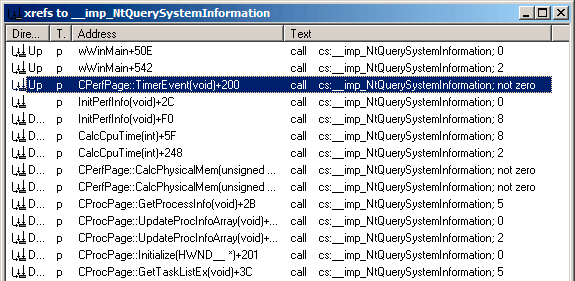
\includegraphics[scale=\FigScale]{examples/taskmgr/IDA_xrefs.png}
\caption{IDA: \RU{вызовы ф-ции}\EN{cross references to} NtQuerySystemInformation()}
\end{figure}

\RU{Да, имена действительно говорящие сами за себя.}
\EN{Yes, the names are really speaking for themselves.}

\RU{Когда я внимательно изучил каждое место, где вызывается \TT{NtQuerySystemInformation(0, ?, ?, ?)},
я быстро нашел то что нужно в ф-ции \TT{InitPerfInfo()}:}
\EN{When I closely investigating each place where \TT{NtQuerySystemInformation(0, ?, ?, ?)} is called,
I quickly found what I need in the \TT{InitPerfInfo()} function:}

\lstinputlisting[caption=taskmgr.exe (Windows Vista)]{examples/taskmgr/taskmgr.lst}

\TT{g\_cProcessors} \RU{это глобальная переменная и это имя присвоено IDA в соответствии с \gls{PDB}-файлом,
скачанным с сервера символов Microsoft}\EN{is a global variable, and this name was assigned by 
IDA according to \gls{PDB} loaded from the Microsoft symbol server}.

\RU{Байт берется из}\EN{The byte is taken from} \TT{var\_C20}. 
\RU{И}\EN{And} \TT{var\_C58} \RU{передается в}\EN{is passed to} \TT{NtQuerySystemInformation()} 
\RU{как указатель на принимающий буфер}\EN{as a pointer to the receiving buffer}.
\RU{Разница между}\EN{The difference between} 0xC20 \AndENRU 0xC58 \RU{это}\EN{is} 0x38 (56).
\RU{Посмотрим на формат структуры, который можно найти в MSDN:}
\EN{Let's take a look at returning structure format, which we can find in MSDN:}

\begin{lstlisting}
typedef struct _SYSTEM_BASIC_INFORMATION {
    BYTE Reserved1[24];
    PVOID Reserved2[4];
    CCHAR NumberOfProcessors;
} SYSTEM_BASIC_INFORMATION;
\end{lstlisting}

\RU{Это система x64, так что каждый PVOID занимает здесь 8 байт.}
\EN{This is x64 system, so each PVOID takes 8 byte here.}
\RU{Так что все \IT{reserved}-поля занимают $24+4*8=56$.}
\EN{So all \IT{reserved} fields in the structure takes $24+4*8=56$.}
\RU{О да, это значит что }\EN{Oh yes, this means, }\TT{var\_C20} \RU{в локальном стеке это именно поле}\EN{is the 
local stack is exactly} \TT{NumberOfProcessors} \RU{структуры}\EN{field of the} 
\TT{SYSTEM\_BASIC\_INFORMATION}\EN{ structure}.

\RU{Проверим, прав ли я}\EN{Let's check if I'm right}.
\RU{Скопируем}\EN{Copy} \TT{taskmgr.exe} \RU{из}\EN{from} \TT{C:\textbackslash{}Windows\textbackslash{}System32} 
\RU{в какую-нибудь другую папку}\EN{to some other folder} 
(\RU{чтобы}\EN{so the} \IT{Windows Resource Protection} \RU{не пыталась восстанавливать измененный}\EN{will not 
try to restore patched} \TT{taskmgr.exe}).

\RU{Откроем его в Hiew и найдем это место:}
\EN{Let's open it in Hiew and find the place:}

\begin{figure}[H]
\centering
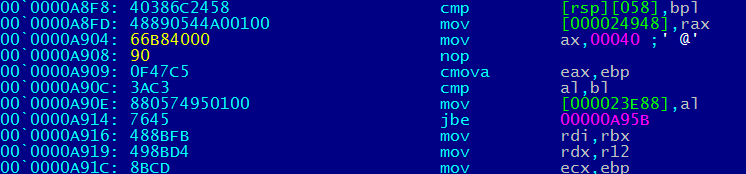
\includegraphics[scale=\FigScale]{examples/taskmgr/hiew1.png}
\caption{Hiew: \RU{найдем это место}\EN{find the place to be patched}}
\end{figure}

\RU{Заменим инструкцию \TT{MOVZX} на нашу.}
\EN{Let's replace \TT{MOVZX} instruction by our.}
\RU{Сделаем вид что у нас 64 ядра процессора}\EN{Let's pretend we've got 64 CPU cores}.
\RU{Добавим дополнительную инструкцию \ac{NOP} (потому что наша инструкция короче чем та что там сейчас):}
\EN{Add one additional \ac{NOP} (because our instruction is shorter than original one):}

\begin{figure}[H]
\centering
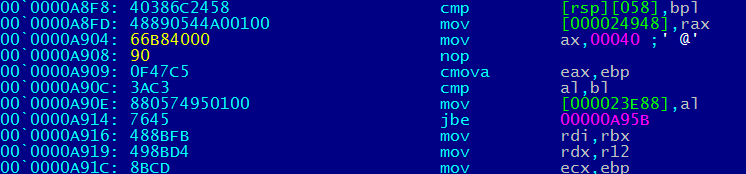
\includegraphics[scale=\FigScale]{examples/taskmgr/hiew1.png}
\caption{Hiew: \RU{меняем инструкцию}\EN{patch it}}
\end{figure}

\RU{И это работает}\EN{And it works}!
\RU{Конечно же, данные в графиках неправильные}\EN{Of course, data in graphs is not correct}.
\RU{Иногда, Task Manager даже показывает общую загрузку CPU более 100\%.}
\EN{At times, Task Manager even shows overall CPU load more than 100\%.}

\begin{figure}[H]
\centering
\includegraphics[scale=\FigScale]{examples/taskmgr/taskmgr_64cpu_crop.png}
\caption{\RU{Обманутый}\EN{Fooled} Windows Task Manager}
\end{figure}

\RU{Я выбрал число 64, потому что Task Manager падает если установить б\'{о}льшее значение.}
\EN{I picked number of 64, because Task Manager is crashing if you try to set larger value.}
\RU{Должно быть, Task Manager в Windows Vista не тестировался на компьютерах с большим количеством ядер.}
\EN{Apparently, Task Manager in Windows Vista was not tested on computer with larger count of cores.}
\RU{И наверное там есть внутри какие-то статичные структуры данных, ограниченные до 64-х ядер.}
\EN{So there are probably some static data structures inside it limited to 64 cores.}

\section{\RU{Использование LEA для загрузки значений}\EN{Using LEA to load values}}

\RU{Иногда, \TT{LEA} используется в \TT{taskmgr.exe} вместо \TT{MOV} для установки первого аргумента 
\TT{NtQuerySystemInformation()}:}
\EN{Sometimes, \TT{LEA} is used in \TT{taskmgr.exe} instead of \TT{MOV} to set first argument of 
\TT{NtQuerySystemInformation()}:}

\lstinputlisting[caption=taskmgr.exe (Windows Vista)]{examples/taskmgr/taskmgr2.lst}

\RU{Честно говоря, я не знаю почему, но \ac{MSVC} часто так делает.}
\EN{I honestly, don't know why, but that is what \ac{MSVC} often does.}
\RU{Может быть, это какая-то оптимизация и \TT{LEA} работает быстрее или лучше чем загрузка значения 
используя \TT{MOV}?}
\EN{Maybe this some kind of optiization and \TT{LEA} works faster or better than load 
value using \TT{MOV}?}

\clearpage
\chapterold{\RU{Шутка с игрой Color Lines}\EN{Color Lines game practical joke}}
\label{chap:color_lines}

\EN{This is a very popular game with several implementations in existence.
We can take one of them, called BallTriX, from 1997, available freely at \url{http://go.yurichev.com/17311}
\footnote{Or at \url{http://go.yurichev.com/17365} or \url{http://go.yurichev.com/17366}.}.
Here is how it looks:}%
\RU{Это очень популярная игра с большим количеством реализаций.
Возьмем одну из них, с названием BallTriX, от 1997, доступную бесплатно на \url{http://go.yurichev.com/17311}
\footnote{Или на \url{http://go.yurichev.com/17365} или \url{http://go.yurichev.com/17366}.}.
Вот как она выглядит:}

\begin{figure}[H]
\centering
\myincludegraphics{examples/lines/1.png}
\caption{\RU{Обычный вид игры}\EN{How this game looks usually}}
\label{fig:lines_1}
\end{figure}

\clearpage
\myindex{\CStandardLibrary!rand()}
\RU{Посмотрим, сможем ли мы найти генератор псевдослучайных чисел и и сделать с ним одну шутку.}
\EN{So let's see, is it be possible to find the random generator and do some trick with it.}
\IDA \RU{быстро распознает стандартную функцию}\EN{quickly recognize the standard} \TT{\_rand} \RU{в}\EN{function in} 
\TT{balltrix.exe} \RU{по адресу}\EN{at} \TT{0x00403DA0}.
\IDA \RU{также показывает, что она вызывается только из одного места}\EN{also shows that it is called 
only from one place}:

\lstinputlisting{examples/lines/random.lst}

\RU{Назовем её}\EN{We'll call it} \q{random}.
\RU{Пока не будем концентрироваться на самом коде функции}\EN{Let's not to dive into this function's code yet}.

\RU{Эта функция вызывается из трех мест}\EN{This function is referred from 3 places}.

\RU{Вот первые два}\EN{Here are the first two}:

\lstinputlisting{examples/lines/1.lst}

\EN{Here is the third one}\RU{Вот третье}:

\lstinputlisting{examples/lines/2.lst}

\RU{Так что у функции только один аргумент}\EN{So the function has only one argument}.
\RU{10 передается в первых двух случаях и 5 в третьем.}
\EN{10 is passed in first two cases and 5 in third.}
\RU{Мы также можем заметить, что размер доски 10*10 и здесь 5 возможных цветов}\EN{We can also notice 
that the board has a size of 10*10 and there are 5 possible colors}.
\RU{Это оно}\EN{This is it}!
\RU{Стандартная функция}\EN{The standard} \TT{rand()} \RU{возвращает число в пределах}\EN{function returns 
a number in the} \TT{0..0x7FFF} \RU{и это неудобно, так что многие программисты пишут свою функцию,
возвращающую случайное число в некоторых заданных пределах}\EN{range and this is often inconvenient,
so many programmers implement their own random functions which returns a random number in a specified range}.
\RU{В нашем случае, предел это}\EN{In our case, the range is} $0..n-1$ \AndENRU $n$ \RU{передается как
единственный аргумент в функцию}\EN{is passed as the sole argument of the function}.
\RU{Мы можем быстро проверить это в отладчике}\EN{We can quickly check this in any debugger}.

\RU{Сделаем так, чтобы третий вызов функции всегда возвращал ноль}\EN{So let's fix the third function call to always return zero}.
\RU{В начале заменим три инструкции}\EN{First, we will replace three instructions} (\TT{PUSH/CALL/ADD}) 
\RU{на}\EN{by} \ac{NOP}s.
\RU{Затем добавим инструкцию}\EN{Then we'll add} \INS{XOR EAX, EAX}\RU{, для очистки регистра \EAX}\EN{ instruction, 
to clear the \EAX register}.

\lstinputlisting{examples/lines/fixed.lst}

\RU{Что мы сделали, это заменили вызов функции}\EN{So what we did is we replaced a call to the} \TT{random()} 
\RU{на код, всегда возвращающий ноль}\EN{function by a code which always returns zero}.

\clearpage
\RU{Теперь запустим}\EN{Let's run it now}:

\begin{figure}[H]
\centering
\myincludegraphics{examples/lines/2.png}
\caption{\RU{Шутка сработала}\EN{Practical joke works}}
\end{figure}

\RU{О да, это работает}\EN{Oh yes, it works}\footnote{\RU{Автор этой книги однажды сделал это как 
шутку для его сотрудников, в надежде что они перестанут играть. 
Надежды не оправдались.}\EN{Author of this book once did this as a joke for his coworkers with 
the hope that they would stop playing. They didn't.}}.

\RU{Но почему аргументы функции}\EN{But why are the arguments to the} \TT{random()} \RU{это глобальные 
переменные}\EN{functions global variables}?
\RU{Это просто потому что в настройках игры можно изменять размер доски, так что эти параметры не 
фиксированы}\EN{That's just because it's possible to change the board size in the game's settings, 
so these values are not hardcoded}.
\EN{The }10 \AndENRU 5 \RU{это просто значения по умолчанию}\EN{values are just defaults}.

\chapter{\MinesweeperWinXPExampleChapterName}
\label{minesweeper_winxp}
\index{Windows!Windows XP}

\RU{Я не очень хорошо играю в Сапёра (Minesweeper), так что я попробую найти все скрытые мины в отладчике.}
\EN{I'm not very good at playing Minesweeper, so I'm going to reveal the hidden mines in the debugger.}

\index{\CStandardLibrary!rand()}
\index{Windows!PDB}
\RU{Как мы знаем, Сапёр располагает мины случайным образом, так что там должен быть генератор случайных чисел
или вызов стандартной функции Си \TT{rand()}.}
\EN{As we know, Minesweeper places mines randomly, so there has to be some kind of random number generator or
a call to the standard \TT{rand()} C-function.}
\RU{Вот что хорошо в реверсинге продуктов от Microsoft, так это то что часто есть \gls{PDB}-файл со всеми
символами (имена функций, \etc{}.).}
\EN{What is really cool about reversing Microsoft products is that there are \gls{PDB} 
file with symbols (function names, \etc{}).}
\RU{Когда я загружаю}\EN{When I load} \TT{winmine.exe} \RU{в}\EN{into} \IDA, \RU{она скачивает}\EN{it downloads the} 
\gls{PDB} \RU{файл именно для этого исполняемого файла и добавляет все имена}\EN{file exactly for this 
executable and shows all names}.

\RU{И вот оно, только один вызов}\EN{So here it is, the only call to} \TT{rand()} \RU{в этой 
функции}\EN{is this function}:

\begin{lstlisting}
.text:01003940 ; __stdcall Rnd(x)
.text:01003940 _Rnd@4          proc near               ; CODE XREF: StartGame()+53
.text:01003940                                         ; StartGame()+61
.text:01003940
.text:01003940 arg_0           = dword ptr  4
.text:01003940
.text:01003940                 call    ds:__imp__rand
.text:01003946                 cdq
.text:01003947                 idiv    [esp+arg_0]
.text:0100394B                 mov     eax, edx
.text:0100394D                 retn    4
.text:0100394D _Rnd@4          endp
\end{lstlisting}

\RU{Так её назвала \IDA и это было имя данное ей разработчиками Сапёра.}
\EN{\IDA named it so, and it was the name given to it by Minesweeper's developers.}

\RU{Функция очень простая}\EN{The function is very simple}:

\begin{lstlisting}
int Rnd(int limit)
{
    return rand() % limit;
};
\end{lstlisting}

\RU{(В \gls{PDB}-файле не было имени \q{limit}; это я назвал этот аргумент так.)}
\EN{(There was no \q{limit} name in the \gls{PDB} file; I named this argument.)}

\RU{Так что она возвращает случайное число в пределах от нуля до заданного предела}\EN{So it returns 
a random value from 0 to a specified limit}.

\TT{Rnd()} \RU{вызывается только из одного места, это функция с названием}\EN{is called only from one place, 
a function called} \TT{StartGame()}, 
\RU{и как видно, это именно тот код, что расставляет мины}\EN{and as it seems, this is exactly 
the code which place the mines}:

\begin{lstlisting}
.text:010036C7                 push    _xBoxMac
.text:010036CD                 call    _Rnd@4          ; Rnd(x)
.text:010036D2                 push    _yBoxMac
.text:010036D8                 mov     esi, eax
.text:010036DA                 inc     esi
.text:010036DB                 call    _Rnd@4          ; Rnd(x)
.text:010036E0                 inc     eax
.text:010036E1                 mov     ecx, eax
.text:010036E3                 shl     ecx, 5          ; ECX=ECX*32
.text:010036E6                 test    _rgBlk[ecx+esi], 80h
.text:010036EE                 jnz     short loc_10036C7
.text:010036F0                 shl     eax, 5          ; ECX=ECX*32
.text:010036F3                 lea     eax, _rgBlk[eax+esi]
.text:010036FA                 or      byte ptr [eax], 80h
.text:010036FD                 dec     _cBombStart
.text:01003703                 jnz     short loc_10036C7
\end{lstlisting}

\RU{Сапёр позволяет задать размеры доски, так что X (xBoxMac) и Y (yBoxMac) это глобальные переменные.}
\EN{Minesweeper allows you to set the board size, so the X (xBoxMac) and Y (yBoxMac) of the board are global variables.}
\RU{Они передаются в}\EN{They are passed to} \TT{Rnd()} \RU{и генерируются случайные координаты}\EN{and random 
coordinates are generated}.
\RU{Мина устанавливается инструкцией}\EN{A mine is placed by the} \TT{OR} \RU{на}\EN{instruction at} \TT{0x010036FA}. 
\RU{И если она уже была установлена до этого}\EN{And if it was placed before} 
(\RU{это возможно, если пара функций}\EN{it's possible if the pair of} \TT{Rnd()} 
\RU{сгенерирует пару, которая уже была сгенерирована}\EN{generates a coordinates pair which was already 
was generated}), 
\RU{тогда}\EN{then} \TT{TEST} \AndENRU \TT{JNZ} \RU{на}\EN{at} \TT{0x010036E6} 
\RU{перейдет на повторную генерацию пары}\EN{jumps to the generation routine again}.

\TT{cBombStart} \RU{это глобальная переменная, содержащая количество мин. Так что это цикл.}
\EN{is the global variable containing total number of mines. So this is loop.}

\RU{Ширина двухмерного массива это 32 (мы можем это вывести, глядя на инструкцию \TT{SHL}, которая умножает
одну из координат на 32)}\EN{The width of the array is 32 
(we can conclude this by looking at the \TT{SHL} instruction, which multiplies one of the coordinates by 32)}.

\RU{Размер глобального массива}\EN{The size of the} \TT{rgBlk} 
\RU{можно легко узнать по разнице между меткой}\EN{global array can be easily determined by the difference 
between the} \TT{rgBlk} 
\RU{в сегменте данных и следующей известной меткой}\EN{label in the data segment and the next known one}. 
\RU{Это}\EN{It is} 0x360 (864):

\begin{lstlisting}
.data:01005340 _rgBlk          db 360h dup(?)          ; DATA XREF: MainWndProc(x,x,x,x)+574
.data:01005340                                         ; DisplayBlk(x,x)+23
.data:010056A0 _Preferences    dd ?                    ; DATA XREF: FixMenus()+2
...
\end{lstlisting}

$864/32=27$.

\RU{Так что размер массива}\EN{So the array size is} $27*32$?
\RU{Это близко к тому что мы знаем: когда я попытался установить размер доски в установках Сапёра на}\EN{It is 
close to what we know: when I try to set board size to} $100*100$\RU{, то он установил размер}\EN{ in Minesweeper 
settings, it fallbacks to a board of size} $24*30$.
\RU{Так что это максимальный размер доски здесь}\EN{So this is the maximal board size here}.
\RU{И размер массива фиксирован для доски любого размера}\EN{And the array has a fixed size for any board size}.

\RU{Посмотрим на всё это в}\EN{So let's see all this in} \olly.
\RU{Я запустил Сапёр, присоединил (attach) \olly к нему и увидел содержимое памяти по адресу где массив}\EN{I ran 
Minesweeper, attaching \olly to it and I now see the memory dump at the address of the} 
\TT{rgBlk}\EN{ array}(\TT{0x01005340})
\footnote{\RU{Все адреса здесь для Сапёра под}\EN{All addresses here are for Minesweeper for} 
Windows XP SP3 English. 
\RU{Они могут отличаться для других сервис-паков}\EN{They may differ for other service packs}.}.

\RU{Так что у меня вышел такой дамп памяти массива}\EN{So I got this memory dump of the array}:

\lstinputlisting{examples/minesweeper/1.lst}

\olly, \RU{как и любой другой шестнадцатеричный редактор, показывает 16 байт на строку}\EN{like any other 
hexadecimal editor, shows 16 bytes per line}.
\RU{Так что каждая 32-байтная строка массива занимает ровно 2 строки}\EN{So each 32-byte array row occupies
exactly 2 lines here}.

\RU{Это уровень для начинающих (доска 9*9)}\EN{This is beginner level (9*9 board)}.

\RU{Тут еще какая-то квадратная структура, заметная визуально (байты 0x10)}\EN{There is some square 
structure can be seen visually (0x10 bytes)}.

\RU{Я нажал}\EN{I clicked} \q{Run} \InENRU \olly 
\RU{чтобы разморозить процесс Сапёра, потом нажал в случайное место окна Сапёра, попался на мине, но теперь
видны все мины}\EN{to unfreeze the Minesweeper process, then I clicked randomly at the Minesweeper window
and trapped into mine, but now I see all mines}:

\begin{figure}[H]
\centering
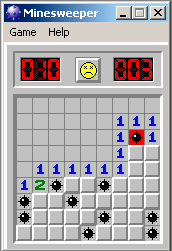
\includegraphics[scale=\FigScale]{examples/minesweeper/1.png}
\caption{\RU{Мины}\EN{Mines}}
\label{fig:minesweeper1}
\end{figure}

\RU{Сравнивая места с минами и дамп, мы можем обнаружить что 0x10 это граница, 0x0F\EMDASH{}пустой блок, 
0x8F\EMDASH{}мина.}
\EN{By comparing the mine places and the dump, we can conclude that 0x10 stands for border, 0x0F\EMDASH{}empty block, 0x8F---mine.}

\RU{Теперь я добавил комментариев и также включил все байты 0x8F в квадратные скобки:}
\EN{Now I added comments and also enclosed all 0x8F bytes into square brackets:}

\lstinputlisting{examples/minesweeper/2.lst}

\RU{Теперь я убрал все байты связанные с границами (0x10) и всё что за ними:}
\EN{Now I removed all \IT{border bytes} (0x10) and what's beyond those:}

\lstinputlisting{examples/minesweeper/3.lst}

\RU{Да, это всё мины, теперь это очень хорошо видно, в сравнении со скриншотом.}
\EN{Yes, these are mines, now it can be clearly seen and compared with the screenshot.}

\clearpage
\RU{Вот что интересно, это то что я могу модифицировать массив прямо в \olly.}
\EN{What is interesting is that I can modify the array right in \olly.}
\RU{Я убрал все мины заменив все байты 0x8F на 0x0F, и вот что у меня получилось в Сапёре}\EN{I removed 
all mines by changing all 0x8F bytes by 0x0F, and here is what I got in Minesweeper}:

\begin{figure}[H]
\centering
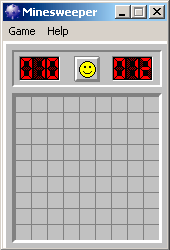
\includegraphics[scale=\FigScale]{examples/minesweeper/3.png}
\caption{\RU{Я убрал все мины в отладчике}\EN{I removed all mines in debugger}}
\label{fig:minesweeper3}
\end{figure}

\RU{Я также убрал их все и добавил их в первом ряду}\EN{I also moved all of them to the first line}: 

\begin{figure}[H]
\centering
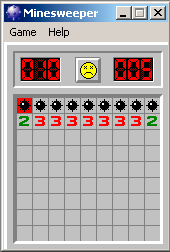
\includegraphics[scale=\FigScale]{examples/minesweeper/2.png}
\caption{\RU{Мины, установленные мною в отладчике}\EN{Mines I set in debugger}}
\label{fig:minesweeper2}
\end{figure}

\RU{Отладчик не очень удобен для подсматривания (а это была моя изначальная цель), так что я написал маленькую
утилиту для показа содержимого доски:}
\EN{Well, the debugger is not very convenient for eavesdropping (which was my goal anyway), so I wrote small utility
to dump the contents of the board:}

\lstinputlisting{examples/minesweeper/minesweeper_cheater.c}

\RU{Просто установите}\EN{Just set the} \ac{PID}
\footnote{PID \RU{можно увидеть в}\EN{it can be seen in} Task Manager 
(\RU{это можно включить в}\EN{enable it in} \q{View $\rightarrow$ Select Columns})} 
\RU{и адрес массива}\EN{and the address of the array} (\TT{0x01005340} \RU{для}\EN{for} Windows XP SP3 English) 
\RU{и она покажет его}\EN{and it will dump it}
\footnote{\RU{Скомпилированная версия здесь}\EN{The compiled executable is here}: 
\href{http://go.yurichev.com/17165}{beginners.re}}.

\RU{Она подключается к win32-процессу по \ac{PID}-у и просто читает из памяти процесса по этому адресу.}
\EN{It attaches itself to a win32 process by \ac{PID} and just reads process memory an the address.}

\section{\Exercises}

\begin{itemize}

\item \RU{Почему байты описывающие границы (0x10) присутствуют вообще?}
\EN{Why do the \IT{border bytes} (0x10) exist in the array?}
\RU{Зачем они нужны, если они вообще не видимы в интерфейсе Сапёра?}
\EN{What they are for if they are not visible in Minesweeper's interface?}
\RU{Как можно обойтись без них}\EN{How could it work without them}?

\item \RU{Как выясняется, здесь больше возможных значений (для открытых блоков, для тех на которых игрок установил
	флажок, \etc{}.).}
	\EN{As it turns out, there are more values possible (for open blocks, for flagged by user, \etc{}).}
\RU{Попробуйте найти значение каждого}\EN{Try to find the meaning of each one}.

\item \RU{Измените мою утилиту так, чтобы она в запущенном процессе Сапёра убирала все мины, 
или расставляла их в соответствии с каким-то заданным шаблоном.}
\EN{Modify my utility so it can remove all mines or set them in a fixed pattern that you want in the Minesweeper
process currently running.}

\item \RU{Измените мою утилиту так, чтобы она работала без задаваемого адреса массива и без \gls{PDB}-файла.}
\EN{Modify my utility so it can work without the array address specified and without a \gls{PDB} file.}
\RU{Да, вполне возможно автоматически найти информацию о доске в сегменте данных в запущенном процессе Сапёра.}
\EN{Yes, it's possible to find board information in the data segment of Minesweeper's running process automatically.}
\RU{Подсказка}\EN{Hint}: \myref{minesweeper_winxp_hint}.

\end{itemize}

\EN{\section{Hacking Windows clock}

Sometimes I did some kind of first April prank for my coworkers.

Let's find, if we could do something with Windows clock?
Can we force to go clock hands backwards?

First of all, when you click on date/time in status bar,\\
a \IT{C:\textbackslash{}WINDOWS\textbackslash{}SYSTEM32\textbackslash{}TIMEDATE.CPL} module gets executed,
which is usual executable PE file.

Let's see, how it draw hands?
When I open the file (from Windows 7) in Resource Hacker, there are clock faces, but with no hands:

\begin{figure}[H]
\centering
\myincludegraphics{examples/timedate/reshack.png}
\caption{Resource Hacker}
\end{figure}

OK, what we know? How to draw a clock hand? All they are started at the middle of circle, ending with its border.
Hence, we need to calculate coordinates of a point on circle's border.
From school-level mathematics we may remember that we need to use sine/cosine functions to draw circle, or at least
square root.
There are no such things in \IT{TIMEDATE.CPL}, at least at first glance.
But, thanks to Microsoft debugging PDB files, I can find a function named \IT{CAnalogClock::DrawHand()}, which calls
\IT{Gdiplus::Graphics::DrawLine()} at least twice.

Here is its code:

\lstinputlisting{examples/timedate/1.lst}

\myindex{Windows!Win32!MulDiv()}
We can see that \IT{DrawLine()} arguments are dependent on result of \IT{MulDiv()} function
and a \IT{table[]} table (name is mine),
which has 8-byte elements (look at \INS{LEA}'s second operand).

What is inside of table[]?

\lstinputlisting{examples/timedate/2.lst}

It's referenced only from \IT{DrawHand()} function at has 120 32-bit words or 60 32-bit pairs... wait, 60?
Let's take a closer look at these values.
First of all, I'll zap 6 pairs or 12 32-bit words with zeroes, and then I'll put patched \IT{TIMEDATE.CPL}
into \IT{C:\textbackslash{}WINDOWS\textbackslash{}SYSTEM32}.
(You may need to set owner of the *TIMEDATE.CPL* file to your primary user account (instead of \IT{TrustedInstaller}),
and also, boot in safe mode with command prompt so you can copy the file, which is usually locked.)

\begin{figure}[H]
\centering
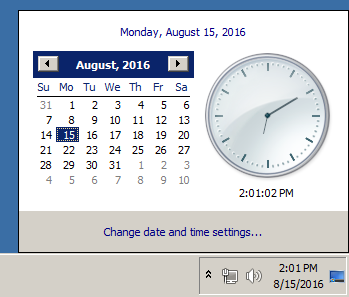
\includegraphics[width=0.5\textwidth]{examples/timedate/6_pairs_zeroed.png}
\caption{Attempt to run}
\end{figure}

Now when any hand is located at 0-5 seconds/minutes, it's invisible! However, opposite (shorter) part of second hand
is visible and moving.
When any hand is outside of this area, hand is visible as usual.

\myindex{Mathematica}
Let's take even closer look at the table in Mathematica.
I have copypasted table from the \IT{TIMEDATE.CPL} to a \IT{tbl} file (480 bytes).
We will take for granted the fact that these are signed values, because half of elements are below zero (0FFFFE0C1h, etc).
If these values would be unsigned, they would be suspiciously huge.

\begin{lstlisting}
In[]:= tbl = BinaryReadList["~/.../tbl", "Integer32"]

Out[]= {0, -7999, 836, -7956, 1663, -7825, 2472, -7608, 3253, -7308, 3999, \
-6928, 4702, -6472, 5353, -5945, 5945, -5353, 6472, -4702, 6928, \
-4000, 7308, -3253, 7608, -2472, 7825, -1663, 7956, -836, 8000, 0, \
7956, 836, 7825, 1663, 7608, 2472, 7308, 3253, 6928, 4000, 6472, \
4702, 5945, 5353, 5353, 5945, 4702, 6472, 3999, 6928, 3253, 7308, \
2472, 7608, 1663, 7825, 836, 7956, 0, 7999, -836, 7956, -1663, 7825, \
-2472, 7608, -3253, 7308, -4000, 6928, -4702, 6472, -5353, 5945, \
-5945, 5353, -6472, 4702, -6928, 3999, -7308, 3253, -7608, 2472, \
-7825, 1663, -7956, 836, -7999, 0, -7956, -836, -7825, -1663, -7608, \
-2472, -7308, -3253, -6928, -4000, -6472, -4702, -5945, -5353, -5353, \
-5945, -4702, -6472, -3999, -6928, -3253, -7308, -2472, -7608, -1663, \
-7825, -836, -7956}

In[]:= Length[tbl]
Out[]= 120
\end{lstlisting}

Let's treat two consecutive 32-bit values as pair:

\begin{lstlisting}
In[]:= pairs = Partition[tbl, 2]
Out[]= {{0, -7999}, {836, -7956}, {1663, -7825}, {2472, -7608}, \
{3253, -7308}, {3999, -6928}, {4702, -6472}, {5353, -5945}, {5945, \
-5353}, {6472, -4702}, {6928, -4000}, {7308, -3253}, {7608, -2472}, \
{7825, -1663}, {7956, -836}, {8000, 0}, {7956, 836}, {7825, 
1663}, {7608, 2472}, {7308, 3253}, {6928, 4000}, {6472, 
4702}, {5945, 5353}, {5353, 5945}, {4702, 6472}, {3999, 
6928}, {3253, 7308}, {2472, 7608}, {1663, 7825}, {836, 7956}, {0, 
7999}, {-836, 7956}, {-1663, 7825}, {-2472, 7608}, {-3253, 
7308}, {-4000, 6928}, {-4702, 6472}, {-5353, 5945}, {-5945, 
5353}, {-6472, 4702}, {-6928, 3999}, {-7308, 3253}, {-7608, 
2472}, {-7825, 1663}, {-7956, 836}, {-7999, 
0}, {-7956, -836}, {-7825, -1663}, {-7608, -2472}, {-7308, -3253}, \
{-6928, -4000}, {-6472, -4702}, {-5945, -5353}, {-5353, -5945}, \
{-4702, -6472}, {-3999, -6928}, {-3253, -7308}, {-2472, -7608}, \
{-1663, -7825}, {-836, -7956}}

In[]:= Length[pairs]
Out[]= 60
\end{lstlisting}

Let's try to treat each pair as X/Y coordinate and draw all 60 pairs, and also first 15 pairs:

\begin{figure}[H]
\centering
\myincludegraphics{examples/timedate/math.png}
\caption{Mathematica}
\end{figure}

Now this is something!
Each pair is just coordinate.
First 15 pairs are coordinates for $\frac{1}{4}$ of circle.

Perhaps, Microsoft developers precalculated all coordinates and put them into table.

Now I can understand why when I zapped 6 pairs, hands were invisible at that area: in fact, hands were drawed,
they just had zero length, because hand started at 0:0 coordinate and ended there.

\subsubsection{The prank (practical joke)}

Given all that, how would we force hands to go counterclockwise?
In fact, this is simple, we need just to rotate the table, so each hand, instead of drawing at place of first second,
would be drawing at place of 59th second.

I made the patcher a long time ago, at the very beginning of 2000s, for Windows 2000.
Hard to believe, it still works for Windows 7, perhaps, the table hasn't been changed since then!

Patcher source code: \url{https://github.com/dennis714/random_notes/blob/master/timedate/time_pt.c}.

Now I can see all hands goes backwards:

\begin{figure}[H]
\centering
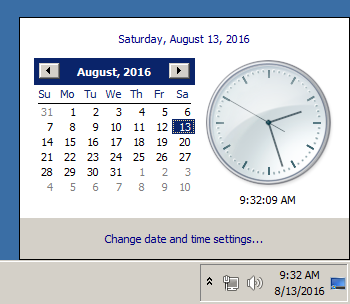
\includegraphics[width=0.5\textwidth]{examples/timedate/counterclockwise.png}
\caption{Now it works}
\end{figure}

Well, there is no animation in this article, but if you look closer, you can see, that hands are in fact shows correct
time, but the whole clock face is rotated vertically, like we see it from the inside of clock.

\subsubsection{Windows 2000 leaked source code}

So I did the patcher and then Windows 2000 source code has been leaked (I can't force you to trust me, though).
Let's take a look on source code if that function and table.\\
The file is \IT{win2k/private/shell/cpls/utc/clock.c}:

\begin{lstlisting}
//
//  Array containing the sine and cosine values for hand positions.
//
POINT rCircleTable[] =
{
    { 0,     -7999},
    { 836,   -7956},
    { 1663,  -7825},
    { 2472,  -7608},
    { 3253,  -7308},
...
    { -4702, -6472},
    { -3999, -6928},
    { -3253, -7308},
    { -2472, -7608},
    { -1663, -7825},
    { -836 , -7956},
};

////////////////////////////////////////////////////////////////////////////
//
//  DrawHand
//
//  Draws the hands of the clock.
//
////////////////////////////////////////////////////////////////////////////

void DrawHand(
    HDC hDC,
    int pos,
    HPEN hPen,
    int scale,
    int patMode,
    PCLOCKSTR np)
{
    LPPOINT lppt;
    int radius;

    MoveTo(hDC, np->clockCenter.x, np->clockCenter.y);
    radius = MulDiv(np->clockRadius, scale, 100);
    lppt = rCircleTable + pos;
    SetROP2(hDC, patMode);
    SelectObject(hDC, hPen);

    LineTo( hDC,
            np->clockCenter.x + MulDiv(lppt->x, radius, 8000),
            np->clockCenter.y + MulDiv(lppt->y, radius, 8000) );
}
\end{lstlisting}

Now it's clear: coordinates has been precalculated as if clock face has height and width of $2 \cdot 8000$,
and then it's rescaled to current clock face radius using \IT{MulDiv()} function.

POINT structure\footnote{\url{https://msdn.microsoft.com/en-us/library/windows/desktop/dd162805(v=vs.85).aspx}}
is a structure of two 32-bit values, first is \IT{x}, second is \IT{y}.

}
\chapterold{\RU{Донглы}\EN{Dongles}}
\label{dongles}

\RU{Автор этих строк иногда делал замену \glslink{dongle}{донглам} или \q{эмуляторы донглов} 
и здесь немного примеров, как это происходит.}
\EN{The author of these lines, occasionally did software copy-protection \gls{dongle} replacements, or \q{dongle emulators} and here
are couple examples of how it's happening.}

\RU{Об одном неописанном здесь случае с Rockey и Z3 вы также можете прочитать здесь}
\EN{About one of the cases about Rocket and Z3 that is not present here, you can read here}:
\url{http://yurichev.com/tmp/SAT_SMT_DRAFT.pdf}.

\subsection{\IFRU{Пример}{Example} \#1: MacOS Classic \AndENRU PowerPC}

\index{PowerPC}
\index{Mac OS Classic}
\IFRU{Как-то я получил программу для}{I've got a program for} MacOS Classic
\footnote{\IFRU{MacOS перед тем как перейти на UNIX}{pre-UNIX MacOS}}, \IFRU{для}{for} PowerPC.
\IFRU{Компания, разработавшая этот продукт давно исчезла, так что (легальный) пользователь
боялся того что донгла может сломаться}{The company who developed the software product
was disappeared long time ago, so the (legal) customer was afraid of physical dongle damage}.

\IFRU{Если запустить программу без подключенной донглы, можно увидеть окно с надписью}
{While running without dongle connected, a message box with a text}
"Invalid Security Device"\IFRU{}{ appeared}.
\IFRU{Мне повезло потому что этот текст можно было легко найти внутри исполняемого файла}
{Luckily, this text string can be found easily in the executable binary file}.

\IFRU{Я не был знаком ни с Mac OS Classic, ни с PowerPC, но решил попробовать}
{I was not very familiar both with Mac OS Classic and PowerPC, but I tried anyway}.

\ac{IDA} \IFRU{открывает исполняемый файл легко, показывая его тип как}
{opens the executable file smoothly, reported its type as} 
"PEF (Mac OS or Be OS executable)" (\IFRU{действительно, это стандартный тип файлов в Mac OS Classic}
{indeed, it is a standard Mac OS Classic file format}).

\IFRU{В поисках текстовой строки с сообщение об ошибке, я попал на этот фрагмент кода}
{By searching for the text string with error message, I've got into this code fragment}:

\lstinputlisting{examples/dongles/1/1.lst}

\index{ARM}
\index{MIPS}
\IFRU{Да, это код PowerPC}{Yes, this is PowerPC code}.
\IFRU{Это очень типичный процессор для \ac{RISC} 1990-х}
{The CPU is very typical 32-bit \ac{RISC} of 1990s era}.
\IFRU{Каждая инструкция занимает 4 байта (как и в MIPS и ARM) и их имена немного похожи на имена 
инструкций MIPS}
{Each instruction occupies 4 bytes (just as in MIPS and ARM) and its names are somewhat resembling
MIPS instruction names}.

\TT{check1()} \IFRU{это имя которое я дал этой ф-ции позже}{is a function name I gave it to lately}.
\TT{BL} \IFRU{это инструкция}{is} \IT{Branch Link} 
\IFRU{т.е., предназначенная для вызова подпрограмм}{instruction, e.g., intended for subroutines calling}.
\IFRU{Самое важное место ~--- это инструкция \ac{BNE} срабатывающая если проверка наличия донглы прошла
успешно, либо не срабатывающая в случае ошибки: и тогда адрес текстовой строки с сообщением об ошибке
будет загружен в регистр r3 для последующей передачи в функцию отображения диалогового окна}
{The crucial point is \ac{BNE} instruction jumping if dongle protection check is passed 
or not jumping if error is occurred: 
then the address of the text string being loaded into r3 register for the subsequent passage into message box routine}.

\IFRU{Из}{From the} \cite{PPCABI} \IFRU{я узнал, что регистр r3 используется для возврата
значений (и еще r4 если значение 64-битное)}
{I've got to know the r3 register is used for values returning (and r4, in case of 64-bit values)}.

\index{x86!\Instructions!MOVZX}
\IFRU{Еще одна пока что неизвестная инструкция}{Another yet unknown instruction is} \TT{CLRLWI}. 
\IFRU{Из}{From} \cite{PPC} \IFRU{я узнал, что эта инструкция одновременно и очищает и загружает}{I've got to know that this instruction
do both clearing and loading}. 
\IFRU{В нашем случае, она очищает 24 старших бита из значения в r3 и записывает всё это в r0, 
так что это аналог}{In our case, it clears 24 high bits from the value in r3
and put it to r0, so it is analogical to} \MOVZX \InENRU x86 (\ref{movzx}),
\IFRU{но также устанавливает флаги, так что}{but it also sets the flags, so the} \ac{BNE} 
\IFRU{может проверить их потом}{can check them after}.

\IFRU{Посмотрим внутрь}{Let's take a look into} \TT{check1()}\IFRU{}{ function}:

\lstinputlisting{examples/dongles/1/check1.lst}

\IFRU{Как можно увидеть в \ac{IDA}, эта ф-ция вызывается из многих мест в программе, но только значение
в регистре r3 проверяется сразу после каждого вызова}
{As I can see in \ac{IDA}, that function is called from many places in program, but only r3 register value
is checked right after each call}.
\index{thunk-\IFRU{функции}{functions}}
\IFRU{Всё что эта ф-ция делает это только вызывает другую ф-цию, так что это}
{All this function does is calling other function, so it is} \gls{thunk function}: 
\IFRU{здесь присутствует и пролог ф-ции и эпилог, но регистр r3 не трогается, так что}
{there is function prologue and epilogue, but r3 register is not touched, so} \TT{checkl()} 
\IFRU{возвращает то, что возвращает}{returns what} \TT{check2()}\IFRU{}{ returns}.

\ac{BLR} \IFRU{это похоже возврат из ф-ции, но так как IDA делает всю разметку ф-ций автоматически,
наверное, мы можем пока не интересоваться этим}{is seems return from function, but since \ac{IDA} does functions layout, we probably do not need
to be interesting in this}.
\IFRU{Так как это типичный \ac{RISC}, похоже, подпрограммы вызываются используя}
{It seems, since it is a typical \ac{RISC}, subroutines are called using} \gls{link register},
\IFRU{точно как в}{just like in} ARM.

\IFRU{Ф-ция }{}\TT{check2()} \IFRU{более сложная}{function is more complex}:

\lstinputlisting{examples/dongles/1/check2.lst}

\IFRU{Снова повезло: имена некоторых ф-ций оставлены в исполняемом файле
(в символах в отладочной секции? Я не уверен, т.к. я не знаком с этим форматом файлов,
может быть это что-то вроде PE-экспортов (\ref{PE_exports_imports}))?
как например \TT{.RBEFINDNEXT()} and \TT{.RBEFINDFIRST()}.}
{I'm lucky again: some function names are leaved in the executable 
(debug symbols section? I'm not sure, since I'm not very familiar with the file format, maybe it is
some kind of PE exports? (\ref{PE_exports_imports})),
like \TT{.RBEFINDNEXT()} and \TT{.RBEFINDFIRST()}.}
\IFRU{В итоге, эти ф-ции вызывают другие ф-ции с именами вроде}
{Eventually these functions are calling other functions with names like} \TT{.GetNextDeviceViaUSB()}, 
\TT{.USBSendPKT()},
\IFRU{так что они явно работают с каким-то USB-устройством}{so these are clearly dealing with USB device}.

\IFRU{Тут даже есть ф-ция с названием}{There are even a function named} 
\TT{.GetNextEve3Device()}\EMDASH\IFRU{звучит знакомо, в 1990-х годах была донгла}{sounds familiar, there was} Sentinel Eve3 
\IFRU{для ADB-порта (присутствующих на Макинтошах)}{dongle for ADB port (present on Macs) in 1990s}.

\IFRU{В начале посмотрим на то как устанавливается регистр r3 одновременно игнорируя всё остальное}
{Let's first take a look on how r3 register is set before return simultaneously ignoring all we see}.
\IFRU{Мы знаем, что ``хорошее'' значение в r3 должно быть не нулевым, а нулевой r3 приведет
к выводу диалогового окна с сообщением об ошибке}
{We know that ``good'' r3 value should be non-zero, zero r3 will lead execution
flow to the message box with an error message}.

\IFRU{В ф-ции имеются две инструкции}{There are two instructions} \TT{li \%r3, 1} 
\IFRU{и одна}{present in the function and one} \TT{li \%r3, 0} 
(\IT{Load Immediate}, \IFRU{т.е., загрузить значение в регистр}{i.e., loading value into register}).
\IFRU{Самая первая инструкция находится на}{The very first instruction at} 
\TT{0x001186B0}\EMDASH\IFRU{и честно говоря, я не знаю что это означает, нужно больше времени на изучение ассемблера PowerPC}
{frankly speaking, I don't know
what it mean, I need some more time to learn PowerPC assembly language}.

\IFRU{А вот то что мы видим дальше понять проще}{What we see next is, however, easier to understand}: 
\IFRU{вызывается }{}\TT{.RBEFINDFIRST()} \IFRU{и в случае ошибки, 0 будет записан в r3
и мы перейдем на \IT{exit}, а иначе будет вызвана ф-ция \TT{check3()} ~--- если и она будет
выполнена с ошибкой, будет вызвана}{is called:
in case of its failure, 0 is written into r3 and we jump to \IT{exit}, otherwise another
function is called (\TT{check3()})~---if it is failing too, 
the} \TT{.RBEFINDNEXT()} \IFRU{вероятно, для поиска другого USB-устройства}
{is called, probably, in order to look for another USB device}.

N.B.: \TT{clrlwi. \%r0, \%r3, 16} \IFRU{это аналог того что мы уже видели, но она очищает 16 старших бит,
т.е.}{it is analogical to what we already saw, but it clears
16 bits, i.e.}, \TT{.RBEFINDFIRST()} \IFRU{вероятно возвращает 16-битное значение}
{probably returns 16-bit value}.

\TT{B} \IFRU{означает}{meaning} \IT{branch} \IFRU{~--- безусловный переход}{is unconditional jump}.

\ac{BEQ} \IFRU{это обратная инструкция от}{is inverse instruction of} \ac{BNE}.

\IFRU{Посмотрим на}{Let's see} \TT{check3()}:

\lstinputlisting{examples/dongles/1/check3.lst}

\IFRU{Здесь много вызовов}{There are a lot of calls to} \TT{.RBEREAD()}. 
\IFRU{Эта ф-ция вероятно читает какие-то значения из донглы, которые потом сравниваются здесь при помощи}
{The function is probably return some values from the dongle,
so they are compared here with hard-coded variables using} \TT{CMPLWI}.

\IFRU{Мы также видим в регистр r3 записывается перед каждым вызовом}
{We also see that r3 register is also filled before each call to} \TT{.RBEREAD()} 
\IFRU{одно из этих значений}{by one of these values}: 0, 1, 8, 0xA, 0xB, 0xC, 0xD, 4, 5.
\IFRU{Вероятно адрес в памяти или что-то в этом роде}{Probably memory address or something like that}?

\IFRU{Да, действительно, если погуглить имена этих ф-ций, можно легко найти документацию к}
{Yes, indeed, by googling these function names it is easy to find} Sentinel Eve3\IFRU{}{ dongle manual}!

\IFRU{Мне даже, наверное, не нужно изучать остальные инструкции PowerPC: всё что делает эта ф-ция это просто
вызывает}
{I probably even do not need to learn other PowerPC instructions: all this function does is just
calls} \TT{.RBEREAD()}, \IFRU{сравнивает его результаты с константами и возвращает 1 если результат сравнения положительный или 0 в другом случае}{compare its results with constants and returns 1 if comparisons
are fine or 0 otherwise}.

\IFRU{Всё ясно: \TT{check1()} должна всегда возвращать 1 или иное ненулевое значение}
{OK, all we've got is that \TT{check1()} should return always 1 or any other non-zero value}.
\IFRU{Но так как я не очень уверен в своих знаниях инструкций PowerPC, я буду осторожен и пропатчу
переходы в \TT{check2} на адресах}{But since I'm not very confident in PowerPC instructions,
I will be careful: I will patch
jumps in \TT{check2()} at} \TT{0x001186FC} \AndENRU \TT{0x00118718}.

\IFRU{На}{At} \TT{0x001186FC} \IFRU{я записал байты}{I wrote bytes} 0x48 \AndENRU 0 
\IFRU{таким образом превращая инструкцию}{thus converting} \ac{BEQ} 
\IFRU{в инструкцию}{instruction into} 
\TT{B} (\IFRU{безусловный переход}{unconditional jump}):
\IFRU{Я заметил этот опкод прямо в коде даже без обращения к}
{I spot its opcode in the code without even referring to} \cite{PPC}.

\IFRU{На}{At} \TT{0x00118718} \IFRU{я записал байт}{I wrote} 0x60 \AndENRU \IFRU{еще 3 нулевых байта,
таким образом превращая её в инструкцию}{3 zero bytes thus converting it to}
\ac{NOP}\IFRU{}{ instruction}:
\IFRU{Этот опкод я тоже подсмотрел прямо в коде}{I spot its opcode in the code too}.

\IFRU{Резюмируя, такие простые модификации можно делать в \ac{IDA} даже с минимальными знаниями
ассемблера}{Summarizing, such small modifications can be done with \ac{IDA} and minimal assembly language knowledge}.


\EN{\subsection{Example \#2: SCO OpenServer}

\label{examples_SCO}
\myindex{SCO OpenServer}
An ancient software for SCO OpenServer from 1997 
developed
by a company that disappeared a long time ago.


There is a special dongle driver to be installed in the system, that contains the following text strings:
\q{Copyright 1989, Rainbow Technologies, Inc., Irvine, CA}
\AndENRU
\q{Sentinel Integrated Driver Ver. 3.0 }.


After the installation of the driver in SCO OpenServer, these device files appear in the /dev filesystem:

\begin{lstlisting}
/dev/rbsl8
/dev/rbsl9
/dev/rbsl10
\end{lstlisting}


The program reports an error without dongle connected, but the error string cannot be found in the executables.

\myindex{COFF}

Thanks to \ac{IDA}, it is easy to load the COFF executable used in SCO OpenServer.

%
Let's also try to find \q{rbsl} string and indeed, found it in this code fragment:

\lstinputlisting{examples/dongles/2/1.lst}


Yes, indeed, the program needs to communicate with the driver somehow.

\myindex{thunk-functions}
The only place where the \TT{SSQC()}
function is called is the \gls{thunk function}:

\lstinputlisting{examples/dongles/2/2.lst}

SSQ() 
is called from at least 2 functions.

One of these is:

\lstinputlisting{examples/dongles/2/check1.lst}

\q{\TT{3C}} \AndENRU \q{\TT{3E}} 
sound familiar: there was a Sentinel Pro dongle by Rainbow with no memory,
providing only one crypto-hashing secret function.

You can read a short description
of what hash function is here: \myref{hash_func}.

But let's get back to the program.

So the program can only check the presence or absence of a connected dongle.

No other information can be written to such dongle, as it has no memory.
The two-character codes are commands
(we can see how the commands are handled in the 
\TT{SSQC()} function) 

and all other strings are hashed inside the dongle, being transformed into a 16-bit number.
The algorithm was secret,
so it was not possible to write a driver replacement or to remake the dongle hardware that would emulate it perfectly.

However, it is always possible to intercept all accesses to it and to find what constants
the hash function results are compared to.

But we need to say that it is possible to build a robust software copy protection scheme based on secret
cryptographic hash-function: let it encrypt/decrypt the data files your software uses.

But let's get back to the code.

Codes 51/52/53 
are used for LPT printer port selection.
3x/4x are used for \q{family} 
selection (that's how Sentinel Pro dongles are differentiated from each other: more than one
dongle can be connected to a LPT port).


The only non-2-character string passed to the hashing function is "0123456789".

Then, the result is compared against the set of valid results.

If it is correct, 0xC or 0xB is to be written into the global variable \TT{ctl\_model}.%


Another text string that gets passed is
"PRESS ANY KEY TO CONTINUE: ", but the result is not checked.
Hard to say why, probably by mistake
\footnote{
What a strange feeling: to find bugs in such ancient software.}.


Let's see where the value from the global variable \TT{ctl\_mode} is used.

One such place is:

\lstinputlisting{examples/dongles/2/4.lst}

If it is 0, an encrypted error message is passed to a decryption routine and printed.

\myindex{x86!\Instructions!XOR}

The error string decryption routine seems a simple \gls{xoring}:

\lstinputlisting{examples/dongles/2/err_warn.lst}

%
That's why we were unable to find the error messages in the executable files, because they are encrypted
(which is is popular practice).

Another call to the \TT{SSQ()} hashing function passes the
\q{offln} string to it and compares the result with
\TT{0xFE81} \AndENRU \TT{0x12A9}.

If they don't match, it works with some \TT{timer()} 
function (maybe waiting for a poorly
connected dongle to be reconnected and check again?) and then decrypts another error message to dump.

\lstinputlisting{examples/dongles/2/check2.lst}

Bypassing the dongle is pretty straightforward: just patch all jumps after the relevant \CMP instructions.


Another option is to write our own SCO OpenServer driver, containing a table of questions and answers, all of those which present in the program.

\subsubsection{Decrypting error messages}

By the way, we can also 
try to decrypt all error messages.
The algorithm that is located in the \TT{err\_warn()} 
function is very simple, indeed:

\lstinputlisting[caption=Decryption function]{examples/dongles/2/decrypting_EN.lst}

As we can see, 
not just string is supplied to the decryption function, but also the key:

\begin{lstlisting}
.text:0000DAF7 error:                                  ; CODE XREF: sync_sys+255j
.text:0000DAF7                                         ; sync_sys+274j ...
.text:0000DAF7                 mov     [ebp+var_8], offset encrypted_error_message2
.text:0000DAFE                 mov     [ebp+var_C], 17h ; decrypting key
.text:0000DB05                 jmp     decrypt_end_print_message

...

; this name we gave to label manually:
.text:0000D9B6 decrypt_end_print_message:              ; CODE XREF: sync_sys+29Dj
.text:0000D9B6                                         ; sync_sys+2ABj
.text:0000D9B6                 mov     eax, [ebp+var_18]
.text:0000D9B9                 test    eax, eax
.text:0000D9BB                 jnz     short loc_D9FB
.text:0000D9BD                 mov     edx, [ebp+var_C] ; key
.text:0000D9C0                 mov     ecx, [ebp+var_8] ; string
.text:0000D9C3                 push    edx
.text:0000D9C4                 push    20h
.text:0000D9C6                 push    ecx
.text:0000D9C7                 push    18h
.text:0000D9C9                 call    err_warn
\end{lstlisting}

The algorithm is a simple \gls{xoring}: 
each 
byte is xored with a key, but the key is increased by 3 after the processing of each byte.

We can write a simple Python script to check our hypothesis:

\lstinputlisting[caption=Python 3.x]{examples/dongles/2/decr1.py}

And it prints: \q{check security device connection}.
So yes, this is the decrypted message.

There are also 
other encrypted messages with their corresponding keys.
But needless to say, it is possible 
to decrypt them without their keys.
First, we can see that the key 
is in fact a byte.
It is because the core decryption instruction
(\XOR) works on byte level. 
The key is located in the \ESI register, but only one byte part of \ESI is used.
Hence, a key may be greater than 255, 
but its value is always to be rounded.


As a consequence, we can just try brute-force, trying all possible keys in the 0..255 range.
We are also going to skip 
the messages that contain unprintable characters.

\lstinputlisting[caption=Python 3.x]{examples/dongles/2/decr2.py}

And we get:

\lstinputlisting[caption=Results]{examples/dongles/2/decr2_result.txt}

There 
is some garbage, but we can quickly find the English-language messages!

By the way, since the algorithm is a simple xoring encryption, the very same function can be used
to encrypt messages.
If needed, we can encrypt our own messages, and patch the program by inserting them.

}
\RU{\sectionold{Пример \#2: SCO OpenServer}

\label{examples_SCO}
\myindex{SCO OpenServer}
Древняя программа для SCO OpenServer от 1997 
разработанная давно исчезнувшей компанией.

Специальный драйвер донглы инсталлируется в системе, он содержит такие текстовые строки
:
\q{Copyright 1989, Rainbow Technologies, Inc., Irvine, CA}
\AndENRU
\q{Sentinel Integrated Driver Ver. 3.0 }.

После инсталляции драйвера, в /dev появляются такие устройства
:

\begin{lstlisting}
/dev/rbsl8
/dev/rbsl9
/dev/rbsl10
\end{lstlisting}

Без подключенной донглы, программа сообщает об ошибке, но сообщение об ошибке не удается
найти в исполняемых файлах
.

\myindex{COFF}
Еще раз спасибо \ac{IDA}, она легко загружает исполняемые файлы формата COFF использующиеся в
 SCO OpenServer.

Попробуем также поискать строку \q{rbsl}, и действительно, её можно найти в таком фрагменте кода%
:

\lstinputlisting{examples/dongles/2/1.lst}

Действительно, должна же как-то программа обмениваться информацией с драйвером
.

\myindex{thunk-функции}
Единственное место где вызывается функция \TT{SSQC()}
это \gls{thunk function}:

\lstinputlisting{examples/dongles/2/2.lst}

А вот SSQ() вызывается по крайней мере из двух разных функций
.

Одна из них:

\lstinputlisting{examples/dongles/2/check1.lst}

\q{\TT{3C}} \AndENRU \q{\TT{3E}} \EMDASH{}это звучит знакомо: когда-то была донгла
 Sentinel Pro от Rainbow без памяти,
предоставляющая только одну секретную крипто-хеширующую функцию.

О том, что такое хэш-функция, было описано здесь: \myref{hash_func}.

Но вернемся к нашей программе.
Так что программа может только проверить подключена ли донгла или нет
.
Никакой больше информации в такую донглу без памяти записать нельзя
.
Двухсимвольные коды\EMDASH{}это команды
(можно увидеть, как они обрабатываются в функции 
\TT{SSQC()}) 
а все остальные строки хешируются внутри донглы превращаясь в 16-битное число
.
Алгоритм был секретный, так что нельзя было написать замену драйверу или сделать
электронную копию донглы идеально эмулирующую алгоритм.
С другой стороны, всегда можно было перехватить все обращения к ней и найти те константы, с которыми
сравнивается результат хеширования
.
Но надо сказать, вполне возможно создать устойчивую защиту от копирования базирующуюся
на секретной хеш-функции: пусть она шифрует все файлы с которыми ваша программа работает
.

Но вернемся к нашему коду.

Коды 51/52/53 используются для выбора номера принтеровского LPT-порта
.
3x/4x используются для выбора \q{family} так донглы Sentinel Pro
можно отличать друг от друга: ведь более одной донглы может быть подключено к LPT-порту
.

Единственная строка, передающаяся в хеш-функцию это
 "0123456789".
Затем результат сравнивается с несколькими правильными значениями
.

%
Если результат правилен, 0xC или 0xB будет записано в глобальную переменную \TT{ctl\_model}.

Еще одна строка для хеширования:
"PRESS ANY KEY TO CONTINUE: ", но результат не проверяется.
Трудно сказать, зачем это, может быть по ошибке
\footnote{Это очень странное чувство: находить ошибки в столь древнем ПО.
}.

Давайте посмотрим, где проверяется значение глобальной переменной
 \TT{ctl\_mode}.

Одно из таких мест:

\lstinputlisting{examples/dongles/2/4.lst}

Если оно 0, шифрованное сообщение об ошибке будет передано в функцию дешифрования, и оно будет 
показано.

\myindex{x86!\Instructions!XOR}
Функция дешифровки сообщений об ошибке похоже применяет простой \gls{xoring}
:

\lstinputlisting{examples/dongles/2/err_warn.lst}

Вот почему не получилось найти сообщение об ошибке в исполняемых файлах, потому что оно было
зашифровано, это очень популярная практика%
.

Еще один вызов хеширующей функции передает строку
\q{offln} и сравнивает результат с константами
\TT{0xFE81} \AndENRU \TT{0x12A9}.
Если результат не сходится, происходит работа с какой-то функцией
 \TT{timer()} 
(может быть для ожидания плохо подключенной донглы и нового запроса?), затем дешифрует
еще одно сообщение об ошибке и выводит его.

\lstinputlisting{examples/dongles/2/check2.lst}

Заставить работать программу без донглы довольно просто: просто пропатчить все места после инструкций
\CMP где происходят соответствующие сравнения.

Еще одна возможность\EMDASH{}это написать свой драйвер для SCO OpenServer, содержащий таблицу возможных вопросов и ответов, все те что имеются в програме.


\subsectionold{Дешифровка сообщений об ошибке}

Кстати, мы также можем дешифровать все сообщения об ошибке.
Алгоритм, находящийся в функции \TT{err\_warn()} 
действительно, крайне прост:

\lstinputlisting[caption=Функция дешифровки]{examples/dongles/2/decrypting_RU.lst}

Как видно, не только сама строка поступает на вход, но также и ключ для дешифровки:

\begin{lstlisting}
.text:0000DAF7 error:                                  ; CODE XREF: sync_sys+255j
.text:0000DAF7                                         ; sync_sys+274j ...
.text:0000DAF7                 mov     [ebp+var_8], offset encrypted_error_message2
.text:0000DAFE                 mov     [ebp+var_C], 17h ; decrypting key
.text:0000DB05                 jmp     decrypt_end_print_message

...

; this name we gave to label manually:
.text:0000D9B6 decrypt_end_print_message:              ; CODE XREF: sync_sys+29Dj
.text:0000D9B6                                         ; sync_sys+2ABj
.text:0000D9B6                 mov     eax, [ebp+var_18]
.text:0000D9B9                 test    eax, eax
.text:0000D9BB                 jnz     short loc_D9FB
.text:0000D9BD                 mov     edx, [ebp+var_C] ; key
.text:0000D9C0                 mov     ecx, [ebp+var_8] ; string
.text:0000D9C3                 push    edx
.text:0000D9C4                 push    20h
.text:0000D9C6                 push    ecx
.text:0000D9C7                 push    18h
.text:0000D9C9                 call    err_warn
\end{lstlisting}

Алгоритм это очень простой \gls{xoring}: 
каждый байт XOR-ится с ключом, но ключ увеличивается на 3 после обработки каждого байта.

Напишем небольшой скрипт на Python для проверки наших догадок:

\lstinputlisting[caption=Python 3.x]{examples/dongles/2/decr1.py}

И он выводит: \q{check security device connection}.
Так что да, это дешифрованное сообщение.

Здесь есть также и другие сообщения, с соответствующими ключами.
Но надо сказать, их можно дешифровать и без ключей.
В начале, мы можем заметить, что ключ\EMDASH{}это просто байт.
Это потому что самая важная часть функции дешифровки
(\XOR) оперирует байтами. 
Ключ находится в регистре \ESI, но только младшие 8 бит
(т.е. байт) регистра используются.
Следовательно, ключ может быть больше 255, 
но его значение будет округляться.

И как следствие, мы можем попробовать обычный перебор всех ключей в диапазоне
 0..255.
Мы также можем пропускать сообщения содержащие непечатные символы.

\lstinputlisting[caption=Python 3.x]{examples/dongles/2/decr2.py}

И мы получим:

\lstinputlisting[caption=Results]{examples/dongles/2/decr2_result.txt}

Тут есть какой-то мусор, но мы можем быстро отыскать сообщения на английском языке!

Кстати, так как алгоритм использует простой \XOR, та же функция может использоваться и для шифрования
сообщения.
Если нужно, мы можем зашифровать наши собственные сообщения, и пропатчить программу вставив
их.

}
\subsection{\IFRU{Пример}{Example} \#3: MS-DOS}

\index{MS-DOS}
\IFRU{Еще одна очень старая программа для}{Another very old software for} MS-DOS \IFRU{от}{from} 1995 
\IFRU{также разработанная давно исчезнувшей компанией}
{also developed by a company disappeared long time ago}.

\index{8086}
\index{80286}
\IFRU{Во времена перед DOS-экстендерами, всё ПО для MS-DOS расчитывалось на процессоры 8086 или 80286,
так что в своей массе весь код был 16-битным}
{In the pre-DOS extenders era, all the software for MS-DOS were mostly rely on 16-bit 8086 or 80286 CPUs,
so en masse code was 16-bit}.
\IFRU{16-битный код в основном такой же, какой вы уже видели в этой книге, но все регистры 16-битные,
и доступно меньше инструкций}
{16-bit code is mostly same as you already saw in this book, but all registers
are 16-bit and there are less number of instructions available}.

\label{IN_example}
\label{OUT_example}
\index{x86!\Instructions!IN}
\index{x86!\Instructions!OUT}
\IFRU{Среда MS-DOS не могла иметь никаких драйверов, и ПО работало с ``голым'' железом через порты,
так что здесь вы можете увидеть инструкции \TT{OUT}/\TT{IN}, 
которые в наше время присутствуют в основном только
в драйверах (в современных OS нельзя обращаться на прямую к портам из \gls{user mode})}
{MS-DOS environment has no any system drivers, any program may deal with bare hardware via ports,
so here you may see \TT{OUT}/\TT{IN} instructions, which are mostly present in drivers in our times
(it is not possible to access ports directly in \gls{user mode} in all modern OS)}.

\IFRU{Учитывая это, ПО для MS-DOS должно работать с донглой обращаясь к принтерному LPT-порту
напрямую}
{Given that, the MS-DOS program working with a dongle should access LPT printer port directly}.
\IFRU{Так что мы можем просто поискать эти инструкции. И да, вот они}
{So we can just search for such instructions. And yes, here it is}:

\lstinputlisting{examples/dongles/3/1.lst}

(\IFRU{Все имена меток в этом примере даны мною}{All label names in this example were given by me}).

\IFRU{Функция }{}\TT{out\_port()} \IFRU{вызывается только из одной ф-ции}
{is referenced only in one function}:

\lstinputlisting{examples/dongles/3/2.lst}

\IFRU{Это также ``хеширующая'' донгла Sentinel Pro как и в предыдущем примере}
{It is also Sentinel Pro ``hashing'' dongle as in the previous example}.
\IFRU{Я заметил это по тому что текстовые строки передаются и здесь, 
16-битные значения также возвращаются и сравниваются с другими}
{I figured out its type by noticing that a text strings are also passed here and 16 bit values
are also returned and compared with others}.

\IFRU{Так вот как происходит работа с Sentinel Pro через порты}
{So that is how Sentinel Pro is accessed via ports}.
\IFRU{Адрес выходного порта обычно 0x378, т.е., принтерного порта, данные для него во времена
перед USB отправлялись прямо сюда}
{Output port address is usually 0x378, i.e.,
printer port, the data to the old printers in pre-USB era were passed to it}.
\IFRU{Порт однонаправленный, потому что когда его разрабатывали, никто не мог предположить
что кому-то понадобится получать информацию из принтера}
{The port is one-directional, because when it was developed, no one can imagined someone
will need to transfer information from the printer}
\footnote{\IFRU{Если учитывать только Centronics и не учитывать последующий стандарт IEEE 1284 ~---
в нем из принтера можно получать информацию}
{If to consider Centronics only. Following IEEE 1284 standard allows to transfer information from
the printer}.}.
\IFRU{Единственный способ получить информацию из принтера это регистр статуса на порту 0x379,
он содержит такие биты как ``paper out'', ``ack'', ``busy'' ~--- так принтер может сигнализировать
о том что он готов или нет, и о том, есть ли в нем бумага}
{The only way to get information from the printer, is a status register on port 0x379, it contain
such bits as ``paper out'', ``ack'', ``busy''~---thus printer may signal to the host computer
that it is ready or not and if a paper present in it}.
\IFRU{Так что донгла возвращает информацию через какой-то из этих бит, по одному биту на каждой
итерации}
{So the dongle return information from one of these bits, by one bit at each iteration}.

\TT{\_in\_port\_2} \IFRU{содержит адрес статуса}{has address of status word} (0x379) \AndENRU 
\TT{\_in\_port\_1} \IFRU{содержит адрес управляющего регистра}{has control register address} (0x37A).

\IFRU{Судя по всему, донгла возвращает информацию только через флаг ``busy'' на}
{It seems, the dongle return information via ``busy'' flag at} \TT{seg030:00B9}: 
\IFRU{каждый бит записывается в регистре \TT{DI} позже возвращаемый в самом конце ф-ции}
{each bit is stored in the \TT{DI} register, later returned at the function end}.

\IFRU{Что означают все эти отсылаемые в выходной порт байты}
{What all these bytes sent to output port mean}?
\IFRU{Я не знаю. Возможно, команды донглы.}
{I don't know. Probably commands to the dongle.}
\IFRU{Но честно говоря, нам и не обязательно знать: нашу задачу можно легко решить и без этих знаний}
{But generally speaking, it is not necessary to know: it is easy to solve our task without that knowledge}.

\IFRU{Вот ф-ция проверки донглы}{Here is a dongle checking routine}:

\lstinputlisting{examples/dongles/3/3.lst}

\IFRU{А так как эта ф-ция может вызываться слишком часто, например, 
перед выполнением каждой важной фичи ПО,
а обращение к донгле вообще-то медленное (и из-за медленного принтерного порта и из-за медленного
\ac{MCU} в донгле), так что они наверное добавили возможность пропускать проверку донглы слишком часто,
используя текущее время в ф-ции \TT{biostime()}}
{Since the routine may be called too frequently, e.g., before each important software feature executing, 
and the dongle accessing process is generally slow (because of slow printer port and also slow
\ac{MCU} in the dongle), so they probably added a way to skip dongle checking too often,
using checking current time in \TT{biostime()} function}.

\index{\CStandardLibrary!rand()}
\IFRU{Ф-ция }{}\TT{get\_rand()} \IFRU{использует стандартную ф-цию Си}
{function uses standard C function}:

\lstinputlisting{examples/dongles/3/4.lst}

\IFRU{Так что текстовая строка выбирается случайно, отправляется в донглу и результат
хеширования сверяется с корректным значением}
{So the text string is selected randomly, passed into dongle, and then the result of hashing 
is compared with correct value}.

\IFRU{Текстовые строки, похоже, выбирались так же случайно}
{Text strings are seems to be chosen randomly as well}.

\IFRU{И вот как вызывается главная процедура проверки донглы}
{And that is how the main dongle checking function is called}:

\lstinputlisting{examples/dongles/3/5.lst}

\IFRU{Заставить работать программу без донглы очень просто: просто заставить ф-цию
\TT{check\_dongle()} возвращать всегда 0}
{Dongle bypassing is easy, just force the \TT{check\_dongle()} function to always return 0}.

\IFRU{Например, вставив такой код в самом её начале}{For example, by inserting this code at its beginning}:

\begin{lstlisting}
mov ax,0
retf
\end{lstlisting}

\subsubsection{\IFRU{Модель памяти в MS-DOS}{MS-DOS memory model}}

\index{MS-DOS\IFRU{Модель памяти}{Memory model}}
\label{dos_memory_model}
\index{\CStandardLibrary!strcpy()}
\IFRU{Наблюдательный читатель может заметить что ф-ция Си \TT{strcpy()} имеет 2 аргумента, но здесь
мы видим что передается 4}
{Observant reader might recall that \TT{strcpy()} C function usually requires two pointers in arguments,
but we saw how 4 values are passed}:

\begin{lstlisting}
seg033:088F 1E                          push    ds
seg033:0890 68 22 44                    push    offset aTrupcRequiresA ; "This Software Requires a Software Lock\n"
seg033:0893 1E                          push    ds
seg033:0894 68 60 E9                    push    offset byte_6C7E0 ; dest
seg033:0897 9A 79 65 00+                call    _strcpy
seg033:089C 83 C4 08                    add     sp, 8
\end{lstlisting}

\IFRU{Что это означает? О да, еще один дивный артефакт MS-DOS и 8086}
{What it means? Oh yes, that is another MS-DOS and 8086 weird artefact}.

8086/8088 \IFRU{был 16-битным процессором, но мог адресовать 20-битное адресное
пространство (таким образом мог адресовать 1MB внешней памяти)}
{was a 16-bit CPU, but was able to address 20-bit address RAM 
(thus resulting 1MB external memory)}.
\IFRU{Внешняя адресное пространство было разделено между \ac{RAM} (максимум 640KB),
\ac{ROM}, окна для видеопамяти, EMS-карт, итд}
{External memory address space was divided between \ac{RAM} (640KB max),
\ac{ROM}, windows for video memory, EMS cards, etc}.

\IFRU{Припомним также что 8086/8088 был на самом деле наследником 8-битного процессора 8080}
{Let's also recall that 8086/8088 was in fact inheritor of 8-bit 8080 CPU}.
\IFRU{Процессор 8080 имел 16-битное адресное пространство, т.е., мог адресовать только}
{The 8080 has 16-bit memory spaces, i.e., it was able to address only} 64KB.
\IFRU{И возможно в расчете на портирование старого ПО\footnote{Хотя я и не уверен на 100\%},
8086 может поддерживать 64-килобайтные
окна, одновременно много таких, расположенных внутри одномегабайтного адресного пространства}
{And probably of old software porting reason\footnote{I'm not 100\% sure here},
8086 can support 64KB windows, many of them placed simultaneously
within 1MB address space}.
\IFRU{Это, в каком-то смысле, игрушечная виртуализация}
{This is some kind of toy-level virtualization}.
\IFRU{Все регистры 8086 16-битные, так что, чтобы адресовать больше, специальные сегментные
регистры (CS, DS, ES, SS) были введены}
{All 8086 registers are 16-bit, so to address more, a special segment registers (CS, DS, ES, SS) were
introduced}.
\IFRU{Каждый 20-битный указатель вычисляется используя значения из пары состоящей из сегментного регистра
и адресного регистра (например DS:BX) вот так}
{Each 20-bit pointer is calculated using values from a segment register and 
an address register pair (e.g. DS:BX) as follows:}

\begin{center}
$real\_address = (segment\_register \ll 4) + address\_register$
\end{center}

\IFRU{Например, окно памяти для графики (\ac{EGA}, \ac{VGA}) на старых IBM PC-совместимых компьютерах
имело размер 64KB.}
{For example, graphics (\ac{EGA}, \ac{VGA}) video \ac{RAM} window on old IBM PC-compatibles 
has size of 64KB.}
\IFRU{Для доступа к нему, значение 0xA000 должно быть записано в один из сегментных регистров,
например, в DS.}
{For accessing it, a 0xA000 value should be stored in one of segment registers, e.g. into DS.}
\IFRU{Тогда DS:0 будет адресовать самый первый байт видеопамяти, а DS:0xFFFF ~--- самый последний байт.}
{Then DS:0 will address the very first byte of video \ac{RAM} and DS:0xFFFF is the very last byte of RAM.}
\IFRU{А реальный адрес на 20-битной адресной шине, на самом деле будет от 0xA0000 до 0xAFFFF.}
{The real address on 20-bit address bus, however, will range from 0xA0000 to 0xAFFFF.}

\IFRU{Программа может содержать жесткопривязанные адреса вроде 0x1234, но \ac{OS} может иметь необходимость
загрузить программу по другим адресам, так что она пересчитает значения для сегментных регистров так,
что программа будет нормально работать не обращая внимания на то,
в каком месте памяти она была расположена.}
{The program may contain hardcoded addresses like 0x1234, but \ac{OS} may need to load program on arbitrary
addresses, so it recalculate segment register values in such way, so the program will not care about
where in the RAM it is placed.}

\IFRU{Так что, любой указатель в окружении старой MS-DOS на самом деле состоял из адреса сегмента
и адреса внутри сегента, т.е., из двух 16-битных значений. 20-битного значения было бы достаточно для
этого, хотя, тогда пришлось бы вычислять адреса слишком часто: так что передача большего количества
информации в стеке это более хороший баланс между экономией места и удобством}
{So, any pointer it old MS-DOS environment was in fact consisted of segment address and the address inside
segment, i.e., two 16-bit values. 20-bit was enough for that, though, but one will need to recalculate
the addresses very often: passing more information on stack is seems better space/convenience balance}.

\IFRU{Кстати, из-за всего этого, не было возможным выделить блок памяти больше чем}
{By the way, because of all this, it was not possible to allocate the memory block larger than} 64KB.

\IFRU{Так что, \TT{strcpy()}, как и любая другая ф-ция принимающая указатель (-и) в аргументах,
работает с 16-битными парами}
{So as you may see, \TT{strcpy()} and any other function taking pointer(s) in arguments,
works with 16-bit pairs}.

\IFRU{Вернемся к нашему примеру}{Let's back to our example}.
\TT{DS} \IFRU{сейчас указывает на сегмент данных размещенный в исполняемом файле, там где хранится текстовая
строка.}
{is currently set to data segment located in the executable,
that is where the text string is stored.}

\index{x86!\Instructions!LES}
\IFRU{В ф-ции \TT{sent\_pro()} каждый байт строки загружается на \TT{seg030:00EF}: инструкция
\TT{LES} загружает из переданного аргумента пару ES:BX одновременно}
{In the \TT{sent\_pro()} function, each byte of string is loaded at \TT{seg030:00EF}: the \TT{LES} instruction
loads ES:BX pair simultaneously from the passed argument}.
\IFRU{\MOV на \TT{seg030:00F5} загружает байт из памяти, на который указывает пара ES:BX.}
{The \MOV at \TT{seg030:00F5} loads the byte from the memory to which ES:BX pair points.}

\IFRU{На \TT{seg030:00F2} \glslink{increment}{инкрементируется} только 16-битное слово,
но не значение сегмента.}
{At \TT{seg030:00F2} only 16-bit word is \glslink{increment}{incremented}, not segment value.}
\IFRU{Это значит что переданная в ф-цию строка не может находится на границе двух сегментов.}
{This means, the string passed to the function cannot be located on two data segments boundaries.}

\index{80286}
\index{80386}
\IFRU{В 80286 сегментные регистры получили новую роль селекторов, имеющих немного другую ф-цию.}
{Segment registers were reused at 80286 as selectors, serving different function.}

\index{MS-DOS!DOS extenders}
\IFRU{Когда появился процессор 80386 и компьютеры с большей памятью,
MS-DOS была всё еще популярна, так что появились DOS-экстендеры: на самом деле это уже был шаг
к ``серьезным'' \ac{OS}, они переключали \ac{CPU} в защищенный режим и предлагали куда лучшее \ac{API} для
программ, которые всё еще предполагалось запускать в MS-DOS.}
{When 80386 CPU and computers with bigger \ac{RAM} were introduced,
MS-DOS was still popular, so the DOS extenders are emerged: these were in fact
a step toward ``serious'' \ac{OS},
switching CPU into protected mode and providing much better memory \ac{API}s for the programs 
which still needs to be runned from MS-DOS.}
\IFRU{Широко известные примеры это DOS/4GW (игра DOOM была скопилирована под него), Phar Lap, PMODE}
{Widely popular examples include DOS/4GW (DOOM video game was compiled for it), Phar Lap, PMODE.} \\
\\
\index{Windows 3.x}
\index{Win32}
\IFRU{Кстати, точно такой же способ адресации памяти был и в 16-битной линейке Windows 3.x, перед Win32}
{By the way, the same was of addressing memory was in 16-bit line of Windows 3.x, before Win32}.


\EN{\section{
\q{QR9}: Rubik's cube inspired amateur crypto-algorithm}


Sometimes amateur cryptosystems appear to be pretty bizarre.

The author of this book was once asked to reverse engineer an amateur cryptoalgorithm of some data encryption utility, 
the source code for which was lost\footnote{He also got permission from the customer to publish the algorithm's details}.

Here is the listing exported from \IDA for the original encryption utility:

\lstinputlisting{examples/qr9/qr9_original.lst}

All function and label names were given by me during the analysis.

Let's start from the top. Here is a function that takes two file names and password.

\begin{lstlisting}
.text:00541320 ; int __cdecl crypt_file(int Str, char *Filename, int password)
.text:00541320 crypt_file      proc near
.text:00541320
.text:00541320 Str             = dword ptr  4
.text:00541320 Filename        = dword ptr  8
.text:00541320 password        = dword ptr  0Ch
.text:00541320
\end{lstlisting}

Open the file and report if an error occurs:

\begin{lstlisting}
.text:00541320                 mov     eax, [esp+Str]
.text:00541324                 push    ebp
.text:00541325                 push    offset Mode     ; "rb"
.text:0054132A                 push    eax             ; Filename
.text:0054132B                 call    _fopen          ; open file
.text:00541330                 mov     ebp, eax
.text:00541332                 add     esp, 8
.text:00541335                 test    ebp, ebp
.text:00541337                 jnz     short loc_541348
.text:00541339                 push    offset Format   ; "Cannot open input file!\n"
.text:0054133E                 call    _printf
.text:00541343                 add     esp, 4
.text:00541346                 pop     ebp
.text:00541347                 retn
.text:00541348
.text:00541348 loc_541348:
\end{lstlisting}

\myindex{\CStandardLibrary!fseek()}
\myindex{\CStandardLibrary!ftell()}
Get the file size via \TT{fseek()}/\TT{ftell()}:

\lstinputlisting{examples/qr9/1_EN}

This fragment of code calculates the file size aligned on a 64-byte boundary. 
This is because this cryptographic algorithm works with only 64-byte blocks. 
The operation is pretty straightforward: divide the file size by 64, forget about the remainder and add 1, 
then multiply by 64. 
The following code removes the remainder as if the value was already divided by 64 and adds 64. 
It is almost the same.

\lstinputlisting{examples/qr9/2_EN}

Allocate buffer with aligned size:

\begin{lstlisting}
.text:00541373                 push    esi             ; Size
.text:00541374                 call    _malloc
\end{lstlisting}

\myindex{\CStandardLibrary!calloc()}
Call memset(), e.g., clear the allocated buffer\footnote{malloc() + memset() could 
be replaced by calloc()}.

\lstinputlisting{examples/qr9/3_EN}

Read file via the standard C function \TT{fread()}.

\begin{lstlisting}
.text:00541392                 mov     eax, [esp+38h+Str]
.text:00541396                 push    eax             ; ElementSize
.text:00541397                 push    ebx             ; DstBuf
.text:00541398                 call    _fread          ; read file
.text:0054139D                 push    ebp             ; File
.text:0054139E                 call    _fclose
\end{lstlisting}

Call \TT{crypt()}. This function takes a buffer, buffer size (aligned) and a password string.

\begin{lstlisting}
.text:005413A3                 mov     ecx, [esp+44h+password]
.text:005413A7                 push    ecx             ; password
.text:005413A8                 push    esi             ; aligned size
.text:005413A9                 push    ebx             ; buffer
.text:005413AA                 call    crypt           ; do crypt
\end{lstlisting}

Create the output file. By the way, the developer forgot to check if it is was created correctly! 
The file opening result is being checked, though.

\begin{lstlisting}
.text:005413AF                 mov     edx, [esp+50h+Filename]
.text:005413B3                 add     esp, 40h
.text:005413B6                 push    offset aWb      ; "wb"
.text:005413BB                 push    edx             ; Filename
.text:005413BC                 call    _fopen
.text:005413C1                 mov     edi, eax
\end{lstlisting}

The newly created file handle is in the \EDI register now. Write signature \q{QR9}.

\begin{lstlisting}
.text:005413C3                 push    edi             ; File
.text:005413C4                 push    1               ; Count
.text:005413C6                 push    3               ; Size
.text:005413C8                 push    offset aQr9     ; "QR9"
.text:005413CD                 call    _fwrite         ; write file signature
\end{lstlisting}

Write the actual file size (not aligned):

\begin{lstlisting}
.text:005413D2                 push    edi             ; File
.text:005413D3                 push    1               ; Count
.text:005413D5                 lea     eax, [esp+30h+Str]
.text:005413D9                 push    4               ; Size
.text:005413DB                 push    eax             ; Str
.text:005413DC                 call    _fwrite         ; write original file size
\end{lstlisting}

Write the encrypted buffer:

\begin{lstlisting}
.text:005413E1                 push    edi             ; File
.text:005413E2                 push    1               ; Count
.text:005413E4                 push    esi             ; Size
.text:005413E5                 push    ebx             ; Str
.text:005413E6                 call    _fwrite         ; write encrypted file
\end{lstlisting}

Close the file and free the allocated buffer:

\begin{lstlisting}
.text:005413EB                 push    edi             ; File
.text:005413EC                 call    _fclose
.text:005413F1                 push    ebx             ; Memory
.text:005413F2                 call    _free
.text:005413F7                 add     esp, 40h
.text:005413FA                 pop     edi
.text:005413FB                 pop     esi
.text:005413FC                 pop     ebx
.text:005413FD                 pop     ebp
.text:005413FE                 retn
.text:005413FE crypt_file      endp
\end{lstlisting}

Here is the reconstructed C code:

\begin{lstlisting}
void crypt_file(char *fin, char* fout, char *pw)
{
	FILE *f;
	int flen, flen_aligned;
	BYTE *buf;

	f=fopen(fin, "rb");
	
	if (f==NULL)
	{
		printf ("Cannot open input file!\n");
		return;
	};

	fseek (f, 0, SEEK_END);
	flen=ftell (f);
	fseek (f, 0, SEEK_SET);

	flen_aligned=(flen&0xFFFFFFC0)+0x40;

	buf=(BYTE*)malloc (flen_aligned);
	memset (buf, 0, flen_aligned);

	fread (buf, flen, 1, f);

	fclose (f);

	crypt (buf, flen_aligned, pw);
	
	f=fopen(fout, "wb");

	fwrite ("QR9", 3, 1, f);
	fwrite (&flen, 4, 1, f);
	fwrite (buf, flen_aligned, 1, f);

	fclose (f);

	free (buf);
};
\end{lstlisting}

The decryption procedure is almost the same:

\begin{lstlisting}
.text:00541400 ; int __cdecl decrypt_file(char *Filename, int, void *Src)
.text:00541400 decrypt_file    proc near
.text:00541400
.text:00541400 Filename        = dword ptr  4
.text:00541400 arg_4           = dword ptr  8
.text:00541400 Src             = dword ptr  0Ch
.text:00541400
.text:00541400                 mov     eax, [esp+Filename]
.text:00541404                 push    ebx
.text:00541405                 push    ebp
.text:00541406                 push    esi
.text:00541407                 push    edi
.text:00541408                 push    offset aRb      ; "rb"
.text:0054140D                 push    eax             ; Filename
.text:0054140E                 call    _fopen
.text:00541413                 mov     esi, eax
.text:00541415                 add     esp, 8
.text:00541418                 test    esi, esi
.text:0054141A                 jnz     short loc_54142E
.text:0054141C                 push    offset aCannotOpenIn_0 ; "Cannot open input file!\n"
.text:00541421                 call    _printf
.text:00541426                 add     esp, 4
.text:00541429                 pop     edi
.text:0054142A                 pop     esi
.text:0054142B                 pop     ebp
.text:0054142C                 pop     ebx
.text:0054142D                 retn
.text:0054142E
.text:0054142E loc_54142E:
.text:0054142E                 push    2               ; Origin
.text:00541430                 push    0               ; Offset
.text:00541432                 push    esi             ; File
.text:00541433                 call    _fseek
.text:00541438                 push    esi             ; File
.text:00541439                 call    _ftell
.text:0054143E                 push    0               ; Origin
.text:00541440                 push    0               ; Offset
.text:00541442                 push    esi             ; File
.text:00541443                 mov     ebp, eax
.text:00541445                 call    _fseek
.text:0054144A                 push    ebp             ; Size
.text:0054144B                 call    _malloc
.text:00541450                 push    esi             ; File
.text:00541451                 mov     ebx, eax
.text:00541453                 push    1               ; Count
.text:00541455                 push    ebp             ; ElementSize
.text:00541456                 push    ebx             ; DstBuf
.text:00541457                 call    _fread
.text:0054145C                 push    esi             ; File
.text:0054145D                 call    _fclose
\end{lstlisting}

Check signature (first 3 bytes):

\begin{lstlisting}
.text:00541462                 add     esp, 34h
.text:00541465                 mov     ecx, 3
.text:0054146A                 mov     edi, offset aQr9_0 ; "QR9"
.text:0054146F                 mov     esi, ebx
.text:00541471                 xor     edx, edx
.text:00541473                 repe cmpsb
.text:00541475                 jz      short loc_541489
\end{lstlisting}

Report an error if the signature is absent:

\begin{lstlisting}
.text:00541477                 push    offset aFileIsNotCrypt ; "File is not encrypted!\n"
.text:0054147C                 call    _printf
.text:00541481                 add     esp, 4
.text:00541484                 pop     edi
.text:00541485                 pop     esi
.text:00541486                 pop     ebp
.text:00541487                 pop     ebx
.text:00541488                 retn
.text:00541489
.text:00541489 loc_541489:
\end{lstlisting}

Call \TT{decrypt()}.

\begin{lstlisting}
.text:00541489                 mov     eax, [esp+10h+Src]
.text:0054148D                 mov     edi, [ebx+3]
.text:00541490                 add     ebp, 0FFFFFFF9h
.text:00541493                 lea     esi, [ebx+7]
.text:00541496                 push    eax             ; Src
.text:00541497                 push    ebp             ; int
.text:00541498                 push    esi             ; int
.text:00541499                 call    decrypt
.text:0054149E                 mov     ecx, [esp+1Ch+arg_4]
.text:005414A2                 push    offset aWb_0    ; "wb"
.text:005414A7                 push    ecx             ; Filename
.text:005414A8                 call    _fopen
.text:005414AD                 mov     ebp, eax
.text:005414AF                 push    ebp             ; File
.text:005414B0                 push    1               ; Count
.text:005414B2                 push    edi             ; Size
.text:005414B3                 push    esi             ; Str
.text:005414B4                 call    _fwrite
.text:005414B9                 push    ebp             ; File
.text:005414BA                 call    _fclose
.text:005414BF                 push    ebx             ; Memory
.text:005414C0                 call    _free
.text:005414C5                 add     esp, 2Ch
.text:005414C8                 pop     edi
.text:005414C9                 pop     esi
.text:005414CA                 pop     ebp
.text:005414CB                 pop     ebx
.text:005414CC                 retn
.text:005414CC decrypt_file    endp
\end{lstlisting}

Here is the reconstructed C code:

\begin{lstlisting}
void decrypt_file(char *fin, char* fout, char *pw)
{
	FILE *f;
	int real_flen, flen;
	BYTE *buf;

	f=fopen(fin, "rb");
	
	if (f==NULL)
	{
		printf ("Cannot open input file!\n");
		return;
	};

	fseek (f, 0, SEEK_END);
	flen=ftell (f);
	fseek (f, 0, SEEK_SET);

	buf=(BYTE*)malloc (flen);

	fread (buf, flen, 1, f);

	fclose (f);

	if (memcmp (buf, "QR9", 3)!=0)
	{
		printf ("File is not encrypted!\n");
		return;
	};

	memcpy (&real_flen, buf+3, 4);

	decrypt (buf+(3+4), flen-(3+4), pw);
	
	f=fopen(fout, "wb");

	fwrite (buf+(3+4), real_flen, 1, f);

	fclose (f);

	free (buf);
};
\end{lstlisting}

OK, now let's go deeper.

Function \TT{crypt()}:

\begin{lstlisting}
.text:00541260 crypt           proc near
.text:00541260
.text:00541260 arg_0           = dword ptr  4
.text:00541260 arg_4           = dword ptr  8
.text:00541260 arg_8           = dword ptr  0Ch
.text:00541260
.text:00541260                 push    ebx
.text:00541261                 mov     ebx, [esp+4+arg_0]
.text:00541265                 push    ebp
.text:00541266                 push    esi
.text:00541267                 push    edi
.text:00541268                 xor     ebp, ebp
.text:0054126A
.text:0054126A loc_54126A:
\end{lstlisting}

\myindex{x86!\Instructions!MOVSD}
This fragment of code copies a part of the input buffer to an internal array we later name \q{cube64}.
The size is in the \ECX register. \TT{MOVSD} stands for \IT{move 32-bit dword}, so, 
16 32-bit dwords are exactly 64 bytes.

\begin{lstlisting}
.text:0054126A                 mov     eax, [esp+10h+arg_8]
.text:0054126E                 mov     ecx, 10h
.text:00541273                 mov     esi, ebx   ; EBX is pointer within input buffer
.text:00541275                 mov     edi, offset cube64
.text:0054127A                 push    1
.text:0054127C                 push    eax
.text:0054127D                 rep movsd
\end{lstlisting}

Call \TT{rotate\_all\_with\_password()}:

\begin{lstlisting}
.text:0054127F                 call    rotate_all_with_password
\end{lstlisting}

Copy encrypted contents back from \q{cube64} to buffer:

\begin{lstlisting}
.text:00541284                 mov     eax, [esp+18h+arg_4]
.text:00541288                 mov     edi, ebx
.text:0054128A                 add     ebp, 40h
.text:0054128D                 add     esp, 8
.text:00541290                 mov     ecx, 10h
.text:00541295                 mov     esi, offset cube64
.text:0054129A                 add     ebx, 40h  ; add 64 to input buffer pointer
.text:0054129D                 cmp     ebp, eax  ; EBP = amount of encrypted data.
.text:0054129F                 rep movsd
\end{lstlisting}

If \EBP is not bigger that the size input argument, then continue to the next block.

\begin{lstlisting}
.text:005412A1                 jl      short loc_54126A
.text:005412A3                 pop     edi
.text:005412A4                 pop     esi
.text:005412A5                 pop     ebp
.text:005412A6                 pop     ebx
.text:005412A7                 retn
.text:005412A7 crypt           endp
\end{lstlisting}

Reconstructed \TT{crypt()} function:

\begin{lstlisting}
void crypt (BYTE *buf, int sz, char *pw)
{
	int i=0;
	
	do
	{
		memcpy (cube, buf+i, 8*8);
		rotate_all (pw, 1);
		memcpy (buf+i, cube, 8*8);
		i+=64;
	}
	while (i<sz);
};
\end{lstlisting}

OK, now let's go deeper in function \TT{rotate\_all\_with\_password()}. 
It takes two arguments: password string and a number.

In \TT{crypt()}, the number 1 is used, and in the \TT{decrypt()} function (where \TT{rotate\_all\_with\_password()} function 
is called too), the number is 3.

\begin{lstlisting}
.text:005411B0 rotate_all_with_password proc near
.text:005411B0
.text:005411B0 arg_0           = dword ptr  4
.text:005411B0 arg_4           = dword ptr  8
.text:005411B0
.text:005411B0                 mov     eax, [esp+arg_0]
.text:005411B4                 push    ebp
.text:005411B5                 mov     ebp, eax
\end{lstlisting}

Check the current character in the password. If it is zero, exit:

\begin{lstlisting}
.text:005411B7                 cmp     byte ptr [eax], 0
.text:005411BA                 jz      exit
.text:005411C0                 push    ebx
.text:005411C1                 mov     ebx, [esp+8+arg_4]
.text:005411C5                 push    esi
.text:005411C6                 push    edi
.text:005411C7
.text:005411C7 loop_begin:
\end{lstlisting}

\myindex{\CStandardLibrary!tolower()}
Call \TT{tolower()}, a standard C function.

\begin{lstlisting}
.text:005411C7                 movsx   eax, byte ptr [ebp+0]
.text:005411CB                 push    eax             ; C
.text:005411CC                 call    _tolower
.text:005411D1                 add     esp, 4
\end{lstlisting}

Hmm, if the password has non-Latin character, it is skipped! 
Indeed, when we run the encryption utility and try non-Latin characters in the password, 
they seem to be ignored.

\begin{lstlisting}
.text:005411D4                 cmp     al, 'a'
.text:005411D6                 jl      short next_character_in_password
.text:005411D8                 cmp     al, 'z'
.text:005411DA                 jg      short next_character_in_password
.text:005411DC                 movsx   ecx, al
\end{lstlisting}

Subtract the value of \q{a} (97) from the character.

\begin{lstlisting}
.text:005411DF                 sub     ecx, 'a'  ; 97
\end{lstlisting}

After subtracting, we'll get 0 for \q{a} here, 1 for \q{b}, etc. And 25 for \q{z}.

\begin{lstlisting}
.text:005411E2                 cmp     ecx, 24
.text:005411E5                 jle     short skip_subtracting
.text:005411E7                 sub     ecx, 24
\end{lstlisting}

It seems, \q{y} and \q{z} are exceptional characters too. 
After that fragment of code, \q{y} becomes 0 and \q{z}~---1. 
This implies that the 26 Latin alphabet symbols become values in the range of 0..23, (24 in total).

\begin{lstlisting}
.text:005411EA
.text:005411EA skip_subtracting:                       ; CODE XREF: rotate_all_with_password+35
\end{lstlisting}

This is actually division via multiplication. 
You can read more about it in the \q{\DivisionByNineSectionName} section~(\myref{sec:divisionbynine}).

The code actually divides the password character's value by 3.
% TODO1: add Mathematica calculations
\begin{lstlisting}
.text:005411EA                 mov     eax, 55555556h
.text:005411EF                 imul    ecx
.text:005411F1                 mov     eax, edx
.text:005411F3                 shr     eax, 1Fh
.text:005411F6                 add     edx, eax
.text:005411F8                 mov     eax, ecx
.text:005411FA                 mov     esi, edx
.text:005411FC                 mov     ecx, 3
.text:00541201                 cdq
.text:00541202                 idiv    ecx
\end{lstlisting}

\EDX is the remainder of the division.

\lstinputlisting{examples/qr9/4_EN}

If the remainder is 2, call \TT{rotate3()}. 
\EDI is the second argument of the \TT{rotate\_all\_with\_password()} function.
As we already noted, 1 is for the encryption operations and 3 is for the decryption. 
So, here is a loop. When encrypting, rotate1/2/3 are to be called the same number of times as 
given in the first argument.

\begin{lstlisting}
.text:00541215 call_rotate3:
.text:00541215                 push    esi
.text:00541216                 call    rotate3
.text:0054121B                 add     esp, 4
.text:0054121E                 dec     edi
.text:0054121F                 jnz     short call_rotate3
.text:00541221                 jmp     short next_character_in_password
.text:00541223
.text:00541223 call_rotate2:
.text:00541223                 test    ebx, ebx
.text:00541225                 jle     short next_character_in_password
.text:00541227                 mov     edi, ebx
.text:00541229
.text:00541229 loc_541229:
.text:00541229                 push    esi
.text:0054122A                 call    rotate2
.text:0054122F                 add     esp, 4
.text:00541232                 dec     edi
.text:00541233                 jnz     short loc_541229
.text:00541235                 jmp     short next_character_in_password
.text:00541237
.text:00541237 call_rotate1:
.text:00541237                 test    ebx, ebx
.text:00541239                 jle     short next_character_in_password
.text:0054123B                 mov     edi, ebx
.text:0054123D
.text:0054123D loc_54123D:
.text:0054123D                 push    esi
.text:0054123E                 call    rotate1
.text:00541243                 add     esp, 4
.text:00541246                 dec     edi
.text:00541247                 jnz     short loc_54123D
.text:00541249
\end{lstlisting}

Fetch the next character from the password string.

\begin{lstlisting}
.text:00541249 next_character_in_password:
.text:00541249                 mov     al, [ebp+1]
\end{lstlisting}

\Gls{increment} the character pointer in the password string:

\begin{lstlisting}
.text:0054124C                 inc     ebp
.text:0054124D                 test    al, al
.text:0054124F                 jnz     loop_begin
.text:00541255                 pop     edi
.text:00541256                 pop     esi
.text:00541257                 pop     ebx
.text:00541258
.text:00541258 exit:
.text:00541258                 pop     ebp
.text:00541259                 retn
.text:00541259 rotate_all_with_password endp
\end{lstlisting}

Here is the reconstructed C code:

\begin{lstlisting}
void rotate_all (char *pwd, int v)
{
	char *p=pwd;

	while (*p)
	{
		char c=*p;
		int q;

		c=tolower (c);

		if (c>='a' && c<='z')
		{
			q=c-'a';
			if (q>24)
				q-=24;

			int quotient=q/3;
			int remainder=q % 3;

			switch (remainder)
			{
			case 0: for (int i=0; i<v; i++) rotate1 (quotient); break;
			case 1: for (int i=0; i<v; i++) rotate2 (quotient); break;
			case 2: for (int i=0; i<v; i++) rotate3 (quotient); break;
			};
		};

		p++;
	};
};
\end{lstlisting}

Now let's go deeper and investigate the rotate1/2/3 functions. 
Each function calls another two functions. 
We eventually will name them \TT{set\_bit()} and \TT{get\_bit()}.

Let's start with \TT{get\_bit()}:

\begin{lstlisting}
.text:00541050 get_bit         proc near
.text:00541050
.text:00541050 arg_0           = dword ptr  4
.text:00541050 arg_4           = dword ptr  8
.text:00541050 arg_8           = byte ptr  0Ch
.text:00541050
.text:00541050                 mov     eax, [esp+arg_4]
.text:00541054                 mov     ecx, [esp+arg_0]
.text:00541058                 mov     al, cube64[eax+ecx*8]
.text:0054105F                 mov     cl, [esp+arg_8]
.text:00541063                 shr     al, cl
.text:00541065                 and     al, 1
.text:00541067                 retn
.text:00541067 get_bit         endp
\end{lstlisting}

\dots in other words: calculate an index in 
the cube64 array: \IT{arg\_4 + arg\_0 * 8}.
Then shift a byte from the array by arg\_8 bits right. 
Isolate the lowest bit and return it.

Let's see another function, \TT{set\_bit()}:

\begin{lstlisting}
.text:00541000 set_bit         proc near
.text:00541000
.text:00541000 arg_0           = dword ptr  4
.text:00541000 arg_4           = dword ptr  8
.text:00541000 arg_8           = dword ptr  0Ch
.text:00541000 arg_C           = byte ptr  10h
.text:00541000
.text:00541000                 mov     al, [esp+arg_C]
.text:00541004                 mov     ecx, [esp+arg_8]
.text:00541008                 push    esi
.text:00541009                 mov     esi, [esp+4+arg_0]
.text:0054100D                 test    al, al
.text:0054100F                 mov     eax, [esp+4+arg_4]
.text:00541013                 mov     dl, 1
.text:00541015                 jz      short loc_54102B
\end{lstlisting}

The value in the \TT{DL} is 1 here. It gets shifted left by arg\_8.
For example, if arg\_8 is 4, the value in the \TT{DL} register is to be 
0x10 or 1000b in binary form.

\begin{lstlisting}
.text:00541017                 shl     dl, cl
.text:00541019                 mov     cl, cube64[eax+esi*8]
\end{lstlisting}

Get a bit from array and explicitly set it. % TODO1: rewrite

\begin{lstlisting}
.text:00541020                 or      cl, dl
\end{lstlisting}

Store it back: % TODO1: rewrite

\begin{lstlisting}
.text:00541022                 mov     cube64[eax+esi*8], cl
.text:00541029                 pop     esi
.text:0054102A                 retn
.text:0054102B
.text:0054102B loc_54102B:
.text:0054102B                 shl     dl, cl
\end{lstlisting}

If arg\_C is not zero\dots

\begin{lstlisting}
.text:0054102D                 mov     cl, cube64[eax+esi*8]
\end{lstlisting}

\myindex{x86!\Instructions!NOT}

\dots invert DL. For example, if DL's state after the shift was 0x10 or 1000b in binary form, 
there is 0xEF to be after the \NOT instruction (or 11101111b in binary form).

\begin{lstlisting}
.text:00541034                 not     dl
\end{lstlisting}

This instruction clears the bit, in other words, it saves all bits in \TT{CL} which are also set in 
\TT{DL} except those in \TT{DL} which are cleared.
This implies that if \TT{DL} is 11101111b in binary form,
all bits are to be saved except the 5th (counting from lowest bit).

\begin{lstlisting}
.text:00541036                 and     cl, dl
\end{lstlisting}

Store it back:

\begin{lstlisting}
.text:00541038                 mov     cube64[eax+esi*8], cl
.text:0054103F                 pop     esi
.text:00541040                 retn
.text:00541040 set_bit         endp
\end{lstlisting}

It is almost the same as \TT{get\_bit()}, except, if arg\_C is zero, the function clears the specific bit in the array, 
or sets it otherwise.

We also know that the array's size is 64. The first two arguments both in the \TT{set\_bit()} and \TT{get\_bit()} functions
could be seen as 2D coordinates. Then the array is to be an 8*8 matrix.

Here is a C representation of what we know up to now:

\begin{lstlisting}
#define IS_SET(flag, bit)       ((flag) & (bit))
#define SET_BIT(var, bit)       ((var) |= (bit))
#define REMOVE_BIT(var, bit)    ((var) &= ~(bit))

static BYTE cube[8][8];

void set_bit (int x, int y, int shift, int bit)
{
	if (bit)
		SET_BIT (cube[x][y], 1<<shift);
	else
		REMOVE_BIT (cube[x][y], 1<<shift);
};

bool get_bit (int x, int y, int shift)
{
	if ((cube[x][y]>>shift)&1==1)
		return 1;
	return 0;
};
\end{lstlisting}

Now let's get back to the rotate1/2/3 functions.

\begin{lstlisting}
.text:00541070 rotate1         proc near
.text:00541070
\end{lstlisting}

Internal array allocation in the local stack, with size of 64 bytes:

\begin{lstlisting}
.text:00541070 internal_array_64= byte ptr -40h
.text:00541070 arg_0           = dword ptr  4
.text:00541070
.text:00541070                 sub     esp, 40h
.text:00541073                 push    ebx
.text:00541074                 push    ebp
.text:00541075                 mov     ebp, [esp+48h+arg_0]
.text:00541079                 push    esi
.text:0054107A                 push    edi
.text:0054107B                 xor     edi, edi        ; EDI is loop1 counter
\end{lstlisting}

\EBX is a pointer to the internal array:

\begin{lstlisting}
.text:0054107D                 lea     ebx, [esp+50h+internal_array_64]
.text:00541081
\end{lstlisting}

Here we have two nested loops:

\lstinputlisting{examples/qr9/5_EN}

\dots we see that both loops' counters are in the range of 0..7. 
Also they are used as the first and second argument for the \TT{get\_bit()} function.
The third argument to \TT{get\_bit()} is the only argument of \TT{rotate1()}. 
The return value from \TT{get\_bit()} is placed in the internal array.

Prepare a pointer to the internal array again:

\lstinputlisting{examples/qr9/6_EN}

\dots this code is placing the contents of the internal array to the cube global array via the \TT{set\_bit()} function, 
\IT{but} in a different order!
Now the counter of the first loop is in the range of 7 to 0, \glslink{decrement}{decrementing} at each iteration!

The C code representation looks like:

\begin{lstlisting}
void rotate1 (int v)
{
	bool tmp[8][8]; // internal array
	int i, j;

	for (i=0; i<8; i++)
		for (j=0; j<8; j++)
			tmp[i][j]=get_bit (i, j, v);

	for (i=0; i<8; i++)
		for (j=0; j<8; j++)
			set_bit (j, 7-i, v, tmp[x][y]);
};
\end{lstlisting}

Not very understandable, but if we take a look at \TT{rotate2()} function:

\lstinputlisting{examples/qr9/7_EN}

It is \IT{almost} the same, except the order of the arguments of the \TT{get\_bit()} and \TT{set\_bit()} is different. 
Let's rewrite it in C-like code:

\begin{lstlisting}
void rotate2 (int v)
{
	bool tmp[8][8]; // internal array
	int i, j;

	for (i=0; i<8; i++)
		for (j=0; j<8; j++)
			tmp[i][j]=get_bit (v, i, j);

	for (i=0; i<8; i++)
		for (j=0; j<8; j++)
			set_bit (v, j, 7-i, tmp[i][j]);
};
\end{lstlisting}

Let's also rewrite the \TT{rotate3()} function:

\begin{lstlisting}
void rotate3 (int v)
{
	bool tmp[8][8];
	int i, j;

	for (i=0; i<8; i++)
		for (j=0; j<8; j++)
			tmp[i][j]=get_bit (i, v, j);

	for (i=0; i<8; i++)
		for (j=0; j<8; j++)
			set_bit (7-j, v, i, tmp[i][j]);
};
\end{lstlisting}

Well, now things are simpler. If we consider cube64 as a 3D cube of size 8*8*8, where each element is a bit, 
\TT{get\_bit()} and \TT{set\_bit()} take just the coordinates of a bit as input.

The rotate1/2/3 functions are in fact rotating all bits in a specific plane. 
These three functions are one for each cube side and the \TT{v} argument sets the plane in the range of 0..7.

Maybe the algorithm's author was thinking of a 8*8*8 Rubik's cube
\footnote{\href{http://go.yurichev.com/17115}{wikipedia}}?!

Yes, indeed.

Let's look closer into the \TT{decrypt()} function, here is its rewritten version:

\begin{lstlisting}
void decrypt (BYTE *buf, int sz, char *pw)
{
	char *p=strdup (pw);
	strrev (p);
	int i=0;

	do
	{
		memcpy (cube, buf+i, 8*8);
		rotate_all (p, 3);
		memcpy (buf+i, cube, 8*8);
		i+=64;
	}
	while (i<sz);
	
	free (p);
};
\end{lstlisting}

It is almost the same as for \TT{crypt()}, \IT{but} the password string is reversed by the
strrev() \footnote{\href{http://go.yurichev.com/17249}{MSDN}}
standard C function and \TT{rotate\_all()} is called with argument 3. 

This implies that in case of decryption, each corresponding rotate1/2/3 call is to be performed thrice.

This is almost as in Rubik'c cube! 
If you want to get back, do the same in reverse order and direction! 
If you need to undo the effect of rotating one place in clockwise direction, 
rotate it once in counter-clockwise direction, or thrice in clockwise direction.

\TT{rotate1()} is apparently for rotating the \q{front} plane. 
\TT{rotate2()} is apparently for rotating the \q{top} plane. 
\TT{rotate3()} is apparently for rotating the \q{left} plane.

Let's get back to the core of the \TT{rotate\_all()} function:

\begin{lstlisting}
q=c-'a';
if (q>24)
	q-=24;

int quotient=q/3; // in range 0..7
int remainder=q % 3;

switch (remainder)
{
    case 0: for (int i=0; i<v; i++) rotate1 (quotient); break; // front
    case 1: for (int i=0; i<v; i++) rotate2 (quotient); break; // top
    case 2: for (int i=0; i<v; i++) rotate3 (quotient); break; // left
};
\end{lstlisting}

Now it is much simpler to understand: each password character defines a side (one of three) and a plane (one of 8). 
3*8 = 24, that is why two the last two characters of the Latin alphabet are remapped to fit an alphabet of exactly 
24 elements.

The algorithm is clearly weak: in case of short passwords you can see
that in the encrypted file there are 
the original bytes of the original file in a binary file editor.

Here is the whole source code reconstructed:

\lstinputlisting{examples/qr9/qr9.cpp}

}\RU{\section{\q{QR9}: Любительская криптосистема, вдохновленная кубиком Рубика}

Любительские криптосистемы иногда встречаются довольно странные.

Однажды автора сих строк попросили разобраться с одним таким любительским криптоалгоритмом встроенным в 
утилиту для шифрования, исходный код которой был утерян\footnote{Он также получил разрешение от 
клиента на публикацию деталей алгоритма}.

Вот листинг этой утилиты для шифрования, полученный при помощи \IDA:

% TODO translate:
\lstinputlisting{examples/qr9/qr9_original.lst}

Все имена функций и меток даны мною в процессе анализа.

Начнем с самого верха. Вот функция, берущая на вход два имени файла и пароль.


\begin{lstlisting}
.text:00541320 ; int __cdecl crypt_file(int Str, char *Filename, int password)
.text:00541320 crypt_file      proc near
.text:00541320
.text:00541320 Str             = dword ptr  4
.text:00541320 Filename        = dword ptr  8
.text:00541320 password        = dword ptr  0Ch
.text:00541320
\end{lstlisting}

Открыть файл и сообщить об ошибке в случае ошибки:

\begin{lstlisting}
.text:00541320                 mov     eax, [esp+Str]
.text:00541324                 push    ebp
.text:00541325                 push    offset Mode     ; "rb"
.text:0054132A                 push    eax             ; Filename
.text:0054132B                 call    _fopen          ; open file
.text:00541330                 mov     ebp, eax
.text:00541332                 add     esp, 8
.text:00541335                 test    ebp, ebp
.text:00541337                 jnz     short loc_541348
.text:00541339                 push    offset Format   ; "Cannot open input file!\n"
.text:0054133E                 call    _printf
.text:00541343                 add     esp, 4
.text:00541346                 pop     ebp
.text:00541347                 retn
.text:00541348
.text:00541348 loc_541348:
\end{lstlisting}

\myindex{\CStandardLibrary!fseek()}
\myindex{\CStandardLibrary!ftell()}
Узнать размер файла используя \TT{fseek()}/\TT{ftell()}:

\lstinputlisting{examples/qr9/1_RU}

Этот фрагмент кода вычисляет длину файла, выровненную по 64-байтной границе.
Это потому что этот алгоритм шифрования работает только с блоками размерами 64 байта.
Работает очень просто: разделить длину файла на 64, забыть об остатке, прибавить 1,
умножить на 64.
Следующий код удаляет остаток от деления, как если бы это значение уже было разделено 
на 64 и добавляет 64. Это почти то же самое.

\lstinputlisting{examples/qr9/2_RU}

Выделить буфер с выровненным размером:

\begin{lstlisting}
.text:00541373                 push    esi             ; Size
.text:00541374                 call    _malloc
\end{lstlisting}

\myindex{\CStandardLibrary!calloc()}
Вызвать memset(), т.е. очистить выделенный буфер\footnote{malloc() + memset() можно было бы 
заменить на calloc()}.

\lstinputlisting{examples/qr9/3_RU}

Чтение файла используя стандартную функцию Си \TT{fread()}.

\begin{lstlisting}
.text:00541392                 mov     eax, [esp+38h+Str]
.text:00541396                 push    eax             ; ElementSize
.text:00541397                 push    ebx             ; DstBuf
.text:00541398                 call    _fread          ; read file
.text:0054139D                 push    ebp             ; File
.text:0054139E                 call    _fclose
\end{lstlisting}

Вызов \TT{crypt()}. Эта функция берет на вход буфер, длину буфера (выровненную) и строку пароля.

\begin{lstlisting}
.text:005413A3                 mov     ecx, [esp+44h+password]
.text:005413A7                 push    ecx             ; password
.text:005413A8                 push    esi             ; aligned size
.text:005413A9                 push    ebx             ; buffer
.text:005413AA                 call    crypt           ; do crypt
\end{lstlisting}

Создать выходной файл. Кстати, разработчик забыл вставить проверку, создался ли файл успешно!
Результат открытия файла, впрочем, проверяется.

\begin{lstlisting}
.text:005413AF                 mov     edx, [esp+50h+Filename]
.text:005413B3                 add     esp, 40h
.text:005413B6                 push    offset aWb      ; "wb"
.text:005413BB                 push    edx             ; Filename
.text:005413BC                 call    _fopen
.text:005413C1                 mov     edi, eax
\end{lstlisting}

Теперь хэндл созданного файла в регистре \EDI. Записываем сигнатуру \q{QR9}.

\begin{lstlisting}
.text:005413C3                 push    edi             ; File
.text:005413C4                 push    1               ; Count
.text:005413C6                 push    3               ; Size
.text:005413C8                 push    offset aQr9     ; "QR9"
.text:005413CD                 call    _fwrite         ; write file signature
\end{lstlisting}

Записываем настоящую длину файла (не выровненную):

\begin{lstlisting}
.text:005413D2                 push    edi             ; File
.text:005413D3                 push    1               ; Count
.text:005413D5                 lea     eax, [esp+30h+Str]
.text:005413D9                 push    4               ; Size
.text:005413DB                 push    eax             ; Str
.text:005413DC                 call    _fwrite         ; write original file size
\end{lstlisting}

Записываем шифрованный буфер:

\begin{lstlisting}
.text:005413E1                 push    edi             ; File
.text:005413E2                 push    1               ; Count
.text:005413E4                 push    esi             ; Size
.text:005413E5                 push    ebx             ; Str
.text:005413E6                 call    _fwrite         ; write encrypted file
\end{lstlisting}

Закрыть файл и освободить выделенный буфер:

\begin{lstlisting}
.text:005413EB                 push    edi             ; File
.text:005413EC                 call    _fclose
.text:005413F1                 push    ebx             ; Memory
.text:005413F2                 call    _free
.text:005413F7                 add     esp, 40h
.text:005413FA                 pop     edi
.text:005413FB                 pop     esi
.text:005413FC                 pop     ebx
.text:005413FD                 pop     ebp
.text:005413FE                 retn
.text:005413FE crypt_file      endp
\end{lstlisting}

Переписанный на Си код:

\begin{lstlisting}
void crypt_file(char *fin, char* fout, char *pw)
{
	FILE *f;
	int flen, flen_aligned;
	BYTE *buf;

	f=fopen(fin, "rb");
	
	if (f==NULL)
	{
		printf ("Cannot open input file!\n");
		return;
	};

	fseek (f, 0, SEEK_END);
	flen=ftell (f);
	fseek (f, 0, SEEK_SET);

	flen_aligned=(flen&0xFFFFFFC0)+0x40;

	buf=(BYTE*)malloc (flen_aligned);
	memset (buf, 0, flen_aligned);

	fread (buf, flen, 1, f);

	fclose (f);

	crypt (buf, flen_aligned, pw);
	
	f=fopen(fout, "wb");

	fwrite ("QR9", 3, 1, f);
	fwrite (&flen, 4, 1, f);
	fwrite (buf, flen_aligned, 1, f);

	fclose (f);

	free (buf);
};
\end{lstlisting}

Процедура дешифрования почти такая же:

\begin{lstlisting}
.text:00541400 ; int __cdecl decrypt_file(char *Filename, int, void *Src)
.text:00541400 decrypt_file    proc near
.text:00541400
.text:00541400 Filename        = dword ptr  4
.text:00541400 arg_4           = dword ptr  8
.text:00541400 Src             = dword ptr  0Ch
.text:00541400
.text:00541400                 mov     eax, [esp+Filename]
.text:00541404                 push    ebx
.text:00541405                 push    ebp
.text:00541406                 push    esi
.text:00541407                 push    edi
.text:00541408                 push    offset aRb      ; "rb"
.text:0054140D                 push    eax             ; Filename
.text:0054140E                 call    _fopen
.text:00541413                 mov     esi, eax
.text:00541415                 add     esp, 8
.text:00541418                 test    esi, esi
.text:0054141A                 jnz     short loc_54142E
.text:0054141C                 push    offset aCannotOpenIn_0 ; "Cannot open input file!\n"
.text:00541421                 call    _printf
.text:00541426                 add     esp, 4
.text:00541429                 pop     edi
.text:0054142A                 pop     esi
.text:0054142B                 pop     ebp
.text:0054142C                 pop     ebx
.text:0054142D                 retn
.text:0054142E
.text:0054142E loc_54142E:
.text:0054142E                 push    2               ; Origin
.text:00541430                 push    0               ; Offset
.text:00541432                 push    esi             ; File
.text:00541433                 call    _fseek
.text:00541438                 push    esi             ; File
.text:00541439                 call    _ftell
.text:0054143E                 push    0               ; Origin
.text:00541440                 push    0               ; Offset
.text:00541442                 push    esi             ; File
.text:00541443                 mov     ebp, eax
.text:00541445                 call    _fseek
.text:0054144A                 push    ebp             ; Size
.text:0054144B                 call    _malloc
.text:00541450                 push    esi             ; File
.text:00541451                 mov     ebx, eax
.text:00541453                 push    1               ; Count
.text:00541455                 push    ebp             ; ElementSize
.text:00541456                 push    ebx             ; DstBuf
.text:00541457                 call    _fread
.text:0054145C                 push    esi             ; File
.text:0054145D                 call    _fclose
\end{lstlisting}

Проверяем сигнатуру (первые 3 байта):

\begin{lstlisting}
.text:00541462                 add     esp, 34h
.text:00541465                 mov     ecx, 3
.text:0054146A                 mov     edi, offset aQr9_0 ; "QR9"
.text:0054146F                 mov     esi, ebx
.text:00541471                 xor     edx, edx
.text:00541473                 repe cmpsb
.text:00541475                 jz      short loc_541489
\end{lstlisting}

Сообщить об ошибке если сигнатура отсутствует:

\begin{lstlisting}
.text:00541477                 push    offset aFileIsNotCrypt ; "File is not encrypted!\n"
.text:0054147C                 call    _printf
.text:00541481                 add     esp, 4
.text:00541484                 pop     edi
.text:00541485                 pop     esi
.text:00541486                 pop     ebp
.text:00541487                 pop     ebx
.text:00541488                 retn
.text:00541489
.text:00541489 loc_541489:
\end{lstlisting}

Вызвать \TT{decrypt()}.

\begin{lstlisting}
.text:00541489                 mov     eax, [esp+10h+Src]
.text:0054148D                 mov     edi, [ebx+3]
.text:00541490                 add     ebp, 0FFFFFFF9h
.text:00541493                 lea     esi, [ebx+7]
.text:00541496                 push    eax             ; Src
.text:00541497                 push    ebp             ; int
.text:00541498                 push    esi             ; int
.text:00541499                 call    decrypt
.text:0054149E                 mov     ecx, [esp+1Ch+arg_4]
.text:005414A2                 push    offset aWb_0    ; "wb"
.text:005414A7                 push    ecx             ; Filename
.text:005414A8                 call    _fopen
.text:005414AD                 mov     ebp, eax
.text:005414AF                 push    ebp             ; File
.text:005414B0                 push    1               ; Count
.text:005414B2                 push    edi             ; Size
.text:005414B3                 push    esi             ; Str
.text:005414B4                 call    _fwrite
.text:005414B9                 push    ebp             ; File
.text:005414BA                 call    _fclose
.text:005414BF                 push    ebx             ; Memory
.text:005414C0                 call    _free
.text:005414C5                 add     esp, 2Ch
.text:005414C8                 pop     edi
.text:005414C9                 pop     esi
.text:005414CA                 pop     ebp
.text:005414CB                 pop     ebx
.text:005414CC                 retn
.text:005414CC decrypt_file    endp
\end{lstlisting}

Переписанный на Си код:

\begin{lstlisting}
void decrypt_file(char *fin, char* fout, char *pw)
{
	FILE *f;
	int real_flen, flen;
	BYTE *buf;

	f=fopen(fin, "rb");
	
	if (f==NULL)
	{
		printf ("Cannot open input file!\n");
		return;
	};

	fseek (f, 0, SEEK_END);
	flen=ftell (f);
	fseek (f, 0, SEEK_SET);

	buf=(BYTE*)malloc (flen);

	fread (buf, flen, 1, f);

	fclose (f);

	if (memcmp (buf, "QR9", 3)!=0)
	{
		printf ("File is not encrypted!\n");
		return;
	};

	memcpy (&real_flen, buf+3, 4);

	decrypt (buf+(3+4), flen-(3+4), pw);
	
	f=fopen(fout, "wb");

	fwrite (buf+(3+4), real_flen, 1, f);

	fclose (f);

	free (buf);
};
\end{lstlisting}

OK, посмотрим глубже.

Функция \TT{crypt()}:

\begin{lstlisting}
.text:00541260 crypt           proc near
.text:00541260
.text:00541260 arg_0           = dword ptr  4
.text:00541260 arg_4           = dword ptr  8
.text:00541260 arg_8           = dword ptr  0Ch
.text:00541260
.text:00541260                 push    ebx
.text:00541261                 mov     ebx, [esp+4+arg_0]
.text:00541265                 push    ebp
.text:00541266                 push    esi
.text:00541267                 push    edi
.text:00541268                 xor     ebp, ebp
.text:0054126A
.text:0054126A loc_54126A:
\end{lstlisting}

\myindex{x86!\Instructions!MOVSD}
Этот фрагмент кода копирует часть входного буфера во внутренний буфер, который мы позже назовем \q{cube64}.%

Длина в регистре \ECX. \TT{MOVSD} означает \IT{скопировать 32-битное слово}, так что, 16 32-битных слов
это как раз 64 байта.

\begin{lstlisting}
.text:0054126A                 mov     eax, [esp+10h+arg_8]
.text:0054126E                 mov     ecx, 10h
.text:00541273                 mov     esi, ebx   ; EBX is pointer within input buffer
.text:00541275                 mov     edi, offset cube64
.text:0054127A                 push    1
.text:0054127C                 push    eax
.text:0054127D                 rep movsd
\end{lstlisting}

Вызвать \TT{rotate\_all\_with\_password()}:

\begin{lstlisting}
.text:0054127F                 call    rotate_all_with_password
\end{lstlisting}

Скопировать зашифрованное содержимое из \q{cube64} назад в буфер:

\begin{lstlisting}
.text:00541284                 mov     eax, [esp+18h+arg_4]
.text:00541288                 mov     edi, ebx
.text:0054128A                 add     ebp, 40h
.text:0054128D                 add     esp, 8
.text:00541290                 mov     ecx, 10h
.text:00541295                 mov     esi, offset cube64
.text:0054129A                 add     ebx, 40h  ; add 64 to input buffer pointer
.text:0054129D                 cmp     ebp, eax  ; EBP = amount of encrypted data.
.text:0054129F                 rep movsd
\end{lstlisting}

Если \EBP не больше чем длина во входном аргументе, тогда переходим к следующему блоку.

\begin{lstlisting}
.text:005412A1                 jl      short loc_54126A
.text:005412A3                 pop     edi
.text:005412A4                 pop     esi
.text:005412A5                 pop     ebp
.text:005412A6                 pop     ebx
.text:005412A7                 retn
.text:005412A7 crypt           endp
\end{lstlisting}

Реконструированная функция \TT{crypt()}:

\begin{lstlisting}
void crypt (BYTE *buf, int sz, char *pw)
{
	int i=0;
	
	do
	{
		memcpy (cube, buf+i, 8*8);
		rotate_all (pw, 1);
		memcpy (buf+i, cube, 8*8);
		i+=64;
	}
	while (i<sz);
};
\end{lstlisting}

OK, углубимся в функцию \TT{rotate\_all\_with\_password()}. Она берет на вход два аргумента: 
строку пароля и число.
В функции \TT{crypt()}, число 1 используется и в \TT{decrypt()} \\
(где \TT{rotate\_all\_with\_password()} функция вызывается также), число 3.

\begin{lstlisting}
.text:005411B0 rotate_all_with_password proc near
.text:005411B0
.text:005411B0 arg_0           = dword ptr  4
.text:005411B0 arg_4           = dword ptr  8
.text:005411B0
.text:005411B0                 mov     eax, [esp+arg_0]
.text:005411B4                 push    ebp
.text:005411B5                 mov     ebp, eax
\end{lstlisting}

Проверяем символы в пароле. Если это ноль, выходим:

\begin{lstlisting}
.text:005411B7                 cmp     byte ptr [eax], 0
.text:005411BA                 jz      exit
.text:005411C0                 push    ebx
.text:005411C1                 mov     ebx, [esp+8+arg_4]
.text:005411C5                 push    esi
.text:005411C6                 push    edi
.text:005411C7
.text:005411C7 loop_begin:
\end{lstlisting}

\myindex{\CStandardLibrary!tolower()}
Вызываем \TT{tolower()}, стандартную функцию Си.

\begin{lstlisting}
.text:005411C7                 movsx   eax, byte ptr [ebp+0]
.text:005411CB                 push    eax             ; C
.text:005411CC                 call    _tolower
.text:005411D1                 add     esp, 4
\end{lstlisting}

Хмм, если пароль содержит символ не из латинского алфавита, он пропускается!
Действительно, если мы запускаем утилиту для шифрования используя символы не латинского алфавита, 
похоже, они просто игнорируются.

\begin{lstlisting}
.text:005411D4                 cmp     al, 'a'
.text:005411D6                 jl      short next_character_in_password
.text:005411D8                 cmp     al, 'z'
.text:005411DA                 jg      short next_character_in_password
.text:005411DC                 movsx   ecx, al
\end{lstlisting}

Отнимем значение \q{a} (97) от символа.

\begin{lstlisting}
.text:005411DF                 sub     ecx, 'a'  ; 97
\end{lstlisting}

После вычитания, тут будет 0 для \q{a}, 1 для \q{b}, и так далее. И 25 для \q{z}.

\begin{lstlisting}
.text:005411E2                 cmp     ecx, 24
.text:005411E5                 jle     short skip_subtracting
.text:005411E7                 sub     ecx, 24
\end{lstlisting}

Похоже, символы \q{y} и \q{z} также исключительные.
После этого фрагмента кода, \q{y} становится 0, а \q{z} ~--- 1.
Это значит, что 26 латинских букв становятся значениями в интервале 0..23, (всего 24).

\begin{lstlisting}
.text:005411EA
.text:005411EA skip_subtracting:                       ; CODE XREF: rotate_all_with_password+35
\end{lstlisting}

Это, на самом деле, деление через умножение.
Читайте об этом больше в секции \q{\DivisionByNineSectionName}~(\myref{sec:divisionbynine}).

Это код, на самом деле, делит значение символа пароля на 3.

% TODO1: add Mathematica calculations
\begin{lstlisting}
.text:005411EA                 mov     eax, 55555556h
.text:005411EF                 imul    ecx
.text:005411F1                 mov     eax, edx
.text:005411F3                 shr     eax, 1Fh
.text:005411F6                 add     edx, eax
.text:005411F8                 mov     eax, ecx
.text:005411FA                 mov     esi, edx
.text:005411FC                 mov     ecx, 3
.text:00541201                 cdq
.text:00541202                 idiv    ecx
\end{lstlisting}

\EDX\EMDASH{}остаток от деления.

\lstinputlisting{examples/qr9/4_RU}

Если остаток 2, вызываем \TT{rotate3()}. 
\EDX это второй аргумент функции \TT{rotate\_all\_with\_password()}. 
Как мы уже заметили, 1 это для шифрования, 3 для дешифрования.
Так что здесь цикл, функции rotate1/2/3 будут вызываться столько же раз, сколько значение переменной
в первом аргументе.

\begin{lstlisting}
.text:00541215 call_rotate3:
.text:00541215                 push    esi
.text:00541216                 call    rotate3
.text:0054121B                 add     esp, 4
.text:0054121E                 dec     edi
.text:0054121F                 jnz     short call_rotate3
.text:00541221                 jmp     short next_character_in_password
.text:00541223
.text:00541223 call_rotate2:
.text:00541223                 test    ebx, ebx
.text:00541225                 jle     short next_character_in_password
.text:00541227                 mov     edi, ebx
.text:00541229
.text:00541229 loc_541229:
.text:00541229                 push    esi
.text:0054122A                 call    rotate2
.text:0054122F                 add     esp, 4
.text:00541232                 dec     edi
.text:00541233                 jnz     short loc_541229
.text:00541235                 jmp     short next_character_in_password
.text:00541237
.text:00541237 call_rotate1:
.text:00541237                 test    ebx, ebx
.text:00541239                 jle     short next_character_in_password
.text:0054123B                 mov     edi, ebx
.text:0054123D
.text:0054123D loc_54123D:
.text:0054123D                 push    esi
.text:0054123E                 call    rotate1
.text:00541243                 add     esp, 4
.text:00541246                 dec     edi
.text:00541247                 jnz     short loc_54123D
.text:00541249
\end{lstlisting}

Достать следующий символ из строки пароля.

\begin{lstlisting}
.text:00541249 next_character_in_password:
.text:00541249                 mov     al, [ebp+1]
\end{lstlisting}

\glslink{increment}{Инкремент} указателя на символ в строке пароля:

\begin{lstlisting}
.text:0054124C                 inc     ebp
.text:0054124D                 test    al, al
.text:0054124F                 jnz     loop_begin
.text:00541255                 pop     edi
.text:00541256                 pop     esi
.text:00541257                 pop     ebx
.text:00541258
.text:00541258 exit:
.text:00541258                 pop     ebp
.text:00541259                 retn
.text:00541259 rotate_all_with_password endp
\end{lstlisting}

Реконструированный код на Си:

\begin{lstlisting}
void rotate_all (char *pwd, int v)
{
	char *p=pwd;

	while (*p)
	{
		char c=*p;
		int q;

		c=tolower (c);

		if (c>='a' && c<='z')
		{
			q=c-'a';
			if (q>24)
				q-=24;

			int quotient=q/3;
			int remainder=q % 3;

			switch (remainder)
			{
			case 0: for (int i=0; i<v; i++) rotate1 (quotient); break;
			case 1: for (int i=0; i<v; i++) rotate2 (quotient); break;
			case 2: for (int i=0; i<v; i++) rotate3 (quotient); break;
			};
		};

		p++;
	};
};
\end{lstlisting}

Углубимся еще дальше и исследуем функции rotate1/2/3.
Каждая функция вызывает еще две.
В итоге мы назовем их \TT{set\_bit()} и \TT{get\_bit()}.

Начнем с \TT{get\_bit()}:

\begin{lstlisting}
.text:00541050 get_bit         proc near
.text:00541050
.text:00541050 arg_0           = dword ptr  4
.text:00541050 arg_4           = dword ptr  8
.text:00541050 arg_8           = byte ptr  0Ch
.text:00541050
.text:00541050                 mov     eax, [esp+arg_4]
.text:00541054                 mov     ecx, [esp+arg_0]
.text:00541058                 mov     al, cube64[eax+ecx*8]
.text:0054105F                 mov     cl, [esp+arg_8]
.text:00541063                 shr     al, cl
.text:00541065                 and     al, 1
.text:00541067                 retn
.text:00541067 get_bit         endp
\end{lstlisting}

\dots иными словами: подсчитать индекс в массиве cube64: \IT{arg\_4 + arg\_0 * 8}.
Затем сдвинуть байт из массива вправо на количество бит заданных в arg\_8. 
Изолировать самый младший бит и вернуть его

Посмотрим другую функцию, \TT{set\_bit()}:

\begin{lstlisting}
.text:00541000 set_bit         proc near
.text:00541000
.text:00541000 arg_0           = dword ptr  4
.text:00541000 arg_4           = dword ptr  8
.text:00541000 arg_8           = dword ptr  0Ch
.text:00541000 arg_C           = byte ptr  10h
.text:00541000
.text:00541000                 mov     al, [esp+arg_C]
.text:00541004                 mov     ecx, [esp+arg_8]
.text:00541008                 push    esi
.text:00541009                 mov     esi, [esp+4+arg_0]
.text:0054100D                 test    al, al
.text:0054100F                 mov     eax, [esp+4+arg_4]
.text:00541013                 mov     dl, 1
.text:00541015                 jz      short loc_54102B
\end{lstlisting}

\TT{DL} тут равно 1. Сдвигаем эту единицу на количество, указанное в arg\_8. Например, если в arg\_8 число 4,
тогда значение в \TT{DL} станет 0x10 или 1000b в двоичной системе счисления.

\begin{lstlisting}
.text:00541017                 shl     dl, cl
.text:00541019                 mov     cl, cube64[eax+esi*8]
\end{lstlisting}

Вытащить бит из массива и явно выставить его. % TODO1: rewrite

\begin{lstlisting}
.text:00541020                 or      cl, dl
\end{lstlisting}

Сохранить его назад: % TODO1: rewrite

\begin{lstlisting}
.text:00541022                 mov     cube64[eax+esi*8], cl
.text:00541029                 pop     esi
.text:0054102A                 retn
.text:0054102B
.text:0054102B loc_54102B:
.text:0054102B                 shl     dl, cl
\end{lstlisting}

Если arg\_C не ноль\dots

\begin{lstlisting}
.text:0054102D                 mov     cl, cube64[eax+esi*8]
\end{lstlisting}

\myindex{x86!\Instructions!NOT}
\dots инвертировать DL. Например, если состояние DL после сдвига 0x10 или 1000b в двоичной системе,
здесь будет 0xEF после инструкции \NOT или 11101111b в двоичной системе.

\begin{lstlisting}
.text:00541034                 not     dl
\end{lstlisting}

Эта инструкция сбрасывает бит, иными словами, она сохраняет все биты в \TT{CL} которые также
выставлены в \TT{DL} кроме тех в \TT{DL}, что были сброшены. Это значит, что если в \TT{DL}, например,
11101111b в двоичной системе, все биты будут сохранены кроме пятого (считая с младшего бита).

\begin{lstlisting}
.text:00541036                 and     cl, dl
\end{lstlisting}

Сохранить его назад

\begin{lstlisting}
.text:00541038                 mov     cube64[eax+esi*8], cl
.text:0054103F                 pop     esi
.text:00541040                 retn
.text:00541040 set_bit         endp
\end{lstlisting}

Это почти то же самое что и \TT{get\_bit()}, кроме того, что если arg\_C ноль, тогда функция сбрасывает
указанный бит в массиве, либо же, в противном случае, выставляет его в 1.

Мы также знаем что размер массива 64. Первые два аргумента и у \TT{set\_bit()} и у \TT{get\_bit()}
могут быть представлены как двумерные координаты. Таким образом, массив ~--- это матрица 8*8.

Представление на Си всего того, что мы уже знаем:

\begin{lstlisting}
#define IS_SET(flag, bit)       ((flag) & (bit))
#define SET_BIT(var, bit)       ((var) |= (bit))
#define REMOVE_BIT(var, bit)    ((var) &= ~(bit))

static BYTE cube[8][8];

void set_bit (int x, int y, int shift, int bit)
{
	if (bit)
		SET_BIT (cube[x][y], 1<<shift);
	else
		REMOVE_BIT (cube[x][y], 1<<shift);
};

bool get_bit (int x, int y, int shift)
{
	if ((cube[x][y]>>shift)&1==1)
		return 1;
	return 0;
};
\end{lstlisting}

Теперь вернемся к функциям rotate1/2/3.

\begin{lstlisting}
.text:00541070 rotate1         proc near
.text:00541070
\end{lstlisting}

Выделение внутреннего массива размером 64 байта в локальном стеке:

\begin{lstlisting}
.text:00541070 internal_array_64= byte ptr -40h
.text:00541070 arg_0           = dword ptr  4
.text:00541070
.text:00541070                 sub     esp, 40h
.text:00541073                 push    ebx
.text:00541074                 push    ebp
.text:00541075                 mov     ebp, [esp+48h+arg_0]
.text:00541079                 push    esi
.text:0054107A                 push    edi
.text:0054107B                 xor     edi, edi        ; EDI is loop1 counter
\end{lstlisting}

\EBX указывает на внутренний массив

\begin{lstlisting}
.text:0054107D                 lea     ebx, [esp+50h+internal_array_64]
.text:00541081
\end{lstlisting}

Здесь два вложенных цикла:

\lstinputlisting{examples/qr9/5_RU}

Мы видим, что оба счетчика циклов в интервале 0..7. 
Также, они используются как первый и второй аргумент \TT{get\_bit()}.
Третий аргумент \TT{get\_bit()} это единственный аргумент \TT{rotate1()}. 
То что возвращает \TT{get\_bit()} будет сохранено во внутреннем массиве.

Снова приготовить указатель на внутренний массив:

\lstinputlisting{examples/qr9/6_RU}

\dots этот код помещает содержимое из внутреннего массива в глобальный массив cube используя функцию 
\TT{set\_bit()}, \IT{но}, в обратном порядке!
Теперь счетчик первого цикла в интервале 7 до 0, уменьшается на 1 на каждой итерации!

Представление кода на Си выглядит так:

\begin{lstlisting}
void rotate1 (int v)
{
	bool tmp[8][8]; // internal array
	int i, j;

	for (i=0; i<8; i++)
		for (j=0; j<8; j++)
			tmp[i][j]=get_bit (i, j, v);

	for (i=0; i<8; i++)
		for (j=0; j<8; j++)
			set_bit (j, 7-i, v, tmp[x][y]);
};
\end{lstlisting}

Не очень понятно, но если мы посмотрим в функцию \TT{rotate2()}:

\lstinputlisting{examples/qr9/7_RU}

\IT{Почти} то же самое, за исключением иного порядка аргументов в \TT{get\_bit()} и \TT{set\_bit()}.
Перепишем это на Си-подобный код:

\begin{lstlisting}
void rotate2 (int v)
{
	bool tmp[8][8]; // internal array
	int i, j;

	for (i=0; i<8; i++)
		for (j=0; j<8; j++)
			tmp[i][j]=get_bit (v, i, j);

	for (i=0; i<8; i++)
		for (j=0; j<8; j++)
			set_bit (v, j, 7-i, tmp[i][j]);
};
\end{lstlisting}

Перепишем так же функцию \TT{rotate3()}:

\begin{lstlisting}
void rotate3 (int v)
{
	bool tmp[8][8];
	int i, j;

	for (i=0; i<8; i++)
		for (j=0; j<8; j++)
			tmp[i][j]=get_bit (i, v, j);

	for (i=0; i<8; i++)
		for (j=0; j<8; j++)
			set_bit (7-j, v, i, tmp[i][j]);
};
\end{lstlisting}

Теперь всё проще. Если мы представим cube64 как трехмерный куб 8*8*8, где каждый элемент это бит,
то \TT{get\_bit()} и \TT{set\_bit()} просто берут на вход координаты бита.

Функции rotate1/2/3 просто поворачивают все биты на определенной плоскости.
Три функции, каждая на каждую сторону куба и аргумент \TT{v} выставляет плоскость в интервале 0..7

Может быть, автор алгоритма думал о кубике Рубика 8*8*8

\footnote{\href{http://go.yurichev.com/17115}{wikipedia}}?!

Да, действительно.

Рассмотрим функцию \TT{decrypt()}, вот её переписанная версия:%

\begin{lstlisting}
void decrypt (BYTE *buf, int sz, char *pw)
{
	char *p=strdup (pw);
	strrev (p);
	int i=0;

	do
	{
		memcpy (cube, buf+i, 8*8);
		rotate_all (p, 3);
		memcpy (buf+i, cube, 8*8);
		i+=64;
	}
	while (i<sz);
	
	free (p);
};
\end{lstlisting}

Почти то же самое что и crypt(), \IT{но} строка пароля разворачивается стандартной функцией Си
strrev() \footnote{\href{http://go.yurichev.com/17249}{MSDN}}
и \TT{rotate\_all()} вызывается с аргументом 3.

Это значит, что, в случае дешифровки, rotate1/2/3 будут вызываться трижды.

Это почти кубик Рубика!
Если вы хотите вернуть его состояние назад, делайте то же самое в обратном порядке и направлении!
Чтобы вернуть эффект от поворота плоскости по часовой стрелке, нужно повернуть её же против 
часовой стрелки, либо же трижды по часовой стрелке.

\TT{rotate1()}, вероятно, поворот \q{лицевой} плоскости. 
\TT{rotate2()}, вероятно, поворот \q{верхней} плоскости.
\TT{rotate3()}, вероятно, поворот \q{левой} плоскости.

Вернемся к ядру функции \TT{rotate\_all()}

\begin{lstlisting}
q=c-'a';
if (q>24)
	q-=24;

int quotient=q/3; // in range 0..7
int remainder=q % 3;

switch (remainder)
{
    case 0: for (int i=0; i<v; i++) rotate1 (quotient); break; // front
    case 1: for (int i=0; i<v; i++) rotate2 (quotient); break; // top
    case 2: for (int i=0; i<v; i++) rotate3 (quotient); break; // left
};
\end{lstlisting}

Так понять проще: каждый символ пароля определяет сторону (одну из трех) и плоскость (одну из восьми).
3*8 = 24, вот почему два последних символа латинского алфавита переопределяются так чтобы алфавит состоял
из 24-х элементов.

Алгоритм очевидно слаб: в случае коротких паролей, в бинарном редакторе файлов можно будет увидеть, 
что в зашифрованных файлах остались незашифрованные символы.

Весь исходный код в реконструированном виде:

\lstinputlisting{examples/qr9/qr9.cpp}

}
\EN{% TODO: OpenSSL tool, URLs, etc
\section{Encrypted database case \#1}
\label{encrypted_DB1}

(This part has been first appeared in my blog at 26-Aug-2015.
Some discussion: \url{https://news.ycombinator.com/item?id=10128684}.)

\subsection{Base64 and entropy}

\myindex{XML}
I've got the XML file containing some encrypted data.
Perhaps, it's related to some orders and/or customers information.

\begin{lstlisting}
<?xml version = "1.0" encoding = "UTF-8"?>
<Orders>
	<Order>
		<OrderID>1</OrderID>
		<Data>yjmxhXUbhB/5MV45chPsXZWAJwIh1S0aD9lFn3XuJMSxJ3/E+UE3hsnH</Data>
	</Order>
	<Order>
		<OrderID>2</OrderID>
		<Data>0KGe/wnypFBjsy+U0C2P9fC5nDZP3XDZLMPCRaiBw9OjIk6Tu5U=</Data>
	</Order>
	<Order>
		<OrderID>3</OrderID>
		<Data>mqkXfdzvQKvEArdzh+zD9oETVGBFvcTBLs2ph1b5bYddExzp</Data>
	</Order>
	<Order>
		<OrderID>4</OrderID>
		<Data>FCx6JhIDqnESyT3HAepyE1BJ3cJd7wCk+APCRUeuNtZdpCvQ2MR/7kLXtfUHuA==</Data>
	</Order>
...
\end{lstlisting}

The file is available \href{https://raw.githubusercontent.com/dennis714/yurichev.com/master/blog/encrypted_DB_case_1/encrypted.xml}{here}.

\myindex{base64}
This is clearly base64-encoded data, because all strings consisting of Latin characters, digits,
plus (+) and slash (/) symbols.
There can be 1 or 2 padding symbols (=), but they are never occurred in the middle of string.
Keeping in mind these base64 properties, it's very easy to recognize them.

Let's decode them and calculate entropies (\myref{entropy}) of these blocks in Wolfram Mathematica:

\begin{lstlisting}
In[]:= ListOfBase64Strings = 
  Map[First[#[[3]]] &, Cases[Import["encrypted.xml"], XMLElement["Data", _, _], Infinity]];

In[]:= BinaryStrings = 
  Map[ImportString[#, {"Base64", "String"}] &, ListOfBase64Strings];

In[]:= Entropies = Map[N[Entropy[2, #]] &, BinaryStrings];

In[]:= Variance[Entropies]
Out[]= 0.0238614
\end{lstlisting}

\myindex{Variance}
Variance is low.
This mean the entropy values are not very different from each other.
This is visible on graph:

\begin{lstlisting}
In[]:= ListPlot[Entropies]
\end{lstlisting}

\begin{figure}[H]
\centering
\myincludegraphics{examples/encrypted_DB1/entropy.png}
\end{figure}

Most valuess are between 5.0 and 5.4.
This is a sign that the data is compressed and/or encrypted.

To understand variance, let's calculate entropies of all lines in Conan Doyle's \IT{The Hound of the Baskervilles} book:

\begin{lstlisting}
In[]:= BaskervillesLines = Import["http://www.gutenberg.org/cache/epub/2852/pg2852.txt", "List"];

In[]:= EntropiesT = Map[N[Entropy[2, #]] &, BaskervillesLines];

In[]:= Variance[EntropiesT]
Out[]= 2.73883

In[]:= ListPlot[EntropiesT]
\end{lstlisting}

\begin{figure}[H]
\centering
\myincludegraphics{examples/encrypted_DB1/conan_doyle.png}
\end{figure}

Most values are gathered around value of 4, but there are also values which are smaller,
and they are influenced final variance value.

Perhaps, shortest strings has smaller entropy, let's take short string from the Conan Doyle's book:

\begin{lstlisting}
In[]:= Entropy[2, "Yes, sir."] // N
Out[]= 2.9477
\end{lstlisting}

Let's try even shorter:

\begin{lstlisting}
In[]:= Entropy[2, "Yes"] // N
Out[]= 1.58496

In[]:= Entropy[2, "No"] // N
Out[]= 1.
\end{lstlisting}

\subsection{Is it compressed?}

OK, so our data is compressed and/or encrypted.
Is it compressed? Almost all data compressors put some header at the start, signature, or something like that.
As we can see, there are no consistent data at the start.
It's still possible that this is DIY handmade data compressor, but they are very rare.
Handmade cryptoalgorithm is very easy implement because it's very easy to make it work.
\myindex{memfrob()}
\myindex{ROT13}
Even primitive keyless cryptosystems like \IT{memfrob()}\footnote{\url{http://linux.die.net/man/3/memfrob}}
and ROT13 working fine without errors.
It's a challenge to write data compressor from scratch using only fantasy and imagination in a way so it will have no evident bugs.
Some programmers implements data compression functions by reading textbooks, but this is also rare.
The most popular two ways are:
\myindex{zlib}
1) just take open-source library like zlib;
2) copy\&paste something from somewhere.
Open-source data compressions algorithms usually puts some kind of header, and so
are popular code snippets from the sites like \url{http://www.codeproject.com/}.

\subsection{Is it encrypted?}

All major data encryption algorithms process data in blocks. DES---8 bytes, AES---16 bytes.
If the input buffer is not divided evenly by block, it's padded, so encrypted data is aligned
by cryptoalgorithm's block size.
This is not our case.

Using Wolfram Mathematica, I analyzed data block's lengths:

\begin{lstlisting}
In[]:= Counts[Map[StringLength[#] &, BinaryStrings]]
Out[]= <|42 -> 1858, 38 -> 1235, 36 -> 699, 46 -> 1151, 40 -> 1784, 
 44 -> 1558, 50 -> 366, 34 -> 291, 32 -> 74, 56 -> 15, 48 -> 716, 
 30 -> 13, 52 -> 156, 54 -> 71, 60 -> 3, 58 -> 6, 28 -> 4|>
\end{lstlisting}

1858 blocks has size of 42 bytes, 1235 blocks has size of 38 bytes, etc.

I made a graph:

\begin{lstlisting}
ListPlot[Counts[Map[StringLength[#] &, BinaryStrings]]]
\end{lstlisting}

\begin{figure}[H]
\centering
\myincludegraphics{examples/encrypted_DB1/lengths.png}
\end{figure}

So, most blocks has size between ~36 and ~48.
There is also another thing to notice: all block sizes are even.
No single block with odd size.

There are, however, stream ciphers which can operate on byte or bit-level.

\subsection{CryptoPP}
\myindex{CryptoPP}

The program which can browse this encrypted database is written C\# and the .NET code
is heavily obfuscated.
Nevertheless, there is DLL with x86 code, which, after brief examination,
has parts of the CryptoPP popular open-source library!
(I just spotted "CryptoPP" strings inside.)
Now it's very easy to find all functions inside of DLL because CryptoPP library is open-source.

\myindex{AES}
CryptoPP library has a lot of crypto-functions, including AES (AKA Rijndael).
Newer x86 CPUs has AES helper instructions like AESENC, AESDEC and AESKEYGENASSIST
\footnote{\url{https://en.wikipedia.org/wiki/AES_instruction_set}}.
They are not performing encryption/decryption completely, but they do significant amount of job.
And newer CryptoPP versions use them.
For example, here:
\href{https://github.com/mmoss/cryptopp/blob/2772f7b57182b31a41659b48d5f35a7b6cedd34d/src/rijndael.cpp#L1034}{1},
\href{https://github.com/mmoss/cryptopp/blob/2772f7b57182b31a41659b48d5f35a7b6cedd34d/src/rijndael.cpp#L1000}{2}.
\myindex{x86!\Instructions!AESENC}
\myindex{x86!\Instructions!AESDEC}
\myindex{tracer}
To my surprise, during decryption, AESENC is executed, while AESDEC is not 
(I just checked with my tracer utility, but any debugger can be used).
I checked, if my CPU really supports AES instructions. Some Intel i3 CPUs are not.
And if not, CryptoPP library falling back to AES functions implemented in old way
\footnote{\url{https://github.com/mmoss/cryptopp/blob/2772f7b57182b31a41659b48d5f35a7b6cedd34d/src/rijndael.cpp#L355}}.
But my CPU supports them.
Why AESDEC is still not executed?
Why the program use AES encryption in order to decrypt database?

OK, it's not a problem to find a function which encrypts block.
It is called \IT{CryptoPP::Rijndael::Enc::ProcessAndXorBlock}:\\
\url{https://github.com/mmoss/cryptopp/blob/2772f7b57182b31a41659b48d5f35a7b6cedd34d/src/rijndael.cpp#L349},
and it has references to another function: \IT{Rijndael::Enc::AdvancedProcessBlocks()}\\
\url{https://github.com/mmoss/cryptopp/blob/2772f7b57182b31a41659b48d5f35a7b6cedd34d/src/rijndael.cpp#L1179},
which, in turn, has references to two functions (
\href{https://github.com/mmoss/cryptopp/blob/2772f7b57182b31a41659b48d5f35a7b6cedd34d/src/rijndael.cpp#L1000}{AESNI\_Enc\_Block}
and 
\href{https://github.com/mmoss/cryptopp/blob/2772f7b57182b31a41659b48d5f35a7b6cedd34d/src/rijndael.cpp#L1012}{AESNI\_Enc\_4\_Blocks}
)
which has AESENC instructions.

So, judging by CryptoPP internals, \\
\IT{CryptoPP::Rijndael::Enc::ProcessAndXorBlock()} encrypts one 16-byte block.
Let's set breakpoint on it and see, what happens during decryption.
I use my simple tracer tool again.
The software must decrypt first data block now.
Oh, by the way, here is the first data block converted from base64 encoding to hexadecimal data,
let's have it at hand:

\lstinputlisting{examples/encrypted_DB1/1.lst}

This is also arguments of the function from CryptoPP source files:

\begin{lstlisting}
size_t Rijndael::Enc::AdvancedProcessBlocks(const byte *inBlocks, const byte *xorBlocks, byte *outBlocks, size_t length, word32 flags);
\end{lstlisting}

So it has 5 arguments. Possible flags are:

\begin{lstlisting}
enum {BT_InBlockIsCounter=1, BT_DontIncrementInOutPointers=2, BT_XorInput=4, BT_ReverseDirection=8, BT_AllowParallel=16} FlagsForAdvancedProcessBlocks;
\end{lstlisting}

OK, run tracer on \IT{ProcessAndXorBlock()} function:

\lstinputlisting{examples/encrypted_DB1/2.lst}

Here we can see inputs and outputs to the \IT{ProcessAndXorBlock()} function.

This is output from the first call of encryption operation:

\begin{lstlisting}
00000000: C7 39 4E 7B 33 1B D6 1F-B8 31 10 39 39 13 A5 5D ".9N{3....1.99..]"
\end{lstlisting}

Then the \IT{ProcessAndXorBlock()} is called with 0-length block, but with 8 flag (\IT{BT\_ReverseDirection}).

Second:

\begin{lstlisting}
00000000: 45 00 20 00 4A 00 4F 00-48 00 4E 00 53 00 00 00 "E. .J.O.H.N.S..."
\end{lstlisting}

Wow, there is some string familiar to us!

Third:

\begin{lstlisting}
00000000: B1 27 7F E4 9F 01 E3 81-CF C6 12 FB B9 7C F1 BC ".'...........|.."
\end{lstlisting}

The first output is very similar to the first 16 bytes of the encrypted buffer.

Output of the first call of \IT{ProcessAndXorBlock()}:

\begin{lstlisting}
00000000: C7 39 4E 7B 33 1B D6 1F-B8 31 10 39 39 13 A5 5D ".9N{3....1.99..]"
\end{lstlisting}

First 16 bytes of encrypted buffer:

\begin{lstlisting}
00000000: CA 39 B1 85 75 1B 84 1F F9 31 5E 39 72 13 EC 5D  .9..u....1^9r..]
\end{lstlisting}

There are too much equal bytes!
How AES encryption result can be very similar to the encrypted buffer while this is not
encryption but rather decryption?!

\subsection{Cipher Feedback mode}

\myindex{Cipher Feedback mode}
\myindex{XOR}
The answer is CFB (Cipher Feedback mode):
In this mode, AES algorithms used not as encryption algorithm, but as a device which generates cryptographically secure random data.
The actual encryption is happens using simple XOR operation.

Here is encryption algorithm (images are taken from Wikipedia):

\begin{figure}[H]
\centering
\myincludegraphics{examples/encrypted_DB1/601px-CFB_encryption.svg.png}
\end{figure}

And decryption:

\begin{figure}[H]
\centering
\myincludegraphics{examples/encrypted_DB1/601px-CFB_decryption.svg.png}
\label{fig:CFB_decryption}
\end{figure}

Now let's see: AES encryption operation generates 16 bytes (or 128 bits) or \IT{random} data
to be used while XOR-ing, who forces us to use all 16 bytes?
If at the last stage we've got 1 byte of data, let's xor 1 byte of data with 1 byte of generated
\IT{random} data?
This leads to important property of CFB mode: data must not be padded, data of arbitrary size
can be encrypted and decrypted.

Oh, that's why all encrypted blocks are not padded.
And that's why AESDEC instruction is never called.

Let's try to decrypt first block manually, using Python.
CFB mode also use IV (initialization vector), as a \IT{seed} to \IT{random generator}.
In our case, IV is the block which is encrypted at first stage:

\begin{lstlisting}
0038B920: 01 00 00 00 FF FF FF FF-79 C1 69 0B 67 C1 04 7D "........y.i.g..}"
\end{lstlisting}

Oh, and we also have to recover encryption key.
\myindex{x86!\Instructions!AESKEYGENASSIST}
There is AESKEYGENASSIST is DLL, and it is called, and it is used in the \\
\IT{Rijndael::Base::UncheckedSetKey()} function:\\
\url{https://github.com/mmoss/cryptopp/blob/2772f7b57182b31a41659b48d5f35a7b6cedd34d/src/rijndael.cpp#L198}
It's easy to find it in IDA and set breakpoint. Let's see:

\begin{lstlisting}
... tracer.exe -l:filename.exe bpf=filename.exe!0x435c30,args:3,dump_args:0x10

Warning: no tracer.cfg file.
PID=2068|New process software.exe
no module registered with image base 0x77320000
no module registered with image base 0x76e20000
no module registered with image base 0x77320000
no module registered with image base 0x77220000
Warning: unknown (to us) INT3 breakpoint at ntdll.dll!LdrVerifyImageMatchesChecksum+0x96c (0x776c103b)
(0) software.exe!0x435c30(0x15e8000, 0x10, 0x14f808) (called from software.exe!.text+0x22fa1 (0x13d3fa1))
Argument 1/3 
015E8000: CD C5 7E AD 28 5F 6D E1-CE 8F CC 29 B1 21 88 8E "..~.(_m....).!.."
Argument 3/3 
0014F808: 38 82 58 01 C8 B9 46 00-01 D1 3C 01 00 F8 14 00 "8.X...F...<....."
Argument 3/3 +0x0: software.exe!.rdata+0x5238
Argument 3/3 +0x8: software.exe!.text+0x1c101
(0) software.exe!0x435c30() -> 0x13c2801
PID=2068|Process software.exe exited. ExitCode=0 (0x0)
\end{lstlisting}

So this is the key: \IT{CD C5 7E AD 28 5F 6D E1-CE 8F CC 29 B1 21 88 8E}.

During manual decryption we've got this:

\begin{lstlisting}
00000000: 0D 00 FF FE 46 00 52 00  41 00 4E 00 4B 00 49 00  ....F.R.A.N.K.I.
00000010: 45 00 20 00 4A 00 4F 00  48 00 4E 00 53 00 66 66  E. .J.O.H.N.S.ff
00000020: 66 66 66 9E 61 40 D4 07  06 01                    fff.a@....
\end{lstlisting}

Now this is something readable!
And now we can see why there were so many equal bytes at the first decryption stage:
because plaintext has so many zero bytes!

Let's decrypt the second block:

\begin{lstlisting}
00000000: 17 98 D0 84 3A E9 72 4F  DB 82 3F AD E9 3E 2A A8  ....:.rO..?..>*.
00000010: 41 00 52 00 52 00 4F 00  4E 00 CD CC CC CC CC CC  A.R.R.O.N.......
00000020: 1B 40 D4 07 06 01                                 .@....
\end{lstlisting}

Third, fourth and fifth:

\begin{lstlisting}
00000000: 5D 90 59 06 EF F4 96 B4  7C 33 A7 4A BE FF 66 AB  ].Y.....|3.J..f.
00000010: 49 00 47 00 47 00 53 00  00 00 00 00 00 C0 65 40  I.G.G.S.......e@
00000020: D4 07 06 01                                       ....
\end{lstlisting}

\begin{lstlisting}
00000000: D3 15 34 5D 21 18 7C 6E  AA F8 2D FE 38 F9 D7 4E  ..4]!.|n..-.8..N
00000010: 41 00 20 00 44 00 4F 00  48 00 45 00 52 00 54 00  A. .D.O.H.E.R.T.
00000020: 59 00 48 E1 7A 14 AE FF  68 40 D4 07 06 02        Y.H.z...h@....
\end{lstlisting}

\begin{lstlisting}
00000000: 1E 8B 90 0A 17 7B C5 52  31 6C 4E 2F DE 1B 27 19  .....{.R1lN...'.
00000010: 41 00 52 00 43 00 55 00  53 00 00 00 00 00 00 60  A.R.C.U.S.......
00000020: 66 40 D4 07 06 03                                 f@....
\end{lstlisting}

All blocks decrypted seems correctly except of first 16 byte part.

\subsection{Initializing Vector}

What can affect first 16 bytes?

Let's back to CFB decryption algorithm again: \myref{fig:CFB_decryption}.

We can see that IV can affect to first block decryption operation, but not the second,
because the second stage used ciphertext from the first stage, and in case of decryption,
it's the same, no matter what IV has!

So probably, IV is different each time.
Using my tracer, I'll take a look at the first input during decryption of the second block
of XML file:

\begin{lstlisting}
0038B920: 02 00 00 00 FE FF FF FF-79 C1 69 0B 67 C1 04 7D "........y.i.g..}"
\end{lstlisting}

... third:

\begin{lstlisting}
0038B920: 03 00 00 00 FD FF FF FF-79 C1 69 0B 67 C1 04 7D "........y.i.g..}"
\end{lstlisting}

It seems, first and fifth byte are changed each time.
I finally concluded that the first 32-bit integer is just OrderID from the XML file,
and the second is also OrderID, but negated. All other 8 bytes are static.
Now I have decrypted the whole database: 
\url{https://raw.githubusercontent.com/dennis714/yurichev.com/master/blog/encrypted_DB_case_1/decrypted.full.txt}.

The Python script used for this is: 
\url{https://github.com/dennis714/yurichev.com/blob/master/blog/encrypted_DB_case_1/decrypt_blocks.py}.

Perhaps, author wanted each block encrypted differently, so he/she used OrderID as part of key.
It would be also possible to make different AES key instead of IV.

So now we know that IV only affects first block during decryption in CFB mode, this is
feature of it.
All other blocks can be decrypted without knowledge IV, but using the key.

OK, so why CFB mode? Apparently, because the very first AES example on CryptoPP wiki
uses CFB mode: 
\url{http://www.cryptopp.com/wiki/Advanced_Encryption_Standard#Encrypting_and_Decrypting_Using_AES}.
Supossedly, CryptoPP developers choose it for simplicity: 
the example can encrypt/decrypt text strings with arbitrary lengths, without padding.

It is very likely, my program's programmer(s) just copypasted the example from CryptoPP wiki page.
Many programmers do so.

The only difference that IV is choosen randomly in CryptoPP wiki example, while this indeterminism
wasn't allowable to programmers of the software we are dissecting now, 
so they choose to initialize IV using Order ID.

Now we can proceed to analyzing matter of each byte in the decrypted block.

\subsection{Structure of the buffer}

Let's take first four decrypted blocks:

\begin{lstlisting}
00000000: 0D 00 FF FE 46 00 52 00  41 00 4E 00 4B 00 49 00  ....F.R.A.N.K.I.
00000010: 45 00 20 00 4A 00 4F 00  48 00 4E 00 53 00 66 66  E. .J.O.H.N.S.ff
00000020: 66 66 66 9E 61 40 D4 07  06 01                    fff.a@....

00000000: 0B 00 FF FE 4C 00 4F 00  52 00 49 00 20 00 42 00  ....L.O.R.I. .B.
00000010: 41 00 52 00 52 00 4F 00  4E 00 CD CC CC CC CC CC  A.R.R.O.N.......
00000020: 1B 40 D4 07 06 01                                 .@....

00000000: 0A 00 FF FE 47 00 41 00  52 00 59 00 20 00 42 00  ....G.A.R.Y. .B.
00000010: 49 00 47 00 47 00 53 00  00 00 00 00 00 C0 65 40  I.G.G.S.......e@
00000020: D4 07 06 01                                       ....

00000000: 0F 00 FF FE 4D 00 45 00  4C 00 49 00 4E 00 44 00  ....M.E.L.I.N.D.
00000010: 41 00 20 00 44 00 4F 00  48 00 45 00 52 00 54 00  A. .D.O.H.E.R.T.
00000020: 59 00 48 E1 7A 14 AE FF  68 40 D4 07 06 02        Y.H.z...h@....
\end{lstlisting}

UTF-16 encoded text strings are clearly visible, these are names and surnames.
The first byte (or 16-bit word) is seems string length, we can visually check it.
\IT{FF FE} is seems Unicode \ac{BOM}.

There are 12 more bytes after each string.

Using this script 
(\url{https://github.com/dennis714/yurichev.com/blob/master/blog/encrypted_DB_case_1/dump_buffer_rest.py})
I've got random selection of the block \IT{tails}:

\lstinputlisting{examples/encrypted_DB1/tails.lst}

We first see the 0x40 and 0x07 bytes present in each \IT{tail}.
The very last byte s always in 1..0x1F (1..31) range, as I checked.
The penultimate byte is always in 1..0xC (1..12) range.
Wow, that looks like a date!
Year can be represented as 16-bit value, and maybe last 4 bytes is date (16 bits for year, 8 bits
for month and day)?
0x7DD is 2013, 0x7D5 is 2005, etc. Seems fine. This is a date.
There are 8 more bytes.
Judging by the fact this is database named \IT{orders}, maybe some kind of sum is present here?
I made attempt to interpret it as double-precision IEEE 754 floating point and dump all values!

Some are:

\begin{lstlisting}
71.0
134.0
51.95
53.0
121.99
96.95
98.95
15.95
85.95
184.99
94.95
29.95
85.0
36.0
130.99
115.95
87.99
127.95
114.0
150.95
\end{lstlisting}

Looks like real!

Now we can dump names, sums and dates.

\begin{lstlisting}
plain:
00000000: 0D 00 FF FE 46 00 52 00  41 00 4E 00 4B 00 49 00  ....F.R.A.N.K.I.
00000010: 45 00 20 00 4A 00 4F 00  48 00 4E 00 53 00 66 66  E. .J.O.H.N.S.ff
00000020: 66 66 66 9E 61 40 D4 07  06 01                    fff.a@....
OrderID= 1 name= FRANKIE JOHNS sum= 140.95 date= 2004 / 6 / 1

plain:
00000000: 0B 00 FF FE 4C 00 4F 00  52 00 49 00 20 00 42 00  ....L.O.R.I. .B.
00000010: 41 00 52 00 52 00 4F 00  4E 00 CD CC CC CC CC CC  A.R.R.O.N.......
00000020: 1B 40 D4 07 06 01                                 .@....
OrderID= 2 name= LORI BARRON sum= 6.95 date= 2004 / 6 / 1

plain:
00000000: 0A 00 FF FE 47 00 41 00  52 00 59 00 20 00 42 00  ....G.A.R.Y. .B.
00000010: 49 00 47 00 47 00 53 00  00 00 00 00 00 C0 65 40  I.G.G.S.......e@
00000020: D4 07 06 01                                       ....
OrderID= 3 name= GARY BIGGS sum= 174.0 date= 2004 / 6 / 1

plain:
00000000: 0F 00 FF FE 4D 00 45 00  4C 00 49 00 4E 00 44 00  ....M.E.L.I.N.D.
00000010: 41 00 20 00 44 00 4F 00  48 00 45 00 52 00 54 00  A. .D.O.H.E.R.T.
00000020: 59 00 48 E1 7A 14 AE FF  68 40 D4 07 06 02        Y.H.z...h@....
OrderID= 4 name= MELINDA DOHERTY sum= 199.99 date= 2004 / 6 / 2

plain:
00000000: 0B 00 FF FE 4C 00 45 00  4E 00 41 00 20 00 4D 00  ....L.E.N.A. .M.
00000010: 41 00 52 00 43 00 55 00  53 00 00 00 00 00 00 60  A.R.C.U.S.......
00000020: 66 40 D4 07 06 03                                 f@....
OrderID= 5 name= LENA MARCUS sum= 179.0 date= 2004 / 6 / 3
\end{lstlisting}

See more: \url{https://raw.githubusercontent.com/dennis714/yurichev.com/master/blog/encrypted_DB_case_1/decrypted.full.with_data.txt}.
Or filtered: \url{https://github.com/dennis714/yurichev.com/blob/master/blog/encrypted_DB_case_1/decrypted.short.txt}.
Seems correct.

This is some kind of OOP serialization, i.e., packing differently typed values into binary buffer for storing and/or transmitting.

\subsection{Noise at the end}

The only thing is that sometimes, tail is bigger:

\begin{lstlisting}
00000000: 0E 00 FF FE 54 00 48 00  45 00 52 00 45 00 53 00  ....T.H.E.R.E.S.
00000010: 45 00 20 00 54 00 55 00  54 00 54 00 4C 00 45 00  E. .T.U.T.T.L.E.
00000020: 66 66 66 66 66 1E 63 40  D4 07 07 1A 00 07 07 19  fffff.c@........
OrderID= 172 name= THERESE TUTTLE sum= 152.95 date= 2004 / 7 / 26
\end{lstlisting}

(\IT{00 07 07 19} bytes are not used and is ballast).

\begin{lstlisting}
00000000: 0C 00 FF FE 4D 00 45 00  4C 00 41 00 4E 00 49 00  ....M.E.L.A.N.I.
00000010: 45 00 20 00 4B 00 49 00  52 00 4B 00 00 00 00 00  E. .K.I.R.K.....
00000020: 00 20 64 40 D4 07 09 02  00 02                    . d@......
OrderID= 286 name= MELANIE KIRK sum= 161.0 date= 2004 / 9 / 2
\end{lstlisting}

(\IT{00 02} are not used).

After close examination, we can see, that the noise at the end of tail is just left
from previous encryption!

Here are two subsequent buffers:

\begin{lstlisting}
00000000: 10 00 FF FE 42 00 4F 00  4E 00 4E 00 49 00 45 00  ....B.O.N.N.I.E.
00000010: 20 00 47 00 4F 00 4C 00  44 00 53 00 54 00 45 00   .G.O.L.D.S.T.E.
00000020: 49 00 4E 00 9A 99 99 99  99 79 46 40 D4 07 07 19  I.N......yF@....
OrderID= 171 name= BONNIE GOLDSTEIN sum= 44.95 date= 2004 / 7 / 25

00000000: 0E 00 FF FE 54 00 48 00  45 00 52 00 45 00 53 00  ....T.H.E.R.E.S.
00000010: 45 00 20 00 54 00 55 00  54 00 54 00 4C 00 45 00  E. .T.U.T.T.L.E.
00000020: 66 66 66 66 66 1E 63 40  D4 07 07 1A 00 07 07 19  fffff.c@........
OrderID= 172 name= THERESE TUTTLE sum= 152.95 date= 2004 / 7 / 26
\end{lstlisting}

(The last \IT{07 07 19} bytes are copied from the previous plaintext buffer).

Another two subsequent buffers:

\begin{lstlisting}
00000000: 0D 00 FF FE 4C 00 4F 00  52 00 45 00 4E 00 45 00  ....L.O.R.E.N.E.
00000010: 20 00 4F 00 54 00 4F 00  4F 00 4C 00 45 00 CD CC   .O.T.O.O.L.E...
00000020: CC CC CC 3C 5E 40 D4 07  09 02                    ...<^@....
OrderID= 285 name= LORENE OTOOLE sum= 120.95 date= 2004 / 9 / 2

00000000: 0C 00 FF FE 4D 00 45 00  4C 00 41 00 4E 00 49 00  ....M.E.L.A.N.I.
00000010: 45 00 20 00 4B 00 49 00  52 00 4B 00 00 00 00 00  E. .K.I.R.K.....
00000020: 00 20 64 40 D4 07 09 02  00 02                    . d@......
OrderID= 286 name= MELANIE KIRK sum= 161.0 date= 2004 / 9 / 2
\end{lstlisting}

The last 02 byte is copied from the previous plaintext buffer.

It's possible if the buffer used while encrypting was global and/or wasn't cleared before
each encryption.
The final buffer size value is also biased somehow, nevertheless, the bug left uncatched
because it doesn't affect decrypting software, it's just ignores noise at the end.
This is common mistake.
\myindex{OpenSSL}
\myindex{Heartbleed}
It even affected OpenSSL (Heartbleed bug).

\subsection{Conclusion}

Summary:
every practicing reverse engineer should be familiar with major crypto algorithms and
also major cryptographical modes.
Some books about it: \myref{crypto_books}.

\IT{Encrypted} database contents has been artificially constructed by me for the sake of demonstation.
I've got most popular USA names and surnames from there: \url{http://stackoverflow.com/questions/1803628/raw-list-of-person-names},
and combined them randomly.
Dates and sums were also generated randomly.

All files used in this article are here: \url{https://github.com/dennis714/yurichev.com/tree/master/blog/encrypted_DB_case_1}.

Nevertheless, many features like these I've observed in real-world software applications.
This example is based on them.

\subsection{Post Scriptum: brute-forcing IV}

The case you saw is artificially constructed, but based on some real applications I've observed.
When I've been working on one of such real applications, 
I first noticed that Initializing Vector (IV) is generating using some 32-bit number, I wasn't able to find a link between this value and OrderID.
So I prepared to use brute-force, which is indeed possible here.
It's not a problem to enumerate all 32-bit values and try each IV based on each.
Then you decrypt 16-byte block and check for zero bytes, which are always at fixed places.

}
\EN{\section{Overclocking Cointerra Bitcoin miner}

There was Cointerra Bitcoin miner, looking like that:

\begin{figure}[H]
\centering
\myincludegraphics{examples/bitcoin_miner/board.jpg}
\caption{Board}
\end{figure}

And there was also (possibly leaked) utility\footnote{Can be downloaded here: \url{http://yurichev.com/blog/bitcoin_miner/files/cointool-overclock}}
which can set clock rate for the board.
It runs on additional BeagleBone Linux ARM board (small board at bottom of the picture).

And the author was once asked, is it possible to hack this utility to see, which frequency can be set and which are not.
And it is possible to tweak it?

The utility must be executed like that: \TT{./cointool-overclock 0 0 900}, where 900 is frequency in MHz.
If the frequency is too high, utility will print \q{Error with arguments} and exit.

This is a fragment of code around reference to \q{Error with arguments} text string:

\begin{lstlisting}

...

.text:0000ABC4         STR      R3, [R11,#var_28]
.text:0000ABC8         MOV      R3, #optind
.text:0000ABD0         LDR      R3, [R3]
.text:0000ABD4         ADD      R3, R3, #1
.text:0000ABD8         MOV      R3, R3,LSL#2
.text:0000ABDC         LDR      R2, [R11,#argv]
.text:0000ABE0         ADD      R3, R2, R3
.text:0000ABE4         LDR      R3, [R3]
.text:0000ABE8         MOV      R0, R3  ; nptr
.text:0000ABEC         MOV      R1, #0  ; endptr
.text:0000ABF0         MOV      R2, #0  ; base
.text:0000ABF4         BL       strtoll
.text:0000ABF8         MOV      R2, R0
.text:0000ABFC         MOV      R3, R1
.text:0000AC00         MOV      R3, R2
.text:0000AC04         STR      R3, [R11,#var_2C]
.text:0000AC08         MOV      R3, #optind
.text:0000AC10         LDR      R3, [R3]
.text:0000AC14         ADD      R3, R3, #2
.text:0000AC18         MOV      R3, R3,LSL#2
.text:0000AC1C         LDR      R2, [R11,#argv]
.text:0000AC20         ADD      R3, R2, R3
.text:0000AC24         LDR      R3, [R3]
.text:0000AC28         MOV      R0, R3  ; nptr
.text:0000AC2C         MOV      R1, #0  ; endptr
.text:0000AC30         MOV      R2, #0  ; base
.text:0000AC34         BL       strtoll
.text:0000AC38         MOV      R2, R0
.text:0000AC3C         MOV      R3, R1
.text:0000AC40         MOV      R3, R2
.text:0000AC44         STR      R3, [R11,#third_argument]
.text:0000AC48         LDR      R3, [R11,#var_28]
.text:0000AC4C         CMP      R3, #0
.text:0000AC50         BLT      errors_with_arguments
.text:0000AC54         LDR      R3, [R11,#var_28]
.text:0000AC58         CMP      R3, #1
.text:0000AC5C         BGT      errors_with_arguments
.text:0000AC60         LDR      R3, [R11,#var_2C]
.text:0000AC64         CMP      R3, #0
.text:0000AC68         BLT      errors_with_arguments
.text:0000AC6C         LDR      R3, [R11,#var_2C]
.text:0000AC70         CMP      R3, #3
.text:0000AC74         BGT      errors_with_arguments
.text:0000AC78         LDR      R3, [R11,#third_argument]
.text:0000AC7C         CMP      R3, #0x31
.text:0000AC80         BLE      errors_with_arguments
.text:0000AC84         LDR      R2, [R11,#third_argument]
.text:0000AC88         MOV      R3, #950
.text:0000AC8C         CMP      R2, R3
.text:0000AC90         BGT      errors_with_arguments
.text:0000AC94         LDR      R2, [R11,#third_argument]
.text:0000AC98         MOV      R3, #0x51EB851F
.text:0000ACA0         SMULL    R1, R3, R3, R2
.text:0000ACA4         MOV      R1, R3,ASR#4
.text:0000ACA8         MOV      R3, R2,ASR#31
.text:0000ACAC         RSB      R3, R3, R1
.text:0000ACB0         MOV      R1, #50
.text:0000ACB4         MUL      R3, R1, R3
.text:0000ACB8         RSB      R3, R3, R2
.text:0000ACBC         CMP      R3, #0
.text:0000ACC0         BEQ      loc_ACEC
.text:0000ACC4
.text:0000ACC4 errors_with_arguments
.text:0000ACC4                                         
.text:0000ACC4         LDR      R3, [R11,#argv]
.text:0000ACC8         LDR      R3, [R3]
.text:0000ACCC         MOV      R0, R3  ; path
.text:0000ACD0         BL       __xpg_basename
.text:0000ACD4         MOV      R3, R0
.text:0000ACD8         MOV      R0, #aSErrorWithArgu ; format
.text:0000ACE0         MOV      R1, R3
.text:0000ACE4         BL       printf
.text:0000ACE8         B        loc_ADD4
.text:0000ACEC ; ------------------------------------------------------------
.text:0000ACEC
.text:0000ACEC loc_ACEC                 ; CODE XREF: main+66C
.text:0000ACEC         LDR      R2, [R11,#third_argument]
.text:0000ACF0         MOV      R3, #499
.text:0000ACF4         CMP      R2, R3
.text:0000ACF8         BGT      loc_AD08
.text:0000ACFC         MOV      R3, #0x64
.text:0000AD00         STR      R3, [R11,#unk_constant]
.text:0000AD04         B        jump_to_write_power
.text:0000AD08 ; ------------------------------------------------------------
.text:0000AD08
.text:0000AD08 loc_AD08                 ; CODE XREF: main+6A4
.text:0000AD08         LDR      R2, [R11,#third_argument]
.text:0000AD0C         MOV      R3, #799
.text:0000AD10         CMP      R2, R3
.text:0000AD14         BGT      loc_AD24
.text:0000AD18         MOV      R3, #0x5F
.text:0000AD1C         STR      R3, [R11,#unk_constant]
.text:0000AD20         B        jump_to_write_power
.text:0000AD24 ; ------------------------------------------------------------
.text:0000AD24
.text:0000AD24 loc_AD24                 ; CODE XREF: main+6C0
.text:0000AD24         LDR      R2, [R11,#third_argument]
.text:0000AD28         MOV      R3, #899
.text:0000AD2C         CMP      R2, R3
.text:0000AD30         BGT      loc_AD40
.text:0000AD34         MOV      R3, #0x5A
.text:0000AD38         STR      R3, [R11,#unk_constant]
.text:0000AD3C         B        jump_to_write_power
.text:0000AD40 ; ------------------------------------------------------------
.text:0000AD40
.text:0000AD40 loc_AD40                 ; CODE XREF: main+6DC
.text:0000AD40         LDR      R2, [R11,#third_argument]
.text:0000AD44         MOV      R3, #999
.text:0000AD48         CMP      R2, R3
.text:0000AD4C         BGT      loc_AD5C
.text:0000AD50         MOV      R3, #0x55
.text:0000AD54         STR      R3, [R11,#unk_constant]
.text:0000AD58         B        jump_to_write_power
.text:0000AD5C ; ------------------------------------------------------------
.text:0000AD5C
.text:0000AD5C loc_AD5C                 ; CODE XREF: main+6F8
.text:0000AD5C         LDR      R2, [R11,#third_argument]
.text:0000AD60         MOV      R3, #1099
.text:0000AD64         CMP      R2, R3
.text:0000AD68         BGT      jump_to_write_power
.text:0000AD6C         MOV      R3, #0x50
.text:0000AD70         STR      R3, [R11,#unk_constant]
.text:0000AD74
.text:0000AD74 jump_to_write_power                     ; CODE XREF: main+6B0
.text:0000AD74                                         ; main+6CC ...
.text:0000AD74         LDR      R3, [R11,#var_28]
.text:0000AD78         UXTB     R1, R3
.text:0000AD7C         LDR      R3, [R11,#var_2C]
.text:0000AD80         UXTB     R2, R3
.text:0000AD84         LDR      R3, [R11,#unk_constant]
.text:0000AD88         UXTB     R3, R3
.text:0000AD8C         LDR      R0, [R11,#third_argument]
.text:0000AD90         UXTH     R0, R0
.text:0000AD94         STR      R0, [SP,#0x44+var_44]
.text:0000AD98         LDR      R0, [R11,#var_24]
.text:0000AD9C         BL       write_power
.text:0000ADA0         LDR      R0, [R11,#var_24]
.text:0000ADA4         MOV      R1, #0x5A
.text:0000ADA8         BL       read_loop
.text:0000ADAC         B        loc_ADD4

...

.rodata:0000B378 aSErrorWithArgu DCB "%s: Error with arguments",0xA,0 ; DATA XREF: main+684

...

\end{lstlisting}

Function names were present in debugging information of the original binary, like \TT{write\_power}, \TT{read\_loop}.
But labels inside functions were named by me.

\myindex{UNIX!getopt}
\myindex{strtoll()}
\TT{optind} name looks familiar. It is from \IT{getopt} *NIX library intended for command-line parsing---well, this is exaclty what happens in this utility.
Then, the 3rd argument (where frequency value is to be passed) is converted from string to number using call to \IT{strtoll()} function.

The value is then checked against various constants.
At 0xACEC, it's checked, if it is lesser or equal to 499, 0x64 is to be passed finally to \TT{write\_power()} function (which sends a command through USB using \TT{send\_msg()}.
If it is greater than 499, jump to 0xAD08 is occurred.

At 0xAD08 it's checked, if it's lesser or equal to 799. 0x5F is then passed to \TT{write\_power()} function in case of success.

There are more checks: for 899 at 0xAD24, for 0x999 at 0xAD40 and finally, for 1099 at 0xAD5C.
If the input frequency is lesser or equal to 1099, 0x50 will be passed (at 0xAD6C) to \TT{write\_power()} function.
And there is some kind of bug.
If the value is still greater than 1099, the value itself is passed into \TT{write\_power()} function.
Oh, it's not a bug, because we can't get here: value is checked first against 950 at 0xAC88, and if it is greater, error message will be displayed and the utility will finish.

Now the table between frequency in MHz and value passed to \TT{write\_power()} function:

\begin{center}
\begin{longtable}{ | l | l | l | }
\hline
\HeaderColor MHz & \HeaderColor hexadecimal & \HeaderColor decimal \\
\hline
499MHz & 0x64 & 100 \\
\hline
799MHz & 0x5f & 95 \\
\hline
899MHz & 0x5a & 90 \\
\hline
999MHz & 0x55 & 85 \\
\hline
1099MHz & 0x50 & 80 \\
\hline
\end{longtable}
\end{center}

As it seems, value passed to the board is gradually decreasing during frequency increasing.

Now we see that value of 950MHz is a hardcoded limit, at least in this utility. Can we trick it?

Let's back to this piece of code:

\begin{lstlisting}
.text:0000AC84      LDR     R2, [R11,#third_argument]
.text:0000AC88      MOV     R3, #950
.text:0000AC8C      CMP     R2, R3
.text:0000AC90      BGT     errors_with_arguments ; I've patched here to 00 00 00 00
\end{lstlisting}

We must disable \INS{BGT} branch instruction at 0xAC90 somehow. And this is ARM in ARM mode, because, as we see, all addresses are increasing by 4, i.e., each instruction has size of 4 bytes.
\TT{NOP} (no operation) instruction in ARM mode is just four zero bytes: \TT{00 00 00 00}.
So by writing four zeroes at 0xAC90 address (or physical offset in file 0x2C90) will disable this check.

Not it's possible to set frequencies up to 1050MHz. Even more is possible, but due to the bug, if input value is greater than 1099, raw value in MHz will be passed to the board, which is incorrect.

I didn't go further, but if I had to, I would try to decrease a value which is passed to \TT{write\_power()} function.

Now the scary piece of code which I skipped at first:

\begin{lstlisting}
.text:0000AC94       LDR       R2, [R11,#third_argument]
.text:0000AC98       MOV       R3, #0x51EB851F
.text:0000ACA0       SMULL     R1, R3, R3, R2 ; R3=3rg_arg/3.125
.text:0000ACA4       MOV       R1, R3,ASR#4 ; R1=R3/16=3rg_arg/50
.text:0000ACA8       MOV       R3, R2,ASR#31 ; R3=MSB(3rg_arg)
.text:0000ACAC       RSB       R3, R3, R1 ; R3=3rd_arg/50
.text:0000ACB0       MOV       R1, #50
.text:0000ACB4       MUL       R3, R1, R3 ; R3=50*(3rd_arg/50)
.text:0000ACB8       RSB       R3, R3, R2
.text:0000ACBC       CMP       R3, #0
.text:0000ACC0       BEQ       loc_ACEC
.text:0000ACC4
.text:0000ACC4 errors_with_arguments
\end{lstlisting}

Multiplication via division is used here, and constant is 0x51EB851F.
I wrote a simple programmer's calculator\footnote{\url{https://github.com/dennis714/progcalc}} for myself.
And I have there a feature to calculate modulo inverse.</p>

\begin{lstlisting}
modinv32(0x51EB851F)
Warning, result is not integer: 3.125000
(unsigned) dec: 3 hex: 0x3 bin: 11
\end{lstlisting}

That means that \INS{SMULL} instruction at 0xACA0 is basically divides 3rd argument by 3.125.
In fact, all \TT{modinv32()} function in my calculator does, is this:

\[
\frac{1}{\frac{input}{2^{32}}} = \frac{2^{32}}{input}
\]

Then there are additional shifts and now we see than 3rg argument is just divided by 50.
And then it's multiplied by 50 again.
Why?
This is simplest check, if the input value is can be divided by 50 evenly.
If the value of this expression is non-zero, $x$ can't be divided by 50 evenly:

\[
x-((\frac{x}{50}) \cdot 50)
\]

This is in fact simple way to calculate remainder of division.

And then, if the remainder is non-zero, error message is displayed. So this utility takes frequency values in form like 850, 900, 950, 1000, etc., but not 855 or 911.

That's it! If you do something like that, please be warned that you may damage your board, just as in case of overclocking other devices like CPUs, GPUs, etc.
If you have a Cointerra board, do this on your own risk!

}
\EN{\section{Breaking simple executable cryptor}

I've got an executable file which is encrypted by relatively simple encryption.
\href{https://github.com/dennis714/yurichev.com/blob/master/blog/breaking_simple_exec_crypto/files/cipher.bin}{Here is it} (only executable section is left here).

First, all encryption function does is just adds number of position in buffer to the byte.
Here is how this can be encoded in Python:

\begin{lstlisting}[caption=Python script]
#!/usr/bin/env python
def e(i, k):
    return chr ((ord(i)+k) % 256)

def encrypt(buf):
    return e(buf[0], 0)+ e(buf[1], 1)+ e(buf[2], 2) + e(buf[3], 3)+ e(buf[4], 4)+ e(buf[5], 5)+ e(buf[6], 6)+ e(buf[7], 7)+
           e(buf[8], 8)+ e(buf[9], 9)+ e(buf[10], 10)+ e(buf[11], 11)+ e(buf[12], 12)+ e(buf[13], 13)+ e(buf[14], 14)+ e(buf[15], 15)
\end{lstlisting}

Hence, if you encrypt buffer with 16 zeroes, you'll get \IT{0, 1, 2, 3 ... 12, 13, 14, 15}.

\myindex{Propagating Cipher Block Chaining}
Propagating Cipher Block Chaining (PCBC) is also used, here is how it works:

\begin{figure}[H]
\centering
\myincludegraphics{examples/simple_exec_crypto/601px-PCBC_encryption.svg.png}
\caption{Propagating Cipher Block Chaining encryption (image is taken from Wikipedia article)}
\end{figure}

The problem is that it's too boring to recover IV (Initialization Vector) each time.
Brute-force is also not an option, because IV is too long (16 bytes).
Let's see, if it's possible to recover IV for arbitrary encrypted executable file?

Let's try simple frequency analysis.
This is 32-bit x86 executable code, so let's gather statistics about most frequent bytes and opcodes.
I tried huge oracle.exe file from Oracle RDBMS version 11.2 for windows x86 and I've found that the most frequent byte (no surprise) is zero (~10\%).
The next most frequent byte is (again, no surprise) 0xFF (~5\%).
The next is 0x8B (~5\%).

\myindex{x86!\Instructions!MOV}
0x8B is opcode for \INS{MOV}, this is indeed one of the most busy x86 instructions.
Now what about popularity of zero byte?
If compiler needs to encode value bigger than 127, it has to use 32-bit displacement instead of 8-bit one, but large values are very rare,
so it is padded by zeroes.
\myindex{x86!\Instructions!LEA}
\myindex{x86!\Instructions!PUSH}
\myindex{x86!\Instructions!CALL}
This is at least in \INS{LEA}, \INS{MOV}, \INS{PUSH}, \INS{CALL}.

For example:

\begin{lstlisting}
8D B0 28 01 00 00                 lea     esi, [eax+128h]
8D BF 40 38 00 00                 lea     edi, [edi+3840h]
\end{lstlisting}

Displacements bigger than 127 are very popular, but they are rarely exceeds 0x10000
(indeed, such large memory buffers/structures are also rare).

Same story with \INS{MOV}, large constants are rare, the most heavily used are 0, 1, 10, 100, $2^n$, and so on.
Compiler has to pad small constants by zeroes to represent them as 32-bit values:

\begin{lstlisting}
BF 02 00 00 00                    mov     edi, 2
BF 01 00 00 00                    mov     edi, 1
\end{lstlisting}

Now about 00 and FF bytes combined: jumps (including conditional) and calls can pass execution flow forward or backwards, but very often,
within the limits of the current executable module.
If forward, displacement is not very big and also padded with zeroes.
If backwards, displacement is represented as negative value, so padded with FF bytes.
For example, transfer execution flow forward:

\begin{lstlisting}
E8 43 0C 00 00                    call    _function1
E8 5C 00 00 00                    call    _function2
0F 84 F0 0A 00 00                 jz      loc_4F09A0
0F 84 EB 00 00 00                 jz      loc_4EFBB8
\end{lstlisting}

Backwards:

\begin{lstlisting}
E8 79 0C FE FF                    call    _function1
E8 F4 16 FF FF                    call    _function2
0F 84 F8 FB FF FF                 jz      loc_8212BC
0F 84 06 FD FF FF                 jz      loc_FF1E7D
\end{lstlisting}

FF byte is also very often occurred in negative displacements like these:

\begin{lstlisting}
8D 85 1E FF FF FF                 lea     eax, [ebp-0E2h]
8D 95 F8 5C FF FF                 lea     edx, [ebp-0A308h]
\end{lstlisting}

So far so good. Now we have to try various 16-byte keys, decrypt executable section and measure how often 00, FF ad 8B bytes are occurred.
Let's also keep in sight how PCBC decryption works:

\begin{figure}[H]
\centering
\myincludegraphics{examples/simple_exec_crypto/640px-PCBC_decryption.svg.png}
\caption{Propagating Cipher Block Chaining decryption (image is taken from Wikipedia article)}
\end{figure}

The good news is that we don't really have to decrypt whole piece of data, but only slice by slice, this is exactly how I did in my previous example: \myref{XOR_mask_2}.

Now I'm trying all possible bytes (0..255) for each byte in key and just pick the byte producing maximal amount of 00/FF/8B bytes in a decrypted slice:

\begin{lstlisting}
#!/usr/bin/env python
import sys, hexdump, array, string, operator

KEY_LEN=16

def chunks(l, n):
    # split n by l-byte chunks
    # http://stackoverflow.com/questions/312443/how-do-you-split-a-list-into-evenly-sized-chunks-in-python
    n = max(1, n)
    return [l[i:i + n] for i in range(0, len(l), n)]

def read_file(fname):
    file=open(fname, mode='rb')
    content=file.read()
    file.close()
    return content

def decrypt_byte (c, key):
    return chr((ord(c)-key) % 256)

def XOR_PCBC_step (IV, buf, k):
    prev=IV
    rt=""
    for c in buf:
	new_c=decrypt_byte(c, k)
        plain=chr(ord(new_c)^ord(prev))
	prev=chr(ord(c)^ord(plain))
	rt=rt+plain
    return rt

each_Nth_byte=[""]*KEY_LEN

content=read_file(sys.argv[1])
# split input by 16-byte chunks:
all_chunks=chunks(content, KEY_LEN)
for c in all_chunks:
    for i in range(KEY_LEN):
        each_Nth_byte[i]=each_Nth_byte[i] + c[i]

# try each byte of key
for N in range(KEY_LEN):
    print "N=", N
    stat={}
    for i in range(256):
        tmp_key=chr(i)
	tmp=XOR_PCBC_step(tmp_key,each_Nth_byte[N], N)
        # count 0, FFs and 8Bs in decrypted buffer:
	important_bytes=tmp.count('\x00')+tmp.count('\xFF')+tmp.count('\x8B')
	stat[i]=important_bytes
    sorted_stat = sorted(stat.iteritems(), key=operator.itemgetter(1), reverse=True)
    print sorted_stat[0]
\end{lstlisting}

(Source code can downloaded \href{https://github.com/dennis714/yurichev.com/blob/master/blog/breaking_simple_exec_crypto/files/decrypt.py}{here}.)

I run it and here is a key for which 00/FF/8B bytes presence in decrypted buffer is maximal:

\begin{lstlisting}
N= 0
(147, 1224)
N= 1
(94, 1327)
N= 2
(252, 1223)
N= 3
(218, 1266)
N= 4
(38, 1209)
N= 5
(192, 1378)
N= 6
(199, 1204)
N= 7
(213, 1332)
N= 8
(225, 1251)
N= 9
(112, 1223)
N= 10
(143, 1177)
N= 11
(108, 1286)
N= 12
(10, 1164)
N= 13
(3, 1271)
N= 14
(128, 1253)
N= 15
(232, 1330)
\end{lstlisting}

Let's write decryption utility with the key we got:

\begin{lstlisting}
#!/usr/bin/env python
import sys, hexdump, array

def xor_strings(s,t):
    # https://en.wikipedia.org/wiki/XOR_cipher#Example_implementation
    """xor two strings together"""
    return "".join(chr(ord(a)^ord(b)) for a,b in zip(s,t))

IV=array.array('B', [147, 94, 252, 218, 38, 192, 199, 213, 225, 112, 143, 108, 10, 3, 128, 232]).tostring()

def chunks(l, n):
    n = max(1, n)
    return [l[i:i + n] for i in range(0, len(l), n)]

def read_file(fname):
    file=open(fname, mode='rb')
    content=file.read()
    file.close()
    return content

def decrypt_byte(i, k):
    return chr ((ord(i)-k) % 256)

def decrypt(buf):
    return "".join(decrypt_byte(buf[i], i) for i in range(16))

fout=open(sys.argv[2], mode='wb')

prev=IV
content=read_file(sys.argv[1])
tmp=chunks(content, 16)
for c in tmp:
    new_c=decrypt(c)
    p=xor_strings (new_c, prev)
    prev=xor_strings(c, p)
    fout.write(p)
fout.close()
\end{lstlisting}

(Source code can downloaded \href{https://github.com/dennis714/yurichev.com/blob/master/blog/breaking_simple_exec_crypto/files/decrypt2.py}{here}.)

Let's check resulting file:

\lstinputlisting{examples/simple_exec_crypto/objdump_result.txt}

Yes, this is seems correctly disassembled piece of x86 code.
The whole dectyped file can be downloaded \href{https://github.com/dennis714/yurichev.com/blob/master/blog/breaking_simple_exec_crypto/files/decrypted.bin}{here}.

In fact, this is text section from regedit.exe from Windows 7.
But this example is based on a real case I encountered, so just executable is different (and key), algorithm is the same.

\subsection{Other ideas to consider}

What if I would fail with such simple frequency analysis?
There are other ideas on how to measure correctness of decrypted/decompressed x86 code:

\begin{itemize}

\item Many modern compilers aligns functions on 0x10 border.
So the space left before is filled with NOPs (0x90) or other NOP instructions with known opcodes: \myref{sec:npad}.

\item Perhaps, the most frequent pattern in any assembly language is function call:\\
\TT{PUSH chain / CALL / ADD ESP, X}.
This sequence can easily detected and found.
I've even gathered statistics about average number of function arguments: \myref{args_stat}.
(Hence, this is average lenght of PUSH chain.)

\end{itemize}

By the way, 
it is interesting to know that the fact that function calls (\PUSH/\CALL/\ADD) and \MOV instructions are the most frequently executed pieces of code in almost all
programs we use.
In other words, CPU is very busy passing information between levels of abstractions, or, it can be said, it's very busy switching between these levels.
This is a cost of splitting problems into several levels of abstractions.

}
\chapter{SAP}

\RU{\subsection{Касательно сжимания сетевого траффика в клиенте SAP}
\label{sec:SAPGUI}

\newcommand{\TDWNC}{TDW\_NOCOMPRESS\xspace}

(Трассировка связи между переменной окружения \TDWNC{} SAPGUI\footnote{GUI-клиент от SAP}
до \q{назойливого всплывающего окна} и самой функции сжатия данных.)

Известно, что сетевой траффик между SAPGUI и SAP по умолчанию не шифруется, а сжимается 

(читайте здесь\footnote{\url{http://go.yurichev.com/17221}} 
и здесь\footnote{\href{http://go.yurichev.com/17225}{blog.yurichev.com}}). 

Известно также что если установить переменную окружения \IT{\TDWNC} в 1, можно выключить сжатие сетевых пакетов.

Но вы увидите окно, которое нельзя будет закрыть:

\begin{figure}[H]
\centering
\myincludegraphics{examples/SAP/sapgui/sapgui720.png}
\caption{Скриншот}
\end{figure}

Посмотрим, сможем ли мы как-то убрать это окно.

Но в начале давайте посмотрим, что мы уже знаем.
Первое: мы знаем, что переменна окружения \IT{\TDWNC} проверяется где-то внутри клиента SAPGUI.

Второе: строка вроде \q{data compression switched off} также должна где-то присутствовать.

\newcommand{\FNURLFAR}{\footnote{\url{http://go.yurichev.com/17347}}}
При помощи файлового менеджера FAR\FNURLFAR мы можем найти обе эти строки в файле SAPguilib.dll.

Так что давайте откроем файл SAPguilib.dll в \IDA и поищем там строку \IT{\q{\TDWNC}}.
Да, она присутствует и имеется только одна ссылка на эту строку.

Мы увидим такой фрагмент кода
(все смещения верны для версии SAPGUI 720 win32, SAPguilib.dll версия файла 7200,1,0,9009):

\begin{lstlisting}
.text:6440D51B                 lea     eax, [ebp+2108h+var_211C]
.text:6440D51E                 push    eax             ; int
.text:6440D51F                 push    offset aTdw_nocompress ; "TDW_NOCOMPRESS"
.text:6440D524                 mov     byte ptr [edi+15h], 0
.text:6440D528                 call    chk_env
.text:6440D52D                 pop     ecx
.text:6440D52E                 pop     ecx
.text:6440D52F                 push    offset byte_64443AF8
.text:6440D534                 lea     ecx, [ebp+2108h+var_211C]

; demangled name: int ATL::CStringT::Compare(char const *)const
.text:6440D537                 call    ds:mfc90_1603
.text:6440D53D                 test    eax, eax
.text:6440D53F                 jz      short loc_6440D55A
.text:6440D541                 lea     ecx, [ebp+2108h+var_211C]

; demangled name: const char* ATL::CSimpleStringT::operator PCXSTR 
.text:6440D544                 call    ds:mfc90_910
.text:6440D54A                 push    eax             ; Str
.text:6440D54B                 call    ds:atoi
.text:6440D551                 test    eax, eax
.text:6440D553                 setnz   al
.text:6440D556                 pop     ecx
.text:6440D557                 mov     [edi+15h], al
\end{lstlisting}

\myindex{\CStandardLibrary!atoi()}
Строка возвращаемая функцией \TT{chk\_env()} через второй аргумент, обрабатывается далее строковыми
функциями MFC, затем вызывается \TT{atoi()}\footnote{Стандартная функция Си, конвертирующая число в строке в число}.
После этого, число сохраняется в \TT{edi+15h}.

Обратите также внимание на функцию \TT{chk\_env} (это мы так назвали её вручную):

\begin{lstlisting}
.text:64413F20 ; int __cdecl chk_env(char *VarName, int)
.text:64413F20 chk_env         proc near
.text:64413F20
.text:64413F20 DstSize         = dword ptr -0Ch
.text:64413F20 var_8           = dword ptr -8
.text:64413F20 DstBuf          = dword ptr -4
.text:64413F20 VarName         = dword ptr  8
.text:64413F20 arg_4           = dword ptr  0Ch
.text:64413F20
.text:64413F20                 push    ebp
.text:64413F21                 mov     ebp, esp
.text:64413F23                 sub     esp, 0Ch
.text:64413F26                 mov     [ebp+DstSize], 0
.text:64413F2D                 mov     [ebp+DstBuf], 0
.text:64413F34                 push    offset unk_6444C88C
.text:64413F39                 mov     ecx, [ebp+arg_4]

; (demangled name) ATL::CStringT::operator=(char const *)
.text:64413F3C                 call    ds:mfc90_820 
.text:64413F42                 mov     eax, [ebp+VarName]
.text:64413F45                 push    eax             ; VarName
.text:64413F46                 mov     ecx, [ebp+DstSize]
.text:64413F49                 push    ecx             ; DstSize
.text:64413F4A                 mov     edx, [ebp+DstBuf]
.text:64413F4D                 push    edx             ; DstBuf
.text:64413F4E                 lea     eax, [ebp+DstSize]
.text:64413F51                 push    eax             ; ReturnSize
.text:64413F52                 call    ds:getenv_s
.text:64413F58                 add     esp, 10h
.text:64413F5B                 mov     [ebp+var_8], eax
.text:64413F5E                 cmp     [ebp+var_8], 0
.text:64413F62                 jz      short loc_64413F68
.text:64413F64                 xor     eax, eax
.text:64413F66                 jmp     short loc_64413FBC
.text:64413F68
.text:64413F68 loc_64413F68:
.text:64413F68                 cmp     [ebp+DstSize], 0
.text:64413F6C                 jnz     short loc_64413F72
.text:64413F6E                 xor     eax, eax
.text:64413F70                 jmp     short loc_64413FBC
.text:64413F72
.text:64413F72 loc_64413F72:
.text:64413F72                 mov     ecx, [ebp+DstSize]
.text:64413F75                 push    ecx
.text:64413F76                 mov     ecx, [ebp+arg_4]

; demangled name: ATL::CSimpleStringT<char, 1>::Preallocate(int)
.text:64413F79                 call    ds:mfc90_2691
.text:64413F7F                 mov     [ebp+DstBuf], eax
.text:64413F82                 mov     edx, [ebp+VarName]
.text:64413F85                 push    edx             ; VarName
.text:64413F86                 mov     eax, [ebp+DstSize]
.text:64413F89                 push    eax             ; DstSize
.text:64413F8A                 mov     ecx, [ebp+DstBuf]
.text:64413F8D                 push    ecx             ; DstBuf
.text:64413F8E                 lea     edx, [ebp+DstSize]
.text:64413F91                 push    edx             ; ReturnSize
.text:64413F92                 call    ds:getenv_s
.text:64413F98                 add     esp, 10h
.text:64413F9B                 mov     [ebp+var_8], eax
.text:64413F9E                 push    0FFFFFFFFh
.text:64413FA0                 mov     ecx, [ebp+arg_4]

; demangled name: ATL::CSimpleStringT::ReleaseBuffer(int)
.text:64413FA3                 call    ds:mfc90_5835
.text:64413FA9                 cmp     [ebp+var_8], 0
.text:64413FAD                 jz      short loc_64413FB3
.text:64413FAF                 xor     eax, eax
.text:64413FB1                 jmp     short loc_64413FBC
.text:64413FB3
.text:64413FB3 loc_64413FB3:
.text:64413FB3                 mov     ecx, [ebp+arg_4]

; demangled name: const char* ATL::CSimpleStringT::operator PCXSTR 
.text:64413FB6                 call    ds:mfc90_910
.text:64413FBC
.text:64413FBC loc_64413FBC:
.text:64413FBC
.text:64413FBC                 mov     esp, ebp
.text:64413FBE                 pop     ebp
.text:64413FBF                 retn
.text:64413FBF chk_env         endp
\end{lstlisting}

\myindex{\CStandardLibrary!getenv()}
Да. Функция \TT{getenv\_s()}\footnote{\href{http://go.yurichev.com/17250}{MSDN}} 
это \IT{безопасная} версия функции \TT{getenv()}\footnote{Стандартная функция Си,
возвращающая значение переменной окружения} в MSVC.

\myindex{MFC}
Тут также имеются манипуляции со строками при помощи функций из MFC.

Множество других переменных окружения также проверяются. Здесь список всех переменных проверяемых SAPGUI 
а также сообщение записываемое им в лог-файл, если переменная включена:

\begin{center}
\begin{tabular}{ | l | l | }
\hline                        
DPTRACE                  & ``GUI-OPTION: Trace set to \%d'' \\
TDW\_HEXDUMP             & ``GUI-OPTION: Hexdump enabled'' \\
TDW\_WORKDIR             & ``GUI-OPTION: working directory `\%s\''' \\
TDW\_SPLASHSRCEENOFF     & ``GUI-OPTION: Splash Screen Off'' / ``GUI-OPTION: Splash Screen On'' \\
TDW\_REPLYTIMEOUT        & ``GUI-OPTION: reply timeout \%d milliseconds'' \\
TDW\_PLAYBACKTIMEOUT     & ``GUI-OPTION: PlaybackTimeout  set to \%d milliseconds'' \\ 
TDW\_NOCOMPRESS          & ``GUI-OPTION: no compression read'' \\
TDW\_EXPERT              & ``GUI-OPTION: expert mode'' \\
TDW\_PLAYBACKPROGRESS    & ``GUI-OPTION: PlaybackProgress'' \\
TDW\_PLAYBACKNETTRAFFIC  & ``GUI-OPTION: PlaybackNetTraffic'' \\
TDW\_PLAYLOG             & ``GUI-OPTION: /PlayLog is YES, file \%s'' \\
TDW\_PLAYTIME            & ``GUI-OPTION: /PlayTime set to \%d milliseconds'' \\
TDW\_LOGFILE             & ``GUI-OPTION: TDW\_LOGFILE `\%s\''' \\
TDW\_WAN                 & ``GUI-OPTION: WAN - low speed connection enabled'' \\
TDW\_FULLMENU            & ``GUI-OPTION: FullMenu enabled'' \\
SAP\_CP / SAP\_CODEPAGE  & ``GUI-OPTION: SAP\_CODEPAGE `\%d\''' \\
UPDOWNLOAD\_CP           & ``GUI-OPTION: UPDOWNLOAD\_CP `\%d\''' \\
SNC\_PARTNERNAME         & ``GUI-OPTION: SNC name `\%s\''' \\
SNC\_QOP                 & ``GUI-OPTION: SNC\_QOP `\%s\''' \\
SNC\_LIB                 & ``GUI-OPTION: SNC is set to: \%s'' \\ 
SAPGUI\_INPLACE          & ``GUI-OPTION: environment variable SAPGUI\_INPLACE is on'' \\
\hline  
\end{tabular}
\end{center}

Настройки для каждой переменной записываются в массив через указатель в регистре \EDI.
\EDI выставляется перед вызовом функции:

\begin{lstlisting}
.text:6440EE00                 lea     edi, [ebp+2884h+var_2884] ; options here like +0x15...
.text:6440EE03                 lea     ecx, [esi+24h]
.text:6440EE06                 call    load_command_line
.text:6440EE0B                 mov     edi, eax
.text:6440EE0D                 xor     ebx, ebx
.text:6440EE0F                 cmp     edi, ebx
.text:6440EE11                 jz      short loc_6440EE42
.text:6440EE13                 push    edi
.text:6440EE14                 push    offset aSapguiStoppedA ; "Sapgui stopped after commandline interp"...
.text:6440EE19                 push    dword_644F93E8
.text:6440EE1F                 call    FEWTraceError
\end{lstlisting}

А теперь, можем ли мы найти строку \IT{\q{data record mode switched on}}?
Да, и есть только одна ссылка на эту строку в функции.

\par \TT{CDwsGui::PrepareInfoWindow()}.
Откуда мы узнали имена классов/методов? Здесь много специальных отладочных вызовов, пишущих в лог-файл вроде:

\begin{lstlisting}
.text:64405160                 push    dword ptr [esi+2854h]
.text:64405166                 push    offset aCdwsguiPrepare ; "\nCDwsGui::PrepareInfoWindow: sapgui env"...
.text:6440516B                 push    dword ptr [esi+2848h]
.text:64405171                 call    dbg
.text:64405176                 add     esp, 0Ch
\end{lstlisting}

\dots или:

\begin{lstlisting}
.text:6440237A                 push    eax
.text:6440237B                 push    offset aCclientStart_6 ; "CClient::Start: set shortcut user to '\%"...
.text:64402380                 push    dword ptr [edi+4]
.text:64402383                 call    dbg
.text:64402388                 add     esp, 0Ch
\end{lstlisting}

Они \IT{очень} полезны.

Посмотрим содержимое функции \q{назойливого всплывающего окна}:

\begin{lstlisting}
.text:64404F4F CDwsGui__PrepareInfoWindow proc near
.text:64404F4F
.text:64404F4F pvParam         = byte ptr -3Ch
.text:64404F4F var_38          = dword ptr -38h
.text:64404F4F var_34          = dword ptr -34h
.text:64404F4F rc              = tagRECT ptr -2Ch
.text:64404F4F cy              = dword ptr -1Ch
.text:64404F4F h               = dword ptr -18h
.text:64404F4F var_14          = dword ptr -14h
.text:64404F4F var_10          = dword ptr -10h
.text:64404F4F var_4           = dword ptr -4
.text:64404F4F
.text:64404F4F                 push    30h
.text:64404F51                 mov     eax, offset loc_64438E00
.text:64404F56                 call    __EH_prolog3
.text:64404F5B                 mov     esi, ecx        ; ECX is pointer to object
.text:64404F5D                 xor     ebx, ebx
.text:64404F5F                 lea     ecx, [ebp+var_14]
.text:64404F62                 mov     [ebp+var_10], ebx

; demangled name: ATL::CStringT(void)
.text:64404F65                 call    ds:mfc90_316    
.text:64404F6B                 mov     [ebp+var_4], ebx
.text:64404F6E                 lea     edi, [esi+2854h]
.text:64404F74                 push    offset aEnvironmentInf ; "Environment information:\n"
.text:64404F79                 mov     ecx, edi

; demangled name: ATL::CStringT::operator=(char const *)
.text:64404F7B                 call    ds:mfc90_820
.text:64404F81                 cmp     [esi+38h], ebx
.text:64404F84                 mov     ebx, ds:mfc90_2539
.text:64404F8A                 jbe     short loc_64404FA9
.text:64404F8C                 push    dword ptr [esi+34h]
.text:64404F8F                 lea     eax, [ebp+var_14]
.text:64404F92                 push    offset aWorkingDirecto ; "working directory: '\%s'\n"
.text:64404F97                 push    eax

; demangled name: ATL::CStringT::Format(char const *,...)
.text:64404F98                 call    ebx ; mfc90_2539
.text:64404F9A                 add     esp, 0Ch
.text:64404F9D                 lea     eax, [ebp+var_14]
.text:64404FA0                 push    eax
.text:64404FA1                 mov     ecx, edi

; demangled name: ATL::CStringT::operator+=(class ATL::CSimpleStringT<char, 1> const &)
.text:64404FA3                 call    ds:mfc90_941
.text:64404FA9
.text:64404FA9 loc_64404FA9:
.text:64404FA9                 mov     eax, [esi+38h]
.text:64404FAC                 test    eax, eax
.text:64404FAE                 jbe     short loc_64404FD3
.text:64404FB0                 push    eax
.text:64404FB1                 lea     eax, [ebp+var_14]
.text:64404FB4                 push    offset aTraceLevelDAct ; "trace level \%d activated\n"
.text:64404FB9                 push    eax

; demangled name: ATL::CStringT::Format(char const *,...)
.text:64404FBA                 call    ebx ; mfc90_2539
.text:64404FBC                 add     esp, 0Ch
.text:64404FBF                 lea     eax, [ebp+var_14]
.text:64404FC2                 push    eax
.text:64404FC3                 mov     ecx, edi

; demangled name: ATL::CStringT::operator+=(class ATL::CSimpleStringT<char, 1> const &)
.text:64404FC5                 call    ds:mfc90_941
.text:64404FCB                 xor     ebx, ebx
.text:64404FCD                 inc     ebx
.text:64404FCE                 mov     [ebp+var_10], ebx
.text:64404FD1                 jmp     short loc_64404FD6
.text:64404FD3
.text:64404FD3 loc_64404FD3:
.text:64404FD3                 xor     ebx, ebx
.text:64404FD5                 inc     ebx
.text:64404FD6
.text:64404FD6 loc_64404FD6:
.text:64404FD6                 cmp     [esi+38h], ebx
.text:64404FD9                 jbe     short loc_64404FF1
.text:64404FDB                 cmp     dword ptr [esi+2978h], 0
.text:64404FE2                 jz      short loc_64404FF1
.text:64404FE4                 push    offset aHexdumpInTrace ; "hexdump in trace activated\n"
.text:64404FE9                 mov     ecx, edi

; demangled name: ATL::CStringT::operator+=(char const *)
.text:64404FEB                 call    ds:mfc90_945
.text:64404FF1
.text:64404FF1 loc_64404FF1:
.text:64404FF1
.text:64404FF1                 cmp     byte ptr [esi+78h], 0
.text:64404FF5                 jz      short loc_64405007
.text:64404FF7                 push    offset aLoggingActivat ; "logging activated\n"
.text:64404FFC                 mov     ecx, edi

; demangled name: ATL::CStringT::operator+=(char const *)
.text:64404FFE                 call    ds:mfc90_945
.text:64405004                 mov     [ebp+var_10], ebx
.text:64405007
.text:64405007 loc_64405007:
.text:64405007                 cmp     byte ptr [esi+3Dh], 0
.text:6440500B                 jz      short bypass
.text:6440500D                 push    offset aDataCompressio ; "data compression switched off\n"
.text:64405012                 mov     ecx, edi

; demangled name: ATL::CStringT::operator+=(char const *)
.text:64405014                 call    ds:mfc90_945
.text:6440501A                 mov     [ebp+var_10], ebx
.text:6440501D
.text:6440501D bypass:
.text:6440501D                 mov     eax, [esi+20h]
.text:64405020                 test    eax, eax
.text:64405022                 jz      short loc_6440503A
.text:64405024                 cmp     dword ptr [eax+28h], 0
.text:64405028                 jz      short loc_6440503A
.text:6440502A                 push    offset aDataRecordMode ; "data record mode switched on\n"
.text:6440502F                 mov     ecx, edi

; demangled name: ATL::CStringT::operator+=(char const *)
.text:64405031                 call    ds:mfc90_945
.text:64405037                 mov     [ebp+var_10], ebx
.text:6440503A
.text:6440503A loc_6440503A:
.text:6440503A
.text:6440503A                 mov     ecx, edi
.text:6440503C                 cmp     [ebp+var_10], ebx
.text:6440503F                 jnz     loc_64405142
.text:64405045                 push    offset aForMaximumData ; "\nFor maximum data security delete\nthe s"...

; demangled name: ATL::CStringT::operator+=(char const *)
.text:6440504A                 call    ds:mfc90_945
.text:64405050                 xor     edi, edi
.text:64405052                 push    edi             ; fWinIni
.text:64405053                 lea     eax, [ebp+pvParam]
.text:64405056                 push    eax             ; pvParam
.text:64405057                 push    edi             ; uiParam
.text:64405058                 push    30h             ; uiAction
.text:6440505A                 call    ds:SystemParametersInfoA
.text:64405060                 mov     eax, [ebp+var_34]
.text:64405063                 cmp     eax, 1600
.text:64405068                 jle     short loc_64405072
.text:6440506A                 cdq
.text:6440506B                 sub     eax, edx
.text:6440506D                 sar     eax, 1
.text:6440506F                 mov     [ebp+var_34], eax
.text:64405072
.text:64405072 loc_64405072:
.text:64405072                 push    edi             ; hWnd
.text:64405073                 mov     [ebp+cy], 0A0h
.text:6440507A                 call    ds:GetDC
.text:64405080                 mov     [ebp+var_10], eax
.text:64405083                 mov     ebx, 12Ch
.text:64405088                 cmp     eax, edi
.text:6440508A                 jz      loc_64405113
.text:64405090                 push    11h             ; i
.text:64405092                 call    ds:GetStockObject
.text:64405098                 mov     edi, ds:SelectObject
.text:6440509E                 push    eax             ; h
.text:6440509F                 push    [ebp+var_10]    ; hdc
.text:644050A2                 call    edi ; SelectObject
.text:644050A4                 and     [ebp+rc.left], 0
.text:644050A8                 and     [ebp+rc.top], 0
.text:644050AC                 mov     [ebp+h], eax
.text:644050AF                 push    401h            ; format
.text:644050B4                 lea     eax, [ebp+rc]
.text:644050B7                 push    eax             ; lprc
.text:644050B8                 lea     ecx, [esi+2854h]
.text:644050BE                 mov     [ebp+rc.right], ebx
.text:644050C1                 mov     [ebp+rc.bottom], 0B4h

; demangled name: ATL::CSimpleStringT::GetLength(void)
.text:644050C8                 call    ds:mfc90_3178
.text:644050CE                 push    eax             ; cchText
.text:644050CF                 lea     ecx, [esi+2854h]

; demangled name: const char* ATL::CSimpleStringT::operator PCXSTR 
.text:644050D5                 call    ds:mfc90_910
.text:644050DB                 push    eax             ; lpchText
.text:644050DC                 push    [ebp+var_10]    ; hdc
.text:644050DF                 call    ds:DrawTextA
.text:644050E5                 push    4               ; nIndex
.text:644050E7                 call    ds:GetSystemMetrics
.text:644050ED                 mov     ecx, [ebp+rc.bottom]
.text:644050F0                 sub     ecx, [ebp+rc.top]
.text:644050F3                 cmp     [ebp+h], 0
.text:644050F7                 lea     eax, [eax+ecx+28h]
.text:644050FB                 mov     [ebp+cy], eax
.text:644050FE                 jz      short loc_64405108
.text:64405100                 push    [ebp+h]         ; h
.text:64405103                 push    [ebp+var_10]    ; hdc
.text:64405106                 call    edi ; SelectObject
.text:64405108
.text:64405108 loc_64405108:
.text:64405108                 push    [ebp+var_10]    ; hDC
.text:6440510B                 push    0               ; hWnd
.text:6440510D                 call    ds:ReleaseDC
.text:64405113
.text:64405113 loc_64405113:
.text:64405113                 mov     eax, [ebp+var_38]
.text:64405116                 push    80h             ; uFlags
.text:6440511B                 push    [ebp+cy]        ; cy
.text:6440511E                 inc     eax
.text:6440511F                 push    ebx             ; cx
.text:64405120                 push    eax             ; Y
.text:64405121                 mov     eax, [ebp+var_34]
.text:64405124                 add     eax, 0FFFFFED4h
.text:64405129                 cdq
.text:6440512A                 sub     eax, edx
.text:6440512C                 sar     eax, 1
.text:6440512E                 push    eax             ; X
.text:6440512F                 push    0               ; hWndInsertAfter
.text:64405131                 push    dword ptr [esi+285Ch] ; hWnd
.text:64405137                 call    ds:SetWindowPos
.text:6440513D                 xor     ebx, ebx
.text:6440513F                 inc     ebx
.text:64405140                 jmp     short loc_6440514D
.text:64405142
.text:64405142 loc_64405142:
.text:64405142                 push    offset byte_64443AF8

; demangled name: ATL::CStringT::operator=(char const *)
.text:64405147                 call    ds:mfc90_820
.text:6440514D
.text:6440514D loc_6440514D:
.text:6440514D                 cmp     dword_6450B970, ebx
.text:64405153                 jl      short loc_64405188
.text:64405155                 call    sub_6441C910
.text:6440515A                 mov     dword_644F858C, ebx
.text:64405160                 push    dword ptr [esi+2854h]
.text:64405166                 push    offset aCdwsguiPrepare ; "\nCDwsGui::PrepareInfoWindow: sapgui env"...
.text:6440516B                 push    dword ptr [esi+2848h]
.text:64405171                 call    dbg
.text:64405176                 add     esp, 0Ch
.text:64405179                 mov     dword_644F858C, 2
.text:64405183                 call    sub_6441C920
.text:64405188
.text:64405188 loc_64405188:
.text:64405188                 or      [ebp+var_4], 0FFFFFFFFh
.text:6440518C                 lea     ecx, [ebp+var_14]

; demangled name: ATL::CStringT::~CStringT()
.text:6440518F                 call    ds:mfc90_601
.text:64405195                 call    __EH_epilog3
.text:6440519A                 retn
.text:6440519A CDwsGui__PrepareInfoWindow endp
\end{lstlisting}

\ECX в начале функции содержит в себе указатель на объект (потому что это тип функции thiscall~(\myref{thiscall})).
В нашем случае, класс имеет тип, очевидно, \IT{CDwsGui}. 
В зависимости от включенных опций в объекте, 
разные сообщения добавляются к итоговому сообщению.

Если переменная по адресу \TT{this+0x3D} не ноль, компрессия сетевых пакетов будет выключена:

\begin{lstlisting}
.text:64405007 loc_64405007:
.text:64405007                 cmp     byte ptr [esi+3Dh], 0
.text:6440500B                 jz      short bypass
.text:6440500D                 push    offset aDataCompressio ; "data compression switched off\n"
.text:64405012                 mov     ecx, edi

; demangled name: ATL::CStringT::operator+=(char const *)
.text:64405014                 call    ds:mfc90_945
.text:6440501A                 mov     [ebp+var_10], ebx
.text:6440501D
.text:6440501D bypass:
\end{lstlisting}

Интересно, что в итоге, состояние переменной \IT{var\_10} определяет, будет ли показано сообщение вообще:

\lstinputlisting{examples/SAP/sapgui/1_RU}

Давайте проверим нашу теорию на практике.

\JNZ в этой строке \dots

\lstinputlisting{examples/SAP/sapgui/2_RU}

\dots заменим просто на \JMP и получим SAPGUI работающим без этого назойливого всплывающего окна!

Копнем немного глубже и проследим связь между смещением 0x15 в \TT{load\_command\_line()}
(Это мы дали имя этой функции) и переменной \TT{this+0x3D} в \IT{CDwsGui::PrepareInfoWindow}. 
Уверены ли мы что это одна и та же переменная?

Начинаем искать все места где в коде используется константа \TT{0x15}.
Для таких небольших программ как SAPGUI, это иногда срабатывает. Вот первое что находим:

\begin{lstlisting}
.text:64404C19 sub_64404C19    proc near
.text:64404C19
.text:64404C19 arg_0           = dword ptr  4
.text:64404C19
.text:64404C19                 push    ebx
.text:64404C1A                 push    ebp
.text:64404C1B                 push    esi
.text:64404C1C                 push    edi
.text:64404C1D                 mov     edi, [esp+10h+arg_0]
.text:64404C21                 mov     eax, [edi]
.text:64404C23                 mov     esi, ecx ; ESI/ECX are pointers to some unknown object.
.text:64404C25                 mov     [esi], eax
.text:64404C27                 mov     eax, [edi+4]
.text:64404C2A                 mov     [esi+4], eax
.text:64404C2D                 mov     eax, [edi+8]
.text:64404C30                 mov     [esi+8], eax
.text:64404C33                 lea     eax, [edi+0Ch]
.text:64404C36                 push    eax
.text:64404C37                 lea     ecx, [esi+0Ch]

; demangled name:  ATL::CStringT::operator=(class ATL::CStringT ... &)
.text:64404C3A                 call    ds:mfc90_817 
.text:64404C40                 mov     eax, [edi+10h]
.text:64404C43                 mov     [esi+10h], eax
.text:64404C46                 mov     al, [edi+14h]
.text:64404C49                 mov     [esi+14h], al
.text:64404C4C                 mov     al, [edi+15h] ; copy byte from 0x15 offset
.text:64404C4F                 mov     [esi+15h], al ; to 0x15 offset in CDwsGui object
\end{lstlisting}

Эта функция вызывается из функции с названием \IT{CDwsGui::CopyOptions}! И снова спасибо отладочной информации.

Но настоящий ответ находится в функции \IT{CDwsGui::Init()}:

\begin{lstlisting}
.text:6440B0BF loc_6440B0BF:
.text:6440B0BF                 mov     eax, [ebp+arg_0]
.text:6440B0C2                 push    [ebp+arg_4]
.text:6440B0C5                 mov     [esi+2844h], eax
.text:6440B0CB                 lea     eax, [esi+28h] ; ESI is pointer to CDwsGui object
.text:6440B0CE                 push    eax
.text:6440B0CF                 call    CDwsGui__CopyOptions
\end{lstlisting}

Теперь ясно: массив заполняемый в \TT{load\_command\_line()} на самом деле расположен в классе \IT{CDwsGui} но по адресу
\TT{this+0x28}. 0x15 + 0x28 это 0x3D. ОК, мы нашли место, куда наша переменная копируется.

Посмотрим также и другие места, где используется смещение 0x3D.
Одно из таких мест находится в функции \IT{CDwsGui::SapguiRun} (и снова спасибо отладочным вызовам):

\begin{lstlisting}
.text:64409D58                 cmp     [esi+3Dh], bl   ; ESI is pointer to CDwsGui object
.text:64409D5B                 lea     ecx, [esi+2B8h]
.text:64409D61                 setz    al
.text:64409D64                 push    eax             ; arg_10 of CConnectionContext::CreateNetwork
.text:64409D65                 push    dword ptr [esi+64h]

; demangled name: const char* ATL::CSimpleStringT::operator PCXSTR 
.text:64409D68                 call    ds:mfc90_910
.text:64409D68                                         ; no arguments
.text:64409D6E                 push    eax
.text:64409D6F                 lea     ecx, [esi+2BCh]

; demangled name: const char* ATL::CSimpleStringT::operator PCXSTR 
.text:64409D75                 call    ds:mfc90_910
.text:64409D75                                         ; no arguments
.text:64409D7B                 push    eax
.text:64409D7C                 push    esi
.text:64409D7D                 lea     ecx, [esi+8]
.text:64409D80                 call    CConnectionContext__CreateNetwork
\end{lstlisting}

Проверим нашу идею. Заменяем \TT{setz al} здесь на \TT{xor eax, eax / nop}, убираем переменную окружения 
\TDWNC и запускаем SAPGUI. Ух! Назойливого окна больше нет (как и ожидалось: ведь переменной окружении также
нет), но в Wireshark мы видим, что сетевые пакеты больше не сжимаются!
Очевидно, это то самое место где флаг отражающий сжатие пакетов выставляется в объекте \TT{CConnectionContext}.

Так что, флаг сжатия передается в пятом аргументе функции \IT{CConnectionContext::CreateNetwork}. 
Внутри этой функции, вызывается еще одна:

\begin{lstlisting}
...
.text:64403476                 push    [ebp+compression]
.text:64403479                 push    [ebp+arg_C]
.text:6440347C                 push    [ebp+arg_8]
.text:6440347F                 push    [ebp+arg_4]
.text:64403482                 push    [ebp+arg_0]
.text:64403485                 call    CNetwork__CNetwork
\end{lstlisting}

Флаг отвечающий за сжатие здесь передается в пятом аргументе для конструктора \IT{CNetwork::CNetwork}.

И вот как конструктор \IT{CNetwork} выставляет некоторые флаги в объекте \IT{CNetwork} в соответствии с пятым аргументом \IT{и}
еще какую-то переменную, возможно, также отвечающую за сжатие сетевых пакетов.

\begin{lstlisting}
.text:64411DF1                 cmp     [ebp+compression], esi
.text:64411DF7                 jz      short set_EAX_to_0
.text:64411DF9                 mov     al, [ebx+78h]   ; another value may affect compression?
.text:64411DFC                 cmp     al, '3'
.text:64411DFE                 jz      short set_EAX_to_1
.text:64411E00                 cmp     al, '4'
.text:64411E02                 jnz     short set_EAX_to_0
.text:64411E04
.text:64411E04 set_EAX_to_1:
.text:64411E04                 xor     eax, eax
.text:64411E06                 inc     eax             ; EAX -> 1
.text:64411E07                 jmp     short loc_64411E0B
.text:64411E09
.text:64411E09 set_EAX_to_0:
.text:64411E09
.text:64411E09                 xor     eax, eax        ; EAX -> 0
.text:64411E0B
.text:64411E0B loc_64411E0B:
.text:64411E0B                 mov     [ebx+3A4h], eax ; EBX is pointer to CNetwork object
\end{lstlisting}

Теперь мы знаем, что флаг отражающий сжатие данных сохраняется в классе \IT{CNetwork} по адресу \IT{this+0x3A4}.

Поищем теперь значение \TT{0x3A4} в SAPguilib.dll. Находим второе упоминание этого значения в функции
\IT{CDwsGui::OnClientMessageWrite} (бесконечная благодарность отладочной информации):

\begin{lstlisting}
.text:64406F76 loc_64406F76:
.text:64406F76                 mov     ecx, [ebp+7728h+var_7794]
.text:64406F79                 cmp     dword ptr [ecx+3A4h], 1
.text:64406F80                 jnz     compression_flag_is_zero
.text:64406F86                 mov     byte ptr [ebx+7], 1
.text:64406F8A                 mov     eax, [esi+18h]
.text:64406F8D                 mov     ecx, eax
.text:64406F8F                 test    eax, eax
.text:64406F91                 ja      short loc_64406FFF
.text:64406F93                 mov     ecx, [esi+14h]
.text:64406F96                 mov     eax, [esi+20h]
.text:64406F99
.text:64406F99 loc_64406F99:
.text:64406F99                 push    dword ptr [edi+2868h] ; int
.text:64406F9F                 lea     edx, [ebp+7728h+var_77A4]
.text:64406FA2                 push    edx             ; int
.text:64406FA3                 push    30000           ; int
.text:64406FA8                 lea     edx, [ebp+7728h+Dst]
.text:64406FAB                 push    edx             ; Dst
.text:64406FAC                 push    ecx             ; int
.text:64406FAD                 push    eax             ; Src
.text:64406FAE                 push    dword ptr [edi+28C0h] ; int
.text:64406FB4                 call    sub_644055C5       ; actual compression routine
.text:64406FB9                 add     esp, 1Ch
.text:64406FBC                 cmp     eax, 0FFFFFFF6h
.text:64406FBF                 jz      short loc_64407004
.text:64406FC1                 cmp     eax, 1
.text:64406FC4                 jz      loc_6440708C
.text:64406FCA                 cmp     eax, 2
.text:64406FCD                 jz      short loc_64407004
.text:64406FCF                 push    eax
.text:64406FD0                 push    offset aCompressionErr ; "compression error [rc = \%d]- program wi"...
.text:64406FD5                 push    offset aGui_err_compre ; "GUI_ERR_COMPRESS"
.text:64406FDA                 push    dword ptr [edi+28D0h]
.text:64406FE0                 call    SapPcTxtRead
\end{lstlisting}

Заглянем в функцию \IT{sub\_644055C5}. Всё что в ней мы находим это вызов memcpy() и еще какую-то функцию, названную
\IDA \IT{sub\_64417440}.

И теперь заглянем в \IT{sub\_64417440}. Увидим там:

\begin{lstlisting}
.text:6441747C                 push    offset aErrorCsrcompre ; "\nERROR: CsRCompress: invalid handle"
.text:64417481                 call    eax ; dword_644F94C8
.text:64417483                 add     esp, 4
\end{lstlisting}

Voilà! Мы находим функцию которая собственно и сжимает сетевые пакеты.
Как уже было видно в прошлом
\footnote{\url{http://go.yurichev.com/17312}},
эта функция используется в SAP и в опен-сорсном проекте MaxDB.
Так что эта функция доступна в виде исходников.

Последняя проверка:

\begin{lstlisting}
.text:64406F79                 cmp     dword ptr [ecx+3A4h], 1
.text:64406F80                 jnz     compression_flag_is_zero
\end{lstlisting}

Заменим \JNZ на безусловный переход \JMP. Уберем переменную окружения \TDWNC. Вуаля!

В Wireshark мы видим, что сетевые пакеты, исходящие от клиента, не сжаты. Ответы сервера, впрочем, сжаты.

Так что мы нашли связь между переменной окружения и местом где функция сжатия данных вызывается, а также
может быть отключена.


}
\EN{\section{About SAP client network traffic compression}
\label{sec:SAPGUI}

\newcommand{\TDWNC}{TDW\_NOCOMPRESS\xspace}

(Tracing the connection between the \TDWNC{}
SAPGUI\footnote{SAP GUI client} environment variable and 
the pesky annoying pop-up window and the actual data compression routine.)
 
It is known that the network traffic between SAPGUI and SAP is not encrypted by default, but compressed
(see here\footnote{\url{http://go.yurichev.com/17221}} 
and here\footnote{\href{http://go.yurichev.com/17225}{blog.yurichev.com}}). 

It is also known that by setting the environment variable \IT{\TDWNC} to 1, it is possible to turn the network packet compression off.

But you will see a annoying pop-up window that cannot be closed:

\begin{figure}[H]
\centering
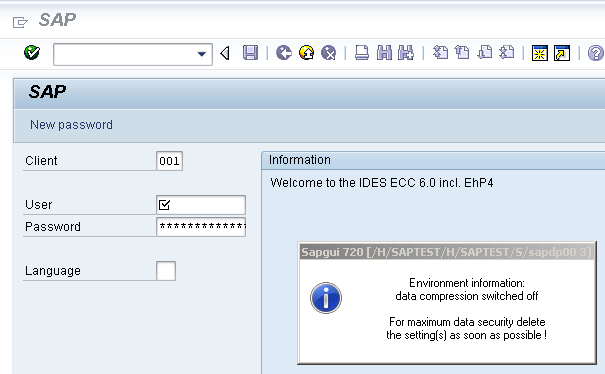
\includegraphics[scale=\FigScale]{examples/SAP/sapgui/sapgui720.png}
\caption{Screenshot}
\end{figure}

Let's see if we can remove the window somehow.

But before this, let's see what we already know.

First: we know that the environment variable \IT{\TDWNC} is checked somewhere inside the SAPGUI client.

Second: a string like \q{data compression switched off} must be present somewhere in it.
\newcommand{\FNURLFAR}{\footnote{\url{http://go.yurichev.com/17347}}}

With the help of the FAR file manager\FNURLFAR we can found that both of these strings are stored in the SAPguilib.dll file.

So let's open SAPguilib.dll in \IDA and search for the \IT{\q{\TDWNC}} string. 
Yes, it is present and there is only one reference to it.

We see the following fragment of code 
(all file offsets are valid for SAPGUI 720 win32, SAPguilib.dll file version 7200,1,0,9009):

\begin{lstlisting}
.text:6440D51B                 lea     eax, [ebp+2108h+var_211C]
.text:6440D51E                 push    eax             ; int
.text:6440D51F                 push    offset aTdw_nocompress ; "TDW_NOCOMPRESS"
.text:6440D524                 mov     byte ptr [edi+15h], 0
.text:6440D528                 call    chk_env
.text:6440D52D                 pop     ecx
.text:6440D52E                 pop     ecx
.text:6440D52F                 push    offset byte_64443AF8
.text:6440D534                 lea     ecx, [ebp+2108h+var_211C]

; demangled name: int ATL::CStringT::Compare(char const *)const
.text:6440D537                 call    ds:mfc90_1603
.text:6440D53D                 test    eax, eax
.text:6440D53F                 jz      short loc_6440D55A
.text:6440D541                 lea     ecx, [ebp+2108h+var_211C]

; demangled name: const char* ATL::CSimpleStringT::operator PCXSTR 
.text:6440D544                 call    ds:mfc90_910
.text:6440D54A                 push    eax             ; Str
.text:6440D54B                 call    ds:atoi
.text:6440D551                 test    eax, eax
.text:6440D553                 setnz   al
.text:6440D556                 pop     ecx
.text:6440D557                 mov     [edi+15h], al
\end{lstlisting}

\myindex{\CStandardLibrary!atoi()}

The string returned by \TT{chk\_env()} via its second argument is then handled by the MFC string functions and then 
\TT{atoi()}\footnote{standard C library function that converts the digits in a string to a number} is called. 
After that, the numerical value is stored in \TT{edi+15h}.

Also take a look at the \TT{chk\_env()} function (we gave this name to it manually):

\begin{lstlisting}
.text:64413F20 ; int __cdecl chk_env(char *VarName, int)
.text:64413F20 chk_env         proc near
.text:64413F20
.text:64413F20 DstSize         = dword ptr -0Ch
.text:64413F20 var_8           = dword ptr -8
.text:64413F20 DstBuf          = dword ptr -4
.text:64413F20 VarName         = dword ptr  8
.text:64413F20 arg_4           = dword ptr  0Ch
.text:64413F20
.text:64413F20                 push    ebp
.text:64413F21                 mov     ebp, esp
.text:64413F23                 sub     esp, 0Ch
.text:64413F26                 mov     [ebp+DstSize], 0
.text:64413F2D                 mov     [ebp+DstBuf], 0
.text:64413F34                 push    offset unk_6444C88C
.text:64413F39                 mov     ecx, [ebp+arg_4]

; (demangled name) ATL::CStringT::operator=(char const *)
.text:64413F3C                 call    ds:mfc90_820 
.text:64413F42                 mov     eax, [ebp+VarName]
.text:64413F45                 push    eax             ; VarName
.text:64413F46                 mov     ecx, [ebp+DstSize]
.text:64413F49                 push    ecx             ; DstSize
.text:64413F4A                 mov     edx, [ebp+DstBuf]
.text:64413F4D                 push    edx             ; DstBuf
.text:64413F4E                 lea     eax, [ebp+DstSize]
.text:64413F51                 push    eax             ; ReturnSize
.text:64413F52                 call    ds:getenv_s
.text:64413F58                 add     esp, 10h
.text:64413F5B                 mov     [ebp+var_8], eax
.text:64413F5E                 cmp     [ebp+var_8], 0
.text:64413F62                 jz      short loc_64413F68
.text:64413F64                 xor     eax, eax
.text:64413F66                 jmp     short loc_64413FBC
.text:64413F68
.text:64413F68 loc_64413F68:
.text:64413F68                 cmp     [ebp+DstSize], 0
.text:64413F6C                 jnz     short loc_64413F72
.text:64413F6E                 xor     eax, eax
.text:64413F70                 jmp     short loc_64413FBC
.text:64413F72
.text:64413F72 loc_64413F72:
.text:64413F72                 mov     ecx, [ebp+DstSize]
.text:64413F75                 push    ecx
.text:64413F76                 mov     ecx, [ebp+arg_4]

; demangled name: ATL::CSimpleStringT<char, 1>::Preallocate(int)
.text:64413F79                 call    ds:mfc90_2691
.text:64413F7F                 mov     [ebp+DstBuf], eax
.text:64413F82                 mov     edx, [ebp+VarName]
.text:64413F85                 push    edx             ; VarName
.text:64413F86                 mov     eax, [ebp+DstSize]
.text:64413F89                 push    eax             ; DstSize
.text:64413F8A                 mov     ecx, [ebp+DstBuf]
.text:64413F8D                 push    ecx             ; DstBuf
.text:64413F8E                 lea     edx, [ebp+DstSize]
.text:64413F91                 push    edx             ; ReturnSize
.text:64413F92                 call    ds:getenv_s
.text:64413F98                 add     esp, 10h
.text:64413F9B                 mov     [ebp+var_8], eax
.text:64413F9E                 push    0FFFFFFFFh
.text:64413FA0                 mov     ecx, [ebp+arg_4]

; demangled name: ATL::CSimpleStringT::ReleaseBuffer(int)
.text:64413FA3                 call    ds:mfc90_5835
.text:64413FA9                 cmp     [ebp+var_8], 0
.text:64413FAD                 jz      short loc_64413FB3
.text:64413FAF                 xor     eax, eax
.text:64413FB1                 jmp     short loc_64413FBC
.text:64413FB3
.text:64413FB3 loc_64413FB3:
.text:64413FB3                 mov     ecx, [ebp+arg_4]

; demangled name: const char* ATL::CSimpleStringT::operator PCXSTR 
.text:64413FB6                 call    ds:mfc90_910
.text:64413FBC
.text:64413FBC loc_64413FBC:
.text:64413FBC
.text:64413FBC                 mov     esp, ebp
.text:64413FBE                 pop     ebp
.text:64413FBF                 retn
.text:64413FBF chk_env         endp
\end{lstlisting}

\myindex{\CStandardLibrary!getenv()}
Yes. The \TT{getenv\_s()}\footnote{\href{http://go.yurichev.com/17250}{MSDN}} 

function is a Microsoft security-enhanced version of \TT{getenv()}\footnote{Standard C library returning environment variable}.

\myindex{MFC}

There are also some MFC string manipulations.

Lots of other environment variables are checked as well. 
Here is a list of all variables that are being checked and what SAPGUI would write to its trace log when logging is turned on:

\begin{center}
\begin{tabular}{ | l | l | }
\hline                        
DPTRACE                  & ``GUI-OPTION: Trace set to \%d'' \\
TDW\_HEXDUMP             & ``GUI-OPTION: Hexdump enabled'' \\
TDW\_WORKDIR             & ``GUI-OPTION: working directory `\%s\''' \\
TDW\_SPLASHSRCEENOFF     & ``GUI-OPTION: Splash Screen Off'' / ``GUI-OPTION: Splash Screen On'' \\
TDW\_REPLYTIMEOUT        & ``GUI-OPTION: reply timeout \%d milliseconds'' \\
TDW\_PLAYBACKTIMEOUT     & ``GUI-OPTION: PlaybackTimeout  set to \%d milliseconds'' \\ 
TDW\_NOCOMPRESS          & ``GUI-OPTION: no compression read'' \\
TDW\_EXPERT              & ``GUI-OPTION: expert mode'' \\
TDW\_PLAYBACKPROGRESS    & ``GUI-OPTION: PlaybackProgress'' \\
TDW\_PLAYBACKNETTRAFFIC  & ``GUI-OPTION: PlaybackNetTraffic'' \\
TDW\_PLAYLOG             & ``GUI-OPTION: /PlayLog is YES, file \%s'' \\
TDW\_PLAYTIME            & ``GUI-OPTION: /PlayTime set to \%d milliseconds'' \\
TDW\_LOGFILE             & ``GUI-OPTION: TDW\_LOGFILE `\%s\''' \\
TDW\_WAN                 & ``GUI-OPTION: WAN - low speed connection enabled'' \\
TDW\_FULLMENU            & ``GUI-OPTION: FullMenu enabled'' \\
SAP\_CP / SAP\_CODEPAGE  & ``GUI-OPTION: SAP\_CODEPAGE `\%d\''' \\
UPDOWNLOAD\_CP           & ``GUI-OPTION: UPDOWNLOAD\_CP `\%d\''' \\
SNC\_PARTNERNAME         & ``GUI-OPTION: SNC name `\%s\''' \\
SNC\_QOP                 & ``GUI-OPTION: SNC\_QOP `\%s\''' \\
SNC\_LIB                 & ``GUI-OPTION: SNC is set to: \%s'' \\ 
SAPGUI\_INPLACE          & ``GUI-OPTION: environment variable SAPGUI\_INPLACE is on'' \\
\hline  
\end{tabular}
\end{center}

The settings for each variable are written in the array via a pointer in the \EDI register.
\EDI is set before the function call:

\begin{lstlisting}
.text:6440EE00                 lea     edi, [ebp+2884h+var_2884] ; options here like +0x15...
.text:6440EE03                 lea     ecx, [esi+24h]
.text:6440EE06                 call    load_command_line
.text:6440EE0B                 mov     edi, eax
.text:6440EE0D                 xor     ebx, ebx
.text:6440EE0F                 cmp     edi, ebx
.text:6440EE11                 jz      short loc_6440EE42
.text:6440EE13                 push    edi
.text:6440EE14                 push    offset aSapguiStoppedA ; "Sapgui stopped after commandline interp"...
.text:6440EE19                 push    dword_644F93E8
.text:6440EE1F                 call    FEWTraceError
\end{lstlisting}

Now, can we find the \IT{\q{data record mode switched on}} string?

Yes, and the only reference is in
\par \TT{CDwsGui::PrepareInfoWindow()}.

How do we get know the class/method names? There are a lot of special debugging calls that write to the log files, like:

\begin{lstlisting}
.text:64405160                 push    dword ptr [esi+2854h]
.text:64405166                 push    offset aCdwsguiPrepare ; "\nCDwsGui::PrepareInfoWindow: sapgui env"...
.text:6440516B                 push    dword ptr [esi+2848h]
.text:64405171                 call    dbg
.text:64405176                 add     esp, 0Ch
\end{lstlisting}

\dots or:

\begin{lstlisting}
.text:6440237A                 push    eax
.text:6440237B                 push    offset aCclientStart_6 ; "CClient::Start: set shortcut user to '\%"...
.text:64402380                 push    dword ptr [edi+4]
.text:64402383                 call    dbg
.text:64402388                 add     esp, 0Ch
\end{lstlisting}

It is \IT{very} useful.

So let's see the contents of this pesky annoying pop-up window's function:

\begin{lstlisting}
.text:64404F4F CDwsGui__PrepareInfoWindow proc near
.text:64404F4F
.text:64404F4F pvParam         = byte ptr -3Ch
.text:64404F4F var_38          = dword ptr -38h
.text:64404F4F var_34          = dword ptr -34h
.text:64404F4F rc              = tagRECT ptr -2Ch
.text:64404F4F cy              = dword ptr -1Ch
.text:64404F4F h               = dword ptr -18h
.text:64404F4F var_14          = dword ptr -14h
.text:64404F4F var_10          = dword ptr -10h
.text:64404F4F var_4           = dword ptr -4
.text:64404F4F
.text:64404F4F                 push    30h
.text:64404F51                 mov     eax, offset loc_64438E00
.text:64404F56                 call    __EH_prolog3
.text:64404F5B                 mov     esi, ecx        ; ECX is pointer to object
.text:64404F5D                 xor     ebx, ebx
.text:64404F5F                 lea     ecx, [ebp+var_14]
.text:64404F62                 mov     [ebp+var_10], ebx

; demangled name: ATL::CStringT(void)
.text:64404F65                 call    ds:mfc90_316    
.text:64404F6B                 mov     [ebp+var_4], ebx
.text:64404F6E                 lea     edi, [esi+2854h]
.text:64404F74                 push    offset aEnvironmentInf ; "Environment information:\n"
.text:64404F79                 mov     ecx, edi

; demangled name: ATL::CStringT::operator=(char const *)
.text:64404F7B                 call    ds:mfc90_820
.text:64404F81                 cmp     [esi+38h], ebx
.text:64404F84                 mov     ebx, ds:mfc90_2539
.text:64404F8A                 jbe     short loc_64404FA9
.text:64404F8C                 push    dword ptr [esi+34h]
.text:64404F8F                 lea     eax, [ebp+var_14]
.text:64404F92                 push    offset aWorkingDirecto ; "working directory: '\%s'\n"
.text:64404F97                 push    eax

; demangled name: ATL::CStringT::Format(char const *,...)
.text:64404F98                 call    ebx ; mfc90_2539
.text:64404F9A                 add     esp, 0Ch
.text:64404F9D                 lea     eax, [ebp+var_14]
.text:64404FA0                 push    eax
.text:64404FA1                 mov     ecx, edi

; demangled name: ATL::CStringT::operator+=(class ATL::CSimpleStringT<char, 1> const &)
.text:64404FA3                 call    ds:mfc90_941
.text:64404FA9
.text:64404FA9 loc_64404FA9:
.text:64404FA9                 mov     eax, [esi+38h]
.text:64404FAC                 test    eax, eax
.text:64404FAE                 jbe     short loc_64404FD3
.text:64404FB0                 push    eax
.text:64404FB1                 lea     eax, [ebp+var_14]
.text:64404FB4                 push    offset aTraceLevelDAct ; "trace level \%d activated\n"
.text:64404FB9                 push    eax

; demangled name: ATL::CStringT::Format(char const *,...)
.text:64404FBA                 call    ebx ; mfc90_2539
.text:64404FBC                 add     esp, 0Ch
.text:64404FBF                 lea     eax, [ebp+var_14]
.text:64404FC2                 push    eax
.text:64404FC3                 mov     ecx, edi

; demangled name: ATL::CStringT::operator+=(class ATL::CSimpleStringT<char, 1> const &)
.text:64404FC5                 call    ds:mfc90_941
.text:64404FCB                 xor     ebx, ebx
.text:64404FCD                 inc     ebx
.text:64404FCE                 mov     [ebp+var_10], ebx
.text:64404FD1                 jmp     short loc_64404FD6
.text:64404FD3
.text:64404FD3 loc_64404FD3:
.text:64404FD3                 xor     ebx, ebx
.text:64404FD5                 inc     ebx
.text:64404FD6
.text:64404FD6 loc_64404FD6:
.text:64404FD6                 cmp     [esi+38h], ebx
.text:64404FD9                 jbe     short loc_64404FF1
.text:64404FDB                 cmp     dword ptr [esi+2978h], 0
.text:64404FE2                 jz      short loc_64404FF1
.text:64404FE4                 push    offset aHexdumpInTrace ; "hexdump in trace activated\n"
.text:64404FE9                 mov     ecx, edi

; demangled name: ATL::CStringT::operator+=(char const *)
.text:64404FEB                 call    ds:mfc90_945
.text:64404FF1
.text:64404FF1 loc_64404FF1:
.text:64404FF1
.text:64404FF1                 cmp     byte ptr [esi+78h], 0
.text:64404FF5                 jz      short loc_64405007
.text:64404FF7                 push    offset aLoggingActivat ; "logging activated\n"
.text:64404FFC                 mov     ecx, edi

; demangled name: ATL::CStringT::operator+=(char const *)
.text:64404FFE                 call    ds:mfc90_945
.text:64405004                 mov     [ebp+var_10], ebx
.text:64405007
.text:64405007 loc_64405007:
.text:64405007                 cmp     byte ptr [esi+3Dh], 0
.text:6440500B                 jz      short bypass
.text:6440500D                 push    offset aDataCompressio ; "data compression switched off\n"
.text:64405012                 mov     ecx, edi

; demangled name: ATL::CStringT::operator+=(char const *)
.text:64405014                 call    ds:mfc90_945
.text:6440501A                 mov     [ebp+var_10], ebx
.text:6440501D
.text:6440501D bypass:
.text:6440501D                 mov     eax, [esi+20h]
.text:64405020                 test    eax, eax
.text:64405022                 jz      short loc_6440503A
.text:64405024                 cmp     dword ptr [eax+28h], 0
.text:64405028                 jz      short loc_6440503A
.text:6440502A                 push    offset aDataRecordMode ; "data record mode switched on\n"
.text:6440502F                 mov     ecx, edi

; demangled name: ATL::CStringT::operator+=(char const *)
.text:64405031                 call    ds:mfc90_945
.text:64405037                 mov     [ebp+var_10], ebx
.text:6440503A
.text:6440503A loc_6440503A:
.text:6440503A
.text:6440503A                 mov     ecx, edi
.text:6440503C                 cmp     [ebp+var_10], ebx
.text:6440503F                 jnz     loc_64405142
.text:64405045                 push    offset aForMaximumData ; "\nFor maximum data security delete\nthe s"...

; demangled name: ATL::CStringT::operator+=(char const *)
.text:6440504A                 call    ds:mfc90_945
.text:64405050                 xor     edi, edi
.text:64405052                 push    edi             ; fWinIni
.text:64405053                 lea     eax, [ebp+pvParam]
.text:64405056                 push    eax             ; pvParam
.text:64405057                 push    edi             ; uiParam
.text:64405058                 push    30h             ; uiAction
.text:6440505A                 call    ds:SystemParametersInfoA
.text:64405060                 mov     eax, [ebp+var_34]
.text:64405063                 cmp     eax, 1600
.text:64405068                 jle     short loc_64405072
.text:6440506A                 cdq
.text:6440506B                 sub     eax, edx
.text:6440506D                 sar     eax, 1
.text:6440506F                 mov     [ebp+var_34], eax
.text:64405072
.text:64405072 loc_64405072:
.text:64405072                 push    edi             ; hWnd
.text:64405073                 mov     [ebp+cy], 0A0h
.text:6440507A                 call    ds:GetDC
.text:64405080                 mov     [ebp+var_10], eax
.text:64405083                 mov     ebx, 12Ch
.text:64405088                 cmp     eax, edi
.text:6440508A                 jz      loc_64405113
.text:64405090                 push    11h             ; i
.text:64405092                 call    ds:GetStockObject
.text:64405098                 mov     edi, ds:SelectObject
.text:6440509E                 push    eax             ; h
.text:6440509F                 push    [ebp+var_10]    ; hdc
.text:644050A2                 call    edi ; SelectObject
.text:644050A4                 and     [ebp+rc.left], 0
.text:644050A8                 and     [ebp+rc.top], 0
.text:644050AC                 mov     [ebp+h], eax
.text:644050AF                 push    401h            ; format
.text:644050B4                 lea     eax, [ebp+rc]
.text:644050B7                 push    eax             ; lprc
.text:644050B8                 lea     ecx, [esi+2854h]
.text:644050BE                 mov     [ebp+rc.right], ebx
.text:644050C1                 mov     [ebp+rc.bottom], 0B4h

; demangled name: ATL::CSimpleStringT::GetLength(void)
.text:644050C8                 call    ds:mfc90_3178
.text:644050CE                 push    eax             ; cchText
.text:644050CF                 lea     ecx, [esi+2854h]

; demangled name: const char* ATL::CSimpleStringT::operator PCXSTR 
.text:644050D5                 call    ds:mfc90_910
.text:644050DB                 push    eax             ; lpchText
.text:644050DC                 push    [ebp+var_10]    ; hdc
.text:644050DF                 call    ds:DrawTextA
.text:644050E5                 push    4               ; nIndex
.text:644050E7                 call    ds:GetSystemMetrics
.text:644050ED                 mov     ecx, [ebp+rc.bottom]
.text:644050F0                 sub     ecx, [ebp+rc.top]
.text:644050F3                 cmp     [ebp+h], 0
.text:644050F7                 lea     eax, [eax+ecx+28h]
.text:644050FB                 mov     [ebp+cy], eax
.text:644050FE                 jz      short loc_64405108
.text:64405100                 push    [ebp+h]         ; h
.text:64405103                 push    [ebp+var_10]    ; hdc
.text:64405106                 call    edi ; SelectObject
.text:64405108
.text:64405108 loc_64405108:
.text:64405108                 push    [ebp+var_10]    ; hDC
.text:6440510B                 push    0               ; hWnd
.text:6440510D                 call    ds:ReleaseDC
.text:64405113
.text:64405113 loc_64405113:
.text:64405113                 mov     eax, [ebp+var_38]
.text:64405116                 push    80h             ; uFlags
.text:6440511B                 push    [ebp+cy]        ; cy
.text:6440511E                 inc     eax
.text:6440511F                 push    ebx             ; cx
.text:64405120                 push    eax             ; Y
.text:64405121                 mov     eax, [ebp+var_34]
.text:64405124                 add     eax, 0FFFFFED4h
.text:64405129                 cdq
.text:6440512A                 sub     eax, edx
.text:6440512C                 sar     eax, 1
.text:6440512E                 push    eax             ; X
.text:6440512F                 push    0               ; hWndInsertAfter
.text:64405131                 push    dword ptr [esi+285Ch] ; hWnd
.text:64405137                 call    ds:SetWindowPos
.text:6440513D                 xor     ebx, ebx
.text:6440513F                 inc     ebx
.text:64405140                 jmp     short loc_6440514D
.text:64405142
.text:64405142 loc_64405142:
.text:64405142                 push    offset byte_64443AF8

; demangled name: ATL::CStringT::operator=(char const *)
.text:64405147                 call    ds:mfc90_820
.text:6440514D
.text:6440514D loc_6440514D:
.text:6440514D                 cmp     dword_6450B970, ebx
.text:64405153                 jl      short loc_64405188
.text:64405155                 call    sub_6441C910
.text:6440515A                 mov     dword_644F858C, ebx
.text:64405160                 push    dword ptr [esi+2854h]
.text:64405166                 push    offset aCdwsguiPrepare ; "\nCDwsGui::PrepareInfoWindow: sapgui env"...
.text:6440516B                 push    dword ptr [esi+2848h]
.text:64405171                 call    dbg
.text:64405176                 add     esp, 0Ch
.text:64405179                 mov     dword_644F858C, 2
.text:64405183                 call    sub_6441C920
.text:64405188
.text:64405188 loc_64405188:
.text:64405188                 or      [ebp+var_4], 0FFFFFFFFh
.text:6440518C                 lea     ecx, [ebp+var_14]

; demangled name: ATL::CStringT::~CStringT()
.text:6440518F                 call    ds:mfc90_601
.text:64405195                 call    __EH_epilog3
.text:6440519A                 retn
.text:6440519A CDwsGui__PrepareInfoWindow endp
\end{lstlisting}

At the start of the function \ECX contains a pointer to the object (since it is a thiscall~(\myref{thiscall})-type of function).
In our case, the object obviously has class type of \IT{CDwsGui}. 
Depending on the option turned on in the object, a specific message part is to be concatenated with the resulting message.

If the value at address \TT{this+0x3D} is not zero, the compression is off:

\begin{lstlisting}
.text:64405007 loc_64405007:
.text:64405007                 cmp     byte ptr [esi+3Dh], 0
.text:6440500B                 jz      short bypass
.text:6440500D                 push    offset aDataCompressio ; "data compression switched off\n"
.text:64405012                 mov     ecx, edi

; demangled name: ATL::CStringT::operator+=(char const *)
.text:64405014                 call    ds:mfc90_945
.text:6440501A                 mov     [ebp+var_10], ebx
.text:6440501D
.text:6440501D bypass:
\end{lstlisting}

It is interesting that finally the \IT{var\_10} variable state defines whether the message is to be shown at all:

\lstinputlisting{examples/SAP/sapgui/1_EN}

Let's check our theory on practice.

\JNZ at this line \dots

\lstinputlisting{examples/SAP/sapgui/2_EN}

\dots 
replace it with just \JMP, and we get SAPGUI working without the pesky annoying pop-up window appearing!

Now let's dig deeper and find a connection between the $0x15$ offset in the \TT{load\_command\_line()} 
(we gave it this name) function and the \TT{this+0x3D} variable in \IT{CDwsGui::PrepareInfoWindow}. 
Are we sure the value is the same?

We are starting to search for all occurrences of the \TT{0x15} value in code. 
For a small programs like SAPGUI, it sometimes works. Here is the first occurrence we've got:

\begin{lstlisting}
.text:64404C19 sub_64404C19    proc near
.text:64404C19
.text:64404C19 arg_0           = dword ptr  4
.text:64404C19
.text:64404C19                 push    ebx
.text:64404C1A                 push    ebp
.text:64404C1B                 push    esi
.text:64404C1C                 push    edi
.text:64404C1D                 mov     edi, [esp+10h+arg_0]
.text:64404C21                 mov     eax, [edi]
.text:64404C23                 mov     esi, ecx ; ESI/ECX are pointers to some unknown object.
.text:64404C25                 mov     [esi], eax
.text:64404C27                 mov     eax, [edi+4]
.text:64404C2A                 mov     [esi+4], eax
.text:64404C2D                 mov     eax, [edi+8]
.text:64404C30                 mov     [esi+8], eax
.text:64404C33                 lea     eax, [edi+0Ch]
.text:64404C36                 push    eax
.text:64404C37                 lea     ecx, [esi+0Ch]

; demangled name:  ATL::CStringT::operator=(class ATL::CStringT ... &)
.text:64404C3A                 call    ds:mfc90_817 
.text:64404C40                 mov     eax, [edi+10h]
.text:64404C43                 mov     [esi+10h], eax
.text:64404C46                 mov     al, [edi+14h]
.text:64404C49                 mov     [esi+14h], al
.text:64404C4C                 mov     al, [edi+15h] ; copy byte from 0x15 offset
.text:64404C4F                 mov     [esi+15h], al ; to 0x15 offset in CDwsGui object
\end{lstlisting}

The function was called from the function named \IT{CDwsGui::CopyOptions}! And thanks again for debugging information.

But the real answer is in \IT{CDwsGui::Init()}:

\begin{lstlisting}
.text:6440B0BF loc_6440B0BF:
.text:6440B0BF                 mov     eax, [ebp+arg_0]
.text:6440B0C2                 push    [ebp+arg_4]
.text:6440B0C5                 mov     [esi+2844h], eax
.text:6440B0CB                 lea     eax, [esi+28h] ; ESI is pointer to CDwsGui object
.text:6440B0CE                 push    eax
.text:6440B0CF                 call    CDwsGui__CopyOptions
\end{lstlisting}

Finally, we understand: the array filled in the \TT{load\_command\_line()} function is actually placed in the \IT{CDwsGui} class, 
but at address \TT{this+0x28}. 0x15 + 0x28 is exactly 0x3D. OK, we found the point where the value is copied to.

Let's also find the rest of the places where the 0x3D offset is used. 
Here is one of them in the \IT{CDwsGui::SapguiRun} function (again, thanks to the debugging calls):

\begin{lstlisting}
.text:64409D58                 cmp     [esi+3Dh], bl   ; ESI is pointer to CDwsGui object
.text:64409D5B                 lea     ecx, [esi+2B8h]
.text:64409D61                 setz    al
.text:64409D64                 push    eax             ; arg_10 of CConnectionContext::CreateNetwork
.text:64409D65                 push    dword ptr [esi+64h]

; demangled name: const char* ATL::CSimpleStringT::operator PCXSTR 
.text:64409D68                 call    ds:mfc90_910
.text:64409D68                                         ; no arguments
.text:64409D6E                 push    eax
.text:64409D6F                 lea     ecx, [esi+2BCh]

; demangled name: const char* ATL::CSimpleStringT::operator PCXSTR 
.text:64409D75                 call    ds:mfc90_910
.text:64409D75                                         ; no arguments
.text:64409D7B                 push    eax
.text:64409D7C                 push    esi
.text:64409D7D                 lea     ecx, [esi+8]
.text:64409D80                 call    CConnectionContext__CreateNetwork
\end{lstlisting}

Let's check our findings. Replace the \TT{setz al} here with the \TT{xor eax, eax / nop} instructions,
clear the \TDWNC 
environment variable and run SAPGUI. Wow! There pesky annoying window is no more (just as expected, 
because the variable is not set) but in Wireshark we can see that the network packets are not compressed anymore! 
Obviously, this is the point where the compression flag is to be set in the \IT{CConnectionContext} object.

So, the compression flag is passed in the 5th argument of \IT{CConnectionContext::CreateNetwork}. 
Inside the function, another one is called:

\begin{lstlisting}
...
.text:64403476                 push    [ebp+compression]
.text:64403479                 push    [ebp+arg_C]
.text:6440347C                 push    [ebp+arg_8]
.text:6440347F                 push    [ebp+arg_4]
.text:64403482                 push    [ebp+arg_0]
.text:64403485                 call    CNetwork__CNetwork
\end{lstlisting}

The compression flag is passed here in the 5th argument to the \IT{CNetwork::CNetwork} constructor.

And here is how the \IT{CNetwork} constructor sets the flag in the \IT{CNetwork} object according to its 5th argument \IT{and}
another variable which probably could also affect network packets compression.

\begin{lstlisting}
.text:64411DF1                 cmp     [ebp+compression], esi
.text:64411DF7                 jz      short set_EAX_to_0
.text:64411DF9                 mov     al, [ebx+78h]   ; another value may affect compression?
.text:64411DFC                 cmp     al, '3'
.text:64411DFE                 jz      short set_EAX_to_1
.text:64411E00                 cmp     al, '4'
.text:64411E02                 jnz     short set_EAX_to_0
.text:64411E04
.text:64411E04 set_EAX_to_1:
.text:64411E04                 xor     eax, eax
.text:64411E06                 inc     eax             ; EAX -> 1
.text:64411E07                 jmp     short loc_64411E0B
.text:64411E09
.text:64411E09 set_EAX_to_0:
.text:64411E09
.text:64411E09                 xor     eax, eax        ; EAX -> 0
.text:64411E0B
.text:64411E0B loc_64411E0B:
.text:64411E0B                 mov     [ebx+3A4h], eax ; EBX is pointer to CNetwork object
\end{lstlisting}

At this point we know the compression flag is stored in the \IT{CNetwork} class at address \IT{this+0x3A4}.

Now let's dig through SAPguilib.dll for the \TT{0x3A4} value. And here is the second occurrence in 
\IT{CDwsGui::OnClientMessageWrite} (endless thanks for the debugging information):

\begin{lstlisting}
.text:64406F76 loc_64406F76:
.text:64406F76                 mov     ecx, [ebp+7728h+var_7794]
.text:64406F79                 cmp     dword ptr [ecx+3A4h], 1
.text:64406F80                 jnz     compression_flag_is_zero
.text:64406F86                 mov     byte ptr [ebx+7], 1
.text:64406F8A                 mov     eax, [esi+18h]
.text:64406F8D                 mov     ecx, eax
.text:64406F8F                 test    eax, eax
.text:64406F91                 ja      short loc_64406FFF
.text:64406F93                 mov     ecx, [esi+14h]
.text:64406F96                 mov     eax, [esi+20h]
.text:64406F99
.text:64406F99 loc_64406F99:
.text:64406F99                 push    dword ptr [edi+2868h] ; int
.text:64406F9F                 lea     edx, [ebp+7728h+var_77A4]
.text:64406FA2                 push    edx             ; int
.text:64406FA3                 push    30000           ; int
.text:64406FA8                 lea     edx, [ebp+7728h+Dst]
.text:64406FAB                 push    edx             ; Dst
.text:64406FAC                 push    ecx             ; int
.text:64406FAD                 push    eax             ; Src
.text:64406FAE                 push    dword ptr [edi+28C0h] ; int
.text:64406FB4                 call    sub_644055C5       ; actual compression routine
.text:64406FB9                 add     esp, 1Ch
.text:64406FBC                 cmp     eax, 0FFFFFFF6h
.text:64406FBF                 jz      short loc_64407004
.text:64406FC1                 cmp     eax, 1
.text:64406FC4                 jz      loc_6440708C
.text:64406FCA                 cmp     eax, 2
.text:64406FCD                 jz      short loc_64407004
.text:64406FCF                 push    eax
.text:64406FD0                 push    offset aCompressionErr ; "compression error [rc = \%d]- program wi"...
.text:64406FD5                 push    offset aGui_err_compre ; "GUI_ERR_COMPRESS"
.text:64406FDA                 push    dword ptr [edi+28D0h]
.text:64406FE0                 call    SapPcTxtRead
\end{lstlisting}

Let's take a look in \IT{sub\_644055C5}. In it we can only see the call to memcpy() and another function named 
(by \IDA) \IT{sub\_64417440}.

And, let's take a look inside \IT{sub\_64417440}. What we see is:

\begin{lstlisting}
.text:6441747C                 push    offset aErrorCsrcompre ; "\nERROR: CsRCompress: invalid handle"
.text:64417481                 call    eax ; dword_644F94C8
.text:64417483                 add     esp, 4
\end{lstlisting}

Voilà! We've found the function that actually compresses the data.
As it was shown in past
\footnote{\url{http://go.yurichev.com/17312}},

this function is used in SAP and also the open-source MaxDB project. 
So it is available in source form.

Doing the last check here:

\begin{lstlisting}
.text:64406F79                 cmp     dword ptr [ecx+3A4h], 1
.text:64406F80                 jnz     compression_flag_is_zero
\end{lstlisting}

Replace \JNZ here for an unconditional \JMP. Remove the environment variable \TDWNC. Voilà!

In Wireshark we see that the client messages are not compressed. The server responses, however, are compressed.

So we found exact connection between the environment variable and the point where data compression 
routine can be called or bypassed.

}
\section{\RU{Функции проверки пароля в SAP 6.0}\EN{SAP 6.0 password checking functions}}

\index{SAP}
\RU{Когда я в очередной раз вернулся к своему SAP 6.0 IDES заинсталлированному в виртуальной машине VMware, я обнаружил что забыл пароль, впрочем, затем я вспомнил его, но теперь я получаю такую ошибку:}\EN{One time when I returned again to my SAP 6.0 IDES installed in a VMware box, I figured out that I forgot the password for the SAP* account, then I remembered it, but then I got this error message} 
\IT{<<Password logon no longer possible - too many failed attempts>>}, 
\RU{потому что я потратил все попытки на то, чтобы вспомнить его}
\EN{since I've made all these attempts in trying to recall it}.

\index{Windows!PDB}
\RU{Первая очень хорошая новость состоит в том, что с SAP поставляется полный \gls{PDB}-файл \IT{disp+work.pdb}, он содержит все: имена функций, структуры, типы, локальные переменные, имена аргументов, \etc{}. Какой щедрый подарок!}
\EN{The first extremely good news was that the full \IT{disp+work.pdb} \gls{PDB} file is supplied with SAP, and it contain almost everything: function names, structures, types, local variable and argument names, \etc{}. What a lavish gift!}

\RU{Я нашел утилиту}\EN{I found the} TYPEINFODUMP\footnote{\url{http://go.yurichev.com/17038}} \RU{для дампа содержимого \gls{PDB}-файлов во что-то более читаемое и grep-абельное}\EN{utility for converting \gls{PDB} files into something readable and grepable}.

\RU{Вот пример её работы: информация о функции + её аргументах + её локальных переменных:}\EN{Here is an example of a function information + its arguments + its local variables:}

\begin{lstlisting}
FUNCTION ThVmcSysEvent 
  Address:         10143190  Size:      675 bytes  Index:    60483  TypeIndex:    60484 
  Type: int NEAR_C ThVmcSysEvent (unsigned int, unsigned char, unsigned short*)
Flags: 0 
PARAMETER events 
  Address: Reg335+288  Size:        4 bytes  Index:    60488  TypeIndex:    60489 
  Type: unsigned int
Flags: d0 
PARAMETER opcode 
  Address: Reg335+296  Size:        1 bytes  Index:    60490  TypeIndex:    60491 
  Type: unsigned char
Flags: d0 
PARAMETER serverName 
  Address: Reg335+304  Size:        8 bytes  Index:    60492  TypeIndex:    60493 
  Type: unsigned short*
Flags: d0 
STATIC_LOCAL_VAR func 
  Address:         12274af0  Size:        8 bytes  Index:    60495  TypeIndex:    60496 
  Type: wchar_t*
Flags: 80 
LOCAL_VAR admhead 
  Address: Reg335+304  Size:        8 bytes  Index:    60498  TypeIndex:    60499 
  Type: unsigned char*
Flags: 90 
LOCAL_VAR record 
  Address: Reg335+64  Size:      204 bytes  Index:    60501  TypeIndex:    60502 
  Type: AD_RECORD
Flags: 90 
LOCAL_VAR adlen 
  Address: Reg335+296  Size:        4 bytes  Index:    60508  TypeIndex:    60509 
  Type: int
Flags: 90 
\end{lstlisting}

\RU{А вот пример дампа структуры:}\EN{And here is an example of some structure:}

\begin{lstlisting}
STRUCT DBSL_STMTID 
Size: 120  Variables: 4  Functions: 0  Base classes: 0
MEMBER moduletype 
  Type:  DBSL_MODULETYPE
  Offset:        0  Index:        3  TypeIndex:    38653
MEMBER module 
  Type:  wchar_t module[40]
  Offset:        4  Index:        3  TypeIndex:      831
MEMBER stmtnum 
  Type:  long
  Offset:       84  Index:        3  TypeIndex:      440
MEMBER timestamp 
  Type:  wchar_t timestamp[15]
  Offset:       88  Index:        3  TypeIndex:     6612
\end{lstlisting}

\RU{Вау!}\EN{Wow!}

\RU{Вторая хорошая новость: \IT{отладочные} вызовы, коих здесь очень много, очень полезны.}\EN{Another good news: \IT{debugging} calls (there are plenty of them) are very useful.} 

\RU{Здесь вы можете увидеть глобальную переменную \IT{ct\_level}}\EN{Here you can also notice the \IT{ct\_level} global variable}\footnote{\RU{Еще об уровне трассировки}\EN{More about trace level}: \url{http://go.yurichev.com/17039}}, \RU{отражающую уровень трассировки}\EN{that reflects the current trace level}.

\RU{В \IT{disp+work.exe} очень много таких отладочных вставок}\EN{There are a lot of debugging inserts in the \IT{disp+work.exe} file}:

\begin{lstlisting}
cmp     cs:ct_level, 1
jl      short loc_1400375DA
call    DpLock
lea     rcx, aDpxxtool4_c ; "dpxxtool4.c"
mov     edx, 4Eh        ; line
call    CTrcSaveLocation
mov     r8, cs:func_48
mov     rcx, cs:hdl     ; hdl
lea     rdx, aSDpreadmemvalu ; "%s: DpReadMemValue (%d)"
mov     r9d, ebx
call    DpTrcErr
call    DpUnlock
\end{lstlisting}

\RU{Если текущий уровень трассировки выше или равен заданному в этом коде порогу, 
отладочное сообщение будет записано в лог-файл вроде \IT{dev\_w0}, \IT{dev\_disp} 
и прочие файлы \IT{dev*}.}
\EN{If the current trace level is bigger or equal to threshold defined in the code here, 
a debugging message is to be written to the log files like \IT{dev\_w0}, \IT{dev\_disp}, 
and other \IT{dev*} files.}

\index{\GrepUsage}
\RU{Попробуем grep-ать файл полученный при помощи утилиты TYPEINFODUMP:}\EN{Let's try grepping in the file that I got with the help of the TYPEINFODUMP utility:}

\begin{lstlisting}
cat "disp+work.pdb.d" | grep FUNCTION | grep -i password
\end{lstlisting}

\RU{Я получил:}\EN{I got:}

\begin{lstlisting}
FUNCTION rcui::AgiPassword::DiagISelection 
FUNCTION ssf_password_encrypt 
FUNCTION ssf_password_decrypt 
FUNCTION password_logon_disabled 
FUNCTION dySignSkipUserPassword 
FUNCTION migrate_password_history 
FUNCTION password_is_initial 
FUNCTION rcui::AgiPassword::IsVisible 
FUNCTION password_distance_ok 
FUNCTION get_password_downwards_compatibility 
FUNCTION dySignUnSkipUserPassword 
FUNCTION rcui::AgiPassword::GetTypeName 
FUNCTION `rcui::AgiPassword::AgiPassword'::`1'::dtor$2 
FUNCTION `rcui::AgiPassword::AgiPassword'::`1'::dtor$0 
FUNCTION `rcui::AgiPassword::AgiPassword'::`1'::dtor$1 
FUNCTION usm_set_password 
FUNCTION rcui::AgiPassword::TraceTo 
FUNCTION days_since_last_password_change 
FUNCTION rsecgrp_generate_random_password 
FUNCTION rcui::AgiPassword::`scalar deleting destructor' 
FUNCTION password_attempt_limit_exceeded 
FUNCTION handle_incorrect_password 
FUNCTION `rcui::AgiPassword::`scalar deleting destructor''::`1'::dtor$1 
FUNCTION calculate_new_password_hash 
FUNCTION shift_password_to_history 
FUNCTION rcui::AgiPassword::GetType 
FUNCTION found_password_in_history 
FUNCTION `rcui::AgiPassword::`scalar deleting destructor''::`1'::dtor$0 
FUNCTION rcui::AgiObj::IsaPassword 
FUNCTION password_idle_check 
FUNCTION SlicHwPasswordForDay 
FUNCTION rcui::AgiPassword::IsaPassword 
FUNCTION rcui::AgiPassword::AgiPassword 
FUNCTION delete_user_password 
FUNCTION usm_set_user_password 
FUNCTION Password_API 
FUNCTION get_password_change_for_SSO 
FUNCTION password_in_USR40 
FUNCTION rsec_agrp_abap_generate_random_password 
\end{lstlisting}

\RU{Попробуем так же искать отладочные сообщения содержащие слова \IT{<<password>>} и \IT{<<locked>>}.}\EN{Let's also try to search for debug messages which contain the words \IT{<<password>>} and \IT{<<locked>>}.}
\RU{Одна из таких это строка}\EN{One of them is the string} \IT{<<user was locked by subsequently failed password logon attempts>>} \RU{на которую есть ссылка в}\EN{, referenced in} \\
\RU{функции}\EN{function} \IT{password\_attempt\_limit\_exceeded()}.

\RU{Другие строки, которые эта найденная функция может писать в лог-файл это}
\EN{Other strings that this function can write to a log file are}: 
\IT{<<password logon attempt will be rejected immediately (preventing dictionary attacks)>>}, \IT{<<failed-logon lock: expired (but not removed due to 'read-only' operation)>>}, \IT{<<failed-logon lock: expired => removed>>}.

\RU{Немного поэкспериментировав с этой функцией, я быстро понял что проблема именно в ней}\EN{After playing for a little with this function, I noticed that the problem is exactly in it}. \RU{Она вызывается из функции \IT{chckpass()}\EMDASH{}одна из функций проверяющих пароль}\EN{It is called from the \IT{chckpass()} function~---one of the password checking functions}.

\RU{В начале, я хочу убедиться, что я на верном пути}\EN{First, I would like to make sure that I'm at the correct point}:

\RU{Запускаю свой}\EN{Run my} \tracer:
\index{tracer}

\begin{lstlisting}
tracer64.exe -a:disp+work.exe bpf=disp+work.exe!chckpass,args:3,unicode
\end{lstlisting}

\begin{lstlisting}
PID=2236|TID=2248|(0) disp+work.exe!chckpass (0x202c770, L"Brewered1                               ", 0x41) (called from 0x1402f1060 (disp+work.exe!usrexist+0x3c0))
PID=2236|TID=2248|(0) disp+work.exe!chckpass -> 0x35
\end{lstlisting}

\RU{Функции вызываются так}\EN{The call path is}: \IT{syssigni()} -> \IT{DyISigni()} -> \IT{dychkusr()} -> \IT{usrexist()} -> \IT{chckpass()}.

\RU{Число}\EN{The number} 0x35 \RU{возвращается из}\EN{is an error returned in} \IT{chckpass()} \RU{в этом месте}\EN{at that point}:

\begin{lstlisting}
.text:00000001402ED567 loc_1402ED567:                          ; CODE XREF: chckpass+B4
.text:00000001402ED567                 mov     rcx, rbx        ; usr02
.text:00000001402ED56A                 call    password_idle_check
.text:00000001402ED56F                 cmp     eax, 33h
.text:00000001402ED572                 jz      loc_1402EDB4E
.text:00000001402ED578                 cmp     eax, 36h
.text:00000001402ED57B                 jz      loc_1402EDB3D
.text:00000001402ED581                 xor     edx, edx        ; usr02_readonly
.text:00000001402ED583                 mov     rcx, rbx        ; usr02
.text:00000001402ED586                 call    password_attempt_limit_exceeded
.text:00000001402ED58B                 test    al, al
.text:00000001402ED58D                 jz      short loc_1402ED5A0
.text:00000001402ED58F                 mov     eax, 35h
.text:00000001402ED594                 add     rsp, 60h
.text:00000001402ED598                 pop     r14
.text:00000001402ED59A                 pop     r12
.text:00000001402ED59C                 pop     rdi
.text:00000001402ED59D                 pop     rsi
.text:00000001402ED59E                 pop     rbx
.text:00000001402ED59F                 retn
\end{lstlisting}

\RU{Отлично, давайте проверим}\EN{Fine, let's check}:

\begin{lstlisting}
tracer64.exe -a:disp+work.exe bpf=disp+work.exe!password_attempt_limit_exceeded,args:4,unicode,rt:0
\end{lstlisting}

\begin{lstlisting}
PID=2744|TID=360|(0) disp+work.exe!password_attempt_limit_exceeded (0x202c770, 0, 0x257758, 0) (called from 0x1402ed58b (disp+work.exe!chckpass+0xeb))
PID=2744|TID=360|(0) disp+work.exe!password_attempt_limit_exceeded -> 1
PID=2744|TID=360|We modify return value (EAX/RAX) of this function to 0
PID=2744|TID=360|(0) disp+work.exe!password_attempt_limit_exceeded (0x202c770, 0, 0, 0) (called from 0x1402e9794 (disp+work.exe!chngpass+0xe4))
PID=2744|TID=360|(0) disp+work.exe!password_attempt_limit_exceeded -> 1
PID=2744|TID=360|We modify return value (EAX/RAX) of this function to 0
\end{lstlisting}

\RU{Великолепно! Теперь я могу успешно залогиниться.}\EN{Excellent! I can successfully login now.}

\RU{Кстати, я могу сделать вид что вообще забыл пароль, заставляя \IT{chckpass()} всегда возвращать ноль, и этого достаточно для отключения проверки пароля:}
\EN{By the way, if I forgot the password, fixing the \IT{chckpass()} function to return a value of 0 is enough to bypass the check:}

\begin{lstlisting}
tracer64.exe -a:disp+work.exe bpf=disp+work.exe!chckpass,args:3,unicode,rt:0
\end{lstlisting}

\begin{lstlisting}
PID=2744|TID=360|(0) disp+work.exe!chckpass (0x202c770, L"bogus                                   ", 0x41) (called from 0x1402f1060 (disp+work.exe!usrexist+0x3c0))
PID=2744|TID=360|(0) disp+work.exe!chckpass -> 0x35
PID=2744|TID=360|We modify return value (EAX/RAX) of this function to 0
\end{lstlisting}

\RU{Что еще можно сказать, бегло анализируя функцию \IT{password\_attempt\_limit\_exceeded()}, это то, что в начале
можно увидеть следующий вызов:}\EN{What also can be said while analyzing the 
\IT{password\_attempt\_limit\_exceeded()} 
function is that at the very beginning of it, this call can be seen:}

\begin{lstlisting}
lea     rcx, aLoginFailed_us ; "login/failed_user_auto_unlock"
call    sapgparam
test    rax, rax
jz      short loc_1402E19DE
movzx   eax, word ptr [rax]
cmp     ax, 'N'
jz      short loc_1402E19D4
cmp     ax, 'n'
jz      short loc_1402E19D4
cmp     ax, '0'
jnz     short loc_1402E19DE
\end{lstlisting}

\RU{Очевидно, функция \IT{sapgparam()} используется чтобы узнать значение какой-либо переменной конфигурации. Эта функция может вызываться из 1768 разных мест.}
\EN{Obviously, function \IT{sapgparam()} is used to query the value of some configuration parameter. This function can be called from 1768 different places.}
\RU{Вероятно, при помощи этой информации, мы можем легко находить те места кода, на которые влияют определенные переменные конфигурации.}\EN{It seems that with the help of this information, we can easily find the places in code, the control flow of which can be affected by specific configuration parameters.}

\RU{Замечательно! Имена функций очень понятны, куда понятнее чем в \oracle.}
\EN{It is really sweet. The function names are very clear, much clearer than in the \oracle.} 
\index{\Cpp}
\RU{По всей видимости, процесс \IT{disp+work} весь написан на \Cpp. Вероятно, он был переписан не так давно?}
\EN{It seems that the \IT{disp+work} process is written in \Cpp. It was apparently rewritten some time ago?}



\chapter{\oracle}
\label{oracle}

% sections
\section{\EN{.SYM-files}\RU{.SYM-файлы}}

\RU{Когда процесс в \oracle терпит серьезную ошибку (crash), он записывает массу информации в лог-файлы,
включая состояние стека, вроде:}
\EN{When \oracle process experiencing some kind of crash, it writes a lot of information into log files,
including stack trace, like:}

\begin{lstlisting}
----- Call Stack Trace -----
calling              call     entry                argument values in hex      
location             type     point                (? means dubious value)     
-------------------- -------- -------------------- ----------------------------
_kqvrow()                     00000000             
_opifch2()+2729      CALLptr  00000000             23D4B914 E47F264 1F19AE2
                                                   EB1C8A8 1
_kpoal8()+2832       CALLrel  _opifch2()           89 5 EB1CC74
_opiodr()+1248       CALLreg  00000000             5E 1C EB1F0A0
_ttcpip()+1051       CALLreg  00000000             5E 1C EB1F0A0 0
_opitsk()+1404       CALL???  00000000             C96C040 5E EB1F0A0 0 EB1ED30
                                                   EB1F1CC 53E52E 0 EB1F1F8
_opiino()+980        CALLrel  _opitsk()            0 0
_opiodr()+1248       CALLreg  00000000             3C 4 EB1FBF4
_opidrv()+1201       CALLrel  _opiodr()            3C 4 EB1FBF4 0
_sou2o()+55          CALLrel  _opidrv()            3C 4 EB1FBF4
_opimai_real()+124   CALLrel  _sou2o()             EB1FC04 3C 4 EB1FBF4
_opimai()+125        CALLrel  _opimai_real()       2 EB1FC2C
_OracleThreadStart@  CALLrel  _opimai()            2 EB1FF6C 7C88A7F4 EB1FC34 0
4()+830                                            EB1FD04
77E6481C             CALLreg  00000000             E41FF9C 0 0 E41FF9C 0 EB1FFC4
00000000             CALL???  00000000             
\end{lstlisting}

\RU{Но конечно, для этого исполняемые файлы \oracle должны содержать некоторую отладочную информацию,
либо map-файлы с инфомрацией о символах или что-то в этом роде.}
\EN{But of course, \oracle executables must have some kind of debug information or map files with symbol
information included or something like that.}

\RU{\oracle для Windows NT содержит информацию о символах в файлах с расширением .SYM, но его формат закрыт.}
\EN{Windows NT \oracle have symbol information in files with .SYM extension, but the format is proprietary.}
\EN{(Plain text files are good, but needs additional parsing, hence offer slower access.)}
\RU{(Простые текстовые файлы это хорошо, но они требуют дополнительной обработки (парсинга), и из-за этого доступ
к ним медленнее.)}

\RU{Посмотрим, сможем ли мы разобрать его формат}\EN{Let's see if we can understand its format}.
\RU{Я выбрал самый короткий файл \TT{orawtc8.sym}, поставляемый с файлом \TT{orawtc8.dll} в Oracle 8.1.7}
\EN{I chose shortest \TT{orawtc8.sym} file, coming with \TT{orawtc8.dll} file in Oracle 8.1.7}
\footnote{\RU{Я выбрал древнюю версию \oracle сознательно, из-за более короткого размера его модулей}\EN{I chose 
ancient \oracle version intentionally due to smaller size of its modules}}.

\RU{Вот я открываю этот файл в}\EN{Here is the file opened in} Hiew: \figref{fig:oracle_SYM_whole1}.

\RU{Сравнивая этот файл с другими .SYM-файлами, мы можем быстро заметить что \TT{OSYM} всегда является
заголовком (и концом), так что это наверное сигнатура файла.}
\EN{By comparing the file with other .SYM files, we can quickly see that \TT{OSYM} is always header (and footer),
so this is maybe file signature.}

\RU{Мы также видим что в общем-то, формат файла это: OSYM + какие-то бинарные данные + 
текстовые строки разделенные нулем + OSYM.}
\EN{We also see that basically, file format is: OSYM + some binary data + zero delimited text strings + OSYM.}
\RU{Строки это, очевидно, имена ф-ций и глобальных переменных}\EN{Strings are, obviously, function and global 
variable names}.
\RU{Я отметил сигнатуры OSYM и строки здесь}\EN{I marked OSYM signatures and strings here}: 
\figref{fig:oracle_SYM_whole2}.

\RU{Посмотрим}\EN{Well, let's see}. 
\RU{В Hiew я отметил весь блок со строками (исключая оконечивающую сигнатуру OSYM) и сохранил его в отдельный
файл.}
\EN{In Hiew, I marked the whole strings block (except trailing OSYM signatures) and put it into separate file.}
\RU{Затем я запустил UNIX-утилиты \IT{strings} и \IT{wc} для подсчета строк здесь:}
\EN{Then I run UNIX \IT{strings} and \IT{wc} utilities to count strings in there:}

\begin{lstlisting}
strings strings_block | wc -l
66
\end{lstlisting}

\RU{Так что здесь 66 текстовых строк}\EN{So there are 66 text strings}.
\RU{Запомните это число}\EN{Please note that number}.

\RU{Можно сказать, что в общем, как правило, количество \IT{чего-либо} часто сохраняется в бинарном
файле отдельно.}
\EN{We can say, in general, as a rule, number of \IT{anything} is often stored separately in binary files.}
\RU{Это действительно так, мы можем найти значение 66 (0x42) в самом начале файла, прямо после сигнатуры OSYM:}
\EN{It's indeed so, we can find 66 value (0x42) at the file begin, right after OSYM signature:}

\lstinputlisting{examples/oracle/SYM/dump1.txt}

\RU{Конечно, 0x42 здесь это не байт, но скорее всего, 32-битное значение, запакованное как little-endian,
поэтому мы видим 0x42 и затем как минимум 3 байта.}
\EN{Of course, 0x42 here is not a byte, but most likely a 32-bit value, packed as little-endian, hence we see
0x42 and then at least 3 zero bytes.}

\RU{Почему я думаю что оно 32-битное}\EN{Why I think it's 32-bit}?
\RU{Потому что файлы с символами в \oracle могут быть очень большими}\EN{Because, \oracle symbol 
files may be pretty big}.
\RU{oracle.sym для главного исполняемого файла oracle.exe (версия 10.2.0.4) содержит \TT{0x3A38E} (238478) 
символов.}
\EN{The oracle.sym for the main oracle.exe (version 10.2.0.4) executable contain \TT{0x3A38E} (238478) symbols.}
\RU{16-битного значения тут недостаточно}\EN{16-bit value isn't enough here}.

\RU{Я проверил другие .SYM-файлы как этот и это подтвердило мою догадку: значение после 32-битной сигнатуры OSYM
всегда отражает количество текстовых строк в файле.}
\EN{I checked other .SYM files like this and it proves my guess: the value after 32-bit OSYM signature is always
reflects number of text strings in the file.}

\RU{Это общая особенность почти всех бинарных файлов: заголовок с сигнатурой плюс некоторая дополнительная
информация о файле.}
\EN{It's a general feature of almost all binary files: header with signature plus some other information 
about file.}

\RU{Рассмотрим бинарный блок поближе}\EN{Now let's investigate closer what this binary block is}.
\RU{Снова используя Hiew, я сохранил блок начиная с адреса 8 (т.е., после 32-битного значения,
отражающего количество) до блока со строками, в отдельный файл.}
\EN{Using Hiew again, I put the block starting at address 8 (i.e., after 32-bit \IT{count} value) 
till strings block into separate binary file.}

\RU{Посмотрим этот блок в}\EN{Let's see the binary block in} Hiew: \figref{fig:oracle_SYM_binary1}.

\RU{Тут явно есть какая-то структура}\EN{There is some clear pattern in it}. 
\RU{Я добавил красные линии, чтобы разделить блок}\EN{I added red lines to divide the block}: 
\figref{fig:oracle_SYM_binary2}.

\RU{Hiew, как и многие другие шестнадцатеричные редакторы, показывает 16 байт на строку.}
\EN{Hiew, like almost any other hexadecimal editor, shows 16 bytes per line.}
\RU{Так что структура явно видна: здесь 4 32-битных значения на строку}\EN{So the pattern is clearly visible: 
there are 4 32-bit values per line}.

\RU{Эта структура видна визуально потому что некоторые значения здесь (вплоть до адреса \TT{0x104}) 
всегда в виде \TT{0x1000xxxx}, так что начинаются с байт 0x10 и 0.}
\EN{The pattern is visually visible because some values here (till address \TT{0x104}) 
are always in \TT{0x1000xxxx} form, 
so started by 0x10 and 0 bytes.}
\RU{Другие значения (начинающиеся на \TT{0x108}) всегда в виде \TT{0x0000xxxx}, так что начинаются с двух
нулевых байт.}
\EN{Other values (starting at \TT{0x108}) are in \TT{0x0000xxxx} form, so always started by two zero bytes.}

\RU{Посмотрим на этот блок как на массив 32-битных значений}\EN{Let's dump the block as 32-bit values array}:

\lstinputlisting[caption=\RU{первый столбец это адрес}\EN{first column is address}]{examples/oracle/SYM/dump2.txt}

\RU{Здесь 132 значения, а это 66*2}\EN{There are 132 values, that's 66*2}.
\RU{Может быть здесь 2 32-битных значения на каждый символ, а может быть здесь два массива}\EN{Probably, 
there are two 32-bit values for each symbol, but maybe there are two arrays}? 
\RU{Посмотрим}\EN{Let's see}.

\RU{Значения, начинающиеся с}\EN{Values started with} \TT{0x1000} \RU{могут быть адресами}\EN{may be addresses}.
\RU{В конце концов, этот .SYM-файл для DLL, а базовый адрес для DLL в win32 это \TT{0x10000000}, и сам код
обычно начинается по адресу \TT{0x10001000}.}
\EN{This is .SYM file for DLL after all, and, default base address of
win32 DLLs is \TT{0x10000000}, and the code is usually started at \TT{0x10001000}.}

\RU{Когда я открываю файл orawtc8.dll в IDA, базовый адрес другой, но тем не менее, первая ф-ция это:}
\EN{When I open orawtc8.dll file in IDA, base address is different, but nevertheless, the first function is:}

\begin{lstlisting}
.text:60351000 sub_60351000    proc near
.text:60351000
.text:60351000 arg_0           = dword ptr  8
.text:60351000 arg_4           = dword ptr  0Ch
.text:60351000 arg_8           = dword ptr  10h
.text:60351000
.text:60351000                 push    ebp
.text:60351001                 mov     ebp, esp
.text:60351003                 mov     eax, dword_60353014
.text:60351008                 cmp     eax, 0FFFFFFFFh
.text:6035100B                 jnz     short loc_6035104F
.text:6035100D                 mov     ecx, hModule
.text:60351013                 xor     eax, eax
.text:60351015                 cmp     ecx, 0FFFFFFFFh
.text:60351018                 mov     dword_60353014, eax
.text:6035101D                 jnz     short loc_60351031
.text:6035101F                 call    sub_603510F0
.text:60351024                 mov     ecx, eax
.text:60351026                 mov     eax, dword_60353014
.text:6035102B                 mov     hModule, ecx
.text:60351031
.text:60351031 loc_60351031:                           ; CODE XREF: sub_60351000+1D
.text:60351031                 test    ecx, ecx
.text:60351033                 jbe     short loc_6035104F
.text:60351035                 push    offset ProcName ; "ax_reg"
.text:6035103A                 push    ecx             ; hModule
.text:6035103B                 call    ds:GetProcAddress
...
\end{lstlisting}

\RU{Ух ты}\EN{Wow}, ``ax\_reg'' \RU{звучит знакомо}\EN{string sounds familiar}. 
\RU{Действительно, это самая первая строка в блоке строк!}
\EN{It's indeed the first string in the strings block!}
\RU{Так что имя этой ф-ции, похоже}\EN{So the name of this function it seems} ``ax\_reg''.

\RU{Вторая ф-ция}\EN{The second function is}:

\begin{lstlisting}
.text:60351080 sub_60351080    proc near
.text:60351080
.text:60351080 arg_0           = dword ptr  8
.text:60351080 arg_4           = dword ptr  0Ch
.text:60351080
.text:60351080                 push    ebp
.text:60351081                 mov     ebp, esp
.text:60351083                 mov     eax, dword_60353018
.text:60351088                 cmp     eax, 0FFFFFFFFh
.text:6035108B                 jnz     short loc_603510CF
.text:6035108D                 mov     ecx, hModule
.text:60351093                 xor     eax, eax
.text:60351095                 cmp     ecx, 0FFFFFFFFh
.text:60351098                 mov     dword_60353018, eax
.text:6035109D                 jnz     short loc_603510B1
.text:6035109F                 call    sub_603510F0
.text:603510A4                 mov     ecx, eax
.text:603510A6                 mov     eax, dword_60353018
.text:603510AB                 mov     hModule, ecx
.text:603510B1
.text:603510B1 loc_603510B1:                           ; CODE XREF: sub_60351080+1D
.text:603510B1                 test    ecx, ecx
.text:603510B3                 jbe     short loc_603510CF
.text:603510B5                 push    offset aAx_unreg ; "ax_unreg"
.text:603510BA                 push    ecx             ; hModule
.text:603510BB                 call    ds:GetProcAddress
...
\end{lstlisting}

\RU{Строка ``ax\_unreg'' также это вторая строка в строке блок!}
\EN{``ax\_unreg'' string is also the second string in strings block!}
\RU{Адрес начала второй ф-ции это \TT{0x60351080}, а второе значение в бинарном блоке это \TT{10001080}.}
\EN{Starting address of the second function is \TT{0x60351080}, and the second value in the binary 
block is \TT{10001080}.}
\RU{Так что это адрес, но для DLL с базовым адресом по умолчанию}\EN{So this is address, 
but for the DLL with default base address}.

\RU{Я могу быстро проверить и убедиться что первые 66 значений в массиве (т.е., первая половина)
это просто адреса ф-ций в DLL, включая некоторые метки, итд.}
\EN{I can quickly check and be sure that first 66 values in array (i.e., first half of array) 
are just function addresses in DLL, including some labels, etc.}
\RU{Хорошо, что же тогда остальная часть массива}\EN{Well, what's then other part of array}? 
\RU{Остальные 66 значений, начинающиеся с}\EN{Other 66 values starting at} \TT{0x0000}? 
\RU{Они похоже в пределах}\EN{These are seems to be in range} \TT{[0...0x3F8]}. 
\RU{И не похоже что это битовые поля: ряд чисел возрастает}\EN{And they are not looks like bitfields: 
sequence of numbers is growing}.
\RU{Последняя шестнадцатеричная цифра выглядит как случайная, так что, не похоже что это
адрес чего-либо (в противном случае, он бы делился, может быть, на 4 или 8 или 0x10).}
\EN{The last hexadecimal digit is seems to be random, so, it's unlikely an address of something 
(it would be divisible by 4 or maybe 8 or 0x10 otherwise).}

\RU{Спросим себя: что еще разработчики \oracle хранили бы здесь, в этом файле?}
\EN{Let's ask ourselves: what else \oracle developers would save here, in this file?}
\RU{Случайная догадка: это может быть адрес текстовой строки (название ф-ции).}
\EN{Quick wild guess: it could be an address of the text string (function name).}
\RU{Это можно легко проверить, и да, каждое число это просто позиция первого символа в блоке строк.}
\EN{It can be quickly checked, and yes, each number is just position of the first character in the strings block.}

\RU{Вот и всё! Всё закончено.}\EN{This is it! All done.}

\RU{Я написал утилиту для конвертирования .SYM-файлов в \IDA-скрипт, так что я могу загружать .idc-скрипт
и он выставит имена ф-ций:}
\EN{I wrote an utility to convert these .SYM files into \IDA script, so I can load .idc script and it will
set function names:}

\lstinputlisting{examples/oracle/SYM/unpacker.c}

\RU{Пример его работы}\EN{Here is an example of its work}:

\begin{lstlisting}
#include <idc.idc>

static main() {
	MakeName(0x60351000, "_ax_reg");
	MakeName(0x60351080, "_ax_unreg");
	MakeName(0x603510F0, "_loaddll");
	MakeName(0x60351150, "_wtcsrin0");
	MakeName(0x60351160, "_wtcsrin");
	MakeName(0x603511C0, "_wtcsrfre");
	MakeName(0x603511D0, "_wtclkm");
	MakeName(0x60351370, "_wtcstu");
...
}
\end{lstlisting}

\RU{Файлы, которые я использовал в этом примере, здесь}\EN{The files I used for example are here}: 
\url{http://beginners.re/examples/oracle/SYM/}.\\
\\
\RU{О, можно еще попробовать \oracle для win64}\EN{Oh, let's also try \oracle for win64}.
\RU{Там ведь должны быть 64-битные адреса, верно}\EN{There should be 64-bit addresses instead, right}?

\RU{8-байтная структура здесь видна даже еще лучше}\EN{The 8-byte pattern is visible even easier here}:
\figref{fig:oracle_SYM_whole64}.

\RU{Так что да, все таблицы здесь имеют 64-битные элементы, даже смещения строк!}
\EN{So yes, all tables now has 64-bit elements, even string offsets!}
\RU{Сигнатура теперь}\EN{The signature is now} \TT{OSYMAM64}, \RU{чтобы отличить целевую платформу, 
я полагаю}\EN{to distinguish target platform, I suppose}.\\
\\
\RU{Вот и всё}\EN{This is it}!
\RU{Вот также моя библиотека в которой есть ф-ция для доступа к .SYM-файлам \oracle}\EN{Here is also my 
library in which I have function to access \oracle .SYM-files}:
\url{https://github.com/dennis714/porg/blob/master/oracle_sym.c}.

\begin{figure}[H]
\centering
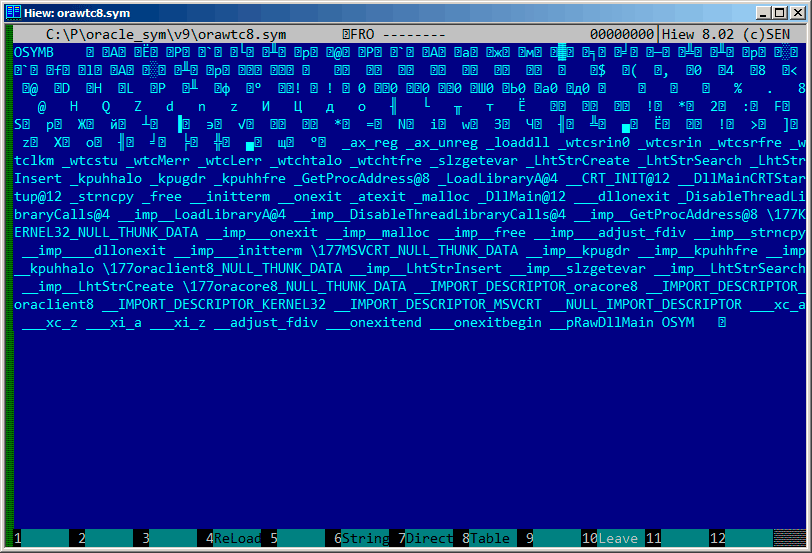
\includegraphics[scale=\FigScale]{examples/oracle/SYM/whole1.png}
\caption{\RU{Весь файл в Hiew}\EN{The whole file in Hiew}}
\label{fig:oracle_SYM_whole1}
\end{figure}

\begin{figure}[H]
\centering
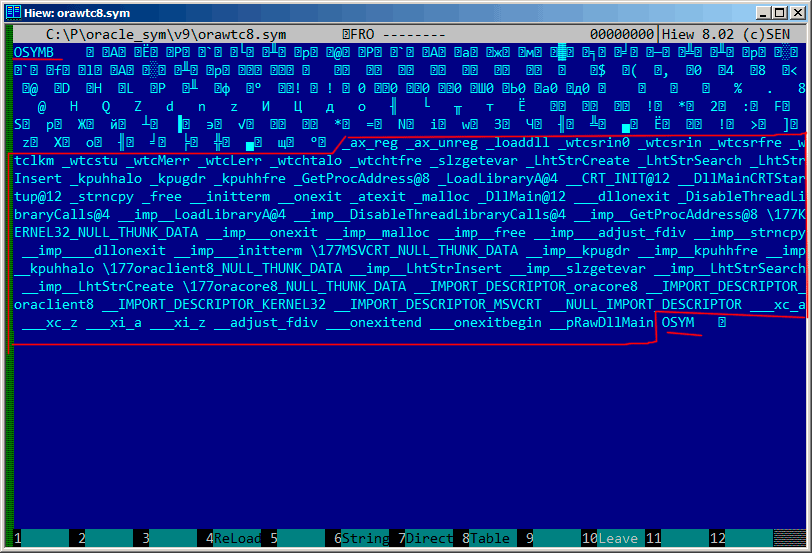
\includegraphics[scale=\FigScale]{examples/oracle/SYM/whole2.png}
\caption{\RU{Сигнатура OSYM и текстовые строки}\EN{OSYM signature and text strings}}
\label{fig:oracle_SYM_whole2}
\end{figure}

\begin{figure}[H]
\centering
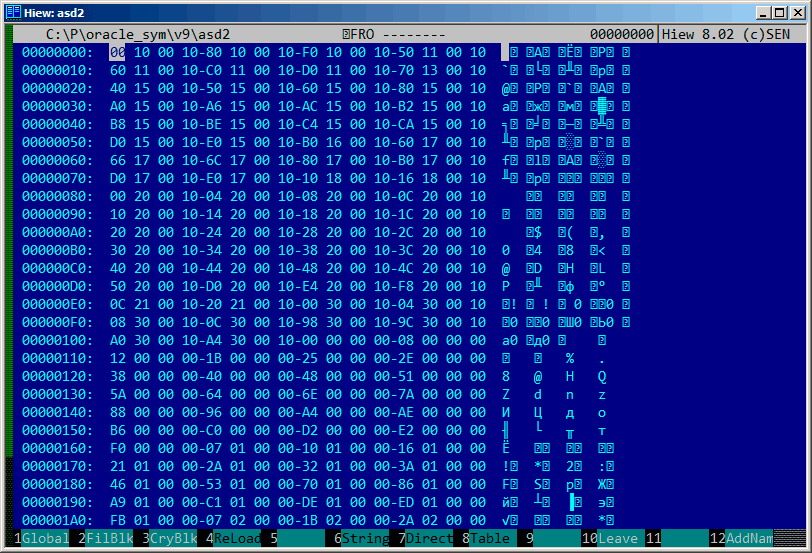
\includegraphics[scale=\FigScale]{examples/oracle/SYM/binary1.png}
\caption{\RU{Бинарный блок}\EN{Binary block}}
\label{fig:oracle_SYM_binary1}
\end{figure}

\begin{figure}[H]
\centering
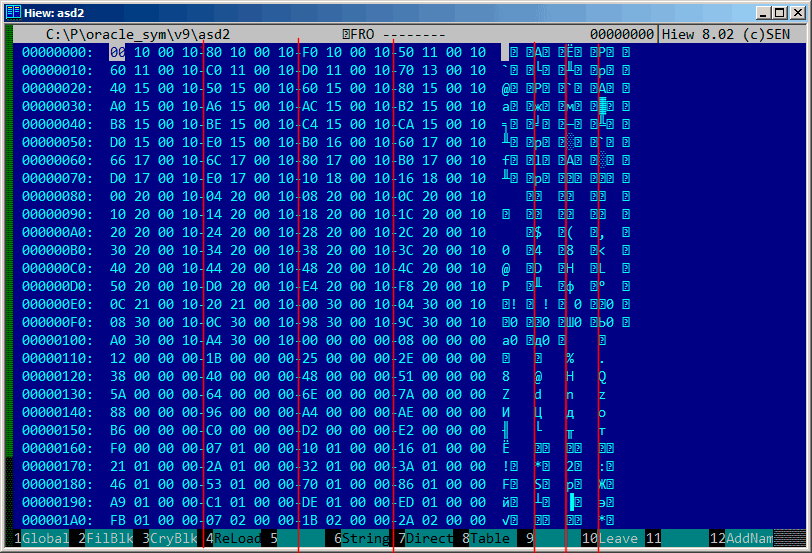
\includegraphics[scale=\FigScale]{examples/oracle/SYM/binary2.png}
\caption{\RU{Структура бинарного блока}\EN{Binary block patterns}}
\label{fig:oracle_SYM_binary2}
\end{figure}

\begin{figure}[H]
\centering
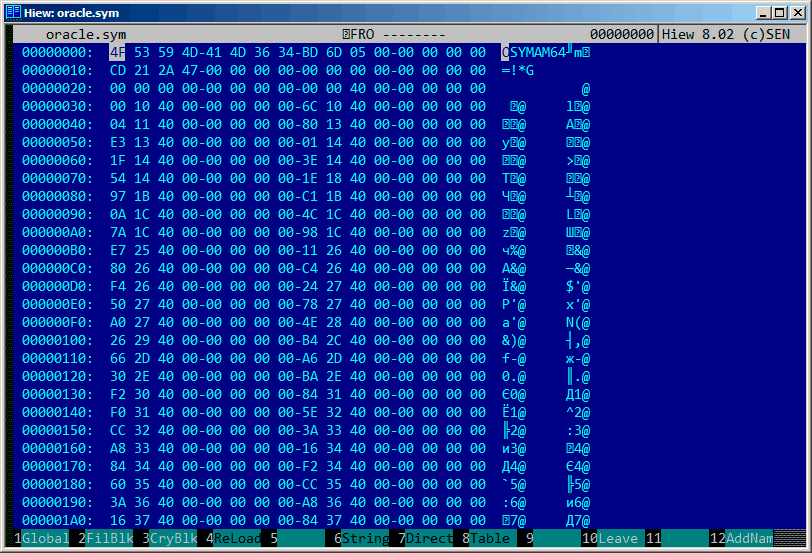
\includegraphics[scale=\FigScale]{examples/oracle/SYM/whole64.png}
\caption{\RU{пример .SYM-файла из \oracle для win64}\EN{.SYM-file example from \oracle for win64}}
\label{fig:oracle_SYM_whole64}
\end{figure}

\subsection{\IFRU{Таблица \TT{V\$VERSION} в \oracle}{\TT{V\$VERSION} table in the \oracle}}

\index{Oracle RDBMS}
\index{Linux}
\index{Windows!ntoskrnl.exe}
\IFRU{\oracle 11.2 это очень большая программа, основной модуль \TT{oracle.exe} содержит около 124 тысячи функций.}{\oracle 11.2 is a huge program, main module \TT{oracle.exe} contain approx. 124,000 functions.} \IFRU{Для сравнения, ядро Windows 7 x64 (ntoskrnl.exe) ~--- около 11 тысяч функций, а ядро Linux 3.9.8 (с драйверами по умолчанию) ~--- 31 тысяч функций.}{For comparison, Windows 7 x86 kernel (ntoskrnl.exe) ~--- approx. 11,000 functions and Linux 3.9.8 kernel (with default drivers compiled) ~--- 31,000 functions.}

\IFRU{Начнем с одного простого вопроса. Откуда \oracle берет информацию, когда мы в SQL*Plus пишем вот такой вот простой запрос:}{Let's start with an easy question. Where \oracle get all this information, when we execute such simple statement in SQL*Plus:}

\begin{lstlisting}
SQL> select * from V$VERSION;
\end{lstlisting}

\IFRU{И получаем}{And we've got}:

\begin{lstlisting}
BANNER
--------------------------------------------------------------------------------

Oracle Database 11g Enterprise Edition Release 11.2.0.1.0 - Production
PL/SQL Release 11.2.0.1.0 - Production
CORE    11.2.0.1.0      Production
TNS for 32-bit Windows: Version 11.2.0.1.0 - Production
NLSRTL Version 11.2.0.1.0 - Production
\end{lstlisting}

\IFRU{Начнем. Где в самом \oracle мы можем найти строку}{Let's start. Where in the \oracle we may find a string} \TT{V\$VERSION}?

\IFRU{Для win32-версии, эта строка имеется в файле \TT{oracle.exe}, это легко увидеть.}{As of win32-version, \TT{oracle.exe} file contain that string, that can be investigated easily.}
\IFRU{Но мы так же можем использовать объектные (.o) файлы от версии \oracle для Linux, потому что в них сохраняются имена функций и глобальных переменных, а в \TT{oracle.exe} для win32 этого нет.}{But we can also use object (.o) files from Linux version of \oracle since, unlike win32 version \TT{oracle.exe}, function names (and global variables as well) are preserved there.}

\IFRU{Итак, строка \TT{V\$VERSION} имеется в файле \TT{kqf.o}, в самой главной Oracle-библиотеке \TT{libserver11.a}.}{So, \TT{kqf.o} file contain \TT{V\$VERSION} string. That object file is in main Oracle-library \TT{libserver11.a}.}

\IFRU{Ссылка на эту текстовую строку имеется в таблице \TT{kqfviw}, размещенной в этом же файле \TT{kqf.o}}{A reference to this text string we may find in the \TT{kqfviw} table stored in the same file, \TT{kqf.o}}:

\begin{lstlisting}[caption=kqf.o]
.rodata:0800C4A0 kqfviw          dd 0Bh                  ; DATA XREF: kqfchk:loc_8003A6D
.rodata:0800C4A0                                         ; kqfgbn+34
.rodata:0800C4A4                 dd offset _2__STRING_10102_0 ; "GV$WAITSTAT"
.rodata:0800C4A8                 dd 4
.rodata:0800C4AC                 dd offset _2__STRING_10103_0 ; "NULL"
.rodata:0800C4B0                 dd 3
.rodata:0800C4B4                 dd 0
.rodata:0800C4B8                 dd 195h
.rodata:0800C4BC                 dd 4
.rodata:0800C4C0                 dd 0
.rodata:0800C4C4                 dd 0FFFFC1CBh
.rodata:0800C4C8                 dd 3
.rodata:0800C4CC                 dd 0
.rodata:0800C4D0                 dd 0Ah
.rodata:0800C4D4                 dd offset _2__STRING_10104_0 ; "V$WAITSTAT"
.rodata:0800C4D8                 dd 4
.rodata:0800C4DC                 dd offset _2__STRING_10103_0 ; "NULL"
.rodata:0800C4E0                 dd 3
.rodata:0800C4E4                 dd 0
.rodata:0800C4E8                 dd 4Eh
.rodata:0800C4EC                 dd 3
.rodata:0800C4F0                 dd 0
.rodata:0800C4F4                 dd 0FFFFC003h
.rodata:0800C4F8                 dd 4
.rodata:0800C4FC                 dd 0
.rodata:0800C500                 dd 5
.rodata:0800C504                 dd offset _2__STRING_10105_0 ; "GV$BH"
.rodata:0800C508                 dd 4
.rodata:0800C50C                 dd offset _2__STRING_10103_0 ; "NULL"
.rodata:0800C510                 dd 3
.rodata:0800C514                 dd 0
.rodata:0800C518                 dd 269h
.rodata:0800C51C                 dd 15h
.rodata:0800C520                 dd 0
.rodata:0800C524                 dd 0FFFFC1EDh
.rodata:0800C528                 dd 8
.rodata:0800C52C                 dd 0
.rodata:0800C530                 dd 4
.rodata:0800C534                 dd offset _2__STRING_10106_0 ; "V$BH"
.rodata:0800C538                 dd 4
.rodata:0800C53C                 dd offset _2__STRING_10103_0 ; "NULL"
.rodata:0800C540                 dd 3
.rodata:0800C544                 dd 0
.rodata:0800C548                 dd 0F5h
.rodata:0800C54C                 dd 14h
.rodata:0800C550                 dd 0
.rodata:0800C554                 dd 0FFFFC1EEh
.rodata:0800C558                 dd 5
.rodata:0800C55C                 dd 0
\end{lstlisting}

\IFRU{Кстати, нередко, при изучении внутренностей \oracle, появляется вопрос, почему имена функций и глобальных переменных такие странные}{By the way, often, while analysing \oracle internals, you may ask yourself, why functions and global variable names are so weird}. \IFRU{Вероятно, дело в том что \oracle очень старый продукт сам по себе и писался на Си еще в 1980-х}
{Supposedly, since \oracle is very old product and was developed in C in 1980-s}. \IFRU{А в те времена стандарт Си гарантировал поддержку имен переменных длиной только до шести символов включительно}{And that was a time when C standard guaranteed function names/variables support only up to 6 characters inclusive}: <<6 significant initial characters in an external identifier>>\footnote{\href{http://yurichev.com/ref/Draft\%20ANSI\%20C\%20Standard\%20(ANSI\%20X3J11-88-090)\%20(May\%2013,\%201988).txt}{Draft ANSI C Standard (ANSI X3J11/88-090) (May 13, 1988)}}

\IFRU{Вероятно, таблица \TT{kqfviw} содержащая в себе многие (а может даже и все) view с префиксом V\$, это служебные view (fixed views), присутствующие всегда.}{Probably, the table \TT{kqfviw} contain most (maybe even all) views prefixed with V\$, these are \IT{fixed views}, present all the time.}
\IFRU{Бегло оценив цикличность данных, мы легко видим что в каждом элементе таблицы \TT{kqfviw} 12 полей 32-битных полей.}{Superficially, by noticing cyclic recurrence of data, we can easily see that each \TT{kqfviw} table element has 12 32-bit fields.}
\IFRU{В \IDA легко создать структуру из 12-и элементов и применить её ко всем элементам таблицы.}{It is very simple to create a 12-elements structure in \IDA and apply it to all table elements.}
\IFRU{Для версии \oracle 11.2, здесь 1023 элемента в таблице, то есть, здесь описываются 1023 всех возможных \IT{fixed view}.}{As of \oracle version 11.2, there are 1023 table elements, i.e., there are described 1023 of all possible \IT{fixed views}.}
\IFRU{Позже, мы еще вернемся к этому числу.}{We will return to this number later.}

\IFRU{Как видно, мы не очень много можем узнать чисел в этих полях. Самое первое число всегда равно длине строки-названия view (без терминирующего ноля).}{As we can see, there are not much information in these numbers in fields. The very first number is always equals to name of view (without terminating zero.}
\IFRU{Это справедливо для всех элементов. Но эта информация не очень полезна.}{This is correct for each element. But this information is not very useful.}

\IFRU{Мы также знаем, что информацию обо всех fixed views можно получить из \IT{fixed view} под названием}{We also know that information about all fixed views can be retrieved from \IT{fixed view} named} \TT{V\$FIXED\_VIEW\_DEFINITION}
\IFRU{(кстати, информация для этого view также берется из таблиц \TT{kqfviw} и \TT{kqfvip}).}{(by the way, the information for this view is also taken from \TT{kqfviw} and \TT{kqfvip} tables.)}
\IFRU{Кстати, там тоже 1023 элемента.}{By the way, there are 1023 elemens too.}

\begin{lstlisting}
SQL> select * from V$FIXED_VIEW_DEFINITION where view_name='V$VERSION';

VIEW_NAME
------------------------------
VIEW_DEFINITION
--------------------------------------------------------------------------------

V$VERSION
select  BANNER from GV$VERSION where inst_id = USERENV('Instance')
\end{lstlisting}

\IFRU{Итак, \TT{V\$VERSION} это как бы \IT{thunk view} для другого, с названием \TT{GV\$VERSION}, который, в свою очередь:}{So, \TT{V\$VERSION} is some kind of \IT{thunk view} for another view, named \TT{GV\$VERSION}, which is, in turn:}

\begin{lstlisting}
SQL> select * from V$FIXED_VIEW_DEFINITION where view_name='GV$VERSION';

VIEW_NAME
------------------------------
VIEW_DEFINITION
--------------------------------------------------------------------------------

GV$VERSION
select inst_id, banner from x$version
\end{lstlisting}

\IFRU{Таблицы с префиксом X\$ в \oracle ~--- это также служебные таблицы, они не документированы, не могут изменятся пользователем, и обновляются динамически.}{Tables prefixed as X\$ in the \oracle -- is service tables too, undocumented, cannot be changed by user and refreshed dynamically.}

\IFRU{Попробуем поискать текст}{Let's also try to search the text} \TT{select  BANNER from GV\$VERSION where inst\_id = USERENV('Instance')} \IFRU{в файле \TT{kqf.o} и находим ссылку на него в таблице \TT{kqfvip}}{in the \TT{kqf.o} file and we find it in the \TT{kqfvip} table}:

.\begin{lstlisting}[caption=kqf.o]
rodata:080185A0 kqfvip          dd offset _2__STRING_11126_0 ; DATA XREF: kqfgvcn+18
.rodata:080185A0                                         ; kqfgvt+F
.rodata:080185A0                                         ; "select inst_id,decode(indx,1,'data bloc"...
.rodata:080185A4                 dd offset kqfv459_c_0
.rodata:080185A8                 dd 0
.rodata:080185AC                 dd 0

...

.rodata:08019570                 dd offset _2__STRING_11378_0 ; "select  BANNER from GV$VERSION where in"...
.rodata:08019574                 dd offset kqfv133_c_0
.rodata:08019578                 dd 0
.rodata:0801957C                 dd 0
.rodata:08019580                 dd offset _2__STRING_11379_0 ; "select inst_id,decode(bitand(cfflg,1),0"...
.rodata:08019584                 dd offset kqfv403_c_0
.rodata:08019588                 dd 0
.rodata:0801958C                 dd 0
.rodata:08019590                 dd offset _2__STRING_11380_0 ; "select  STATUS , NAME, IS_RECOVERY_DEST"...
.rodata:08019594                 dd offset kqfv199_c_0
\end{lstlisting}

\IFRU{Таблица, по всей видимости, имеет 4 поля в каждом элементе. Кстати, здесь также 1023 элемента.}
{The table appear to have 4 fields in each element. By the way, there are 1023 elements too.}
\IFRU{Второе поле указывает на другую таблицу, содержащую поля этого \IT{fixed view}.}
{The second field pointing to another table, containing table fields for this \IT{fixed view}.}
\IFRU{Для \TT{V\$VERSION}, эта таблица только из двух элементов, первый это $6$ и второй это строка 
\TT{BANNER} (число это длина строки) и далее \IT{терминирующий} элемент содержащий $0$ и \IT{нулевую} 
Си-строку:}{As of \TT{V\$VERSION}, this table contain only two elements, first is $6$ and second is 
\TT{BANNER} string (the number ($6$) is this string length) and after, \IT{terminating} element contain 
$0$ and \IT{null} C-string:}

\begin{lstlisting}[caption=kqf.o]
.rodata:080BBAC4 kqfv133_c_0     dd 6                    ; DATA XREF: .rodata:08019574
.rodata:080BBAC8                 dd offset _2__STRING_5017_0 ; "BANNER"
.rodata:080BBACC                 dd 0
.rodata:080BBAD0                 dd offset _2__STRING_0_0
\end{lstlisting}

\IFRU{Объеденив данные из таблиц \TT{kqfviw} и \TT{kqfvip}, мы получим SQL-запросы, которые исполняются, когда пользователь хочет получить информацию из какого-либо \IT{fixed view}.}{By joining data from both \TT{kqfviw} and \TT{kqfvip} tables, we may get SQL-statements which are executed when user wants to query information from specific \IT{fixed view}.}

\IFRU{Я написал программу \oracletables, которая собирает всю эту информацию из объектных файлов от \oracle под Linux.}{So I wrote an \oracletables program, so to gather all this information from \oracle for Linux object files.}
\IFRU{Для \TT{V\$VERSION}, мы можем найти следующее:}{For \TT{V\$VERSION}, we may find this:}

\begin{lstlisting}[caption=\IFRU{Результат работы}{Result of} \OracleTablesName]
kqfviw_element.viewname: [V$VERSION] ?: 0x3 0x43 0x1 0xffffc085 0x4
kqfvip_element.statement: [select  BANNER from GV$VERSION where inst_id = USERENV('Instance')]
kqfvip_element.params:
[BANNER] 
\end{lstlisting}

\AndENRU:

\begin{lstlisting}[caption=\IFRU{Результат работы}{Result of} \OracleTablesName]
kqfviw_element.viewname: [GV$VERSION] ?: 0x3 0x26 0x2 0xffffc192 0x1
kqfvip_element.statement: [select inst_id, banner from x$version]
kqfvip_element.params:
[INST_ID] [BANNER] 
\end{lstlisting}

\IFRU{\IT{Fixed view} \TT{GV\$VERSION} отличается от \TT{V\$VERSION} тем, что содержит еще и поле отражающее идентификатор \IT{instance}.}
{\TT{GV\$VERSION} \IT{fixed view} is distinct from \TT{V\$VERSION} in only that way that it contains one more field with \IT{instance} identifier.}
\IFRU{Но так или иначе, мы теперь упираемся в таблицу \TT{X\$VERSION}. Как и прочие X\$-таблицы, она недокументирована, однако, мы можем оттуда что-то прочитать}{Anyway, we stuck at the table \TT{X\$VERSION}. Just like any other X\$-tables, it is undocumented, however, we can query it}:

\begin{lstlisting}
SQL> select * from x$version;

ADDR           INDX    INST_ID
-------- ---------- ----------
BANNER
--------------------------------------------------------------------------------

0DBAF574          0          1
Oracle Database 11g Enterprise Edition Release 11.2.0.1.0 - Production

...
\end{lstlisting}

\IFRU{Эта таблица содержит дополнительные поля вроде \TT{ADDR} и \TT{INDX}.}{This table has additional fields like \TT{ADDR} and \TT{INDX}.}

\IFRU{Бегло листая содержимое файла \TT{kqf.o} в \IDA мы можем увидеть еще одну таблицу где есть ссылка на строку \TT{X\$VERSION}, это \TT{kqftab}:}{While scrolling \TT{kqf.o} in \IDA we may spot another table containing pointer to the \TT{X\$VERSION} string, this is \TT{kqftab}:}

\begin{lstlisting}[caption=kqf.o]
.rodata:0803CAC0                 dd 9                    ; element number 0x1f6
.rodata:0803CAC4                 dd offset _2__STRING_13113_0 ; "X$VERSION"
.rodata:0803CAC8                 dd 4
.rodata:0803CACC                 dd offset _2__STRING_13114_0 ; "kqvt"
.rodata:0803CAD0                 dd 4
.rodata:0803CAD4                 dd 4
.rodata:0803CAD8                 dd 0
.rodata:0803CADC                 dd 4
.rodata:0803CAE0                 dd 0Ch
.rodata:0803CAE4                 dd 0FFFFC075h
.rodata:0803CAE8                 dd 3
.rodata:0803CAEC                 dd 0
.rodata:0803CAF0                 dd 7
.rodata:0803CAF4                 dd offset _2__STRING_13115_0 ; "X$KQFSZ"
.rodata:0803CAF8                 dd 5
.rodata:0803CAFC                 dd offset _2__STRING_13116_0 ; "kqfsz"
.rodata:0803CB00                 dd 1
.rodata:0803CB04                 dd 38h
.rodata:0803CB08                 dd 0
.rodata:0803CB0C                 dd 7
.rodata:0803CB10                 dd 0
.rodata:0803CB14                 dd 0FFFFC09Dh
.rodata:0803CB18                 dd 2
.rodata:0803CB1C                 dd 0
\end{lstlisting}

\IFRU{Здесь очень много ссылок на названия X\$-таблиц, вероятно, на все те что имеются в \oracle этой версии.}{There are a lot of references to X\$-table names, apparently, to all \oracle 11.2 X\$-tables.}
\IFRU{Но мы снова упираемся в то что не имеем достаточно информации.}{But again, we have not enough information.}
\IFRU{У меня нет никакой идеи, что означает строка \TT{kqvt}.}
{I have no idea, what \TT{kqvt} string means.} 
\IFRU{Вообще, префикс \TT{kq} может означать \IT{kernel} и \IT{query}.}
{\TT{kq} prefix may means \IT{kernal} and \IT{query}.} 
\IFRU{\TT{v}, может быть, \IT{version}, а \TT{t} ~--- \IT{type}?}
{\TT{v}, apparently, means \IT{version} and \TT{t} ~--- \IT{type}?} 
\IFRU{Я не знаю, честно говоря.}{Frankly speaking, I do not know.}

\IFRU{Таблицу с очень похожим названием мы можем найти в}{The table named similarly can be found in} \TT{kqf.o}:

\begin{lstlisting}[caption=kqf.o]
.rodata:0808C360 kqvt_c_0        kqftap_param <4, offset _2__STRING_19_0, 917h, 0, 0, 0, 4, 0, 0>
.rodata:0808C360                                         ; DATA XREF: .rodata:08042680
.rodata:0808C360                                         ; "ADDR"
.rodata:0808C384                 kqftap_param <4, offset _2__STRING_20_0, 0B02h, 0, 0, 0, 4, 0, 0> ; "INDX"
.rodata:0808C3A8                 kqftap_param <7, offset _2__STRING_21_0, 0B02h, 0, 0, 0, 4, 0, 0> ; "INST_ID"
.rodata:0808C3CC                 kqftap_param <6, offset _2__STRING_5017_0, 601h, 0, 0, 0, 50h, 0, 0> ; "BANNER"
.rodata:0808C3F0                 kqftap_param <0, offset _2__STRING_0_0, 0, 0, 0, 0, 0, 0, 0>
\end{lstlisting}

\IFRU{Она содержит информацию об именах полей в таблице \TT{X\$VERSION}.}{It contain information about all fields in the \TT{X\$VERSION} table.}
\IFRU{Единственная ссылка на эту таблицу имеется в таблице \TT{kqftap}:}{The only reference to this table present in the \TT{kqftap} table:}

\begin{lstlisting}[caption=kqf.o]
.rodata:08042680                 kqftap_element <0, offset kqvt_c_0, offset kqvrow, 0> ; element 0x1f6
\end{lstlisting}

\IFRU{Интересно что здесь этот элемент проходит также под номером \TT{0x1f6} (502-й), как и ссылка на строку 
\TT{X\$VERSION} в таблице \TT{kqftab}.}
{It is interesting that this element here is \TT{0x1f6th} (502nd), just as a pointer to the \TT{X\$VERSION} string in 
the \TT{kqftab} table.}
\IFRU{Вероятно, таблицы \TT{kqftap} и \TT{kqftab} дополняют друг друга, как и \TT{kqfvip} и \TT{kqfviw}.}
{Probably, \TT{kqftap} and \TT{kqftab} tables are complement each other, just like \TT{kqfvip} and \TT{kqfviw}.}
\IFRU{Мы также видим здесь ссылку на функцию с названием \TT{kqvrow()}. А вот это уже кое-что!}
{We also see a pointer to the \TT{kqvrow()} function. Finally, we got something useful!}

\IFRU{Я сделал так чтобы моя программа \oracletables могла дампить и эти таблицы. Для \TT{X\$VERSION} получается:}
{So I added these tables to my \oracletables utility too. For \TT{X\$VERSION} I've got:}

\begin{lstlisting}[caption=\IFRU{Результат работы}{Result of} \OracleTablesName]
kqftab_element.name: [X$VERSION] ?: [kqvt] 0x4 0x4 0x4 0xc 0xffffc075 0x3
kqftap_param.name=[ADDR] ?: 0x917 0x0 0x0 0x0 0x4 0x0 0x0
kqftap_param.name=[INDX] ?: 0xb02 0x0 0x0 0x0 0x4 0x0 0x0
kqftap_param.name=[INST_ID] ?: 0xb02 0x0 0x0 0x0 0x4 0x0 0x0
kqftap_param.name=[BANNER] ?: 0x601 0x0 0x0 0x0 0x50 0x0 0x0
kqftap_element.fn1=kqvrow
kqftap_element.fn2=NULL
\end{lstlisting}

\IFRU{При помощи \tracer, можно легко проверить, что эта ф-ция вызывается 6 раз кряду (из ф-ции \TT{qerfxFetch()}) при получении строк из \TT{X\$VERSION}.}{With the help of \tracer, it is easy to check that this function called 6 times in row (from the \TT{qerfxFetch()} function) while querying \TT{X\$VERSION} table.}

\IFRU{Запустим \tracer в режиме \TT{cc} (он добавит комментарий к каждой исполненной инструкции):}{Let's run \tracer in the \TT{cc} mode (it will comment each executed instruction):}

\begin{lstlisting}
tracer -a:oracle.exe bpf=oracle.exe!_kqvrow,trace:cc
\end{lstlisting}

\lstinputlisting{examples/oracle/VERSION_kqvrow.asm}

\IFRU{Так можно легко увидеть, что номер строки таблицы задается извне. Сама ф-ция возвращает строку, формируя её так:}{Now it is easy to see that row number is passed from outside of function. The function returns the string constructing it as follows:}

\begin{center}
\begin{tabular}{ | l | l | }
\hline                        
\IFRU{Строка}{String} 1	& \IFRU{Использует глобальные переменные \TT{vsnstr}, \TT{vsnnum}, \TT{vsnban}. Вызывает \TT{sprintf()}.}{Using \TT{vsnstr}, \TT{vsnnum}, \TT{vsnban} global variables. Calling \TT{sprintf()}.} \\
\IFRU{Строка}{String} 2	& \IFRU{Вызывает}{Calling} \TT{kkxvsn()}. \\
\IFRU{Строка}{String} 3	& \IFRU{Вызывает}{Calling} \TT{lmxver()}. \\
\IFRU{Строка}{String} 4	& \IFRU{Вызывает}{Calling} \TT{npinli()}, \TT{nrtnsvrs()}. \\
\IFRU{Строка}{String} 5	& \IFRU{Вызывает}{Calling} \TT{lxvers()}. \\
\hline  
\end{tabular}
\end{center}

\IFRU{Так вызываются соответствующие ф-ции для определения номеров версий отдельных модулей.}{That's how corresponding functions are called for determining each module's version.}


\subsection{\IFRU{Таблица \TT{X\$KSMLRU} в}{\TT{X\$KSMLRU} table in} \oracle}
\index{Oracle RDBMS}

\IFRU{В заметке}{There is a mention of a special table in the} \IT{Diagnosing and Resolving Error ORA-04031 
on the Shared Pool or Other Memory Pools [Video] [ID 146599.1]} \IFRU{упоминается некая служебная таблица}{note}:

\begin{framed}
\begin{quotation}
There is a fixed table called X\$KSMLRU that tracks allocations in the shared pool that cause other objects 
in the shared pool to be aged out. This fixed table can be used to identify what is causing the large allocation.

If many objects are being periodically flushed from the shared pool then this will cause response time problems 
and will likely cause library cache latch contention problems when the objects are reloaded into the shared pool.

One unusual thing about the X\$KSMLRU fixed table is that the contents of the fixed table are erased whenever 
someone selects from the fixed table. This is done since the fixed table stores only the largest allocations 
that have occurred. The values are reset after being selected so that subsequent large allocations can be noted 
even if they were not quite as large as others that occurred previously. Because of this resetting, the output 
of selecting from this table should be carefully kept since it cannot be retrieved back after the query is issued.
\end{quotation}
\end{framed}

\IFRU{Однако, как можно легко убедиться, эта системная таблица очищается всякий раз, когда кто-то делает запрос 
к ней.}{However, as it can be easily checked, this table's contents is cleared each time table querying.}
\IFRU{Сможем ли мы найти причину, почему это происходит?}{Are we able to find why?}
\IFRU{Если вернуться к уже рассмотренным таблицам \TT{kqftab} и \TT{kqftap} полученных при помощи \oracletables, 
содержащим информацию о X\$-таблицах, мы узнаем что для того чтобы подготовить строки этой таблицы, 
вызывается ф-ция \TT{ksmlrs()}:}{Let's back to tables we already know: \TT{kqftab} and \TT{kqftap} 
which were generated with \oracletables help, containing all information about X\$-tables, now we can see here, 
the \TT{ksmlrs()} function is called to prepare this table's elements:}

\begin{lstlisting}[caption=\IFRU{Результат работы}{Result of} \OracleTablesName]
kqftab_element.name: [X$KSMLRU] ?: [ksmlr] 0x4 0x64 0x11 0xc 0xffffc0bb 0x5
kqftap_param.name=[ADDR] ?: 0x917 0x0 0x0 0x0 0x4 0x0 0x0
kqftap_param.name=[INDX] ?: 0xb02 0x0 0x0 0x0 0x4 0x0 0x0
kqftap_param.name=[INST_ID] ?: 0xb02 0x0 0x0 0x0 0x4 0x0 0x0
kqftap_param.name=[KSMLRIDX] ?: 0xb02 0x0 0x0 0x0 0x4 0x0 0x0
kqftap_param.name=[KSMLRDUR] ?: 0xb02 0x0 0x0 0x0 0x4 0x4 0x0
kqftap_param.name=[KSMLRSHRPOOL] ?: 0xb02 0x0 0x0 0x0 0x4 0x8 0x0
kqftap_param.name=[KSMLRCOM] ?: 0x501 0x0 0x0 0x0 0x14 0xc 0x0
kqftap_param.name=[KSMLRSIZ] ?: 0x2 0x0 0x0 0x0 0x4 0x20 0x0
kqftap_param.name=[KSMLRNUM] ?: 0x2 0x0 0x0 0x0 0x4 0x24 0x0
kqftap_param.name=[KSMLRHON] ?: 0x501 0x0 0x0 0x0 0x20 0x28 0x0
kqftap_param.name=[KSMLROHV] ?: 0xb02 0x0 0x0 0x0 0x4 0x48 0x0
kqftap_param.name=[KSMLRSES] ?: 0x17 0x0 0x0 0x0 0x4 0x4c 0x0
kqftap_param.name=[KSMLRADU] ?: 0x2 0x0 0x0 0x0 0x4 0x50 0x0
kqftap_param.name=[KSMLRNID] ?: 0x2 0x0 0x0 0x0 0x4 0x54 0x0
kqftap_param.name=[KSMLRNSD] ?: 0x2 0x0 0x0 0x0 0x4 0x58 0x0
kqftap_param.name=[KSMLRNCD] ?: 0x2 0x0 0x0 0x0 0x4 0x5c 0x0
kqftap_param.name=[KSMLRNED] ?: 0x2 0x0 0x0 0x0 0x4 0x60 0x0
kqftap_element.fn1=ksmlrs
kqftap_element.fn2=NULL
\end{lstlisting}

\IFRU{Действительно, при помощи \tracer легко убедиться что эта ф-ция вызывается каждый раз, когда мы обращаемся 
к таблице \TT{X\$KSMLRU}.}{Indeed, with the \tracer help it is easy to see that this function is called each 
time we query the \TT{X\$KSMLRU} table.}

\IFRU{Здесь есть ссылки на ф-ции \TT{ksmsplu\_sp()} и \TT{ksmsplu\_jp()}, каждая из которых в итоге вызывает 
\TT{ksmsplu()}.}{Here we see a references to the \TT{ksmsplu\_sp()} and \TT{ksmsplu\_jp()} functions, each of 
them call the \TT{ksmsplu()} finally.}
\IFRU{В конце ф-ции \TT{ksmsplu()} мы видим вызов \TT{memset()}:}{At the end of the \TT{ksmsplu()} function we see 
a call to the \TT{memset()}:}

\begin{lstlisting}[caption=ksm.o]
...

.text:00434C50 loc_434C50:                             ; DATA XREF: .rdata:off_5E50EA8
.text:00434C50                 mov     edx, [ebp-4]
.text:00434C53                 mov     [eax], esi
.text:00434C55                 mov     esi, [edi]
.text:00434C57                 mov     [eax+4], esi
.text:00434C5A                 mov     [edi], eax
.text:00434C5C                 add     edx, 1
.text:00434C5F                 mov     [ebp-4], edx
.text:00434C62                 jnz     loc_434B7D
.text:00434C68                 mov     ecx, [ebp+14h]
.text:00434C6B                 mov     ebx, [ebp-10h]
.text:00434C6E                 mov     esi, [ebp-0Ch]
.text:00434C71                 mov     edi, [ebp-8]
.text:00434C74                 lea     eax, [ecx+8Ch]
.text:00434C7A                 push    370h            ; Size
.text:00434C7F                 push    0               ; Val
.text:00434C81                 push    eax             ; Dst
.text:00434C82                 call    __intel_fast_memset
.text:00434C87                 add     esp, 0Ch
.text:00434C8A                 mov     esp, ebp
.text:00434C8C                 pop     ebp
.text:00434C8D                 retn
.text:00434C8D _ksmsplu        endp
\end{lstlisting}

\index{\CStandardLibrary!memset()}
\IFRU{Такие конструкции (\TT{memset (block, 0, size)}) очень часто используются для простого обнуления блока памяти.}{Constructions like \TT{memset (block, 0, size)} are often used just to zero memory block.}
\IFRU{Мы можем попробовать рискнуть, заблокировав вызов \TT{memset()} и посмотреть, что будет?}{What if we would take a risk, block \TT{memset()} call and see what will happen?}

\IFRU{Запускаем \tracer со следующей опцией: поставить точку останова на \TT{0x434C7A} (там где начинается передача 
параметров для ф-ции \TT{memset()}) так, чтобы \tracer в этом месте установил указатель инструкций процессора (\TT{EIP}) на место, где уже произошла очистка переданных параметров в \TT{memset()} (по адресу \TT{0x434C8A}):}
{Let's run \tracer with the following options: set breakpoint at \TT{0x434C7A} (the point where \TT{memset()} arguments are to be passed), thus, that \tracer set program counter \TT{EIP} at this point to the point where passed to the \TT{memset()} arguments are to be cleared (at \TT{0x434C8A})}
\IFRU{Можно сказать, при помощи этого, мы симулируем безусловный переход с адреса}{It can be said, we just simulate an unconditional jump from the address} \TT{0x434C7A} \IFRU{на}{to} \TT{0x434C8A}.

\begin{lstlisting}
tracer -a:oracle.exe bpx=oracle.exe!0x00434C7A,set(eip,0x00434C8A)
\end{lstlisting}

\IFRU{(Важно: все эти адреса справедливы только для win32-версии \oracle 11.2)}{(Important: all these addresses are valid only for win32-version of \oracle 11.2)}

\IFRU{Действительно, после этого мы можем обращаться к таблице \TT{X\$KSMLRU} сколько угодно, и она уже не очищается!}{Indeed, now we can query \TT{X\$KSMLRU} table as many times as we want and it is not clearing anymore!}

\IFRU{\sout{Не делайте этого дома ("Разрушители легенд")} Не делайте этого на своих production-серверах.}{\sout{Do not try this at home ("MythBusters")} Do not try this on your production servers.}

\IFRU{Впрочем, это не обязательно полезное или желаемое поведение системы, но как эксперимент по поиску нужного кода, нам это подошло!}{It is probably not a very useful or desired system behaviour, but as an experiment of locating piece of code we need, that is perfectly suit our needs!}


\section{\RU{Таблица \TT{V\$TIMER} в}\EN{\TT{V\$TIMER} table in} \oracle}
\index{\oracle}

\TT{V\$TIMER} \RU{это еще один служебный \IT{fixed view}, отражающий какое-то часто меняющееся значение:}
\EN{is another \IT{fixed view} that reflects a rapidly changing value:}

\begin{framed}
\begin{quotation}
V\$TIMER displays the elapsed time in hundredths of a second. Time is measured since the beginning of the epoch, 
which is operating system specific, and wraps around to 0 again whenever the value overflows four bytes 
(roughly 497 days).
\end{quotation}
\end{framed}(\RU{Из документации \oracle}\EN{From \oracle documentation}
\footnote{\url{http://go.yurichev.com/17088}})

\RU{Интересно что периоды разные в Oracle для Win32 и для Linux. Сможем ли мы найти функцию, отвечающую 
за генерирование этого значения?}
\EN{It is interesting that the periods are different for Oracle for win32 and for Linux. 
Will we be able to find the function that generates this value?}

\RU{Как видно, эта информация, в итоге, берется из системной таблицы \TT{X\$KSUTM}.}\EN{As we can see, 
this information is finally taken from the \TT{X\$KSUTM} table.}

\begin{lstlisting}
SQL> select * from V$FIXED_VIEW_DEFINITION where view_name='V$TIMER';

VIEW_NAME
------------------------------
VIEW_DEFINITION
--------------------------------------------------------------------------------

V$TIMER
select  HSECS from GV$TIMER where inst_id = USERENV('Instance')

SQL> select * from V$FIXED_VIEW_DEFINITION where view_name='GV$TIMER';

VIEW_NAME
------------------------------
VIEW_DEFINITION
--------------------------------------------------------------------------------

GV$TIMER
select inst_id,ksutmtim from x$ksutm
\end{lstlisting}

\RU{Здесь мы упираемся в небольшую проблему, в таблицах \TT{kqftab}/\TT{kqftap} нет указателей на функцию, 
которая бы генерировала значение}
\EN{Now we are stuck in a small problem, there are no references to value generating function(s) 
in the tables \TT{kqftab}/\TT{kqftap}}:

\begin{lstlisting}[caption=\RU{Результат работы}\EN{Result of} \OracleTablesName]
kqftab_element.name: [X$KSUTM] ?: [ksutm] 0x1 0x4 0x4 0x0 0xffffc09b 0x3
kqftap_param.name=[ADDR] ?: 0x10917 0x0 0x0 0x0 0x4 0x0 0x0
kqftap_param.name=[INDX] ?: 0x20b02 0x0 0x0 0x0 0x4 0x0 0x0
kqftap_param.name=[INST_ID] ?: 0xb02 0x0 0x0 0x0 0x4 0x0 0x0
kqftap_param.name=[KSUTMTIM] ?: 0x1302 0x0 0x0 0x0 0x4 0x0 0x1e
kqftap_element.fn1=NULL
kqftap_element.fn2=NULL
\end{lstlisting}

\RU{Попробуем в таком случае просто поискать строку \TT{KSUTMTIM}, и находим ссылку на нее в такой функции:}
\EN{When we try to find the string \TT{KSUTMTIM}, we see it in this function:}

\begin{lstlisting}
kqfd_DRN_ksutm_c proc near              ; DATA XREF: .rodata:0805B4E8

arg_0           = dword ptr  8
arg_8           = dword ptr  10h
arg_C           = dword ptr  14h

                push    ebp
                mov     ebp, esp
                push    [ebp+arg_C]
                push    offset ksugtm
                push    offset _2__STRING_1263_0 ; "KSUTMTIM"
                push    [ebp+arg_8]
                push    [ebp+arg_0]
                call    kqfd_cfui_drain
                add     esp, 14h
                mov     esp, ebp
                pop     ebp
                retn
kqfd_DRN_ksutm_c endp
\end{lstlisting}

\RU{Сама функция}\EN{The} \TT{kqfd\_DRN\_ksutm\_c()} \RU{упоминается в таблице}\EN{function is mentioned in the} 
\TT{kqfd\_tab\_registry\_0} \RU{вот так}\EN{table}:

\begin{lstlisting}
dd offset _2__STRING_62_0 ; "X$KSUTM"
dd offset kqfd_OPN_ksutm_c
dd offset kqfd_tabl_fetch
dd 0
dd 0
dd offset kqfd_DRN_ksutm_c
\end{lstlisting}

\RU{Упоминается также некая функция \TT{ksugtm()}}\EN{There is a function \TT{ksugtm()} referenced here}.
\RU{Посмотрим, что там (в Linux x86)}\EN{Let's see what's in it (Linux x86)}:

\begin{lstlisting}[caption=ksu.o]
ksugtm          proc near

var_1C          = byte ptr -1Ch
arg_4           = dword ptr  0Ch

                push    ebp
                mov     ebp, esp
                sub     esp, 1Ch
                lea     eax, [ebp+var_1C]
                push    eax
                call    slgcs
                pop     ecx
                mov     edx, [ebp+arg_4]
                mov     [edx], eax
                mov     eax, 4
                mov     esp, ebp
                pop     ebp
                retn
ksugtm          endp
\end{lstlisting}

\RU{В win32-версии тоже самое}\EN{The code in the win32 version is almost the same}.

\RU{Искомая ли эта функция? Попробуем узнать}\EN{Is this the function we are looking for? Let's see}:
\index{tracer}

\begin{lstlisting}
tracer -a:oracle.exe bpf=oracle.exe!_ksugtm,args:2,dump_args:0x4
\end{lstlisting}

\RU{Пробуем несколько раз}\EN{Let's try again}:

\begin{lstlisting}
SQL> select * from V$TIMER;

     HSECS
----------
  27294929

SQL> select * from V$TIMER;

     HSECS
----------
  27295006

SQL> select * from V$TIMER;

     HSECS
----------
  27295167
\end{lstlisting}

\begin{lstlisting}[caption=\RU{вывод \tracer}\EN{\tracer output}]
TID=2428|(0) oracle.exe!_ksugtm (0x0, 0xd76c5f0) (called from oracle.exe!__VInfreq__qerfxFetch+0xfad (0x56bb6d5))
Argument 2/2
0D76C5F0: 38 C9                                           "8.              "
TID=2428|(0) oracle.exe!_ksugtm () -> 0x4 (0x4)
Argument 2/2 difference
00000000: D1 7C A0 01                                     ".|..            "
TID=2428|(0) oracle.exe!_ksugtm (0x0, 0xd76c5f0) (called from oracle.exe!__VInfreq__qerfxFetch+0xfad (0x56bb6d5))
Argument 2/2
0D76C5F0: 38 C9                                           "8.              "
TID=2428|(0) oracle.exe!_ksugtm () -> 0x4 (0x4)
Argument 2/2 difference
00000000: 1E 7D A0 01                                     ".}..            "
TID=2428|(0) oracle.exe!_ksugtm (0x0, 0xd76c5f0) (called from oracle.exe!__VInfreq__qerfxFetch+0xfad (0x56bb6d5))
Argument 2/2
0D76C5F0: 38 C9                                           "8.              "
TID=2428|(0) oracle.exe!_ksugtm () -> 0x4 (0x4)
Argument 2/2 difference
00000000: BF 7D A0 01                                     ".}..            "
\end{lstlisting}

\RU{Действительно\EMDASH{}значение то, что мы видим в SQL*Plus, и оно возвращается через второй аргумент}
\EN{Indeed\EMDASH{}the value is the same we see in SQL*Plus and it is returned via the second argument}.

\RU{Посмотрим, что в функции}\EN{Let's see what is in} \TT{slgcs()} (Linux x86):

\begin{lstlisting}
slgcs           proc near

var_4           = dword ptr -4
arg_0           = dword ptr  8

                push    ebp
                mov     ebp, esp
                push    esi
                mov     [ebp+var_4], ebx
                mov     eax, [ebp+arg_0]
                call    $+5
                pop     ebx
                nop                     ; PIC mode
                mov     ebx, offset _GLOBAL_OFFSET_TABLE_
                mov     dword ptr [eax], 0
                call    sltrgatime64    ; PIC mode
                push    0
                push    0Ah
                push    edx
                push    eax
                call    __udivdi3       ; PIC mode
                mov     ebx, [ebp+var_4]
                add     esp, 10h
                mov     esp, ebp
                pop     ebp
                retn
slgcs           endp
\end{lstlisting}

(\RU{это просто вызов}\EN{it is just a call to} \TT{sltrgatime64()} \RU{и деление его результата на}
\EN{and division of its result by} 10~(\myref{sec:divisionbynine}))

\RU{И в win32-версии}\EN{And win32-version}:

\begin{lstlisting}
_slgcs          proc near               ; CODE XREF: _dbgefgHtElResetCount+15
                                        ; _dbgerRunActions+1528
                db      66h
                nop
                push    ebp
                mov     ebp, esp
                mov     eax, [ebp+8]
                mov     dword ptr [eax], 0
                call    ds:__imp__GetTickCount@0 ; GetTickCount()
                mov     edx, eax
                mov     eax, 0CCCCCCCDh
                mul     edx
                shr     edx, 3
                mov     eax, edx
                mov     esp, ebp
                pop     ebp
                retn
_slgcs          endp
\end{lstlisting}

\RU{Это просто результат}\EN{It is just the result of} \TT{GetTickCount()
\footnote{\href{http://go.yurichev.com/17248}{MSDN}}} 
\RU{поделенный на}\EN{divided by} 10~(\myref{sec:divisionbynine}).

\RU{Вуаля! Вот почему в win32-версии и версии Linux x86 разные результаты, потому что они получаются разными 
системными функциями \ac{OS}.}\EN{Voilà! That's why the win32 version and the Linux x86 version show different results, 
because they are generated by different \ac{OS} functions.}

\RU{\IT{Drain} по-английски \IT{дренаж, отток, водосток}. Таким образом, возможно имеется ввиду \IT{подключение} 
определенного столбца системной таблице к функции.}
\EN{\IT{Drain} apparently implies \IT{connecting} a specific table column to a specific function.}

\RU{Добавим поддержку таблицы}\EN{We will add support of the table} \TT{kqfd\_tab\_registry\_0} \RU{в}\EN{to} \oracletables, 
\RU{теперь мы можем видеть, при помощи каких функций, столбцы в системных таблицах \IT{подключаются} к значениям, 
например}\EN{now we can see how the table column's variables are \IT{connected} to a specific functions}:

\begin{lstlisting}
[X$KSUTM] [kqfd_OPN_ksutm_c] [kqfd_tabl_fetch] [NULL] [NULL] [kqfd_DRN_ksutm_c]
[X$KSUSGIF] [kqfd_OPN_ksusg_c] [kqfd_tabl_fetch] [NULL] [NULL] [kqfd_DRN_ksusg_c]
\end{lstlisting}

\IT{OPN}, \RU{возможно}\EN{apparently stands for}, \IT{open}, \RU{а}\EN{and} \IT{DRN}, \RU{вероятно, означает}
\EN{apparently, for} \IT{drain}.



\EN{\chapterold{Handwritten assembly code}

\sectionold{ EICAR test file}
\label{subsec:EICAR}

\myindex{MS-DOS}
\myindex{EICAR}
This .COM-file is intended for testing antivirus software, it is possible to run in
in MS-DOS and it prints this string: \q{EICAR-STANDARD-ANTIVIRUS-TEST-FILE!}
\footnote{\href{http://go.yurichev.com/17006}{wikipedia}}.
% FIXME1 \myref{} -> about .COM files

Its important property is that it's consists entirely of printable 
ASCII-symbols, which, in turn, makes it possible to create it in any text editor:

\begin{lstlisting}
X5O!P%@AP[4\PZX54(P^)7CC)7}$EICAR-STANDARD-ANTIVIRUS-TEST-FILE!$H+H*
\end{lstlisting}

Let's decompile it:

\lstinputlisting{examples/handcoding/EICAR_EN.lst}

%
We will add comments about the registers and stack after each instruction.

Essentially, all these
instructions are here only to execute this code:

\begin{lstlisting}
B4 09     MOV AH, 9
BA 1C 01  MOV DX, 11Ch
CD 21     INT 21h
CD 20     INT 20h
\end{lstlisting}

\myindex{x86!\Instructions!INT}
\TT{INT 21h} with 9th
function (passed in \TT{AH}) just prints a string, the address of which is passed in \TT{DS:DX}.
By the way, the string has to be terminated
with the '\$' sign.
Apparently, it's inherited from \gls{CP/M} 
and this function was left in DOS for compatibility.
\TT{INT 20h} exits to DOS.

But as we can see, these instruction's
opcodes are not strictly printable.
So the main part of EICAR file is:

\begin{itemize}
\item preparing the register (AH and DX) values that we need;
\item preparing INT 21 and INT 20 opcodes in memory;
\item executing INT 21 \AndENRU INT 20.
\end{itemize}

\myindex{Shellcode}

By the way, this technique is widely used in shellcode construction, when one need to pass x86 code
in string form.

Here is also a list of all 
x86 instructions which have printable opcodes: \myref{printable_x86_opcodes}.
}\RU{\chapterold{Вручную написанный на ассемблере код}

\sectionold{Тестовый файл EICAR}
\label{subsec:EICAR}

\myindex{MS-DOS}
\myindex{EICAR}
Этот .COM-файл предназначен для тестирования антивирусов, его можно запустить в MS-DOS
и он выведет такую строку: \q{EICAR-STANDARD-ANTIVIRUS-TEST-FILE!}
\footnote{\href{http://go.yurichev.com/17005}{wikipedia}}.
% FIXME1 \myref{} -> about .COM files

Он примечателен тем, что он полностью состоит только из печатных ASCII-символов, следовательно, его можно
набрать в любом текстовом редакторе:

\begin{lstlisting}
X5O!P%@AP[4\PZX54(P^)7CC)7}$EICAR-STANDARD-ANTIVIRUS-TEST-FILE!$H+H*
\end{lstlisting}

Попробуем его разобрать:

\lstinputlisting{examples/handcoding/EICAR_RU.lst}

Добавим везде комментарии, показывающие состояние регистров и стека после каждой инструкции%
.

Собственно, все эти инструкции нужны только для того чтобы исполнить следующий код:

\begin{lstlisting}
B4 09     MOV AH, 9
BA 1C 01  MOV DX, 11Ch
CD 21     INT 21h
CD 20     INT 20h
\end{lstlisting}

\myindex{x86!\Instructions!INT}
\TT{INT 21h} с функцией 9 (переданной в \TT{AH}) просто выводит строку, адрес которой передан в \TT{DS:DX}.
Кстати, строка должна быть завершена символом '\$'.
Вероятно, это наследие \gls{CP/M} 
и эта функция в DOS осталась для совместимости.
\TT{INT 20h} возвращает управление в DOS.

Но, как видно, далеко не все опкоды этих инструкций печатные.
Так что основная часть EICAR-файла это:

\begin{itemize}
\item подготовка нужных значений регистров (AH и DX);
\item подготовка в памяти опкодов для INT 21 и INT 20;
\item исполнение INT 21 \AndENRU INT 20.
\end{itemize}

\myindex{Shellcode}
Кстати, подобная техника широко используется для создания шеллкодов, 
где нужно создать x86-код, который будет нужно передать в виде текстовой строки
.

Здесь также список всех x86-инструкций с печатаемыми опкодоами: \myref{printable_x86_opcodes}.
}
\section{\IFRU{Демо}{Demos}}

\IFRU{Демо (или демомейкинг) были великолепным упражнением в математике, программировании компьютерной графики
и очень плотному программированию на ассемблере вручную}{Demos (or demomaking) was an excellent 
exercise in mathematics, computer graphics programming and very tight x86 hand coding}.

\section{10 PRINT CHR\$(205.5+RND(1)); : GOTO 10}

\RU{Все примеры здесь для .COM-файлов под MS-DOS}\EN{All examples here are MS-DOS .COM files}.
%FIXME1 -> about .COM files

\index{MS-DOS}
\RU{В}\EN{In} \cite{10PRINT} \RU{можно прочитать об одном из простейших генераторов случайных лабиринтов}
\EN{we can read about one of the most simple possible random maze generators}.
\RU{Он просто бесконечно и случайно печатает символ слэша или обратный слэша, выдавая в итоге что-то вроде}
\EN{It just prints a slash or backslash characters randomly and endlessly, resulting in something like this}:

\begin{figure}[H]
\centering

\includegraphics[scale=\NormalScale]{examples/demos/10print/10print.png}
\end{figure}

\RU{Здесь несколько известных реализаций для 16-битного x86}
\EN{There are a few known implementations for 16-bit x86}.

\subsection{\RU{Версия 42-х байт от Trixter}\EN{Trixter's 42 byte version}}

\newcommand{\FNURLTRIXTER}{\footnote{\url{http://go.yurichev.com/17305}}}

\RU{Листинг взят с его сайта}\EN{The listing was taken from his website}\FNURLTRIXTER, \RU{но комментарии\EMDASH{}мои}
\EN{but the comments are mine}.

\lstinputlisting{examples/demos/10print/10print_42.lst.\LANG}

\index{Intel!8253}
\RU{Псевдослучайное число на самом деле это время, прошедшее со старта системы, получаемое из чипа таймера 8253, 
это значение
увеличивается на единицу 18.2 раза в секунду}\EN{The pseudo-random value here is in fact the time 
that has passed from the system's boot, taken from the 8253 time chip, the value increases by one 18.2 times per second}.

\RU{Записывая ноль в порт}\EN{By writing zero to port} \TT{43h}, 
\RU{мы имеем ввиду что команда это}\EN{we send the command} \q{\RU{выбрать счетчик}\EN{select counter} 0}, 
"counter latch", 
"\RU{двоичный счетчик}\EN{binary counter}" (\RU{а не значение \ac{BCD}}\EN{not a \ac{BCD} value}).

\index{x86!\Instructions!POPF}
\RU{Прерывания снова разрешаются при помощи инструкции}\EN{The interrupts are enabled back with the} \TT{POPF}\RU{, которая
также возвращает флаг \TT{IF}}\EN{ instruction, which restores the \TT{IF} flag as well}.

\index{x86!\Instructions!IN}
\RU{Инструкцию \TT{IN} нельзя использовать с другими регистрами кроме}\EN{It is not possible to 
use the \TT{IN} instruction with registers other than} \TT{AL}, \RU{поэтому здесь перетасовка}
\EN{hence the shuffling}.

\subsection{\RU{Моя попытка укоротить версию Trixter: 27 байт}
\EN{My attempt to reduce Trixter's version: 27 bytes}}

\RU{Мы можем сказать, что мы используем таймер не для того чтобы получить точное время, но псевдослучайное число,
так что мы можем не тратить время (и код) на запрещение прерываний}\EN{We can say that since we use the timer not 
to get a precise time value, but a pseudo-random one, we do not need
to spend time (and code) to disable the interrupts}.
\RU{Еще можно сказать, что так как мы берем бит из младшей 8-битной части, то мы можем считывать только её}
\EN{Another thing we can say is that we need only one bit from the low 8-bit part, so let's read only it}.

\RU{Немного укоротим код и выходит 27 байт}\EN{We can reduced the code slightly and we've got 27 bytes}:

\lstinputlisting{examples/demos/10print/10print_27.lst.\LANG}

\subsection{\RU{Использование случайного мусора в памяти как источника случайных чисел}
\EN{Taking random memory garbage as a source of randomness}}

\RU{Так как это}\EN{Since it is} MS-DOS, \RU{защиты памяти здесь нет вовсе, так что мы можем читать с какого
угодно адреса}\EN{there is no memory protection at all, we can read from whatever address we want}.
\index{x86!\Instructions!LODSB}
\RU{И даже более того: простая инструкция}\EN{Even more than that: a simple} \TT{LODSB} 
\RU{будет читать байт по адресу}\EN{instruction reads a byte from the} \TT{DS:SI}\RU{, но это не проблема
если правильные значения не установлены в регистры, пусть она читает 1) случайные байты; 2) из случайного
места в памяти!}\EN{ address, but it's not a problem
if the registers' values are not set up, let it read 1) random bytes; 2) from a random place in memory!}

\RU{Так что на странице Trixter-а}\EN{It is suggested in Trixter's webpage}\FNURLTRIXTER 
\RU{можно найти предложение использовать}\EN{to use} \TT{LODSB} \RU{без всякой инициализации}\EN{without any setup}.

\index{x86!\Instructions!SCASB}
\RU{Есть также предложение использовать инструкцию}\EN{It is also suggested that the} \TT{SCASB} 
\RU{вместо, потому что она выставляет флаги в соответствии с прочитанным значением}
\EN{instruction can be used instead, because it sets a flag according to the byte it reads}.

\RU{Еще одна идея насчет минимизации кода\EMDASH{}это использовать прерывание DOS}
\EN{Another idea to minimize the code is to use the} \TT{INT 29h} \RU{которое просто печатает символ на экране
из регистра}\EN{DOS syscall, which just prints the character stored in the} \TT{AL}\EN{ register}.

\RU{Это то что сделали}\EN{That is what} Peter Ferrie \AndENRU \HERMIT{}\EN{ did} (11 \AndENRU 
10 \RU{байт}\EN{bytes})
\footnote{\url{http://go.yurichev.com/17087}}:

\lstinputlisting[caption=\HERMIT: 11 \RU{байт}\EN{bytes}]{examples/demos/10print/herm1t_11.lst.\LANG}

\index{x86!\Instructions!SCASB}
\TT{SCASB} \RU{также использует значение в регистре}\EN{also uses the value in the} \TT{AL}\RU{, она вычитает значение
случайного байта в памяти из}
\EN{ register, it subtract a random memory byte's value from the} \TT{5Ch} \RU{в}\EN{value in} \TT{AL}.
\index{x86!\Instructions!JP}
\TT{JP} \RU{это редкая инструкция, здесь она используется для проверки флага четности (PF),
который вычисляется по формуле в листинге}\EN{is a rare instruction, here it used for checking the parity flag (PF), 
which is generated by the formulae in the listing}.
\RU{Как следствие, выводимый символ определяется не каким-то конкретным битом из случайного байта в памяти,
а суммой бит, и это (надеемся) сделает результат более распределенным}\EN{As a consequence, the output character 
is determined not by some bit in a random memory byte, but by a sum of bits, 
this (hopefully) makes the result more distributed}.

\index{x86!\Instructions!SALC}
\index{x86!\Instructions!SETALC}
\index{NEC V20}
\RU{Можно сделать еще короче, если использовать недокументированную x86-инструкцию}\EN{It is possible to 
make this even shorter by using the undocumented x86 instruction} \TT{SALC} (\ac{AKA} \TT{SETALC}) (\q{Set AL CF}).
\RU{Она появилась в}\EN{It was introduced in the NEC V20} \ac{CPU} \RU{и выставляет}\EN{and sets} \TT{AL} \RU{в}\EN{to} 
\TT{0xFF} \RU{если}\EN{if} \TT{CF} \RU{это 1 или 0 если наоборот}\EN{is 1 or to 0 if otherwise}.

\lstinputlisting[caption=Peter Ferrie: 10 \RU{байт}\EN{bytes}]{examples/demos/10print/ferrie_10.lst.\LANG}

\RU{Так что можно избавиться и от условных переходов}\EN{So it is possible to get rid of conditional jumps at all}.
\EN{The }\ac{ASCII}\RU{-код обратного слэща}\EN{ code of backslash} (\q{\textbackslash{}}) 
\RU{это}\EN{is} \TT{0x5C} \AndENRU \TT{0x2F} \RU{для слэша}\EN{for slash} (\q{/}).
\EN{So we need to convert one (pseudo-random) bit in the \TT{CF} flag to a value of \TT{0x5C} or \TT{0x2F}.}%
\RU{Так что нам нужно конвертировать один (псевдослучайный) бит из флага \TT{CF} в значение \TT{0x5C} или \TT{0x2F}.}

\EN{This is done easily: by \TT{AND}-ing all bits in \TT{AL} (where all 8 bits are set or cleared) with \TT{0x2D} we have just 0 or \TT{0x2D}.}%
\RU{Это делается легко: применяя операцию \q{И} ко всем битам в \TT{AL} (где все 8 бит либо выставлены, либо сброшены) с \TT{0x2D} мы имеем просто 0 или \TT{0x2D}.}

\EN{By adding \TT{0x2F} to this value, we get \TT{0x5C} or \TT{0x2F}.}%
\RU{Прибавляя значение \TT{0x2F} к этому значению, мы получаем \TT{0x5C} или \TT{0x2F}.}
\RU{И просто выводим это на экран}\EN{Then we just output it to the screen}.

\subsection{\Conclusion{}}

\index{DOSBox}
\RU{Также стоит отметить, что результат может быть разным в эмуляторе}\EN{It is also worth mentioning that the result may 
be different in} DOSBox, \gls{Windows NT} \RU{и даже}\EN{and even} MS-DOS, 
\RU{из-за разных условий:
чип таймера может эмулироваться по-разному, изначальные значения регистров также могут быть разными}
\EN{due to different
conditions: the timer chip can be emulated differently and the initial register contents may be different as well}.


\RU{\chapter{"Прикуп" в игре "Марьяж"}

\epigraph{Знал бы прикуп --- жил бы в Сочи.}{Поговорка.}

"Марьяж" --- старая и довольно популярная версия игры в "Преферанс" под DOS.

Играют три игрока, каждому раздается по 10 карт, остальные 2 остается в т.н. "прикупе".
Начинаются торги, во время которых "прикуп" скрыт.
Он открывается после того, как один из игроков сделает "заказ".

Знание карт в "прикупе" обычно имеет решающее преимущество.

Вот так в игре выглядит состояние "торгов", и "прикуп" посредине, скрытый:

\begin{figure}[H]
\centering
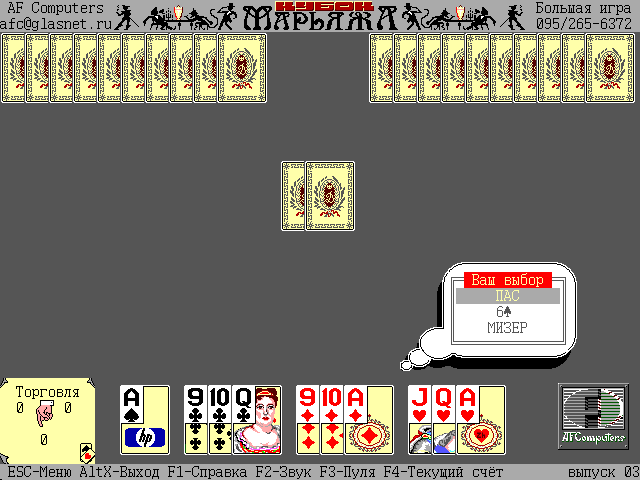
\includegraphics[scale=\FigScale]{examples/marriage/initial_not_patched.png}
\caption{"Торги"}
\end{figure}

Попробуем "подсмотреть" карты в "прикупе" в этой игре.

Для начала --- что мы знаем?
Игра под DOS, датируется 1997-м годом. IDA показывает имена стандартных функций вроде 
\TT{@GetImage\$q7Integert1t1t1m3Any} --- это "манглинг" типичный для Borland Pascal, что позволяет сделать вывод,
что сама игра написана на Паскале и скомпилирована Borland Pascal-ем.

Файлов около 10-и и некоторые имеют текстовую строку в заголовке "Marriage Image Library" --- вероятно,
это библиотеки спрайтов.

В IDA можно увидеть что используется функция \TT{@PutImage\$q7Integert1m3Any4Word}, которая, собственно,
рисует некий спрайт на экране.
Она вызывается по крайней мере из 8-и мест.
Чтобы узнать что происходит в каждом из этих 8-и мест, мы можем блокировать работу каждой функции и смотреть,
что будет происходить.
Например, первая ф-ция имеет адрес seg002:062E, и она заканчивается инструкцией \INS{retf 0Eh} на seg002:102A.
Это означает что метод вызовов ф-ций в Borland Pascal под DOS схож с stdcall --- вызываемая ф-ция должна сама
возвращать стек в состояние до того как началась передача аргументов.
В самом начале этой ф-ции вписываем инструкцию "retf 0eh", либо 3 байта: \TT{CA 0E 00}.
Запускаем "Марьяж" и внешне вроде бы ничего не изменилось.

Переходим ко второй ф-ции, которая активно использует \TT{@PutImage\$q7Integert1m3Any4Word}.
Она находится по адресу seg008:0AB5 и заканчивается инструкцией \INS{retf 0Ah}.
Вписываем эту инструкцию в самом начале и запускаем:

\begin{figure}[H]
\centering
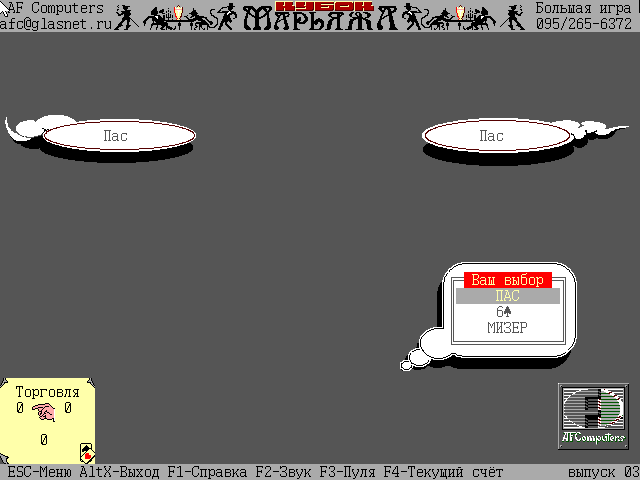
\includegraphics[scale=\FigScale]{examples/marriage/draw_card_bypass.png}
\caption{Карт нет}
\end{figure}

Карт не видно вообще. И видимо, эта функция их отображает, мы её заблокировали, и теперь карт не видно.
Назовем эту ф-цию в IDA \TT{draw\_card()}.
Помимо \TT{@PutImage\$q7Integert1m3Any4Word}, в этой ф-ции вызываются также ф-ции @SetColor\$q4Word, 
\TT{@SetFillStyle\$q4Wordt1}, \TT{@Bar\$q7Integert1t1t1}, \TT{@OutTextXY\$q7Integert16String}.

Сама ф-ция \TT{draw\_cards()} (её название мы дали ей сами только что) вызывается из 4-х мест.
Попробуем точно также "блокировать" каждую ф-цию.

Когда я "блокирую" вторую, по адресу seg008:0DF3 и запускаю программу, вижу такое:

\begin{figure}[H]
\centering
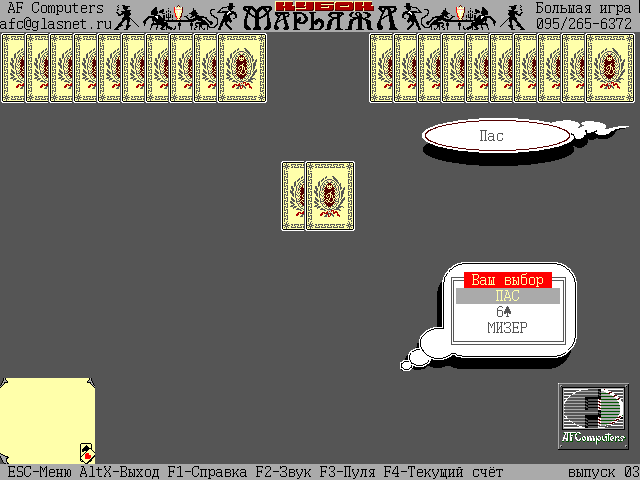
\includegraphics[scale=\FigScale]{examples/marriage/draw_players_cards.png}
\caption{Все карты кроме карт игрока}
\end{figure}

Видны все карты, кроме карт игрока. Видимо, эта функция рисует карты игрока. \\
Я переименовываю её в IDA в \TT{draw\_players\_cards()}.

Четвертая ф-ция, вызывающая \TT{draw\_cards()}, находится по адресу seg008:16B3, и когда я её "блокирую",
я вижу в игре такое:

\begin{figure}[H]
\centering
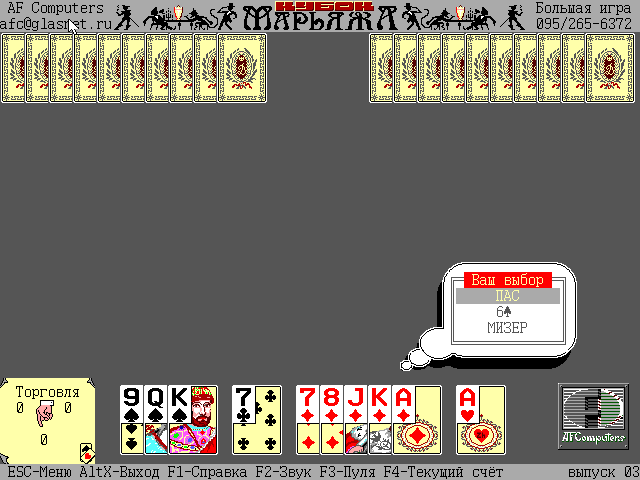
\includegraphics[scale=\FigScale]{examples/marriage/no_prikup.png}
\caption{"Прикупа" нет}
\end{figure}

Все карты есть, кроме "прикупа". Более того, эта ф-ция вызывает только \TT{draw\_cards()}, и только 2 раза.
Видимо эта ф-ция и отображает карты "прикупа".
Будем рассматривать её внимательнее.

\begin{lstlisting}
seg008:16B3 draw_prikup     proc far                ; CODE XREF: seg010:00B0
seg008:16B3                                         ; sub_15098+6
seg008:16B3
seg008:16B3 var_E           = word ptr -0Eh
seg008:16B3 var_C           = word ptr -0Ch
seg008:16B3 arg_0           = byte ptr  6
seg008:16B3
seg008:16B3                 enter   0Eh, 0
seg008:16B7                 mov     al, byte_2C0EA
seg008:16BA                 xor     ah, ah
seg008:16BC                 imul    ax, 23h
seg008:16BF                 mov     [bp+var_C], ax
seg008:16C2                 mov     al, byte_2C0EB
seg008:16C5                 xor     ah, ah
seg008:16C7                 imul    ax, 0Ah
seg008:16CA                 mov     [bp+var_E], ax
seg008:16CD                 cmp     [bp+arg_0], 0
seg008:16D1                 jnz     short loc_1334A
seg008:16D3                 cmp     byte_2BB08, 0
seg008:16D8                 jz      short loc_13356
seg008:16DA
seg008:16DA loc_1334A:                              ; CODE XREF: draw_prikup+1E
seg008:16DA                 mov     al, byte ptr word_32084
seg008:16DD                 mov     byte_293AD, al
seg008:16E0                 mov     al, byte ptr word_32086
seg008:16E3                 mov     byte_293AC, al
seg008:16E6
seg008:16E6 loc_13356:                              ; CODE XREF: draw_prikup+25
seg008:16E6                 mov     al, byte_293AC
seg008:16E9                 xor     ah, ah
seg008:16EB                 push    ax
seg008:16EC                 mov     al, byte_293AD
seg008:16EF                 xor     ah, ah
seg008:16F1                 push    ax
seg008:16F2                 push    [bp+var_C]
seg008:16F5                 push    [bp+var_E]
seg008:16F8                 cmp     [bp+arg_0], 0
seg008:16FC                 jnz     short loc_13379
seg008:16FE                 cmp     byte_2BB08, 0
seg008:1703                 jnz     short loc_13379
seg008:1705                 mov     al, 0
seg008:1707                 jmp     short loc_1337B
seg008:1709 ; ---------------------------------------------------------------------------
seg008:1709
seg008:1709 loc_13379:                              ; CODE XREF: draw_prikup+49
seg008:1709                                         ; draw_prikup+50
seg008:1709                 mov     al, 1
seg008:170B
seg008:170B loc_1337B:                              ; CODE XREF: draw_prikup+54
seg008:170B                 push    ax
seg008:170C                 push    cs
seg008:170D                 call    near ptr draw_card
seg008:1710                 mov     al, byte_2C0EA
seg008:1713                 xor     ah, ah
seg008:1715                 mov     si, ax
seg008:1717                 shl     ax, 1
seg008:1719                 add     ax, si
seg008:171B                 add     ax, [bp+var_C]
seg008:171E                 mov     [bp+var_C], ax
seg008:1721                 cmp     [bp+arg_0], 0
seg008:1725                 jnz     short loc_1339E
seg008:1727                 cmp     byte_2BB08, 0
seg008:172C                 jz      short loc_133AA
seg008:172E
seg008:172E loc_1339E:                              ; CODE XREF: draw_prikup+72
seg008:172E                 mov     al, byte ptr word_32088
seg008:1731                 mov     byte_293AD, al
seg008:1734                 mov     al, byte ptr word_3208A
seg008:1737                 mov     byte_293AC, al
seg008:173A
seg008:173A loc_133AA:                              ; CODE XREF: draw_prikup+79
seg008:173A                 mov     al, byte_293AC
seg008:173D                 xor     ah, ah
seg008:173F                 push    ax
seg008:1740                 mov     al, byte_293AD
seg008:1743                 xor     ah, ah
seg008:1745                 push    ax
seg008:1746                 push    [bp+var_C]
seg008:1749                 push    [bp+var_E]
seg008:174C                 cmp     [bp+arg_0], 0
seg008:1750                 jnz     short loc_133CD
seg008:1752                 cmp     byte_2BB08, 0
seg008:1757                 jnz     short loc_133CD
seg008:1759                 mov     al, 0
seg008:175B                 jmp     short loc_133CF
seg008:175D ; ---------------------------------------------------------------------------
seg008:175D
seg008:175D loc_133CD:                              ; CODE XREF: draw_prikup+9D
seg008:175D                                         ; draw_prikup+A4
seg008:175D                 mov     al, 1
seg008:175F
seg008:175F loc_133CF:                              ; CODE XREF: draw_prikup+A8
seg008:175F                 push    ax
seg008:1760                 push    cs
seg008:1761                 call    near ptr draw_card ; prikup #2
seg008:1764                 leave
seg008:1765                 retf    2
seg008:1765 draw_prikup     endp
\end{lstlisting}

Интересно посмотреть, как именно вызывается \TT{draw\_prikup()}. У нее только один аргумент.

Иногда она вызывается с аргументом 1:

\begin{lstlisting}
...
seg010:084C                 push    1
seg010:084E                 call    draw_prikup
...
\end{lstlisting}

А иногда с аргументом 0, причем вот в таком контексте, где уже есть другая знакомая функция:

\begin{lstlisting}
seg010:0067                 push    1
seg010:0069                 mov     al, byte_31F41
seg010:006C                 push    ax
seg010:006D                 call    sub_12FDC
seg010:0072                 push    1
seg010:0074                 mov     al, byte_31F41
seg010:0077                 push    ax
seg010:0078                 call    draw_players_cards
seg010:007D                 push    2
seg010:007F                 mov     al, byte_31F42
seg010:0082                 push    ax
seg010:0083                 call    sub_12FDC
seg010:0088                 push    2
seg010:008A                 mov     al, byte_31F42
seg010:008D                 push    ax
seg010:008E                 call    draw_players_cards
seg010:0093                 push    3
seg010:0095                 mov     al, byte_31F43
seg010:0098                 push    ax
seg010:0099                 call    sub_12FDC
seg010:009E                 push    3
seg010:00A0                 mov     al, byte_31F43
seg010:00A3                 push    ax
seg010:00A4                 call    draw_players_cards
seg010:00A9                 call    sub_1257A
seg010:00AE                 push    0
seg010:00B0                 call    draw_prikup
seg010:00B5                 mov     byte_2BB95, 0
\end{lstlisting}

Так что единственный аргумент у \TT{draw\_prikup()} может быть или 0 или 1, т.е., это, возможно, булевый тип.
На что он влияет внутри самой ф-ции?
При ближайшем рассмотрении видно, что входящий 0 или 1 передается в \TT{draw\_card()}, т.е., у последней тоже есть
булевый аргумент.
Помимо всего прочего, если передается 1, то по адресам seg008:16DA и seg008:172E копируются несколько байт
из одной группы глобальных переменных в другую.

Эксперимент: здесь 4 раза сравнивается единственный аргумент с 0 и далее следует \INS{JNZ}.
Что если сравнение будет происходит с 1, и, таким образом, работа функции \TT{draw\_prikup()} будет обратной?
Патчим и запускаем:

\begin{figure}[H]
\centering
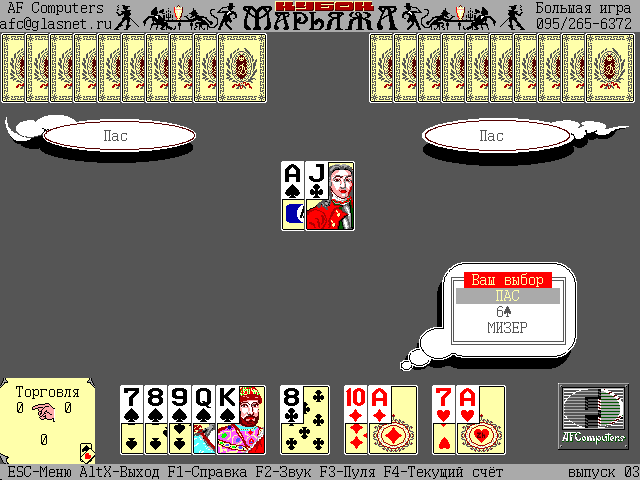
\includegraphics[scale=\FigScale]{examples/marriage/patch1.png}
\caption{"Прикуп" открыт}
\end{figure}

"Прикуп" открыт, но когда я делаю "заказ", и, по логике вещей, "прикуп" теперь должен стать открытым,
он наоборот становится закрытым:

\begin{figure}[H]
\centering
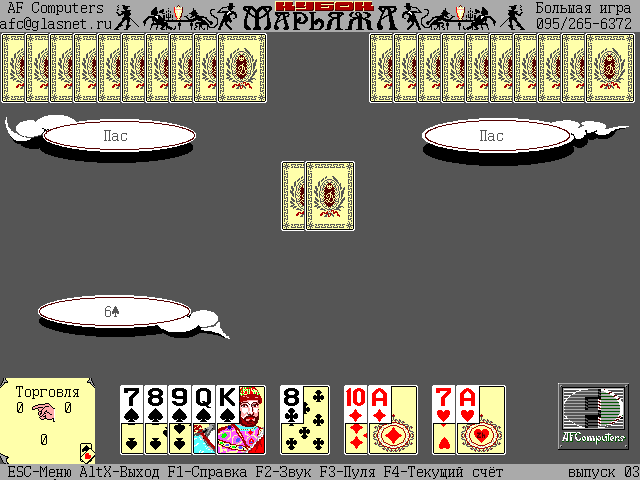
\includegraphics[scale=\FigScale]{examples/marriage/patch2.png}
\caption{"Прикуп" закрыт}
\end{figure}

Всё ясно: если аргумент \TT{draw\_prikup()} нулевой, то карты рисуются рубашкой вверх, если 1, то открытые.
Этот же аргумент передается в \TT{draw\_card()} --- эта ф-ция может рисовать и открытые и закрытые карты.

Пропатчить "Марьяж" теперь легко, достаточно исправить все условные переходы так, как будто бы в ф-цию
всегда приходит 1 в аргументе и тогда "прикуп" всегда будет открыт.

Но что за байты копируются в seg008:16DA и seg008:172E?
Я попробовал забить инструкции копирования \MOV \NOP{}-ами --- "прикуп" вообще перестал отображаться.

Тогда я сделал так, чтобы всегда записывалась 1:

\begin{lstlisting}
...
00004B5A: B001                           mov         al,1
00004B5C: 90                             nop
00004B5D: A26D08                         mov         [0086D],al
00004B60: B001                           mov         al,1
00004B62: 90                             nop
00004B63: A26C08                         mov         [0086C],al
...
\end{lstlisting}

Тогда "прикуп" отображается как два пиковых туза.
А если первый байт --- 2, а второй --- 1, получается трефовый туз.
Видимо так и кодируется масть карты, а затем и сама карта.
% TODO \ref{} сюда о том, как можно передавать аргументы в глоб.переменных
А \TT{draw\_card()} затем считывает эту информацию из пары глобальных переменных.
А копируется она тоже из глобальных переменных, где собственно и находится состояние карт у игроков и в прикупе
после случайной тасовки.
Но нельзя забывать что если мы сделаем так, что в "прикупе" всегда будет 2 пиковых туза, это будет только
на экране так отображаться, а в памяти состояние карт останется таким же, как и после тасовки.

Я также пробовал сделать пранк: во время торгов одна карта "прикупа" открыта, а вторая закрыта, а после "заказа",
наоборот, первая закрыта, а вторая открывается. В качестве упражнения, вы можете попробовать сделать так.

Еще кое-что: чтобы сделать прикуп открытым, ведь можно же найти место где вызывается \TT{draw\_prikup()} и поменять 0
на 1. Можно, только это место не в головой marriage.exe, а в marriage.000, а это DOS-овский оверлей (начинается
с сигнатуры "FBOV").

В качестве упражнения, можно попробовать подсматривать состояние всех карт, и у обоих игроков.
Для этого нужно отладчиком смотреть состояние глобальной памяти рядом с тем, откуда считываются обе карты
прикупа.

Файлы: \\
оригинальная версия: \url{http://beginners.re/examples/marriage/original.zip}, \\
пропатченная мною версия: \url{http://beginners.re/examples/marriage/patched.zip} 
(все 4 условных перехода после \TT{cmp [bp+arg\_0], 0} заменены на \JMP).

}

\section{\EN{Other examples}\RU{Другие примеры}}

\RU{Здесь также был пример с Z3 и ручной декомпиляцией.}
\EN{An example about Z3 and manual decompilation was here.}
\RU{Он (временно) перемещен сюда:}
\EN{It is (temporarily) moved there:}
\url{http://yurichev.com/tmp/SAT_SMT_DRAFT.pdf}.



\chapter{\IFRU{Прочее}{Other things}}

\index{Compiler intrinsic}
\label{compiler_intrinsic}
\section{Compiler intrinsic}

\newcommand{\FNMSDNURL}{\footnote{\url{http://msdn.microsoft.com/en-us/library/5cc576c4.aspx}}}

\index{x86!\Instructions!ROL}
\index{x86!\Instructions!ROR}
\IFRU{Специфичная для компилятора ф-ция не являющяяся обычной библиотечной ф-цией.
Компилятор вместо её вызова генерирует определенный машинный код.
Нередко, это псевдофункции для определенной инструкции \ac{CPU}. \\
\\
Например, в языках \CCpp нет операции циклического сдвига, а во многих \ac{CPU} она есть.
Чтобы программисту были доступны эти инструкции, в MSVC есть псевдофункции 
\IT{\_rotl()} \AndENRU \IT{\_rotr()}\FNMSDNURL{},
которые компилятором напрямую транслируются в x86-инструкции ROL/ROR. \\
\\
Еще один пример это ф-ции позволяющие генерировать SSE-инструкции прямо в коде.}
{A function specific to a compiler which is not usual library function.
Compiler generate a specific machine code instead of call to it.
It is often a pseudofunction for specific \ac{CPU} insruction. \\
\\
For example, there are no cyclic shift operations in \CCpp languages, but present in most \ac{CPU}s.
For programer's convenience, at least MSVC has pseudofunctions
\IT{\_rotl()} \AndENRU \IT{\_rotr()}\FNMSDNURL{}
which are translated by compiler directly to the ROL/ROR x86 instructions. \\
\\
Another example are functions enabling to generate SSE-instructions right in the code.}

\label{anomaly:Intel}
\section{\IFRU{Аномалии компиляторов}{Compiler's anomalies}}
\index{\CompilerAnomaly}
\index{Intel C++}
\index{Oracle RDBMS}
\index{x86!\Instructions!JZ}

\IFRU{Intel C++ 10.1 которым скомпилирован Oracle RDBMS 11.2 Linux86, может сгенерировать два \JZ идущих подряд, 
причем на второй \JZ нет ссылки ниоткуда. Второй \JZ таким образом, не имеет никакого смысла.}
{Intel C++ 10.1, which was used for Oracle RDBMS 11.2 Linux86 compilation, may emit two \JZ in row,
and there are no references to the second \JZ. Second \JZ is thus senseless.}

\begin{lstlisting}[caption=\IFRU{kdli.o из}{kdli.o from} libserver11.a]
.text:08114CF1                   loc_8114CF1:                            ; CODE XREF: __PGOSF539_kdlimemSer+89A
.text:08114CF1                                                           ; __PGOSF539_kdlimemSer+3994
.text:08114CF1 8B 45 08                          mov     eax, [ebp+arg_0]
.text:08114CF4 0F B6 50 14                       movzx   edx, byte ptr [eax+14h]
.text:08114CF8 F6 C2 01                          test    dl, 1
.text:08114CFB 0F 85 17 08 00 00                 jnz     loc_8115518
.text:08114D01 85 C9                             test    ecx, ecx
.text:08114D03 0F 84 8A 00 00 00                 jz      loc_8114D93
.text:08114D09 0F 84 09 08 00 00                 jz      loc_8115518
.text:08114D0F 8B 53 08                          mov     edx, [ebx+8]
.text:08114D12 89 55 FC                          mov     [ebp+var_4], edx
.text:08114D15 31 C0                             xor     eax, eax
.text:08114D17 89 45 F4                          mov     [ebp+var_C], eax
.text:08114D1A 50                                push    eax
.text:08114D1B 52                                push    edx
.text:08114D1C E8 03 54 00 00                    call    len2nbytes
.text:08114D21 83 C4 08                          add     esp, 8
\end{lstlisting}

\begin{lstlisting}[caption=\IFRU{оттуда же}{from the same code}]
.text:0811A2A5                   loc_811A2A5:                            ; CODE XREF: kdliSerLengths+11C
.text:0811A2A5                                                           ; kdliSerLengths+1C1
.text:0811A2A5 8B 7D 08                          mov     edi, [ebp+arg_0]
.text:0811A2A8 8B 7F 10                          mov     edi, [edi+10h]
.text:0811A2AB 0F B6 57 14                       movzx   edx, byte ptr [edi+14h]
.text:0811A2AF F6 C2 01                          test    dl, 1
.text:0811A2B2 75 3E                             jnz     short loc_811A2F2
.text:0811A2B4 83 E0 01                          and     eax, 1
.text:0811A2B7 74 1F                             jz      short loc_811A2D8
.text:0811A2B9 74 37                             jz      short loc_811A2F2
.text:0811A2BB 6A 00                             push    0
.text:0811A2BD FF 71 08                          push    dword ptr [ecx+8]
.text:0811A2C0 E8 5F FE FF FF                    call    len2nbytes
\end{lstlisting}

\IFRU{Возможно, это ошибка его кодегенератора, не выявленная тестами 
(ведь результирующий код и так работает нормально).}
{It is probably code generator bug was not found by tests, because, 
resulting code is working correctly anyway.}

\IFRU{Еще одна такая ошибка компилятора описана здесь}
{Another compiler anomaly I described here}~(\ref{anomaly:LLVM}).

\IFRU{Я показываю здесь подобные случаи для того, чтобы легче было понимать, 
что подобные ошибки компиляторов 
все же имеют место быть, и не следует ломать голову над тем, почему он сгенерировал такой странный код.}
{I demonstrate such cases here, so to understand that such compilers errors are possible and sometimes
one should not to rack one's brain and think why compiler generated such strange code.}

\chapter{\IFRU{Что стоит почитать}{Books/blogs worth reading}}

\section{\IFRU{Книги}{Books}}

\subsection{Windows}

\begin{itemize}
\item
Windows® Internals (Mark E. Russinovich and David A. Solomon with Alex Ionescu)\footnote{\url{http://www.microsoft.com/learning/en/us/book.aspx?ID=12069&locale=en-us}}
\end{itemize}

\subsection{\CCpp}

\begin{itemize}
\item
\IFRU{Стандарт языка Си++}{C++ language standard}: ISO/IEC 14882:2003\footnote{\url{http://www.iso.org/iso/catalogue_detail.htm?csnumber=38110}}
\end{itemize}

\subsection{x86 / x86-64}

\begin{itemize}
\item
\IFRU{Документация от Intel}{Intel manuals}: \url{http://www.intel.com/products/processor/manuals/}
\item
\IFRU{Документация от AMD}{AMD manuals}: \url{http://developer.amd.com/documentation/guides/Pages/default.aspx#manuals}
\end{itemize}

\section{\IFRU{Блоги}{Blogs}}

\subsection{Windows}

\begin{itemize}
\item
\href{http://blogs.msdn.com/oldnewthing/}{Microsoft: Raymond Chen}
\item
\url{http://www.nynaeve.net/}
\end{itemize}


\chapter{\IFRU{Задачи}{Exercises}}

\IFRU{Почти для всех задач, если не указано иное, два вопроса:}
{There are two questions almost for every exercise, if otherwise is not specified:}

1) \IFRU{Что делает эта функция? Ответ должен состоять из одной фразы.}
{What this function does? Answer in one-sentence form.}

2) \IFRU{Перепишите эту функцию на \CCpp}{Rewrite this function into \CCpp}.

\IFRU{Подсказки и ответы собраны в приложении к этой книге.}{Hints and solutions are in the appendix of
this book.}

\section{\IFRU{Легкий уровень}{Easy level}}

\subsection{\Exercise 1.1}

\index{OpenWatcom}
\IFRU{Это стандартная функция из библиотек Си. Исходник взят из OpenWatcom}.
{This is standard C library function. Source code taken from OpenWatcom}.

\subsubsection{MSVC 2010}

\lstinputlisting{exercises/1_1_msvc.asm}

\subsubsection{GCC 4.4.1 + \Othree}

\lstinputlisting{exercises/1_1_gcc.asm}

\subsubsection{Keil (ARM) + \Othree}

\lstinputlisting{exercises/1_1_ARM.s}

\subsubsection{Keil (thumb) + \Othree}

\lstinputlisting{exercises/1_1_thumb.s}

\subsection{\Exercise 1.2}

\index{OpenWatcom}
\IFRU{Это также стандартная функция из библиотек Си. Исходник взят из OpenWatcom и немного переделан}. 
{This is also standard C library function. Source code is taken from OpenWatcom and modified slightly}.

\IFRU{Эта функция использует стандартные функции Си:}
{This function also use these standard C functions:} isspace() \AndENRU isdigit().

\subsubsection{MSVC 2010 + \Ox}

\lstinputlisting{exercises/1_2_msvc.asm}

\subsubsection{GCC 4.4.1}

\IFRU{Задача немного усложняется тем, что GCC представил isspace() и isdigit() 
как inline-функции и вставил их тела прямо в код.}
{This exercise is slightly harder since GCC compiled isspace() and isdigit()
functions as inline-functions and inserted their bodies right into the code.}

\lstinputlisting{exercises/1_2_gcc.asm}

\subsubsection{Keil (ARM) + \Othree}

\lstinputlisting{exercises/1_2_ARM.s}

\subsubsection{Keil (thumb) + \Othree}

\lstinputlisting{exercises/1_2_thumb.s}

\subsection{\Exercise 1.3}

\IFRU{Это также стандартная функция из библиотек Си, а вернее, две функции, работающие в паре. 
Исходник взят из MSVC 2010 и немного переделан.}
{This is standard C function too, actually, two functions working in pair.
Source code taken from MSVC 2010 and modified slightly.}

\IFRU{Суть переделки в том, что эта функция может корректно работать в мульти-тредовой среде, 
а я, для упрощения (или запутывания) убрал поддержку этого.}
{The matter of modification is that this function can work properly in multi-threaded environment,
and I removed its support for simplification (or for confusion).}

\subsubsection{MSVC 2010 + \Ox}

\lstinputlisting{exercises/1_3_msvc.asm}

\subsubsection{GCC 4.4.1}

\lstinputlisting{exercises/1_3_gcc.asm}

\subsubsection{Keil (ARM) + \Othree}

\lstinputlisting{exercises/1_3_ARM.s}

\subsubsection{Keil (thumb) + \Othree}

\lstinputlisting{exercises/1_3_thumb.s}

\subsection{\Exercise 1.4}

\IFRU{Это стандартная функция из библиотек Си. Исходник взят из MSVC 2010.}
{This is standard C library function. Source code taken from MSVC 2010.}

\subsubsection{MSVC 2010 + \Ox}

\lstinputlisting{exercises/1_4_msvc.asm}

\subsubsection{GCC 4.4.1}

\lstinputlisting{exercises/1_4_gcc.asm}

\subsubsection{Keil (ARM) + \Othree}

\lstinputlisting{exercises/1_4_ARM.s}

\subsubsection{Keil (thumb) + \Othree}

\lstinputlisting{exercises/1_4_thumb.s}

\subsection{\Exercise 1.5}

\IFRU{Задача, скорее, на эрудицию, нежели на чтение кода.}
{This exercise is rather on knowledge than on reading code.}

\index{OpenWatcom}
\IFRU{Функция взята из OpenWatcom}.
{The function is taken from OpenWatcom}.

\subsubsection{MSVC 2010 + \Ox}

\lstinputlisting{exercises/1_5_msvc.asm}

\subsection{\Exercise 1.6}

\subsubsection{MSVC 2010 + \Ox}

\lstinputlisting{exercises/1_6_msvc.asm}

\subsubsection{Keil (ARM) + \Othree}

\lstinputlisting{exercises/1_6_ARM.s}

\subsubsection{Keil (thumb) + \Othree}

\lstinputlisting{exercises/1_6_thumb.s}

\subsection{\Exercise 1.7}

\IFRU{Это взята функция из ядра Linux 2.6.}{This function is taken from Linux 2.6 kernel.}

\subsubsection{MSVC 2010 + \Ox}

\lstinputlisting{exercises/1_7_msvc.asm}

\subsubsection{Keil (ARM) + \Othree}

\lstinputlisting{exercises/1_7_ARM.s}

\subsubsection{Keil (thumb) + \Othree}

\lstinputlisting{exercises/1_7_thumb.s}

\subsection{\Exercise 1.8}

\subsubsection{MSVC 2010 + \TT{/O1}}

(/O1: \IFRU{оптимизация по размеру кода}{minimize space}).

\lstinputlisting{exercises/1_8_msvc.asm}

\subsubsection{Keil (ARM) + \Othree}

\lstinputlisting{exercises/1_8_ARM.s}

\subsubsection{Keil (thumb) + \Othree}

\lstinputlisting{exercises/1_8_thumb.s}

\subsection{\Exercise 1.9}

\subsubsection{MSVC 2010 + \TT{/O1}}

(/O1: \IFRU{оптимизация по размеру кода}{minimize space}).

\lstinputlisting{exercises/1_9_msvc.asm}

\subsubsection{Keil (ARM) + \Othree}

\lstinputlisting{exercises/1_9_ARM.s}

\subsubsection{Keil (thumb) + \Othree}

\lstinputlisting{exercises/1_9_thumb.s}

\subsection{\Exercise 1.10}

\IFRU{Если это скомпилировать и запустить, появится некоторое число. Откуда оно берется? 
Откуда оно берется если скомпилировать в MSVC с оптимизациями (\Ox)?}
{If to compile this piece of code and run, a number will be printed. Where it came from?
Where it came from if to compile it in MSVC with optimization (\Ox)?}

\begin{lstlisting}
#include <stdio.h>

int main()
{
	printf ("%d\n");

	return 0;
};
\end{lstlisting}

\subsection{\Exercise 1.11}

% to be proofreaded (begin)
\IFRU{В рамках шутки, ``обманите'' ваш Windows Task Manager чтобы он показывал
больше процессоров/ядер процессоров чем есть в вашем компьютере на самом деле}
{As a practical joke, ``fool'' your Windows Task Manager 
to show much more CPUs/CPU cores than your machine actually has}:

\begin{figure}[H]
\centering
\includegraphics[scale=0.66]{exercises/taskmgr_64cpu_crop.png}
\caption{\IFRU{Обманутый}{Fooled} Windows Task Manager}
\end{figure}
% to be proofreaded (end)

\section{\IFRU{Средний уровень}{Middle level}}

\subsection{\Exercise 2.1}

\IFRU{Довольно известный алгоритм, также включен в стандартную библиотеку Си. Исходник взят из glibc 2.11.1. 
Скомпилирован в GCC 4.4.1 с ключом \TT{-Os} (оптимизация по размеру кода). 
Листинг сделан дизассемблером IDA 4.9 из ELF-файла созданным GCC и линкером.}
{Well-known algorithm, also included in standard C library. Source code was taken from glibc 2.11.1.
Compiled in GCC 4.4.1 with \TT{-Os} option (code size optimization).
Listing was done by IDA 4.9 disassembler from ELF-file generated by GCC and linker.}

\IFRU{Для тех кто хочет использовать IDA в процессе изучения, вот здесь лежат .elf и .idb файлы, 
.idb можно открыть при помощи бесплатной IDA 4.9:}
{For those who wants use IDA while learning, here you may find .elf and .idb files,
.idb can be opened with freeware IDA 4.9:}

\url{http://yurichev.com/RE-exercises/middle/1/}

\lstinputlisting{exercises/2_1_gcc.asm}

\subsection{\Exercise 2.2}

\IFRU{Имеется небольшой исполняемый файл, внутри которого находится довольно известная криптосистема}
{There is a small executable file with a well-known cryptosystem inside}.
\IFRU{Попробуйте её идентифицировать}{Try to identify it}.

\begin{itemize}
\item
\href{http://yurichev.com/RE-exercises/middle/2/unknown_cryptosystem.exe}{Windows x86}

\item
\href{http://yurichev.com/RE-exercises/middle/2/unknown_encryption_linux86.tar}{Linux x86}

\item
\href{http://yurichev.com/RE-exercises/middle/2/unknown_encryption_MacOSX.tar}{MacOSX (x64)}
\end{itemize}

\subsection{\Exercise 2.3}

\IFRU{Имеется небольшой исполняемый файл, некая утилита}
{There is a small executable file, some utility}.
\IFRU{Она открывает другой файл, читает его, что-то вычисляет и показывает число с плавающей точкой}
{It opens another file, reads it, calculate something and prints a float number}.
\IFRU{Попробуйте разобраться, что она делает}{Try to understand what it do}.

\begin{itemize}
\item
\href{http://yurichev.com/RE-exercises/middle/3/unknown_utility_2_3.exe}{Windows x86}

\item
\href{http://yurichev.com/RE-exercises/middle/3/unknown_utility_2_3_Linux86.tar}{Linux x86}

\item
\href{http://yurichev.com/RE-exercises/middle/3/unknown_utility_2_3_MacOSX.tar}{MacOSX (x64)}
\end{itemize}

\subsection{\Exercise 2.4}

\IFRU{Утилита, шифрующая и дешифрующая файлы, по паролю}
{There is an utility which encrypts/decrypts files, by password}.
\IFRU{Есть зашифрованный текстовый файл, пароль неизвестен}{There is an encrypted text file,
password is unknown}.
\IFRU{Зашифрованный файл ~--- это текст на английском языке}{Encrypted file is a text in English language}.
\IFRU{Утилита использует сравнительно мощный алгоритм шифрования, тем не менее,
он был применен с очень грубой ошибкой. И из-за ошибки расшифровать файл вполне возможно с минимумом затрат}
{The utility uses relatively strong cryptosystem, nevertheless, it was implemented with a serious blunder.
Since the mistake present, it is possible to decrypt the file with a little effort.}.

\IFRU{Попробуйте найти ошибку и расшифровать файл}{Try to find the mistake and decrypt the file}.

\begin{itemize}
\item
\href{http://yurichev.com/RE-exercises/middle/4/amateur_cryptor.exe}{Windows x86}

\item
\href{http://yurichev.com/RE-exercises/middle/4/text_encrypted}{\IFRU{Текстовый файл}{Text file}}
\end{itemize}

\subsection{\Exercise 2.5}

\IFRU{Это имитация защиты от копирования использующей ключевой файл}
{This is software copy protection imitation, which uses key file}.
\IFRU{В ключевом файле имя пользователя и серийный номер}
{The key file contain user (or customer) name and serial number}.

\IFRU{Задачи две}{There are two tasks}:

\begin{itemize}
\item
\IFRU{(Простая) при помощи \tracer либо иного отладчика, 
заставьте эту программу принимать измененный ключевой файл}{(Easy) with the help of \tracer
or any other debugger, force the program to accept changed key file}.

\item
\IFRU{(Средняя) ваша задача заключается в том, чтобы изменить в файле имя пользователя на другое, 
но при этом, модифицировать саму программу нельзя}
{(Medium) your goal is to modify user name to another, however, it is not allowed to patch the program}.
\end{itemize}

\begin{itemize}
\item
\href{http://yurichev.com/RE-exercises/middle/5/super_mega_protection.exe}{Windows x86}

\item
\href{http://yurichev.com/RE-exercises/middle/5/super_mega_protection.tar}{Linux x86}

\item
\href{http://yurichev.com/RE-exercises/middle/5/super_mega_protection_MacOSX.tar}{MacOSX (x64)}

\item
\href{http://yurichev.com/RE-exercises/middle/5/sample.key}{\IFRU{Ключевой файл}{Key file}}
\end{itemize}

\subsection{\Exercise 2.6}

\IFRU{Это очень примитивный игрушечный веб-сервер, поддерживающий только статические файлы, без \ac{CGI}, и т.д}
{Here is a very primitive toy web-server, supporting only static files, without \ac{CGI}, etc}.
\IFRU{В нем сознательно оставлено по крайней мере 4 уязвимости}
{At least 4 vulnerabilities are leaved here intentionally}.
\IFRU{Постарайтесь найти их все и использовать для взлома удаленной машины}
{Try to find them all and exploit them in order for breaking into a remote host}.

\begin{itemize}
\item
\href{http://yurichev.com/RE-exercises/middle/6/webserv_win32.rar}{Windows x86}

\item
\href{http://yurichev.com/RE-exercises/middle/6/webserv_Linux_x86.tar}{Linux x86}

\item
\href{http://yurichev.com/RE-exercises/middle/6/webserv_MacOSX_x64.tar}{MacOSX (x64)}
\end{itemize}

\subsection{\Exercise 2.7}

% to be proofreaded (begin)
\IFRU{При помощи \tracer или любого другого win32-отладчика, найдите скрытые мины во время игры,
в стандартной игре Windows MineSweeper}
{With the help of \tracer or any other win32 debugger, reveal hidden mines in the MineSweeper standard Widnows game
during play}.

\IFRU{Подсказка: в}{Hint:} \cite{trew} \IFRU{имеются некоторые описания внутренностей игры MineSweeper}
{have some insights about MineSweeper's internals}.
% to be proofreaded (end)

\section{crackme / keygenme}

\IFRU{Несколько моих \gls{keygenme}:}
{Couple of my \glspl{keygenme}:}

\url{http://crackmes.de/users/yonkie/}


\chapter{\IFRU{Ответы на задачи}{Exercise solutions}}

\section{\IFRU{Легкий уровень}{Easy level}}

\subsection{\Exercise 1.1}

\index{\CStandardLibrary!toupper()}
\IFRU{Решение}{Solution}: \TT{toupper()}.

\IFRU{Исходник на Си}{C source code}:

\begin{lstlisting}
char toupper ( char c )
{
    if( c >= 'a' && c <= 'z' ) {
        c = c - 'a' + 'A';
    }
    return( c );
}
\end{lstlisting}

\subsection{\Exercise 1.2}

\index{\CStandardLibrary!atoi()}
\IFRU{Ответ}{Solution}: \TT{atoi()}

\IFRU{Исходник на Си}{C source code}:

\begin{lstlisting}
#include <stdio.h>
#include <string.h>
#include <ctype.h>

int atoi ( const *p )  /* convert ASCII string to integer */
{
    int i;
    char s;

    while( isspace ( *p ) )
        ++p;
    s = *p;
    if( s == '+' || s == '-' )
        ++p;
    i = 0;
    while( isdigit(*p) ) {
        i = i * 10 + *p - '0';
        ++p;
    }
    if( s == '-' )
        i = - i;
    return( i );
}
\end{lstlisting}

\subsection{\Exercise 1.3}

\index{\CStandardLibrary!rand()}
\index{\CStandardLibrary!srand()}
\IFRU{Ответ}{Solution}: \TT{srand()} / \TT{rand()}.

\IFRU{Исходник на Си}{C source code}:

\begin{lstlisting}
static unsigned int v;

void srand (unsigned int s)
{
        v = s;
}

int rand ()
{
        return( ((v = v * 214013L
            + 2531011L) >> 16) & 0x7fff );
}
\end{lstlisting}

\subsection{\Exercise 1.4}

\index{\CStandardLibrary!strstr()}
\IFRU{Ответ}{Solution}: \TT{strstr()}.

\IFRU{Исходник на Си}{C source code}:

\begin{lstlisting}
char * strstr (
        const char * str1,
        const char * str2
        )
{
        char *cp = (char *) str1;
        char *s1, *s2;

        if ( !*str2 )
            return((char *)str1);

        while (*cp)
        {
                s1 = cp;
                s2 = (char *) str2;

                while ( *s1 && *s2 && !(*s1-*s2) )
                        s1++, s2++;

                if (!*s2)
                        return(cp);

                cp++;
        }

        return(NULL);

}
\end{lstlisting}

\subsection{\Exercise 1.5}

\IFRU{Подсказка}{Hint} \#1: \IFRU{Не забывайте что}{Keep in mind that} 
\TT{\_\_v}\EMDASH\IFRU{глобальная переменная}{global variable}.

\IFRU{Подсказка}{Hint} \#2: \IFRU{Эта функция вызывается startup-кодом перед вызовом \main}
{The function is called in \ac{CRT} startup code, before \main execution}.

\index{x86!\Instructions!FDIV}
\IFRU{Ответ: это проверка на наличие FDIV-ошибки в ранних процессорах Pentium}
{Solution: early Pentium CPU FDIV bug checking}\footnote{\url{http://en.wikipedia.org/wiki/Pentium_FDIV_bug}}.

\IFRU{Исходник на Си}{C source code}:

\begin{lstlisting}
unsigned _v; // _v

enum e {
    PROB_P5_DIV = 0x0001
};

void f( void ) // __verify_pentium_fdiv_bug
{
    /*
        Verify we have got the Pentium FDIV problem.
        The volatiles are to scare the optimizer away.
    */
    volatile double     v1     = 4195835;
    volatile double     v2   = 3145727;

    if( (v1 - (v1/v2)*v2) > 1.0e-8 ) {
        _v |= PROB_P5_DIV;
    }
}
\end{lstlisting}

\subsection{\Exercise 1.6}

\IFRU{Подсказка: если погуглить применяемую здесь константу, это может помочь.}
{Hint: it might be helpful to google a constant used here.}

\IFRU{Ответ: шифрование алгоритмом \ac{TEA}}{Solution: \ac{TEA} encryption algorithm}.

\IFRU{Исходник на Си}{C source code} (\IFRU{взято с}{taken from} \url{http://en.wikipedia.org/wiki/Tiny_Encryption_Algorithm}):

\begin{lstlisting}
void f (unsigned int* v, unsigned int* k) {
    unsigned int v0=v[0], v1=v[1], sum=0, i;           /* set up */
    unsigned int delta=0x9e3779b9;                     /* a key schedule constant */
    unsigned int k0=k[0], k1=k[1], k2=k[2], k3=k[3];   /* cache key */
    for (i=0; i < 32; i++) {                       /* basic cycle start */
        sum += delta;
        v0 += ((v1<<4) + k0) ^ (v1 + sum) ^ ((v1>>5) + k1);
        v1 += ((v0<<4) + k2) ^ (v0 + sum) ^ ((v0>>5) + k3);  
    }                                              /* end cycle */
    v[0]=v0; v[1]=v1;
}
\end{lstlisting}

\subsection{\Exercise 1.7}

\IFRU{Подсказка: таблица содержит заранее вычисленные значения. 
Можно было бы обойтись и без нее, но тогда функция работала бы чуть медленнее.}
{Hint: the table contain pre-calculated values.
It is possible to implement the function without it, but it will work slower, though.}

\IFRU{Ответ: эта функция переставляет все биты во входном 32-битном слове наоборот. 
Это \TT{lib/bitrev.c} из ядра Linux.}
{Solution: this function reverse all bits in input 32-bit integer. 
It is \TT{lib/bitrev.c} from Linux kernel.}

\IFRU{Исходник на Си}{C source code}:

\begin{lstlisting}
const unsigned char byte_rev_table[256] = {
	0x00, 0x80, 0x40, 0xc0, 0x20, 0xa0, 0x60, 0xe0,
	0x10, 0x90, 0x50, 0xd0, 0x30, 0xb0, 0x70, 0xf0,
	0x08, 0x88, 0x48, 0xc8, 0x28, 0xa8, 0x68, 0xe8,
	0x18, 0x98, 0x58, 0xd8, 0x38, 0xb8, 0x78, 0xf8,
	0x04, 0x84, 0x44, 0xc4, 0x24, 0xa4, 0x64, 0xe4,
	0x14, 0x94, 0x54, 0xd4, 0x34, 0xb4, 0x74, 0xf4,
	0x0c, 0x8c, 0x4c, 0xcc, 0x2c, 0xac, 0x6c, 0xec,
	0x1c, 0x9c, 0x5c, 0xdc, 0x3c, 0xbc, 0x7c, 0xfc,
	0x02, 0x82, 0x42, 0xc2, 0x22, 0xa2, 0x62, 0xe2,
	0x12, 0x92, 0x52, 0xd2, 0x32, 0xb2, 0x72, 0xf2,
	0x0a, 0x8a, 0x4a, 0xca, 0x2a, 0xaa, 0x6a, 0xea,
	0x1a, 0x9a, 0x5a, 0xda, 0x3a, 0xba, 0x7a, 0xfa,
	0x06, 0x86, 0x46, 0xc6, 0x26, 0xa6, 0x66, 0xe6,
	0x16, 0x96, 0x56, 0xd6, 0x36, 0xb6, 0x76, 0xf6,
	0x0e, 0x8e, 0x4e, 0xce, 0x2e, 0xae, 0x6e, 0xee,
	0x1e, 0x9e, 0x5e, 0xde, 0x3e, 0xbe, 0x7e, 0xfe,
	0x01, 0x81, 0x41, 0xc1, 0x21, 0xa1, 0x61, 0xe1,
	0x11, 0x91, 0x51, 0xd1, 0x31, 0xb1, 0x71, 0xf1,
	0x09, 0x89, 0x49, 0xc9, 0x29, 0xa9, 0x69, 0xe9,
	0x19, 0x99, 0x59, 0xd9, 0x39, 0xb9, 0x79, 0xf9,
	0x05, 0x85, 0x45, 0xc5, 0x25, 0xa5, 0x65, 0xe5,
	0x15, 0x95, 0x55, 0xd5, 0x35, 0xb5, 0x75, 0xf5,
	0x0d, 0x8d, 0x4d, 0xcd, 0x2d, 0xad, 0x6d, 0xed,
	0x1d, 0x9d, 0x5d, 0xdd, 0x3d, 0xbd, 0x7d, 0xfd,
	0x03, 0x83, 0x43, 0xc3, 0x23, 0xa3, 0x63, 0xe3,
	0x13, 0x93, 0x53, 0xd3, 0x33, 0xb3, 0x73, 0xf3,
	0x0b, 0x8b, 0x4b, 0xcb, 0x2b, 0xab, 0x6b, 0xeb,
	0x1b, 0x9b, 0x5b, 0xdb, 0x3b, 0xbb, 0x7b, 0xfb,
	0x07, 0x87, 0x47, 0xc7, 0x27, 0xa7, 0x67, 0xe7,
	0x17, 0x97, 0x57, 0xd7, 0x37, 0xb7, 0x77, 0xf7,
	0x0f, 0x8f, 0x4f, 0xcf, 0x2f, 0xaf, 0x6f, 0xef,
	0x1f, 0x9f, 0x5f, 0xdf, 0x3f, 0xbf, 0x7f, 0xff,
};

unsigned char bitrev8(unsigned char byte)
{
	return byte_rev_table[byte];
}

unsigned short bitrev16(unsigned short x)
{
	return (bitrev8(x & 0xff) << 8) | bitrev8(x >> 8);
}

/**
 * bitrev32 - reverse the order of bits in a unsigned int value
 * @x: value to be bit-reversed
 */

unsigned int bitrev32(unsigned int x)
{
	return (bitrev16(x & 0xffff) << 16) | bitrev16(x >> 16);
}
\end{lstlisting}

\subsection{\Exercise 1.8}

\IFRU{Ответ: сложение двух матриц размером 100 на 200 элементов типа \Tdouble.}
{Solution: two 100*200 matrices of \Tdouble type addition.}

\IFRU{Исходник на \CCpp}{\CCpp source code}:

\begin{lstlisting}
#define M    100
#define N    200

void s(double *a, double *b, double *c)
{
  for(int i=0;i<N;i++)
    for(int j=0;j<M;j++)
      *(c+i*M+j)=*(a+i*M+j) + *(b+i*M+j);
};
\end{lstlisting}

\subsection{\Exercise 1.9}

\IFRU{Ответ: умножение двух матриц размерами 100*200 и 100*300 элементов типа \Tdouble, результат: матрица 100*300.}
{Solution: two matrices (one is 100*200, second is 100*300) of \Tdouble type multiplication, result: 100*300
matrix.}

\IFRU{Исходник на \CCpp}{\CCpp source code}:

\begin{lstlisting}
#define M     100
#define N     200
#define P     300

void m(double *a, double *b, double *c)
{
  for(int i=0;i<M;i++)
    for(int j=0;j<P;j++)
    {
      *(c+i*M+j)=0;
      for (int k=0;k<N;k++) *(c+i*M+j)+=*(a+i*M+j) * *(b+i*M+j);
    }
};
\end{lstlisting}

\subsection{\Exercise 1.11}

% to be proofreaded (begin)
\IFRU{Подсказка: Task Manager узнает количество процессоров/ядер используя вызов ф-ции
\TT{NtQuerySystemInformation(SystemBasicInformation, ..., ..., ...)}, этот вызов можно найти и подставлять
туда другое значение.}
{Hint: Task Manager get CPU/CPU cores count using function call 
\TT{NtQuerySystemInformation(SystemBasicInformation, ..., ..., ...)}, it is possible to find that
call and to substitute resulting number.}

\IFRU{И разумеется, Task Manager будет показывать некорректные результаты в графиках 
истории загрузки процессоров/ядер}{And of course, 
the Task Manager will show incorrect results in CPU usage history}.
% to be proofreaded (end)

\section{\IFRU{Средний уровень}{Middle level}}

\subsection{\Exercise 2.1}

\IFRU{Подсказка \#1: В этом коде есть одна особенность, по которой можно значительно сузить поиск функции в glibc.}
{Hint \#1: The code has one characteristic thing, if considering it, it may help narrowing search of right function 
among glibc functions}.

\IFRU{Ответ: особенность ~--- это вызов callback-функции}{Solution: characteristic~---is callback-function
calling}~(\ref{sec:pointerstofunctions}),
\IFRU{указатель на которую передается в четвертом аргументе}{pointer to which is passed in 4th
argument}. \IFRU{Это}{It is} \TT{quicksort()}.

\index{\CStandardLibrary!qsort()}
\href{http://yurichev.com/RE-exercise-solutions/middle/1/2_1.c}{\IFRU{Исходник на Си}{C source code}}.

\subsection{\Exercise 2.2}

\IFRU{Подсказка: проще всего конечно же искать по значениями в таблицах}
{Hint: easiest way is to find by values in the tables}.

\href{http://yurichev.com/RE-exercise-solutions/middle/2/gost.c}
{\IFRU{Исходник на Си с комментариями}{Commented C source code}}.

\subsection{\Exercise 2.3}

\href{http://yurichev.com/RE-exercise-solutions/middle/3/entropy.c}
{\IFRU{Исходник на Си с комментариями}{Commented C source code}}.

\subsection{\Exercise 2.4}

\href{http://yurichev.com/RE-exercise-solutions/middle/4/}
{\IFRU{Исходник на Си с комментариями, а также расшифрованный файл}{Commented C source code, and also decrypted file}}.

\subsection{\Exercise 2.5}

\IFRU{Подсказка: как видно, строка где указано имя пользователя занимает не весь ключевой файл}
{Hint: as we can see, the string with user name occupies not the whole file}.

\IFRU{Байты за терминирующим нулем вплоть до смещения \TT{0x7F} игнорируются программой}
{Bytes after terminated zero till offset \TT{0x7F} are ignored by program}.

\href{http://yurichev.com/RE-exercise-solutions/middle/5/crc16_keyfile_check.c}
{\IFRU{Исходник на Си с комментариями}{Commented C source code}}.

\subsection{\Exercise 2.6}

\href{http://yurichev.com/RE-exercise-solutions/middle/6/}
{\IFRU{Исходник на Си с комментариями}{Commented C source code}}.

\IFRU{В качестве еще одного упражнения, теперь вы можете попробовать исправить уязвимости в этом веб-сервере}
{As another exercise, now you may try to fix all vulnerabilities you found in this web-server}.


\part*{\RU{Послесловие}\EN{Afterword}}
\addcontentsline{toc}{part}{\RU{Послесловие}\EN{Afterword}}

\chapter{\RU{Вопросы?}\EN{Questions?}}

\RU{Совершенно по любым вопросам вы можете не раздумывая писать автору}%
\EN{Do not hesitate to mail any questions to the author}: \TT{<\EMAIL>}

\EN{Any suggestions what also should be added to my book?}%
\RU{Есть идеи о том, что ещё можно добавить в эту книгу?}
 
\RU{Пожалуйста, присылайте мне информацию о замеченных ошибках (включая грамматические),}
\EN{Please, do not hesitate to send me any corrections (including grammar (you see how horrible my English is?)),}\etc.\\
\\
\RU{Автор много работает над книгой, поэтому номера страниц, листингов, \etc. очень часто меняются.}%
\EN{The author is working on the book a lot, so the page and listing numbers, \etc. are changing very rapidly.}
\RU{Пожалуйста, в своих письмах мне не ссылайтесь на номера страниц и листингов.}%
\EN{Please, do not refer to page and listing numbers in your emails to me.}
\RU{Есть метод проще: сделайте скриншот страницы, затем в графическом редакторе подчеркните место, где вы видите
ошибку, и отправьте автору. Так он может исправить её намного быстрее.}%
\EN{There is a much simpler method: make a screenshot of the page, in a graphics editor underline the place where you see the error,
and send it to me. He'll fix it much faster.}
\RU{Ну а если вы знакомы с git и \LaTeX, вы можете исправить ошибку прямо в исходных текстах:}\EN{And if you familiar with git and \LaTeX\, you can fix the error right in the source code:}\\
\href{http://go.yurichev.com/17089}{GitHub}.\\
\\
\EN{Do not worry to bother me while writing me about any petty mistakes you found, even if you are not very confident.
I'm writing for beginners, after all, so beginners' opinions and comments are crucial for my job.}
\RU{Не бойтесь побеспокоить меня написав мне о какой-то мелкой ошибке, даже если вы не очень уверены.
Я всё-таки пишу для начинающих, поэтому мнение и коментарии именно начинающих очень важны для моей работы.}


\part*{\RU{Приложение}\EN{Appendix}}
\appendix
\addcontentsline{toc}{part}{\RU{Приложение}\EN{Appendix}}

% chapters
\section{x86}

\subsection{\RU{Терминология}\EN{Terminology}}

\RU{Общее для 16-bit (8086/80286), 32-bit (80386, \etc{}.), 64-bit.}
\EN{Common for 16-bit (8086/80286), 32-bit (80386, \etc{}), 64-bit.}

\myindex{IEEE 754}
\myindex{MS-DOS}
\begin{description}
	\item[byte] 8-\bitENRU. 
		\RU{Для определения переменных и массива байт используется директива ассемблера DB}
		\EN{The DB assembly directive is used for defining variables and arrays of bytes}.
		\RU{Байты передаются в 8-битных частях регистров}
		\EN{Bytes are passed in the 8-bit part of registers}: \TT{AL/BL/CL/DL/AH/BH/CH/DH/SIL/DIL/R*L}.
	\item[word] 16-\bitENRU. \RU{\dittoclosing директива ассемблера DW}
		\EN{DW assembly directive \dittoclosing}.
		\RU{Слова передаются в 16-битных частях регистров}\EN{Words are passed in the 16-bit part
		of the registers}: \TT{AX/BX/CX/DX/SI/DI/R*W}.
	\item[double word] (\q{dword}) 32-\bitENRU. \RU{\dittoclosing директива ассемблера DD}
		\EN{DD assembly directive \dittoclosing}.
		\RU{Двойные слова передаются в регистрах}
		\EN{Double words are passed in registers} (x86) \RU{или в 32-битных частях регистров}
		\EN{or in the 32-bit part of registers} (x64). 
		\RU{В 16-битном коде, двойные слова передаются в парах 16-битных регистров}
		\EN{In 16-bit code, double words are passed in 16-bit register pairs}.
	\item[quad word] (\q{qword}) 64-\bitENRU. \RU{\dittoclosing директива ассемблера DQ}
		\EN{DQ assembly directive \dittoclosing}.
		\RU{В 32-битной среде, учетверенные слова передаются в парах 32-битных регистров}
		\EN{In 32-bit environment, quad words are passed in 32-bit register pairs}.
	\EN{\item[tbyte] (10 bytes) 80-bit or 10 bytes (used for IEEE 754 FPU registers).}%
	\RU{\item[tbyte] (10 байт) 80-бит или 10 байт (используется для регистров IEEE 754 FPU).}
	\item[paragraph] (16 \RU{байт}\EN{bytes})\EMDASH{}\RU{термин был популярен в среде MS-DOS}
	\EN{term was popular in MS-DOS environment}.
\end{description}

\myindex{Windows!API}
\RU{Типы данных с той же шириной (BYTE, WORD, DWORD) точно такие же и в}
\EN{Data types of the same width (BYTE, WORD, DWORD) are also the same in} Windows \ac{API}.

\section{\IFRU{Регистры общего пользования}{General purpose registers}}

\IFRU{Ко многим регистрам можно обращаться как к частям размером в байт или 16-битное слово}
{It is possible to access many registers by byte or 16-bit word parts}.
\IFRU{Это всё\EMDASH{}наследие от более старых процессоров Intel (вплоть до 8-битного 8080),
все еще поддерживаемое для обратной совместимости}{It is all inheritance from older Intel CPUs (up to 8-bit 8080) 
still supported for backward compatibility}.
\IFRU{Например, в \ac{RISC} процессорах, такой возможности, как правило, нет}{For example, this feature
is usually not present in \ac{RISC} CPUs}.

\index{x86-64}
\IFRU{Регистры, имеющие префикс R- появились только в x86-64, а префикс E- ~--- в 80386}
{Registers prefixed with R- appeared in x86-84, and those prefixed with E-~---in 80386}.
\IFRU{Таким образом, R-регистры 64-битные, а E-регистры ~--- 32-битные}
{Thus, R-registers are 64-bit, and E-registers~---32-bit}.

\IFRU{В x86-64 добавили еще 8 \ac{GPR}: R8-R15}
{8 more \ac{GPR}'s were added in x86-86: R8-R15}.

N.B.: \IFRU{В документации от Intel, для обращения к самому младшему байту к имени регистра
нужно добавлять суффикс \IT{L}: \IT{R8L}, но \ac{IDA} называет эти регистры добавляя суффикс \IT{B}: \IT{R8B}}
{In the Intel manuals byte parts of these registers are prefixed by \IT{L}, e.g.: \IT{R8L}, but \ac{IDA}
names these registers by adding \IT{B} suffix, e.g.: \IT{R8B}}.

\subsection{RAX/EAX/AX/AL}
\RegTableOne{RAX}{EAX}{AX}{AH}{AL}

\ac{AKA} \IFRU{аккумулятор}{accumulator}.
\IFRU{Результат ф-ции обычно возвращается через этот регистр}
{The result of function if usually returned via this register}.

\subsection{RBX/EBX/BX/BL}
\RegTableOne{RBX}{EBX}{BX}{BH}{BL}

\subsection{RCX/ECX/CX/CL}
\RegTableOne{RCX}{ECX}{CX}{CH}{CL}

\ac{AKA} \IFRU{счетчик}{counter}: 
\IFRU{используется в этой роли в инструкциях с префиксом REP и в инструкциях сдвига}
{in this role it is used in REP prefixed instructions and also in shift instructions}
(SHL/SHR/RxL/RxR).

\subsection{RDX/EDX/DX/DL}
\RegTableOne{RDX}{EDX}{DX}{DH}{DL}

\subsection{RSI/ESI/SI/SIL}
\RegTableTwo{RSI}{ESI}{SI}{SIL}

\ac{AKA} ``source''. \IFRU{Используется как источник в инструкциях}{Used as source in the instructions} 
REP MOVSx, REP CMPSx.

\subsection{RDI/EDI/DI/DIL}
\RegTableTwo{RDI}{EDI}{DI}{DIL}

\ac{AKA} ``destination''. \IFRU{Используется как указатель на место назначения в инструкции}
{Used as a pointer to destination place in the instructions} REP MOVSx, REP STOSx.

\subsection{R8/R8D/R8W/R8L}
\RegTableThree{R8}{R8D}{R8W}{R8L}

\subsection{R9/R9D/R9W/R9L}
\RegTableThree{R9}{R9D}{R9W}{R9L}

\subsection{R10/R10D/R10W/R10L}
\RegTableThree{R10}{R10D}{R10W}{R10L}

\subsection{R11/R11D/R11W/R11L}
\RegTableThree{R11}{R11D}{R11W}{R11L}

\subsection{R12/R12D/R12W/R12L}
\RegTableThree{R12}{R12D}{R12W}{R12L}

\subsection{R13/R13D/R13W/R13L}
\RegTableThree{R13}{R13D}{R13W}{R13L}

\subsection{R14/R14D/R14W/R14L}
\RegTableThree{R14}{R14D}{R14W}{R14L}

\subsection{R15/R15D/R15W/R15L}
\RegTableThree{R15}{R15D}{R15W}{R15L}

\subsection{RSP/ESP/SP/SPL}
\RegTableTwo{RSP}{ESP}{SP}{SPL}

\ac{AKA} \gls{stack pointer}. \IFRU{Обычно всегда указывает на текущий стек, кроме тех случаев,
когда он не инициализирован}{Usually points to the current stack except those cases when it is not yet initialized}.

\subsection{RBP/EBP/BP/BPL}
\RegTableTwo{RBP}{EBP}{BP}{BPL}

\ac{AKA} frame pointer. \IFRU{Обычно используется для доступа к локальным переменным ф-ции и аргументам,
Больше о нем}
{Usually used for local variables and arguments of function accessing. More about it}: (\ref{stack_frame}).

\subsection{RIP/EIP/IP}

\begin{center}
\begin{tabular}{ | l | l | l | l | l | l | l | l | l |}
\hline
\RegHeader \\
\hline
\multicolumn{8}{ | c | }{RIP\textsuperscript{x64}} \\
\hline
\multicolumn{4}{ | c | }{} & \multicolumn{4}{ c | }{EIP} \\
\hline
\multicolumn{6}{ | c | }{} & \multicolumn{2}{ c | }{IP} \\
\hline
\end{tabular}
\end{center}

\ac{AKA} ``instruction pointer''
\footnote{\IFRU{Иногда называется так же}{Sometimes also called} ``program counter''}.
\IFRU{Обычно всегда указывает на исполняющуюся инструкцию}{Usually always points to the current instruction}.
\IFRU{Напрямую модифицировать
регистр нельзя, хотя можно делать так (что равноценно)}
{Cannot be modified, however, it is possible to do (which is equivalent to)}:

\begin{lstlisting}
mov eax...
jmp eax
\end{lstlisting}

\IFRU{Либо}{Or}:

\begin{lstlisting}
push val
ret
\end{lstlisting}

\subsection{CS/DS/ES/SS/FS/GS}

\IFRU{16-битные регистры, содержащие селектор кода}{16-bit registers containing code selector} (CS), 
\IFRU{данных}{data selector} (DS), \IFRU{стека}{stack selector} (SS).\\
\\
\index{TLS}
\index{Windows!TIB}
FS \InENRU win32 \IFRU{указывает на}{points to} \ac{TLS}, \IFRU{а в Linux на эту роль был выбран GS}
{GS took this role in Linux}.
\IFRU{Это сделано для более быстрого доступа к \ac{TLS} и прочим структурам там вроде \ac{TIB}}
{It is done for faster access to the \ac{TLS} and other structures like \ac{TIB}}.
\\
\IFRU{В прошлом эти регистры использовались как сегментные регистры}
{In the past, these registers were used as segment registers} (\ref{8086_memory_model}).

\subsection{\IFRU{Регистр флагов}{Flags register}}

\label{EFLAGS}
\ac{AKA} EFLAGS.

\begin{center}
\begin{tabular}{ | l | l | l | }
\hline
\headercolor{} \IFRU{Бит}{Bit} (\IFRU{маска}{mask}) &
\headercolor{} \IFRU{Аббревиатура}{Abbreviation} (\IFRU{значение}{meaning}) &
\headercolor{} \IFRU{Описание}{Description} \\
\hline
0 (1) & CF (Carry) & \RU{Флаг переноса.} \\
      &            & \IFRU{Инструкции}{The} CLC/STC/CMC \IFRU{используются}{instructions are used} \\
      &            & \IFRU{для установки/сброса/инвертирования этого флага}{for setting/resetting/toggling this flag} \\
\hline
2 (4) & PF (Parity) & \RU{Флаг четности }(\ref{parity_flag}). \\
\hline
4 (0x10) & AF (Adjust) & \\
\hline
6 (0x40) & ZF (Zero) & \IFRU{Выставляется в}{Setting to} 0 \\
         &           & \IFRU{если результат последней операции был}{if the last operation's result was} 0. \\
\hline
7 (0x80) & SF (Sign) & \RU{Флаг знака.} \\
\hline
8 (0x100) & TF (Trap) & \IFRU{Применяется при отладке}{Used for debugging}. \\
&         &             \IFRU{Если включен, то после исполнения каждой инструкции}{If turned on, an exception will be} \\
&         &             \IFRU{будет сгенерировано исключение}{generated after each instruction execution}. \\
\hline
9 (0x200) & IF (Interrupt enable) & \IFRU{Разрешены ли прерывания}{Are interrupts enabled}. \\
          &                       & \IFRU{Инструкции}{The} CLI/STI \IFRU{используются}{instructions are used} \\
	  &                       & \IFRU{для установки/сброса этого флага}{for the flag setting/resetting} \\
\hline
10 (0x400) & DF (Direction) & \IFRU{Задается направление для инструкций}{A directions is set for the} \\
           &                & REP MOVSx, REP CMPSx, REP LODSx, REP SCASx\EN{ instructions}.\\
           &                & \IFRU{Инструкции}{The} CLD/STD \IFRU{используются}{instructions are used} \\
	   &                & \IFRU{для установки/сброса этого флага}{for the flag setting/resetting} \\
\hline
11 (0x800) & OF (Overflow) & \RU{Переполнение.} \\
\hline
12, 13 (0x3000) & IOPL (I/O privilege level)\textsuperscript{80286} & \\
\hline
14 (0x4000) & NT (Nested task)\textsuperscript{80286} & \\
\hline
16 (0x10000) & RF (Resume)\textsuperscript{80386} & \IFRU{Применяется при отладке}{Used for debugging}. \\
             &                  & \IFRU{Если включить,}{CPU will ignore hardware breakpoint in DRx} \\
	     &                  & \IFRU{CPU проигнорирует хардварную точку останова в DRx}{if the flag is set}. \\
\hline
17 (0x20000) & VM (Virtual 8086 mode)\textsuperscript{80386} & \\
\hline
18 (0x40000) & AC (Alignment check)\textsuperscript{80486} & \\
\hline
19 (0x80000) & VIF (Virtual interrupt)\textsuperscript{Pentium} & \\
\hline
20 (0x100000) & VIP (Virtual interrupt pending)\textsuperscript{Pentium} & \\
\hline
21 (0x200000) & ID (Identification)\textsuperscript{Pentium} & \\
\hline
\end{tabular}
\end{center}

\IFRU{Остальные флаги зарезервированы}{All the rest flags are reserved}.

\section{FPU-\IFRU{регистры}{registers}}

\index{x86!FPU}
8 80-\IFRU{битных регистров работающих как стек}{bit registers working as a stack}: ST(0)-ST(7).
N.B.: \ac{IDA} \IFRU{называет}{calls} ST(0) \IFRU{просто}{as just} ST.
\IFRU{Числа хранятся в формате}{Numbers are stored in the} IEEE 754\EN{ format}.

\IFRU{Формат значения \IT{long double}}{\IT{long double} value format}:

\bigskip
% a hack used here! http://tex.stackexchange.com/questions/73524/bytefield-package
\begin{center}
\begingroup
\makeatletter
\let\saved@bf@bitformatting\bf@bitformatting
\renewcommand*{\bf@bitformatting}{%
	\ifnum\value{header@val}=21 %
	\value{header@val}=62 %
	\else\ifnum\value{header@val}=22 %
	\value{header@val}=63 %
	\else\ifnum\value{header@val}=23 %
	\value{header@val}=64 %
	\else\ifnum\value{header@val}=30 %
	\value{header@val}=78 %
	\else\ifnum\value{header@val}=31 %
	\value{header@val}=79 %
	\fi\fi\fi\fi\fi
	\saved@bf@bitformatting
}%
\begin{bytefield}{32}
	\bitheader[endianness=big]{0,21,22,23,30,31} \\
	\bitbox{1}{S} &
	\bitbox{8}{\IFRU{экспонента}{exponent}} &
	\bitbox{1}{I} &
	\bitbox{22}{\IFRU{мантисса}{mantissa or fraction}}
\end{bytefield}
\endgroup
\end{center}

\begin{center}
( S\EMDASH{}\IFRU{знак}{sign}, I\EMDASH{}\IFRU{целочисленная часть}{integer part} )
\end{center}

\label{FPU_control_word}
\subsection{\IFRU{Регистр управления}{Control Word}}

\IFRU{Регистр, при помощи которого можно задавать поведение}{Register controlling behaviour of the}
\ac{FPU}.

\begin{center}
\begin{tabular}{ | l | l | l | }
\hline
\IFRU{Бит}{Bit} &
\IFRU{Аббревиатура (значение)}{Abbreviation (meaning)} &
\IFRU{Описание}{Description} \\
\hline
0   & IM (Invalid operation Mask) & \\
\hline
1   & DM (Denormalized operand Mask) & \\
\hline
2   & ZM (Zero divide Mask) & \\
\hline
3   & OM (Overflow Mask) & \\
\hline
4   & UM (Underflow Mask) & \\
\hline
5   & PM (Precision Mask) & \\
\hline
7   & IEM (Interrupt Enable Mask) & \IFRU{Разрешение исключений, по умолчанию 1 (запрещено)}
{Exceptions enabling, 1 by default (disabled)} \\
\hline
8, 9 & PC (Precision Control) & \RU{Управление точностью} \\
     &                        & 00 ~--- 24 \IFRU{бита}{bits} (REAL4) \\
     &                        & 10 ~--- 53 \IFRU{бита}{bits} (REAL8) \\
     &                        & 11 ~--- 64 \IFRU{бита}{bits} (REAL10) \\
\hline
10, 11 & RC (Rounding Control) & \RU{Управление округлением} \\
       &                       & 00 ~--- \IFRU{(по умолчанию) округлять к ближайшему}{(by default) round to nearest} \\
       &                       & 01 ~--- \IFRU{округлять к}{round toward} $-\infty$ \\
       &                       & 10 ~--- \IFRU{округлять к}{round toward} $+\infty$ \\
       &                       & 11 ~--- \IFRU{округлять к}{round toward} $0$ \\
\hline
12 & IC (Infinity Control) & 0 ~--- (\IFRU{по умолчанию}{by default}) \IFRU{считать}{treat} $+\infty$ \AndENRU $-\infty$ \IFRU{за беззнаковое}{as unsigned} \\
   &                       & 1 ~--- \IFRU{учитывать и}{respect both} $+\infty$ \AndENRU $-\infty$ \\
\hline
\end{tabular}
\end{center}

\IFRU{Флагами}{The} PM, UM, OM, ZM, DM, IM 
\IFRU{задается, генерировать ли исключения в случае соответствующих ошибок}
{flags are defining if to generate exception in case of corresponding errors}.

\subsection{\IFRU{Регистр статуса}{Status Word}}

\label{FPU_status_word}
\IFRU{Регистр только для чтения}{Read-only register}.

\begin{center}
\begin{tabular}{ | l | l | l | }
\hline
\IFRU{Бит}{Bit} &
\IFRU{Аббревиатура (значение)}{Abbreviation (meaning)} &
\IFRU{Описание}{Description} \\
\hline
15   & B (Busy) & \IFRU{Работает ли сейчас FPU}{Is FPU do something} (1)
\IFRU{или закончил и результаты готовы}{or results are ready} (0) \\
\hline
14   & C3 & \\
\hline
13, 12, 11 & TOP & \IFRU{указывает, какой сейчас регистр является нулевым}
{points to the currently zeroth register} \\
\hline
10 & C2 & \\
\hline
9  & C1 & \\
\hline
8  & C0 & \\
\hline
7  & IR (Interrupt Request) & \\
\hline
6  & SF (Stack Fault) & \\
\hline
5  & P (Precision) & \\
\hline
4  & U (Underflow) & \\
\hline
3  & O (Overflow) & \\
\hline
2  & Z (Zero) & \\
\hline
1  & D (Denormalized) & \\
\hline
0  & I (Invalid operation) & \\
\hline
\end{tabular}
\end{center}

\IFRU{Биты}{The} SF, P, U, O, Z, D, I \IFRU{сигнализируют об исключениях}
{bits are signaling about exceptions}.

\IFRU{О}{About the} C3, C2, C1, C0 \IFRU{читайте больше}{read more}: (\ref{Czero_etc}).

N.B.: \IFRU{когда используется регистр ST(x), FPU прибавляет $x$ к TOP по модулю 8 и получается номер
внутреннего регистра}{When ST(x) is used, FPU adds $x$ to TOP (by modulo 8) and that is how it gets 
internal register's number}.

\subsection{Tag Word}

\IFRU{Этот регистр отражает текущее содержимое регистров чисел}
{The register has current information about number's registers usage}.

\begin{center}
\begin{tabular}{ | l | l | l | }
\hline
\IFRU{Бит}{Bit} & \IFRU{Аббревиатура (значение)}{Abbreviation (meaning)} \\
\hline
15, 14 & Tag(7) \\
\hline
13, 12 & Tag(6) \\
\hline
11, 10 & Tag(5) \\
\hline
9, 8 & Tag(4) \\
\hline
7, 6 & Tag(3) \\
\hline
5, 4 & Tag(2) \\
\hline
3, 2 & Tag(1) \\
\hline
1, 0 & Tag(0) \\
\hline
\end{tabular}
\end{center}

\IFRU{Для каждого тэга}{For each tag}:

\begin{itemize}
\item
00 ~--- \IFRU{Регистр содержит ненулевое значение}{The register contains a non-zero value}
\item
01 ~--- \IFRU{Регистр содержит 0}{The register contains 0}
\item
10 ~--- \IFRU{Регистр содержит специальное число}{The register contains a special value} 
(\ac{NAN}, $\infty$, \OrENRU \IFRU{денормализованное число}{denormal})
\item
11 ~--- \IFRU{Регистр пуст}{The register is empty}
\end{itemize}

\section{SIMD-\IFRU{регистры}{registers}}

\subsection{MMX-\IFRU{регистры}{registers}}

8 64-\IFRU{битных регистров}{bit registers}: MM0..MM7.

\subsection{SSE \AndENRU AVX-\IFRU{регистры}{registers}}

\index{x86-64}
SSE: 8 128-\IFRU{битных регистров}{bit registers}: XMM0..XMM7.
\IFRU{В}{In the} x86-64 \IFRU{добавлено еще 8 регистров}{8 more registers were added}: XMM8..XMM15.

AVX \IFRU{это расширение всех регистры до 256 бит}{is the extension of all these registers to 256 bits}.

\input{appendix/x86/DRx}

% TODO: control registers
 % subsection
% to be proofreaded
\subsection{\IFRU{Инструкции}{Instructions}}

\IFRU{Инструкции отмеченные как (M) обычно не генерируются компилятором: если вы видите её, вероятно,
это вручную написанный фрагмент кода, либо это т.н. compiler intrinsic}
{Instructions marked as (M) are not usually generated by compiler: if you see it, it is probably
hand-written piece of assembly code, or this is compiler intrinsic} (\ref{compiler_intrinsic}).

% TODO ? обратные инструкции

\IFRU{Только наиболее используемые инструкции перечислены здесь}
{Only most frequently used instructions are listed here}.
\IFRU{Обращайтесь к}{Read} \cite{Intel} \OrENRU \cite{AMD} 
\IFRU{для полной документации}{for a full documentation}.

\subsubsection{\IFRU{Префиксы}{Prefixes}}

\begin{description}
\label{x86_lock}
\item[LOCK] \IFRU{используется чтобы предоставить эксклюзивный доступ к памяти в многопроцессорной среде}
{force CPU to make exclusive access to the RAM in multiprocessor environment}.
\IFRU{Для упрощения, можно сказать, что когда исполняется инструкция с этим префиксом, остальные процессоры
в системе останавливаются}{For the sake of simplification, it can be said that when instruction
with this prefix is executed, all other CPUs in multiprocessor system is stopped}.
\IFRU{Чаще все это используется для критических секций, семафоров, мьютексов}{Most often
it is used for critical sections, semaphores, mutexes}.
\IFRU{Обычно используется с}{Commonly used with} ADD, AND, BTR, BTS, CMPXCHG, OR, XADD, XOR.
\IFRU{Читайте больше о критических секциях}{Read more about critical sections} (\ref{critical_sections}).

\item[REP] \IFRU{используется с инструкциями}{used with} MOVSx \AndENRU STOSx\IFRU{ instructions}{}:
\IFRU{инструкция будет исполняться в цикле, счетчик расположен в регистре CX/ECX/RCX}
{execute the instruction in loop, counter is located in the CX/ECX/RCX register}.
\IFRU{Для более детального описания, читайте больше об инструкциях}
{For detailed description, read more about} MOVSx (\ref{REP_MOVSx}) 
\AndENRU STOSx (\ref{REP_STOSx})\IFRU{}{ instructions}.

\IFRU{Работа инструкций с префиксом REP зависит от флага DF, он задает направление}
{Instructions prefixed by REP are sensitive to DF flag, which is used to set direction}.

\item[REPE/REPNE] (\ac{AKA} REPZ/REPNZ) \IFRU{используется с инструкциями}{used with} CMPSx \AndENRU
SCASx\IFRU{ instructions}{}:
\IFRU{инструкция будет исполняться в цикле, счетчик расположен в регистре CX/ECX/RCX}
{execute the last instruction in loop, count is set in the CX/ECX/RCX register}. 
\IFRU{Выполнение будет прервано если ZF будет 0 (REPE) либо если ZF будет 1 (REPNE)}
{It will terminate prematurely if ZF is 0 (REPE) or if ZF is 1 (REPNE)}.

\IFRU{Для более детального описания, читайте больше об инструкциях}
{For detailed description, read more about} CMPSx (\ref{REPE_CMPSx}) 
\AndENRU SCASx (\ref{REPNE_SCASx})\IFRU{}{ instructions}.

\IFRU{Работа инструкций с префиксами REPE/REPNE зависит от флага DF, он задает направление}
{Instructions prefixed by REPE/REPNE are sensitive to DF flag, which is used to set direction}.

\end{description}

\subsubsection{\IFRU{Наиболее часто используемые инструкции}{Most frequently used instructions}}

\IFRU{Их можно заучить в первую очередь}{These can be memorized in the first place}.

\begin{description}
% in order to keep them easily sorted...
\input{appendix/x86/instructions/ADC}
\input{appendix/x86/instructions/ADD}
\input{appendix/x86/instructions/AND}
\input{appendix/x86/instructions/CALL}
\input{appendix/x86/instructions/CMP}
\input{appendix/x86/instructions/DEC}
\input{appendix/x86/instructions/IMUL}
\input{appendix/x86/instructions/INC}
\input{appendix/x86/instructions/JCXZ}
\input{appendix/x86/instructions/JMP}
\input{appendix/x86/instructions/Jcc}
\input{appendix/x86/instructions/LAHF}
\input{appendix/x86/instructions/LEA}
\input{appendix/x86/instructions/MOVSB_W_D_Q}
\input{appendix/x86/instructions/MOVSX}
\input{appendix/x86/instructions/MOVZX}
\input{appendix/x86/instructions/MOV}
\input{appendix/x86/instructions/MUL}
\input{appendix/x86/instructions/NEG}
\input{appendix/x86/instructions/NOP}
\input{appendix/x86/instructions/NOT}
\input{appendix/x86/instructions/OR}
\input{appendix/x86/instructions/POP}
\input{appendix/x86/instructions/PUSH}
\input{appendix/x86/instructions/RET}
\input{appendix/x86/instructions/SAHF}
\input{appendix/x86/instructions/SBB}
\input{appendix/x86/instructions/SCASB_W_D_Q}
\input{appendix/x86/instructions/SHL}
\input{appendix/x86/instructions/SHR}
\input{appendix/x86/instructions/STOSB_W_D_Q}
\input{appendix/x86/instructions/SUB}
\input{appendix/x86/instructions/TEST}
\input{appendix/x86/instructions/XCHG}
\input{appendix/x86/instructions/XOR}
\end{description}

\subsubsection{\IFRU{Реже используемые инструкции}{Less frequently used instructions}}

\begin{description}
\input{appendix/x86/instructions/BSF}
\input{appendix/x86/instructions/BSR}
\input{appendix/x86/instructions/BTC}
\input{appendix/x86/instructions/BTR}
\input{appendix/x86/instructions/BTS}
\input{appendix/x86/instructions/BT}
\input{appendix/x86/instructions/CBW_CWDE_CDQ}
\input{appendix/x86/instructions/CLD}
\input{appendix/x86/instructions/CLI}
\input{appendix/x86/instructions/CMC}
\input{appendix/x86/instructions/CMOVcc}
\input{appendix/x86/instructions/CMPSB_W_D_Q}
\input{appendix/x86/instructions/CPUID}
\input{appendix/x86/instructions/DIV}
\input{appendix/x86/instructions/IDIV}
\input{appendix/x86/instructions/INT}
\input{appendix/x86/instructions/IN}
\input{appendix/x86/instructions/IRET}
\input{appendix/x86/instructions/LOOP}
\input{appendix/x86/instructions/OUT}
\input{appendix/x86/instructions/POPA}
\input{appendix/x86/instructions/POPCNT}
\input{appendix/x86/instructions/POPF}
\input{appendix/x86/instructions/PUSHA}
\input{appendix/x86/instructions/PUSHF}
\input{appendix/x86/instructions/RCx}
\input{appendix/x86/instructions/ROx}
\input{appendix/x86/instructions/SAL}
\input{appendix/x86/instructions/SAR}
\input{appendix/x86/instructions/SETcc}
\input{appendix/x86/instructions/STC}
\input{appendix/x86/instructions/STD}
\input{appendix/x86/instructions/STI}
\input{appendix/x86/instructions/SYSCALL}
\input{appendix/x86/instructions/SYSENTER}
\input{appendix/x86/instructions/UD2}
\end{description}

\subsubsection{\IFRU{Инструкции FPU}{FPU instructions}}

\IFRU{-R в названии инструкции обычно означает что операнды поменены местами, -P означает
что один элемент выталкивается из стека после исполнения инструкции, -PP означает что
выталкиваются два элемента}
{-R in mnemonic usually means that operands are reversed, -P means that one element is popped
from the stack after instruction execution, -PP means that two elements are popped}.

-P \IFRU{инструкции часто бывают полезны, когда нам уже больше не нужно хранить значение в FPU-стеке}
{instructions are often useful when we do not need a value in the FPU stack to be present anymore}.

\begin{description}
\input{appendix/x86/instructions/FABS}
\input{appendix/x86/instructions/FADD} % + FADDP
\input{appendix/x86/instructions/FCHS}
\input{appendix/x86/instructions/FCOM} % + FCOMP + FCOMPP
\input{appendix/x86/instructions/FDIVR} % + FDIVRP
\input{appendix/x86/instructions/FDIV} % + FDIVP
\input{appendix/x86/instructions/FILD}
\input{appendix/x86/instructions/FIST} % + FISTP
\input{appendix/x86/instructions/FLD1}
\input{appendix/x86/instructions/FLDCW}
\input{appendix/x86/instructions/FLDZ}
\input{appendix/x86/instructions/FLD}
\input{appendix/x86/instructions/FMUL} % + FMULP
\input{appendix/x86/instructions/FSINCOS}
\input{appendix/x86/instructions/FSQRT}
\input{appendix/x86/instructions/FSTCW} % + FNSTCW
\input{appendix/x86/instructions/FSTSW} % + FNSTSW
\input{appendix/x86/instructions/FST}
\input{appendix/x86/instructions/FSUBR} % + FSUBRP
\input{appendix/x86/instructions/FSUB} % + FSUBP
\input{appendix/x86/instructions/FUCOM} % + FUCOMP + FUCOMPP
\input{appendix/x86/instructions/FXCH}
\end{description}

\subsubsection{\IFRU{SIMD-инструкции}{SIMD instructions}}

% TODO

%\begin{description}
%\input{appendix/x86/instructions/DIVSD}
%\input{appendix/x86/instructions/MOVDQA}
%\input{appendix/x86/instructions/MOVDQU}
%\input{appendix/x86/instructions/PADDD}
%\input{appendix/x86/instructions/PCMPEQB}
%\input{appendix/x86/instructions/PLMULHW}
%\input{appendix/x86/instructions/PLMULLD}
%\input{appendix/x86/instructions/PMOVMSKB}
%\input{appendix/x86/instructions/PXOR}
%\end{description}

% SHLD !
% SHRD !
% BSWAP !
% CMPXCHG
% XADD !
% CMPXCHG8B
% RDTSC !
% PAUSE!

% xsave
% fnclex, fnsave
% movsxd, movaps, wait, sfence, lfence, pushfq
% prefetchw
% REP RETN
% REP BSF
% movnti, movntdq, rdmsr, wrmsr
% ldmxcsr, stmxcsr, invlpg
% swapgs
% movq, movd
% mulsd
% POR
% IRETQ
% pslldq
% psrldq
% cqo, fxrstor, comisd, xrstor, wbinvd, movntq
% fprem
% addsb, subsd, frndint

% rare:
%\item[ENTER]
%\item[LEAVE]
%\item[LES]
% LDS
% XLAT

 % subsection

\ifdefined\IncludeARM
\chapter{ARM}

\section{\RU{Терминология}\EN{Terminology}}

ARM \RU{изначально разрабатывался как 32-битный}\EN{was initially developed as 32-bit} \ac{CPU}, 
\RU{поэтому \IT{слово} здесь, в отличие от x86, 32-битное}\EN{so that's why \IT{word} here, unlike x86, is 32-bit}.

\begin{description}
	\item[byte] 8-\bitENRU.
		\RU{Для определения переменных и массива байт используется директива ассемблера DCB}
		\EN{DB assembly directive is used for defining variables and array of bytes}.
	\item[halfword] 16-\bitENRU. \RU{\dittoclosing директива ассемблера DCW}
					\EN{DCW assembly directive \dittoclosing}.	
	\item[word] 32-\bitENRU. \RU{\dittoclosing директива ассемблера DCD}
					\EN{DCD assembly directive \dittoclosing}.
	\item[doubleword] 64-\bitENRU.
	\item[quadword] 128-\bitENRU.
\end{description}

\subsection{\RU{Версии}\EN{Versions}}

\begin{itemize}
\item ARMv4: \RU{появился режим thumb}\EN{thumb mode appeared}.

\item ARMv6: \RU{использовался в}\EN{used in} iPhone 1st gen., iPhone 3G 
(Samsung 32-bit RISC ARM 1176JZ(F)-S \RU{поддерживающий}\EN{supporting} thumb-2)

\item ARMv7: \RU{появился }thumb-2\EN{ was addded} (2003).
\RU{Использовался в}\EN{was used in} iPhone 3GS, iPhone 4, iPad 1st gen. (ARM Cortex-A8), iPad 2 (Cortex-A9),
iPad 3rd gen.

\item ARMv7s: \RU{Добавлены новые инструкции}\EN{New instructions added}.
\RU{Использовался в}\EN{Was used in} iPhone 5, iPhone 5c, iPad 4th gen. (Apple A6).

\item ARMv8: 64-\RU{битный процессор}\EN{bit CPU}, \ac{AKA} ARM64 \ac{AKA} AArch64.
\RU{Использовался в}\EN{Was used in} iPhone 5S, iPad Air (Apple A7).
\RU{В 64-битном режиме, режима thumb больше нет, только режим ARM (4-байтные инструкции).}
\EN{There are no thumb mode in 64-bit mode, only ARM (4-byte instructions).}
\end{itemize}

% subsections
\section{32-\RU{битный}\EN{bit} ARM (AArch32)}

\subsection{\RU{Регистры общего пользования}\EN{General purpose registers}}

\begin{itemize}
\index{ARM!\Registers!R0}
	\item R0\EMDASH{}\RU{результат функции обычно возвращается через R0}
		\EN{function result is usually returned using R0}
	\item R1...R12\EMDASH{}\ac{GPR}s
	\item R13\EMDASH{}\ac{AKA} SP (\gls{stack pointer})
\index{ARM!\Registers!Link Register}
	\item R14\EMDASH{}\ac{AKA} LR (\gls{link register})
	\item R15\EMDASH{}\ac{AKA} PC (program counter)
\end{itemize}

\index{ARM!\Registers!scratch registers}
\Reg{0}-\Reg{3} \RU{называются также \q{scratch registers}: аргументы функции обычно передаются через них,
и эти значения не обязательно восстанавливать перед выходом из функции}
\EN{are also called \q{scratch registers}: the function's arguments are usually passed in them,
and the values in them are not required to be restored upon the function's exit}.

\subsection{Current Program Status Register (CPSR)}

\begin{center}
\begin{tabular}{ | l | l | }
\hline
\headercolor\ \RU{Бит}\EN{Bit} &
\headercolor\ \RU{Описание}\EN{Description} \\
\hline
0..4           & M\EMDASH{}processor mode \\
\hline
5              & T\EMDASH{}Thumb state \\
\hline
6              & F\EMDASH{}FIQ disable \\
\hline
7              & I\EMDASH{}IRQ disable \\
\hline
8              & A\EMDASH{}imprecise data abort disable \\
\hline
9              & E\EMDASH{}data endianness \\
\hline
10..15, 25, 26 & IT\EMDASH{}if-then state \\
\hline
16..19         & GE\EMDASH{}greater-than-or-equal-to \\
\hline
20..23         & DNM\EMDASH{}do not modify \\
\hline
24             & J\EMDASH{}Java state \\
\hline
27             & Q\EMDASH{}sticky overflow \\
\hline
28             & V\EMDASH{}overflow \\
\hline
29             & C\EMDASH{}carry/borrow/extend \\
\hline
\index{ARM!\Registers!Z}
30             & Z\EMDASH{}zero bit \\
\hline
31             & N\EMDASH{}negative/less than \\
\hline
\end{tabular}
\end{center}

% TODO
% \index{ARM!\Registers!APSR}
% \subsection{Application Program Status Register (APSR)}

% TODO
% \index{ARM!\Registers!FPSCR}
% \subsection{Floating-Point Status and Control Register (FPPSR)}
% http://infocenter.arm.com/help/index.jsp?topic=/com.arm.doc.ddi0344b/Chdfafia.html

\subsection{\RU{Регистры VPF (для чисел с плавающей точкой) и NEON}
\EN{VFP (floating point) and NEON registers}}
\label{ARM_VFP_registers}

% http://infocenter.arm.com/help/index.jsp?topic=/com.arm.doc.dht0002a/ch01s03s02.html

\index{ARM!D-\registers{}}
\index{ARM!S-\registers{}}
\begin{center}
\begin{tabular}{ | l | l | l | l | }
\hline
0..31\textsuperscript{bits} & 32..64 & 65..96 & 97..127 \\
\hline
\multicolumn{4}{ | c | }{Q0\textsuperscript{128 bits}} \\
\hline
\multicolumn{2}{ | c | }{D0\textsuperscript{64 bits}} & \multicolumn{2}{ c | }{D1} \\
\hline
S0\textsuperscript{32 bits} & S1 & S2 & S3 \\
\hline
\end{tabular}
\end{center}

\RU{S-регистры 32-битные, используются для хранения чисел с одинарной точностью}
\EN{S-registers are 32-bit, used for the storage of single precision numbers}.

\RU{D-регистры 64-битные, используются для хранения чисел с двойной точностью}
\EN{D-registers are 64-bit ones, used for the storage of double precision numbers}.

\RU{D- и S-регистры занимают одно и то же место в памяти CPU\EMDASH{}
можно обращаться к D-регистрам через S-регистры (хотя это и бессмысленно)}
\EN{D- and S-registers share the same physical space in the CPU\EMDASH{}it is possible to access 
a D-register via the S-registers (it is senseless though)}.

\RU{Точно также, \gls{NEON} Q-регистры имеют размер 128 бит и занимают то же физическое место 
в памяти CPU что и остальные регистры, предназначенные для чисел с плавающей точкой}
\EN{Likewise, the \gls{NEON} Q-registers are 128-bit ones and share the same physical space in the CPU 
with the other floating point registers}.

\RU{В VFP присутствует 32 S-регистров: S0..S31}
\EN{In VFP 32 S-registers are present: S0..S31}.

\RU{В VPFv2 были добавлены 16 D-регистров, которые занимают то же место что и S0..S31}
\EN{In VFPv2 there 16 D-registers are added, which in fact occupy the same space as S0..S31}.

\RU{В}\EN{In} VFPv3 (\gls{NEON} \OrENRU \q{Advanced SIMD}) 
\RU{добавили еще 16 D-регистров, в итоге это D0..D31, но регистры D16..D31 не делят место
с другими S-регистрами}
\EN{there are 16 more D-registers, D0..D31, but the D16..D31 registers are not 
sharing space with any other S-registers}.

\RU{В}\EN{In} \gls{NEON} \OrENRU \q{Advanced SIMD} \RU{были добавлены также 16 128-битных Q-регистров,
делящих место с регистрами D0..D31}
\EN{another 16 128-bit Q-registers were added, which share the same space as D0..D31}.

\section{64-\RU{битный}\EN{bit} ARM (AArch64)}

\subsection{\RU{Регистры общего пользования}\EN{General purpose registers}}
\label{ARM64_GPRs}

\RU{Количество регистров было удвоено со времен}\EN{The register count was doubled since} AArch32.

\begin{itemize}
\index{ARM!\Registers!X0}
	\item X0\EMDASH{}\RU{результат функции обычно возвращается через X0}
		\EN{function result is usually returned using X0}
        \item X0...X7\EMDASH{}\RU{Здесь передаются аргументы функции}\EN{Function arguments are passed here}.
	\item X8
	\item X9...X15\EMDASH{}\RU{временные регистры, вызываемая функция может их использовать и не восстанавливать 
их}\EN{are temporary registers, the callee function can use and not restore them}.
	\item X16
	\item X17
	\item X18
	\item X19...X29\EMDASH{}\RU{вызываемая функция может их использовать, но должна восстанавливать их по 
завершению}\EN{callee function can use them, but must restore them upon exit}.
	\item X29\EMDASH{}\EN{used as}\RU{используется как} \ac{FP} (\EN{at least}\RU{как минимум в} GCC)
	\item X30\EMDASH{}\q{Procedure Link Register} \ac{AKA} \ac{LR} (\gls{link register}).
	\item X31\EMDASH{}\EN{register always contains zero}\RU{регистр, всегда содержащий ноль}
\ac{AKA} XZR \OrENRU \q{Zero Register}. \RU{Его 32-битная часть называется}\EN{It's 32-bit part is called} WZR.
	\item \ac{SP}, \RU{больше не регистр общего пользования}\EN{not a general purpose register anymore}.
\end{itemize}

\RU{См.также}\EN{See also}: \cite{ARM64_PCS}.

\EN{The 32-bit part of each X-register is also accessible via W-registers (W0, W1, \etc{}).}
\RU{32-битная часть каждого X-регистра также доступна как W-регистр (W0, W1, \etc{}.).}

\input{ARM_X0_register}

\section{\RU{Инструкции}\EN{Instructions}}

\RU{В ARM имеется также для некоторых инструкций суффикс \IT{-S}, указывающий, 
что эта инструкция будет модифицировать флаги, а при отсутствии суффикса ~--- не будет.}
\EN{There is \IT{-S} suffix for some instructions in ARM,
indicating the instruction will set the flags according to the result, and without 
it~---the flags will not be touched.}
\index{ARM!\Instructions!ADD}
\index{ARM!\Instructions!ADDS}
\index{ARM!\Instructions!CMP}
\RU{Например, инструкция}\EN{For example} \TT{ADD} \RU{в отличие от}\EN{unlike} \TT{ADDS}
\RU{сложит два числа, но флаги не изменит}
\EN{will add two numbers, but flags will not be touched}.
\RU{Такие инструкции удобно использовать
между \CMP где выставляются флаги и, например, инструкциями перехода, где флаги используются.}
\EN{Such instructions are convenient to use between \CMP where flags are set and, 
e.g. conditional jumps, where flags are used.}

% ADD
% ADDAL
% ADDCC
% ADDS
% ADR
% ADREQ
% ADRGT
% ADRHI
% ADRNE
% ASRS
% B
% BCS
% BEQ
% BGE
% BIC
% BL
% BLE
% BLEQ
% BLGT
% BLHI
% BLS
% BLT
% BLX
% BNE
% BX
% CMP
% IDIV
% IT
% LDMCSFD
% LDMEA
% LDMED
% LDMFA
% LDMFD
% LDMGEFD
% LDR.W
% LDR
% LDRB.W
% LDRB
% LDRSB
% LSL.W
% LSL
% LSLS
% MLA
% MOV
% MOVT.W
% MOVT
% MOVW
% MULS
% MVNS
% ORR
% POP
% PUSH
% RSB
% SMMUL
% STMEA
% STMED
% STMFA
% STMFD
% STMIA
% STMIB
% STR
% SUB
% SUBEQ
% SXTB
% TEST
% TST
% VADD
% VDIV
% VLDR
% VMOV
% VMOVGT
% VMRS
% VMUL
%\index{ARM!Optional operators!ASR
%\index{ARM!Optional operators!LSL
%\index{ARM!Optional operators!LSR
%\index{ARM!Optional operators!ROR
%\index{ARM!Optional operators!RRX

% AArch64
% RET is BR X30 or BR LR but with additional hint to CPU

\ifx\RUSSIAN\undefined
\subsection{Conditional codes table}

\begin{center}
\begin{tabular}{ | l | l | l | }
\hline
\cellcolor{blue!25} Code & \cellcolor{blue!25} Description & \cellcolor{blue!25} Flags \\
\hline
EQ & Equal & Z == 1 \\
\hline
NE & Not equal & Z == 0 \\
\hline
CS \ac{AKA} HS (unsigned higher or same) & Carry set / Greater than, equal & C == 1 \\
\hline
CC \ac{AKA} LO (unsigned lower) & Carry clear / Less than & C == 0 \\
\hline
MI & Minus, negative / Less than & N == 1 \\
\hline
PL & Plus, positive or zero / Greater than, equal & N == 0 \\
\hline
VS & Overflow & V == 1 \\
\hline
VC & No overflow & V == 0 \\
\hline
HI & Unsigned higher / Greater than, or unordered & C == 1 and Z == 0 \\
\hline
LS & Unsigned lower or same / Less than or equal & C == 0 or Z == 1 \\
\hline
GE & Signed greater than or equal / Greater than or equal & N == V \\
\hline
LT & Signed less than / Less than & N != V \\
\hline
GT & Signed greater than / Greater than & Z == 0 and N == V \\
\hline
LE & Signed less than or equal / Less than, equal & Z == 1 or N != V \\
\hline
None / AL & Always & Any \\
\hline
\end{tabular}
\end{center}
\fi


\fi
\ifdefined\IncludeMIPS
\ifx\RUSSIAN\undefined
\chapter{MIPS}

\section{Registers}
\label{MIPS_registers_ref}

\index{MIPS!O32}
( O32 Calling Convention )

\begin{center}
\begin{tabular}{ | l | l | l | }
\hline
\cellcolor{blue!25} Name & \cellcolor{blue!25} Pseudoname & \cellcolor{blue!25} Description \\
\hline
\$0             & \$zero          & Always zero. Writing to this register is effectively idle instruction (\ac{NOP}). \\
\hline
\$1             & \$at            & Used as a temporary register for assembly macros. \\
\hline
\$2 \dots \$3   & \$v0 \dots \$v1 & Function results returned here. \\
\hline
\$4 \dots \$7   & \$a0 \dots \$a3 & Function arguments. \\
\hline
\$8 \dots \$15  & \$t0 \dots \$t7 & Used for temporary data. \\
\hline
\$16 \dots \$23 & \$s0 \dots \$s7 & Used for temporary data\AsteriskOne{}. \\
\hline
\$24 \dots \$25 & \$t8 \dots \$t9 & Used for temporary data. \\
\hline
\$26 \dots \$27 & \$k0 \dots \$k1 & reserved for OS kernel. \\
\hline
\$28            & \$gp            & Global Pointer\AsteriskTwo{}. \\
\hline
\$29            & \$sp            & Stack Pointer\AsteriskOne{}. \\
\hline
\$30            & \$fp            & Frame Pointer\AsteriskOne{}. \\
\hline
\$31            & \$ra            & Return Address. \\
\hline
n/a             & PC              & \ac{PC}. \\
\hline
n/a             & HI              & high 32 bit of multiplication and division result\AsteriskThree{}. \\
\hline
n/a             & LO              & low 32 bit of multiplication and division result\AsteriskThree{}. \\
\end{tabular}
\end{center}

\AsteriskOne{} --- \Gls{callee} must preserve.\\
\AsteriskTwo{} --- \Gls{callee} must preserve (except \ac{PIC} code).\\
\index{MIPS!\Instructions!mflo}
\index{MIPS!\Instructions!mfhi}
\AsteriskThree{} --- accessible using \TT{mfhi} and \TT{mflo} instructions.\\

\iffalse
FPU:
$f0..$f30
\fi

\fi

\fi
\chapter{\RU{Некоторые библиотечные функции GCC}\EN{Some GCC library functions}}
\myindex{GCC}
\label{sec:GCC_library_func}

%__ashldi3
%__ashrdi3
%__floatundidf
%__floatdisf
%__floatdixf
%__floatundidf
%__floatundisf
%__floatundixf
%__lshrdi3
%__muldi3

\begin{center}
\begin{tabular}{ | l | l | }
\hline
\cellcolor{blue!25} \RU{имя}\EN{name} & \cellcolor{blue!25} \RU{значение}\EN{meaning} \\
\hline \TT{\_\_divdi3} & \RU{знаковое деление}\EN{signed division} \\
\hline \TT{\_\_moddi3} & \RU{остаток от знакового деления}\EN{getting remainder (modulo) of signed division} \\
\hline \TT{\_\_udivdi3} & \RU{беззнаковое деление}\EN{unsigned division} \\
\hline \TT{\_\_umoddi3} & \RU{остаток от беззнакового деления}\EN{getting remainder (modulo) of unsigned division} \\
\hline
\end{tabular}
\end{center}


\section{\RU{Некоторые библиотечные функции MSVC}\EN{Some MSVC library functions}}
\myindex{MSVC}
\label{sec:MSVC_library_func}

\TT{ll} \RU{в имени функции означает}\EN{in function name stands for} \q{long long}, \RU{т.е. 64-битный тип данных}
\EN{e.g., a 64-bit data type}.

\begin{center}
\begin{tabular}{ | l | l | }
\hline
\HeaderColor \RU{имя}\EN{name} & \HeaderColor \RU{значение}\EN{meaning} \\
\hline \TT{\_\_alldiv} & \RU{знаковое деление}\EN{signed division} \\
\hline \TT{\_\_allmul} & \RU{умножение}\EN{multiplication} \\
\hline \TT{\_\_allrem} & \RU{остаток от знакового деления}\EN{remainder of signed division} \\
\hline \TT{\_\_allshl} & \RU{сдвиг влево}\EN{shift left} \\
\hline \TT{\_\_allshr} & \RU{знаковый сдвиг вправо}\EN{signed shift right} \\
\hline \TT{\_\_aulldiv} & \RU{беззнаковое деление}\EN{unsigned division} \\
\hline \TT{\_\_aullrem} & \RU{остаток от беззнакового деления}\EN{remainder of unsigned division} \\
\hline \TT{\_\_aullshr} & \RU{беззнаковый сдвиг вправо}\EN{unsigned shift right} \\
\hline
\end{tabular}
\end{center}

\RU{Процедуры умножения и сдвига влево, одни и те же и для знаковых чисел, и для беззнаковых,
поэтому здесь только одна функция для каждой операции}
\EN{Multiplication and shift left procedures are the same for both signed and unsigned numbers, hence there is only one function 
for each operation here}. \\
\\
\RU{Исходные коды этих функций можно найти в установленной \ac{MSVS}, в}\EN{The source code of these function
can be found in the installed \ac{MSVS}, in} \TT{VC/crt/src/intel/*.asm}.


\section{Cheatsheets}

% sections
\section{IDA}
\index{IDA}
\label{sec:IDA_cheatsheet}

\ShortHotKeyCheatsheet:

\begin{center}
\begin{tabular}{ | l | l | }
\hline
\cellcolor{blue!25} \RU{клавиша}\EN{key} & \cellcolor{blue!25} \RU{значение}\EN{meaning} \\
\hline
Space 	& \RU{переключать между листингом и просмотром кода в виде графа}\EN{switch listing and graph view} \\
C 	& \RU{конвертировать в код}\EN{convert to code} \\
D 	& \RU{конвертировать в данные}\EN{convert to data} \\
A 	& \RU{конвертировать в строку}\EN{convert to string} \\
* 	& \RU{конвертировать в массив}\EN{convert to array} \\
U 	& \RU{сделать неопределенным}\EN{undefine} \\
O 	& \RU{сделать смещение из операнда}\EN{make offset of operand} \\
H 	& \RU{сделать десятичное число}\EN{make decimal number} \\
R 	& \RU{сделать символ}\EN{make char} \\
B 	& \RU{сделать двоичное число}\EN{make binary number} \\
Q 	& \RU{сделать шестнадцатеричное число}\EN{make hexadecimal number} \\
N 	& \RU{переименовать идентификатор}\EN{rename identificator} \\
? 	& \RU{калькулятор}\EN{calculator} \\
G 	& \RU{переход на адрес}\EN{jump to address} \\
: 	& \RU{добавить комментарий}\EN{add comment} \\
Ctrl-X 	& \RU{показать ссылки на текущую функцию, метку, переменную (в т.ч., в стеке)}
		\EN{show references to the current function, label, variable (incl. in local stack)} \\
X 	& \RU{показать ссылки на функцию, метку, переменную, и т.д.}
		\EN{show references to the function, label, variable, etc} \\
Alt-I 	& \RU{искать константу}\EN{search for constant} \\
Ctrl-I 	& \RU{искать следующее вхождение константы}\EN{search for the next occurrence of constant} \\
Alt-B 	& \RU{искать последовательность байт}\EN{search for byte sequence} \\
Ctrl-B 	& \RU{искать следующее вхождение последовательности байт}
		\EN{search for the next occurrence of byte sequence} \\
Alt-T 	& \RU{искать текст (включая инструкции, и т.д.)}\EN{search for text (including instructions, etc)} \\
Ctrl-T 	& \RU{искать следующее вхождение текста}\EN{search for the next occurrence of text} \\
Alt-P 	& \RU{редактировать текущую функцию}\EN{edit current function} \\
Enter 	& \RU{перейти к функции, переменной, и т.д.}\EN{jump to function, variable, etc} \\
Esc 	& \RU{вернуться назад}\EN{get back} \\
Num -   & \RU{свернуть функцию или отмеченную область}\EN{fold function or selected area} \\
Num + 	& \RU{снова показать функцию или область}\EN{unhide function or area}\\
\hline
\end{tabular}
\end{center}

\RU{Сворачивание функции или области может быть удобно чтобы прятать те части функции,
чья функция вам стала уже ясна}
\EN{Function/area folding may be useful for hiding function parts when you realize what they do}.
\RU{это используется в моем скрипте\footnote{\href{\YurichevIDAIDCScripts}{GitHub}}}\EN{this is used in my}
\RU{для сворачивания некоторых очень часто используемых фрагментов inline-кода}
\EN{script\footnote{\href{\YurichevIDAIDCScripts}{GitHub}} for hiding some often used patterns of inline code}.


\ifdefined\IncludeOlly
\section{\olly}
\index{\olly}
\label{sec:Olly_cheatsheet}

\ShortHotKeyCheatsheet:

\begin{center}
\begin{tabular}{ | l | l | }
\hline
\cellcolor{blue!25} \RU{хот-кей}\EN{hot-key} & 
\cellcolor{blue!25} \RU{значение}\EN{meaning} \\
\hline
F7	& \RU{трассировать внутрь}\EN{trace into}\\
F8	& \stepover\\
F9	& \RU{запуск}\EN{run}\\
Ctrl-F2	& \RU{перезапуск}\EN{restart}\\
\hline
\end{tabular}
\end{center}
\fi

\section{MSVC}
\myindex{MSVC}
\label{sec:MSVC_options}

\RU{Некоторые полезные опции, которые были использованы в книге}
\EN{Some useful options which were used through this book}.

\begin{center}
\begin{tabular}{ | l | l | }
\hline
\cellcolor{blue!25} \RU{опция}\EN{option} & 
\cellcolor{blue!25} \RU{значение}\EN{meaning} \\
\hline
/O1		& \RU{оптимизация по размеру кода}\EN{minimize space}\\
/Ob0		& \RU{не заменять вызовы inline-функций их кодом}\EN{no inline expansion}\\
/Ox		& \RU{максимальная оптимизация}\EN{maximum optimizations}\\
/GS-		& \RU{отключить проверки переполнений буфера}
		\EN{disable security checks (buffer overflows)}\\
/Fa(file)	& \RU{генерировать листинг на ассемблере}\EN{generate assembly listing}\\
/Zi		& \RU{генерировать отладочную информацию}\EN{enable debugging information}\\
/Zp(n)		& \RU{паковать структуры по границе в $n$ байт}\EN{pack structs on $n$-byte boundary}\\
/MD		& \RU{выходной исполняемый файл будет использовать}
			\EN{produced executable will use} \TT{MSVCR*.DLL}\\
\hline
\end{tabular}
\end{center}

\RU{Кое-как информация о версиях MSVC}\EN{Some information about MSVC versions}:
\myref{MSVC_versions}.

\section{GCC}
\index{GCC}

\RU{Некоторые полезные опции, которые я использовал в книге}
\EN{Some useful options I used through this book}.

\begin{center}
\begin{tabular}{ | l | l | }
\hline
\cellcolor{blue!25} \RU{опция}\EN{option} & 
\cellcolor{blue!25} \RU{значение}\EN{meaning} \\
\hline
-Os		& \RU{оптимизация по размеру кода}\EN{code size optimization} \\
-O3		& \RU{максимальная оптимизация}\EN{maximum optimization} \\
-regparm=	& \RU{как много аргументов будет передаваться через регистры}
			\EN{how many arguments will be passed in registers} \\
-o file		& \RU{задать имя выходного файла}\EN{set name of output file} \\
-g		& \RU{генерировать отладочную информацию в итоговом исполняемом файле}
			\EN{produce debugging information in resulting executable} \\
-S		& \RU{генерировать листинг на ассемблере}
			\EN{generate assembly listing file} \\
-masm=intel	& \RU{генерировать листинг в Intel-синтаксисе}\EN{produce listing in Intel syntax} \\
-fno-inline	& \RU{не вставлять тело ф-ции там, где она вызывается}\EN{do not inline functions} \\
\hline
\end{tabular}
\end{center}



\section{GDB}
\index{GDB}
\label{sec:GDB_cheatsheet}

\RU{Некоторые команды, которые я использовал в книге}\EN{Some of commands I used in this book}:

\begin{center}
\begin{tabular}{ | l | l | }
\hline
\cellcolor{blue!25} \RU{опция}\EN{option} & 
\cellcolor{blue!25} \RU{значение}\EN{meaning} \\
\hline
break filename.c:number		& \RU{установить брякпойнт на номере строки в исходном файле}
					\EN{set a breakpoint on line number in source code} \\
break function			& \RU{установить брякпойнт на ф-ции}\EN{set a breakpoint on function} \\
break *address			& \RU{установить брякпойнт на адресе}\EN{set a breakpoint on address} \\
b				& \dittoclosing \\
p variable			& \RU{вывести значение переменной}\EN{print value of variable} \\
run				& \RU{запустить}\EN{run} \\
r				& \dittoclosing \\
cont				& \RU{продолжить исполнение}\EN{continue execution} \\
c				& \dittoclosing \\
bt				& \RU{вывести стек}\EN{print stack} \\
set disassembly-flavor intel	& \RU{установить Intel-синтаксис}\EN{set Intel syntax} \\
disas				& disassemble current function \\
disas function			& \RU{дизассемблировать ф-цию}\EN{disassemble function} \\
disas function,+50		& disassemble portion \\
disas \$eip,+0x10		& \dittoclosing \\
disas/r				& \EN{disassemble with opcodes}\RU{дизассемблировать с опкодами} \\
info registers			& \RU{вывести все регистры}\EN{print all registers} \\
info float			& \RU{вывести FPU-регистры}\EN{print FPU-registers} \\
info locals			& \RU{вывести локальные переменные (если известны)}\EN{dump local variables (if known)} \\
x/w ...				& \RU{вывести память как 32-битные слова}\EN{dump memory as 32-bit word} \\
x/w \$rdi			& \RU{вывести память как 32-битные слова по адресу, на который указывает \TT{RDI}}\EN{dump memory as 32-bit word at address stored in \TT{RDI}} \\
x/10w ...			& \RU{вывести 10 слов памяти}\EN{dump 10 memory words} \\
x/s ...				& \RU{вывести строку из памяти}\EN{dump memory as string} \\
x/i ...				& \RU{трактовать память как код}\EN{dump memory as code} \\
x/10c ...			& \RU{вывести 10 символов}\EN{dump 10 characters} \\
x/b ...				& \RU{вывести байты}\EN{dump bytes} \\
x/h ...				& \RU{вывести 16-битные полуслова}\EN{dump 16-bit halfwords} \\
x/g ...				& \RU{вывести 64-битные слова}\EN{dump giant (64-bit) words} \\
finish				& \RU{исполнять до конца ф-ции}\EN{execute till the end of function} \\
next				& \RU{следующая инструкция (не заходить в ф-ции)}
					\EN{next instruction (don't dive into functions)} \\
step				& \RU{следующая инструкция (заходить в ф-ции)}
					\EN{next instruction (dive into functions)} \\
set step-mode on		& \RU{не использовать информацию о номерах строк при использовании команды step}
					\EN{do not use line number information while stepping} \\
frame n				& \RU{переключить фрейм стека}\EN{switch stack frame} \\
info break			& \RU{список брякпойнтов}\EN{list of breakpoints} \\
del n				& \RU{удалить брякпойнт}\EN{delete breakpoint} \\
\hline
\end{tabular}
\end{center}





\part*{%
	\RU{Список принятых сокращений}%
	\EN{Acronyms used}%
	\NL{Gebruikte afkortingen}%
	\ES{Acr\'onimos utilizados}%
	\PTBRph{}%
	\DEph{}\PLph{}%
	\ITAph{}%
	\FRph{}
}
\addcontentsline{toc}{part}{%
	\RU{Список принятых сокращений}%
	\EN{Acronyms used}%
	\ES{Acr\'onimos utilizados}%
	\NL{Gebruikte afkortingen}%
	\PTBRph{}%
	\DEph{}\PLph{}%
	\ITAph{}%
	\FRph{Accronymes utilisés}
}
\begin{acronym}
\RU{
	\acro{OS}[ОС]{Операционная Система}
	\acro{FAQ}[ЧаВО]{Часто задаваемые вопросы}
	\acro{OOP}[ООП]{Объектно-Ориентированное Программирование}
	\acro{PL}[ЯП]{Язык Программирования}
	\acro{PRNG}[ГПСЧ]{Генератор псевдослучайных чисел}
	\acro{ROM}[ПЗУ]{Постоянное запоминающее устройство}
	\acro{ALU}[АЛУ]{Арифметико-логическое устройство}
	\acro{PID}{ID программы/процесса}
	\acro{LF}{Line feed (подача строки) (10 или '\textbackslash{}n' в \CCpp)}
	\acro{CR}{Carriage return (возврат каретки) (13 или '\textbackslash{}r' в \CCpp)}
	\acro{LIFO}{Last In First Out (последним вошел, первым вышел)}
}%
\EN{
	\acro{OS}{Operating System}
	\acro{FAQ}{Frequently Asked Questions}
	\acro{OOP}{Object-Oriented Programming}
	\acro{PL}{Programming language}
	\acro{PRNG}{Pseudorandom number generator}
	\acro{ROM}{Read-only memory}
	\acro{ALU}{Arithmetic logic unit}
	\acro{PID}{Program/process ID}
	\acro{LF}{Line feed (10 or '\textbackslash{}n' in \CCpp)}
	\acro{CR}{Carriage return (13 or '\textbackslash{}r' in \CCpp)}
	\acro{LIFO}{Last In First Out}
}%
\ES{
	\acro{OS}[SO]{\ES{Sistema Operativo}}
	\acro{FAQ}{\ES{Preguntas Frecuentes}}
	\acro{OOP}[POO]{\ES{Programaci\'on Orientada a Objetos}}
	\acro{PL}[LP]{\ES{Lenguaje de Programaci\'on}}
	\acro{PRNG}[GPAN]{\ES{Generador Pseudo-Aleatorio de N\'umeros}}
	\acro{ROM}{\ES{Memoria de Solo Lectura}}
	\acro{ALU}{\ES{Unidad Aritm\'etica L\'ogica}}
}%
\PTBR{
	\acro{OS}{\PTBRph{}}
	\acro{FAQ}{\PTBRph{}}
	\acro{OOP}{\PTBRph{}}
	\acro{PL}{\PTBRph{}}
	\acro{PRNG}{\PTBRph{}}
	\acro{ROM}{\PTBRph{}}
	\acro{ALU}{\PTBRph{}}
}%
\PL{
	\acro{OS}{\PLph{}}
	\acro{FAQ}{\PLph{}}
	\acro{OOP}{\PLph{}}
	\acro{PL}{\PLph{}}
	\acro{PRNG}{\PLph{}}
	\acro{ROM}{\PLph{}}
	\acro{ALU}{\PLph{}}
}%
\DE{
	\acro{OS}{\DEph{}}
	\acro{FAQ}{\DEph{}}
	\acro{OOP}{\DEph{}}
	\acro{PL}{\DEph{}}
	\acro{PRNG}{\DEph{}}
	\acro{ROM}{\DEph{}}
	\acro{ALU}{\DEph{}}
}%
\ITA{
	\acro{OS}{\ITAph{}}
	\acro{FAQ}{\ITAph{}}
	\acro{OOP}{\ITAph{}}
	\acro{PL}{\ITAph{}}
	\acro{PRNG}{\ITAph{}}
	\acro{ROM}{\ITAph{}}
	\acro{ALU}{\ITAph{}}
}%
\THA{
	\acro{OS}{\THAph{}}
	\acro{FAQ}{\THAph{}}
	\acro{OOP}{\THAph{}}
	\acro{PL}{\THAph{}}
	\acro{PRNG}{\THAph{}}
	\acro{ROM}{\THAph{}}
	\acro{ALU}{\THAph{}}
}%
\NL{
	\acro{OS}{\NL{Operating System}}
	\acro{FAQ}{\NL{Veelvoorkomende vragen}}
	\acro{OOP}{\NL{Object-Oriented Programmeren}}
	\acro{PL}[PT]{\NL{Programmeertaal}}
	\acro{PRNG}{\NL{Pseudorandom number generator}}
	\acro{ROM}{\NL{Read-only memory}}
	\acro{ALU}{\NL{Arithmetic logic unit}}
}%
\FR{
	\acro{OS}[SE]{Système d'exploitation}
	\acro{FAQ}{Foire Aux Questions}
	\acro{OOP}[POO]{Programmation orientée objet}
	\acro{PL}[LP]{Language de programmation}
	\acro{PRNG}{Nombre généré pseudo-aléatoirement}
	\acro{ROM}{Mémoire morte}
	\acro{ALU}[UAL]{Unité arithmétique et logique}
}%
\acro{RA}{\ReturnAddress}
\acro{PE}{Portable Executable}
\acro{SP}{\gls{stack pointer}. SP/ESP/RSP \InENRU x86/x64. SP \InENRU ARM.}
\acro{DLL}{Dynamic-link library}
\acro{PC}{Program Counter. IP/EIP/RIP \InENRU x86/64. PC \InENRU ARM.}
\acro{LR}{Link Register}
\acro{IDA}{
	\RU{Интерактивный дизассемблер и отладчик, разработан \href{https://hex-rays.com/}{Hex-Rays}}%
	\EN{Interactive Disassembler and debugger developed by \href{https://hex-rays.com/}{Hex-Rays}}%
	\ES{Desensamblador Interactivo y depurador desarrollado por \href{https://hex-rays.com/}{Hex-Rays}}%
	\NL{Interactive Disassembler en debugger ontwikkeld door \href{https://hex-rays.com}{Hex-Rays}}
	\PTBRph{}%
	\PLph{}%
	\DEph{}%
	\ITAph{}%
	\THAph{}%
	\FRph{Désassembleur interactif et débuggueur développé par \href{https://hex-rays.com/}{Hex-Rays}}%
}
\acro{IAT}{Import Address Table}
\acro{INT}{Import Name Table}
\acro{RVA}{Relative Virtual Address}
\acro{VA}{Virtual Address}
\acro{OEP}{Original Entry Point}
\acro{MSVC}{Microsoft Visual C++}
\acro{MSVS}{Microsoft Visual Studio}
\acro{ASLR}{Address Space Layout Randomization}
\acro{MFC}{Microsoft Foundation Classes}
\acro{TLS}{Thread Local Storage}
\acro{AKA}{Also Known As%
	\RU{ - (Также известный как)}%
	\ES{ - (Tambi\'en Conocido Como)}%
	\NL{ - (Ook gekend als)}%
	\PTBRph{}%
	\PLph{}%
	\DEph{}%
	\ITAph{}%
	\THAph{}%
	\FRph{Aussi connu sous le nom}
}
\acro{CRT}{C runtime library}
\acro{CPU}{Central processing unit}
\acro{FPU}{Floating-point unit}
\acro{CISC}{Complex instruction set computing}
\acro{RISC}{Reduced instruction set computing}
\acro{GUI}{Graphical user interface}
\acro{RTTI}{Run-time type information}
\acro{BSS}{Block Started by Symbol}
\acro{SIMD}{Single instruction, multiple data}
\acro{BSOD}{Blue Screen of Death}
\acro{DBMS}{Database management systems}
\acro{ISA}{Instruction Set Architecture\RU{ (Архитектура набора команд)}}
\acro{CGI}{Common Gateway Interface}
\acro{HPC}{High-Performance Computing}
\acro{SOC}{System on Chip}
\acro{SEH}{Structured Exception Handling}
\acro{ELF}{\RU{Формат исполняемых файлов, использующийся в Linux и некоторых других *NIX}
\EN{Executable file format widely used in *NIX systems including Linux}\ESph{}\PTBRph{}\PLph{}\ITAph{}\DEph{}\NLph{}}
\acro{TIB}{Thread Information Block}
\acro{TEA}{Tiny Encryption Algorithm}
\acro{PIC}{Position Independent Code: \myref{sec:PIC}}
\acro{NAN}{Not a Number}
\acro{NOP}{No OPeration}
\acro{BEQ}{(PowerPC, ARM) Branch if Equal}
\acro{BNE}{(PowerPC, ARM) Branch if Not Equal}
\acro{BLR}{(PowerPC) Branch to Link Register}
\acro{XOR}{eXclusive OR\RU{ (исключающее \q{ИЛИ})}}
\acro{MCU}{Microcontroller unit}
\acro{RAM}{Random-access memory}
\acro{GCC}{GNU Compiler Collection}
\acro{EGA}{Enhanced Graphics Adapter}
\acro{VGA}{Video Graphics Array}
\acro{API}{Application programming interface}
\acro{ASCII}{American Standard Code for Information Interchange}
\acro{ASCIIZ}{ASCII Zero (\RU{ASCII-строка заканчивающаяся нулем}\EN{null-terminated ASCII string}\PTBRph{})}
\acro{IA64}{Intel Architecture 64 (Itanium): \myref{itanium}}
\acro{EPIC}{Explicitly parallel instruction computing}
\acro{OOE}{Out-of-order execution}
\acro{MSDN}{Microsoft Developer Network}
\acro{MSB}{Most significant bit/byte\RU{ (самый старший бит/байт)}}
\acro{LSB}{Least significant bit/byte\RU{ (самый младший бит/байт)}}
\acro{STL}{(\Cpp) Standard Template Library: \myref{sec:STL}}
\acro{PODT}{(\Cpp) Plain Old Data Type}
\acro{HDD}{Hard disk drive}
\acro{VM}{Virtual Memory\RU{ (виртуальная память)}}
\acro{WRK}{Windows Research Kernel}
\acro{GPR}{General Purpose Registers\RU{ (регистры общего пользования)}}
\acro{SSDT}{System Service Dispatch Table}
\acro{RE}{Reverse Engineering}
\acro{RAID}{Redundant Array of Independent Disks}
\acro{SSE}{Streaming SIMD Extensions}
\acro{BCD}{Binary-coded decimal}
\acro{BOM}{Byte order mark}
\acro{GDB}{GNU debugger}
\acro{FP}{Frame Pointer}
\acro{MBR}{Master Boot Record}
\acro{JPE}{Jump Parity Even (\RU{инструкция x86}\EN{x86 instruction})}
\acro{CIDR}{Classless Inter-Domain Routing}
\acro{STMFD}{Store Multiple Full Descending (\RU{инструкция ARM}\EN{ARM instruction})}
\acro{LDMFD}{Load Multiple Full Descending (\RU{инструкция ARM}\EN{ARM instruction})}
\acro{STMED}{Store Multiple Empty Descending (\RU{инструкция ARM}\EN{ARM instruction})}
\acro{LDMED}{Load Multiple Empty Descending (\RU{инструкция ARM}\EN{ARM instruction})}
\acro{STMFA}{Store Multiple Full Ascending (\RU{инструкция ARM}\EN{ARM instruction})}
\acro{LDMFA}{Load Multiple Full Ascending (\RU{инструкция ARM}\EN{ARM instruction})}
\acro{STMEA}{Store Multiple Empty Ascending (\RU{инструкция ARM}\EN{ARM instruction})}
\acro{LDMEA}{Load Multiple Empty Ascending (\RU{инструкция ARM}\EN{ARM instruction})}
\acro{APSR}{(ARM) Application Program Status Register}
\acro{FPSCR}{(ARM) Floating-Point Status and Control Register}
\acro{RFC}{Request for Comments}
\acro{TOS}{Top Of Stack\RU{ (вершина стека)}}
\acro{LVA}{(Java) Local Variable Array\RU{ (массив локальных переменных)}}
\acro{JVM}{Java virtual machine}
\acro{JIT}{Just-in-time compilation}
\acro{CDFS}{Compact Disc File System}
\acro{CD}{Compact Disc}
\acro{ADC}{Analog-to-digital converter}
\acro{EOF}{End of file\RU{ (конец файла)}}
\acro{TBT}{To be translated} % temporary...
\acro{DIY}{Do It Yourself}
\acro{MMU}{Memory management unit}
\acro{CPRNG}{Cryptographically secure Pseudorandom Number Generator}
\acro{DES}{Data Encryption Standard}
\acro{MIME}{Multipurpose Internet Mail Extensions}
\acro{XML}{Extensible Markup Language}
\acro{JSON}{JavaScript Object Notation}
\end{acronym}


%\bibliographystyle{alpha}
\bibliographystyle{plain} % FIXME
\IFRU{
	\bibliography{C_book_RU,books,articles,usenet,misc}
}
{
	\bibliography{C_book_EN,books,articles,usenet,misc}
}

\clearpage
\addcontentsline{toc}{chapter}{\IFRU{Глоссарий}{Glossary}}
\printglossaries

\clearpage
\printindex

\end{document}
